%%
%%
%%  The following characters must be preceded by a backslash
%%    to be entered as printable characters:
%%
%%   # $ % & ~ _ ^ \ { }
%%
\listfiles
\documentclass[10pt,a4paper]{book}
\PassOptionsToPackage{obeyspaces}{url} %white space in url path
\topmargin -0.5in
\oddsidemargin 0.0in
\evensidemargin 0.0in
\textheight 10in
\textwidth 6.5in


\usepackage[utf8]{inputenc}
\usepackage[english]{babel}
\usepackage{float}
\usepackage{graphicx}
\DeclareGraphicsExtensions{.png,.jpg}
\usepackage{longtable}
\usepackage{makeidx}
\usepackage{index}
\usepackage[usenames,dvipsnames]{color} % required by framed, used by hyperref
%\usepackage{titlesec}

\usepackage[titles]{tocloft}
%\tocloftpagestyle{fancy}
\cftsetindents{chapter}{0em}{1.5em}
\cftsetindents{section}{1.5em}{3em}
\cftsetindents{subsection}{4.5em}{4em}

\usepackage[hyperindex=true,colorlinks=true,linkcolor=blue]{hyperref}
\usepackage{url}
\usepackage{moreverb}
\renewcommand\verbatimtabsize{4\relax}
\usepackage{ifthen}
\usepackage{xifthen}
% framed does not work with htlatex, therefore replaced by listings
%\usepackage{framed} % framed, oframed, shaded, shaded*, snugshade, snugshade*, leftbar, titled-frame
\usepackage{listings}
\usepackage{caption} % captionof
% mdframed does not work on openSUSE 12.2
%\usepackage{mdframed}

% check for undefined references (refcheck),
% but don't write them as marginal notes, 
% instead only write remarks to the log file
\usepackage[norefs,nocites]{refcheck}
\usepackage{textcomp}

% \ifcsdef: check if a label is defined
\usepackage{etoolbox}

% string manipulations
%   \capitalizewords, \noblanks
\usepackage{stringstrings}

\usepackage{xspace}
%\usepackage{svg}
%\usepackage{import}
%\usepackage{xparse}

\usepackage{bareos}

\makeindex
\ifdefined\HCode
    %htlatex code here
    \newindex{general}{general.htidx}{general.htind}{General Index}
    \newindex{dir}{director.htidx}{director.htind}{Director Index}
    \newindex{fd}{fd.htidx}{fd.htind}{File Daemon Index}
    \newindex{sd}{sd.htidx}{sd.htind}{Storage Daemon Index}
    \newindex{console}{console.htidx}{console.htind}{Console Index}
    \newindex{monitor}{monitor.htidx}{monitor.htind}{Monitor Index}
\else
    %pdflatex code here
    \newindex{general}{general.idx}{general.ind}{General Index}
    \newindex{dir}{director.idx}{director.ind}{Director Index}
    \newindex{fd}{fd.idx}{fd.ind}{File Daemon Index}
    \newindex{sd}{sd.idx}{sd.ind}{Storage Daemon Index}
    \newindex{console}{console.idx}{console.ind}{Console Index}
    \newindex{monitor}{monitor.idx}{monitor.ind}{Monitor Index}
\fi

% set links back to TOC. Failed to work with htlatex
% \titleformat{\chapter}[display]
%   {\normalfont\huge\bfseries}{\chaptertitlename\ {\fontfamily{cmr}\selectfont\thechapter}}{20pt}{\hyperlink{chap-\thechapter}{\Huge#1}
% 
% \titleformat{name=\chapter,numberless}
%   {\normalfont\huge\bfseries}{}{-20pt}{\Huge#1}
% 
% \titleformat{\section}
%   {\normalfont\Large\bfseries}{\thesection}{1em}{\hyperlink{sec-\thesection}{#1}
% \addtocontents{toc}{\protect\hypertarget{sec-\thesection}{}}}
% 
% \titleformat{name=\section,numberless}
%   {\normalfont\Large\bfseries}{}{0pt}{#1}
% 
% \titleformat{\subsection}
%   {\normalfont\large\bfseries}{\thesubsection}{1em}{\hyperlink{subsec-\thesubsection}{#1}
% \addtocontents{toc}{\protect\hypertarget{subsec-\thesubsection}{}}}
% 
% \titleformat{name=\subsection,numberless}
%   {\normalfont\large\bfseries}{\thesubsection}{0pt}{#1}

\begin{document}

\sloppy
\parindent 0pt

12.4.5 (05 September 2013)

\def\version{\bareosBranch{} (\today)}
{
\newfont{\bighead}{cmr17 at 36pt}
\parskip 10pt

\title{%\includegraphics{\idir bareos-logo.eps} \\ \bigskip
  \Huge{Bareos}$^{\normalsize \textregistered}$ \Huge{Main Reference}
  \begin{center}
   \large{Backup Archiving REcovery Open Sourced. }
  \end{center}
}


\author{Bareos GmbH \& Co KG}
\date{\vspace{1.0in}\today \\
      This manual documents Bareos version 12.4.5 (05 September 2013)
 \\
      \vspace{0.2in}
      Copyright {\copyright} 1999-2012, Free Software Foundation Europe e.V. \\
      Copyright {\copyright} 2010-2012, Planets Communications B.V. \\
      Copyright {\copyright} 2013-2013, Bareos GmbH \& Co. KG \\
      Bareos {\textregistered} is a registered trademark of Bareos GmbH \& Co KG.\\
      Bacula {\textregistered} is a registered trademark of Kern Sibbald.\\
      \vspace{0.2in}
  Permission is granted to copy, distribute and/or modify this document under the terms of the
  GNU Free Documentation License, Version 1.2 published by the Free Software Foundation;
  with no Invariant Sections, no Front-Cover Texts, and no Back-Cover Texts.
  A copy of the license is included in the section entitled "GNU Free Documentation License".
}

\maketitle
}

\clearpage
\pagenumbering{roman}
\tableofcontents
\clearpage

\pagestyle{myheadings}
\markboth{Bareos Version \version}{Bareos Version \version}
\pagenumbering{arabic}


\part{Introduction and Tutorial}

\chapter{What is Bareos?}
\label{GeneralChapter}
  %%
%%

\chapter{Qu'est-ce que Bacula ?}
\label{_ChapterStart41}
\index[general]{Qu'est-ce que Bacula ? }
\index[general]{Bacula!Qu'est-ce que }
\addcontentsline{toc}{section}{Qu'est-ce que Bacula ?}

{\bf Bacula} est un jeu de programmes qui vous permet (ou \`a l'administrateur
syst\`eme) de faire des sauvegardes, restaurations, et v\'erifications des
donn\'ees d'un ordinateur sur un r\'eseau h\'et\'erog\`ene. Bacula peut  
fonctionner compl\`etement sur un seul ordinateur. Il est capable de 
sauvegarder sur des supports vari\'es, y compris disques et cartouches.

En termes
techniques, il s'agit d'un programme de sauvegarde Client/Serveur. Bacula est
relativement facile d'utilisation et efficace, tout en offant de nombreuses
fonctions avanc\'ees de gestion de stockage qui facilitent la recherche et la
restauration de fichiers perdus ou endommag\'es. Gr\^ace \`a sa conception
modulaire, Bacula est \'echelonnable depuis le simple syst\`eme constitu\'e
d'un ordinateur, jusqu'au syst\`eme de plusieurs centaines d'ordinateurs
diss\'emin\'es sur un vaste r\'eseau. 

\section{Qui a besoin de Bacula ?}
\index[general]{Qui a besoin de Bacula ? }
\index[general]{Bacula!Qui a besoin de }
\addcontentsline{toc}{section}{Qui a besoin de Bacula ?}

Si vous utilisez actuellement un programme tel que {\bf tar}, {\bf dump}, ou
{\bf bru} pour sauvegarder vos donn\'ees, et aimeriez une solution r\'eseau,
plus de flexibilit\'e, ou les commodit\'es d'un catalogue, Bacula vous
procurera certainement les fonctions suppl\'ementaires que vous recherchez.
Cependant, si vous avez peu d'exp\'erience des syst\`emes Unix ou si vous
n'avez pas l'exp\'erience d'un syst\`eme de sauvegarde sophistiqu\'e, nous ne
vous recommandons pas l'utilisation de Bacula, car il est beaucoup plus
difficile \`a installer et utiliser que {\bf tar} ou {\bf dump}. 

Si vous attendez de Bacula qu'il se comporte comme les programmes simples 
mentionn\'es ci-dessus et qu'il \'ecrive sur toute cartouche ins\'er\'ee dans le 
lecteur, vous \'eprouverez des difficult\'es \`a travailler avec Bacula. Bacula 
est con\c {c}u pour prot\'eger vos donn\'ees en suivant les r\`egles que vous sp\'ecifiez, 
ce qui signifie que la r\'eutilisation d'une cartouche ne se fera qu'en dernier 
ressort. Il est possible de "contraindre" Bacula \`a \'ecraser toute cartouche dans 
le lecteur, mais il est plus facile et plus efficace d'utiliser un outil 
plus basique pour ce genre d'op\'erations.

Si vous utilisez {\bf Amanda} et aimeriez un programme de sauvegarde qui peut
\'ecrire sur plusieurs volumes (qui ne soit pas limit\'e par la capacit\'e de vos
cartouches), Bacula peut certainement satisfaire vos besoins, d'autant que
plusieurs de nos utilisateurs estiment que Bacula est plus simple \`a
installer et utiliser que d'autres programmes \'equivalents. 

Si vous utilisez actuellement un logiciel commercial sophistiqu\'e tel que
{\bf Legato Networker}, {\bf ARCserveIT}, {\bf Arkeia}, ou {\bf
PerfectBackup+}, vous pourriez \^etre interess\'e par Bacula qui fournit la
plupart de leurs fonctions et qui est un logiciel libre sous licence GNU
version 2. 

\section{Composants ou Services de Bacula}
\index[general]{Bacula!Composants ou Services de }
\index[general]{Composants ou Services de Bacula }
\addcontentsline{toc}{section}{Composants ou Services de Bacula}

Bacula est constitu\'e des cinq composants ou services majeurs suivants : 

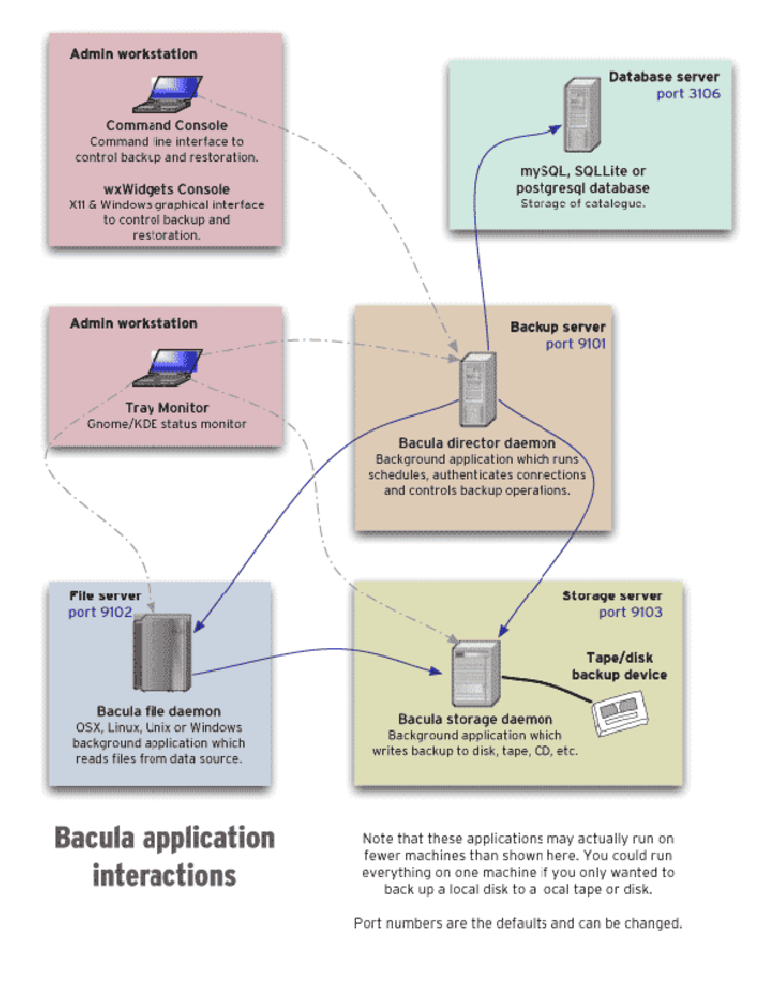
\includegraphics{./bacula-applications.eps} 
(remerciements \`a Aristedes Maniatis pour ce sch\'ema et le suivant) 

\begin{itemize}
\item 
   \label{DirDef}
   Le service {\bf Bacula Director
\label{a1}
} est le programme qui supervise toutes  les op\'erations de sauvegarde,
restauration, v\'erification et archivage.  L'administrateur syst\`eme utilise
le Bacula Director pour planifier les  sauvegardes et restaurer les fichiers.
Pour plus de d\'etails, consultez la section concernant la conception du Daemon Director 
dans la documentation pour d\'eveloppeurs. Le Director est ex\'ecut\'e en tant que {\it daemon} 
ou service (c'est \`a dire en t�che de fond).
\item 
   \label{UADef}
   Le service {\bf Bacula Console} est le programme qui permet \`a 
l'administrateur ou \`a l'utilisateur de communiquer avec le {\bf Bacula 
Director} (voir ci-dessus). Actuellement, le service Bacula Console  est
disponible en trois versions. La premi\`ere et la plus simple est 
d'ex\'ecuter le programme Console dans une fen\^etre shell (i.e. interface
TTY).  La plupart des administrateurs syst\`eme trouveront cette m\'ethode
parfaitement  ad\'equate. La seconde version est une interface graphique GNOME
qui est loin d'\^etre compl\`ete, mais est
tout \`a fait  fonctionnelle puisqu'elle poss\`ede la plupart des
possibilit\'es de la Console  shell. La troisi\`eme version est une interface
graphique wxWidgets qui permet de s\'electionner  interactivement les fichiers
\`a restaurer. Elle int\`egre la plupart des fonctionnalit\'es  de la console
shell, permet la compl\'etion automatique avec la touche tabulation, et 
fournit une aide instantan\'ee relative \`a la commande que vous \^etes en
train de taper.  Pour plus de d\'etails, consultez la section 
\ilink{Conception de la Console Bacula}{_ConsoleChapter} dans la documentation 
pour d\'eveloppeurs. 
\item 
   \label{FDDef}
   Le service {\bf Bacula File} (ou programme client) est le programme install\'e
sur la machine \`a sauvegarder. Il est sp\'ecifique au syst\`eme sur lequel
il est  ex\'ecut\'e et a la charge de fournir les attributs des fichiers et
les donn\'ees  requis par le Director. Les Services File sont aussi charg\'es
de la partie  d\'ependant du syst\`eme de fichiers lors de la restauration des
attributs de  fichiers et des donn\'ees. Pour plus de d\'etails, consultez le
document  sur la conception du File Daemon dans le Guide pour Developpeurs. Ce
programme est ex\'ecut\'e en  tant que service sur la machine \`a sauvegarder,
et la documentation s'y r\'ef\`ere  parfois en tant que Client (par exemple
dans les fichiers de configuration de  Bacula). En plus du File Daemon pour
Unix/Linux, il existe un File Daemon pour  Windows (usuellement distribu\'e au
format binaire). Le File Daemon Windows  fonctionne sur toutes les versions
actuelles de Windows (NT,  2000, XP, 2003 et peut-\^etre aussi 98 et Me). 
\item 
   \label{SDDef}
   Le service {\bf Bacula Storage} est le programme qui transf\`ere les donn\'ees
et  les attributs de fichiers aux m\'edia physiques ou aux volumes et les
restitue  lors de restaurations. En d'autres termes, Le storage Daemon est
responsable  des op\'erations de lecture et d'\'ecriture sur vos cartouches (ou
autres m\'edia  de stockage, comme par exemple des fichiers). Pour plus de 
d\'etails consultez la  Documentation Pour D\'eveloppeurs sur la conception du 
Storage Daemon. 
\item 
   \label{DBDefinition}
   Les services {\bf Catalogue} ont pour t\^ache de maintenir \`a jour la base de
donn\'ees des index de fichiers et volumes pour tous les fichiers
sauvegard\'es.  Les services {\bf Catalogue} permettent \`a l'administrateur
syst\`eme ou \`a  l'utilisateur de localiser rapidement et restaurer n'importe
quel fichier.  Les services Catalogue de Bacula le placent dans une
cat\'egorie diff\'erente  de programmes tels que tar et bru, puisque le
catalogue Bacula maintient  un enregistrement de chaque  volume utilis\'e,
chaque job ex\'ecut\'e et chaque fichier sauvegard\'e  ce qui permet des
restaurations et une gestion de volumes efficaces. Bacula  supporte
actuellement trois bases de donn\'ees diff\'erentes, MySQL, PostgreSQL,  et
SQLite. L'une des trois doit \^etre choisie \`a la compilation de {\bf
Bacula}.  

Les trois bases de donn\'ees actuellement support\'ees (MySQL, PostgreSQL, ou
SQLite)  fournissent de nombreuses fonctions telles l'indexation rapide,
requ\^etes  arbitraires, et s\'ecurit\'e. Bien que nous pr\'evoyions de
supporter d'autres  bases de donn\'ees SQL majeures, l'impl\'ementation
actuelle s'interface seulement  avec MySQL, PostgreSQL, et SQLite. Pour plus
de d\'etails consultez le  
\ilink{document sur la conception des Services Catalogue
}{_ChapterStart30}.  

Les RPMs pour MySQL et PostgreSQL font partie de la distribution Red Hat. 
Sinon, il est tout \`a fait ais\'e de les construire \`a partir des sources. 
Consultez le chapitre 
\ilink{ Installer et configurer MySQL}{_ChapterStart}  ou 
\ilink{ Installer et configurer PostgreSQL}{_ChapterStart10} de
ce  document pour plus de d\'etails. Pour plus d'informations sur MySQL et
PostgreSQL,  consultez 
\elink{www.mysql.com}{http://www.mysql.com} ou 
\elink{www.postgresql.org}{http://www.postgresql.org}.  

Configurer et construire SQLite est encore plus facile. Pour les d\'etails  de
configuration de SQLite, consultez le chapitre 
\ilink{Installer et Configurer SQLite}{_ChapterStart33} de ce
document. 
\item 
   \label{MonDef}
   Le service {\bf Bacula Monitor} est le programme qui permet \`a
l'administrateur  ou \`a l'utilisateur de contr\^oler le statut des {\it
daemons} Bacula ({\bf Bacula Directors},  {\bf Bacula File Daemons} et {\bf
Bacula Storage Daemons}) (voir ci-dessus). Actuellement,  la seule version
disponible est une version GTK+, qui fonctionne avec Gnome et KDE (ainsi  que
tout gestionnaire de fen\^etre qui respecte le standard system tray
FreeDesktop.org). 
\end{itemize}

Pour r\'ealiser avec succ\`es les op\'erations de sauvegarde et restauration,
les quatre services suivants doivent \^etre configur\'es et lanc\'es : le
Director Daemon, le File Daemon, le Storage Daemon et MySQL, PostgreSQL ou
SQLite. 

\section{Configuration de Bacula}
\index[general]{Configuration de Bacula }
\index[general]{Bacula!Configuration de }
\addcontentsline{toc}{section}{Configuration de Bacula}

Pour que Bacula comprenne votre syst\`eme, quels clients vous voulez
sauvegarder et comment, vous devez cr\'eer un certain nombre de fichiers de
configuration. La suite brosse un tableau de ces op\'erations. 

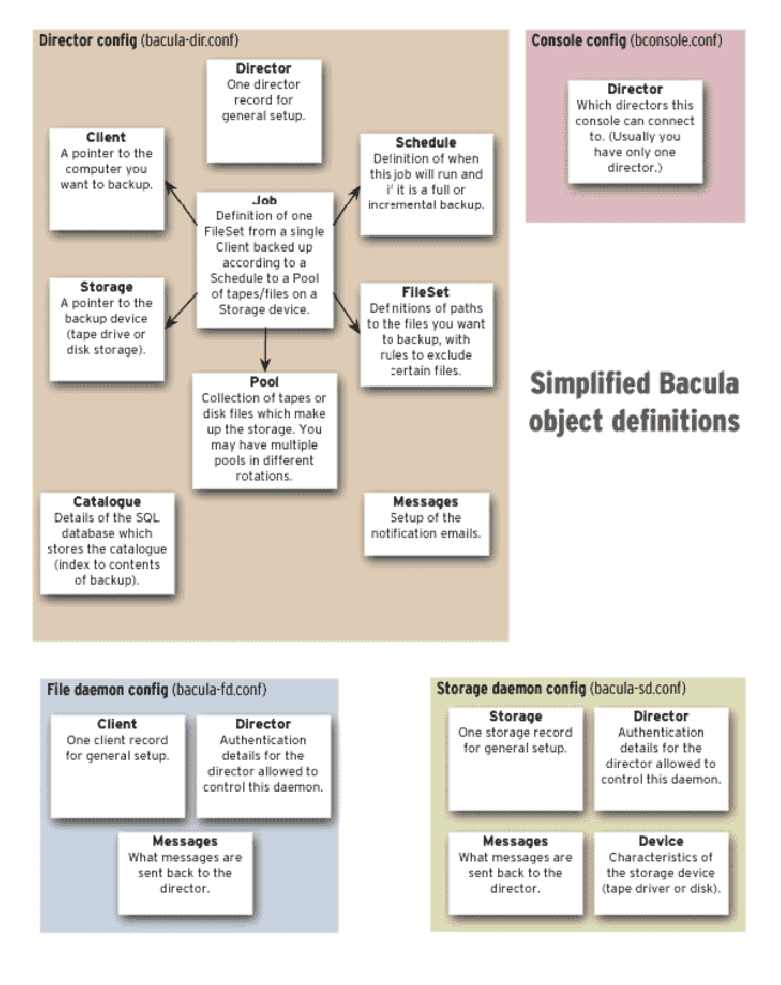
\includegraphics{./bacula-objects.eps} 

\section{Conventions utilis\'ees dans ce document}
\index[general]{Conventions utilis\'ees dans ce document }
\index[general]{Document!Conventions utilis\'ees dans ce }
\addcontentsline{toc}{section}{Conventions utilis\'ees dans ce document}

{\bf Bacula} est en constante \'evolution, par cons\'equent, ce manuel ne sera
pas toujours en accord avec le code. Si un objet de ce manuel est
pr\'ec\'ed\'e d'un ast\'erisque (*), cela signifie que cette fonctionnalit\'e
particuli\`ere n'est pas impl\'ement\'ee. S'il est pr\'ec\'ed\'e d'un signe
plus (+), cela indique que la fonction est peut-\^etre partiellement
impl\'ement\'ee. 

Si vous lisez la version de ce manuel fournie avec les sources de Bacula, le
paragraphe ci-dessus reste vrai. En revanche, si vous lisez la version en
ligne : 
\elink{www.bacula.org/manual}{http://www.bacula.org/manual}, veuillez garder
\`a l'esprit que cette version d\'ecrit la version courante de d\'eveloppement
de Bacula (celle du CVS) qui peut contenir des fonctionnalit\'es qui
n'existent pas dans la version "officielle". De m\^eme, il est
g\'en\'eralement un peu \`a la tra{\^\i}ne derri\`ere le code. 

\section{D\'emarrage rapide}
\index[general]{D\'emarrage rapide }
\index[general]{Rapide!D\'emarrage }
\addcontentsline{toc}{section}{D\'emarrage rapide}

Pour faire fonctionner Bacula rapidement, nous vous recommandons de commencer
par parcourir la section Terminologie ci-dessous, de passer rapidement en
revue le chapitre suivant intitul\'e 
\ilink{L'\'etat actuel de Bacula}{_ChapterStart2}, puis le 
\ilink{Guide de d\'emarrage rapide de Bacula}{_ChapterStart37},
qui vous donnera une vue d'ensemble de la mise en oeuvre de Bacula . Apr\`es
quoi vous devriez poursuivre avec le chapitre sur 
\ilink{ L'installation de Bacula}{_ChapterStart17}, puis le chapitre
\ilink{Comment configurer Bacula}{_ChapterStart16}, et finalement,
le chapitre  \ilink{Ex\'ecuter Bacula}{_ChapterStart1}. 

\section{Terminologie}
\index[general]{Terminologie }
\addcontentsline{toc}{section}{Terminologie}

Pour faciliter la communication autour de ce projet, nous fournissons ici les
d\'efinitions de la terminologie que nous utilisons. 

\begin{description}

\item [Administrateur]
   \index[sd]{Administrateur }
   La ou les personne(s) responsable(s) de l'administration  du syst\`eme Bacula.


\item [Sauvegarde]
   \index[sd]{Sauvegarde }
   Nous utilisons ce terme pour un job Bacula qui sauvegarde des  fichiers. 

\item [Fichier Bootstrap (Bootstrap File)]
   \index[sd]{Fichier Bootstrap (Bootstrap File) }
   Le bootstrap est un fichier ASCII qui  contient, sous une forme compacte, les
commandes qui permettent \`a Bacula ou \`a  l'utilitaire autonome {\bf
bextract} de restaurer les contenus d'un ou plusieurs  volumes, par exemple,
l'\'etat courant d'un syst\`eme qui vient d'\^etre sauvegard\'e.  Avec un
fichier bootstrap, Bacula peut restaurer votre syst\`eme sans catalogue.  Vous
pouvez cr\'eer un fichier bootstrap depuis un catalogue pour extraire le
fichier  que vous voulez. 

\item [Catalogue]
   \index[sd]{Catalogue }
   Le catalogue est utilis\'e pour stocker des informations sommaires  concernant
les Jobs et Clients, les fichiers qui ont \'et\'e sauvegard\'es ainsi que le 
ou les volume(s) o\`u ils ont \'et\'e sauvegard\'es. L'information stock\'ee
dans le  catalogue permet \`a l'administrateur ou aux utilisateurs de
d\'eterminer quels jobs  ont \'et\'e ex\'ecut\'es, leur statut, ainsi que
d'importantes caract\'eristiques de chaque  fichier sauvegard\'e. Le catalogue
est une ressource en ligne, mais ne contient pas  les donn\'ees pour les
fichiers sauvegard\'es. La plupart des informations stock\'ees  dans le
catalogue le sont aussi sur les volumes de sauvegarde (i.e. cartouches).  Bien
sur, les cartouches auront aussi une copie du fichier en plus de ses attributs
 (voir ci-dessus).  

La fonction Catalogue est de celles qui distinguent Bacula de simples
programmes  de sauvegarde et archivage tels que {\bf dump} et {\bf tar}. 

\item [Client]
   \index[sd]{Client }
   Dans la terminologie de Bacula, le mot Client d\'esigne une machine 
sauvegard\'ee, et est synonyme de File service ou File Daemon. Nous nous y
r\'ef\'erons  assez souvent par "le FD". Un client est d\'efini dans une
ressource de fichier de  configuration. 

\item [Console]
   \index[sd]{Console }
   Le programme qui interface le Director, permettant \`a  l'administrateur de
contr\^oler Bacula. 

\item [Daemon]
   \index[sd]{Daemon }
   Terminologie Unix pour un programme toujours pr\'esent en arri\`ere plan  pour
prendre en charge une t\^ache donn\'ee. Sur les syst\`emes Windows, ainsi que
certains  Linux, les {\it daemons} sont appel\'es {\bf Services}. 

\item [Directive]
   \index[sd]{Directive }
   Le terme directive est utilis\'e pour d\'esigner une entr\'ee ou
enregistrement \`a l'int\'erieur d'une ressource dans un fichier de 
configuration qui d\'efinit un \'el\'ement sp\'ecifique. Par exemple, la
directive  {\bf Name} d\'efinit le nom de la ressource. 

\item [Director]
   \index[sd]{Director }
   Le principal {\it daemon} serveur de Bacula qui planifie et dirige  toutes
les op\'erations de Bacula. Occasionnellement, nous le d\'esignons par "le
DIR". 

\item [Differentielle (Differential)]
   \index[sd]{Differentielle (Differential) }
   Une sauvegarde qui inclut tous les fichiers  modifi\'es depuis le lancement de
la derni\`ere sauvegarde compl\`ete (Full).  Notez que d'autres logiciels de
sauvegarde peuvent d\'efinir ceci diff\'eremment.  

\item [Attributs de fichiers]
   \index[sd]{Attributs de fichiers }
   Les Attributs de fichiers sont toutes les  informations n\'ecessaires au sujet
d'un fichier pour l'identifier, et toutes ses  propri\'et\'es telles taille,
date de cr\'eation, date de modification, permission, etc.  En principe, les
attributs sont int\'egralement manipul\'es par Bacula de sorte que 
l'utilisateur n'a jamais \`a s'en pr\'eoccuper. Les attributs n'incluent pas
les donn\'ees  du fichier. 

\item [File Daemon]
   \index[sd]{File Daemon }
   Le {\it daemon} ex\'ecut\'e sur l'ordinateur client \`a sauvegarder. Il est 
aussi d\'esign\'e par Service Fichier (File Service) et parfois Service Client
ou FD. 

\item [
   \label{FileSetDef}
   FileSet]
\index[sd]{a name }
Un FileSet est une ressource d'un fichier de configuration qui  d\'efinit les
fichiers \`a sauvegarder. Il consiste en une liste de fichiers ou 
r\'epertoires inclus, une liste de fichiers ou r\'epertoires exclus et la
fa\c{c}on dont les  fichiers seront stock\'es (compression, chiffrement,
signatures). Pour plus de d\'etails  consultez le paragraphe 
\ilink{D\'efinition de la Ressource FileSet}{FileSetResource}
dans le chapitre Director de ce document. 

\item [Incrementale]
   \index[sd]{Incrementale }
   Une sauvegarde qui inclut tous les fichiers modifi\'es depuis  le lancement de
la derni\`ere sauvegarde compl\`ete (Full), diff\'erentielle, ou 
incr\'ementale. Normalement sp\'ecifi\'e dans la directive {\bf Level}
(niveau) dans la  d\'efinition de la ressource Job, ou dans une ressource
Schedule. 

\item [
   \label{JobDef}
   Job]
\index[sd]{a name }
Un Job Bacula est une ressource de configuration qui d\'efinit le  travail que
Bacula doit effectuer pour sauvegarder ou restaurer un client  particulier. Un
Job consiste en un {\bf Type}, (Type : backup, restore, verify, etc.),  un
{\bf Niveau} (Level : full, incremental, ...), un {\bf FileSet}, et un lieu de
{\bf Stockage} o\`u \'ecrire les fichiers (Storage device, Media Pool). Pour
plus de  d\'etails consultez le chapitre 
\ilink{D\'efinition des Ressources Job}{JobResource} de ce
document. 

\item [Monitor]
   \index[sd]{Monitor }
   Le programme qui s'interface avec chacun des {\it daemons} pour permettre \`a 
l'utilisateur ou \`a l'administrateur de surveiller le statut de Bacula.  

\item [Resource]
   \index[sd]{Resource }
   Une ressource est une partie d'un fichier de configuration qui  d\'efinit une
unit\'e sp\'ecifique d'information disponible pour Bacula. Par exemple,  la
ressource {\bf Job} d\'efinit toutes les propri\'et\'es d'un Job sp\'ecifique
:  nom, schedule (planification), volume pool, type de sauvegarde, niveau de 
sauvegarde, etc. 

\item [Restore]
   \index[sd]{Restore }
   Une Restore est une ressource de configuration qui d\'ecrit  l'op\'eration de
restauration d'un fichier (perdu ou endommag\'e) depuis un  medium de
sauvegarde. C'est l'op\'eration r\'eciproque d'une sauvegarde,  sauf que, dans
la plupart des cas, une restauration concernera un petit  ensemble de fichiers
tandis qu'une sauvegarde concerne le plus souvent  l'ensemble des fichiers
d'un syst\`eme. Bien sur, apr\`es une d\'efaillance  de disque(s), Bacula peut
\^etre appel\'e \`a effectuer une restauration compl\`ete  de tous les
fichiers qui \'etaient sur le syst\`eme. 

\item [Schedule]
   \index[sd]{Schedule }
   Un Schedule est une ressource de configuration qui d\'efinit  le moment de
l'ex\'ecution du Job Bacula. Pour utiliser un schedule, la ressource  Job se
r\'ef\`ere au nom du Schedule. Pour plus de d\'etails, consultez la  
\ilink{D\'efinition de la ressource Schedule}{ScheduleResource} 
dans le chapitre Director de ce document. 

\item [Service]
   \index[sd]{Service }
   Terminologie Windows pour d\'esigner un {\it daemon} -- Voir  plus haut. Elle
est maintenant fr\'equemment utilis\'ee dans les environnements  Unix aussi. 

\item [Adresses de stockage]
   \index[sd]{Adresses de stockage }
   Les informations retourn\'ees par les Storage  services qui localisent de
fa\c{c}on unique les fichiers sur un medium de  sauvegarde. Elles consistent
en deux parties : l'une appartient \`a chaque  fichier sauvegard\'e, l'autre
\`a l'ensemble du Job. Normalement, cette information  est sauvegard\'ee dans
le catalogue de sorte que l'utilisateur n'a pas besoin  de connaissances
particuli\`eres des adresses de stockage. L'adresse de stockage  inclut les
attributs de fichiers (voir plus haut) ainsi que la localisation  unique de
l'information sur le volume de sauvegarde. 

\item [Storage Daemon]
   \index[sd]{Storage Daemon }
   Le Storage Daemon, parfois d\'esign\'e par "SD" est le  programme qui
\'ecrit les attributs et les donn\'ees sur un Volume de Stockage  (Storage
Volume) (Usuellement une cartouche ou un disque). 

\item [Session]
   \index[sd]{Session }
   D\'esigne en principe le dialogue interne entre le File Daemon  et le Storage
Daemon. Le File Daemon ouvre une {\bf session} avec le  Storage Daemon pour
sauvegarder un Fileset, ou pour le restaurer. Une session  est associ\'ee \`a
un et un seul Job Bacula (voir plus haut). 

\item [Verify]
   \index[sd]{Verify }
   Il s'agit d'un job qui compare les attributs du fichier actuel  aux attributs
qui ont \'et\'e pr\'ealablement stock\'es dans le catalogue Bacula.  Cette
fonction peut \^etre utilis\'ee pour d\'etecter les modifications de
syst\`emes  de fichiers critiques, \`a la fa\c{c}on de {\bf Tripwire}. L'un
des avantages  majeurs de l'utilisation de Bacula pour cette t\^ache est que
sur la machine  que vous voulez prot\'eger, vous pouvez n'ex\'ecuter que le
File Daemon. Le  Director, le Storage Daemon et le catalogue peuvent r\'esider
sur une autre  machine. Par cons\'equent si votre serveur est un jour
compromis, il est peu  probable que la base de donn\'ees de v\'erification ait
\'et\'e trifouill\'ee.  

Verify peut aussi \^etre utilis\'e pour s'assurer que les donn\'ees les plus 
r\'ecemment \'ecrites sur un volume sont coh\'erentes avec ce qui figure dans
le  catalogue (c-\`a-d il compare les attributs de fichiers), ou encore,
confronter le contenu du volume aux fichiers originaux sur le disque. 

\item [*Archive]
   \index[sd]{*Archive }
   Une op\'eration d'archivage est effectu\'ee apr\`es une sauvegarde,  et
consiste en l'exclusion des volumes sur lesquels les donn\'ees sont
sauvegard\'ees  de l'utilisation courante. Ces volumes sont marqu\'es
"Archived", et ne sont plus  utilis\'es pour sauvegarder des fichiers. Tous
les fichiers contenus sur un Volume  Archive sont supprim\'es du catalogue.
PAS ENCORE IMPLEMENTE. 

\item [*Update]
   \index[sd]{*Update }
   Une op\'eration Update synchronise les fichiers du syst\`eme distant  sur ceux
du local. Ceci est l'\'equivalent d'une fonctionnalit\'e {\bf rdist}. PAS 
ENCORE IMPLEMENTE. 

\item [P\'eriode de r\'etention]
   \index[sd]{P\'eriode de r\'etention }
   Bacula reconnait plusieurs sortes de p\'eriodes de r\'etention.  Les plus
importantes sont la p\'eriode de r\'etention des fichiers, la p\'eriode de 
r\'etention des jobs et la p\'eriode de r\'etention des volumes. Chacune de
ces p\'eriodes  de r\'etention d\'esigne la dur\'ee pendant laquelle
l'enregistrement sp\'ecifique sera  conserv\'e dans le catalogue. Ceci ne doit
pas \^etre confondu avec le temps pendant  lequel les donn\'ees sauvegard\'ees
sur un volume sont valides. 

La p\'eriode de  r\'etention des fichiers d\'etermine la dur\'ee pendant
laquelle les enregistrements  concernant les fichiers seront gard\'es dans le
catalogue. Cette p\'eriode est importante  car le volume des enregistrements
relatifs aux fichiers occupe, de loin, le plus  d'espace dans la base de
donn\'ees. Par cons\'equent, vous devez vous assurer qu'un  "\'elagage"
(NDT : pruning) r\'egulier de ces enregistrements est  effectu\'e. (Voir la
commande {\bf retention} de la Console pour plus de d\'etails  sur ce sujet). 

La p\'eriode de r\'etention des jobs est la dur\'ee pendant laquelle  les
enregistrements relatifs aux jobs seront conserv\'es dans le catalogue. Notez 
que tous les enregistrements relatifs aux fichiers sont attach\'es aux jobs
qui ont  sauvegard\'e ces fichiers. Les enregistrements relatifs aux fichiers
peuvent \^etre  purg\'es tout en conservant ceux relatifs aux jobs. Dans ce
cas, l'information  concernant les jobs ex\'ecut\'es restera disponible, mais
pas les d\'etails des fichiers  sauvegard\'es. Normalement, lorsqu'un job est
purg\'e, tous les enregistrements  concernant les fichiers qu'il a
sauvegard\'e le sont aussi. 

La p\'eriode de r\'etention  des volumes est la
dur\'ee minimale de conservation d'un volume avant qu'il ne soit 
r\'eutilis\'e. Bacula n'effacera, en principe, jamais un volume qui contient
la seule  copie de sauvegarde d'un fichier. Dans les conditions id\'eales, le
catalogue  maintiendrait les entr\'ees pour tous les fichiers sauvegard\'es
pour tous les  volumes courants. Une fois qu'un volume est \'ecras\'e, les
fichiers qui \'etaient  sauvegard\'es dessus sont automatiquement effac\'es du
catalogue. Cependant, s'il y a  un tr\`es gros pool de volumes ou si un volume
n'est jamais \'ecras\'e, le catalogue  pourrait devenir \'enorme. Pour
maintenir le catalogue dans des proportions g\'erables,  les informations de
sauvegarde devraient \^etre supprim\'ees apr\`es une p\'eriode de  r\'etention
des fichiers d\'efinie. 

\item [Scan]
   \index[sd]{Scan }
   Une op\'eration de scan consiste en un balayage du contenu d'un  volume ou
d'une s\'erie de volumes. Ces volumes et les informations concernant les 
fichiers qu'ils contiennent sont restaur\'es vers le catalogue Bacula. Une
fois ces  informations restaur\'ees, les fichiers sauvegard\'es sur ces
volumes pourront \^etre  ais\'ement restaur\'es. Cette fonction est
particuli\`erement utile si certains volumes  ou jobs ont d\'epass\'e leur
p\'eriode de r\'etention et ont \'et\'e \'elagu\'es ou  purg\'es du
catalogue. Le balayage des donn\'ees des volumes est effectu\'e en utilisant 
le programme {\bf bscan}. Consultez la 
\ilink{section bscan }{bscan}  du chapitre sur les utilitaires
Bacula de ce manuel pour plus de d\'etails. 

\item [Volume]
   \index[sd]{Volume }
   Un volume est une unit\'e d'archivage, usuellement une cartouche ou  un
fichier nomm\'e sur disque o\`u Bacula stocke les donn\'ees pour un ou
plusieurs jobs  de sauvegarde. Tous les volumes Bacula ont un label unique
(logiciel) \'ecrit sur le  volume par Bacula afin qu'il puisse \^etre assur\'e de 
lire le bon volume.  (En principe, il ne devrait pas y avoir de
confusion avec des fichiers disques, mais  avec des cartouches, il est facile
de monter la mauvaise). 
\end{description}

\section{Ce que Bacula n'est pas}
\index[general]{Ce que Bacula n'est pas }
\index[general]{Pas!Ce que Bacula n'est }
\addcontentsline{toc}{section}{Ce que Bacula n'est pas}

{\bf Bacula} est un programme de sauvegarde, restauration et v\'erification,
ce n'est pas un syst\`eme complet de disaster recovery
\label{c}
\`a lui seul, mais il peut en \^etre une partie clef si vous planifiez
soigneusement et suivez les instructions incluses dans le chapitre 
\ilink{ Plan de reprise d'activit\'e avec Bacula}{_ChapterStart38} de
ce manuel. 

Avec la planification appropri\'ee, telle que d\'ecrite dans le chapitre sur le
plan de reprise d'activit\'e, {\bf Bacula} peut devenir la pi\`ece centrale de
votre plan de reprise d'activit\'e. Par exemple, si vous avez cr\'e\'e un(e)
disque(tte) boot d'urgence et un(e) disque(tte) de secours Bacula pour
sauvegarder les informations de partitionnement courantes de votre disque dur,
et maintenu un jeu de sauvegardes complet de votre syst\`eme, il est possible
de reconstruire compl\`etement votre syst\`eme "depuis le m\'etal brut" 
(NDT : From bare metal)
\label{d1}
. 

Si vous avez utilis\'e la directive {\bf WriteBootstrap} dans votre job ou
quelque autre moyen pour sauvegarder un fichier bootstrap valide, vous pourrez
l'utiliser pour extraire les fichiers n\'ecessaires (sans utiliser le
catalogue et sans chercher manuellement les fichiers \`a restaurer). 

\section{Interactions entre les services Bacula}
\index[general]{Bacula!Interactions entre les services }
\index[general]{Interactions entre les services Bacula }
\addcontentsline{toc}{section}{Interactions entre les services Bacula}

Le diagramme fonctionnel suivant montre les interactions typiques entre les
services Bacula pour un job de type sauvegarde. Chaque bloc repr\'esente en
g\'en\'eral un processus s\'epar\'e (normalement un {\it daemon}). En
g\'en\'eral, le director surveille le flux d'informations. Il maintient aussi
le catalogue. 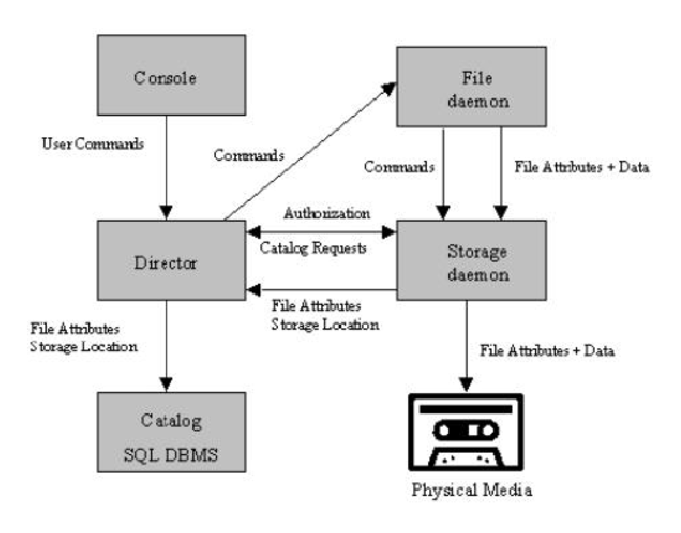
\includegraphics{./flow.eps} 

  %%
%%

\chapter{The Current State of Bacula}
\label{StateChapter}
\index[general]{Current State of Bacula }

In other words, what is and what is not currently implemented and functional. 

\section{What is Implemented}
\index[general]{Implemented!What}
\index[general]{What is Implemented}

\begin{itemize}
\item Job Control
   \begin{itemize}
   \item Network backup/restore with centralized Director.  
   \item Internal scheduler for automatic 
      \ilink{Job}{JobDef} execution.  
   \item Scheduling of multiple Jobs at the same time.  
   \item You may run one Job at a time or multiple simultaneous Jobs
         (sometimes called multiplexing).
   \item Job sequencing using priorities.  
   \item \ilink{Console}{UADef} interface to the Director allowing complete
      control.  A shell, Qt4 GUI, wxWidgets GUI and Web versions of
      the Console program are available.  Note, the Qt4 GUI program called
      the Bacula Administration tool or bat, offers many additional
      features over the shell program.
   \end{itemize}

\item Security
   \begin{itemize}
   \item Verification of files previously cataloged, permitting a Tripwire like 
      capability (system break-in detection).  
   \item CRAM-MD5 password authentication between each component (daemon).
   \item Configurable 
      \ilink{TLS (SSL) communications encryption}{CommEncryption} between each 
            component.
   \item Configurable
   \ilink{Data (on Volume) encryption}{DataEncryption}
      on a Client by Client basis.
   \item Computation of MD5 or SHA1 signatures of the file data if requested.  
   \end{itemize}


\item Restore Features
   \begin{itemize}
   \item Restore of one or more files selected interactively either for the
      current backup or a backup prior to a specified time and date.  
   \item Restore of a complete system starting from bare  metal. This is mostly
      automated for Linux systems and  partially automated for Solaris. See 
      \ilink{Disaster Recovery Using Bacula}{RescueChapter}. This is also
      reported to work on Win2K/XP systems.  
   \item Listing and Restoration of files using stand-alone {\bf bls} and {\bf
        bextract} tool programs. Among other things, this permits extraction of
      files when Bacula and/or the catalog are not available. Note, the
      recommended way to restore files is using the restore command in the
      Console. These programs are designed for use as a last resort.
   \item Ability to restore the catalog database rapidly by using bootstrap
      files (previously saved).
   \item Ability to recreate the catalog database by scanning backup Volumes 
      using the {\bf bscan} program.  
   \end{itemize}

\item SQL Catalog
   \begin{itemize}
   \item Catalog database facility for remembering Volumes, Pools, Jobs,  and
      Files backed up.  
   \item Support for MySQL, PostgreSQL, and SQLite Catalog databases.  
   \item User extensible queries to the MySQL, PostgreSQL and SQLite databases.  
   \end{itemize}

\item Advanced Volume and Pool Management
   \begin{itemize}
   \item Labeled Volumes, preventing accidental overwriting  (at least by
      Bacula).  
   \item Any number of Jobs and Clients can be backed up to a single  Volume.
      That is, you can backup and restore Linux, Unix, Sun, and  Windows machines to
      the same Volume.  
   \item Multi-volume saves. When a Volume is full, {\bf Bacula}  automatically
      requests the next Volume and continues the backup.  
   \item 
      \ilink{Pool and Volume}{PoolResource} library management 
      providing Volume flexibility (e.g. monthly, weekly, daily Volume sets,  Volume
      sets segregated by Client, ...). 
   \item Machine independent Volume data format. Linux, Solaris, and Windows 
      clients can all be backed up to the same Volume if desired. 
   \item The Volume data format is upwards compatible so that old Volumes
      can always be read.
   \item A flexible 
      \ilink{message}{MessagesChapter}  handler including routing
      of messages from any daemon back to the  Director and automatic email
      reporting.  
   \item Data spooling to disk during backup with subsequent write to tape from
      the spooled disk files. This prevents tape "shoe shine"  during
      Incremental/Differential backups.  
   \end{itemize}

\item Advanced Support for most Storage Devices
    \begin{itemize}
   \item Autochanger support using a simple shell interface that can interface 
      to virtually any autoloader program. A script for {\bf mtx} is  provided.  
   \item Support for autochanger barcodes -- automatic tape labeling from 
      barcodes.  
   \item Automatic support for multiple autochanger magazines either using
      barcodes or by reading the tapes.  
   \item Support for multiple drive autochangers.
   \item Raw device backup/restore. Restore must be to the same device. 
   \item All Volume blocks (approximately 64K bytes) contain a data checksum.  
   \item Migration support -- move data from one Pool to another or
         one Volume to another.
   \item Supports writing to DVD.
   \end{itemize}

\item Multi-Operating System Support
   \begin{itemize} 
   \item Programmed to handle arbitrarily long filenames and messages.  
   \item GZIP compression on a file by file basis done by the Client program  if
      requested before network transit.  
    \item Saves and restores POSIX ACLs and Extended Attributes on most OSes if
      enabled.
   \item Access control lists for Consoles that permit restricting user access
      to only their data.  
   \item Support for save/restore of files larger than 2GB.  
   \item Support for 64 bit machines, e.g. amd64, Sparc.
   \item Support ANSI and IBM tape labels.
   \item Support for Unicode filenames (e.g. Chinese) on Win32 machines
   \item Consistent backup of open files on Win32 systems (WinXP, Win2003, 
         and Vista)
         but not Win2000, using Volume Shadow Copy (VSS).
   \item Support for path/filename lengths of up to 64K on Win32 machines
         (unlimited on Unix/Linux machines).
   \end{itemize}

\item Miscellaneous
   \begin{itemize}
   \item Multi-threaded implementation.  
   \item A comprehensive and extensible 
      \ilink{configuration file}{DirectorChapter} for each daemon.  
   \end{itemize}
\end{itemize}

\section{Advantages Over Other Backup Programs}
\index[general]{Advantages of Bacula Over Other Backup Programs }
\index[general]{Programs!Advantages of Bacula Over Other Backup }

\begin{itemize}
\item Since there is a client for each machine, you can backup
   and restore clients of any type ensuring that all attributes
   of files are properly saved and restored.
\item It is also possible to backup clients without any client
   software by using NFS or Samba.  However, if possible, we
   recommend running a Client File daemon on each machine to be
   backed up.
\item Bacula handles multi-volume backups.  
\item A full comprehensive SQL standard database of all files backed up.  This
   permits online viewing of files saved on any particular  Volume.  
\item Automatic pruning of the database (removal of old records) thus 
   simplifying database administration.  
\item Any SQL database engine can be used making Bacula very flexible.  
      Drivers currently exist for MySQL, PostgreSQL, and SQLite.
\item The modular but integrated design makes Bacula very scalable.  
\item Since Bacula uses client file servers, any database or
   other application can be properly shutdown by Bacula using the
   native tools of the system, backed up, then restarted (all
   within a Bacula Job).
\item Bacula has a built-in Job scheduler.  
\item The Volume format is documented and there are simple C programs to 
   read/write it.  
\item Bacula uses well defined (IANA registered) TCP/IP ports -- no rpcs,  no
   shared memory.  
\item Bacula installation and configuration is relatively simple compared  to
   other comparable products.  
\item According to one user Bacula is as fast as the big major commercial 
   applications.  
\item According to another user Bacula is four times as fast as another
   commercial application, probably because that application  stores its catalog
   information in a large number of individual  files rather than an SQL database
   as Bacula does.  
\item Aside from several GUI administrative interfaces, Bacula has a
   comprehensive shell administrative interface, which allows the
   administrator to use tools such as ssh to administrate any part of
   Bacula from anywhere (even from home).
\item Bacula has a Rescue CD for Linux systems with the following features:  
   \begin{itemize}
   \item You build it on your own system from scratch with one simple  command:
      make -- well, then make burn. 
   \item It uses your kernel  
   \item It captures your current disk parameters and builds scripts that  allow
      you to automatically repartition a disk and format it to  put it back to what
      you had before. 
   \item It has a script that will restart your networking (with the right  IP
      address)  
   \item It has a script to automatically mount your hard disks.  
   \item It has a full Bacula FD statically linked  
   \item You can easily add additional data/programs, ... to the disk.  
   \end{itemize}

\end{itemize}

\section{Current Implementation Restrictions}
\index[general]{Current Implementation Restrictions }
\index[general]{Restrictions!Current Implementation }

\begin{itemize}
\item It is very unusual to attempt to restore two Jobs
   that ran simultaneously in a single restore, but if
   you do, please be aware that unless you had
   data spooling turned on and the spool file held the full
   contents of both Jobs during the backup, the restore will not
   work correctly. In other terms, Bacula cannot restore
   two jobs in the same restore if the Jobs' data blocks were
   intermixed on the backup medium. The problem is resolved by
   simply doing two restores, one for each Job. 
\item Bacula can generally restore any backup made from one client
   to any other client. However, if the architecture is significantly
   different (i.e. 32 bit architecture to 64 bit or Win32 to Unix),
   some restrictions may apply (e.g. Solaris door files do not exist
   on other Unix/Linux machines; there are reports that Zlib compression
   written with 64 bit machines does not always read correctly on a 32 bit
   machine).
\end{itemize}

\section{Design Limitations or Restrictions}
\index[general]{Restrictions!Design Limitations or }
\index[general]{Design Limitations or Restrictions }

\begin{itemize}
\item Names (resource names, Volume names, and such) defined in Bacula 
   configuration files are limited to a fixed number of
   characters.  Currently the limit is defined as 127 characters.  Note,
   this does not apply to filenames, which may be arbitrarily long.
\item Command line input to some of the stand alone tools -- e.g. btape,
   bconsole is restricted to several hundred characters maximum.
\end{itemize}

\section{Items to Note}
\index[general]{Items to Note}
\begin{itemize}
\item Bacula's Differential and Incremental \textsl{normal} backups are based
  on time stamps.  Consequently, if you move files into an existing directory
  or move a whole directory into the backup fileset after a Full backup, those
  files will probably not be backed up by an Incremental save because they will
  have old dates.  This problem is corrected by using Accurate mode backups
  or by explicitly updating the date/time stamp on all moved files.
\item In older versions of Bacula ($<=$ 3.0.x), if you have over 4 billion file
  entries stored in your database, the database FileId is likely to overflow.
\item In non \textsl{Accurate} mode, files deleted after a Full save will be
  included in a restoration. This is typical for most similar backup programs.
\end{itemize}


If you are like me, you want to get Bareos running immediately to get a feel
for it, then later you want to go back and read about all the details. This
chapter attempts to accomplish just that: get you going quickly without all
the details.

Bareos comes prepackaged for a number of Linux distributions.
So the easiest way to get to a running Bareos installation, 
is to use a platform where prepacked Bareos packages are available.
Additional information can be found in the chapter \ilink{Operating Systems}{SupportedOSes}.

%\TODO{If you are using a platform, for which Bareos is not available in a prepackaged format,
%please refer to the \ilink{Building chapter}{compile}.}

If Bareos is available as a package, 
only 5 steps are required to get to a running Bareos System:
\begin{enumerate}
    \item \nameref{sec:AddSoftwareRepository}
    \item \nameref{sec:ChooseDatabaseBackend}
    \item \nameref{sec:InstallBareosPackages}
    \item \nameref{sec:CreateDatabase}
    \item \nameref{sec:StartDaemons}
\end{enumerate}

This will start a very basic Bareos installation which will regularly backup a directory to disk.
In order to fit it to your needs, you'll have to adapt the configuration and might want to backup other clients.

\section{Decide about the Bareos release to use}
    \label{sec:AddSoftwareRepository}

\begin{itemize}
   \item \url{http://download.bareos.org/bareos/release/latest/}
\end{itemize}

You'll find Bareos binary package repositories at \url{http://download.bareos.org/}.
The lastet stable released version is available at \url{http://download.bareos.org/bareos/release/latest/}.

The public key to verify the repository is also in repository directory
(\file{Release.key} for Debian based distributions, \file{repodata/repomd.xml.key} for RPM based distributions).

Section \nameref{sec:InstallBareosPackages} describes how to add the software repository to your system.


\section{Decide about the Database Backend}
    \label{sec:ChooseDatabaseBackend}

Next you have to decide, what database backend you want to use.
Bareos supports following database backends:
\begin{itemize}
    \item PostgreSQL by package \package{bareos-database-postgresql}
    \item MySQL by package \package{bareos-database-mysql}
    \item Sqlite by package \package{bareos-database-sqlite3} \\
        \warning{The Sqlite backend is only intended for testing, not for productive use.}
\end{itemize}

The PostgreSQL backend is the default.
However, the MySQL backend is also supported,
while the Sqlite backend is intended for testing purposes only.

The Bareos database packages have there dependencies only to the database client packages, 
therefore the database itself must be installed manually.


\section{Install the Bareos Software Packages}
    \label{sec:InstallBareosPackages}

You will have to install the package \package{bareos} 
and the database backend package (\package{bareos-database-*}) you want to use.
The corresponding database should already be installed and running, see \nameref{sec:ChooseDatabaseBackend}.

If you do not explicitly choose a database backend, your operating system installer will choose one for you.
The default should be PostgreSQL, but depending on your operating system and the already installed packages, 
this may differ.

The package \package{bareos} is only a meta package, that contains dependencies to the main components of Bareos, see \nameref{sec:BareosPackages}. 
If you want to setup a distributed environment (like one Director, separate database server, multiple Storage daemons)
you have to choose the corresponding Bareos packages to install on each hosts instead of just installing the \package{bareos} package.


\subsection{Install on RedHat based Linux Distributions}

\subsubsection{RHEL$\ge$6, CentOS$\ge$6, Fedora}
\index[general]{Platform!RHEL}
\index[general]{Platform!CentOS}
\index[general]{Platform!Fedora}

\begin{commands}{Bareos installation on RHEL $\ge$ 6 / CentOS $\ge$ 6 / Fedora}
#
# define parameter
#

DIST=RHEL_7
# or
# DIST=RHEL_6
# DIST=Fedora_20
# DIST=CentOS_7
# DIST=CentOS_6

DATABASE=postgresql
# or
# DATABASE=mysql

# add the Bareos repository
URL=http://download.bareos.org/bareos/release/latest/$DIST
wget -O /etc/yum.repos.d/bareos.repo $URL/bareos.repo

# install Bareos packages
yum install bareos bareos-database-$DATABASE
\end{commands}
\hide{$}


\subsubsection{RHEL 5, CentOS 5}
\index[general]{Platform!RHEL!5}
\index[general]{Platform!CentOS!5}

yum in RHEL 5/CentOS 5 has slightly different behaviour as far as dependency resolving is concerned: it sometimes install a dependent package after the one that has the dependency defined. To make sure that it works, install the desired Bareos database backend package first in a separate step:

\begin{commands}{Bareos installation on RHEL 5 / CentOS 5}
#
# define parameter
#

DIST=RHEL_5
# or
# DIST=CentOS_5

DATABASE=postgresql
# or
# DATABASE=mysql

# add the Bareos repository
URL=http://download.bareos.org/bareos/release/latest/$DIST
wget -O /etc/yum.repos.d/bareos.repo $URL/bareos.repo

# install Bareos packages
yum install bareos-database-$DATABASE
yum install bareos
\end{commands}
\hide{$}

\subsection{Install on SUSE based Linux Distributions}

\subsubsection{SUSE Linux Enterprise Server (SLES), openSUSE}
\index[general]{Platform!SLES}
\index[general]{Platform!openSUSE}

\begin{commands}{Bareos installation on SLES / openSUSE}
#
# define parameter
#

DIST=SLE_12
# or
# DIST=SLE_11_SP3
# DIST=openSUSE_13.1

DATABASE=postgresql
# or
# DATABASE=mysql

# add the Bareos repository
URL=http://download.bareos.org/bareos/release/latest/$DIST
zypper addrepo --refresh $URL/bareos.repo

# install Bareos packages
zypper install bareos bareos-database-$DATABASE
\end{commands}
\hide{$}



\subsection{Install on Debian based Linux Distributions}

\subsubsection{Debian / Ubuntu}
\index[general]{Platform!Debian}
\index[general]{Platform!Ubuntu}

\begin{commands}{Bareos installation on Debian / Ubuntu}
#
# define parameter
#

DIST=Debian_8.0
# or
# DIST=Debian_7.0
# DIST=Debian_6.0
# DIST=xUbuntu_14.04
# DIST=xUbuntu_12.04

DATABASE=postgresql
# or
# DATABASE=mysql

URL=http://download.bareos.org/bareos/release/latest/$DIST/

# add the Bareos repository
printf "deb $URL /\n" > /etc/apt/sources.list.d/bareos.list

# add package key
wget -q $URL/Release.key -O- | apt-key add -

# install Bareos packages
apt-get update
apt-get install bareos bareos-database-$DATABASE
\end{commands}

If you prefer using the versions of Bareos directly integrated into the distributions, 
please note that there are some differences, see \nameref{sec:DebianOrgLimitations}.

\section{Prepare Bareos database}
    \label{sec:CreateDatabase}

We assume that you have already your database installed and basically running.
Currently the database backend PostgreSQL and MySQL are recommended. The Sqlite database backend is only intended for testing purposes.

The easiest way to set up a database is using an system account that have passwordless local access to the database. 
Often this is the user \user{root} for MySQL and the user \user{postgres} for PostgreSQL.

For details, see chapter \nameref{CatMaintenanceChapter}.

\subsection{Debian based Linux Distributions}

Since Bareos \sinceVersion{dir}{dbconfig-common (Debian)}{14.2.0} the Debian (and Ubuntu) based packages support the \package{dbconfig-common} mechanism to create and update the Bareos database.

Follow the instructions during install to configure it according to your needs.

\begin{center}
\includegraphics[width=0.45\textwidth]{\idir dbconfig-1-enable}
\includegraphics[width=0.45\textwidth]{\idir dbconfig-2-select-database-type}
\end{center}

If you decide not to use \package{dbconfig-common} (selecting \parameter{<No>} on the initial dialog), 
follow the instructions for \nameref{sec:CreateDatabaseOtherDistributions}.

The selectable database backends depend on the \package{bareos-database-*} packages installed.

For details see \nameref{sec:dbconfig}.

\subsection{Other Platforms}
    \label{sec:CreateDatabaseOtherDistributions}

\subsubsection{PostgreSQL}
If your are using PostgreSQL and your PostgreSQL administration user is \user{postgres} (default), use following commands:

\begin{commands}{Setup Bareos catalog with PostgreSQL}
su postgres -c /usr/lib/bareos/scripts/create_bareos_database
su postgres -c /usr/lib/bareos/scripts/make_bareos_tables
su postgres -c /usr/lib/bareos/scripts/grant_bareos_privileges
\end{commands}


\subsubsection{MySQL}
Make sure, that \user{root} has direct access to the local MySQL server. 
Check if the command \command{mysql} connects to the database without defining the password.
This is the default on RedHat and SUSE distributions. 
On other systems (Debian, Ubuntu),
create the file \file{~/.my.cnf} with your authentication informations:

\begin{config}{MySQL credentials file .my.cnf}
[client]
host=localhost
user=root
password=<input>YourPasswordForAccessingMysqlAsRoot</input>
\end{config}

It is recommended, to secure the Bareos database connection with a password.
See \ilink{Catalog Maintenance -- MySQL}{catalog-maintenance-mysql} about how to archieve this.
For testing, using a password-less MySQL connection is probable okay.
Setup the Bareos database tables by following commands:
\begin{commands}{Setup Bareos catalog with MySQL}
/usr/lib/bareos/scripts/create_bareos_database
/usr/lib/bareos/scripts/make_bareos_tables
/usr/lib/bareos/scripts/grant_bareos_privileges
\end{commands}

As some Bareos updates require a database schema update,
therefore the file \file{/root/.my.cnf} might also be useful in the future.


\section{Start the daemons}
    \label{sec:StartDaemons}

\begin{commands}{Start the Bareos Daemons}
service bareos-dir start
service bareos-sd start
service bareos-fd start
\end{commands}

You will eventually have to allow access to the ports 9101-9103, used by Bareos.

Now you should be able to access the director using the bconsole.

\chapter{Updating Bareos}
\label{bareos-update}

In most cases, a Bareos update is simply done by a package update of the distribution.
Please remind, that Bareos Director and Bareos Storage Daemon must always have the same version.
The version of the File Daemon may differ, see chapter about \ilink{backward compatibility}{backward-compability}.

\section{Updating the database schema}

Sometimes improvements in Bareos make it neccessary to update the database scheme.

\warning{If the Bareos catalog database has not the current schema, the Bareos Director refuses to start.}

Detailed information can than be found in the log file \logfileUnix.

Take a look in the \ilink{Release Notes}{releasenotes} to see, what Bareos updates to require a database schema update.


\subsection{Debian based Linux Distributions}

Since Bareos \sinceVersion{dir}{dbconfig-common (Debian)}{14.2.0} the Debian (and Ubuntu) based packages support the \package{dbconfig-common} mechanism to create and update the Bareos database.
If this is properly configured, the database schema will be automatically adapted by the Bareos packages.

\warning{When using the PostgreSQL backend and updating to Bareos $<$ 14.2.3, it is necessary to manually grant database permissions, normally by}
\begin{commands}{}
<command> </command><parameter>su - postgres -c /usr/lib/bareos/scripts/grant_bareos_privileges</parameter>
\end{commands}
For details see \nameref{sec:dbconfig}.

If you disabled the usage of \package{dbconfig-common}, 
follow the instructions for \nameref{sec:UpdateDatabaseOtherDistributions}.

\subsection{Other Platforms}
    \label{sec:UpdateDatabaseOtherDistributions}

This has to be done as database administrator.
On most platforms Bareos knows only about the credentials to access the Bareos database,
but not about the database administrator to modify the database schema.

The task of updating the database schema is done by the script
\command{/usr/lib/bareos/scripts/update_bareos_tables}.

However, this script requires administration access to the database.
Depending on your distribution and your database, this requires different preparations.
More details can be found in chapter \ilink{Catalog Maitenance}{CatMaintenanceChapter}.

\warning{If you're updating to Bareos $<=$ 13.2.3 and had configured the Bareos database during install using Bareos environment variables (\variable{db_name}, \variable{db_user} or \variable{db_password}, see \nameref{CatMaintenanceChapter}), make sure to have these variables definied in the same way when calling the update and grant scripts. Newer versions of Bareos read this variables from the Director configuration file \configFileDirUnix. However, make sure, the user running the database scripts has read access to this file (or set the environment variables). The \user{postgres} user normally does not have the required permissions.}

\subsubsection{PostgreSQL}
If your are using PostgreSQL and your PostgreSQL administrator is \user{postgres} (default), use following commands:

\begin{commands}{Update PostgreSQL database schema}
su postgres -c /usr/lib/bareos/scripts/update_bareos_tables
su postgres -c /usr/lib/bareos/scripts/grant_bareos_privileges
\end{commands}

The \command{grant_bareos_privileges} command is required, if new databases tables are introduced. It does not hurt to run es multiple times.

After this, restart the Bareos Director and verify it starts without problems.

\subsubsection{MySQL}
Make sure, that \user{root} has direct access to the local MySQL server.
Check if the command \command{mysql} without parameter connects to the database.
If not, you may be required to adapt your local MySQL config file \file{~/.my.cnf}.
It should look similar to this:

\begin{config}{MySQL credentials file .my.cnf}
[client]
host=localhost
user=root
password=<input>YourPasswordForAccessingMysqlAsRoot</input>
\end{config}

If you are able to connect via the \command{mysql} to the database, run the following script from the Unix prompt:
\begin{commands}{Update MySQL database schema}
/usr/lib/bareos/scripts/update_bareos_tables
\end{commands}

Currently on MySQL is it not neccessary to run \command{grant_bareos_privileges}, because access to the database is already given using wildcards.

After this, restart the Bareos Director and verify it starts without problems.

%%
%%

This chapter addresses the installation process of the Bareos Webui.

Since \sinceVersion{dir}{bareos-webui}{15.2.0} bareos-webui is part of the Bareos project and available for a number of platforms.


\section{System Requirements}

\begin{itemize}
\item A working Bareos environment, Bareos $>$= 15.2.2, including JSON API mode, see \ilink{jansson}{jansson}.
\item A Bareos platform, where bareos-webui packages are provided.
\item An Apache 2.x Webserver with mod-rewrite, mod-php5 and mod-setenv
\item PHP $>$= 5.3.3
\item Zend Framework 2.2.x or later.
  \textbf{Note:} Unfortunately, not all distributions offer a Zend Framework 2 package.
  The following list shows where to get the Zend Framework 2 package.
  \begin{itemize}
  \item RHEL, CentOS
    \begin{itemize}
    \item \url{https://fedoraproject.org/wiki/EPEL}
    \item \url{https://apps.fedoraproject.org/packages/php-ZendFramework2}
    \end{itemize}

  \item Fedora
    \begin{itemize}
    \item \url{https://apps.fedoraproject.org/packages/php-ZendFramework2}
    \end{itemize}

  \item SUSE, Debian, Ubuntu
    \begin{itemize}
    \item \url{http://download.bareos.org/bareos}
    \end{itemize}
  \end{itemize}
\end{itemize}

\section{Installation}

\subsection{Adding the Bareos Repository}

If not already done, add the Bareos repository that is matching your Linux distribution. Please have a look at the chapter \nameref{sec:InstallBareosPackages} for more information on how to achieve this.

\subsection{Install the bareos-webui package}

After adding the repository simply install the bareos-webui package via your package manager.

\begin{itemize}
 \item RHEL, CentOS and Fedora
\begin{commands}{}
yum install bareos-webui
\end{commands}
 or
\begin{commands}{}
dnf install bareos-webui
\end{commands}
\end{itemize}

\begin{itemize}
 \item SUSE Linux Enterprise Server (SLES), openSUSE
\begin{commands}{}
zypper install bareos-webui
\end{commands}
\end{itemize}

\begin{itemize}
 \item Debian, Ubuntu
\begin{commands}{}
apt-get install bareos-webui
\end{commands}
\end{itemize}


\subsection{Configuration of restricted consoles and profile resources}

You can have multiple consoles with different names and passwords, sort of like multiple users, each with different privileges. As a default, these consoles can do absolutely nothing – no commands whatsoever. You give them privileges or rather access to commands and resources by specifying access control lists (ACLs) in the director’s console resource. The ACLs are specified by a directive followed by a list of access names.

It is required to add at least one restricted named console in your director configuration (\file{bareos-dir.conf}) for bareos-webui. The restricted named consoles, configured in your \file{bareos-dir.conf}, are used for authentication and access control. The name and password directives of the restricted consoles are the credentials you have to provide during authentication to the webui as username and password.

% For full access and functionality relating the director connection, the following commands are currently needed by the webui and have to be made available via the \linkResourceDirective{Dir}{Profile}{Command ACL} in the profile the restricted consoles use.
% 
% \begin{itemize}
%  \item status
%  \item messages
%  \item show
%  \item version
%  \item run
%  \item rerun
%  \item cancel
%  \item use
%  \item restore
%  \item list, llist
%  \item .api
%  \item .bvfs\_update
%  \item .bvfs\_lsdirs
%  \item .bvfs\_lsfiles
%  \item .bvfs\_versions
%  \item .bvfs\_restore
%  \item .jobs
%  \item .clients
%  \item .filesets
% \end{itemize}

The bareos-webui package provides a default console and profile configuration under \directory{/etc/bareos/bareos-dir.d/},
which have to be included at the bottom of your \file{/etc/bareos/bareos-dir.conf} and edited to your needs.

\begin{commands}{add webui-consoles and webui-profiles to the Bareos Director configuration}
echo "@/etc/bareos/bareos-dir.d/webui-consoles.conf" >> /etc/bareos/bareos-dir.conf
echo "@/etc/bareos/bareos-dir.d/webui-profiles.conf" >> /etc/bareos/bareos-dir.conf
\end{commands}

\begin{bconfig}{webui-consoles.conf}
#
# Restricted console used by bareos-webui
#
Console {
  Name = user1
  Password = "CHANGEME"
  Profile = webui
}
\end{bconfig}

For more details about the console resource configuration, please have a look at the chapter \nameref{DirectorResourceConsole}.

\begin{bconfig}{webui-profiles.conf}
#
# bareos-webui default profile resource
#
Profile {
  Name = webui
  CommandACL = status, messages, show, version, run, rerun, cancel, .api, .bvfs_*, list, llist, use, restore, .jobs, .filesets, .clients
  Job ACL = *all*
  Schedule ACL = *all*
  Catalog ACL = *all*
  Pool ACL = *all*
  Storage ACL = *all*
  Client ACL = *all*
  FileSet ACL = *all*
  Where ACL = *all*
}
\end{bconfig}

For more details about profile resource configuration in bareos, please have a look at the chapter \nameref{DirectorResourceProfile}.

\warning{Do not forget to reload your new director configuration.}

\subsection{Configure your Apache Webserver}

\index[general]{Apache!bareos-webui}

If you have installed from package, a default configuration is provided, please see \file{/etc/apache2/conf.d/bareos-webui.conf}, \file{/etc/httpd/conf.d/bareos-webui.conf} or \file{/etc/apache2/available-conf/bareos-webui.conf}.

The required Apache modules, \argument{setenv}, \argument{rewrite} and \argument{php} are enabled via package postinstall script. You simply need to restart your apache webserver manually.

\subsection{Configure your /etc/bareos-webui/directors.ini}
\index[general]{Configuration!WebUI}

Configure your directors in \file{/etc/bareos-webui/directors.ini} to match your settings, which you have chosen in the previous steps.

The configuration file \file{/etc/bareos-webui/directors.ini} should look similar to this:

\begin{bconfig}{Bareos-webui directors.ini}
;
; Bareos WebUI Configuration
; File: /etc/bareos-webui/directors.ini
;

;
; Section localhost-dir
;
[localhost-dir]

; Enable or disable section. Possible values are "yes" or "no", the default is "yes".
enabled = "yes"

; Fill in the IP-Address or FQDN of you director.
diraddress = "localhost"

; Default value is 9101
dirport = 9101

; Note: TLS has not been tested and documented, yet.
;tls_verify_peer = false
;server_can_do_tls = false
;server_requires_tls = false
;client_can_do_tls = false
;client_requires_tls = false
;ca_file = ""
;cert_file = ""
;cert_file_passphrase = ""
;allowed_cns = ""

;
; Section remote-dir
;
[remote-dir]
enabled = "no"
diraddress = "hostname"
dirport = 9101
; Note: TLS has not been tested and documented, yet.
;tls_verify_peer = false
;server_can_do_tls = false
;server_requires_tls = false
;client_can_do_tls = false
;client_requires_tls = false
;ca_file = ""
;cert_file = ""
;cert_file_passphrase = ""
;allowed_cns = ""
\end{bconfig}

You can add as many directors as you want.

Now you are able to login by calling http://HOSTNAME/bareos-webui in your browser of choice. Your login credentials are defined in your Bareos Director Console configuration.

\section{Additional information}

\subsection{SELinux}
\index[general]{SELinux!bareos-webui}

To install bareos-webui on a system with SELinux enabled, the following additional steps have to be performed.
\begin{itemize}
 \item Allow HTTPD scripts and modules to connect to the network
\begin{commands}{}
setsebool -P httpd_can_network_connect on
\end{commands}
\end{itemize}

\subsection{NGINX}
\index[general]{nginx!bareos-webui}

If you prefer to use bareos-webui on Nginx with php5-fpm instead of Apache,
a basic working configuration could look like this:

\begin{bconfig}{bareos-webui on nginx}
server {

        listen       9100;
        server_name  bareos;
        root         /var/www/bareos-webui/public;

        location / {
                index index.php;
                try_files $uri $uri/ /index.php?$query_string;
        }

        location ~ .php$ {

                include snippets/fastcgi-php.conf;

                # With php5-cgi alone pass the PHP
                # scripts to FastCGI server
                # listening on 127.0.0.1:9000

                # fastcgi_pass 127.0.0.1:9000;

                # With php5-fpm:

                fastcgi_pass unix:/var/run/php5-fpm.sock;

        }

}
\end{bconfig}


\subsection{Installation from source}

For information about installing from source, please refer to \url{https://github.com/bareos/bareos-webui/blob/master/doc/INSTALL.md}.

% In this example we assume a running Apache2 Webserver with PHP5 and mod\_rewrite is already installed and configured properly.
%
% \subsection*{Step 1 - Get the source}
%
% \begin{commands}{}
% cd /srv/www/htdocs
%
% git clone https://github.com/bareos/bareos-webui.git
% \end{commands}
%
% or
%
% \begin{commands}{}
% cd /srv/www/htdocs
%
% wget https://github.com/bareos/bareos-webui/archive/Release/15.2.1.tar.gz
%
% tar xf 15.2.1.tar.gz
%
% \end{commands}
%
% \subsection*{Step 2 - Get Zend Framework 2}
%
% If not installed in other ways we get Zend Framework 2 via Composer. Read more about Composer here: \url{https://getcomposer.org/}
%
% \begin{commands}{}
% cd bareos-webui
%
% ./composer.phar install
% \end{commands}
%
% \subsection*{Step 3 - Configure Apache2 Webserver}
%
% You can for example copy the default configuration file and edit it to your needs.
%
% \begin{commands}{}
% cd /etc/apache2/conf.d
%
% cp /srv/www/htdocs/bareos-webui/install/apache/bareos-webui.conf .
%
% vim bareos-webui.conf
% \end{commands}
%
% In this example it looks like the following.
%
% \begin{bconfig}{Webui Apache configuration file}
% #
% # Bareos WebUI Apache configuration file
% #
%
% # Environment Variable for Application Debugging
% # Set to "development" to turn on debugging mode or
% # "production" to turn off debugging mode.
% <IfModule env_module>
%         SetEnv "APPLICATION_ENV" "production"
% </IfModule>
%
% Alias /bareos-webui  /srv/www/htdocs/bareos-webui/public
%
% <Directory /srv/www/htdocs/bareos-webui/public>
%
%         Options FollowSymLinks
%         AllowOverride None
%
%         # Following module checks are only done to support
%         # Apache 2.2,
%         # Apache 2.4 with mod_access_compat and
%         # Apache 2.4 without mod_access_compat
%         # in the same configuration file.
%         # Feel free to adapt it to your needs.
%
%         # Apache 2.2
%         <IfModule !mod_authz_core.c>
%                 Order deny,allow
%                 Allow from all
%         </IfModule>
%
%         # Apache 2.4
%         <IfModule mod_authz_core.c>
%                 <IfModule mod_access_compat.c>
%                     Order deny,allow
%                 </IfModule>
%                 Require all granted
%         </IfModule>
%
%         <IfModule mod_rewrite.c>
%                 RewriteEngine on
%                 RewriteBase /bareos-webui
%                 RewriteCond %{REQUEST_FILENAME} -s [OR]
%                 RewriteCond %{REQUEST_FILENAME} -l [OR]
%                 RewriteCond %{REQUEST_FILENAME} -d
%                 RewriteRule ^.*$ - [NC,L]
%                 RewriteRule ^.*$ index.php [NC,L]
%         </IfModule>
%
%         <IfModule mod_php5.c>
%                 php_flag magic_quotes_gpc off
%                 php_flag register_globals off
%         </IfModule>
%
% </Directory>
% \end{bconfig}
%
% Restart your Apache Webserver.
%
% \subsection*{Step 4 - Configure the directors}
%
% Create a required configuration file \file{/etc/bareos-webui/directors.ini} and edit it to your needs.
%
% \textbf{Note:} The location and name of the directors.ini is mandatory.
%
% \begin{commands}{}
% mkdir /etc/bareos-webui
%
% cd /etc/bareos-webui
%
% cp /srv/www/htdocs/bareos-webui/install/directors.ini .
%
% vim directors.ini
% \end{commands}
%
% A basic directors.ini should look similar to this:
%
% \begin{bconfig}{Webui directors.ini}
% [director121-dir]
% enabled = "yes"
% diraddress = "10.10.121.100"
% dirport = 9101
%
% [director122-dir]
% enabled = "yes"
% diraddress = "10.10.122.100"
% dirport = 9101
%
% [director123-dir]
% enabled = "no"
% diraddress = "10.10.123.100"
% dirport = 9101
% \end{bconfig}
%
% \subsection*{Step 5 - Create restricted named consoles}
%
% Configure restricted named consoles and reload your director configuration. Those consoles are like user accounts and used by the webui. Therefore you need need to create for example two files with the following content on the host your director runs on and you want to be able to connect to via the webui.
%
% \begin{bconfig}{}
% #
% # Preparations:
% #
% # include this configuration file in bareos-dir.conf by
% # @/etc/bareos/bareos-dir.d/webui-consoles.conf
% #
%
% #
% # Restricted consoles used by bareos-webui
% #
% Console {
%   Name = user1
%   Password = "user1"
%   Profile = profile1
% }
% Console {
%   Name = user2
%   Password = "user3"
%   Profile = profile2
% }
% Console {
%   Name = user3
%   Password = "user3"
%   Profile = profile3
% }
% \end{bconfig}
%
% \begin{bconfig}{}
% #
% # Preparations:
% #
% # include this configuration file in bareos-dir.conf by
% # @/etc/bareos/bareos-dir.d/webui-profiles.conf
% #
%
% #
% # bareos-webui profile resources
% #
% Profile {
%   Name = profile1
%   CommandACL = status, messages, show, version, run, rerun, cancel, .api, .bvfs_*, list, llist, use, restore, .jobs, .filesets, .clients
%   Job ACL = *all*
%   Schedule ACL = *all*
%   Catalog ACL = *all*
%   Pool ACL = *all*
%   Storage ACL = *all*
%   Client ACL = *all*
%   FileSet ACL = *all*
%   Where ACL = *all*
% }
%
% Profile {
%   Name = profile2
%   CommandACL = status, messages, show, version, run, rerun, cancel, .api, .bvfs_*, list, llist, use, restore, .jobs, .filesets, .clients
%   Job ACL = *all*
%   Schedule ACL = *all*
%   Catalog ACL = *all*
%   Pool ACL = *all*
%   Storage ACL = *all*
%   Client ACL = *all*
%   FileSet ACL = *all*
%   Where ACL = *all*
% }
%
% Profile {
%   Name = profile3
%   CommandACL = status, messages, show, version, run, rerun, cancel, .api, .bvfs_*, list, llist, use, restore, .jobs, .filesets, .clients
%   Job ACL = *all*
%   Schedule ACL = *all*
%   Catalog ACL = *all*
%   Pool ACL = *all*
%   Storage ACL = *all*
%   Client ACL = *all*
%   FileSet ACL = *all*
%   Where ACL = *all*
% }
% \end{bconfig}
%
% After including both files and reloading the director you are done and able to use the webui.
%
% Login via your favorite browser by calling: \url{http:///bareos-webui/}.



In most cases, a Bareos update is simply done by a package update of the distribution.
Please remind, that Bareos Director and Bareos Storage Daemon must always have the same version.
The version of the File Daemon may differ, see chapter about \ilink{backward compatibility}{backward-compability}.

\section{Updating the database scheme}

Sometimes improvements in Bareos make it neccessary to update the database scheme.

\warning{If the Bareos catalog database does not have the current schema, the Bareos Director refuses to start.}

Detailed information can then be found in the log file \logfileUnix.

Take a look into the \ilink{Release Notes}{releasenotes} to see which Bareos updates do require a database scheme update.


\subsection{Debian based Linux Distributions}

Since Bareos \sinceVersion{dir}{dbconfig-common (Debian)}{14.2.0} the Debian (and Ubuntu) based packages support the \package{dbconfig-common} mechanism to create and update the Bareos database.
If this is properly configured, the database schema will be automatically adapted by the Bareos packages.

\warning{When using the PostgreSQL backend and updating to Bareos $<$ 14.2.3, it is necessary to manually grant database permissions, normally by using}
\begin{commands}{}
<command> </command><parameter>su - postgres -c /usr/lib/bareos/scripts/grant_bareos_privileges</parameter>
\end{commands}
For details see \nameref{sec:dbconfig}.

If you disabled the usage of \package{dbconfig-common}, 
follow the instructions for \nameref{sec:UpdateDatabaseOtherDistributions}.

\subsection{Other Platforms}
    \label{sec:UpdateDatabaseOtherDistributions}

This has to be done as database administrator.
On most platforms Bareos knows only about the credentials to access the Bareos database,
but not about the database administrator to modify the database schema.

The task of updating the database schema is done by the script
\command{/usr/lib/bareos/scripts/update_bareos_tables}.

However, this script requires administration access to the database.
Depending on your distribution and your database, this requires different preparations.
More details can be found in chapter \ilink{Catalog Maintenance}{CatMaintenanceChapter}.

\warning{If you're updating to Bareos $<=$ 13.2.3 and have configured the Bareos database during install using Bareos environment variables (\variable{db_name}, \variable{db_user} or \variable{db_password}, see \nameref{CatMaintenanceChapter}), make sure to have these variables defined in the same way when calling the update and grant scripts. Newer versions of Bareos read these variables from the Director configuration file \configFileDirUnix. However, make sure that the user running the database scripts has read access to this file (or set the environment variables). The \user{postgres} user normally does not have the required permissions.}

\subsubsection{PostgreSQL}
If your are using PostgreSQL and your PostgreSQL administrator is \user{postgres} (default), use following commands:

\begin{commands}{Update PostgreSQL database schema}
su postgres -c /usr/lib/bareos/scripts/update_bareos_tables
su postgres -c /usr/lib/bareos/scripts/grant_bareos_privileges
\end{commands}

The \command{grant_bareos_privileges} command is required, if new databases tables are introduced. It does not hurt to run it multiple times.

After this, restart the Bareos Director and verify it starts without problems.

\subsubsection{MySQL/MariaDB}
Make sure, that \user{root} has direct access to the local MySQL server.
Check if the command \command{mysql} without parameter connects to the database.
If not, you may be required to adapt your local MySQL config file \file{~/.my.cnf}.
It should look similar to this:

\begin{config}{MySQL credentials file .my.cnf}
[client]
host=localhost
user=root
password=<input>YourPasswordForAccessingMysqlAsRoot</input>
\end{config}

If you are able to connect via the \command{mysql} to the database, run the following script from the Unix prompt:
\begin{commands}{Update MySQL database schema}
/usr/lib/bareos/scripts/update_bareos_tables
\end{commands}

Currently on MySQL is it not neccessary to run \command{grant_bareos_privileges}, because access to the database is already given using wildcards.

After this, restart the Bareos Director and verify it starts without problems.

\section{Understanding Jobs and Schedules}
\index[general]{Schedule!Understanding Schedules}
\label{JobsandSchedules}

In order to make Bareos as flexible as possible, the directions given
to Bareos are specified in several pieces.  The main instruction is the
job resource, which defines a job.  A backup job generally consists of a
FileSet, a Client, a Schedule for one or several levels or times of backups,
a Pool, as well as additional instructions. Another way of looking
at it is the FileSet is what to backup; the Client is who to backup; the
Schedule defines when, and the Pool defines where (i.e. what Volume).

Typically one FileSet/Client combination will have one corresponding job.
Most of the directives, such as FileSets, Pools, Schedules, can be mixed
and matched among the jobs.  So you might have two different Job
definitions (resources) backing up different servers using the same
Schedule, the same Fileset (backing up the same directories on two machines)
and maybe even the same Pools.  The Schedule will define what type of
backup will run when (e.g. Full on Monday, incremental the rest of the
week), and when more than one job uses the same schedule, the job priority
determines which actually runs first.  If you have a lot of jobs, you might
want to use JobDefs, where you can set defaults for the jobs, which can
then be changed in the job resource, but this saves rewriting the
identical parameters for each job.  In addition to the FileSets you want to
back up, you should also have a job that backs up your catalog.

Finally, be aware that in addition to the backup jobs there are
restore, verify, and admin jobs, which have different requirements.

\section{Understanding Pools, Volumes and Labels}
\index[general]{Pools!Understanding}
\index[general]{Volumes!Understanding}
\index[general]{Label!Understanding Labels}
\label{PoolsVolsLabels}

If you have been using a program such as {\bf tar} to backup your system,
Pools, Volumes, and labeling may be a bit confusing at first. A Volume is a
single physical tape (or possibly a single file) on which Bareos will write
your backup data. Pools group together Volumes so that a backup is not
restricted to the length of a single Volume (tape). Consequently, rather than
explicitly naming Volumes in your Job, you specify a Pool, and Bareos will
select the next appendable Volume from the Pool and request you to mount it.
% TODO: can't it mount it itself if already available?

Although the basic Pool options are specified in the Director's Pool resource,
the {\bf real} Pool is maintained in the Bareos Catalog. It contains
information taken from the Pool resource (bareos-dir.conf) as well as
information on all the Volumes that have been added to the Pool. Adding
Volumes to a Pool is usually done manually with the Console program using the
{\bf label} command.

For each Volume, Bareos maintains a fair amount of catalog information such as
the first write date/time, the last write date/time, the number of files on
the Volume, the number of bytes on the Volume, the number of Mounts, etc.

Before Bareos will read or write a Volume, the physical Volume must have a
Bareos software label so that Bareos can be sure the correct Volume is
mounted. This is usually done using the {\bf label} command in the Console
program.

The steps for creating a Pool, adding Volumes to it, and writing software
labels to the Volumes, may seem tedious at first, but in fact, they are quite
simple to do, and they allow you to use multiple Volumes (rather than being
limited to the size of a single tape). Pools also give you significant
flexibility in your backup process. For example, you can have a "Daily" Pool
of Volumes for Incremental backups and a "Weekly" Pool of Volumes for Full
backups. By specifying the appropriate Pool in the daily and weekly backup
Jobs, you thereby insure that no daily Job ever writes to a Volume in the
Weekly Pool and vice versa, and Bareos will tell you what tape is needed and
when.

For more on Pools, see the
\nameref{DirectorResourcePool} section of the Director
Configuration chapter, or simply read on, and we will come back to this
subject later.

\section{Setting Up Bareos Configuration Files}
\label{config}
\index[general]{Configuration!Files}

On Unix, Bareos configuration files are usualy location in the \path|/etc/bareos/| directory 
and are named accordingly to the programs that use it: bareos-fd.conf, bareos-sd.conf, bareos-dir.conf, bconsole.conf, etc.

For information about Windows configuration files, see the \ilink{Windows chapter}{Windows:Configuration:Files}.

% 
% When initially setting up Bareos you will need to invest a bit of time in
% modifying the default configuration files to suit your environment. This may
% entail starting and stopping Bareos a number of times until you get everything
% right. Please do not despair. Once you have created your configuration files,
% you will rarely need to change them nor will you stop and start Bareos very
% often. Most of the work will simply be in changing the tape when it is full.

\subsection{Configuring the Console Program}
\index[general]{Configuring the Console Program}
\index[general]{Console!Configure}
\index[general]{Configure!Console}


The Console program is used by the administrator to interact with the Director
and to manually start/stop Jobs or to obtain Job status information.

The Console configuration file is named {\bf bconsole.conf}.

Normally, for first time users, no change is needed to these files. Reasonable
defaults are set.

Further details are in the
\ilink{Console configuration}{ConsoleConfChapter} chapter.

% \subsection{Configuring the Monitor Program}
% \index[general]{Program!Configuring the Monitor}
% \index[general]{Configuring the Monitor Program}
% 
% The Monitor program is typically an icon in the system tray. However, once the
% icon is expanded into a full window, the administrator or user can obtain
% status information about the Director or the backup status on the local
% workstation or any other Bareos daemon that is configured.
% 
% %\addcontentsline{lof}{figure}{Bareos Tray Monitor}
% %\includegraphics{\idir Bareos-tray-monitor}
% 
% % TODO: image may be too wide for 6" wide printed page.
% %The image shows a tray-monitor configured for three daemons. By clicking on
% %the radio buttons in the upper left corner of the image, you can see the
% %status for each of the daemons. The image shows the status for the Storage
% %daemon (MainSD) that is currently selected.
% 
% The Monitor configuration file is named {\bf tray-monitor.conf}. 
% 
% More information is in the
% \ilink{Monitor configuration}{_MonitorChapter} chapter.

\subsection{Configuring the File daemon}
\index[general]{Daemon!Configuring the File}
\index[general]{Configuring the File daemon}

The File daemon is a program that runs on each (Client) machine. At the
request of the Director, finds the files to be backed up and sends them (their
data) to the Storage daemon.

The File daemon configuration file is named {\bf
bareos-fd.conf}. Normally, for first time users, no change is needed to this
file. Reasonable defaults are set. However, if you are going to back up more
than one machine, you will need to install the File daemon with a unique
configuration file on each machine to be backed up. The information about each
File daemon must appear in the Director's configuration file.
% TODO: point to section about how to install just the File daemon
% TODO: and creating the unique configuration file.

Further details are in the
\ilink{File daemon configuration}{FiledConfChapter} chapter.

\subsection{Configuring the Director}
\index[general]{Director!Configuring the}
\index[general]{Configuring the Director}

The Director is the central control program for all the other daemons. It
schedules and monitors all jobs to be backed up.

The Director configuration file is named {\bf bareos-dir.conf}.

In general, the only change you must make is modify the FileSet resource so
that the {\bf Include} configuration directive contains at least one line with
a valid name of a directory (or file) to be saved.

% TODO: is DLT still the default config?
% If you do not have a DLT tape drive, you will probably want to edit the
% Storage resource to contain names that are more representative of your actual
% storage device. You can always use the existing names as you are free to
% arbitrarily assign them, but they must agree with the corresponding names in
% the Storage daemon's configuration file.

You may also want to change the email address for notification from the
default {\bf root} to your email address.

Finally, if you have multiple systems to be backed up, you will need a
separate File daemon or Client specification for each system, specifying its
% TODO: I don't see any example "File" configuraton in the default
% TODO: bareos-dir.conf; I do see FileDaemon config in the default
% TODO: bareos-fd.conf. Be more clear about this or point to explanation
% TODO: about this.
name, address, and password. We have found that giving your daemons the same
% TODO: what passwords should I use? I have different ones in the
% TODO: different configs on different systems. Point to explanation of
% this.
name as your system but post fixed with {\bf -fd} helps a lot in debugging.
That is, if your system name is {\bf foobaz}, you would give the File daemon
the name {\bf foobaz-fd}. For the Director, you should use {\bf foobaz-dir},
and for the storage daemon, you might use {\bf foobaz-sd}.
Each of your Bareos components {\bf must} have a unique name.  If you
make them all the same, aside from the fact that you will not
know what daemon is sending what message, if they share the same
working directory, the daemons temporary file names will not
be unique, and you will get many strange failures.
% TODO: why not check for that and not allow sharing working directory?

More information is in the
\nameref{DirectorChapter} chapter.

\subsection{Configuring the Storage daemon}
\index[general]{Daemon!Configuring the Storage}
\index[general]{Configuring the Storage daemon}

The Storage daemon is responsible, at the Director's request, for accepting
data from a File daemon and placing it on Storage media, or in the case of a
restore request, to find the data and send it to the File daemon.

The Storage daemon's configuration file is named {\bf bareos-sd.conf}.
The default configuration comes with backup to disk only,
so the Archive device points to a directory in which the
Volumes will be created as files when you label the Volume.
%Edit this file to contain the correct Archive device names for any tape
%devices that you have. 
%If the configuration process properly detected your
%system, they will already be correctly set. 
These Storage resource name and
Media Type must be the same as the corresponding ones in the Director's
configuration file {\bf bareos-dir.conf}.
\label{ConfigTesting}

Further information is in the
\ilink{Storage daemon configuration}{StoredConfChapter} chapter.

\section{Testing your Configuration Files}
\index[general]{Testing!Configuration Files}

You can test if your configuration file is syntactically correct by running
the appropriate daemon with the \parameter{-t} option. The daemon will process the
configuration file and print any error messages then terminate.

\begin{commands}{Testing Configuration Files}
bareos-dir -t -c /etc/bareos/bareos-dir.conf
bareos-fd -t -c /etc/bareos/bareos-fd.conf
bareos-sd -t -c /etc/bareos/bareos-sd.conf
bconsole -t -c /etc/bareos/bconsole.conf
bareos-tray-monitor -t -c /etc/bareos/tray-monitor.conf
\end{commands}

\label{TapeTesting}
\section{Testing Compatibility with Your Tape Drive}
\index[general]{Drive!Testing Compatibility with Your Tape}
\index[general]{Testing Compatibility with Your Tape Drive}

Before spending a lot of time on Bareos only to find that it doesn't work
with your tape drive, please read the \nameref{TapeTestingChapter} section.
If you have a modern
standard SCSI tape drive on a Linux or Solaris, most likely it will work,
but better test than be sorry.  For FreeBSD (and probably other xBSD
flavors), reading the above mentioned tape testing chapter is a must.


\section{Running Bareos}
\index[general]{Running Bareos}
\label{Running1}

Probably the most important part of running Bareos is being able to restore
files. If you haven't tried recovering files at least once, when you actually
have to do it, you will be under a lot more pressure, and prone to make
errors, than if you had already tried it once.

To get a good idea how to use Bareos in a short time, we {\bf strongly}
recommend that you follow the example in the
\nameref{TutorialChapter} chapter of this manual where
you will get detailed instructions on how to run Bareos.

% \section{Log Rotation}
% \index[general]{Rotation!Log}
% \index[general]{Log Rotation}
% If you use the default {\bf bareos-dir.conf} or some variation of it, you will
% note that it logs all the Bareos output to a file. To avoid that this file
% grows without limit, we recommend that you copy the file {\bf logrotate} from
% the {\bf scripts/logrotate} to {\bf /etc/logrotate.d/bareos}. This will cause
% the log file to be rotated once a month and kept for a maximum of five months.
% You may want to edit this file to change the default log rotation preferences.

% \section{Log Watch}
% \index[general]{Watch!Log}
% \index[general]{Log Watch}
% Some systems such as Red Hat and Fedora run the logwatch program
% every night, which does an analysis of your log file and sends an
% email report.  If you wish to include the output from your Bareos
% jobs in that report, please look in the {\bf scripts/logwatch}
% directory.  The {\bf README} file in that directory gives a brief
% explanation on how to install it and what kind of output to expect.


% \section{Disaster Recovery}
% \index[general]{Recovery!Disaster}
% \index[general]{Disaster!Recovery}
% 
% If you intend to use Bareos as a disaster recovery tool rather than simply a
% program to restore lost or damaged files, you will want to read the
% \ilink{Disaster Recovery Using Bareos Chapter}{RescueChapter} of
% this manual.
% 
% In any case, you are strongly urged to carefully test restoring some files
% that you have saved rather than wait until disaster strikes. This way, you
% will be prepared.
   % install
%%
%%

\chapter{Une br\`eve documentation}
\label{_ChapterStart1}
\index[general]{Une br\`eve documentation}
\index[general]{Documentation!br\`eve }

Ce chapitre vous guidera \`a travers les \'etapes n\'ecessaires pour ex\'ecuter Bacula. 
Pour cela, nous supposons que vous avez install\'e Bacula, peut \^etre dans un simple 
r\'epertoire comme le d\'ecrit le chapitre pr\'ec\'edent, auquel cas vous pouvez ex\'ecuter 
Bacula sans \^etre root pour ces tests. Nous supposons d'autre part que vous n'avez 
pas modifi\'e les fichiers de configuration. Dans le cas contraire, nous vous 
recommandons de d\'esinstaller Bacula et de le r\'einstaller sans rien modifier. Les 
exemples de ce chapitre utilisent les fichiers de configuration par d\'efaut, et 
cr\'eent les volumes dans le r\'epertoire {\bf /tmp} de votre disque. De plus, les 
donn\'ees sauvegard\'ees seront celle du r\'epertoire des sources de Bacula o\`u vous 
l'avez compil\'e. Par cons\'equent, tous les {\it daemons} peuvent \^etre ex\'ecut\'es 
sans les droits root pour ces tests. Notez bien qu'en production, vos File 
Daemons devront \^etre ex\'ecut\'es en tant que root. Voyez le chapitre sur la 
s\'ecurit\'e pour plus d'informations sur ce sujet.

Voici les \'etapes que nous suivrons :

\begin{enumerate}
\item cd \lt{}install-directory\gt{}  
\item D\'emarrer la base de donn\'ees (si vous utilisez MySQL ou PostgreSQL)  
\item D\'emarrer les {\it daemons} avec {\bf ./bacula start}  
\item Lancer le programme Console pour interagir avec le Director 
\item Lancer un job
\item Lorsqu'un volume est plein, le d\'emonter, s'il s'agit d'une cartouche, en 
   \'etiqueter une nouvelle et poursuivre. Dans ce chapitre, nous n'\'ecrirons que sur 
   des volumes fichier, aussi vous n'avez pas \`a vous inqui\'eter au sujet des 
   cartouches pour le moment.
\item Tester la restauration de quelques fichiers depuis le volume fraichement \'ecrit 
   pour s'assurer de la validit\'e de la sauvegarde et qu'il est possible de restaurer. 
   Mieux vaut essayer avant qu'un d\'esastre ne survienne...   
\item Ajouter un second client.
   \end{enumerate}

Chacune de ces \'etapes est d\'ecrite en d\'etail ci-dessous.

\section{Avant d'ex\'ecuter Bacula}
\index[general]{Bacula!Avant d'ex\'ecuter}
\index[general]{Avant d'ex\'ecuter Bacula}
\addcontentsline{toc}{section}{Avant d'ex\'ecuter Bacula}

Avant d'utiliser Bacula pour la premi\`ere fois en production, nous vous recommandons 
d'ex\'ecuter la commande {\bf test} du programme {\bf btape} ainsi qu'il est d\'ecrit 
dans le chapitre \ilink{Programmes utilitaires}{btape} de ce manuel. 
Ce programme vous aidera \`a vous assurer que votre lecteur de bandes fonctionne 
correctement avec Bacula. Si vous avez un lecteur moderne de marque HP, Sony, ou 
Quantum DDS ou DLT qui fonctionne sous Linux ou Solaris, vous pouvez probablement 
vous dispenser de faire ce test car Bacula est bien test\'e avec ces lecteurs et ces 
syst\`emes. Dans tous les autres cas, vous \^etes {\bf fortement} encourag\'e \`a 
ex\'ecuter les tests avant de poursuivre. {\bf btape} dispose aussi d'une commande 
{\bf fill} qui tente de reproduire le comportement de Bacula lorsqu'il remplit 
une cartouche et qu'il poursuit son \'ecriture sur la suivante. Vous devriez 
songer \`a faire ce test, sachez cependant qu'il peut \^etre long (environ 
4 heures sur mon lecteur) de remplir une cartouche de haute capacit\'e. 

\section{D\'emarrer la base de donn\'ees}
\label{StartDB}
\index[general]{D\'emarrer la base de donn\'ees}
\index[general]{base de donn\'ees!D\'emarrer la }
\addcontentsline{toc}{section}{D\'emarrer la base de donn\'ees}

Si vous utilisez MySQL ou PostgreSQL pour votre catalogue Bacula, vous devez 
d\'emarrer la base de donn\'ees avant d'essayer de lancer un job pour \'eviter 
d'obtenir des messages d'erreur au d\'emarrage de Bacula. J'utilise les scripts 
{\bf startmysql} et {\bf stopmysql} pour d\'emarrer mon MySQL local. Notez que si 
vous utilisez SQLite, vous n'aurez pas \`a utiliser  {\bf startmysql} ou {\bf stopmysql}. 
Si vous utilisez ceci en production, vous souhaiterez probablement trouver 
un moyen pour d\'emarrer automatiquement MySQL ou PostgreSQL apr\`es chaque 
red\'emarrage du syst\`eme.

Si vous utilisez SQLite (c'est \`a dire, si vous avez sp\'ecifi\'e l'option 
{\bf \verb:--:with-sqlite=xxx} de la commande {\bf ./configure}, vous n'avez rien \`a faire. 
SQLite est d\'emarr\'ee automatiquement par {\bf Bacula}.

\section{D\'emarrer les daemons}
\label{StartDaemon}
\index[general]{D\'emarrer les daemons}
\index[general]{Daemons!D\'emarrer les}
\addcontentsline{toc}{section}{D\'emarrer les daemons}

Que vous ayez compil\'e Bacula depuis les sources ou que vous ayez install\'e les rpms, 
tapez simplement :

./bacula start

dans votre r\'epertoire d'installation pour d\'emarrer les trois {\it daemons}.

Le script {\bf bacula} lance le Storage Daemon, le File Daemon et le Director Daemon, qui 
tournent tous trois en tant que {\it daemons} en t\^ache de fond. Si vous utilisez 
la fonction de d\'emarrage automatique de Bacula, vous pouvez, au choix, lancer les 
trois {\it daemons} lors du d\'emarrage, ou au contraire les lancer individuellement 
avec les scripts  {\bf bacula-dir}, {\bf bacula-fd}, et {\bf bacula-sd} usuellement 
situ\'es dans {\bf /etc/init.d}, bien que leur localisation effective soit d\'ependante du syst\`eme 
d'exploitation.

Notez que seul le File Daemon a \'et\'e port\'e sur les syst\`emes Windows, et qu'il doit \^etre 
d\'emarr\'e diff\'eramment. Veuillez consulter le chapitre  
\ilink{La version Windows de Bacula}{_ChapterStart7} de ce manuel.

Les paquetages rpm configurent les {\it daemons} pour qu'ils s'ex\'ecutent en tant 
qu'utilisateur root et en tant que groupe bacula. Le processus d'installation rpm 
se charge de cr\'eer le groupe bacula s'il n'existe pas sur le syst\`eme. Tout utilisateur 
ajout\'e au groupe bacula h\'erite de l'acc\`es aux fichiers cr\'e\'es par les {\it daemons}. Pour 
modifier ce comportement, \'editez les scripts de d\'emarrage des {\it daemons} :

\begin{itemize}
  \item /etc/bacula/bacula 
  \item /etc/init.d/bacula-dir 
  \item /etc/init.d/bacula-sd 
  \item /etc/init.d/bacula-fd 
\end{itemize}

puis red\'emarrez-les.

Le chapitre 
\ilink{installation}{_ChapterStart17} de ce manuel indique comment installer 
les scripts de d\'emarrage automatique des {\it daemons}.

\section{Interagir avec le Director pour l'interroger sur l'\'etat de Bacula ou lancer des jobs}
\index[general]{Jobs!Interagir avec le Director pour interroger l'\'etat de Bacula ou lancer des}
\index[general]{Interagir avec le Director pour interroger l'\'etat de Bacula ou lancer des jobs}
\addcontentsline{toc}{section}{Interagir avec le Director pour interroger l'\'etat de Bacula ou lancer des jobs}

Pour communiquer avec le Director et pour s'enqu\'erir de l'\'etat de Bacula ou de jobs en 
cours d'ex\'ecution, tapez simplement :

./bconsole

dans le r\'epertoire de plus haut niveau.

Si vous avez install\'e la console GNOME et utilis\'e l'option {\bf \verb:--:enable-gnome} 
de la commande configure, vous pouvez aussi utiliser la console GNOME en tapant : 

./gnome-console

Vous pouvez aussi utiliser le programme wxWidgets {\bf bwx-console}.

Pour simplifier, nous ne d\'ecrirons ici que le programme {\bf ./bconsole}. La plus 
grande partie de ce qui est d\'ecrit ici s'applique aussi aux programmes {\bf ./gnome-console} 
et {\bf bwx-console}.

La commande {\bf ./bconsole} lance le programme Console, qui se connecte au Director. 
Bacula \'etant un programme r\'eseau, vous pouvez utiliser la Console depuis n'importe quelle 
machine de votre r\'eseau. Cependant, la plupart du temps le Console est ex\'ecut\'ee sur la 
m\^eme machine que le Director. En principe, la Console devrait produire un affichage 
similaire \`a :  

\footnotesize
\begin{verbatim}
[kern@polymatou bin]$ ./bconsole
Connecting to Director lpmatou:9101
1000 OK: HeadMan Version: 1.30 (28 April 2003)
*
\end{verbatim}
\normalsize

L'ast\'erisque est l'invite de commande de la console.

Tapez {\bf help} pour obtenir la liste des commandes disponibles :

\footnotesize
\begin{verbatim}
*help
  Command    Description
  =======    ===========
  add        add media to a pool
  autodisplay autodisplay [on/off] -- console messages
  automount  automount [on/off] -- after label
  cancel     cancel job=nnn -- cancel a job
  create     create DB Pool from resource
  delete     delete [pool=<pool-name> | media volume=<volume-name>]
  estimate   performs FileSet estimate debug=1 give full listing
  exit       exit = quit
  help       print this command
  label      label a tape
  list       list [pools | jobs | jobtotals | media <pool> |
             files jobid=<nn>]; from catalog
  llist      full or long list like list command
  messages   messages
  mount      mount <storage-name>
  prune      prune expired records from catalog
  purge      purge records from catalog
  query      query catalog
  quit       quit
  relabel    relabel a tape
  release    release <storage-name>
  restore    restore files
  run        run <job-name>
  setdebug   sets debug level
  show       show (resource records) [jobs | pools | ... | all]
  sqlquery   use SQL to query catalog
  status     status [storage | client]=<name>
  time       print current time
  unmount    unmount <storage-name>
  update     update Volume or Pool
  use        use catalog xxx
  var        does variable expansion
  version    print Director version
  wait       wait until no jobs are running
*
\end{verbatim}
\normalsize

Pour plus de d\'etails sur les commandes de la console, consultez le chapitre 
\ilink{Console}{_ConsoleChapter} de ce manuel. 

\section{ex\'ecuter un job}
\label{Running}
\index[general]{Job!ex\'ecuter un}
\index[general]{ex\'ecuter un job}
\addcontentsline{toc}{section}{Ex\'ecuter un job}

A ce stade, nous supposons que vous avez :

\begin{itemize}
\item Configur\'e Bacula avec la commande {\bf ./configure \verb:--:your-options} 
\item Compil\'e Bacula avec la commande {\bf make} 
\item Install\'e Bacula avec la commande {\bf make install} 
\item Cr\'e\'e votre catalogue avec, par exemple, la commande {\bf
   ./create\_sqlite\_database} 
\item Cr\'e\'e les tables du catalogue avec la commande {\bf
   ./make\_bacula\_tables} 
\item Eventuellement \'edit\'e votre fichier  {\bf bacula-dir.conf} pour le personnaliser 
   quelque peu. ATTENTION ! Si vous modifiez le nom du Director ou son mot de passe, 
   vous devez faire les modifications correspondantes dans les autres fichiers de 
   configuration. Il est sans dout pr\'ef\'erable, pour l'instant, de ne rien changer.
\item D\'emarr\'e Bacula avec la commande {\bf ./bacula start}
\item Invoqu\'e le programme Console avec la commande {\bf ./bconsole}.
\end{itemize}

En outre, nous supposons pour le moment que vous utilisez les fichiers de configuration 
par d\'efaut.

Maintenant, entrez les commandes suivantes :

\footnotesize
\begin{verbatim}
show filesets
\end{verbatim}
\normalsize

Vous devriez obtenir quelque chose comme :

\footnotesize
\begin{verbatim}
FileSet: name=Full Set
      O M
      N
      I /home/kern/bacula/regress/build
      N
      E /proc
      E /tmp
      E /.journal
      E /.fsck
      N
FileSet: name=Catalog
      O M
      N
      I /home/kern/bacula/regress/working/bacula.sql
      N
\end{verbatim}
\normalsize

Il s'agit d'un {\bf FileSet} pr\'ed\'efini qui sauvegardera le r\'epertoire des 
sources de Bacula. Les noms de r\'epertoires qui seront r\'eellement affich\'es 
devraient correspondre \`a votre configuration. Dans une perspective de tests, 
nous avons choisi un r\'epertoire de taille et de complexit\'e mod\'er\'ee (environ 
40 Mo). Le FileSet {\bf Catalog} est utilis\'e pour sauvegarder le catalogue 
Bacula et nous ne nous y attarderons pas pour le moment. Les entr\'ees {\bf I} 
sont les fichiers ou r\'epertoires qui seront inclus dans la sauvegarde, tandis 
que les entr\'ees  {\bf E} sont ceux qui en seront exclus, quand aux entr\'ees {\bf O}, 
ce sont les options sp\'ecifi\'ees pour ce FileSet. Vous pouvez changer ce qui est 
sauvegard\'e en modifiant la ligne {\bf File =} de la ressource {\bf FileSet}.


Il est maintenant temps de lancer votre premi\`ere sauvegarde. Nous allons 
sauvegarder votre r\'epertoire sources de Bacula vers un volume File dans votre 
r\'epertoire {\bf /tmp} afin de vous montrer combien c'est facile. Saisissez :  

\footnotesize
\begin{verbatim}
status dir
\end{verbatim}
\normalsize

Vous devriez obtenir :

\footnotesize
\begin{verbatim}
rufus-dir Version: 1.30 (28 April 2003)
Daemon started 28-Apr-2003 14:03, 0 Jobs run.
Console connected at 28-Apr-2003 14:03
No jobs are running.
Level          Type     Scheduled          Name
=================================================================
Incremental    Backup   29-Apr-2003 01:05  Client1
Full           Backup   29-Apr-2003 01:10  BackupCatalog
====
\end{verbatim}
\normalsize

O\`u les dates et le nom du Director seront diff\'erents et en accord avec votre 
installation. Ceci montre qu'une sauvegarde incr\'ementale est planifi\'ee pour 
le job {\bf Client1} \`a 1h05, et qu'une sauvegarde full est planifi\'ee pour 
le job {\bf BackupCatalog} \`a 1h10. Vous devriez remplacer le nom {\bf Client1} 
par celui de votre machine, sinon vous risquez la confusion lorsque vous 
ajouterez de nouveaux clients. Pour ma machine r\'eelle, j'utilise {\bf Rufus} 
plut\^ot que {\bf Client1}.

A pr\'esent, tapez :

\footnotesize
\begin{verbatim}
status client
\end{verbatim}
\normalsize

Vous devriez obtenir :

\footnotesize
\begin{verbatim}
The defined Client resources are:
     1: rufus-fd
Item 1 selected automatically.
Connecting to Client rufus-fd at rufus:8102
rufus-fd Version: 1.30 (28 April 2003)
Daemon started 28-Apr-2003 14:03, 0 Jobs run.
Director connected at: 28-Apr-2003 14:14
No jobs running.
====
\end{verbatim}
\normalsize

Dans ce cas, le client se nomme {\bf rufus-fd}, votre nom sera diff\'erent, mais la 
ligne qui d\'ebute par {\bf rufus-fd Version...} est produite par votre File Daemon, 
nous sommes donc maintenant surs qu'il fonctionne.

Finalement, faites de m\^eme pour votre Storage Daemon :

\footnotesize
\begin{verbatim}
status storage
\end{verbatim}
\normalsize

Vous devriez obtenir :

\footnotesize
\begin{verbatim}
The defined Storage resources are:
     1: File
Item 1 selected automatically.
Connecting to Storage daemon File at rufus:8103
rufus-sd Version: 1.30 (28 April 2003)
Daemon started 28-Apr-2003 14:03, 0 Jobs run.
Device /tmp is not open.
No jobs running.
====
\end{verbatim}
\normalsize

Vous noterez que le p\'eriph\'erique du Storage Daemon par d\'efaut est nomm\'e {\bf File} 
et qu'il utilise le p\'eriph\'erique {\bf /tmp}, qui n'est actuellement pas ouvert. 

Maintenant, lancez un job :

\footnotesize
\begin{verbatim}
run
\end{verbatim}
\normalsize
 
Vous devriez obtenir :

\footnotesize
\begin{verbatim}
Using default Catalog name=MyCatalog DB=bacula
A job name must be specified.
The defined Job resources are:
     1: Client1
     2: BackupCatalog
     3: RestoreFiles
Select Job resource (1-3):
\end{verbatim}
\normalsize

Ici, Bacula affiche la liste des trois diff\'erents jobs que vous pouvez ex\'ecuter. 
Choisissez le num\'ero {\bf 1} et validez (entr\'ee).

Vous devriez obtenir :

\footnotesize
\begin{verbatim}
Run Backup job
JobName:  Client1
FileSet:  Full Set
Level:    Incremental
Client:   rufus-fd
Storage:  File
Pool:     Default
When:     2003-04-28 14:18:57
OK to run? (yes/mod/no):
\end{verbatim}
\normalsize

Prenez un peu de temps pour examiner cet affichage et le comprendre. Il vous 
est demand\'e de valider, modifier ou annuler l'ex\'ecution d'un job nomm\'e 
{\bf Client1} avec le FileSet {\bf Full Set} que nous avons affich\'e plus haut 
en incr\'emental sur votre client rufus, utilisant le p\'eriph\'erique de stockage 
{\bf File} et le pool {\bf Default} \`a la date indiqu\'ee sur la ligne "When".

Nous avons le choix de valider ({\bf yes}), modifier un ou plusieurs des 
param\`etres ci-dessus ({\bf mod}), ou de ne pas ex\'ecuter le job ({\bf no}). 

Validez l'ex\'ecution du job ({\bf yes}), vous devriez imm\'ediatement obtenir 
l'invite de commande de la console (un ast\'erisque). Apr\`es quelques minutes, 
la commande {\bf messages} devrait produire un r\'esultat tel que :

\footnotesize
\begin{verbatim}
28-Apr-2003 14:22 rufus-dir: Last FULL backup time not found. Doing
                  FULL backup.
28-Apr-2003 14:22 rufus-dir: Start Backup JobId 1,
                  Job=Client1.2003-04-28_14.22.33
28-Apr-2003 14:22 rufus-sd: Job Client1.2003-04-28_14.22.33 waiting.
                  Cannot find any appendable volumes.
Please use the "label"  command to create a new Volume for:
    Storage:      FileStorage
    Media type:   File
    Pool:         Default
\end{verbatim}
\normalsize

Le premier message signale qu'aucune sauvegarde full n'a jamais \'et\'e faite, et 
que par cons\'equent Bacula \'el\`eve votre incr\'ementale en une Full (ce comportement 
est normal). Le second message indique que le job a d\'emarr\'e avec le JobId 1 et le 
troisi\`eme message vous informe que Bacula ne peut trouver aucun volume dans le 
pool Default sur lequel \'ecrire les donn\'ees du job. Ceci est normal, car nous 
n'avons encore cr\'e\'e (ou \'etiquet\'e) aucun volume. Bacula vous fournit tous les d\'etails 
concernant le volume dont il a besoin. 

A ce point, le job est bloqu\'e en attente d'un volume. Vous pouvez le v\'erifier 
en utilisant la commande {\bf status dir}. Pour continuer, vous devez cr\'eer un 
volume sur lequel Bacula pourra \'ecrire. Voici la manipulation :

\footnotesize
\begin{verbatim}
label
\end{verbatim}
\normalsize

Bacula devrait afficher :

\footnotesize
\begin{verbatim}
The defined Storage resources are:
     1: File
Item 1 selected automatically.
Enter new Volume name:
\end{verbatim}
\normalsize

Entrez un nom commen\c {c}ant par une lettre et ne contenant que des chiffres et des lettres 
(p\'eriodes, tirets et soulign\'e "\_" sont aussi autoris\'es). Par exemple entrez {\bf TestVolume001}, 
vous devriez obtenir : 

\footnotesize
\begin{verbatim}
Defined Pools:
     1: Default
Item 1 selected automatically.
Connecting to Storage daemon File at rufus:8103 ...
Sending label command for Volume "TestVolume001" Slot 0 ...
3000 OK label. Volume=TestVolume001 Device=/tmp
Catalog record for Volume "TestVolume002", Slot 0  successfully created.
Requesting mount FileStorage ...
3001 OK mount. Device=/tmp
\end{verbatim}
\normalsize

Finalement, tapez la commande {\bf messages}, vous devriez obtenir quelque chose comme :

\footnotesize
\begin{verbatim}
28-Apr-2003 14:30 rufus-sd: Wrote label to prelabeled Volume
   "TestVolume001" on device /tmp
28-Apr-2003 14:30 rufus-dir: Bacula 1.30 (28Apr03): 28-Apr-2003 14:30
JobId:                  1
Job:                    Client1.2003-04-28_14.22.33
FileSet:                Full Set
Backup Level:           Full
Client:                 rufus-fd
Start time:             28-Apr-2003 14:22
End time:               28-Apr-2003 14:30
Files Written:          1,444
Bytes Written:          38,988,877
Rate:                   81.2 KB/s
Software Compression:   None
Volume names(s):        TestVolume001
Volume Session Id:      1
Volume Session Time:    1051531381
Last Volume Bytes:      39,072,359
FD termination status:  OK
SD termination status:  OK
Termination:            Backup OK
28-Apr-2003 14:30 rufus-dir: Begin pruning Jobs.
28-Apr-2003 14:30 rufus-dir: No Jobs found to prune.
28-Apr-2003 14:30 rufus-dir: Begin pruning Files.
28-Apr-2003 14:30 rufus-dir: No Files found to prune.
28-Apr-2003 14:30 rufus-dir: End auto prune.
\end{verbatim}
\normalsize

Si rien ne se passe dans l'imm\'ediat, vous pouvez continuer de rentrer la 
commande {\bf messages} jusqu'\`a ce que le job se termine, ou utiliser la 
commande {\bf autodisplay on} afin que les messages soient affich\'es d\`es-qu'ils 
sont disponibles.

si vous faites {\bf ls -l} dans votre r\'epertoire {\bf /tmp}, vous verrez 
l'\'el\'ement suivant : 

\footnotesize
\begin{verbatim}
-rw-r-----    1 kern     kern     39072153 Apr 28 14:30 TestVolume001
\end{verbatim}
\normalsize

Il s'agit du volume File que vous venez juste d'\'ecrire, et qui contient toutes 
les donn\'ees du job que vous venez d'ex\'ecuter. Si vous ex\'ecutez d'autres jobs, 
il seront ajout\'es \`a la suite de ce volume, \`a moins que vous n'ayez sp\'ecifi\'e 
un autre comportement.

Vous vous demandez peut-\^etre s'il va vous falloir \'etiqueter vous m\^eme chaque 
volume que Bacula sera amen\'e \`a utiliser. La r\'eponse, en ce qui concerne les 
volumes disque tels que celui que nous avons utilis\'e, est non. Il est possible 
de param\'etrer Bacula pour qu'il cr\'e\'ee lui m\^eme les volumes. En revanche, 
pour les volumes de type cartouche, il vous faudra tr\`es probablement 
\'etiqueter chaque volume que vous voulez utiliser.

Si vous souhaitez en rester l\`a, saisissez simplement {\bf quit} dans la 
console, puis stoppez Bacula avec {\bf ./bacula stop}. Pour nettoyer 
votre installation des r\'esultats de vos tests, supprimez le fichier 
 {\bf /tmp/TestVolume001}, et r\'einitialisez votre catalogue en utilisant :

\footnotesize
\begin{verbatim}
./drop_bacula_tables
./make_bacula_tables
\end{verbatim}
\normalsize

Notez bien que ceci supprimera toutes les informations concernant les jobs pr\'ec\'edemment 
ex\'ecut\'es et que, si c'est sans doute ce que vous souhaitez faire en fin de phase de 
test, ce n'est g\'en\'eralement pas une op\'eration souhaitable en utilisation normale.

Si vous souhaitez essayer de restaurer les fichiers que vous venez de sauvegarder, 
lisez la section suivante.

\label{restoring}

\section{Restaurer vos fichiers}
\index[general]{Fichiers!Restaurer vos}
\index[general]{Restaurer vos fichiers}
\addcontentsline{toc}{section}{Restaurer vos fichiers}

Si vous avez utilis\'e la configuration par d\'efaut et sauvegard\'e les sources de Bacula 
comme dans la d\'emonstration ci-dessus, vous pouvez restaurer les fichiers sauvegard\'es 
en saisissant les commandes suivantes dans la Console :  

\footnotesize
\begin{verbatim}
restore all
\end{verbatim}
\normalsize

Vous obtiendrez :

\footnotesize
\begin{verbatim}
First you select one or more JobIds that contain files
to be restored. You will be presented several methods
of specifying the JobIds. Then you will be allowed to
select which files from those JobIds are to be restored.

To select the JobIds, you have the following choices:
     1: List last 20 Jobs run
     2: List Jobs where a given File is saved
     3: Enter list of comma separated JobIds to select
     4: Enter SQL list command
     5: Select the most recent backup for a client
     6: Select backup for a client before a specified time
     7: Enter a list of files to restore
     8: Enter a list of files to restore before a specified time
     9: Find the JobIds of the most recent backup for a client
    10: Find the JobIds for a backup for a client before a specified time
    11: Enter a list of directories to restore for found JobIds
    12: Cancel
Select item:  (1-12): 
\end{verbatim}
\normalsize

Comme vous pouvez le constater, les options sont nombreuses, mais pour l'instant, 
choisissez l'option {\bf 5} afin de s\'electionner la derni\`ere sauvegarde effectu\'ee. 
Vous obtiendrez :  

\footnotesize
\begin{verbatim}
Defined Clients:
     1: rufus-fd
Item 1 selected automatically.
The defined FileSet resources are:
     1: 1  Full Set  2003-04-28 14:22:33
Item 1 selected automatically.
+-------+-------+----------+---------------------+---------------+
| JobId | Level | JobFiles | StartTime           | VolumeName    |
+-------+-------+----------+---------------------+---------------+
| 1     | F     | 1444     | 2003-04-28 14:22:33 | TestVolume002 |
+-------+-------+----------+---------------------+---------------+
You have selected the following JobId: 1
Building directory tree for JobId 1 ...
1 Job inserted into the tree and marked for extraction.
The defined Storage resources are:
     1: File
Item 1 selected automatically.
You are now entering file selection mode where you add and
remove files to be restored. All files are initially added.
Enter "done" to leave this mode.
cwd is: /
$
\end{verbatim}
\normalsize

(J'ai tronqu\'e l'affichage \`a droite par soucis de lisibilit\'e.)
Comme vous pouvez le constater au d\'ebut de cet affichage, Bacula conna\^it 
vos clients, et puisque vous n'en avez qu'un, il est automatiquement 
s\'electionn\'e. Il en va de m\^eme pour le FileSet. Bacula produit alors une 
liste de tous les jobs qui constituent la sauvegarde courante. Dans le cas 
pr\'esent, il n'y en a qu'un. Notez que le Storage Daemon est aussi 
s\'electionn\'e automatiquement. Bacula est maintenant en mesure de produire 
une {\bf arborescence} \`a partir de tous les fichiers qui ont \'et\'e 
sauvegard\'es (il s'agit d'une repr\'esentation en m\'emoire de votre syst\`eme de 
fichiers). A ce stade, vous pouvez utiliser les commandes {\bf cd },  {\bf ls} 
et {\bf dir} pour naviguer dans l'arborescence et voir quels fichiers 
peuvent \^etre restaur\'es. Par exemple, si je saisis {\bf cd /home/kern/bacula/bacula-1.30} 
suivi de {\bf dir}, j'obtiens la liste de tous les fichiers du r\'epertoire source de 
Bacula. Pour plus d'information sur ce sujet, veuillez consulter le chapitre 
\ilink{La commande Restore}{_ChapterStart13}.

Pour quitter, tapez simplement :

\footnotesize
\begin{verbatim}
done
\end{verbatim}
\normalsize

Vous obtiendrez :

\footnotesize
\begin{verbatim}
Bootstrap records written to
   /home/kern/bacula/testbin/working/restore.bsr
The restore job will require the following Volumes:
   
   TestVolume001
1444 files selected to restore.
Run Restore job
JobName:    RestoreFiles
Bootstrap:  /home/kern/bacula/testbin/working/restore.bsr
Where:      /tmp/bacula-restores
Replace:    always
FileSet:    Full Set
Client:     rufus-fd
Storage:    File
JobId:      *None*
When:       2005-04-28 14:53:54
OK to run? (yes/mod/no):
\end{verbatim}
\normalsize

Si vous acceptez ({\bf yes}), vos fichiers seront restaur\'es vers le r\'epertoire 
{\bf /tmp/bacula-restores}. Si vous pr\'ef\'erez restaurer les fichiers \`a leurs 
emplacements d'origine, vous devez utiliser l'option {\bf mod} et r\'egler 
explicitement le param\`etre {\bf Where} \`a vide ou "/". Nous vous conseillons de 
poursuivre avec  {\bf yes}. Apr\`es quelques instants, la commande {\bf messages} 
devrait produire la liste des fichiers restaur\'es, ainsi qu'un r\'esum\'e du job 
qui devrait ressembler \`a ceci :

\footnotesize
\begin{verbatim}
28-Apr-2005 14:56 rufus-dir: Bacula 1.30 (28Apr03): 28-Apr-2003 14:56
JobId:                  2
Job:                    RestoreFiles.2005-04-28_14.56.06
Client:                 rufus-fd
Start time:             28-Apr-2005 14:56
End time:               28-Apr-2005 14:56
Files Restored:         1,444
Bytes Restored:         38,816,381
Rate:                   9704.1 KB/s
FD termination status:  OK
Termination:            Restore OK
28-Apr-2005 14:56 rufus-dir: Begin pruning Jobs.
28-Apr-2005 14:56 rufus-dir: No Jobs found to prune.
28-Apr-2005 14:56 rufus-dir: Begin pruning Files.
28-Apr-2005 14:56 rufus-dir: No Files found to prune.
28-Apr-2005 14:56 rufus-dir: End auto prune.
\end{verbatim}
\normalsize

Apr\`es avoir quitt\'e la Console, vous pouvez examiner les fichiers dans le 
r\'epertoire {\bf /tmp/bacula-restores}, il contient l'arborescence avec tous 
vos fichiers. Supprimez-le apr\`es avoir v\'erifi\'e :

\footnotesize
\begin{verbatim}
rm -rf /tmp/bacula-restore
\end{verbatim}
\normalsize

\section{Quitter le programme Console}
\index[general]{Programme!Quitter Console }
\index[general]{Quitter le programme Console}
\addcontentsline{toc}{section}{Quitter le programme Console}

Saisissez simplement la commande {\bf quit}. 
\label{SecondClient}

\section{Ajouter un client}
\index[general]{Client!Ajouter }
\index[general]{Ajouter un client }
\addcontentsline{toc}{section}{Ajouter un client}

Si vous \^etes parvenus \`a faire fonctionner tous les exemples ci-dessus, vous \^etes 
sans doute pr\`et \`a ajouter un nouveau client (File Daemon), c'est \`a dire une seconde 
machine que vous souhaitez sauvegarder. La seule chose \`a installer sur la nouvelle 
machine est le binaire {\bf bacula-fd} (ou {\bf bacula-fd.exe} pour Windows) et son 
fichier de configuration {\bf bacula-fd.conf}. Vous pouvez d\'emarrer en copiant le fichier 
pr\'ec\'edemment cr\'e\'e moyennant une modification mineure pour l'adapter au nouveau client : 
changez le nom de File Daemon ({\bf rufus-fd} dans l'exemple ci-dessus) en le nom 
que vous avez choisi pour le nouveau client. Le mieux est d'utiliser le nom de 
la machine. Par exemple :

\footnotesize
\begin{verbatim}
...
#
# "Global" File daemon configuration specifications
#
FileDaemon {                          # this is me
  Name = rufus-fd
  FDport = 9102                  # where we listen for the director
  WorkingDirectory = /home/kern/bacula/working
  Pid Directory = /var/run
}
...
\end{verbatim}
\normalsize

devient :

\footnotesize
\begin{verbatim}
...
#
# "Global" File daemon configuration specifications
#
FileDaemon {                          # this is me
  Name = matou-fd
  FDport = 9102                  # where we listen for the director
  WorkingDirectory = /home/kern/bacula/working
  Pid Directory = /var/run
}
...
\end{verbatim}
\normalsize

O\`u {\bf rufus-fd} est devenu {\bf matou-fd} (je ne montre qu'une partie du fichier). 
Le choix des noms vous appartient. Pour l'instant, je vous recommande de ne rien changer 
d'autre. Plus tard, vous changerez le mot de passe.

Installez cette configuration sur votre seconde machine. Il vous faut maintenant 
ajouter quelques lignes \`a votre {\bf bacula-dir.conf} pour d\'efinir le nouveau 
File Daemon. En vous basant sur l'exemple initial qui devrait \^etre install\'e 
sur votre syst\`eme, ajoutez les lignes suivantes (essentiellement, une copie des lignes 
existantes avec seulement les noms modifi\'es) \`a votre {\bf bacula-dir.conf} :

\footnotesize
\begin{verbatim}
#
# Define the main nightly save backup job
#   By default, this job will back up to disk in /tmp
Job {
  Name = "Matou"
  Type = Backup
  Client = matou-fd
  FileSet = "Full Set"
  Schedule = "WeeklyCycle"
  Storage = File
  Messages = Standard
  Pool = Default
  Write Bootstrap = "/home/kern/bacula/working/matou.bsr"
}
# Client (File Services) to backup
Client {
  Name = matou-fd
  Address = matou
  FDPort = 9102
  Catalog = MyCatalog
  Password = "xxxxx"                  # password for
  File Retention = 30d                # 30 days
  Job Retention = 180d                # six months
  AutoPrune = yes                     # Prune expired Jobs/Files
}
\end{verbatim}
\normalsize

Assurez-vous que le param\`etre Address de la ressource Storage a pour valeur 
le nom pleinement qualifi\'e et non quelque chose comme "localhost". L'adresse 
sp\'ecifi\'ee est envoy\'ee au client et doit \^etre un nom pleinement qualifi\'e. Si vous 
utilisez "localhost", l'adresse du Storage Daemon ne sera pas r\'esolue 
correctement, il en r\'esultera un {\it timeout} lorsque le File Daemon 
\'echouera \`a connecter le Storage Daemon.

Il n'y a rien d'autre \`a faire. J'ai copi\'e les ressources existantes pour cr\'eer 
un second job (Matou) pour sauvegarder le second client (matou-fd). le client 
se nomme {\bf matou-fd} et le job {\bf Matou}, le fichier bootstrap est modifi\'e 
mais tout le reste est inchang\'e. Ceci signifie que Matou sera sauvegard\'e 
avec la m\^eme planification sur les m\^emes cartouches. Vous pourrez changer ceci 
plus tard, pour le moment, restons simples.

La seconde modification consiste en l'ajout d'une nouvelle ressource Client 
qui d\'efinit {\bf matou-fd} et qui a l'adresse correcte {\bf matou} (mais dans 
la vraie vie, vous pouvez avoir besoin d'un nom pleinement qualifi\'e ou d'une 
adresse IP. J'ai aussi conserv\'e le m\^eme mot de passe (xxxxx dans l'exemple).

A ce stade, il suffit de red\'emarrer Bacula pour qu'il prenne en compte vos 
modifications. L'invite que vous avez vu plus haut devrait maintenant 
inclure la nouvelle machine.

Pour une utilisation en production vous voudrez probablement utiliser 
plusieurs pools et diff\'erentes planifications. Il vous appartient de faire les 
adaptations qui seyent \`a vos besoins. Dans tous les cas, n'oubliez pas de 
changer les mots de passe dans les fichiers de configuration du Director et 
du Client pour des raisons de s\'ecurit\'e.

Vous trouverez des astuces importantes concernant le changement des noms et mots de 
passe, ainsi qu'un diagramme d\'ecrivant leurs correspondances dans la section 
\ilink{Erreurs d'authentification}{AuthorizationErrors} du chapitre FAQ de ce manuel.

\section{Lorsque la cartouche est pleine}
\label{FullTape}
\index[general]{pleine!Lorsque la cartouche }
\index[general]{Lorsque la cartouche est pleine}
\addcontentsline{toc}{section}{Lorsque la cartouche est pleine}
Si vous avez planifi\'e votre job, il viendra un moment o\`u la cartouche sera pleine 
et o\`u {\bf Bacula} ne pourra continuer. Dans ce cas, Bacula vous enverra un message 
tel que :

\begin{verbatim}
rufus-sd: block.c:337 === Write error errno=28: ERR=No space left
          on device
\end{verbatim}
\normalsize

Ceci indique que Bacula a re\c {c}u une erreur d'\'ecriture \`a cause de la carouche pleine.
Bacula va maintenant rechercher une cartouche utilisable dans le pool sp\'ecifi\'e 
pour le job. Dans la situation id\'eale, vous avez r\'egl\'e correctement vos r\'etentions 
et sp\'ecifi\'e que vos cartouches peuvent \^etre recycl\'ees automatiquement. Dans ce cas, 
Bacula recycle automatiquement vos cartouches sorties de r\'etention et est en mesure 
de r\'e\'ecrire dessus. Pour plus d'informations sur le recyclage, veuillez consulter 
le chapitre \ilink{Recyclage}{_ChapterStart22} de ce manuel. Si vous constatez que 
vos cartouches ne sont pas recycl\'ees correctement, consultez la section sur le 
\ilink{Recyclage manuel}{manualrecycling} du chapitre Recyclage.

Si comme moi, vous avez un tr\`es grand nombre de cartouches que vous \'etiquetez 
avec la date de premi\`ere \'ecriture, si vous n'avez pas r\'egl\'e vos p\'eriodes de 
r\'etention, Bacula ne trouvera pas de cartouche dans le pool et il vous enverra 
un message tel que :

\footnotesize
\begin{verbatim}
rufus-sd: Job kernsave.2002-09-19.10:50:48 waiting. Cannot find any
          appendable volumes.
Please use the "label"  command to create a new Volume for:
    Storage:      SDT-10000
    Media type:   DDS-4
    Pool:         Default
\end{verbatim}
\normalsize

Ce message sera r\'ep\'et\'e une heure plus tard, puis deux heures plus tard et 
ainsi de suite en doublant \`a chaque fois l'intervalle \`a concurrence d'un jour 
jusqu'\`a ce que vous cr\'eiez un volume.

Que faire dans cette situation ?

La r\'eponse est simple : d'abord, fermez le lecteur \`a l'aide de la commande 
{\bf unmount} du programme Console. Si vous n'avez qu'un lecteur, il sera 
s\'electionn\'e automatiquement, sinon assurez-vous de d\'emonter celui sp\'ecifi\'e 
dans le message (dans ce cas {\bf STD-10000}).

Ensuite, retirez la cartouche du lecteur et ins\'erez-en une vierge. Notez que 
sur certains lecteurs anciens, il peut \^etre n\'ecessaire d'\'ecrire une marque de 
fin de fichier ({\bf mt \ -f \ /dev/nst0 \ weof}) pour \'eviter que le lecteur 
ne d\'eroule toute la cartouche lorsque Bacula tente de lire le label. (NDT : j'ai un doute, la vo dit : "to prevent the drive from running away when Bacula attempts to read the label.") 

Finalement, utilisez la commande {\bf label} dans la console pour \'ecrire un 
label sur le nouveau volume. la commande {\bf label} va contacter le Storage 
Daemon pour qu'il \'ecrive l'\'etiquette logicielle. Si cette op\'eration se termine 
correctement, le nouveau volume est ajout\'e au pool et la commande {\bf mount} est 
envoy\'ee au Storage Daemon. Voyez les sections pr\'ec\'edentes de ce chapitre pour plus 
de d\'etails sur l'\'etiquetage des cartouches.

Bacula peut maintenant poursuivre le job et continuer d'\'ecrire les donn\'ees 
sauvegard\'ees sur le nouveau volume.

Si Bacula cycle sur un pool de volumes, au lieu du message ci-dessus 
 "Cannot find any appendable volumes.", Bacula peut vous demander de 
monter un volume particulier. Dans ce cas, essayez de le satisfaire. Si, pour 
quelque raison, vous n'avez plus le volume, vous pouvez monter n'importe quel 
autre volume du pool, pourvu qu'il soit utilisable, Bacula l'utilisera. 
La commande  {\bf list volumes} du programme Console permet de d\'eterminer 
les volumes utilisables et ceux qui ne le sont pas.

Si, comme moi, vous avez param\'etr\'e correctement vos p\'eriodes de r\'etention, mais 
n'avez plus aucun volume libre, vous pouvez r\'e-\'etiqueter et r\'e-utiliser un volume 
comme suit :

\begin{itemize}
\item Saisissez {\bf list volumes} dans la console et s\'electionnez le volume le plus 
anciens pour le r\'e-\'etiqueter.
\item Si vos p\'eriodes de r\'etention sont judicieusement choisies, le volume devrait 
avoir le statut {\bf Purged}.
\item Si le statut n'est pas {\bf Purged}, il vous faut purger le catalogue des jobs \'ecrits 
sur ce volume. Ceci peut \^etre fait avec la commande {\bf purge jobs volume} dans 
la console. Si vous avez plusieurs pools, vous serez invit\'e \`a choisir lequel avant 
de devoir saisir le VolumeName (ou MediaId).
\item Enfin, utilisez simplement la commande  {\bf relabel} pour r\'e-\'etiqueter le 
volume.
   \end{itemize}

Pour r\'e-\'etiqueter manuellement le volume, suivez les \'etapes suppl\'ementaire ci-dessous :

\begin{itemize}
\item Effacez le volume du catalogue avec la commande {\bf delete volume} dans la 
console (s\'electionnez le VolumeName ou le MediaId lorsque vous y \^etes invit\'e).
\item Utilisez la commande  {\bf unmount} pour d\'emonter l'ancienne cartouche.
\item R\'e-\'etiquetez physiquement l'ancienne cartouche de sorte qu'elle puisse 
\^etre r\'eutilis\'ee.
\item Ins\'erez l'ancienne cartouche dans le lecteur. 
\item Depuis la ligne de commande, saississez : {\bf mt \ -f \ /dev/st0 \ rewind} et 
{\bf mt \ -f \ /dev/st0 \ weof}, o\`u vous prendrez soin de substituer la cha\^ine d\'esignant 
 votre lecteur \`a {\bf /dev/st0}.  
\item Utilisez la commande {\bf label} dans la console pour \'ecrire une nouvelle 
\'etiquette Bacula sur votre cartouche.
\item Utilisez la commande  {\bf mount}, si ce n'est pas r\'ealis\'e automatiquement, afin 
que Bacula commence \`a utiliser la cartouche fraichement \'etiquet\'ee.
\end{itemize}

\section{D'autres commandes utiles de la console Bacula}
\index[general]{Commands!autres commandes utiles de la console Bacula}
\index[general]{autres commandes utiles de la console Bacula}
\addcontentsline{toc}{section}{D'autres commandes utiles de la console Bacula}

\begin{description}

\item [status dir]
   \index[console]{status dir }
   Affiche un \'etat de tous les jobs en cours d'ex\'ecution ainsi que tous les 
   jobs programm\'es dans les prochine 24 heures

\item [status]
   \index[console]{status }
   Le programme Console vous invite \`a s\'electionner un {\it daemon}, puis 
   il s'enquiert de l'\'etat de ce  {\it daemon}. 

\item [status jobid=nn]
   \index[console]{status jobid }
   Affiche un \'etat du JobId nn s'il est en cours d'ex\'ecution. Le Storage 
   Daemon est aussi contact\'e pour produire un \'etat du job.

\item [list pools]
   \index[console]{list pools }
   Affiche la liste des pools d\'efinis dans le catalogue.

\item [list media]
   \index[console]{list media }
   Affiche la liste des m\'edia d\'efinis dans le catalogue.

\item [list jobs]
   \index[console]{list jobs }
   Affiche la liste de tous les jobs enregistr\'es dans le catalogue et squi ont \'et\'e 
   ex\'ecut\'es.

\item [list jobid=nn]
   \index[console]{list jobid }
   Affiche le JobId nn depuis le catalogue.

\item [list jobtotals]
   \index[console]{list jobtotals }
   Affiche les totaux pour tous le jobs du catalogue.

\item [list files jobid=nn]
   \index[console]{list files jobid }
   Affiche la liste des fichiers sauvegard\'es pour le JobId nn. 

\item [list jobmedia]
   \index[console]{list jobmedia }
   Affiche des informations relatives aux m\'edia utilis\'es pour chaque job ex\'ecut\'e.

\item [messages]
   \index[console]{messages }
   Affiche tous les messages redirig\'es vers la console.

\item [unmount storage=storage-name]
   \index[console]{unmount storage }
   D\'emonte le lecteur associ\'e au p\'eriph\'erique de stockage d\'esign\'e par 
   {\bf storage-name} s'il n'est pas en cours d'utilisation. Cette commande 
   est utile si vous souhaitez que Bacula lib\`ere le lecteur. 

\item [mount storage=storage-name]
   \index[sd]{mount storage }
   Le lecteur associ\'e au p\'eriph\'erique de stockage est mont\'e \`a nouveau. Lorsque 
   Bacula atteint la fin d'un volume et vous demande d'en monter un nouveau, 
   vous devez utiliser cette commande apr\`es avoir introduit une nouvelle 
   cartouche dans le lecteur. En effet, c'est le signal qui indique \`a Bacula 
   qu'il peut commencer \`a lire ou \'ecrire sur la cartouche.

\item [quit]
   \index[sd]{quit }
   Permet de quitter le programme Console.
\end{description}

La plupart des commandes cit\'ees ci-dessus, \`a l'exception de  {\bf list}, 
vous invitent \`a compl\'eter la liste des arguments fournis si vous 
vous contentez d'entrer le nom de la commande.

\section{D\'ebugger la sortie des daemons}
\index[general]{D\'ebugger sortie daemons}
\index[general]{Output!D\'ebugger daemons}
\addcontentsline{toc}{section}{D\'ebugger la sortie des daemons}

Si vous voulez d\'ebugger la sortie des {\it daemons} en cours d'ex\'ecution, 
lancez-les, depuis le r\'epertoire d'installation, comme suit :

\footnotesize
\begin{verbatim}
./bacula start -d100
\end{verbatim}
\normalsize

Cette possibilit\'e peut vous fournir une aide pr\'ecieuse si vos {\it daemons} 
ne d\'emarrent pas correctement. Normalement, la sortie des {\it daemons} est 
dirig\'ee vers le p\'eriph\'erique NULL, avec un niveau de d\'ebuggage sup\'erieur \`a 
z\'ero, elle est dirig\'ee vers le terminal de lancement.   

Pour stopper les trois {\it daemons}, tapez simplement :

\footnotesize
\begin{verbatim}
./bacula stop
\end{verbatim}
\normalsize

dans le r\'epertoire d'installation.

L'ex\'ecution de {\bf bacula stop} peut signaler des pids non trouv\'es. C'est Ok, 
sp\'ecialement si l'un des {\bf bacula stop} est mort, ce qui est tr\`es rare.

Pour faire une sauvegarde compl\`ete (Full) du syst\`eme, chaque File Daemon doit 
\^etre ex\'ecut\'e en tant que root afin d'avoir les permissions requises pour acc\'eder 
\`a tous les fichiers. Les autres {\it daemons} n'ont pas besoin des privil\`eges 
root. Cependant, le Storage Daemon doit \^etre capable d'acc\'eder aux lecteurs, ce qui  
Sur beaucoup de syst\`emes, n'est possible que pour root. Vous pouvez, au choix, 
ex\'ecuter le Storage Daemon en tant que root, ou changer les permissions sur les 
lecteurs pour autoriser les acc\`es non-root. MySQL et PostgreSQL peuvent \^etre 
install\'es et ex\'ecut\'es avec un userid quelconque, les privil\`eges root ne sont pas 
requis. 

\section{Soyez patient lorsque vous d\'emarrez les {\it daemons} ou montez des 
cartouches vierges}
\index[general]{Soyez patient lorsque vous d\'emarrez les {\it daemons} ou montez des 
cartouches vierges}
\index[general]{Cartouches!Soyez patient lorsque vous d\'emarrez les {\it daemon}s ou montez}
\addcontentsline{toc}{section}{Soyez patient lorsque vous d\'emarrez les {\it daemon}s 
ou montez des cartouches vierges}

Lorsque vous lancez les {\it daemons} Bacula, le Storage Daemon tente d'ouvrir 
tous les p\'eriph\'eriques de stockage d\'efinis et de v\'erifier le volumes courrament 
mont\'es. Il n'accepte aucune connection de la console tant que tous les p\'eriph\'eriques 
n'ont pas \'et\'e v\'erifi\'es. Une cartouche qui a \'et\'e utilis\'e pr\'ec\'edemment doit \^etre 
rembobin\'ee, ce qui, sur certain lecteurs, peut prendre plusieurs minutes. 
Par cons\'equent, vous devriez faire preuve d'un peu de patience lorsue vous 
tentez de contacter le Storage Daemon pour la premi\`ere fois apr\`es le 
lancement de Bacula. Si vous avez un acc\`es visuel \`a votre lecteur, celui-ci 
devrait \^etre pr\`et \`a l'emploi lorsque son t\'emoin lumineux cesse de clignoter. 

Les m\^emes consid\'erations s'appliquent si vous avez mont\'e une cartouche vierge 
dans un lecteur tels qu'un HP DLT. Il peut s'\'ecouler une \`a deux minutes avant 
que le lecteur se rende compte que la cartouche est vierge. Si vous tentez 
de la monter pendant cette p\'eriode, il est probable que vous aller geler votre 
pilote SCSI (c'est le cas sur mon syst\`eme RedHat). Par cons\'equent, nous vous 
enjoignons une fois encore \`a \^etre patient lors de l'insertion de cartouches vierges. 
Laissez le lecteur s'initialiser avant de tenter d'y acc\'eder.

\section{Probl\`emes de connection du FD vers le SD}
\index[general]{Probl\`emes de connection du FD vers le SD }
\index[general]{SD!Probl\`emes de connection du FD vers le}
\addcontentsline{toc}{section}{Probl\`emes de connection du FD vers le SD}

Si l'un ou plusieurs de vos File Daemons rencontre des difficult\'es \`a se connecter 
au Storage Daemon, c'est tr\`es probablement que vous n'avez pas utilis\'e un nom 
pleinement qualifi\'e pour la directive {\bf Address} de la ressource Storage 
du fichier de configuration du Director. Le r\'esolveur de la machine cliente 
(celle qui ex\'ecute le FD) doit \^etre capable de r\'esoudre le nom que vous avez 
sp\'ecifi\'e dans cette directive en une adresse IP. Un exemple d'adresse ne 
fonctionnant pas est {\bf localhost}. Un exemple qui pourrait fonctionner : 
{\bf megalon}. Un exemple qui a encore plus de chances de fonctionner : 
{\bf magalon.mydomain.com}. Sur les syst\`emes Win32, si vous ne disposez pas d'un 
bon r\'esolveur (c'est souvent le cas sur Win98), vous pouvez essayer en utilisant 
une adresse IP plut\^ot qu'un nom.

Si votre adresse est correcte, assurez vous qu'aucun autre programme n'utilise 
le port 9103 sur la machine qui h\'eberge le Storage Daemon. Les num\'eros de ports 
de Bacula sont autoris\'es par l'IANA, et ne devraient donc pas \^etre utilis\'es par 
d'autres programmes, mais il semble que certaines imprimantes HP les utilisent.
Ex\'ecutez la commande {\bf netstat -a} sur la machine qui h\'eberge le Storage 
Daemon pour d\'eterminer qui utilise le port 9103 (utilis\'e pour les communications 
du FD vers le SD).

\section{Options en ligne de commande des Daemons}
\index[general]{Options en ligne de commande des Daemons}
\index[general]{Options!en ligne de commande des Daemons}
\addcontentsline{toc}{section}{Options en ligne de commande des Daemons}

Chacun des trois {\it daemons} (Director, File, Storage) acceptent quelques options 
sur la ligne de commande. En g\'en\'eral, chacun d'entre eux, de m\^eme que le 
programme Console, admet les otpions suivantes :


\begin{description}

\item [-c \lt{}file\gt{}]
   \index[sd]{-c \lt{}file\gt{} }
   D\'efinit le fichier de configuration \`a utiliser. La valeur par d\'efaut est le 
nom du {\it daemon} suivi de {\bf conf}, par exemple {\bf bacula -dir.conf} pour 
le Director, {\bf bacula-fd} pour le File Daemon, et {\bf bacula-sd.conf} pour 
le Storage Daemon.   

\item [-d nn]
   \index[sd]{-d nn }
   Fixe le niveau de d\'ebuggage \`a la valeur {\bf nn}. Les niveaux les plus \'elev\'e 
permettent d'afficher plus d'information sur STDOUT concernant ce que le {\it daemon} est 
en train de faire.

\item [-f]
   Ex\'ecute le {\it daemon} en arri\`ere plan. Cette option est requise pour ex\'ecuter les 
{\it daemon}s avec le debugger.

\item [-s]
   Ne pas capturer les signaux. Cette option est requise pour ex\'ecuter les 
{\it daemon}s avec le debugger.

\item [-t]
   Lire les fichiers de configuration et afficher les messages d'erreur, et quitter 
imm\'ediatement. Tr\`es utile pour tester la syntaxe de nouveaux fichiers de configuration.

\item [-v]
   Mode verbeux. Utile pour rendre les messages d'erreur et d'information plus complets.

\item [-?]
   Affiche la version et la liste des options.
   \end{description}

Le Director a les options sp\'ecifiques suivantes :

\begin{description}

\item [-r \lt{}job\gt{}]
   \index[fd]{-r \lt{}job\gt{} }
   Ex\'ecute le job d\'esign\'e imm\'ediatement. Ceci ne devrait servir qu'\`a des fins 
de d\'ebuggage.
\end{description}

Le File Daemon les options sp\'ecifiques suivantes :

\begin{description}

\item [-i]
   Suppose que le {\it daemon} est appel\'e par {\bf inetd}  ou {\bf xinetd}. Dans ce cas, 
le {\it daemon} suppose qu'une connection est d\'ej\`a \'etablie et qu'elle est pass\'ee en tant que 
STDIN. Le {\it daemon} s'arr\`ete d\`es que la connection se termine.
\end{description}

Le Storage Daemon n'a pas d'options sp\'ecifiques.

Le programme Console n'a pas d'options sp\'ecifiques.

\section{Cr\'eer un Pool}
\label{Pool}
\index[general]{Pool!Cr\'eer un }
\index[general]{Cr\'eer un Pool }
\addcontentsline{toc}{section}{Cr\'eer un Pool}

La cr\'eation de pool est automatique au d\'emarrage de Bacula, aussi si vous 
comprenez d\'ej\`a le concept de pools et leur fonctionnement, vous pouvez passer 
\`a la section suivante.

Lorsque vous ex\'ecutez un job, Bacula doit d\'eterminer quel volume utiliser pour 
sauvegarder le FileSet. Plut\^ot que de sp\'ecifier un volume directement, vous 
sp\'ecifiez l'ensemble de volumes dans lequel vous autorisez Bacula \`a puiser 
lorsqu'il lui faut un volume pour \'ecrire les donn\'ees sauvegard\'ees. D\`es lors, Bacula 
se charge de s\'electionner le premier volume utilisable dans le pool appropri\'e 
au p\'eriph\'erique que vous avez sp\'ecifi\'e pour le job ex\'ecut\'e. Lorsqu'un volume est 
plein, Bacula change son VolStatus de {\bf Append} en {\bf Full}, et utilise le 
volume suivant, et ainsi de de suite. S'il n'y a pas de volume utilisable, 
Bacula envoie un message \`a l'op\'erateur pour r\'eclamer la cr\'eation d'un  
volume appropri\'e.

{\bf Bacula} garde trace des noms de pools, des volumes contenus dans les pools, 
et de plusieurs caract\'eristiques de chacun de ces volumes. 

Lorsque Bacula d\'emarre, il s'assure que toutes les d\'efinitions de ressources Pool 
ont \'et\'e enregistr\'ees dans le catalogue. Vous pouvez le v\'erifier avec la commande :

\footnotesize
\begin{verbatim}
list pools
\end{verbatim}
\normalsize

du programme Console, qui devrait produire quelque chose comme :

\footnotesize
\begin{verbatim}
*list pools
Using default Catalog name=MySQL DB=bacula
+--------+---------+---------+---------+----------+-------------+
| PoolId | Name    | NumVols | MaxVols | PoolType | LabelFormat |
+--------+---------+---------+---------+----------+-------------+
| 1      | Default | 3       | 0       | Backup   | *           |
| 2      | File    | 12      | 12      | Backup   | File        |
+--------+---------+---------+---------+----------+-------------+
*
\end{verbatim}
\normalsize

Si vous tentez de cr\'eer un pool existant, Bacula affiche :

\footnotesize
\begin{verbatim}
Error: Pool Default already exists.
Once created, you may use the {\bf update} command to
modify many of the values in the Pool record.
\end{verbatim}
\normalsize

\label{Labeling}

\section{Etiqueter vos Volumes}
\index[general]{Volumes!Etiqueter vos}
\index[general]{Etiqueter vos Volumes}
\addcontentsline{toc}{section}{Etiqueter vos Volumes}

Bacula exige que chaque volume comporte une \'etiquette (NDT : label) logicielle. 
Il existe plusieurs strat\'egies pour \'etiqueter les volumes. Celle que j'utilise 
consiste \`a les \'etiqueter \`a l'aide du programme Console au fur et \`a mesure qu'ils 
sont requis par Bacula. Ainsi, lorsqu'il a besoin d'un volume qu'il ne trouve pas 
dans son catalogue, Bacula m'envoie un e-mail pour m'enjoindre \`a ajouter un 
volume au pool. J'utilise alors la commande  {\bf label} dans la console pour 
\'etiqueter un nouveau volume et le d\'efinir dans le catalogue, apr\`es quoi Bacula 
est en mesure de l'utiliser. Alternativement, je peux utiliser la commande 
{\bf relabel} pour r\'e-\'etiquter un volume qui n'est plus utilis\'e, pourvu qu'il ait 
le VolStatus {\bf Purged}.

Une autre strat\'egie consiste \`a \'etiqueter un ensemble de volumes, et \`a les 
utiliser au fur et \`a mesure que Bacula les r\'eclame. C'est le plus souvent ce qui 
est fait lorsque vous cyclez sur un groupe de volumes, par exemple avec une 
librairie. Pour plus de d\'etails sur le recyclage, veuillez consulter le 
chapitre  \ilink{Recyclage automatique des volumes}{_ChapterStart22} de ce 
manuel.

Si vous ex\'ecutez un job Bacula alors que vous n'avez pas de volumes 
\'etiquet\'es dans le pool concern\'e, Bacula vous en informe, et vous pouvez les 
cr\'eer "\`a la vol\'ee". Dans mon cas, j'\'etiquette mes cartouches avec la date, 
par exemple :  {\bf DLT-18April02}. Voyez ci-dessous pour plus de d\'etails 
sur l'usage de la commande {\bf label}.

\section{Etiquetage des volumes dans la console}
\index[general]{Etiquetage des volumes dans la console}
\index[general]{Console!Etiquetage des volumes dans la}
\addcontentsline{toc}{section}{Etiquetage des volumes dans la console}

L'\'etiquetage des volumes se fait, en principe, avec le programme Console.

\begin{enumerate}
\item ./bconsole  
\item label 
   \end{enumerate}

Si Bacula annonce que vous ne pouvez \'etiqueter une cartouche au motif qu'elle 
porte d\'ej\`a une \'etiquette, d\'emontez-la avec la commande {\bf unmount}, puis 
recommencez avec une cartouche vierge.  

Etand donn\'e que le support de stockage physique est diff\'erent pour chaque 
p\'eriph\'erique, la commande {\bf label} vous propose une liste de ressources 
Storage d\'efinies telle que celle-ci :

\footnotesize
\begin{verbatim}
The defined Storage resources are:
     1: File
     2: 8mmDrive
     3: DLTDrive
     4: SDT-10000
Select Storage resource (1-4):
\end{verbatim}
\normalsize

A ce stade, vous devriez avoir une cartouche vierge dans votre lecteur 
d'un type correspondant \`a la ressource Storage que vous avez s\'electionn\'e. 

Bacula vous demande le nom du volume :

\footnotesize
\begin{verbatim}
Enter new Volume name:
\end{verbatim}
\normalsize

S'il proteste :

\footnotesize
\begin{verbatim}
Media record for Volume xxxx already exists.
\end{verbatim}
\normalsize

Cela signifie que le nom de volume {\bf xxxx} que vous avez entr\'e existe d\`ej\`a 
dans le catalogue. Vous pouvez afficher la liste des m\'edia d\'efinis avec la 
commande {\bf list media}. Notez que la colonne LastWritten a ici \'et\'e 
tronqu\'ee pour permettre un affichage propre.

\footnotesize
\begin{verbatim}
+---------------+---------+--------+----------------+-----/~/-+------------+-----+
| VolumeName    | MediaTyp| VolStat| VolBytes       | LastWri | VolReten   | Recy|
+---------------+---------+--------+----------------+---------+------------+-----+
| DLTVol0002    | DLT8000 | Purged | 56,128,042,217 | 2001-10 | 31,536,000 |   0 |
| DLT-07Oct2001 | DLT8000 | Full   | 56,172,030,586 | 2001-11 | 31,536,000 |   0 |
| DLT-08Nov2001 | DLT8000 | Full   | 55,691,684,216 | 2001-12 | 31,536,000 |   0 |
| DLT-01Dec2001 | DLT8000 | Full   | 55,162,215,866 | 2001-12 | 31,536,000 |   0 |
| DLT-28Dec2001 | DLT8000 | Full   | 57,888,007,042 | 2002-01 | 31,536,000 |   0 |
| DLT-20Jan2002 | DLT8000 | Full   | 57,003,507,308 | 2002-02 | 31,536,000 |   0 |
| DLT-16Feb2002 | DLT8000 | Full   | 55,772,630,824 | 2002-03 | 31,536,000 |   0 |
| DLT-12Mar2002 | DLT8000 | Full   | 50,666,320,453 | 1970-01 | 31,536,000 |   0 |
| DLT-27Mar2002 | DLT8000 | Full   | 57,592,952,309 | 2002-04 | 31,536,000 |   0 |
| DLT-15Apr2002 | DLT8000 | Full   | 57,190,864,185 | 2002-05 | 31,536,000 |   0 |
| DLT-04May2002 | DLT8000 | Full   | 60,486,677,724 | 2002-05 | 31,536,000 |   0 |
| DLT-26May02   | DLT8000 | Append |  1,336,699,620 | 2002-05 | 31,536,000 |   1 |
+---------------+---------+--------+----------------+-----/~/-+------------+-----+
\end{verbatim}
\normalsize

Une fois que Bacula a v\'erifi\'e que le volume n'existe pas encore, il vous 
demande le pool dans lequel vous souhaitez que le volume soit cr\'e\'e. S'il 
n'existe qu'un pool, il est s\'electionn\'e automatiquement.

Si la cartouche est \'etiquet\'ee correctement, un enregistrement de volume est 
aussi cr\'e\'e dans le pool. Ainsi, le nom du volume et tous ses attributs 
appara\^itront lorque vous afficherez les volumes du pool. De plus, le volume 
est disponible pour les sauvegardes, pourvu que le MediaType co\"�incide avec 
celui requis par le Storage Daemon.

Lorsque vous avez \'etiquet\'e la cartouche, vous n'avez r\'epondu qu'\`a quelques 
questions la concernant -- principalement son nom, et \'eventuellement le {\it Slot}. 
Cependant, un enregistrement de volume dans le catalogue (connu au niveau interne 
en tant qu'enregistrement Media) contient un certain nombre d'attributs. 
La plupart d'entre eux sont renseign\'es selon les valeurs par d\'efaut qui ont \'et\'e 
d\'efinies lors de la cr\'eation du pool (au trement dit, le pool comporte la plupart des 
attributs par d\'efaut utilis\'es lors de la cr\'eation d'un volume).  

Il est aussi possible d'ajouter des media aux pools sans les \'etiqueter 
physiquement. C'est la fonction de la commande {\bf add}. Pour plus 
d'informations, veuillez consulterle chapitre \ilink{Console}{_ConsoleChapter} 
de ce manuel. 

%%
%%

\chapter{Critical Items to Implement Before Production}
\label{CriticalChapter}
\index[general]{Production!Critical Items to Implement Before}
\index[general]{Critical Items to Implement Before Production}

We recommend you take your time before implementing a production on a Bareos
backup system since Bareos is a rather complex program, and if you make a
mistake, you may suddenly find that you cannot restore your files in case
of a disaster.  This is especially true if you have not previously used a
major backup product.

If you follow the instructions in this chapter, you will have covered most of
the major problems that can occur. It goes without saying that if you ever
find that we have left out an important point, please inform us, so
that we can document it to the benefit of everyone.

\label{Critical}
\section{Critical Items}
\index[general]{Critical Items}

The following assumes that you have installed Bareos, you more or less
understand it, you have at least worked through the tutorial or have
equivalent experience, and that you have set up a basic production
configuration. If you haven't done the above, please do so and then come back
here. The following is a sort of checklist that points with perhaps a brief
explanation of why you should do it.  In most cases, you will find the
details elsewhere in the manual.  The order is more or less the order you
would use in setting up a production system (if you already are in
production, use the checklist anyway).

\begin{itemize}
\item Test your tape drive for compatibility with Bareos by using the test
   command of the \ilink{btape}{btape} program.
% TODO: missing chapter
% \item Better than doing the above is to walk through the nine steps in the
%    \ilink{Tape Testing}{TapeTestingChapter} chapter of the manual. It
%    may take you a bit of time, but it will eliminate surprises.
\item Test the end of tape handling of your tape drive by using the
   fill command in the \ilink{btape}{btape} program.
\item Do at least one restore of files. If you backup multiple OS types
   (Linux, Solaris, HP, MacOS, FreeBSD, Win32, ...),
   restore files from each system type. The
   \ilink{Restoring Files}{RestoreChapter} chapter shows you how.
\item Write a bootstrap file to a separate system for each backup job.
   See \linkResourceDirective{Dir}{Job}{Write Bootstrap} directive and more details are available in the
   \nameref{BootstrapChapter} chapter. Also, the default
   \file{bareos-dir.conf} comes with a Write Bootstrap directive defined. This  allows
   you to recover the state of your system as of the last backup.
\item Backup your catalog. An example of this is found in the default
   bareos-dir.conf file. The backup script is installed by default and
   should handle any database, though you may want to make your own local
   modifications.  See also \ilink{Backing Up Your Bareos Database}{BackingUpBareos} for more
   information.
\item Write a bootstrap file for the catalog. An example of this is found in
   the default bareos-dir.conf file. This will allow you to quickly restore your
   catalog in the event it is wiped out -- otherwise it  is many excruciating
   hours of work.
\item Make a copy of the bareos-dir.conf, bareos-sd.conf, and
   bareos-fd.conf files that you are using on your server. Put it in a safe
   place (on another machine) as these files can be difficult to
   reconstruct if your server dies.
% \item Make a Bareos Rescue CDROM! See the
%    \ilink{Disaster Recovery Using a Bareos Rescue
%    CDROM}{RescueChapter} chapter. It is trivial to  make such a CDROM,
%    and it can make system recovery in the event of  a lost hard disk infinitely
%    easier.
\item Bareos assumes all filenames are in UTF-8 format. This is important
   when saving the filenames to the catalog. For Win32 machine, Bareos will
   automatically convert from Unicode to UTF-8, but on Unix, Linux, *BSD,
   and MacOS X machines, you must explicitly ensure that your locale is set
   properly. Typically this means that the {\bf LANG} environment variable
   must end in {\bf .UTF-8}. A full example is {\bf en\_US.UTF-8}. The
   exact syntax may vary a bit from OS to OS, and exactly how you define it
   will also vary.

   On most modern Win32 machines, you can edit the conf files with {\bf
   notepad} and choose output encoding UTF-8.
\end{itemize}

\section{Recommended Items}
\index[general]{Recommended Items}

Although these items may not be critical, they are recommended and will help
you avoid problems.

\begin{itemize}
\item Read the \nameref{QuickStartChapter} chapter
\item After installing and experimenting with Bareos, read and work carefully
   through the examples in the
   \nameref{TutorialChapter} chapter  of this manual.
\item Learn what each of the \nameref{sec:Utilities}
   does.
\item Set up reasonable retention periods so that your catalog does not  grow
   to be too big. See the following three chapters:\\
   \nameref{RecyclingChapter},\\
   \nameref{DiskChapter},\\
   \nameref{PoolsChapter}.
% \item Perform a bare metal recovery using the Bareos Rescue CDROM.  See the
%    \ilink{Disaster Recovery Using a Bareos Rescue CDROM}{RescueChapter}
%     chapter.
\end{itemize}

If you absolutely must implement a system where you write a different
tape each night and take it offsite in the morning. We recommend that you do
several things:
\begin{itemize}
\item Write a bootstrap file of your backed up data and a bootstrap file
   of your catalog backup to a external media like CDROM or USB stick, and take that with
   the tape.  If this is not possible, try to write those files to another
   computer or offsite computer, or send them as email to a friend. If none
   of that is possible, at least print the bootstrap files and take that
   offsite with the tape.  Having the bootstrap files will make recovery
   much easier.
\item It is better not to force Bareos to load a particular tape each day.
   Instead, let Bareos choose the tape.  If you need to know what tape to
   mount, you can print a list of recycled and appendable tapes daily, and
   select any tape from that list.  Bareos may propose a particular tape
   for use that it considers optimal, but it will accept any valid tape
   from the correct pool.
\end{itemize}
     % install


\part{Configuration}

    \chapter{Customizing the Configuration}
\label{ConfigureChapter}
\index[general]{Customizing the Configuration}

Each Bareos component (Director, Client, Storage, Console) has its own configuration
containing a set of resource definitions. These resources are very
similar from one service to another, but may contain different directives
(records) depending on the component. For example, in the Director configuration,
the \nameref{DirectorResourceDirector} defines the name of the Director, a number
of global Director parameters and his password. In the File daemon
configuration, the \nameref{ClientResourceDirector} specifies which Directors are
permitted to use the File daemon.

If you install all Bareos daemons (Director, Storage and File Daemon) onto one system,
the Bareos package tries its best to generate a working configuration as a basis for your individual configuration.

The details of each resource and the directives permitted therein are
described in the following chapters.

The following configuration files must be present:

\begin{itemize}
\item
   \nameref{DirectorChapter} -- to define the resources
   necessary for the Director. You define all the Clients  and Storage daemons
   that you use in this configuration file.
\item
   \nameref{StoredConfChapter} -- to define the resources to
   be used by each Storage daemon. Normally, you will have a single Storage
   daemon that controls your disk storage or tape drives. However, if you have
   tape drives on several machines, you will have at least one Storage daemon
   per machine.
\item
   \nameref{FiledConfChapter} -- to define the resources for
   each client to be backed up. That is, you will have a separate  Client
   resource file on each machine that runs a File daemon.
\item
   \nameref{ConsoleConfChapter} -- to define the resources for
   the Console program (user interface to the Director).  It defines which
Directors are  available so that you may interact with them.
\end{itemize}


\section{Configuration Path Layout}
\label{sec:ConfigurationPathLayout}
\index[general]{Configuration!Directories}
\index[general]{Configuration!Subdirectories}

When a Bareos component starts, it reads its configuration.
In Bareos $<$ 16.2.2 only configuration files (which optionally can include other files) are supported.
Since Bareos \sinceVersion{}{Subdirectory Configuration Scheme}{16.2.2} also configuration subdirectories are supported.

\subsubsection{Naming}

In this section, the following naming is used:

\begin{itemize}
    \item \path|$CONFIGDIR|\hide{$} refers to the base configuration directory.
        Bareos Linux packages use \configPathUnix.
    \item A component is one of the following Bareos programs:
    \begin{itemize}
        \item bareos-dir
        \item bareos-sd
        \item bareos-fd
        \item bareos-traymonitor
        \item bconsole
        \item bat (only legacy config file: bat.conf)
        \item Bareos tools, like \nameref{sec:VolumeUtilityCommands} and others.
    \end{itemize}
    \item \path|$COMPONENT|\hide{$} refers to one of the listed components.
%
%     \item Legacy config file (still fully supported, with some
%           limitation when using the configuration API):
%         \begin{itemize}
%             \item \path|$CONFIGDIR/$COMPONENT.conf|
%         \end{itemize}
\end{itemize}

\subsection{What configuration will be used?}
\label{sec:ConfigurationFileOrConfigurationSubDirectories}

When starting a Bareos component, it will look for its configuration.
Bareos components allow the configuration file/directory to be specified as a command line parameter \path|-c $PATH|\hide{$}.

\begin{itemize}
    \item configuration path parameter is not given (default)
        \begin{itemize}
        \item \path|$CONFIGDIR/$COMPONENT.conf| is a file
            \begin{itemize}
            \item the configuration is read from the file \path|$CONFIGDIR/$COMPONENT.conf|
            \end{itemize}
        \item \path|$CONFIGDIR/$COMPONENT.d/| is a directory
            \begin{itemize}
            \item the configuration is read from \path|$CONFIGDIR/$COMPONENT.d/*/*.conf| (subdirectory configuration)
            \end{itemize}
        \end{itemize}
    \item configuration path parameter is given (\path|-c $PATH|)
        \begin{itemize}
        \item \path|$PATH| is a file
            \begin{itemize}
            \item the configuration is read from the file specified in \path|$PATH|
            \end{itemize}
        \item \path|$PATH| is a directory
            \begin{itemize}
            \item the configuration is read from \path|$PATH/$COMPONENT.d/*/*.conf| (subdirectory configuration)
            \end{itemize}
        \end{itemize}
\end{itemize}

As the \path|$CONFIGDIR|\hide{$} differs between platforms or is overwritten by the path parameter,
the documentation will often refer to the configuration without the leading path
(e.g. \path|$COMPONENT.d/*/*.conf|\hide{$} instead of \path|$CONFIGDIR/$COMPONENT.d/*/*.conf|).

\begin{center}
\includegraphics[width=0.8\linewidth]{\idir bareos-read-configuration}
\end{center}


When subdirectory configuration is used,
all files matching \path|$PATH/$COMPONENT.d/*/*.conf| will be read, see \nameref{sec:ConfigurationSubdirectories}.

\paragraph{Relation between Bareos components and configuration}

\begin{center}
\begin{tabular}{ l || l | l }
Bareos component &
\shortstack[l]{Configuration File \\ (default path on Unix)} &
\shortstack[l]{Subdirectory Configuration Scheme\\ (default path on Unix) \\ since Bareos $>=$ 16.2.2} \\
\hline
\hline

bareos-dir                   & \file{bareos-dir.conf}       & \file{bareos-dir.d} \\
\nameref{DirectorChapter}    & (\configFileDirUnix)         & (\configDirectoryDirUnix) \\
\hline

bareos-sd                    & \file{bareos-sd.conf}        & \file{bareos-sd.d} \\
\nameref{StoredConfChapter}  & (\configFileSdUnix)          & (\configDirectorySdUnix) \\
\hline

bareos-fd                    & \file{bareos-fd.conf}        & \file{bareos-fd.d} \\
\nameref{FiledConfChapter}   & (\configFileFdUnix)          & (\configDirectoryFdUnix) \\
\hline

bconsole                     & \file{bconsole.conf}         & \file{bconsole.d} \\
\nameref{ConsoleConfChapter} & (\configFileBconsoleUnix)    & (\configDirectoryBconsoleUnix) \\
\hline

bareos-traymonitor           & \file{tray-monitor.conf}     & \file{tray-monitor.d} \\
\nameref{sec:MonitorConfig}  & (\configFileTrayMonitorUnix) & (\configDirectoryTrayMonitorUnix) \\
\hline

bat                          & \file{bat.conf}              & (not supported) \\
                             & ({\configFileBatUnix})       &  \\
\hline

\nameref{sec:VolumeUtilityCommands} & \file{bareos-sd.conf}        & \file{bareos-sd.d} \\
(use the bareos-sd configuration)   & (\configFileSdUnix)          & (\configDirectorySdUnix) \\

\end{tabular}
\end{center}



\subsection{Subdirectory Configuration Scheme}
\label{sec:SubdirectoryConfigurationScheme}
\label{sec:ConfigurationSubdirectories}
% ConfigurationIncludeDirectory is referenced from the Bareos code.
\label{ConfigurationIncludeDirectory}

If the subdirectory configuration is used, instead of a single configuration file,
all files matching \path|$COMPONENT.d/*/*.conf|\hide{$} are read as a configuration,
see \nameref{sec:ConfigurationFileOrConfigurationSubDirectories}.

\subsubsection{Reason for the Subdirectory Configuration Scheme}

In Bareos $<$ 16.2.2, Bareos uses one configuration file per component.

Most larger Bareos environments split their configuration into separate
files, making it easier to manage the configuration.

Also some extra packages (bareos-webui, plugins, ...) require a configuration,
which must be included into the \bareosDir or \bareosSd configuration.
The subdirectory approach makes it easier to add or modify the configuration resources of different Bareos packages.

The Bareos \ilink{configure}{sec:bcommandConfigure} command
requires a configuration directory structure, as provided by the subdirectory approach.

From Bareos \sinceVersion{}{Subdirectory Configuration Scheme used as Default}{16.2.4} on,
new installations will use configuration subdirectories by default.


\subsubsection{Resource file conventions}
    \label{sec:ConfigurationResourceFileConventions}

\begin{itemize}
\item Each configuration resource has to use its own configuration file.
\item The path of a resource file is \path|$COMPONENT.d/$RESOURCETYPE/$RESOURCENAME.conf|.
\item The name of the configuration file is identical with the resource name:
    \begin{itemize}
    \item e.g.
        \begin{itemize}
        \item \path|bareos-dir.d/director/bareos-dir.conf|
        \item \path|bareos-dir.d/pool/Full.conf|
        \end{itemize}
    \item Exceptions:
        \begin{itemize}
        \item The resource file \path|bareos-fd.d/client/myself.conf| always has the file name \path|myself.conf|,
                while the name is normally set to the hostname of the system. 
        \end{itemize}
    \end{itemize}
\item Example resource files:
    \begin{itemize}
    \item Additional packages can contain configuration files that are automatically included. However, most additional configuration resources require configuration. When a resource file requires configuration, it has to be included as an example file:
        \begin{itemize}
        \item \path|$CONFIGDIR/$COMPONENT.d/$RESOURCE/$NAME.conf.example|
        \item For example, the \bareosWebui entails one config resource and one config resource example for the \bareosDir:
            \begin{itemize}
            \item \path|$CONFIGDIR/bareos-director.d/profile/webui-admin.conf|
            \item \path|$CONFIGDIR/bareos-director.d/console/admin.conf.example|\hide{$}
            \end{itemize}
        \end{itemize}
    \end{itemize}
\item \hypertarget{sec:deleteConfigurationResourceFiles}Disable/remove configuration resource files:
    \begin{itemize}
    \item Normally you should not remove resources that are already in use (jobs, clients, ...). Instead you should disable them by adding the directive \configline{Enable = no}. Otherwise you take the risk that orphaned entries are kept in the Bareos catalog. However, if a resource has not been used or all references have been cleared from the database, they can also be removed from the configuration.
    \warning{If you want to remove a configuration resource that is part of a Bareos package,
                    replace the resource configuration file by an empty file.
                    This prevents the resource from reappearing in the course of a package update.}
    \end{itemize}
\end{itemize}



\subsubsection{Using Subdirectories Configuration Scheme}

\paragraph{New installation}

\begin{itemize}
    \item The Subdirectories Configuration Scheme is used
            by default from Bareos \sinceVersion{}{Subdirectory Configuration Scheme used as Default}{16.2.4} onwards.
    \item They will be usable immediately after installing a Bareos component.
    \item If additional packages entail example configuration files (\path|$NAME.conf.example|),
        copy them to \path|$NAME.conf|, modify it as required and reload or restart the component.
\end{itemize}

\paragraph{Updates from Bareos $<$ 16.2.4}
    \label{sec:UpdateToConfigurationSubdirectories}

\begin{itemize}
\item When updating to a Bareos version containing the Subdirectories Configuration,
            the existing configuration will not be touched and is still the default configuration.
    \begin{itemize}
    \item \warning{Problems can occur if you have implemented an own wildcard mechanism to load your configuration
            from the same subdirectories as used by the new packages (\path|$CONFIGDIR/$COMPONENT.d/*/*.conf|).
            In this case, newly installed configuration resource files can alter
            your current configuration by adding resources.}
            Best create a copy of your configuration directory before updating Bareos
            and modify your existing configuration file to use that other directory.
    \end{itemize}
\item As long as the old configuration file (\path|$CONFIGDIR/$COMPONENT.conf|) exists, it will be used.
\item The correct way of migrating to the new configuration scheme would be
            to split the configuration file into resources,
            store them in the resource directories and then remove the original configuration file.
    \begin{itemize}
    \item For migrating the \bareosDir configuration, the script \bareosMigrateConfigSh exists.
        Being called, it connects via \command{bconsole} to a running \bareosDir and creates subdirectories with the resource configuration files.
        \begin{commands}{\bareosMigrateConfigSh}
# prepare temporary directory
mkdir /tmp/baroes-dir.d
cd /tmp/baroes-dir.d

# download migration script
wget https://raw.githubusercontent.com/bareos/bareos-contrib/master/misc/bareos-migrate-config/bareos-migrate-config.sh

# execute the script
bash bareos-migrate-config.sh

# backup old configuration
mv /etc/bareos/bareos-dir.conf /etc/bareos/bareos-dir.conf.bak
mv /etc/bareos/bareos-dir.d /etc/bareos/bareos-dir.d.bak

# make sure, that all packaged configuration resources exists,
# otherwise they will be added when updating Bareos.
for i in `find  /etc/bareos/bareos-dir.d.bak/ -name *.conf -type f -printf "%P\n"`; do touch "$i"; done

# install newly generated configuration
cp -a /tmp/bareos-dir.d /etc/bareos/
        \end{commands}
        Restart the \bareosDir and verify your configuration.
        Also make sure, that all resource configuration files coming from Bareos packages exists, in doubt as empty files, see \hyperlink{sec:deleteConfigurationResourceFiles}{remove configuration resource files}.

    \item Another way, without splitting the configuration into resource files is:
        \begin{itemize}
        \item \begin{commands}{move configuration to subdirectory}
mkdir $CONFIGDIR/$COMPONENT.d/migrate && mv $CONFIGDIR/$COMPONENT.conf $CONFIGDIR/$COMPONENT.d/migrate
        \end{commands}
        \item Resources defined in both, the new configuration directory scheme
                    and the old configuration file, must be removed from one of the places,
                    best from the old configuration file,
                    after verifying that the settings are identical with the new settings.
        \end{itemize}
    \end{itemize}
\end{itemize}

\section{Configuration File Format}

A configuration file consists of one or more resources (see \nameref{sec:ConfigurationResourceFormat}).

Bareos programs can work with
\begin{itemize}
  \item all resources defined in one configuration file
  \item configuration files that include other configuration files (see \nameref{Includes})
  \item \nameref{sec:ConfigurationSubdirectories}, where each configuration file contains exactly one resource definition
\end{itemize}



\subsection{Character Sets}
\index[general]{Character Sets}
Bareos is designed to handle most character sets of the world,
US ASCII, German, French, Chinese, ...  However, it does this by
encoding everything in UTF-8, and it expects all configuration files
(including those read on Win32 machines) to be in UTF-8 format.
UTF-8 is typically the default on Linux machines, but not on all
Unix machines, nor on Windows, so you must take some care to ensure
that your locale is set properly before starting Bareos.

\index[general]{Windows!Configuration Files!UTF-8}
To ensure that Bareos configuration files can be correctly read including
foreign characters, the {\bf LANG} environment variable
must end in {\bf .UTF-8}. A full example is {\bf en\_US.UTF-8}. The
exact syntax may vary a bit from OS to OS, so that the way you have to define
it will differ from the example.  On most newer Win32 machines you can use \command{notepad}
to edit the conf files, then choose output encoding UTF-8.

Bareos assumes that all filenames are in UTF-8 format on Linux and
Unix machines. On Win32 they are in Unicode (UTF-16) and will hence
be automatically converted to UTF-8 format.

\subsection{Comments}
\label{Comments}
\index[general]{Configuration!Comments}

When reading a configuration, blank lines are ignored and everything
after a hash sign (\#) until the end of the line is taken to be a comment.

\subsection{Semicolons}
A semicolon (;) is a logical end of line and anything after the semicolon is
considered as the next statement. If a statement appears on a line by itself,
a semicolon is not necessary to terminate it, so generally in the examples in
this manual, you will not see many semicolons.

\subsection{Including other Configuration Files}
\label{Includes}
\index[general]{Including other Configuration Files}
\index[general]{Files!Including other Configuration}
\index[general]{Configuration!Including Files}

If you wish to break your configuration file into smaller pieces, you can do
so by including other files using the syntax \configdirective{@filename}
where \file{filename} is the full path and filename of another file.
The \configdirective{@filename}
specification can be given anywhere a primitive token would appear.

\begin{bconfig}{include a configuration file}
@/etc/bareos/extra/clients.conf
\end{bconfig}

Since Bareos \sinceVersion{}{Including configuration files by wildcard}{16.2.1} wildcards in pathes are supported:
\begin{bconfig}{include multiple configuration files}
@/etc/bareos/extra/*.conf
\end{bconfig}

% Before 
% this could be archived by
% If you wish include all files in a specific directory, you can use the following:
% \begin{bconfig}{include configuration files}
% # Include subfiles associated with configuration of clients.
% # They define the bulk of the Clients, Jobs, and FileSets.
% # Remember to "reload" the Director after adding a client file.
% #
% @|"sh -c 'for f in /etc/bareos/clientdefs/*.conf ; do echo @${f} ; done'"
% \end{bconfig}
% \hide{$}

By using \configdirective{@|command} it is also possible to include the output of a script as a configuration:
\begin{bconfig}{use the output of a script as configuration}
@|"/etc/bareos/generate_configuration_to_stdout.sh"
\end{bconfig}
or if a parameter should be used:
\begin{bconfig}{use the output of a script with parameter as a configuration}
@|"sh -c '/etc/bareos/generate_client_configuration_to_stdout.sh clientname=client1.example.com'"
\end{bconfig}
The scripts are called at the start of the daemon. You should use this with care.


\section{Resource}
\label{sec:ConfigurationResourceFormat}
\index[general]{Configuration!Resource}

A resource is defined as the resource type (see \nameref{ResTypes}),
followed by an open brace (\path|{|), a number of \nameref{sec:ConfigurationResourceDirective}s, and ended by a closing brace (\path|}|)

% \hide{
% \begin{bconfig}{Resource}
% $RESOURCETYPE {
%     Name  = $RESOURCENAME
%     $KEY1 = $VALUE1
%     $KEY2 = $VALUE2
% }
% \end{bconfig}
% }

Each resource definition MUST contain a \configdirective{Name} directive.
It can contain a \configdirective{Description} directive.
The \configdirective{Name} directive is used to
uniquely identify the resource.
The \configdirective{Description} directive can be used
during the display of the Resource to provide easier human recognition. For
example:

\begin{bconfig}{Resource example}
Director {
  Name = "bareos-dir"
  Description = "Main Bareos Director"
  Query File = "/usr/lib/bareos/scripts/query.sql"
}
\end{bconfig}

defines the Director resource with the name \parameter{bareos-dir} and a query file \file{/usr/lib/bareos/scripts/query.sql}.

\index[general]{Configuration!Naming Convention}

When naming resources, for some resource types naming conventions should be applied:
\begin{description}
    \item[Client] names should be postfixed with \name{-fd}
    \item[Storage] names should be postfixed with \name{-sd}
    \item[Director] names should be postfixed with \name{-dir}
\end{description}
These conventions helps a lot when reading log messages.


\subsection{Resource Directive}
\label{sec:ConfigurationResourceDirective}

Each directive contained
within the resource (within the curly braces \path|{}|) is composed of a \nameref{sec:ConfigurationResourceDirectiveKeyword} followed by
an equal sign (=) followed by a \nameref{sec:ConfigurationResourceDirectiveValue}. The keywords must be one of
the known Bareos resource record keywords.


\subsection{Resource Directive Keyword}
\label{sec:ConfigurationResourceDirectiveKeyword}

A resource directive keyword is the part before the equal sign (\path|=|) in a \nameref{sec:ConfigurationResourceDirective}.
The following sections will list all available directives by Bareos component resources.

\subsubsection{Upper and Lower Case and Spaces}

Case (upper/lower) and spaces are ignored in the resource directive
keywords.

Within the keyword (i.e. before the equal sign), spaces are not significant.
Thus the keywords: {\bf name}, {\bf Name}, and {\bf N a m e} are all
identical.


\subsection{Resource Directive Value}
\label{sec:ConfigurationResourceDirectiveValue}

A resource directive value is the part after the equal sign (\path|=|) in a \nameref{sec:ConfigurationResourceDirective}.

\subsubsection{Spaces}

Spaces after the equal sign and before the first character of the value are
ignored. Other spaces within a value may be significant (not ignored)
and may require quoting.


\subsubsection{Quotes}
\label{sec:Quotes}
In general, if you want spaces in a name to the
right of the first equal sign (=), you must enclose that name within double
quotes. Otherwise quotes are not generally necessary because once defined,
quoted strings and unquoted strings are all equal.

 Within a quoted string, any character following a
backslash (\textbackslash{}) is taken as itself (handy for inserting
backslashes and double quotes (")).

\warning{If the configure directive is used to define a number, the number is never to be put between surrounding quotes. This is even true if the number is specified together with its unit, like \parameter{365 days}.
}

\subsubsection{Numbers}

Numbers are not to be quoted, see \nameref{sec:Quotes}.
Also do not prepend numbers by zeros (0), as these are not parsed in the expected manner (write 1 instead of 01).

\subsubsection{Data Types}
\index[general]{Configuration!Data Types}
\index[general]{Data Type}
\label{DataTypes}

When parsing the resource directives, Bareos classifies the data according to
the types listed below.

\begin{description}

\item [acl]
    \index[general]{Data Type!acl}
    \label{DataTypeAcl}
This directive defines what is permitted to be accessed.
It does this by using a list of regular expressions, separated by commas (\argument{,})
or using multiple directives.
If \argument{!} is prepended, the expression is negated.
The special keyword \parameter{*all*} allows unrestricted access.

Depending on the type of the ACL, the regular expressions can be either resource names, paths or console commands.

Since Bareos \sinceVersion{dir}{ACL: strict regular expression handling}{16.2.4} regular expression are handled more strictly. Before also substring matches has been accepted.

\label{sec:CommandAclExample}
For clarification, we demonstrate the usage of ACLs by some examples for \linkResourceDirective{Dir}{Console}{Command ACL}:
\begin{bconfig}{Allow only the help command}
Command ACL = help
\end{bconfig}

\begin{bconfig}{Allow the help and the list command}
Command ACL = help, list
\end{bconfig}

\begin{bconfig}{Allow the help and the (not existing) iDoNotExist command}
Command ACL = help, iDoNotExist
\end{bconfig}

\begin{bconfig}{Allow all commands (special keyword)}
Command ACL = *all*
\end{bconfig}

\begin{bconfig}{Allow all commands except sqlquery and commands starting with u}
Command ACL = !sqlquery, !u.*, *all*
\end{bconfig}

Same:
\begin{bconfig}{Some as above. Specifying it in multiple lines doesn't change the meaning}
Command ACL = !sqlquery, !u.*
Command ACL = *all*
\end{bconfig}

\begin{bconfig}{Additional deny the setip and setdebug commands}
Command ACL = !sqlquery
Command ACL = !u.*
Comamnd ACL = !set(ip|debug)
Comamnd ACL = *all*
\end{bconfig}

\warning{
ACL checking stops at the first match. So the following definition allows all commands, which might not be what you expected:
}
\begin{bconfig}{Wrong: Allows all commands}
# WARNING: this configuration ignores !sqlquery, as *all* is matched before.
Command ACL = *all*, !sqlquery
\end{bconfig}

\item [auth-type]
    \index[general]{Data Type!auth-type}
    \label{DataTypeAuthType}
Specifies the authentication type that must be supplied when connecting to
a backup protocol that uses a specific authentication type.
Currently only used for \nameref{NDMPResource}.

The following values are allowed:
\begin{description}
\item[None] - Use no password
\item[Clear] - Use clear text password
\item[MD5] - Use MD5 hashing
\end{description}


\item [integer]
    \index[general]{Data Type!integer}
    \label{DataTypeInteger}
   A 32 bit integer value. It may be positive or negative.

   Don't use quotes around the number, see \nameref{sec:Quotes}.


\item [long integer]
    \index[general]{Data Type!long integer}
    \label{DataTypeLongInteger}
   A 64 bit integer value. Typically these  are values such as bytes that can
exceed 4 billion and thus  require a 64 bit value.

   Don't use quotes around the number, see \nameref{sec:Quotes}.

\item [job protocol]
    \index[general]{Data Type!job protocol}
    \label{DataTypeJobProtocol}

The protocol to run a the job.
Following protocols are available:
\begin{description}
    \item[Native] Native Bareos job protocol.
    \item[NDMP] Deprecated. Alias for \NdmpBareos.
    \item[NDMP\_BAREOS] Since Bareos \sinceVersion{dir}{NDMP BAREOS}{17.2.3}. See \nameref{sec:NdmpBareos}.
    \item[NDMP\_NATIVE] Since Bareos \sinceVersion{dir}{NDMP NATIVE}{17.2.3}. See \nameref{sec:NdmpNative}.
\end{description}



\item [name]
    \index[general]{Data Type!name}
    \label{DataTypeName}
   A keyword or name consisting of alphanumeric characters, including the
hyphen, underscore, and dollar  characters. The first character of a {\bf
name} must be  a letter.  A name has a maximum length currently set to 127
bytes.

Please note that Bareos resource names as well as certain other
names (e.g. Volume names) must contain only letters (including ISO accented
letters), numbers, and a few special characters (space, underscore, ...).
All other characters and punctuation are invalid.


\item [password]
    \index[general]{Data Type!password}
    \label{DataTypePassword}
   This is a Bareos password and it is stored internally in MD5 hashed format.


% \item [path]
%     \index[general]{Data Type!path}
%     \label{DataTypePath}
%     File name, including path.

\item [path]
    \index[general]{Data Type!path}
    \label{DataTypeDirectory}
   A path is either a quoted or  non-quoted string. A path will be
passed to your  standard shell for expansion when it is scanned. Thus
constructs such as {\bf \$HOME} are interpreted to be  their correct values.
The path can either reference to a file or a directory.


\item [positive integer]
    \index[general]{Data Type!positive integer}
    \label{DataTypePositiveInteger}
   A 32 bit positive integer value.

   Don't use quotes around the number, see \nameref{sec:Quotes}.


\item [speed]
    \index[general]{Data Type!speed}
    \label{DataTypeSpeed}
    The speed parameter can be specified as k/s, kb/s, m/s or mb/s.

    Don't use quotes around the parameter, see \nameref{sec:Quotes}.


\item [string]
    \index[general]{Data Type!string}
    \label{DataTypeString}
   A quoted string containing virtually any  character including spaces, or a
non-quoted string. A  string may be of any length. Strings are typically
values  that correspond to filenames, directories, or system  command names. A
backslash (\textbackslash{}) turns the next character into  itself, so to
include a double quote in a string, you precede the  double quote with a
backslash. Likewise to include a backslash.


\item [string-list]
    \index[general]{Data Type!string list}
    \label{DataTypeStringList}
    Multiple strings, specified in multiple directives, or in a single directive, separated by commas (\textbf{,}).

\item [strname]
    \index[general]{Data Type!strname}
    \label{DataTypeStrname}
is similar to a \dtName, except that the name may be quoted and
can thus contain  additional characters including spaces.


\item [net-address]
    \index[general]{Data Type!net-address}
    \label{DataTypeNetAddress}
is either a domain name or an IP address specified as a
dotted quadruple in string or quoted string format.
This directive only permits a single address to be specified.
The \dtNetPort\ must be specificly separated.
If multiple net-addresses are needed, please assess if it is also possible to specify \dtNetAddresses\ (plural).


\item [net-addresses]
    \index[general]{Data Type!net-addresses}
    \label{DataTypeNetAddresses}
Specify a set of net-addresses and net-ports.
Probably the simplest way to explain
this is to show an example:

\begin{bconfig}{net-addresses}
Addresses  = {
    ip = { addr = 1.2.3.4; port = 1205;}
    ipv4 = {
        addr = 1.2.3.4; port = http;}
    ipv6 = {
        addr = 1.2.3.4;
        port = 1205;
    }
    ip = {
        addr = 1.2.3.4
        port = 1205
    }
    ip = { addr = 1.2.3.4 }
    ip = { addr = 201:220:222::2 }
    ip = {
        addr = server.example.com
    }
}
\end{bconfig}

where ip, ip4, ip6, addr, and port are all keywords. Note, that  the address
can be specified as either a dotted quadruple, or  in IPv6 colon notation, or as
a symbolic name (only in the ip specification).  Also, the port can be specified
as a number or as the mnemonic value from  the \file{/etc/services} file.  If a port
is not specified, the default one will be used. If an ip  section is specified,
the resolution can be made either by IPv4 or  IPv6. If ip4 is specified, then
only IPv4 resolutions will be permitted,  and likewise with ip6.


\item [net-port]
    \index[general]{Data Type!net-port}
    \label{DataTypeNetPort}
    Specify a network port (a positive  integer).

    Don't use quotes around the parameter, see \nameref{sec:Quotes}.


\item [resource]
    \index[general]{Data Type!resource}
    \label{DataTypeRes}
A resource defines a relation to the name of another resource.


\item [size]
    \index[general]{Data Type!size}
    \label{DataTypeSize}
    \label{Size1}
A size specified as bytes. Typically, this is  a floating point scientific
input format followed by an optional modifier. The  floating point input is
stored as a 64 bit integer value.  If a modifier is present, it must
immediately follow the  value with no intervening spaces. The following
modifiers are permitted:

\begin{description}
\item [k]
   1,024 (kilobytes)

\item [kb]
   1,000 (kilobytes)

\item [m]
   1,048,576 (megabytes)

\item [mb]
   1,000,000 (megabytes)

\item [g]
   1,073,741,824 (gigabytes)

\item [gb]
   1,000,000,000 (gigabytes)
\end{description}

    Don't use quotes around the parameter, see \nameref{sec:Quotes}.


\item [time]
    \index[general]{Data Type!time}
    \label{DataTypeTime}
    \label{Time}
A time or duration specified in seconds.  The time is stored internally as
a 64 bit integer value, but it is specified in two parts: a number part and
a modifier part.  The number can be an integer or a floating point number.
If it is entered in floating point notation, it will be rounded to the
nearest integer.  The modifier is mandatory and follows the number part,
either with or without intervening spaces.  The following modifiers are
permitted:

\begin{description}

\item [seconds]
   \index[dir]{seconds}

\item [minutes]
   \index[dir]{minutes} (60 seconds)

\item [hours]
   \index[dir]{hours} (3600 seconds)

\item [days]
   \index[dir]{days} (3600*24 seconds)

\item [weeks]
   \index[dir]{weeks} (3600*24*7 seconds)

\item [months]
   \index[dir]{months} (3600*24*30 seconds)

\item [quarters]
   \index[dir]{quarters} (3600*24*91 seconds)

\item [years]
   \index[dir]{years} (3600*24*365 seconds)

\end{description}

Any abbreviation of these modifiers is also permitted (i.e.  {\bf seconds}
may be specified as {\bf sec} or {\bf s}).  A specification of {\bf m} will
be taken as months.

The specification of a time may have as many number/modifier parts as you
wish.  For example:

\footnotesize
\begin{verbatim}
1 week 2 days 3 hours 10 mins
1 month 2 days 30 sec
\end{verbatim}
\normalsize

are valid date specifications.

    Don't use quotes around the parameter, see \nameref{sec:Quotes}.


\item [audit-command-list]
    \index[general]{Data Type!audit command list}
    \label{DataTypeAuditCommandList}
    Specifies the commands that should be logged on execution (audited).
    E.g.
\begin{bconfig}{}
Audit Events = label
Audit Events = restore
\end{bconfig}
    Based on the type \dtStringList.



\item [\yesno]
    \index[general]{Data Type!\yesno}
    \index[general]{Data Type!boolean}
    \label{DataTypeYesNo}
   Either a \parameter{yes} or a \parameter{no} (or \parameter{true} or \parameter{false}).


\end{description}




\subsubsection{Variable Expansion}
    \label{VarsChapter}

Depending on the directive, Bareos will expand to the following variables:

\paragraph{Variable Expansion on Volume Labels}
\label{sec:VariableExpansionVolumeLabels}

When labeling a new volume (see \linkResourceDirective{Dir}{Pool}{Label Format}), following Bareos internal variables can be used:

\begin{tabular}{p{2cm}p{7cm}}
\textbf{Internal Variable} & \textbf{Description} \\
\variable{$Year} & Year \\
\variable{$Month} & Month: 1-12 \\
\variable{$Day} & Day: 1-31 \\
\variable{$Hour} & Hour: 0-24 \\
\variable{$Minute} & Minute: 0-59 \\
\variable{$Second} & Second: 0-59 \\
\variable{$WeekDay} & Day of the week: 0-6, using 0 for Sunday\\
\variable{$Job} & Name of the Job \\
\variable{$Dir} & Name of the Director \\
\variable{$Level} & Job Level \\
\variable{$Type} & Job Type \\
\variable{$JobId} & JobId \\
\variable{$JobName} & unique name of a job\\
\variable{$Storage} & Name of the Storage Daemon\\
\variable{$Client} &  Name of the Clients \\
\variable{$NumVols} & Numbers of volumes in the pool\\
\variable{$Pool} &  Name of the Pool  \\
\variable{$Catalog} &  Name of the Catalog\\
\variable{$MediaType} &  Type of the media
\end{tabular}
\hide{$}

Additional, normal environment variables can be used, e.g.
\variable{$HOME} oder \variable{$HOSTNAME}.

With the exception of Job specific variables, you can trigger the variable expansion
by using the \ilink{var command}{var}.



\paragraph{Variable Expansion in Autochanger Commands}

At the configuration of autochanger commands the following variables can be used:


\begin{tabular}{p{2cm}p{7cm}}
\textbf{Variable} & \textbf{Description} \\
\parameter{\%a} & Archive Device Name\\
\parameter{\%c} & Changer Device Name\\
\parameter{\%d} & Changer Drive Index\\
\parameter{\%f} & Client's Name\\
\parameter{\%j} & Job Name\\
\parameter{\%o} & Command\\
\parameter{\%s} & Slot Base 0\\
\parameter{\%S} & Slot Base 1\\
\parameter{\%v} & Volume Name
\end{tabular}



\paragraph{Variable Expansion in Mount Commands}

At the configuration of mount commands the following variables can be used:



\begin{tabular}{p{2cm}p{7cm}}
\textbf{Variable} & \textbf{Description} \\
\parameter{\%a} & Archive Device Name\\
\parameter{\%e} & Erase\\
\parameter{\%n} & Part Number\\
\parameter{\%m} & Mount Point\\
\parameter{\%v} & Last Part Name
\end{tabular}



\paragraph{Variable Expansion on RunScripts}

Variable Expansion on RunScripts is described at \linkResourceDirective{Dir}{Job}{Run Script}.



\paragraph{Variable Expansion in Mail and Operator Commands}

At the configuration of mail and operator commands the following variables can be used:

\begin{tabular}{p{2cm}p{7cm}}
\textbf{Variable} & \textbf{Description} \\
\parameter{\%c} & Client's Name\\
\parameter{\%d} & Director's Name\\
\parameter{\%e} & Job Exit Code\\
\parameter{\%i} & JobId\\
\parameter{\%j} & Unique Job Id\\
\parameter{\%l} & Job Level\\
\parameter{\%n} & Unadorned Job Name\\
\parameter{\%s} & Since Time\\
\parameter{\%t} & Job Type (Backup, ...)\\
\parameter{\%r} & Recipients\\
\parameter{\%v} & Read Volume Name\\
\parameter{\%V} & Write Volume Name\\
\parameter{\%b} & Job Bytes\\
\parameter{\%B} & Job Bytes in human readable format \\
\parameter{\%F} & Job Files
\end{tabular}


\subsection{Resource Types}
\index[general]{Types!Resource}
\index[general]{Resource Types}
\label{ResTypes}

% TODO: is ths section really useful or should it be removed?

The following table lists all current Bareos resource types. It shows what
resources must be defined for each service (daemon). The default configuration
files will already contain at least one example of each permitted resource.

\addcontentsline{lot}{table}{Resource Types}
\begin{longtable}{|l||c|c|c|c|}
 \hline
\multicolumn{1}{|c|| }{\bf Resource } &
\multicolumn{1}{c| }{ \ilink{Director}{DirectorConfChapter} } &
\multicolumn{1}{c| }{ \ilink{Client}{FiledConfChapter} } &
\multicolumn{1}{c| }{ \ilink{Storage}{StoredConfChapter} } &
\multicolumn{1}{c| }{ \ilink{Console}{ConsoleConfChapter}  } \\
 \hline
 \hline
{Autochanger} &                                 &                                 & \cmlink{StorageResourceAutochanger} &  \\
\hline
{Catalog }  & \cmlink{DirectorResourceCatalog}  &                                 &    &    \\
 \hline
{Client  }  & \cmlink{DirectorResourceClient}   & \cmlink{ClientResourceClient}   &    &    \\
 \hline
{Console }  & \cmlink{DirectorResourceConsole}  &                                 &                                  & \cmlink{ConsoleResourceConsole} \\
 \hline
{Device  }  &                                   &                                 & \cmlink{StorageResourceDevice}   &    \\
 \hline
{Director } & \cmlink{DirectorResourceDirector} & \cmlink{ClientResourceDirector} & \cmlink{StorageResourceDirector} & \cmlink{ConsoleResourceDirector} \\
 \hline
{FileSet }  & \cmlink{DirectorResourceFileSet}  &                                 &    &    \\
 \hline
{Job}       & \cmlink{DirectorResourceJob}      &                                 &    &    \\
 \hline
{JobDefs }  & \cmlink{DirectorResourceJobDefs}  &                                 &    &    \\
 \hline
{Message }  & \cmlink{ResourceMessages}         & \cmlink{ResourceMessages}       & \cmlink{ResourceMessages} &    \\
 \hline
{NDMP }     &                                   &                                 & \cmlink{StorageResourceNDMP} &    \\
 \hline
{Pool  }    & \cmlink{DirectorResourcePool}     &                                 &    &    \\
 \hline
{Profile}   & \cmlink{DirectorResourceProfile}  &                                 &    &    \\
 \hline
{Schedule } & \cmlink{DirectorResourceSchedule} &                                 &    &    \\
 \hline
{Storage }  & \cmlink{DirectorResourceStorage}  &                                 & \cmlink{StorageResourceStorage} & \\
\hline
\end{longtable}

\section{Names, Passwords and Authorization}
\label{Names}
\index[general]{Authorization!Names and Passwords}
\index[general]{Passwords}

In order for one daemon to contact another daemon, it must authorize itself
with a password. In most cases, the password corresponds to a particular name,
so both the name and the password must match to be authorized. Passwords are
plain text, any text.  They are not generated by any special process; just
use random text.

The default configuration files are automatically defined for correct
authorization with random passwords. If you add to or modify these files, you
will need to take care to keep them consistent.

\label{sec:resource-relation}
\begin{figure}[htbp]
\begin{center}
\includegraphics[width=0.8\textwidth]{\idir Conf-Diagram}
\caption{Relation between resource names and passwords}
%references to this label do not work reliably
%\label{fig:password}
\end{center}
\end{figure}

%The diagram \ref{fig:password} illustrates what names/passwords in which resources
%must match up.

In the left column, you can see the Director, Storage, and Client resources and their corresponding names and passwords -- these are all in \file{bareos-dir.conf}. In
the right column the corresponding values in the
Console, Storage daemon (SD), and File daemon (FD) configuration files are shown.

Please note that the address \host{fw-sd}, that appears in the Storage
resource of the Director,
is passed to the File daemon in symbolic form. The File daemon then resolves it
to an IP address. For this reason you must use either an IP address or a
resolvable fully qualified name. A name such as \host{localhost}, not being a fully
qualified name, will resolve in the File daemon to the \host{localhost} of the File
daemon, which is most likely not what is desired. The password used for the
File daemon to authorize with the Storage daemon is a temporary password
unique to each Job created by the daemons and is not specified in any .conf
file.

    
\chapter{Director Configuration}
\label{DirectorChapter}
\index[general]{Director!Configuring the}
\index[general]{Configuring the Director}

Of all the configuration files needed to run {\bf Bareos}, the Director's is
the most complicated, and the one that you will need to modify the most often
as you add clients or modify the FileSets.

For a general discussion of configuration files and resources including the
data types recognized by {\bf Bareos}. Please see the
\ilink{Configuration}{ConfigureChapter} chapter of this manual.

%\section{Director Resource Types}
\index[general]{Types!Director Resource}
\index[general]{Director Resource Types}

Director resource type may be one of the following:

Job, JobDefs, Client, Storage, Catalog, Schedule, FileSet, Pool, Director,  or
Messages. We present them here in the most logical order for defining them:

Note, everything revolves around a job and is tied to a job in one
way or another.

\begin{itemize}
\item
   \ilink{Director}{DirectorResource} -- to  define the Director's
   name and its access password used for authenticating the Console program.
   Only a single  Director resource definition may appear in the Director's
   configuration file.  If you have either {\bf /dev/random} or  {\bf bc} on your
   machine, Bareos will generate a random password during the configuration
   process, otherwise it will  be left blank.
\item
   \ilink{Job}{JobResource} -- to define the backup/restore Jobs
   and to tie together the Client, FileSet and Schedule resources to  be used
   for each Job. Normally, you will Jobs of different names corresponding
   to each client (i.e. one Job per client, but a different one with a different name
   for each client).
\item
   \ilink{JobDefs}{JobDefsResource} -- optional resource for
   providing defaults for Job resources.
\item
   \ilink{Schedule}{ScheduleResource} -- to define when a Job is to
   be automatically run by {\bf Bareos's} internal scheduler. You
   may have any number of Schedules, but each job will reference only
   one.
\item
   \ilink{FileSet}{FileSetResource} -- to define the set of files
   to be backed up for each Client. You may have any number of
   FileSets but each Job will reference only one.
\item
   \ilink{Client}{ClientResource2} -- to define what Client is to be
   backed up. You will generally have multiple Client definitions. Each
   Job will reference only a single client.
\item
   \ilink{Storage}{StorageResource2} -- to define on what physical
   device the Volumes should be mounted. You may have one or
   more Storage definitions.
\item
   \ilink{Pool}{PoolResource} -- to define the pool of Volumes
   that can be used for a particular Job. Most people use a
   single default Pool.  However, if you have a large number
   of clients or volumes, you may want to have multiple Pools.
   Pools allow you to restrict a Job (or a Client) to use
   only a particular set of Volumes.
\item
   \ilink{Catalog}{CatalogResource} -- to define in what database to
   keep the list of files and the Volume names where they are backed up.
   Most people only use a single catalog.  However, if you want to
   scale the Director to many clients, multiple catalogs can be helpful.
   Multiple catalogs require a bit more management because in general
   you must know what catalog contains what data.  Currently, all
   Pools are defined in each catalog.  This restriction will be removed
   in a later release.
\item
   \ilink{Messages}{MessagesChapter} -- to define where error and
   information messages are to be sent or logged. You may define
   multiple different message resources and hence direct particular
   classes of messages to different users or locations (files, ...).
\end{itemize}

\section{Director Resource}
\label{DirectorResource4}
\index[general]{Director Resource}
\index[general]{Resource!Director}

The Director resource defines the attributes of the Directors running on the
network. In the current implementation, there is only a single Director
resource, but the final design will contain multiple Directors to maintain
index and media database redundancy.

\begin{description}

\item [Director] \hfill \\
\index[dir]{Director}
Start of the Director resource. One and only one  director resource must be
supplied.

\item [Name = {\textless}name{\textgreater}] \hfill \\
\index[dir]{Name}
\index[dir]{Directive!Name}
The director name used by the system  administrator. This directive is
required.

\item [Description = {\textless}text{\textgreater}] \hfill \\
\index[dir]{Description}
\index[dir]{Directive!Description}
The text field contains a  description of the Director that will be displayed
in the  graphical user interface. This directive is optional.

\item [Password = {\textless}UA-password{\textgreater}] \hfill \\
\index[dir]{Password}
\index[dir]{Directive!Password}
Specifies the password that must be supplied for the default Bareos
Console to be authorized.  The same password must appear in the {\bf
Director} resource of the Console configuration file.  For added
security, the password is never passed across the network but instead a
challenge response hash code created with the password.  This directive
is required.  If you have either {\bf /dev/random} or {\bf bc} on your
machine, Bareos will generate a random password during the configuration
process, otherwise it will be left blank and you must manually supply
it.

The password is plain text.  It is not generated through any special
process but as noted above, it is better to use random text for
security reasons.

\item [Messages = {\textless}Messages-resource-name{\textgreater}] \hfill \\
\index[dir]{Messages}
\index[dir]{Directive!Messages}
The messages resource  specifies where to deliver Director messages that are
not associated  with a specific Job. Most messages are specific to a job and
will  be directed to the Messages resource specified by the job. However,
there are a few messages that can occur when no job is running.  This
directive is required.

\item [Working Directory = {\textless}Directory{\textgreater}] \hfill \\
\index[dir]{Working Directory}
\index[dir]{Directive!Working Directory}
This directive is optional and specifies a directory in which the Director
may put its status files. This directory should be used only  by Bareos but
may be shared by other Bareos daemons. However, please note, if this
directory is shared with other Bareos daemons (the File daemon and Storage
daemon), you must ensure that the {\bf Name} given to each daemon is
unique so that the temporary filenames used do not collide.
By default
the Bareos configure process creates unique daemon names by postfixing them
with -dir, -fd, and -sd.
Standard shell expansion of the {\bf
Directory}  is done when the configuration file is read so that values such
as {\bf \$HOME} will be properly expanded.

The working directory specified must already exist and be
readable and writable by the Bareos daemon referencing it.

% If you have specified a Director user and/or a Director group on your
% ./configure line with {\bf {-}{-}with-dir-user} and/or
% {\bf {-}{-}with-dir-group} the Working Directory owner and group will
% be set to those values.

\item [Pid Directory = {\textless}Directory{\textgreater}] \hfill \\
\index[dir]{Pid Directory}
\index[dir]{Directive!Pid Directory}
This directive  is optional and specifies a directory in which the Director
may put its process Id file. The process Id file is used to  shutdown
Bareos and to prevent multiple copies of  Bareos from running simultaneously.
Standard shell expansion of the {\bf Directory}  is done when the
configuration file is read so that values such  as {\bf \$HOME} will be
properly expanded.

The PID directory specified must already exist and be
readable and writable by the Bareos daemon referencing it.

Typically on Linux systems, you will set this to:  {\bf /var/run}. If you are
not installing Bareos in the  system directories, you can use the {\bf Working
Directory} as  defined above.

\item [Scripts Directory = {\textless}Directory{\textgreater}] \hfill \\
\index[dir]{Scripts Directory}
\index[dir]{Directive!Scripts Directory}
This directive is currently unused.

\item [QueryFile = {\textless}Path{\textgreater}] \hfill \\
\index[dir]{QueryFile}
\index[dir]{Directive!QueryFile}
This directive is required and specifies a directory and file in which
the Director can find the canned SQL statements for the {\bf Query}
command of the Console.

%Standard shell expansion of the {\bf Path} is
%done when the configuration file is read so that values such as {\bf
%\$HOME} will be properly expanded.

\item [Heartbeat Interval = {\textless}time-interval{\textgreater}] \hfill \\
\index[dir]{Heartbeat Interval}
\index[dir]{Directive!Heartbeat}
This directive is optional and if specified will cause the Director to
set a keepalive interval (heartbeat) in seconds on each of the sockets
it opens for the Client resource.  This value will override any
specified at the Director level.  It is implemented only on systems
that provide the {\bf setsockopt} TCP\_KEEPIDLE function (Linux, ...).
The default value is zero, which means no change is made to the socket.

\directive{dir}{Maximum Concurrent Jobs}{number}{}{1}{}
\label{DirMaxConJobs}
%\item [Maximum Concurrent Jobs = {\textless}number{\textgreater}] \hfill \\
\index[dir]{Maximum Concurrent Jobs}
\index[dir]{Directive!Maximum Concurrent Jobs}
\index[general]{Simultaneous Jobs}
\index[general]{Concurrent Jobs}
where {\textless}number{\textgreater}  is the maximum number of total Director Jobs that
should run  concurrently. The default is set to 1, but you may set it to a
larger number.

The Volume format becomes more complicated with
multiple simultaneous jobs, consequently, restores may take longer if
Bareos must sort through interleaved volume blocks from  multiple simultaneous
jobs. This can be avoided by having each simultaneous job write to
a different volume or  by using data spooling, which will first spool the data
to disk simultaneously, then write one spool file at a time to the volume
thus avoiding excessive interleaving of the different job blocks.

See also the section about \ilink{Concurrent Jobs}{ConcurrentJobs}.

\item [FD Connect Timeout = {\textless}time{\textgreater}] \hfill \\
\index[dir]{FD Connect Timeout}
\index[dir]{Directive!FD Connect Timeout}
where {\bf time} is the time that the Director should continue
attempting to contact the File daemon to start a job, and after which
the Director will cancel the job.  The default is 30 minutes.

\item [SD Connect Timeout = {\textless}time{\textgreater}] \hfill \\
\index[dir]{SD Connect Timeout}
\index[dir]{Directive!SD Connect Timeout}
where {\bf time} is the time that the Director should continue
attempting to contact the Storage daemon to start a job, and after which
the Director will cancel the job.  The default is 30 minutes.

\item [DirAddresses = {\textless}IP-address-specification{\textgreater}] \hfill \\
\index[dir]{DirAddresses}
\index[dir]{Address}
\index[general]{Address}
\index[dir]{Directive!DirAddresses}
Specify the ports and addresses on which the Director daemon will listen
for Bareos Console connections.  Probably the simplest way to explain
this is to show an example:

\footnotesize
\begin{verbatim}
 DirAddresses  = {
    ip = { addr = 1.2.3.4; port = 1205;}
    ipv4 = {
        addr = 1.2.3.4; port = http;}
    ipv6 = {
        addr = 1.2.3.4;
        port = 1205;
    }
    ip = {
        addr = 1.2.3.4
        port = 1205
    }
    ip = { addr = 1.2.3.4 }
    ip = { addr = 201:220:222::2 }
    ip = {
        addr = bluedot.thun.net
    }
}
\end{verbatim}
\normalsize

where ip, ip4, ip6, addr, and port are all keywords. Note, that  the address
can be specified as either a dotted quadruple, or  IPv6 colon notation, or as
a symbolic name (only in the ip specification).  Also, port can be specified
as a number or as the mnemonic value from  the /etc/services file.  If a port
is not specified, the default will be used. If an ip  section is specified,
the resolution can be made either by IPv4 or  IPv6. If ip4 is specified, then
only IPv4 resolutions will be permitted,  and likewise with ip6.

Please note that if you use the DirAddresses directive, you must
not use either a DirPort or a DirAddress directive in the same
resource.

\item [DirPort = {\textless}port-number{\textgreater}] \hfill \\
\index[dir]{DirPort}
\index[dir]{Directive!DirPort}
Specify the port (a positive  integer) on which the  Director daemon will
listen for Bareos Console connections.  This same port number must be
specified in the Director resource  of the Console configuration file. The
default is 9101, so  normally this directive need not be specified.  This
directive should not be used if you specify DirAddresses (N.B plural)
directive.

\item [DirAddress = {\textless}IP-Address{\textgreater}] \hfill \\
\index[dir]{DirAddress}
\index[dir]{Directive!DirAddress}
This directive is optional, but if it is specified, it will cause the
Director server (for the Console program) to bind to the specified
{\bf IP-Address}, which is either a domain name or an IP address specified as a
dotted quadruple in string or quoted string format.  If this directive is
not specified, the Director will bind to any available address (the
default).  Note, unlike the DirAddresses specification noted above, this
directive only permits a single address to be specified.  This directive
should not be used if you specify a DirAddresses (N.B. plural) directive.

\item [DirSourceAddress = {\textless}IP-Address{\textgreater}] \hfill \\
\index[fd]{DirSourceAddress}
\index[fd]{Directive!DirSourceAddress}
This record is optional, and if it is specified, it will cause the Director
server (when initiating connections to a storage or file daemon) to source
its connections from the specified address.  Only a single IP address may be
specified.  If this record is not specified, the Director server will source
its outgoing connections according to the system routing table (the default).

\item [Statistics Retention = {\textless}time{\textgreater}] \hfill \\
\index[dir]{StatisticsRetention}
\index[dir]{Directive!StatisticsRetention}
\label{PruneStatistics}
The \texttt{Statistics Retention} directive defines the length of time that
Bareos will keep statistics job records in the Catalog database after the
Job End time (in \texttt{JobHistory} table). When this time period expires,
and if user runs \texttt{prune stats} command, Bareos will prune (remove)
Job records that are older than the specified period.

Theses statistics records aren't use for restore purpose, but mainly for
capacity planning, billings, etc.
See chapter about \ilink{how to extract information from the catalog}{UseBareosCatalogToExtractInformationChapter}
 for additional information.

See the \ilink{ Configuration chapter}{Time} of this manual for additional
details of time specification.

The default is 5 years.

\item [VerId = {\textless}string{\textgreater}] \hfill \\
\index[dir]{Directive!VerId}
where  {\textless}string{\textgreater} is an identifier which can be used for support purpose.
This string is displayed using the \texttt{version} command.

\item [MaximumConsoleConnections = {\textless}number{\textgreater}] \hfill \\
\index[dir]{MaximumConsoleConnections}
\index[dir]{Directive!MaximumConsoleConnections}
\index[dir]{Console}
where {\textless}number{\textgreater}  is the maximum number of Console Connections that
could run  concurrently. The default is set to 20, but you may set it to a
larger number.

\item [Optimize For Size = {\textless}yes{\textbar}no{\textgreater}] \hfill \\
\index[dir]{Optimize For Size}
\index[dir]{Directive!Optimize For Size}
If {\bf Yes} which is the default, this directive will use the optimizations
for memory size over speed. So it will try to use less memory which may lead
to a somewhat lower speed. Its currently mostly used for keeping all hardlinks
in memory.

\item [Optimize For Speed = {\textless}yes{\textbar}no{\textgreater}] \hfill \\
\index[dir]{Optimize For Speed}
\index[dir]{Directive!Optimize For Speed}
If {\bf Yes} which is {\bf Not} the default, this directive will use the
optimizations for speed over the memory size. So it will try to use more memory
which lead to a somewhat higher speed. Its currently mostly used for keeping all
hardlinks in memory. Its relates to the {\bf Optimize For Size} option set either
one to {\bf Yes} as they are mutually exclusive.

\item [Key Encryption Key = {\textless}KeyEncryptionKey{\textgreater}] \hfill \\
\index[dir]{Key Encryption Key}
\index[dir]{Directive!Key Encryption Key}
This key is used to encrypt the Security Key that is exchanged between
the Director and the Storage Daemon for supporting Application Managed
Encryption (AME). For security reasons each Director should have a
different Key Encryption Key.

\item [NDMP Snooping = {\textless}yes{\textbar}no{\textgreater}] \hfill \\
\index[dir]{NDMP Snooping}
\index[dir]{Directive!NDMP Snooping}
This directive enables the Snooping and pretty printing of NDMP protocol
information in debugging mode.

\item [NDMP Loglevel = {\textless}level{\textgreater}] \hfill \\
\index[dir]{NDMP Loglevel}
\index[dir]{Directive!NDMP Loglevel}
This directive sets the loglevel for the NDMP protocol library.
\end{description}

The following is an example of a valid Director resource definition:

\footnotesize
\begin{verbatim}
Director {
  Name = HeadMan
  WorkingDirectory = "$HOME/bareos/bin/working"
  Password = UA_password
  PidDirectory = "$HOME/bareos/bin/working"
  QueryFile = "$HOME/bareos/bin/query.sql"
  Messages = Standard
}
\end{verbatim}
\normalsize

\section{Job Resource}
\label{JobResource}
\index[general]{Resource!Job}
\index[general]{Job Resource}

The Job resource defines a Job (Backup, Restore, ...) that Bareos must
perform. Each Job resource definition contains the name of a Client and
a FileSet to backup, the Schedule for the Job, where the data
are to be stored, and what media Pool can be used. In effect, each Job
resource must specify What, Where, How, and When or FileSet, Storage,
Backup/Restore/Level, and Schedule respectively. Note, the FileSet must
be specified for a restore job for historical reasons, but it is no longer used.

Only a single type ({\bf Backup}, {\bf Restore}, ...) can be specified for any
job. If you want to backup multiple FileSets on the same Client or multiple
Clients, you must define a Job for each one.

Note, you define only a single Job to do the Full, Differential, and
Incremental backups since the different backup levels are tied together by
a unique Job name.  Normally, you will have only one Job per Client, but
if a client has a really huge number of files (more than several million),
you might want to split it into to Jobs each with a different FileSet
covering only part of the total files.

Multiple Storage daemons are not currently supported for Jobs, so if
you do want to use multiple storage daemons, you will need to create
a different Job and ensure that for each Job that the combination of
Client and FileSet are unique.  The Client and FileSet are what Bareos
uses to restore a client, so if there are multiple Jobs with the same
Client and FileSet or multiple Storage daemons that are used, the
restore will not work.  This problem can be resolved by defining multiple
FileSet definitions (the names must be different, but the contents of
the FileSets may be the same).


\begin{description}

\item [Job]
\index[dir]{Job}
\index[dir]{Directive!Job}
Start of the Job resource. At least one Job  resource is required.

\item [Name = {\textless}name{\textgreater}] \hfill \\
\index[dir]{Name}
\index[dir]{Directive!Name}
The Job name. This name can be specified  on the {\bf Run} command in the
console program to start a job. If the  name contains spaces, it must be
specified between quotes. It is  generally a good idea to give your job the
same name as the Client  that it will backup. This permits easy
identification of jobs.

When the job actually runs, the unique Job Name will consist  of the name you
specify here followed by the date and time the  job was scheduled for
execution. This directive is required.

\item [Enabled = {\textless}yes{\textbar}no{\textgreater}] \hfill \\
  \index[dir]{Enable}
  \index[dir]{Directive!Enable}
  This directive allows you to enable or disable automatic execution
  via the scheduler of a Job.

\item [Type = {\textless}job-type{\textgreater}] \hfill \\
\index[dir]{Type}
\index[dir]{Directive!Type}
The {\bf Type} directive specifies  the Job type, which may be one of the
following: {\bf Backup},  {\bf Restore}, {\bf Verify}, or {\bf Admin}. This
directive  is required. Within a particular Job Type, there are also Levels
as discussed in the next item.

\begin{description}

\item [Backup] \hfill \\
\index[dir]{Backup}
Run a backup Job. Normally you will  have at least one Backup job for each
client you want  to save. Normally, unless you turn off cataloging,  most all
the important statistics and data concerning  files backed up will be placed
in the catalog.

\item [Restore] \hfill \\
\index[dir]{Restore}
Run a restore Job.  Normally, you will specify only one Restore job
which acts as a sort of prototype that you will modify using the console
program in order to perform restores.  Although certain basic
information from a Restore job is saved in the catalog, it is very
minimal compared to the information stored for a Backup job -- for
example, no File database entries are generated since no Files are
saved.

{\bf Restore} jobs cannot be
automatically started by the scheduler as is the case for Backup, Verify
and Admin jobs. To restore files, you must use the {\bf restore} command
in the console.


\item [Verify] \hfill \\
\index[dir]{Verify}
Run a verify Job. In general, {\bf verify}  jobs permit you to compare the
contents of the catalog  to the file system, or to what was backed up. In
addition,  to verifying that a tape that was written can be read,  you can
also use {\bf verify} as a sort of tripwire  intrusion detection.

\item [Admin] \hfill \\
\index[dir]{Admin}
Run an admin Job. An {\bf Admin} job can  be used to periodically run catalog
pruning, if you  do not want to do it at the end of each {\bf Backup}  Job.
Although an Admin job is recorded in the  catalog, very little data is saved.
\end{description}

\item [Protocol = {\textless}protocolname{\textgreater}] \hfill \\
\index[dir]{Protocol}
\index[dir]{Directive!Protocol}
The backup protocol to use to run the Job. If not set it will default
to {\bf Native} currently the director understand the following protocols:
\begin{enumerate}
\item Native - The native Bareos protocol
\item NDMP - The NDMP protocol
\end{enumerate}

\item [Backup Format = {\textless}backup format{\textgreater}] \hfill \\
\index[dir]{Backup Format}
\index[dir]{Directive!Backup Format}
The backup format used for protocols which support multiple formats. A protocol
like NDMP supports different backup formats for instance:
\begin{enumerate}
\item Dump
\item Tar
\item SMTape
\end{enumerate}

\label{Level}
\item [Level = {\textless}job-level{\textgreater}] \hfill \\
\index[dir]{Level}
\index[dir]{Directive!Level}
The Level directive specifies the default Job level to be run.  Each
different Job Type (Backup, Restore, ...) has a different set of Levels
that can be specified.  The Level is normally overridden by a different
value that is specified in the {\bf Schedule} resource.  This directive
is not required, but must be specified either by a {\bf Level} directive
or as an override specified in the {\bf Schedule} resource.

For a {\bf Backup} Job, the Level may be one of the  following:

\begin{description}

\item [Full] \hfill \\
\index[dir]{Full}
When the Level is set to Full all files in the FileSet whether or not
they have changed will be backed up.

\item [Incremental] \hfill \\
\index[dir]{Incremental}
When the Level is set to Incremental all files specified in the FileSet
that have changed since the last successful backup of the the same Job
using the same FileSet and Client, will be backed up.  If the Director
cannot find a previous valid Full backup then the job will be upgraded
into a Full backup.  When the Director looks for a valid backup record
in the catalog database, it looks for a previous Job with:

\begin{itemize}
\item The same Job name.
\item The same Client name.
\item The same FileSet (any change to the definition of  the FileSet such as
adding or deleting a file in the  Include or Exclude sections constitutes a
different FileSet.
\item The Job was a Full, Differential, or Incremental backup.
\item The Job terminated normally (i.e. did not fail or was not  canceled).
\item The Job started no longer ago than {\bf Max Full Interval}.
\end{itemize}

If all the above conditions do not hold, the Director will upgrade  the
Incremental to a Full save. Otherwise, the Incremental  backup will be
performed as requested.

The File daemon (Client) decides which files to backup for an
Incremental backup by comparing start time of the prior Job (Full,
Differential, or Incremental) against the time each file was last
"modified" (st\_mtime) and the time its attributes were last
"changed"(st\_ctime).  If the file was modified or its attributes
changed on or after this start time, it will then be backed up.

Some virus scanning software may change st\_ctime while
doing the scan.  For example, if the virus scanning program attempts to
reset the access time (st\_atime), which Bareos does not use, it will
cause st\_ctime to change and hence Bareos will backup the file during
an Incremental or Differential backup.  In the case of Sophos virus
scanning, you can prevent it from resetting the access time (st\_atime)
and hence changing st\_ctime by using the {\bf \verb:--:no-reset-atime}
option.  For other software, please see their manual.

When Bareos does an Incremental backup, all modified files that are
still on the system are backed up.  However, any file that has been
deleted since the last Full backup remains in the Bareos catalog,
which means that if between a Full save and the time you do a
restore, some files are deleted, those deleted files will also be
restored.  The deleted files will no longer appear in the catalog
after doing another Full save.

In addition, if you move a directory rather than copy it, the files in
it do not have their modification time (st\_mtime) or their attribute
change time (st\_ctime) changed.  As a consequence, those files will
probably not be backed up by an Incremental or Differential backup which
depend solely on these time stamps.  If you move a directory, and wish
it to be properly backed up, it is generally preferable to copy it, then
delete the original.

However, to manage deleted files or directories changes in the
catalog during an Incremental backup you can use \ilink{accurate mode}{accuratemode}.
This is quite memory consuming process.

\item [Differential] \hfill \\
\index[dir]{Differential}
When the Level is set to Differential
all files specified in the FileSet that have changed since the last
successful Full backup of the same Job will be backed up.
If the Director cannot find a
valid previous Full backup for the same Job, FileSet, and Client,
backup, then the Differential job will be upgraded into a Full backup.
When the Director looks for a valid Full backup record in the catalog
database, it looks for a previous Job with:

\begin{itemize}
\item The same Job name.
\item The same Client name.
\item The same FileSet (any change to the definition of  the FileSet such as
adding or deleting a file in the  Include or Exclude sections constitutes a
different FileSet.
\item The Job was a FULL backup.
\item The Job terminated normally (i.e. did not fail or was not  canceled).
\item The Job started no longer ago than {\bf Max Full Interval}.
\end{itemize}

If all the above conditions do not hold, the Director will  upgrade the
Differential to a Full save. Otherwise, the  Differential backup will be
performed as requested.

The File daemon (Client) decides which files to backup for a
differential backup by comparing the start time of the prior Full backup
Job against the time each file was last "modified" (st\_mtime) and the
time its attributes were last "changed" (st\_ctime).  If the file was
modified or its attributes were changed on or after this start time, it
will then be backed up.  The start time used is displayed after the {\bf
Since} on the Job report.  In rare cases, using the start time of the
prior backup may cause some files to be backed up twice, but it ensures
that no change is missed.  As with the Incremental option, you should
ensure that the clocks on your server and client are synchronized or as
close as possible to avoid the possibility of a file being skipped.
Note, on versions 1.33 or greater Bareos automatically makes the
necessary adjustments to the time between the server and the client so
that the times Bareos uses are synchronized.

When Bareos does a Differential backup, all modified files that are
still on the system are backed up.  However, any file that has been
deleted since the last Full backup remains in the Bareos catalog, which
means that if between a Full save and the time you do a restore, some
files are deleted, those deleted files will also be restored.  The
deleted files will no longer appear in the catalog after doing another
Full save.  However, to remove deleted files from the catalog during a
Differential backup is quite a time consuming process and not currently
implemented in Bareos.  It is, however, a planned future feature.

As noted above, if you move a directory rather than copy it, the
files in it do not have their modification time (st\_mtime) or
their attribute change time (st\_ctime) changed.  As a
consequence, those files will probably not be backed up by an
Incremental or Differential backup which depend solely on these
time stamps.  If you move a directory, and wish it to be
properly backed up, it is generally preferable to copy it, then
delete the original. Alternatively, you can move the directory, then
use the {\bf touch} program to update the timestamps.

%% TODO: merge this with incremental
However, to manage deleted files or directories changes in the
catalog during an Differential backup you can use \ilink{accurate mode}{accuratemode}.
This is quite memory consuming process. See  for more details.

Every once and a while, someone asks why we need Differential
backups as long as Incremental backups pickup all changed files.
There are possibly many answers to this question, but the one
that is the most important for me is that a Differential backup
effectively merges
all the Incremental and Differential backups since the last Full backup
into a single Differential backup.  This has two effects: 1.  It gives
some redundancy since the old backups could be used if the merged backup
cannot be read.  2.  More importantly, it reduces the number of Volumes
that are needed to do a restore effectively eliminating the need to read
all the volumes on which the preceding Incremental and Differential
backups since the last Full are done.

\end{description}

For a {\bf Restore} Job, no level needs to be specified.

For a {\bf Verify} Job, the Level may be one of the  following:

\begin{description}

\item [InitCatalog] \hfill \\
\index[dir]{InitCatalog}
does a scan of the specified {\bf FileSet} and stores the file
attributes in the Catalog database.  Since no file data is saved, you
might ask why you would want to do this.  It turns out to be a very
simple and easy way to have a {\bf Tripwire} like feature using {\bf
Bareos}.  In other words, it allows you to save the state of a set of
files defined by the {\bf FileSet} and later check to see if those files
have been modified or deleted and if any new files have been added.
This can be used to detect system intrusion.  Typically you would
specify a {\bf FileSet} that contains the set of system files that
should not change (e.g.  /sbin, /boot, /lib, /bin, ...).  Normally, you
run the {\bf InitCatalog} level verify one time when your system is
first setup, and then once again after each modification (upgrade) to
your system.  Thereafter, when your want to check the state of your
system files, you use a {\bf Verify} {\bf level = Catalog}.  This
compares the results of your {\bf InitCatalog} with the current state of
the files.

\item [Catalog] \hfill \\
\index[dir]{Catalog}
Compares the current state of the files against the state previously
saved during an {\bf InitCatalog}.  Any discrepancies are reported.  The
items reported are determined by the {\bf verify} options specified on
the {\bf Include} directive in the specified {\bf FileSet} (see the {\bf
FileSet} resource below for more details).  Typically this command will
be run once a day (or night) to check for any changes to your system
files.

\warning{If you run two Verify Catalog jobs on the same client at
the same time, the results will certainly be incorrect.  This is because
Verify Catalog modifies the Catalog database while running in order to
track new files.}

\item [VolumeToCatalog] \hfill \\
\index[dir]{VolumeToCatalog}
This level causes Bareos to read the file attribute data written to the
Volume from the last backup Job for the job specified on the {\bf VerifyJob}
directive.  The file attribute data are compared to the
values saved in the Catalog database and any differences are reported.
This is similar to the {\bf DiskToCatalog} level except that instead of
comparing the disk file attributes to the catalog database, the
attribute data written to the Volume is read and compared to the catalog
database.  Although the attribute data including the signatures (MD5 or
SHA1) are compared, the actual file data is not compared (it is not in
the catalog).

\warning{If you run two Verify VolumeToCatalog jobs on the same
client at the same time, the results will certainly be incorrect.  This
is because the Verify VolumeToCatalog modifies the Catalog database
while running.}

\item [DiskToCatalog] \hfill \\
\index[dir]{DiskToCatalog}
This level causes Bareos to read the files as they currently are on
disk, and to compare the current file attributes with the attributes
saved in the catalog from the last backup for the job specified on the
{\bf VerifyJob} directive.  This level differs from the {\bf VolumeToCatalog}
level described above by the fact that it doesn't compare against a
previous Verify job but against a previous backup.  When you run this
level, you must supply the verify options on your Include statements.
Those options determine what attribute fields are compared.

This command can be very useful if you have disk problems because it
will compare the current state of your disk against the last successful
backup, which may be several jobs.

Note, the current implementation does not identify files that
have been deleted.
\end{description}

\xdirective{dir}{Accurate}{yes{\textbar}no}{}{no}{}{%
\label{dir-resource-accurate}%
In accurate mode, the File daemon knowns exactly which files were present
after the last backup. So it is able to handle deleted or renamed files.

When restoring a FileSet for a specified date (including "most
recent"), Bareos is able to restore exactly the files and
directories that existed at the time of the last backup prior to
that date including ensuring that deleted files are actually deleted,
and renamed directories are restored properly.

In this mode, the File daemon must keep data concerning all files in
memory.  So If you do not have sufficient memory, the backup may
either be terribly slow or fail.

%%   $$ memory = \sum_{i=1}^{n}(strlen(path_i + file_i) + sizeof(CurFile))$$

For 500.000 files (a typical desktop linux system), it will require
approximately 64 Megabytes of RAM on your File daemon to hold the
required information.
}

\item [Verify Job = {\textless}Job-Resource-Name{\textgreater}] \hfill \\
\index[dir]{Verify Job}
\index[dir]{Directive!Verify Job}
If you run a verify job without this directive, the last job run will be
compared with the catalog, which means that you must immediately follow
a backup by a verify command.  If you specify a {\bf Verify Job} Bareos
will find the last job with that name that ran.  This permits you to run
all your backups, then run Verify jobs on those that you wish to be
verified (most often a {\bf VolumeToCatalog}) so that the tape just
written is re-read.

\item [Catalog = {\textless}Catalog-resource-name{\textgreater}] \hfill \\
\index[dir]{Catalog}
\index[dir]{Directive!Catalog}
This specifies the name of the catalog resource to be used for this Job.
When a catalog is defined in a Job it will override the definition in
the client. (This keyword was introduced in Bareos 13.4.0)

\item [JobDefs = {\textless}JobDefs-Resource-Name{\textgreater}] \hfill \\
\index[dir]{JobDefs}
\index[dir]{Directive!JobDefs}
If a JobDefs-Resource-Name is specified, all the values contained in the
named JobDefs resource will be used as the defaults for the current Job.
Any value that you explicitly define in the current Job resource, will
override any defaults specified in the JobDefs resource.  The use of
this directive permits writing much more compact Job resources where the
bulk of the directives are defined in one or more JobDefs.  This is
particularly useful if you have many similar Jobs but with minor
variations such as different Clients.  A simple example of the use of
JobDefs is provided in the default bareos-dir.conf file.

\item [Bootstrap = {\textless}bootstrap-file{\textgreater}] \hfill \\
\index[dir]{Bootstrap}
\index[dir]{Directive!Bootstrap}
The Bootstrap directive specifies a bootstrap file that, if provided,
will be used during {\bf Restore} Jobs and is ignored in other Job
types.  The {\bf bootstrap} file contains the list of tapes to be used
in a restore Job as well as which files are to be restored.
Specification of this directive is optional, and if specified, it is
used only for a restore job.  In addition, when running a Restore job
from the console, this value can be changed.

If you use the {\bf Restore} command in the Console program, to start a
restore job, the {\bf bootstrap} file will be created automatically from
the files you select to be restored.

For additional details of the {\bf bootstrap} file, please see
\ilink{Restoring Files with the Bootstrap File}{BootstrapChapter} chapter
of this manual.

\label{writebootstrap}
\item [Write Bootstrap =  {\textless}bootstrap-file-specification{\textgreater}] \hfill \\
\index[dir]{Write Bootstrap}
\index[dir]{Directive!Write Bootstrap}
The {\bf writebootstrap} directive specifies a file name where Bareos
will write a {\bf bootstrap} file for each Backup job run.  This
directive applies only to Backup Jobs.  If the Backup job is a Full
save, Bareos will erase any current contents of the specified file
before writing the bootstrap records.  If the Job is an Incremental
or Differential
save, Bareos will append the current bootstrap record to the end of the
file.

Using this feature, permits you to constantly have a bootstrap file that
can recover the current state of your system.  Normally, the file
specified should be a mounted drive on another machine, so that if your
hard disk is lost, you will immediately have a bootstrap record
available.  Alternatively, you should copy the bootstrap file to another
machine after it is updated. Note, it is a good idea to write a separate
bootstrap file for each Job backed up including the job that backs up
your catalog database.

If the {\bf bootstrap-file-specification} begins with a vertical bar
(\verb+|+), Bareos will use the specification as the name of a program to which
it will pipe the bootstrap record.  It could for example be a shell
script that emails you the bootstrap record.

Before opening the file or executing the
specified command, Bareos performs
\ilink{character substitution}{character substitution} like in RunScript
directive. To automatically manage your bootstrap files, you can use
this in your {\bf JobDefs} resources:
\begin{verbatim}
JobDefs {
   Write Bootstrap = "%c_%n.bsr"
   ...
}
\end{verbatim}

For more details on using this file, please see the chapter entitled
\ilink{The Bootstrap File}{BootstrapChapter} of this manual.

\item [Client = {\textless}client-resource-name{\textgreater}] \hfill \\
\index[dir]{Client}
\index[dir]{Directive!Client}
The Client directive  specifies the Client (File daemon) that will be used in
the  current Job. Only a single Client may be specified in any one Job.  The
Client runs on the machine to be backed up,  and sends the requested files to
the Storage daemon for backup,  or receives them when restoring. For
additional details, see the
\ilink{Client Resource section}{ClientResource2} of this chapter.
This directive is required (For versions before 13.3.0 for all Jobtypes
and for versions after that for all Jobtypes but Copy and Migrate).

\item [FileSet = {\textless}FileSet-resource-name{\textgreater}] \hfill \\
\index[dir]{FileSet}
\index[dir]{Directive!FileSet}
The FileSet directive specifies the FileSet that will be used in the
current Job.  The FileSet specifies which directories (or files) are to
be backed up, and what options to use (e.g.  compression, ...).  Only a
single FileSet resource may be specified in any one Job.  For additional
details, see the \ilink{FileSet Resource section}{FileSetResource} of
this chapter.
This directive is required (For versions before 13.3.0 for all Jobtypes
and for versions after that for all Jobtypes but Copy and Migrate).

\item [Base = {\textless}job-resource-name, ...{\textgreater}] \hfill \\
\index[dir]{Base}
\index[dir]{Directive!Base}
The Base directive permits to specify the list of jobs that will be used during
Full backup as base. This directive is optional. See the \ilink{Base Job
chapter}{basejobs} for more information.

\item [Messages = {\textless}messages-resource-name{\textgreater}] \hfill \\
\index[dir]{Messages}
\index[dir]{Directive!Messages}
The Messages directive defines what Messages resource should be used for
this job, and thus how and where the various messages are to be
delivered.  For example, you can direct some messages to a log file, and
others can be sent by email.  For additional details, see the
\ilink{Messages Resource}{MessagesChapter} Chapter of this manual.  This
directive is required.

\item [Pool = {\textless}pool-resource-name{\textgreater}] \hfill \\
\index[dir]{Pool}
\index[dir]{Directive!Pool}
The Pool directive defines the pool of Volumes where your data can be
backed up.  Many Bareos installations will use only the {\bf Default}
pool.  However, if you want to specify a different set of Volumes for
different Clients or different Jobs, you will probably want to use
Pools.  For additional details, see the \ilink{Pool Resource
section}{PoolResource} of this chapter.  This directive is required.

\item [Full Backup Pool = {\textless}pool-resource-name{\textgreater}] \hfill \\
\index[dir]{Full Backup Pool}
\index[dir]{Directive!Full Backup Pool}
The {\bf Full Backup Pool} specifies a Pool to be used for Full backups.
It will override any Pool specification during a Full backup.  This
directive is optional.

\item [Differential Backup Pool = {\textless}pool-resource-name{\textgreater}] \hfill \\
\index[dir]{Differential Backup Pool}
\index[dir]{Directive!Differential Backup Pool}
The {\bf Differential Backup Pool} specifies a Pool to be used for
Differential backups.  It will override any Pool specification during a
Differential backup.  This directive is optional.

\item [Incremental Backup Pool = {\textless}pool-resource-name{\textgreater}] \hfill \\
\index[dir]{Incremental Backup Pool}
\index[dir]{Directive!Incremental Backup Pool}
The {\bf Incremental Backup Pool} specifies a Pool to be used for
Incremental backups.  It will override any Pool specification during an
Incremental backup.  This directive is optional.

\item [Next Pool = {\textless}pool-resource-name{\textgreater}] \hfill \\
\index[dir]{Next Pool}
\index[dir]{Directive!Next Pool}
A Next Pool override used for Migration/Copy and Virtual Backup Jobs.

\item [Schedule = {\textless}schedule-name{\textgreater}] \hfill \\
\index[dir]{Schedule}
\index[dir]{Directive!Schedule}
The Schedule directive defines what schedule is to be used for the Job.
The schedule in turn determines when the Job will be automatically
started and what Job level (i.e.  Full, Incremental, ...) is to be run.
This directive is optional, and if left out, the Job can only be started
manually using the Console program.  Although you may specify only a
single Schedule resource for any one job, the Schedule resource may
contain multiple {\bf Run} directives, which allow you to run the Job at
many different times, and each {\bf run} directive permits overriding
the default Job Level Pool, Storage, and Messages resources.  This gives
considerable flexibility in what can be done with a single Job.  For
additional details, see the \ilink{Schedule Resource
Chapter}{ScheduleResource} of this manual.

\item [Storage = {\textless}storage-resource-name{\textgreater}] \hfill \\
\index[dir]{Storage}
\index[dir]{Directive!Storage}
The Storage directive defines the name of the storage services where you
want to backup the FileSet data.  For additional details, see the
\ilink{Storage Resource Chapter}{StorageResource2} of this manual.
The Storage resource may also be specified in the Job's Pool resource,
in which case the value in the Pool resource overrides any value
in the Job. This Storage resource definition is not required by either
the Job resource or in the Pool, but it must be specified in
one or the other, if not an error will result.

\item [Max Start Delay = {\textless}time{\textgreater}] \hfill \\
\index[dir]{Max Start Delay}
\index[dir]{Directive!Max Start Delay}
The time specifies the maximum delay between the scheduled time and the
actual start time for the Job.  For example, a job can be scheduled to
run at 1:00am, but because other jobs are running, it may wait to run.
If the delay is set to 3600 (one hour) and the job has not begun to run
by 2:00am, the job will be canceled.  This can be useful, for example,
to prevent jobs from running during day time hours.  The default is 0
which indicates no limit.

\item [Max Run Time = {\textless}time{\textgreater}] \hfill \\
\index[dir]{Max Run Time}
\index[dir]{Directive!Max Run Time}
The time specifies the maximum allowed time that a job may run, counted
from when the job starts, ({\bf not} necessarily the same as when the
job was scheduled).

By default, the the watchdog thread will kill any Job that has run more
than 6 days.  The maximum watchdog timeout is independent of MaxRunTime
and cannot be changed.

\item [Incremental|Differential Max Wait Time = {\textless}time{\textgreater}] \hfill \\
\index[dir]{Incremental Wait Run Time}
\index[dir]{Differential Wait Run Time}
\index[dir]{Directive!Differential Max Wait Time}
These directives have been deprecated in favor of
\texttt{Incremental|Differential Max Run Time}

\item [Incremental Max Run Time = {\textless}time{\textgreater}] \hfill \\
\index[dir]{Incremental Max Run Time}
\index[dir]{Directive!Incremental Max Run Time}
The time specifies the maximum allowed time that an Incremental backup job may
run, counted from when the job starts, ({\bf not} necessarily the same as when
the job was scheduled).

\item [Differential Max Wait Time = {\textless}time{\textgreater}] \hfill \\
\index[dir]{Differential Max Run Time}
\index[dir]{Directive!Differential Max Run Time}
The time specifies the maximum allowed time that a Differential backup job may
run, counted from when the job starts, ({\bf not} necessarily the same as when
the job was scheduled).

\item [Max Run Sched Time = {\textless}time{\textgreater}] \hfill \\
\index[dir]{Max Run Sched Time}
\index[dir]{Directive!Max Run Sched Time}
The time specifies the maximum allowed time that a job may run, counted from
when the job was scheduled. This can be useful to prevent jobs from running
during working hours. We can see it like \texttt{Max Start Delay + Max Run
Time}.

\item [Max Wait Time = {\textless}time{\textgreater}] \hfill \\
\index[dir]{Max Wait Time}
\index[dir]{Directive!Max Wait Time}
The time specifies the maximum allowed time that a job may block waiting
for a resource (such as waiting for a tape to be mounted, or waiting for
the storage or file daemons to perform their duties), counted from the
when the job starts, ({\bf not} necessarily the same as when the job was
scheduled).

\begin{figure}[htbp]
  \centering
  \includegraphics[width=13cm]{\idir different_time}
  \caption{Job time control directives}
  \label{fig:differenttime}
\end{figure}

\item [Maximum Bandwidth = {\textless}speed{\textgreater}] \hfill \\
\index[dir]{Maximum Bandwidth}
\index[dir]{Directive!Maximum Bandwidth}
The speed parameter specifies the maximum allowed bandwidth that a job may
use. The speed parameter should be specified in k/s, kb/s, m/s or mb/s.

\item [Max Full Interval = {\textless}time{\textgreater}] \hfill \\
\index[dir]{Max Full Interval}
\index[dir]{Directive!Max Full Interval}
The time specifies the maximum allowed age (counting from start time) of
the most recent successful Full backup that is required in order to run
Incremental or Differential backup jobs. If the most recent Full backup
is older than this interval, Incremental and Differential backups will be
upgraded to Full backups automatically. If this directive is not present,
or specified as 0, then the age of the previous Full backup is not
considered.

\label{PreferMountedVolumes}
\item [Prefer Mounted Volumes = {\textless}yes{\textbar}no{\textgreater}] \hfill \\
\index[dir]{Prefer Mounted Volumes}
\index[dir]{Directive!Prefer Mounted Volumes}
If the Prefer Mounted Volumes directive is set to {\bf yes} (default
yes), the Storage daemon is requested to select either an Autochanger or
a drive with a valid Volume already mounted in preference to a drive
that is not ready.  This means that all jobs will attempt to append
to the same Volume (providing the Volume is appropriate -- right Pool,
... for that job), unless you are using multiple pools.
If no drive with a suitable Volume is available, it
will select the first available drive.  Note, any Volume that has
been requested to be mounted, will be considered valid as a mounted
volume by another job.  This if multiple jobs start at the same time
and they all prefer mounted volumes, the first job will request the
mount, and the other jobs will use the same volume.

If the directive is set to {\bf no}, the Storage daemon will prefer
finding an unused drive, otherwise, each job started will append to the
same Volume (assuming the Pool is the same for all jobs).  Setting
Prefer Mounted Volumes to no can be useful for those sites
with multiple drive autochangers that prefer to maximize backup
throughput at the expense of using additional drives and Volumes.
This means that the job will prefer to use an unused drive rather
than use a drive that is already in use.

Despite the above, we recommend against setting this directive to
{\bf no} since
it tends to add a lot of swapping of Volumes between the different
drives and can easily lead to deadlock situations in the Storage
daemon. We will accept bug reports against it, but we cannot guarantee
that we will be able to fix the problem in a reasonable time.

A better alternative for using multiple drives is to use multiple
pools so that Bareos will be forced to mount Volumes from those Pools
on different drives.

\item [Prune Jobs = {\textless}yes{\textbar}no{\textgreater}] \hfill \\
\index[dir]{Prune Jobs}
\index[dir]{Directive!Prune Jobs}
Normally, pruning of Jobs from the Catalog is specified on a Client by
Client basis in the Client resource with the {\bf AutoPrune} directive.
If this directive is specified (not normally) and the value is {\bf
yes}, it will override the value specified in the Client resource.  The
default is {\bf no}.


\item [Prune Files = {\textless}yes{\textbar}no{\textgreater}] \hfill \\
\index[dir]{Prune Files}
\index[dir]{Directive!Prune Files}
Normally, pruning of Files from the Catalog is specified on a Client by
Client basis in the Client resource with the {\bf AutoPrune} directive.
If this directive is specified (not normally) and the value is {\bf
yes}, it will override the value specified in the Client resource.  The
default is {\bf no}.

\item [Prune Volumes = {\textless}yes{\textbar}no{\textgreater}] \hfill \\
\index[dir]{Prune Volumes}
\index[dir]{Directive!Prune Volumes}
Normally, pruning of Volumes from the Catalog is specified on a Pool by
Pool basis in the Pool resource with the {\bf AutoPrune} directive.
Note, this is different from File and Job pruning which is done on a
Client by Client basis.  If this directive is specified (not normally)
and the value is {\bf yes}, it will override the value specified in the
Pool resource.  The default is {\bf no}.

\item [RunScript \{{\textless}body-of-runscript{\textgreater}\}] \hfill \\
\index[dir]{RunScript}
\index[dir]{Directive!Run Script}
The RunScript directive behaves like a resource in that it
requires opening and closing braces around a number of directives
that make up the body of the runscript.

The specified {\bf Command} (see below for details) is run as an external
program prior or after the current Job.  This is optional.  By default, the
program is executed on the Client side like in \texttt{ClientRunXXXJob}.

\textbf{Console} options are special commands that are sent to the director instead
of the OS. At this time, console command ouputs are redirected to log with
the jobid 0.

You can use following console command : \texttt{delete}, \texttt{disable},
\texttt{enable}, \texttt{estimate}, \texttt{list}, \texttt{llist},
\texttt{memory}, \texttt{prune}, \texttt{purge}, \texttt{reload},
\texttt{status}, \texttt{setdebug}, \texttt{show}, \texttt{time},
\texttt{trace}, \texttt{update}, \texttt{version}, \texttt{.client},
\texttt{.jobs}, \texttt{.pool}, \texttt{.storage}.  See console chapter for
more information. You need to specify needed information on command line, nothing
will be prompted. Example :

\begin{verbatim}
   Console = "prune files client=%c"
   Console = "update stats age=3"
\end{verbatim}

You can specify more than one Command/Console option per RunScript.

You can use following options may be specified in the body
of the runscript:\\

\begin{tabular}{|c|c|c|l}
\hline
Options         & Value  & Default & Information   \\
\hline
\hline
Runs On Success & Yes{\textbar}No & {\bf Yes} & Run command if JobStatus is successful\\
\hline
Runs On Failure & Yes{\textbar}No & {\bf No} & Run command if JobStatus isn't successful\\
\hline
Runs On Client  & Yes{\textbar}No & {\bf Yes} & Run command on client\\
\hline
Runs When       & Before{\textbar}After{\textbar}Always{\textbar}\textsl{AfterVSS} & {\bf Never} & When run commands\\
\hline
Fail Job On Error & Yes/No & {\bf Yes} & Fail job if script returns
                                          something different from 0 \\
\hline
Command          &       &          & Path to your script\\
\hline
Console          &       &          & Console command\\
\hline
\end{tabular}
   \\

Any output sent by the command to standard output will be included in the
Bareos job report.  The command string must be a valid program name or name
of a shell script.

In addition, the command string is parsed then fed to the OS,
which means that the path will be searched to execute your specified
command, but there is no shell interpretation, as a consequence, if you
invoke complicated commands or want any shell features such as redirection
or piping, you must call a shell script and do it inside that script.

Before submitting the specified command to the operating system, Bareos
performs character substitution of the following characters:

\label{character substitution}
\footnotesize
\begin{verbatim}
    %% = %
    %b = Job Bytes
    %c = Client's name
    %d = Daemon's name (Such as host-dir or host-fd)
    %D = Director's name (Also valid on file daemon)
    %e = Job Exit Status
    %f = Job FileSet (Only on director side)
    %F = Job Files
    %h = Client address
    %i = JobId
    %j = Unique Job id
    %l = Job Level
    %n = Job name
    %p = Pool name (Only on director side)
    %P = Daemon PID
    %s = Since time
    %t = Job type (Backup, ...)
    %v = Read Volume name(s) (Only on director side)
    %V = Write Volume name(s) (Only on director side)
    %w = Storage name (Only on director side)
    %x = Spooling enabled? ("yes" or "no")
\end{verbatim}
\normalsize

Some character substitutions are not available in all situations. The Job Exit
Status code \%e edits the following values:

\index[dir]{Exit Status}
\begin{itemize}
\item OK
\item Error
\item Fatal Error
\item Canceled
\item Differences
\item Unknown term code
\end{itemize}

   Thus if you edit it on a command line, you will need to enclose
   it within some sort of quotes.


You can use these following shortcuts:\\

\begin{tabular}{|c|c|c|c|c|c}
\hline
Keyword & RunsOnSuccess & RunsOnFailure  & FailJobOnError & Runs On Client & RunsWhen  \\
\hline
\hline
Run Before Job         &        &       & Yes     & No     & Before \\
\hline
Run After Job          &  Yes   &   No  &         & No     & After  \\
\hline
Run After Failed Job   &  No    &  Yes  &         & No     & After  \\
\hline
Client Run Before Job  &        &       & Yes     & Yes    & Before \\
\hline
Client Run After Job   &  Yes   &   No  &         & Yes    & After  \\
\hline
\end{tabular}

Examples:
\begin{verbatim}
RunScript {
    RunsWhen = Before
    FailJobOnError = No
    Command = "/etc/init.d/apache stop"
}

RunScript {
    RunsWhen = After
    RunsOnFailure = yes
    Command = "/etc/init.d/apache start"
}
\end{verbatim}

{\bf Notes about ClientRunBeforeJob}

For compatibility reasons, with this shortcut, the command is executed
directly when the client receive it. And if the command is in error, other
remote runscripts will be discarded. To be sure that all commands will be
sent and executed, you have to use RunScript syntax.

{\bf Special Windows Considerations}

You can run scripts just after snapshots initializations with
\textsl{AfterVSS} keyword.

In addition, for a Windows client, please take
note that you must ensure a correct path to your script.  The script or
program can be a .com, .exe or a .bat file.  If you just put the program
name in then Bareos will search using the same rules that cmd.exe uses
(current directory, Bareos bin directory, and PATH).  It will even try the
different extensions in the same order as cmd.exe.
The command can be anything that cmd.exe or command.com will recognize
as an executable file.

However, if you have slashes in the program name then Bareos figures you
are fully specifying the name, so you must also explicitly add the three
character extension.

The command is run in a Win32 environment, so Unix like commands will not
work unless you have installed and properly configured Cygwin in addition
to and separately from Bareos.

The System \%Path\% will be searched for the command.  (under the
environment variable dialog you have have both System Environment and
User Environment, we believe that only the System environment will be
available to bareos-fd, if it is running as a service.)

System environment variables can be referenced with \%var\% and
used as either part of the command name or arguments.

So if you have a script in the Bareos\\bin directory then the following lines
should work fine:

\footnotesize
\begin{verbatim}
        Client Run Before Job = systemstate
or
        Client Run Before Job = systemstate.bat
or
        Client Run Before Job = "systemstate"
or
        Client Run Before Job = "systemstate.bat"
or
        ClientRunBeforeJob = "\"C:/Program Files/Bareos/systemstate.bat\""
\end{verbatim}
\normalsize

The outer set of quotes is removed when the configuration file is parsed.
You need to escape the inner quotes so that they are there when the code
that parses the command line for execution runs so it can tell what the
program name is.

\footnotesize
\begin{verbatim}
ClientRunBeforeJob = "\"C:/Program Files/Software
     Vendor/Executable\" /arg1 /arg2 \"foo bar\""
\end{verbatim}
\normalsize

The special characters
\begin{verbatim}
&<>()@^|
\end{verbatim}
will need to be quoted,
if they are part of a filename or argument.

If someone is logged in, a blank "command" window running the commands
will be present during the execution of the command.

Some Suggestions from Phil Stracchino for running on Win32 machines with
the native Win32 File daemon:

\begin{enumerate}
\item You might want the ClientRunBeforeJob directive to specify a .bat
      file which runs the actual client-side commands, rather than trying
      to run (for example) regedit /e directly.
\item The batch file should explicitly 'exit 0' on successful completion.
\item The path to the batch file should be specified in Unix form:

ClientRunBeforeJob = "c:/bareos/bin/systemstate.bat"

rather than DOS/Windows form:

ClientRunBeforeJob =

"c:\textbackslash{}bareos\textbackslash{}bin\textbackslash{}systemstate.bat"
   INCORRECT
   \end{enumerate}

For Win32, please note that there are certain limitations:

ClientRunBeforeJob = "C:/Program Files/Bareos/bin/pre-exec.bat"

Lines like the above do not work because there are limitations of
cmd.exe that is used to execute the command.
Bareos prefixes the string you supply with {\bf cmd.exe /c }.  To test that
your command works you should type {\bf cmd /c "C:/Program Files/test.exe"} at a
cmd prompt and see what happens.  Once the command is correct insert a
backslash (\textbackslash{}) before each double quote ("), and
then put quotes around the whole thing when putting it in
the director's .conf file.  You either need to have only one set of quotes
or else use the short name and don't put quotes around the command path.

Below is the output from cmd's help as it relates to the command line
passed to the /c option.

If /C or /K is specified, then the remainder of the command line after
the switch is processed as a command line, where the following logic is
used to process quote (") characters:

\begin{enumerate}
\item
If all of the following conditions are met, then quote characters
on the command line are preserved:
\begin{itemize}
\item no /S switch.
\item exactly two quote characters.
\item no special characters between the two quote characters,
where special is one of:
\begin{verbatim}
&<>()@^|
\end{verbatim}
\item there are one or more whitespace characters between the
the two quote characters.
\item the string between the two quote characters is the name
of an executable file.
\end{itemize}

\item  Otherwise, old behavior is to see if the first character is
a quote character and if so, strip the leading character and
remove the last quote character on the command line, preserving
any text after the last quote character.
\end{enumerate}

The following example of the use of the Client Run Before Job directive was
submitted by a user:\\
You could write a shell script to back up a DB2 database to a FIFO. The shell
script is:

\footnotesize
\begin{verbatim}
 #!/bin/sh
 # ===== backupdb.sh
 DIR=/u01/mercuryd

 mkfifo $DIR/dbpipe
 db2 BACKUP DATABASE mercuryd TO $DIR/dbpipe WITHOUT PROMPTING &
 sleep 1
\end{verbatim}
\normalsize

The following line in the Job resource in the bareos-dir.conf file:
\footnotesize
\begin{verbatim}
 Client Run Before Job = "su - mercuryd -c \"/u01/mercuryd/backupdb.sh '%t'
'%l'\""
\end{verbatim}
\normalsize

When the job is run, you will get messages from the output of the script
stating that the backup has started. Even though the command being run is
backgrounded with \&, the job will block until the "db2 BACKUP DATABASE"
command, thus the backup stalls.

To remedy this situation, the "db2 BACKUP DATABASE" line should be changed to
the following:

\footnotesize
\begin{verbatim}
 db2 BACKUP DATABASE mercuryd TO $DIR/dbpipe WITHOUT PROMPTING > $DIR/backup.log
2>&1 < /dev/null &
\end{verbatim}
\normalsize

It is important to redirect the input and outputs of a backgrounded command to
/dev/null to prevent the script from blocking.

\item [Run Before Job = {\textless}command{\textgreater}] \hfill \\
\index[dir]{Run Before Job}
\index[dir]{Directive!Run Before Job}
\index[dir]{Directive!Run Before Job}
The specified {\bf command} is run as an external program prior to running the
current Job.  This directive is not required, but if it is defined, and if the
exit code of the program run is non-zero, the current Bareos job will be
canceled.

\begin{verbatim}
Run Before Job = "echo test"
\end{verbatim}
   it's equivalent to :
\begin{verbatim}
RunScript {
 Command = "echo test"
 RunsOnClient = No
 RunsWhen = Before
}
\end{verbatim}

Lutz Kittler has pointed out that using the RunBeforeJob directive can be a
simple way to modify your schedules during a holiday.  For example, suppose
that you normally do Full backups on Fridays, but Thursday and Friday are
holidays.  To avoid having to change tapes between Thursday and Friday when
no one is in the office, you can create a RunBeforeJob that returns a
non-zero status on Thursday and zero on all other days.  That way, the
Thursday job will not run, and on Friday the tape you inserted on Wednesday
before leaving will be used.

\item [Run After Job = {\textless}command{\textgreater}] \hfill \\
\index[dir]{Run After Job}
\index[dir]{Directive!Run After Job}
The specified {\bf command} is run as an external program if the current
job terminates normally (without error or without being canceled).  This
directive is not required.  If the exit code of the program run is
non-zero, Bareos will print a warning message.  Before submitting the
specified command to the operating system, Bareos performs character
substitution as described above for the {\bf RunScript} directive.

%An example of the use of this directive is given in the
%\ilink{Tips Chapter}{JobNotification} of this manual.

See the {\bf Run After Failed Job} if you
want to run a script after the job has terminated with any
non-normal status.

\item [Run After Failed Job = {\textless}command{\textgreater}] \hfill \\
\index[dir]{Run After Job}
\index[dir]{Directive!Run After Job}
The specified {\bf command} is run as an external program after the current
job terminates with any error status.  This directive is not required.  The
command string must be a valid program name or name of a shell script. If
the exit code of the program run is non-zero, Bareos will print a
warning message. Before submitting the specified command to the
operating system, Bareos performs character substitution as described above
for the {\bf RunScript} directive. Note, if you wish that your script
will run regardless of the exit status of the Job, you can use this :

\begin{verbatim}
RunScript {
 Command = "echo test"
 RunsWhen = After
 RunsOnFailure = yes
 RunsOnClient  = no
 RunsOnSuccess = yes    # default, you can drop this line
}
\end{verbatim}

%An example of the use of this directive is given in the
%\ilink{Tips Chapter}{JobNotification} of this manual.

\item [Client Run Before Job = {\textless}command{\textgreater}] \hfill \\
\index[dir]{Client Run Before Job}
\index[dir]{Directive!Client Run Before Job}
This directive is the same as {\bf Run Before Job} except that the
program is run on the client machine.  The same restrictions apply to
Unix systems as noted above for the {\bf RunScript}.

\item [Client Run After Job = {\textless}command{\textgreater}] \hfill \\
\index[dir]{Client Run After Job}
\index[dir]{Directive!Client Run After Job}
The specified {\bf command} is run on the client machine as soon
as data spooling is complete in order to allow restarting applications
on the client as soon as possible. .

Note, please see the notes above in {\bf RunScript}
concerning Windows clients.

\item [Rerun Failed Levels = {\textless}yes{\textbar}no{\textgreater}] \hfill \\
\index[dir]{Rerun Failed Levels}
\index[dir]{Directive!Rerun Failed Levels}
If this directive is set to {\bf yes} (default no), and Bareos detects that
a previous job at a higher level (i.e.  Full or Differential) has failed,
the current job level will be upgraded to the higher level.  This is
particularly useful for Laptops where they may often be unreachable, and if
a prior Full save has failed, you wish the very next backup to be a Full
save rather than whatever level it is started as.

There are several points that must be taken into account when using this
directive: first, a failed job is defined as one that has not terminated
normally, which includes any running job of the same name (you need to
ensure that two jobs of the same name do not run simultaneously);
secondly, the {\bf Ignore FileSet Changes} directive is not considered
when checking for failed levels, which means that any FileSet change will
trigger a rerun.

\item [Spool Data = {\textless}yes{\textbar}no{\textgreater}] \hfill \\
\index[dir]{Spool Data}
\index[dir]{Directive!Spool Data}

If this directive is set  to {\bf yes} (default no), the Storage daemon will
be requested  to spool the data for this Job to disk rather than write it
directly to the Volume (normally a tape).

Thus the data is written in large blocks to the Volume rather than small
blocks.  This directive is particularly useful when running multiple
simultaneous backups to tape.  Once all the data arrives or the spool
files' maximum sizes are reached, the data will be despooled and written
to tape.

Spooling data prevents interleaving data from several job and reduces or
eliminates tape drive stop and start commonly known as "shoe-shine".

We don't recommend using this option if you are writing to a disk file
using this option will probably just slow down the backup jobs.

NOTE: When this directive is set to yes, Spool Attributes is also
automatically set to yes.

\item [Spool Attributes = {\textless}yes{\textbar}no{\textgreater}] \hfill \\
\index[dir]{Spool Attributes}
\index[dir]{Directive!Spool Attributes}
\index[dir]{slow}
\index[general]{slow}
\index[dir]{Backups!slow}
\index[general]{Backups!slow}
The default is set to {\bf no}, which means that the File attributes are
sent by the Storage daemon to the Director as they are stored on tape.
However, if you want to avoid the possibility that database updates will
slow down writing to the tape, you may want to set the value to {\bf
yes}, in which case the Storage daemon will buffer the File attributes
and Storage coordinates to a temporary file in the Working Directory,
then when writing the Job data to the tape is completed, the attributes
and storage coordinates will be sent to the Director.

NOTE: When Spool Data is set to yes, Spool Attributes is also
automatically set to yes.

\item [SpoolSize={\textless}bytes{\textgreater}] \hfill \\
\index[dir]{SpoolSize}
\index[dir]{Directive!SpoolSize}
where the bytes specify the maximum spool size for this job.
The default is take from Device Maximum Spool Size limit.


\item [Where = {\textless}directory{\textgreater}] \hfill \\
\index[dir]{Where}
\index[dir]{Directive!Where}
This directive applies only to a Restore job and specifies a prefix to
the directory name of all files being restored.  This permits files to
be restored in a different location from which they were saved.  If {\bf
Where} is not specified or is set to backslash ({\bf /}), the files will
be restored to their original location.  By default, we have set {\bf
Where} in the example configuration files to be {\bf
/tmp/bareos-restores}.  This is to prevent accidental overwriting of
your files.

\item [Add Prefix = {\textless}directory{\textgreater}] \hfill \\
\label{confaddprefix}
\index[dir]{AddPrefix}
\index[dir]{Directive!AddPrefix}
This directive applies only to a Restore job and specifies a prefix to the
directory name of all files being restored.  This will use \ilink{File
Relocation}{filerelocation} feature.

\item [Add Suffix = {\textless}extention{\textgreater}] \hfill \\
\index[dir]{AddSuffix}
\index[dir]{Directive!AddSuffix}
This directive applies only to a Restore job and specifies a suffix to all
files being restored.  This will use \ilink{File Relocation}{filerelocation}
feature.

Using \texttt{Add Suffix=.old}, \texttt{/etc/passwd} will be restored to
\texttt{/etc/passwsd.old}

\item [Strip Prefix = {\textless}directory{\textgreater}] \hfill \\
\index[dir]{StripPrefix}
\index[dir]{Directive!StripPrefix}
This directive applies only to a Restore job and specifies a prefix to remove
from the directory name of all files being restored.  This will use the
\ilink{File Relocation}{filerelocation} feature.

Using \texttt{Strip Prefix=/etc}, \texttt{/etc/passwd} will be restored to
\texttt{/passwd}

Under Windows, if you want to restore \texttt{c:/files} to \texttt{d:/files},
you can use :

\begin{verbatim}
 Strip Prefix = c:
 Add Prefix = d:
\end{verbatim}

\item [RegexWhere = {\textless}expressions{\textgreater}] \hfill \\
\index[dir]{RegexWhere}
\index[dir]{Directive!RegexWhere}
This directive applies only to a Restore job and specifies a regex filename
manipulation of all files being restored.  This will use \ilink{File
Relocation}{filerelocation} feature.

For more informations about how use this option, see
\ilink{this}{regexwhere}.

\item [Replace = {\textless}replace-option{\textgreater}] \hfill \\
\index[dir]{Replace}
\index[dir]{Directive!Replace}
This directive applies only to a Restore job and specifies what happens
when Bareos wants to restore a file or directory that already exists.
You have the following options for {\bf replace-option}:

\begin{description}

\item [always]
\index[dir]{always}
when the file to be restored already exists, it is deleted and then
replaced by the copy that was backed up.  This is the default value.

\item [ifnewer]
\index[dir]{ifnewer}
if the backed up file (on tape) is newer than the existing file, the
existing file is deleted and replaced by the back up.

\item [ifolder]
\index[dir]{ifolder}
if the backed up file (on tape) is older than the existing file, the
existing file is deleted and replaced by the back up.

\item [never]
\index[dir]{never}
if the backed up file already exists, Bareos skips  restoring this file.
\end{description}

\item [Prefix Links={\textless}yes{\textbar}no{\textgreater}] \hfill \\
\index[dir]{Prefix Links}
\index[dir]{Directive!Prefix Links}
If a {\bf Where} path prefix is specified for a recovery job, apply it
to absolute links as well.  The default is {\bf No}.  When set to {\bf
Yes} then while restoring files to an alternate directory, any absolute
soft links will also be modified to point to the new alternate
directory.  Normally this is what is desired -- i.e.  everything is self
consistent.  However, if you wish to later move the files to their
original locations, all files linked with absolute names will be broken.

\item [Maximum Concurrent Jobs = {\textless}number{\textgreater}] \hfill \\
\index[dir]{Maximum Concurrent Jobs}
\index[dir]{Directive!Maximum Concurrent Jobs}
where {\textless}number{\textgreater} is the maximum number of Jobs from the current
Job resource that can run concurrently.  Note, this directive limits
only Jobs with the same name as the resource in which it appears.  Any
other restrictions on the maximum concurrent jobs such as in the
Director, Client, or Storage resources will also apply in addition to
the limit specified here.  The default is set to 1, but you may set it
to a larger number.  We strongly recommend that you read the WARNING
documented under \ilink{ Maximum Concurrent Jobs}{DirMaxConJobs} in the
Director's resource.

\item [Reschedule On Error = {\textless}yes{\textbar}no{\textgreater}] \hfill \\
\index[dir]{Reschedule On Error}
\index[dir]{Directive!Reschedule On Error}
If this directive is enabled, and the job terminates in error, the job
will be rescheduled as determined by the {\bf Reschedule Interval} and
{\bf Reschedule Times} directives.  If you cancel the job, it will not
be rescheduled.  The default is {\bf no} (i.e.  the job will not be
rescheduled).

This specification can be useful for portables, laptops, or other
machines that are not always connected to the network or switched on.

\item [Reschedule Interval = {\textless}time-specification{\textgreater}] \hfill \\
\index[dir]{Reschedule Interval}
\index[dir]{Directive!Reschedule Interval}
If you have specified {\bf Reschedule On Error = yes} and the job
terminates in error, it will be rescheduled after the interval of time
specified by {\bf time-specification}.  See \ilink{the time
specification formats}{Time} in the Configure chapter for details of
time specifications.  If no interval is specified, the job will not be
rescheduled on error.

\item [Reschedule Times = {\textless}count{\textgreater}] \hfill \\
\index[dir]{Reschedule Times}
\index[dir]{Directive!Reschedule Times}
This directive specifies the maximum number of times to reschedule the
job.  If it is set to zero (the default) the job will be rescheduled an
indefinite number of times.

\item [Allow Duplicate Jobs = {\textless}yes{\textbar}no{\textgreater}] \hfill \\
\index[general]{Allow Duplicate Jobs}
\begin{figure}[htbp]
  \centering
  \includegraphics[width=13cm]{\idir duplicate-real}
  \caption{Allow Duplicate Jobs usage}
  \label{fig:allowduplicatejobs}
\end{figure}
A duplicate job in the sense we use it here means a second or subsequent job
with the same name starts.  This happens most frequently when the first job
runs longer than expected because no tapes are available.

If this directive is enabled duplicate jobs will be run.  If
the directive is set to {\bf no} then only one job of a given name
may run at one time, and the action that Bareos takes to ensure only
one job runs is determined by the other directives (see below).

If {\bf Allow Duplicate Jobs} is set to {\bf no} and two jobs
are present and none of the three directives given below permit
cancelling a job, then the current job (the second one started)
will be cancelled.

The default is {\bf yes}.

% \item [Allow Higher Duplicates = {\textless}yes{\textbar}no{\textgreater}] \hfill \\
% \index[general]{Allow Higher Duplicates}
% This directive was implemented in version 5.0.0, but does not work
% as expected. If used, it should always be set to no.  In later versions
% of Bareos the directive is disabled (disregarded).

\item [Cancel Lower Level Duplicates = {\textless}yes{\textbar}no{\textgreater}] \hfill \\
\index[general]{Cancel Lower Level Duplicates}
If \textbf{Allow Duplicates Jobs} is set to \textbf{no} and this
directive is set to \textbf{yes}, Bareos will choose between duplicated
jobs the one with the highest level.  For example, it will cancel a
previous Incremental to run a Full backup.  It works only for Backup
jobs.  The default is \texttt{no}. If the levels of the duplicated
jobs are the same, nothing is done and the other
Cancel XXX Duplicate directives will be examined.

\item [Cancel Queued Duplicates = {\textless}yes{\textbar}no{\textgreater}] \hfill \\
\index[general]{Cancel Queued Duplicates}
If {\bf Allow Duplicate Jobs} is set to {\bf no} and
if this directive is set to {\bf yes} any job that is
already queued to run but not yet running will be canceled.
The default is {\bf no}.

\item[Cancel Running Duplicates = {\textless}yes{\textbar}no{\textgreater}]
\index[general]{Cancel Running Duplicates}
If {\bf Allow Duplicate Jobs} is set to {\bf no} and
if this directive is set to {\bf yes} any job that is already running
will be canceled.  The default is {\bf no}.

%%\item[DuplicateJobProximity = {\textless}time-specification{\textgreater}]
%%\index[general]{Duplicate Job Proximity}
%%This directive permits to determine if two jobs are really duplicated.
%%If the first one is running for long time, this is probably not a good
%%idea to cancel it.

\item [Run = {\textless}job-name{\textgreater}]
\index[dir]{Run}
\index[dir]{Directive!Run}
\index[dir]{Clone a Job}
The Run directive (not to be confused with the Run option in a
Schedule) allows you to start other jobs or to clone jobs. By using the
cloning keywords (see below), you can backup
the same data (or almost the same data) to two or more drives
at the same time. The {\bf job-name} is normally the same name
as the current Job resource (thus creating a clone). However, it
may be any Job name, so one job may start other related jobs.

The part after the equal sign must be enclosed in double quotes,
and can contain any string or set of options (overrides) that you
can specify when entering the Run command from the console. For
example {\bf storage=DDS-4 ...}.  In addition, there are two special
keywords that permit you to clone the current job. They are {\bf level=\%l}
and {\bf since=\%s}. The \%l in the level keyword permits
entering the actual level of the current job and the \%s in the since
keyword permits putting the same time for comparison as used on the
current job.  Note, in the case of the since keyword, the \%s must be
enclosed in double quotes, and thus they must be preceded by a backslash
since they are already inside quotes. For example:

\begin{verbatim}
   run = "Nightly-backup level=%l since=\"%s\" storage=DDS-4"
\end{verbatim}

A cloned job will not start additional clones, so it is not
possible to recurse.

Please note that all cloned jobs, as specified in the Run directives are
submitted for running before the original job is run (while it is being
initialized). This means that any clone job will actually start before
the original job, and may even block the original job from starting
until the original job finishes unless you allow multiple simultaneous
jobs.  Even if you set a lower priority on the clone job, if no other
jobs are running, it will start before the original job.

If you are trying to prioritize jobs by using the clone feature (Run
directive), you will find it much easier to do using a RunScript
resource, or a RunBeforeJob directive.

\label{Priority}
\item [Priority = {\textless}number{\textgreater}]
\index[dir]{Priority}
\index[dir]{Directive!Priority}
This directive permits you to control the order in which your jobs will
be run by specifying a positive non-zero number. The higher the number,
the lower the job priority. Assuming you are not running concurrent jobs,
all queued jobs of priority 1 will run before queued jobs of priority 2
and so on, regardless of the original scheduling order.

The priority only affects waiting jobs that are queued to run, not jobs
that are already running.  If one or more jobs of priority 2 are already
running, and a new job is scheduled with priority 1, the currently
running priority 2 jobs must complete before the priority 1 job is
run, unless Allow Mixed Priority is set.

The default priority is 10.

If you want to run concurrent jobs you should
keep these points in mind:

\begin{itemize}
\item See \ilink{Running Concurrent Jobs}{ConcurrentJobs} on how to setup
concurrent jobs.

\item Bareos concurrently runs jobs of only one priority at a time.  It
will not simultaneously run a priority 1 and a priority 2 job.

\item If Bareos is running a priority 2 job and a new priority 1 job is
scheduled, it will wait until the running priority 2 job terminates even
if the Maximum Concurrent Jobs settings would otherwise allow two jobs
to run simultaneously.

\item Suppose that bareos is running a priority 2 job and a new priority 1
job is scheduled and queued waiting for the running priority 2 job to
terminate.  If you then start a second priority 2 job, the waiting
priority 1 job will prevent the new priority 2 job from running
concurrently with the running priority 2 job.  That is: as long as there
is a higher priority job waiting to run, no new lower priority jobs will
start even if the Maximum Concurrent Jobs settings would normally allow
them to run.  This ensures that higher priority jobs will be run as soon
as possible.
\end{itemize}

If you have several jobs of different priority, it may not best to start
them at exactly the same time, because Bareos must examine them one at a
time.  If by Bareos starts a lower priority job first, then it will run
before your high priority jobs.  If you experience this problem, you may
avoid it by starting any higher priority jobs a few seconds before lower
priority ones.  This insures that Bareos will examine the jobs in the
correct order, and that your priority scheme will be respected.

\label{AllowMixedPriority}
\item [Allow Mixed Priority = {\textless}yes{\textbar}no{\textgreater}] \hfill \\
\index[dir]{Allow Mixed Priority}
When
set to {\bf yes} (default {\bf no}), this job may run even if lower
priority jobs are already running.  This means a high priority job
will not have to wait for other jobs to finish before starting.
The scheduler will only mix priorities when all running jobs have
this set to true.

Note that only higher priority jobs will start early.  Suppose the
director will allow two concurrent jobs, and that two jobs with
priority 10 are running, with two more in the queue.  If a job with
priority 5 is added to the queue, it will be run as soon as one of
the running jobs finishes.  However, new priority 10 jobs will not
be run until the priority 5 job has finished.
\end{description}

The following is an example of a valid Job resource definition:

\footnotesize
\begin{verbatim}
Job {
  Name = "Minou"
  Type = Backup
  Level = Incremental                 # default
  Client = Minou
  FileSet="Minou Full Set"
  Storage = DLTDrive
  Pool = Default
  Schedule = "MinouWeeklyCycle"
  Messages = Standard
}
\end{verbatim}
\normalsize

\section{JobDefs Resource}
\label{JobDefsResource}
\index[general]{JobDefs Resource}
\index[general]{Resource!JobDefs}

The JobDefs resource permits all the same directives that can appear in a Job
resource. However, a JobDefs resource does not create a Job, rather it can be
referenced within a Job to provide defaults for that Job. This permits you to
concisely define several nearly identical Jobs, each one referencing a JobDefs
resource which contains the defaults. Only the changes from the defaults need to
be mentioned in each Job.

\section{Schedule Resource}
\label{ScheduleResource}
\index[general]{Resource!Schedule}
\index[general]{Schedule Resource}

The Schedule resource provides a means of automatically scheduling a Job as
well as the ability to override the default Level, Pool, Storage and Messages
resources. If a Schedule resource is not referenced in a Job, the Job can only
be run manually. In general, you specify an action to be taken and when.

\begin{description}

\item [Schedule] \hfill \\
\index[dir]{Schedule}
\index[dir]{Directive!Schedule}
Start of the Schedule directives.  No {\bf Schedule} resource is
required, but you will need at least one if you want Jobs to be
automatically started.

\item [Name = {\textless}name{\textgreater}] \hfill \\
\index[dir]{Name}
\index[dir]{Directive!Name}
The name of the schedule being defined.  The Name directive is required.

\item [Run = {\textless}Job-overrides{\textgreater} {\textless}Date-time-specification{\textgreater}] \hfill \\
\index[dir]{Run}
\index[dir]{Directive!Run}
The Run directive defines when a Job is to be run, and what overrides if
any to apply.  You may specify multiple {\bf run} directives within a
{\bf Schedule} resource.  If you do, they will all be applied (i.e.
multiple schedules).  If you have two {\bf Run} directives that start at
the same time, two Jobs will start at the same time (well, within one
second of each other).

The {\bf Job-overrides} permit overriding the Level, the Storage, the
Messages, and the Pool specifications provided in the Job resource.  In
addition, the FullPool, the IncrementalPool, and the DifferentialPool
specifications permit overriding the Pool specification according to
what backup Job Level is in effect.

By the use of overrides, you may customize a particular Job.  For
example, you may specify a Messages override for your Incremental
backups that outputs messages to a log file, but for your weekly or
monthly Full backups, you may send the output by email by using a
different Messages override.

{\bf Job-overrides} are specified as: {\bf keyword=value} where the
keyword is Level, Storage, Messages, Pool, FullPool, DifferentialPool,
or IncrementalPool, and the {\bf value} is as defined on the respective
directive formats for the Job resource.  You may specify multiple {\bf
Job-overrides} on one {\bf Run} directive by separating them with one or
more spaces or by separating them with a trailing comma.  For example:

\begin{description}

\item [Level=Full]
\index[dir]{Level}
\index[dir]{Directive!Level}
is all files in the FileSet whether or not  they have changed.

\item [Level=Incremental]
\index[dir]{Level}
\index[dir]{Directive!Level}
is all files that have changed since  the last backup.

\item [Pool=Weekly]
\index[dir]{Pool}
\index[dir]{Directive!Pool}
specifies to use the Pool named {\bf Weekly}.

\item [Storage=DLT\_Drive]
\index[dir]{Storage}
\index[dir]{Directive!Storage}
specifies to use {\bf DLT\_Drive} for  the storage device.

\item [Messages=Verbose]
\index[dir]{Messages}
\index[dir]{Directive!Messages}
specifies to use the {\bf Verbose}  message resource for the Job.

\item [FullPool=Full]
\index[dir]{FullPool}
\index[dir]{Directive!FullPool}
specifies to use the Pool named {\bf Full}  if the job is a full backup, or
is upgraded from another type  to a full backup.

\item [DifferentialPool=Differential]
\index[dir]{DifferentialPool}
\index[dir]{Directive!DifferentialPool}
specifies to use the Pool named {\bf Differential} if the job is a
differential  backup.

\item [IncrementalPool=Incremental]
\index[dir]{IncrementalPool}
\index[dir]{Directive!IncrementalPool}
specifies to use the Pool  named {\bf Incremental} if the job is an
incremental  backup.

\item [Accurate=yes{\textbar}no]
\index[dir]{Accurate}
\index[dir]{Directive!Accurate}
tells Bareos to use or not the Accurate code for the specific job. It can
allow you to save memory and and CPU resources on the catalog server in some
cases.

\end{description}

{\bf Date-time-specification} determines when the  Job is to be run. The
specification is a repetition, and as  a default Bareos is set to run a job at
the beginning of the  hour of every hour of every day of every week of every
month  of every year. This is not normally what you want, so you  must specify
or limit when you want the job to run. Any  specification given is assumed to
be repetitive in nature and  will serve to override or limit the default
repetition. This  is done by specifying masks or times for the hour, day of the
month, day of the week, week of the month, week of the year,  and month when
you want the job to run. By specifying one or  more of the above, you can
define a schedule to repeat at  almost any frequency you want.

Basically, you must supply a {\bf month}, {\bf day}, {\bf hour}, and  {\bf
minute} the Job is to be run. Of these four items to be specified,  {\bf day}
is special in that you may either specify a day of the month  such as 1, 2,
... 31, or you may specify a day of the week such  as Monday, Tuesday, ...
Sunday. Finally, you may also specify a  week qualifier to restrict the
schedule to the first, second, third,  fourth, or fifth week of the month.

For example, if you specify only a day of the week, such as {\bf Tuesday}  the
Job will be run every hour of every Tuesday of every Month. That  is the {\bf
month} and {\bf hour} remain set to the defaults of  every month and all
hours.

Note, by default with no other specification, your job will run  at the
beginning of every hour. If you wish your job to run more than  once in any
given hour, you will need to specify multiple {\bf run}  specifications each
with a different minute.

The date/time to run the Job can be specified in the following way  in
pseudo-BNF:

\footnotesize
\begin{verbatim}
<void-keyword>    = on
<at-keyword>      = at
<week-keyword>    = 1st | 2nd | 3rd | 4th | 5th | first |
                    second | third | fourth | fifth
<wday-keyword>    = sun | mon | tue | wed | thu | fri | sat |
                    sunday | monday | tuesday | wednesday |
                    thursday | friday | saturday
<week-of-year-keyword> = w00 | w01 | ... w52 | w53
<month-keyword>   = jan | feb | mar | apr | may | jun | jul |
                    aug | sep | oct | nov | dec | january |
                    february | ... | december
<daily-keyword>   = daily
<weekly-keyword>  = weekly
<monthly-keyword> = monthly
<hourly-keyword>  = hourly
<digit>           = 1 | 2 | 3 | 4 | 5 | 6 | 7 | 8 | 9 | 0
<number>          = <digit> | <digit><number>
<12hour>          = 0 | 1 | 2 | ... 12
<hour>            = 0 | 1 | 2 | ... 23
<minute>          = 0 | 1 | 2 | ... 59
<day>             = 1 | 2 | ... 31
<time>            = <hour>:<minute> |
                    <12hour>:<minute>am |
                    <12hour>:<minute>pm
<time-spec>       = <at-keyword> <time> |
                    <hourly-keyword>
<date-keyword>    = <void-keyword>  <weekly-keyword>
<day-range>       = <day>-<day>
<month-range>     = <month-keyword>-<month-keyword>
<wday-range>      = <wday-keyword>-<wday-keyword>
<range>           = <day-range> | <month-range> |
                          <wday-range>
<date>            = <date-keyword> | <day> | <range>
<date-spec>       = <date> | <date-spec>
<day-spec>        = <day> | <wday-keyword> |
                    <day> | <wday-range> |
                    <week-keyword> <wday-keyword> |
                    <week-keyword> <wday-range> |
                    <daily-keyword>
<month-spec>      = <month-keyword> | <month-range> |
                    <monthly-keyword>
<date-time-spec>  = <month-spec> <day-spec> <time-spec>
\end{verbatim}
\normalsize

\end{description}

Note, the Week of Year specification wnn follows the ISO standard definition
of the week of the year, where Week 1 is the week in which the first Thursday
of the year occurs, or alternatively, the week which contains the 4th of
January. Weeks are numbered w01 to w53. w00 for Bareos is the week that
precedes the first ISO week (i.e. has the first few days of the year if any
occur before Thursday). w00 is not defined by the ISO specification. A week
starts with Monday and ends with Sunday.

According to the NIST (US National Institute of Standards and Technology),
12am and 12pm are ambiguous and can be defined to anything.  However,
12:01am is the same as 00:01 and 12:01pm is the same as 12:01, so Bareos
defines 12am as 00:00 (midnight) and 12pm as 12:00 (noon).  You can avoid
this abiguity (confusion) by using 24 hour time specifications (i.e.  no
am/pm).

An example schedule resource that is named {\bf WeeklyCycle} and runs a job
with level full each Sunday at 2:05am and an incremental job Monday through
Saturday at 2:05am is:

\footnotesize
\begin{verbatim}
Schedule {
  Name = "WeeklyCycle"
  Run = Level=Full sun at 2:05
  Run = Level=Incremental mon-sat at 2:05
}
\end{verbatim}
\normalsize

An example of a possible monthly cycle is as follows:

\footnotesize
\begin{verbatim}
Schedule {
  Name = "MonthlyCycle"
  Run = Level=Full Pool=Monthly 1st sun at 2:05
  Run = Level=Differential 2nd-5th sun at 2:05
  Run = Level=Incremental Pool=Daily mon-sat at 2:05
}
\end{verbatim}
\normalsize

The first of every month:

\footnotesize
\begin{verbatim}
Schedule {
  Name = "First"
  Run = Level=Full on 1 at 2:05
  Run = Level=Incremental on 2-31 at 2:05
}
\end{verbatim}
\normalsize

Every 10 minutes:

\footnotesize
\begin{verbatim}
Schedule {
  Name = "TenMinutes"
  Run = Level=Full hourly at 0:05
  Run = Level=Full hourly at 0:15
  Run = Level=Full hourly at 0:25
  Run = Level=Full hourly at 0:35
  Run = Level=Full hourly at 0:45
  Run = Level=Full hourly at 0:55
}
\end{verbatim}
\normalsize

\subsection{Technical Notes on Schedules}
\index[general]{Schedules!Technical Notes on}
\index[general]{Technical Notes on Schedules}

Internally Bareos keeps a schedule as a bit mask. There are six masks and a
minute field to each schedule. The masks are hour, day of the month (mday),
month, day of the week (wday), week of the month (wom), and week of the year
(woy). The schedule is initialized to have the bits of each of these masks
set, which means that at the beginning of every hour, the job will run. When
you specify a month for the first time, the mask will be cleared and the bit
corresponding to your selected month will be selected. If you specify a second
month, the bit corresponding to it will also be added to the mask. Thus when
Bareos checks the masks to see if the bits are set corresponding to the
current time, your job will run only in the two months you have set. Likewise,
if you set a time (hour), the hour mask will be cleared, and the hour you
specify will be set in the bit mask and the minutes will be stored in the
minute field.

For any schedule you have defined, you can see how these bits are set by doing
a {\bf show schedules} command in the Console program. Please note that the
bit mask is zero based, and Sunday is the first day of the week (bit zero).


\subsection{FileSet Include Ressource}
\label{fileset-include}

The Include resource must contain a list of directories and/or files to be
processed in the backup job.  

Normally, all files found in all
subdirectories of any directory in the Include File list will be backed up.
Note, see below for the definition of {\textless}file-list{\textgreater}.
The Include resource may also contain one or more Options resources that
specify options such as compression to be applied to all or any subset of
the files found when processing the file-list for backup. Please see
below for more details concerning Options resources.

There can be any number of {\bf Include} resources within the FileSet, each
having its own list of directories or files to be backed up and the backup
options defined by one or more Options resources.  

Please take note of the following items in the FileSet syntax:

\begin{enumerate}
\item There is no equal sign (=) after the Include and before the opening
   brace (\{). The same is true for the Exclude.
\item Each directory (or filename) to be included or excluded is preceded by a {\bf File
   =}.  Previously they were simply listed on separate lines.
\item The Exclude resource does not accept Options.
\item When using wild-cards or regular expressions, directory names are
   always terminated with a slash (/) and filenames have no trailing slash.
\end{enumerate}

\begin{description}
\directive{dir}{File}{ filename \textbar\ dirname \textbar\ \textbar command \textbar\ \textbackslash\textless includefile-client \textbar\ \textless includefile-server }{}{}{}
    The file list
    consists of one file or directory name per line.  Directory names should be
    specified without a trailing slash with Unix path notation.

    Windows users, please take note to specify directories (even c:/...) in
    Unix path notation. If you use Windows conventions, you will most likely
    not be able to restore your files due to the fact that the Windows
    path separator was defined as an escape character long before Windows
    existed, and Bareos adheres to that convention (i.e. means the next character
    appears as itself).

    You should always specify a full path for every directory and file that you
    list in the FileSet.  In addition, on Windows machines, you should {\bf
    always} prefix the directory or filename with the drive specification
    (e.g.  {\bf c:/xxx}) using Unix directory name separators
    (forward slash).  The drive letter itself can be upper or lower case (e.g.
    c:/xxx or C:/xxx).

    Bareos's default for processing directories is to recursively descend in
    the directory saving all files and subdirectories.  Bareos will not by
    default cross filesystems (or mount points in Unix parlance).  This means
    that if you specify the root partition (e.g.  {\bf /}), Bareos will save
    only the root partition and not any of the other mounted filesystems.
    Similarly on Windows systems, you must explicitly specify each of the
    drives you want saved (e.g.
    {\bf c:/} and {\bf d:/} ...). In addition, at least for Windows systems, you
    will most likely want to enclose each specification within double quotes
    particularly if the directory (or file) name contains spaces. The {\bf df}
    command on Unix systems will show you which mount points you must specify to
    save everything. See below for an example.

Take special care not to include a directory twice or Bareos will backup
the same files two times wasting a lot of space on your archive device.
Including a directory twice is very easy to do.  For example:

\begin{bconfig}{File Set}
  Include {
    Options {
      compression=GZIP
    }
    File = /
    File = /usr
  }
\end{bconfig}
on a Unix system where /usr is a subdirectory (rather than a mounted
filesystem) will cause /usr to be backed up twice.

{\bf {\textless}file-list{\textgreater}} is a list of directory and/or filename names
specified with a {\bf File =} directive. To include names containing spaces,
enclose the name between double-quotes. Wild-cards are not interpreted
in file-lists. They can only be specified in Options resources.

There are a number of special cases when specifying directories and files in a
{\bf file-list}. They are:

\begin{itemize}
\item Any name preceded by an at-sign (@) is assumed to be the  name of a
   file, which contains a list of files each preceded by a "File =".  The
   named file is read once when the configuration file is parsed during the
   Director startup.  Note, that the file is read on the Director's machine
   and not on the Client's.  In fact, the @filename can appear anywhere
   within the conf file where a token would be read, and the contents of
   the named file will be logically inserted in the place of the @filename.
   What must be in the file depends on the location the @filename is
   specified in the conf file.  For example:

\begin{bconfig}{File Set with Include File}
Include {
  Options {
    compression=GZIP
  }
  @/home/files/my-files
}
\end{bconfig}


\item Any name beginning with a vertical bar ({\textbar}) is  assumed to
   be the name of a program.  This program will be executed on the Director's
   machine at the time the Job starts (not when the Director reads the
   configuration file), and any output from that program will be assumed to
   be a list of files or directories, one per line, to be included. Before
   submitting the specified command Bareos will performe
   \ilink{character substitution}{character substitution}.

   This allows you to have a job that, for example, includes all the local
   partitions even if you change the partitioning by adding a disk.  The
   examples below show you how to do this.  However, please note two
   things: \\
   1.  if you want the local filesystems, you probably should be
   using the {\bf fstype} directive and set {\bf onefs=no}.
   \\

   2.  the exact syntax of the command needed in the examples below is very
   system dependent.  For example, on recent Linux systems, you may need to
   add the -P option, on FreeBSD systems, the options will be different as
   well.

   In general, you will need to prefix your command or commands with a {\bf
   sh -c} so that they are invoked by a shell.  This will not be the case
   if you are invoking a script as in the second example below.  Also, you
   must take care to escape (precede with a \textbackslash{}) wild-cards,
   shell character, and to ensure that any spaces in your command are
   escaped as well.  If you use a single quotes (') within a double quote
   ("), Bareos will treat everything between the single quotes as one field
   so it will not be necessary to escape the spaces.  In general, getting
   all the quotes and escapes correct is a real pain as you can see by the
   next example.  As a consequence, it is often easier to put everything in
   a file and simply use the file name within Bareos.  In that case the
   {\bf sh -c} will not be necessary providing the first line of the file
   is {\bf \#!/bin/sh}.

   As an  example:

\begin{bconfig}{File Set with inline script}
Include {
   Options {
     signature = SHA1
   }
   File = "|sh -c 'df -l | grep \"^/dev/hd[ab]\" | grep -v \".*/tmp\" | awk \"{print \\$6}\"'"
}
\end{bconfig}
% workaround for kile editor
\hide{$}
   will produce a list of all the local partitions on a Linux system.
   Quoting is a real problem because you must quote for Bareos  which consists of
   preceding every \textbackslash{} and every " with a \textbackslash{}, and
   you must also quote for the shell command. In the end, it is probably  easier
   just to execute a script file with:

\begin{bconfig}{File Set with external script}
Include {
  Options {
    signature=MD5
  }
  File = "|my_partitions"
}
\end{bconfig}

   where \command{my_partitions} has:

\footnotesize
\begin{verbatim}
#!/bin/sh
df -l | grep "^/dev/hd[ab]" | grep -v ".*/tmp" \
      | awk "{print \$6}"
\end{verbatim}
\normalsize

   If the vertical bar (\verb+|+) in front of \command{my_partitions} is preceded by a
   backslash as in \textbackslash{}\verb+|+, the program will be executed on the
   Client's machine instead of on the Director's machine.
   Please note that if the filename is given within quotes, you
   will need to use two slashes.  An example, provided by John Donagher,
   that backs up all the local UFS partitions on a remote system is:

\begin{bconfig}{File Set with inline script in quotes}
FileSet {
  Name = "All local partitions"
  Include {
    Options {
      signature=SHA1
      onefs=yes
    }
    File = "\\|bash -c \"df -klF ufs | tail +2 | awk '{print \$6}'\""
  }
}
\end{bconfig}

   The above requires two backslash characters after the double quote (one
   preserves  the next one). If you are a Linux user, just change the {\bf ufs}
   to  {\bf ext3} (or your preferred filesystem type), and you will be in
   business.

   If you know what filesystems you have mounted on your system, e.g.
   for Linux only using ext2, ext3 or ext4, you can backup
   all local filesystems using something like:

\begin{bconfig}{File Set to backup all extfs partions}
Include {
   Options {
     signature = SHA1
     onfs=no
     fstype=ext2
   }
   File = /
}
\end{bconfig}

\item Any file-list item preceded by a less-than sign ({\textless})  will be taken
   to be a file. This file will be read on the Director's machine (see
   below for doing it on the Client machine) at the time
   the Job starts, and the  data will be assumed to be a list of directories or
   files,  one per line, to be included. The names should start in  column 1 and
   should not be quoted even if they contain  spaces. This feature allows you to
   modify the external  file and change what will be saved without stopping and
   restarting Bareos as would be necessary if using the @  modifier noted above.
   For example:

\footnotesize
\begin{verbatim}
Include {
  Options {
    signature = SHA1
  }
  File = "</home/files/local-filelist"
}
\end{verbatim}
\normalsize

   If you precede the less-than sign ({\textless}) with a backslash as in
   \textbackslash{}{\textless}, the file-list will be read on the Client machine
   instead of on the Director's machine.  Please note that if the filename
   is given within quotes, you will need to use two slashes.

\footnotesize
\begin{verbatim}
Include {
  Options {
    signature = SHA1
  }
  File = "\\</home/xxx/filelist-on-client"
}
\end{verbatim}
\normalsize

\item     
    \index[general]{Backup!Partitions}
    \index[general]{Backup!Raw Partitions}
    If you explicitly specify a block device such as {\bf /dev/hda1},  then
   Bareos will assume that this  is a raw partition
   to be backed up. In this case, you are strongly  urged to specify a {\bf
   sparse=yes} include option, otherwise, you  will save the whole partition
   rather than just the actual data that  the partition contains. For example:

\begin{bconfig}{Backup Raw Partitions}
Include {
  Options {
    signature=MD5
    sparse=yes
  }
  File = /dev/hd6
}
\end{bconfig}

   will backup the data in device /dev/hd6. Note, the {bf /dev/hd6} must be
   the raw partition itself. Bareos will not back it up as a raw device if
   you specify a symbolic link to a raw device such as my be created by the
   LVM Snapshot utilities.


\item A file-list may not contain wild-cards. Use directives in the
   Options resource if you wish to specify wild-cards or regular expression
   matching.

\end{itemize}



\directive{dir}{Exclude Dir Containing}{filename}{}{}{}
    This directive can be added to the Include section of the FileSet resource.  If the specified
    filename ({\bf filename-string}) is found on the Client in any directory to be
    backed up, the whole directory will be ignored (not backed up).
    We recommend to use the filename \file{.nobackup}, as it is a hidden file on unix
    systems, and explains what is the purpose of the file.

    For example:

    \begin{bconfig}{Exlude Directories containing the file .nobackup}
    # List of files to be backed up
    FileSet {
        Name = "MyFileSet"
        Include {
            Options {
                signature = MD5
            }
            File = /home
            Exclude Dir Containing = .nobackup
        }
    }
    \end{bconfig}

    But in /home, there may be hundreds of directories of users and some
    people want to indicate that they don't want to have certain
    directories backed up. For example, with the above FileSet, if
    the user or sysadmin creates a file named {\bf .nobackup} in
    specific directories, such as

    \begin{verbatim}
    /home/user/www/cache/.nobackup
    /home/user/temp/.nobackup
    \end{verbatim}

    then Bareos will not backup the two directories named:

    \begin{verbatim}
    /home/user/www/cache
    /home/user/temp
    \end{verbatim}

    NOTE: subdirectories will not be backed up.  That is, the directive
    applies to the two directories in question and any children (be they
    files, directories, etc).


\directive{dir}{Plugin}{plugin-name:plugin-parameter1:plugin-parameter2:$\ldots$}{}{}{}
\label{directive-fileset-plugin}
        Instead of only specifying files, a file set can also use plugins.
        Plugins are additional libraries that handle specific requirements.
        The purpose of plugins is to provide an interface to any system program
        for backup and restore. That allows you, for example, to do database backups without a local dump.

        The syntax and semantics of the Plugin directive require 
        the first part of the string up to the colon to be the name of the plugin.
        Everything after the first colon is ignored by the File daemon but is passed to the plugin. 
        Thus the plugin writer may define the 
        meaning of the rest of the string as he wishes.

        The program \nameref{bpluginfo} can be used, to retreive information about a specific plugin.

        Examples about the bpipe- and the mssql-plugin can be found in the sections about the \nameref{bpipe} and the \nameref{MSSQL}.

        Note: It is also possible to define more than one plugin directive in a FileSet to do several database dumps at once.

\directive{dir}{Options}{$\ldots$}{}{}{}
    See the \nameref{fileset-options} section.

\end{description}


\subsubsection{FileSet Options Ressource}
\label{fileset-options}

The Options resource is optional, but when specified, it will contain a
list of {\bf keyword=value} options to be applied to the file-list.
See below for the definition of file-list.
Multiple Options resources may be specified one after another.  As the
files are found in the specified directories, the Options will applied to
the filenames to determine if and how the file should be backed up.  The
wildcard and regular expression pattern matching parts of the
Options resources are checked in the order they are specified in the
FileSet until the first one that matches. Once one matches, the
compression and other flags within the Options specification will
apply to the pattern matched.

A key point is that in the absence of an Option or no other Option is
matched, every file is accepted for backing up. This means that if
you want to exclude something, you must explicitly specify an Option
with an {\bf exclude = yes} and some pattern matching.

Once Bareos determines that the Options resource matches the file under
consideration, that file will be saved without looking at any other Options
resources that may be present.  This means that any wild cards must appear
before an Options resource without wild cards.

If for some reason, Bareos checks all the Options resources to a file under
consideration for backup, but there are no matches (generally because of wild
cards that don't match), Bareos as a default will then backup the file.  This
is quite logical if you consider the case of no Options clause is specified,
where you want everything to be backed up, and it is important to keep in mind
when excluding as mentioned above.

However, one additional point is that in the case that no match was found,
Bareos will use the options found in the last Options resource.  As a
consequence, if you want a particular set of "default" options, you should put
them in an Options resource after any other Options.

It is a good idea to put all your wild-card and regex expressions inside
double quotes to prevent conf file scanning problems.

This is perhaps a bit overwhelming, so there are a number of examples included
below to illustrate how this works.

You find yourself using a lot of Regex statements, which will cost quite a lot
of CPU time, we recommend you simplify them if you can, or better yet
convert them to Wild statements which are much more efficient.

%\input{autogenerated/datatype-options-table.tex}

The directives within an Options resource may be one of the following:

\begin{description}
    \xdirective{Dir}{}{AutoExclude}{\dtYesNo}{}{yes}{14.2.2}{%
        Automatically exclude files not intended for backup.
        Currently only used for Windows, to exclude files defined in the registry key \registrykey{HKEY_LOCAL_MACHINE\SYSTEM\CurrentControlSet\Control\BackupRestore\FilesNotToBackup}, see section \nameref{FilesNotToBackup}.
    }

    \item [compression={\textless}GZIP{\textbar}GZIP1{\textbar}...{\textbar}GZIP9{\textbar}LZO{\textbar}LZFAST{\textbar}LZ4{\textbar}LZ4HC{\textgreater}] \hfill \\
        \index[dir]{compression}
        \index[dir]{Directive!compression}

        Configures the software compression to be used by the File Daemon.
        The compression is done on a file by file basis.
        %If there is a problem reading the tape in a single
        %record of a file, it will at most affect that file and none of the other
        %files on the tape.

        Software compression gets important if you are writing to a device that does not support compression by itself
        (e.g. hard disks). Otherwise, all modern tape drive do support hardware compression.
        Software compression can also be helpful to reduce the required network bandwidth,
        as compression is done on the File Daemon.
        However, using Bareos software compression and device hardware compression together
        is not advised, as trying to compress precompressed data is a very CPU-intense task
        and probably end up in even larger data.

        You can overwrite this option per Storage resource using the \linkResourceDirective{Dir}{Storage}{Allow Compression} = no option.

    \begin{description}
        \item [compression=GZIP] \hfill \\
        All files saved will be software compressed using the GNU ZIP
        compression format.

        Specifying {\bf GZIP} uses the default compression level 6 (i.e.  {\bf
        GZIP} is identical to {\bf GZIP6}).  If you want a different compression
        level (1 through 9), you can specify it by appending the level number
        with no intervening spaces to {\bf GZIP}.  Thus {\bf compression=GZIP1}
        would give minimum compression but the fastest algorithm, and {\bf
        compression=GZIP9} would give the highest level of compression, but
        requires more computation.  According to the GZIP documentation,
        compression levels greater than six generally give very little extra
        compression and are rather CPU intensive.

        \item [compression=LZO] \hfill \\
        All files saved will be software compressed using the LZO
        compression format. The compression is done on a file by file basis by
        the File daemon. Everything else about GZIP is true for LZO.

        LZO provides much faster compression and decompression speed but lower
        compression ratio than GZIP. If your CPU is fast enough you should be able
        to compress your data without making the backup duration longer.

        Note that Bareos only use one compression level LZO1X-1 specified by LZO.

        \item [compression=LZFAST] \hfill \\
        All files saved will be software compressed using the LZFAST
        compression format. The compression is done on a file by file basis by
        the File daemon. Everything else about GZIP is true for LZFAST.

        LZFAST provides much faster compression and decompression speed but lower
        compression ratio than GZIP. If your CPU is fast enough you should be able
        to compress your data without making the backup duration longer.

        \item [compression=LZ4] \hfill \\
        All files saved will be software compressed using the LZ4
        compression format. The compression is done on a file by file basis by
        the File daemon. Everything else about GZIP is true for LZ4.

        LZ4 provides much faster compression and decompression speed but lower
        compression ratio than GZIP. If your CPU is fast enough you should be able
        to compress your data without making the backup duration longer.

        Both LZ4 and LZ4HC have the same decompression speed which is about twice
        the speed of the LZO compression. So for a restore both LZ4 and LZ4HC are
        good candidates.

        \warning{As LZ4 compression is not supported by Bacula, make sure \linkResourceDirective{Fd}{Client}{Compatible} = no.}

        \item [compression=LZ4HC] \hfill \\
        All files saved will be software compressed using the LZ4HC
        compression format. The compression is done on a file by file basis by
        the File daemon. Everything else about GZIP is true for LZ4.

        LZ4HC is the High Compression version of the LZ4 compression. It has
        a higher compression ratio than LZ4 and is more comparable to GZIP-6
        in both compression rate and cpu usage.

        Both LZ4 and LZ4HC have the same decompression speed which is about twice
        the speed of the LZO compression. So for a restore both LZ4 and LZ4HC are
        good candidates.

        \warning{As LZ4 compression is not supported by Bacula, make sure \linkResourceDirective{Fd}{Client}{Compatible} = no.}

    \end{description}



 \item [signature={\textless}SHA1{\textbar}MD5{\textgreater}] \hfill \\
    \begin{description}
        \item [signature=SHA1] \hfill \\
        \index[dir]{signature}
        \index[dir]{SHA1}
        \index[dir]{Directive!signature}
        An SHA1 signature will be computed for all The SHA1 algorithm is
        purported to be some what slower than the MD5 algorithm, but at the same
        time is significantly better from a cryptographic point of view (i.e.
        much fewer collisions, much lower probability of being hacked.) It adds
        four more bytes than the MD5 signature.  We strongly recommend that
        either this option or MD5 be specified as a default for all files.
        Note, only one of the two options MD5 or SHA1 can be computed for any
        file.

        \item [signature=MD5] \hfill \\
        \index[dir]{signature}
        \index[dir]{MD5}
        \index[dir]{Directive!signature}
        An MD5 signature will be computed for all files saved.  Adding this
        option generates about 5\% extra overhead for each file saved.  In
        addition to the additional CPU time, the MD5 signature adds 16 more
        bytes per file to your catalog.  We strongly recommend that this option
        or the SHA1 option be specified as a default for all files.
    \end{description}


\item[basejob={\textless}options{\textgreater}]
\index[dir]{basejob}
\index[dir]{Directive!basejob}

The options letters specified are used when running a {\bf Backup Level=Full}
with BaseJobs. The options letters are the same than in the \textbf{verify=}
option below.

\item[accurate={\textless}options{\textgreater}] \index[dir]{accurate}
  \index[dir]{Directive!accurate} The options letters specified are used when
  running a {\bf Backup Level=Incremental/Differential} in Accurate mode. The
  options letters are the same than in the \textbf{verify=} option below.

\item [verify={\textless}options{\textgreater}] \hfill \\
\index[dir]{verify}
\index[dir]{Directive!verify}
   The options letters specified are used  when running a {\bf Verify
   Level=Catalog} as well as the  {\bf DiskToCatalog} level job. The options
   letters may be any  combination of the following:

      \begin{description}

      \item {\bf i}
      compare the inodes

      \item {\bf p}
      compare the permission bits

      \item {\bf n}
      compare the number of links

      \item {\bf u}
      compare the user id

      \item {\bf g}
      compare the group id

      \item {\bf s}
      compare the size

      \item {\bf a}
      compare the access time

      \item {\bf m}
      compare the modification time (st\_mtime)

      \item {\bf c}
      compare the change time (st\_ctime)

      \item {\bf d}
      report file size decreases

      \item {\bf 5}
      compare the MD5 signature

      \item {\bf 1}
      compare the SHA1 signature

      \item {\bf A}
      Only for Accurate option, it allows to always backup the file

      \end{description}

   A useful set of general options on the {\bf Level=Catalog}  or {\bf
   Level=DiskToCatalog}  verify is {\bf pins5} i.e. compare permission bits,
   inodes, number  of links, size, and MD5 changes.

\item [onefs=yes{\textbar}no] \hfill \\
\index[dir]{onefs}
\index[dir]{Directive!onefs}
   If set to {\bf yes} (the default), {\bf Bareos} will remain on a single
   file system.  That is it will not backup file systems that are mounted
   on a subdirectory.  If you are using a *nix system, you may not even be
   aware that there are several different filesystems as they are often
   automatically mounted by the OS (e.g.  /dev, /net, /sys, /proc, ...).
   Bareos will inform you when it decides not to
   traverse into another filesystem.  This can be very useful if you forgot
   to backup a particular partition.  An example of the informational
   message in the job report is:

\footnotesize
\begin{verbatim}
rufus-fd: /misc is a different filesystem. Will not descend from / into /misc
rufus-fd: /net is a different filesystem. Will not descend from / into /net
rufus-fd: /var/lib/nfs/rpc_pipefs is a different filesystem. Will not descend from /var/lib/nfs into /var/lib/nfs/rpc_pipefs
rufus-fd: /selinux is a different filesystem. Will not descend from / into /selinux
rufus-fd: /sys is a different filesystem. Will not descend from / into /sys
rufus-fd: /dev is a different filesystem. Will not descend from / into /dev
rufus-fd: /home is a different filesystem. Will not descend from / into /home
\end{verbatim}
\normalsize

   If you wish to backup multiple filesystems, you can  explicitly
   list each filesystem you want saved.  Otherwise, if you set the onefs option
   to {\bf no}, Bareos will backup  all mounted file systems (i.e. traverse mount
   points) that  are found within the {\bf FileSet}. Thus if  you have NFS or
   Samba file systems mounted on a directory listed  in your FileSet, they will
   also be backed up. Normally, it is  preferable to set {\bf onefs=yes} and to
   explicitly name  each filesystem you want backed up. Explicitly naming  the
   filesystems you want backed up avoids the possibility  of getting into a
   infinite loop recursing filesystems.  Another possibility is to
   use {\bf onefs=no} and to set {\bf fstype=ext2, ...}.
   See the example below for more details.

   If you think that Bareos should be backing up a particular directory
   and it is not, and you have {\bf onefs=no} set, before you complain,
   please do:

\footnotesize
\begin{verbatim}
  stat /
  stat <filesystem>
\end{verbatim}
\normalsize

where you replace {\bf filesystem} with the one in question.  If the
{\bf Device:} number is different for / and for your filesystem, then they
are on different filesystems.  E.g.
\footnotesize
\begin{verbatim}
stat /
  File: `/'
  Size: 4096            Blocks: 16         IO Block: 4096   directory
Device: 302h/770d       Inode: 2           Links: 26
Access: (0755/drwxr-xr-x)  Uid: (    0/    root)   Gid: (    0/    root)
Access: 2005-11-10 12:28:01.000000000 +0100
Modify: 2005-09-27 17:52:32.000000000 +0200
Change: 2005-09-27 17:52:32.000000000 +0200

stat /net
  File: `/home'
  Size: 4096            Blocks: 16         IO Block: 4096   directory
Device: 308h/776d       Inode: 2           Links: 7
Access: (0755/drwxr-xr-x)  Uid: (    0/    root)   Gid: (    0/    root)
Access: 2005-11-10 12:28:02.000000000 +0100
Modify: 2005-11-06 12:36:48.000000000 +0100
Change: 2005-11-06 12:36:48.000000000 +0100
\end{verbatim}
\normalsize

   Also be aware that even if you include {\bf /home} in your list
   of files to backup, as you most likely should, you will get the
   informational message that  "/home is a different filesystem" when
   Bareos is processing the {\bf /} directory.  This message does not
   indicate an error. This message means that while examining the
   {\bf File =} referred to in the second part of the message, Bareos will
   not descend into the directory mentioned in the first part of the message.
   However, it is possible that the separate filesystem will be backed up
   despite the message. For example, consider the following FileSet:

\footnotesize
\begin{verbatim}
  File = /
  File = /var
\end{verbatim}
\normalsize

   where {\bf /var} is a separate filesystem.  In this example, you will get a
   message saying that Bareos will not decend from {\bf /} into {\bf /var}.  But
   it is important to realise that Bareos will descend into {\bf /var} from the
   second File directive shown above.  In effect, the warning is bogus,
   but it is supplied to alert you to possible omissions from your FileSet. In
   this example, {\bf /var} will be backed up.  If you changed the FileSet such
   that it did not specify {\bf /var}, then {\bf /var} will not be backed up.

\item [honor nodump flag={\textless}yes{\textbar}no{\textgreater}] \hfill \\
\index[dir]{honornodumpflag}
\index[dir]{Directive!honornodumpflag}
   If your file system supports the {\bf nodump} flag (e. g. most
   BSD-derived systems) Bareos will honor the setting of the flag
   when this option is set to {\bf yes}. Files having this flag set
   will not be included in the backup and will not show up in the
   catalog. For directories with the {\bf nodump} flag set recursion
   is turned off and the directory will be listed in the catalog.
   If the {\bf honor nodump flag} option is not defined
   or set to {\bf no} every file and directory will be eligible for
   backup.

\item [portable=yes{\textbar}no] \hfill \\
\index[dir]{portable}
\index[dir]{Directive!portable}
\label{portable}
   If set to {\bf yes} (default is {\bf no}), the Bareos File daemon will
   backup Win32 files in a portable format, but not all Win32 file
   attributes will be saved and restored.  By default, this option is set
   to {\bf no}, which means that on Win32 systems, the data will be backed
   up using Windows API calls and on WinNT/2K/XP, all the security and
   ownership attributes will be properly backed up (and restored).  However
   this format is not portable to other systems -- e.g.  Unix, Win95/98/Me.
   When backing up Unix systems, this option is ignored, and unless you
   have a specific need to have portable backups, we recommend accept the
   default ({\bf no}) so that the maximum information concerning your files
   is saved.

\item [recurse=yes{\textbar}no] \hfill \\
\index[dir]{recurse}
\index[dir]{Directive!recurse}
   If set to {\bf yes} (the default), Bareos will recurse (or descend) into
   all subdirectories found unless the directory is explicitly excluded
   using an {\bf exclude} definition.  If you set {\bf recurse=no}, Bareos
   will save the subdirectory entries, but not descend into the
   subdirectories, and thus will not save the files or directories
   contained in the subdirectories.  Normally, you will want the default
   ({\bf yes}).

\item [sparse=yes{\textbar}no] \hfill \\
\index[dir]{sparse}
\index[dir]{Directive!sparse}
   Enable special code that checks for sparse files such as created by
   ndbm.  The default is {\bf no}, so no checks are made for sparse files.
   You may specify {\bf sparse=yes} even on files that are not sparse file.
   No harm will be done, but there will be a small additional overhead to
   check for buffers of all zero, and if there is a 32K block of all zeros
   (see below), that block will become a hole in the file, which
   may not be desirable if the original file was not a sparse file.

   {\bf Restrictions:} Bareos reads files in 32K buffers.  If the whole
   buffer is zero, it will be treated as a sparse block and not written to
   tape.  However, if any part of the buffer is non-zero, the whole buffer
   will be written to tape, possibly including some disk sectors (generally
   4098 bytes) that are all zero.  As a consequence, Bareos's detection of
   sparse blocks is in 32K increments rather than the system block size.
   If anyone considers this to be a real problem, please send in a request
   for change with the reason.

   If you are not familiar with sparse files, an example is say a file
   where you wrote 512 bytes at address zero, then 512 bytes at address 1
   million.  The operating system will allocate only two blocks, and the
   empty space or hole will have nothing allocated.  However, when you read
   the sparse file and read the addresses where nothing was written, the OS
   will return all zeros as if the space were allocated, and if you backup
   such a file, a lot of space will be used to write zeros to the volume.
   Worse yet, when you restore the file, all the previously empty space
   will now be allocated using much more disk space.  By turning on the
   {\bf sparse} option, Bareos will specifically look for empty space in
   the file, and any empty space will not be written to the Volume, nor
   will it be restored.  The price to pay for this is that Bareos must
   search each block it reads before writing it.  On a slow system, this
   may be important.  If you suspect you have sparse files, you should
   benchmark the difference or set sparse for only those files that are
   really sparse.

   You probably should not use this option on files or raw disk devices
   that are not really sparse files (i.e. have holes in them).

\item [readfifo=yes{\textbar}no] \hfill \\
\index[dir]{readfifo}
\index[dir]{Directive!readfifo}
\label{readfifo}
   If enabled, tells the Client to read the data on a backup and write the
   data on a restore to any FIFO (pipe) that is explicitly mentioned in the
   FileSet.  In this case, you must have a program already running that
   writes into the FIFO for a backup or reads from the FIFO on a restore.
   This can be accomplished with the {\bf RunBeforeJob} directive.  If this
   is not the case, Bareos will hang indefinitely on reading/writing the
   FIFO. When this is not enabled (default), the Client simply saves the
   directory entry for the FIFO.

   Normally, when Bareos runs a RunBeforeJob, it waits until that
   script terminates, and if the script accesses the FIFO to write
   into it, the Bareos job will block and everything will stall.
   However, Vladimir Stavrinov as supplied tip that allows this feature
   to work correctly.  He simply adds the following to the beginning
   of the RunBeforeJob script:

\begin{verbatim}
   exec > /dev/null
\end{verbatim}


\begin{bconfig}{FileSet with Fifo}
Include {
  Options {
    signature=SHA1
    readfifo=yes
  }
  File = /home/abc/fifo
}
\end{bconfig}

   This feature can be used to do a "hot" database backup.  
   You can use the {\bf RunBeforeJob} to create the fifo
   and to start a program that dynamically reads your database and writes
   it to the fifo.  Bareos will then write it to the Volume. 

   During the restore operation, the inverse is true, after Bareos creates
   the fifo if there was any data stored with it (no need to explicitly
   list it or add any options), that data will be written back to the fifo.
   As a consequence, if any such FIFOs exist in the fileset to be restored,
   you must ensure that there is a reader program or Bareos will block, and
   after one minute, Bareos will time out the write to the fifo and move on
   to the next file.

    If you are planing to use a Fifo for backup, better take a look to the \nameref{bpipe} section.


\item [noatime=yes{\textbar}no] \hfill \\
\index[dir]{noatime}
\index[dir]{Directive!noatime}
   If enabled, and if your Operating System supports the O\_NOATIME file
   open flag, Bareos will open all files to be backed up with this option.
   It makes it possible to read a file without updating the inode atime
   (and also without the inode ctime update which happens if you try to set
   the atime back to its previous value).  It also prevents a race
   condition when two programs are reading the same file, but only one does
   not want to change the atime.  It's most useful for backup programs and
   file integrity checkers (and Bareos can fit on both categories).

   This option is particularly useful for sites where users are sensitive
   to their MailBox file access time.  It replaces both the {\bf keepatime}
   option without the inconveniences of that option (see below).

   If your Operating System does not support this option, it will be
   silently ignored by Bareos.


\item [mtimeonly=yes{\textbar}no] \hfill \\
\index[dir]{mtimeonly}
\index[dir]{Directive!mtimeonly}
   If enabled, tells the Client that the selection of files during
   Incremental and Differential backups should based only on the st\_mtime
   value in the stat() packet.  The default is {\bf no} which means that
   the selection of files to be backed up will be based on both the
   st\_mtime and the st\_ctime values.  In general, it is not recommended
   to use this option.

\item [keepatime=yes{\textbar}no] \hfill \\
\index[dir]{keepatime}
\index[dir]{Directive!keepatime}
   The default is {\bf no}.  When enabled, Bareos will reset the st\_atime
   (access time) field of files that it backs up to their value prior to
   the backup.  This option is not generally recommended as there are very
   few programs that use st\_atime, and the backup overhead is increased
   because of the additional system call necessary to reset the times.
   However, for some files, such as mailboxes, when Bareos backs up the
   file, the user will notice that someone (Bareos) has accessed the
   file. In this, case keepatime can be useful.
   (I'm not sure this works on Win32).

   Note, if you use this feature, when Bareos resets the access time, the
   change time (st\_ctime) will automatically be modified by the system,
   so on the next incremental job, the file will be backed up even if
   it has not changed. As a consequence, you will probably also want
   to use {\bf mtimeonly = yes} as well as keepatime (thanks to
   Rudolf Cejka for this tip).

\item [checkfilechanges=yes{\textbar}no] \hfill \\
\index[dir]{checkfilechanges}
\index[dir]{Directive!checkfilechanges}
   If enabled, the Client will check size, age of each file after
   their backup to see if they have changed during backup. If time
   or size mismatch, an error will raise.

\begin{verbatim}
 zog-fd: Client1.2007-03-31_09.46.21 Error: /tmp/test mtime changed during backup.
\end{verbatim}

   In general, it is recommended to use this option.

\item [hardlinks=yes{\textbar}no] \hfill \\
\index[dir]{hardlinks}
\index[dir]{Directive!hardlinks}
   When enabled (default), this directive will cause hard links to be
   backed up. However, the File daemon keeps track of hard linked files and
   will backup the data only once. The process of keeping track of the
   hard links can be quite expensive if you have lots of them (tens of
   thousands or more). This doesn't occur on normal Unix systems, but if
   you use a program like BackupPC, it can create hundreds of thousands, or
   even millions of hard links. Backups become very long and the File daemon
   will consume a lot of CPU power checking hard links.  In such a case,
   set {\bf hardlinks=no} and hard links will not be backed up.  Note, using
   this option will most likely backup more data and on a restore the file
   system will not be restored identically to the original.

\item [wild={\textless}string{\textgreater}] \hfill \\
\index[dir]{wild}
\index[dir]{Directive!wild}
   Specifies a wild-card string to be applied to the filenames and
   directory names.  Note, if {\bf Exclude} is not enabled, the wild-card
   will select which files are to be included.  If {\bf Exclude=yes} is
   specified, the wild-card will select which files are to be excluded.
   Multiple wild-card directives may be specified, and they will be applied
   in turn until the first one that matches.  Note, if you exclude a
   directory, no files or directories below it will be matched.

   You may want to test your expressions prior to running your
   backup by using the bwild program. Please see the
   \ilink{Utilities}{bwild} chapter of this manual for
   more. You can also test your full FileSet definition by using
   the \ilink{estimate}{estimate} command in the Console
   chapter of this manual.
   It is recommended to enclose the string in double quotes.

\item [wilddir={\textless}string{\textgreater}] \hfill \\
\index[dir]{wilddir}
\index[dir]{Directive!wilddir}
   Specifies a wild-card string to be applied to directory names only.  No
   filenames will be matched by this directive.  Note, if {\bf Exclude} is
   not enabled, the wild-card will select directories to be
   included.  If {\bf Exclude=yes} is specified, the wild-card will select
   which directories are to be excluded.  Multiple wild-card directives may be
   specified, and they will be applied in turn until the first one that
   matches.  Note, if you exclude a directory, no files or directories
   below it will be matched.

   It is recommended to enclose the string in double quotes.

   You may want to test your expressions prior to running your
   backup by using the bwild program. Please see the
   \ilink{Utilities}{bwild} chapter of this manual for
   more. You can also test your full FileSet definition by using
   the \ilink{estimate}{estimate} command in the Console
   chapter of this manual.
   An example of excluding with the WildDir option on Win32 machines is
   presented below.

\item [wildfile={\textless}string{\textgreater}] \hfill \\
\index[dir]{wildfile}
\index[dir]{Directive!wildfile}
   Specifies a wild-card string to be applied to non-directories. That
   is no directory entries will be matched by this directive.
   However, note that the match is done against the full path and filename,
   so your wild-card string must take into account that filenames
   are preceded by the full path.
   If {\bf Exclude}
   is not enabled, the wild-card will select which files are to be
   included.  If {\bf Exclude=yes} is specified, the wild-card will select
   which files are to be excluded.  Multiple wild-card directives may be
   specified, and they will be applied in turn until the first one that
   matches.

   It is recommended to enclose the string in double quotes.

   You may want to test your expressions prior to running your
   backup by using the bwild program. Please see the
   \ilink{Utilities}{bwild} chapter of this manual for
   more. You can also test your full FileSet definition by using
   the \ilink{estimate}{estimate} command in the Console
   chapter of this manual.
   An example of excluding with the WildFile option on Win32 machines is
   presented below.


\item [regex={\textless}string{\textgreater}] \hfill \\
\index[dir]{regex}
\index[dir]{Directive!regex}

\label{FileRegex}

   Specifies a POSIX extended regular expression to be applied to the
   filenames and directory names, which include the full path.  If {\bf
   Exclude} is not enabled, the regex will select which files are to be
   included.  If {\bf Exclude=yes} is specified, the regex will select
   which files are to be excluded.  Multiple regex directives may be
   specified within an Options resource, and they will be applied in turn
   until the first one that matches.  Note, if you exclude a directory, no
   files or directories below it will be matched.

   It is recommended to enclose the string in double quotes.

   The regex libraries differ from one operating system to
   another, and in addition, regular expressions are complicated,
   so you may want to test your expressions prior to running your
   backup by using the bregex program. Please see the
   \ilink{Utilities}{bwild} chapter of this manual for
   more. You can also test your full FileSet definition by using
   the \ilink{estimate}{estimate} command in the Console
   chapter of this manual.

   You find yourself using a lot of Regex statements, which will cost quite a lot
   of CPU time, we recommend you simplify them if you can, or better yet
   convert them to Wild statements which are much more efficient.


\item [regexfile={\textless}string{\textgreater}] \hfill \\
\index[dir]{regexfile}
\index[dir]{Directive!regexfile}
   Specifies a POSIX extended regular expression to be applied to
   non-directories. No directories will be matched by this directive.
   However, note that the match is done against the full path and
   filename, so your regex string must take into account that filenames
   are preceded by the full path.
   If {\bf Exclude} is not enabled, the regex will select which files are
   to be included.  If {\bf Exclude=yes} is specified, the regex will
   select which files are to be excluded.  Multiple regex directives may be
   specified, and they will be applied in turn until the first one that
   matches.

   It is recommended to enclose the string in double quotes.

   The regex libraries differ from one operating system to
   another, and in addition, regular expressions are complicated,
   so you may want to test your expressions prior to running your
   backup by using the bregex program. Please see the
   \ilink{Utilities}{bregex} chapter of this manual for
   more.


\item [regexdir={\textless}string{\textgreater}] \hfill \\
\index[dir]{regexdir}
\index[dir]{Directive!regexdir}
   Specifies a POSIX extended regular expression to be applied to directory
   names only.  No filenames will be matched by this directive.  Note, if
   {\bf Exclude} is not enabled, the regex will select directories
   files are to be included.  If {\bf Exclude=yes} is specified, the
   regex will select which files are to be excluded.  Multiple
   regex directives may be specified, and they will be applied in turn
   until the first one that matches.  Note, if you exclude a directory, no
   files or directories below it will be matched.

   It is recommended to enclose the string in double quotes.

   The regex libraries differ from one operating system to
   another, and in addition, regular expressions are complicated,
   so you may want to test your expressions prior to running your
   backup by using the bregex program. Please see the
   \ilink{Utilities}{bregex} chapter of this manual for
   more.


\xdirective{dir}{}{Exclude}{\dtYesNo}{}{no}{}{%
   When enabled, any files matched within the
   Options will be excluded from the backup.
}

\item [aclsupport=yes{\textbar}no] \hfill \\
\index[dir]{aclsupport}
\index[dir]{Directive!aclsupport}
\label{ACLSupport}
   The default is {\bf no}.  If this option is set to yes, and you have the
   POSIX {\bf libacl} installed on your Linux system, Bareos will backup the
   file and directory Unix Access Control Lists (ACL) as defined in IEEE Std
   1003.1e draft 17 and "POSIX.1e" (abandoned).  This feature is
   available on Unix systems only and requires the Linux ACL library. Bareos is
   automatically compiled with ACL support if the {\bf libacl} library is
   installed on your Linux system (shown in config.out).  While restoring the
   files Bareos will try to restore the ACLs, if there is no ACL support
   available on the system, Bareos restores the files and directories but
   not the ACL information.  Please note, if you backup an EXT3 or XFS
   filesystem with ACLs, then you restore them to a different filesystem
   (perhaps reiserfs) that does not have ACLs, the ACLs will be ignored.

   For other operating systems there is support for either POSIX ACLs or
   the more extensible NFSv4 ACLs.

   The ACL stream format between Operation Systems is \textbf{not}
   compatible so for example an ACL saved on Linux cannot be restored on
   Solaris.

   The following Operating Systems are currently supported:

   \begin{enumerate}
   \item AIX (pre-5.3 (POSIX) and post 5.3 (POSIX and NFSv4) ACLs)
   \item Darwin
   \item FreeBSD (POSIX and NFSv4/ZFS ACLs)
   \item HPUX
   \item IRIX
   \item Linux
   \item Solaris (POSIX and NFSv4/ZFS ACLs)
   \item Tru64
   \end{enumerate}

\label{XattrSupport}
\item [xattrsupport=yes{\textbar}no] \hfill \\
\index[dir]{xattrsupport}
\index[dir]{Directive!xattrsupport}
   The default is {\bf no}.  If this option is set to yes, and your
   operating system support either so called Extended Attributes or
   Extensible Attributes Bareos will backup the file and directory
   XATTR data. This feature is available on UNIX only and depends on
   support of some specific library calls in libc.

   The XATTR stream format between Operating Systems is {\bf not}
   compatible so an XATTR saved on Linux cannot for example be restored
   on Solaris.

   On some operating systems ACLs are also stored as Extended Attributes
   (Linux, Darwin, FreeBSD) Bareos checks if you have the aclsupport
   option enabled and if so will not save the same info when saving
   extended attribute information. Thus ACLs are only saved once.

   The following Operating Systems are currently supported:

   \begin{enumerate}
   \item AIX (Extended Attributes)
   \item Darwin (Extended Attributes)
   \item FreeBSD (Extended Attributes)
   \item IRIX (Extended Attributes)
   \item Linux (Extended Attributes)
   \item NetBSD (Extended Attributes)
   \item Solaris (Extended Attributes and Extensible Attributes)
   \item Tru64 (Extended Attributes)
   \end{enumerate}

\item [ignore case=yes{\textbar}no] \hfill \\
\index[dir]{ignore case}
\index[dir]{Directive!ignore case}
   The default is {\bf no}.  On Windows systems, you will almost surely
   want to set this to {\bf yes}.  When this directive is set to {\bf yes}
   all the case of character will be ignored in wild-card and regex
   comparisons.  That is an uppercase A will match a lowercase a.

\item [fstype=filesystem-type] \hfill \\
\index[dir]{fstype}
\index[dir]{Directive!fstype}
   This option allows you to select files and directories by the
   filesystem type.  The permitted filesystem-type names are:

   ext2, jfs, ntfs, proc, reiserfs, xfs, usbdevfs, sysfs, smbfs,
   iso9660.

   You may have multiple Fstype directives, and thus permit matching
   of multiple filesystem types within a single Options resource.  If
   the type specified on the fstype directive does not match the
   filesystem for a particular directive, that directory will not be
   backed up.  This directive can be used to prevent backing up
   non-local filesystems. Normally, when you use this directive, you
   would also set {\bf onefs=no} so that Bareos will traverse filesystems.

   This option is not implemented in Win32 systems.

\item [DriveType=Windows-drive-type] \hfill \\
\index[dir]{DriveType}
\index[dir]{Directive!DriveType}
   This option is effective only on Windows machines and is
   somewhat similar to the Unix/Linux {\bf fstype} described
   above, except that it allows you to select what Windows
   drive types you want to allow.  By default all drive
   types are accepted.

   The permitted drivetype names are:

   removable, fixed, remote, cdrom, ramdisk

   You may have multiple Driveype directives, and thus permit matching
   of multiple drive types within a single Options resource.  If
   the type specified on the drivetype directive does not match the
   filesystem for a particular directive, that directory will not be
   backed up.  This directive can be used to prevent backing up
   non-local filesystems. Normally, when you use this directive, you
   would also set {\bf onefs=no} so that Bareos will traverse filesystems.

   This option is not implemented in Unix/Linux systems.

\item [hfsplussupport=yes{\textbar}no] \hfill \\
\index[dir]{hfsplussupport}
\index[dir]{Directive!hfsplussupport}
   This option allows you to turn on support for Mac OSX HFS plus
   finder information.

\item [strippath={\textless}integer{\textgreater}] \hfill \\
\index[dir]{strippath}
\index[dir]{Directive!strippath}
   This option will cause {\bf integer} paths to be stripped from
   the front of the full path/filename being backed up. This can
   be useful if you are migrating data from another vendor or if
   you have taken a snapshot into some subdirectory.  This directive
   can cause your filenames to be overlayed with regular backup data,
   so should be used only by experts and with great care.

\item [size=sizeoption] \hfill \\
\index[dir]{size}
\index[dir]{Directive!size}
   This option will allow you to select files by their actual size.
   You can select either files smaller than a certain size or bigger
   then a certain size, files of a size in a certain range or files
   of a size which is within 1 \% of its actual size.

   The following settings can be used:

   \begin{enumerate}
   \item {\bf {\textless}size{\textgreater}-{\textless}size{\textgreater}} - Select file in range size - size.
   \item {\bf {\textless}size} - Select files smaller than size.
   \item {\bf {\textgreater}size} - Select files bigger than size.
   \item {\bf size} - Select files which are within 1 \% of size.
   \end{enumerate}

\item [shadowing=none{\textbar}localwarn{\textbar}localremove{\textbar}globalwarn{\textbar}globalremove] \hfill \\
\index[dir]{shadowing}
\index[dir]{Directive!shadowing}
   The default is {\bf none}. This option performs a check within the
   fileset for any file-list entries which are shadowing each other.
   Lets say you specify / and /usr but /usr is not a separate filesystem.
   Then in the normal situation both / and /usr would lead to data being
   backed up twice.

   The following settings can be used:

   \begin{enumerate}
   \item none - Do NO shadowing check
   \item localwarn - Do shadowing check within one include block and warn
   \item localremove - Do shadowing check within one include block and remove duplicates
   \item globalwarn - Do shadowing check between all include blocks and warn
   \item globalremove - Do shadowing check between all include blocks and remove duplicates
   \end{enumerate}

   The local and global part of the setting relate to the fact if the check
   should be performed only within one include block (local) or between multiple
   include blocks of the same fileset (global). The warn and remove part of the
   keyword sets the action e.g. warn the user about shadowing or remove
   the entry shadowing the other.

   Example for a fileset resource with fileset shadow warning enabled:

\begin{bconfig}{FileSet resource with fileset shadow warning enabled}
FileSet {
  Name = "Test Set"
  Include {
    Options {
      signature = MD5
      shadowing = localwarn
    }
  File = /
  File = /usr
  }
}
\end{bconfig}


\item [meta=tag] \hfill \\
\index[dir]{meta}
\index[dir]{Directive!meta}
   This option will add a meta tag to a fileset. These meta tags are used
   by the Native NDMP protocol to pass NDMP backup or restore environment
   variables via the Data Management Agent (DMA) in Bareos to the remote
   NDMP Data Agent. You can have zero or more metatags which are all passed
   to the remote NDMP Data Agent.

\end{description}



\subsection{FileSet Exclude Ressource}
\label{fileset-exclude}
\index[general]{Excluding Files and Directories}

FileSet Exclude-Ressources very similar to Include-Ressources, except that they only allow following directives:

\begin{description}
% file | directoy | |command | \<includefile-client | <includefile-server
\xdirective{dir}{}{File}{ 
  filename \textbar\ 
  directory \textbar\ 
  \textbar command \textbar\ 
  \textbackslash\textless includefile-client \textbar\ 
  \textless includefile-server 
  }{}{}{}{%
    Files to exclude are descripted in the same way as at the \nameref{fileset-include}.
}
\end{description}

For example:

\begin{bconfig}{FileSet using Exclude}
FileSet {
  Name = Exclusion_example
  Include {
    Options {
      Signature = SHA1
    }
    File = /
    File = /boot
    File = /home
    File = /rescue
    File = /usr
  }
  Exclude {
    File = /proc
    File = /tmp                          # Don't add trailing /
    File = .journal
    File = .autofsck
  }
}
\end{bconfig}

Another way to exclude files and directories is to use the \configdirective{Exclude} option from the Include section.


\subsection{FileSet Examples}
\index[general]{Example!FileSet}
\index[general]{FileSet!Example}

The following is an example of a valid FileSet resource definition.  Note,
the first Include pulls in the contents of the file \file{/etc/backup.list}
when Bareos is started (i.e.  the @), and that file must have each filename
to be backed up preceded by a {\bf File =} and on a separate line.

\begin{bconfig}{FileSet using import}
FileSet {
  Name = "Full Set"
  Include {
    Options {
      Compression=GZIP
      signature=SHA1
      Sparse = yes
    }
    @/etc/backup.list
  }
  Include {
     Options {
        wildfile = "*.o"
        wildfile = "*.exe"
        Exclude = yes
     }
     File = /root/myfile
     File = /usr/lib/another_file
  }
}
\end{bconfig}

In the above example, all the files contained in \file{/etc/backup.list} will
be compressed with GZIP compression, an SHA1 signature will be computed on the
file's contents (its data), and sparse file handling will apply.

The two directories \file{/root/myfile} and \file{/usr/lib/another_file} will also be saved
without any options, but all files in those directories with the extensions
\file{.o} and \file{.exe} will be excluded.

Let's say that you now want to exclude the directory \file{/tmp}. The simplest way
to do so is to add an exclude directive that lists \file{/tmp}.  The example
above would then become:

\begin{bconfig}{extended FileSet excluding /tmp}
FileSet {
  Name = "Full Set"
  Include {
    Options {
      Compression=GZIP
      signature=SHA1
      Sparse = yes
    }
    @/etc/backup.list
  }
  Include {
     Options {
        wildfile = "*.o"
        wildfile = "*.exe"
        Exclude = yes
     }
     File = /root/myfile
     File = /usr/lib/another_file
  }
  Exclude {
     File = /tmp                          # don't add trailing /
  }
}
\end{bconfig}

You can add wild-cards to the File directives listed in the Exclude
directory, but you need to take care because if you exclude a directory,
it and all files and directories below it will also be excluded.

Now lets take a slight variation on the above and suppose
you want to save all your whole filesystem except \file{/tmp}.
The problem that comes up is that Bareos will not normally
cross from one filesystem to another.
Doing a \command{df} command, you get the following output:

\begin{commands}{df}
<command>df</command>
Filesystem      1k-blocks      Used Available Use% Mounted on
/dev/hda5         5044156    439232   4348692  10% /
/dev/hda1           62193      4935     54047   9% /boot
/dev/hda9        20161172   5524660  13612372  29% /home
/dev/hda2           62217      6843     52161  12% /rescue
/dev/hda8         5044156     42548   4745376   1% /tmp
/dev/hda6         5044156   2613132   2174792  55% /usr
none               127708         0    127708   0% /dev/shm
//minimatou/c$   14099200   9895424   4203776  71% /mnt/mmatou
lmatou:/          1554264    215884   1258056  15% /mnt/matou
lmatou:/home      2478140   1589952    760072  68% /mnt/matou/home
lmatou:/usr       1981000   1199960    678628  64% /mnt/matou/usr
lpmatou:/          995116    484112    459596  52% /mnt/pmatou
lpmatou:/home    19222656   2787880  15458228  16% /mnt/pmatou/home
lpmatou:/usr      2478140   2038764    311260  87% /mnt/pmatou/usr
deuter:/          4806936     97684   4465064   3% /mnt/deuter
deuter:/home      4806904    280100   4282620   7% /mnt/deuter/home
deuter:/files    44133352  27652876  14238608  67% /mnt/deuter/files
\end{commands}
\hide{$}

And we see that there are a number of separate filesystems (/ /boot
/home /rescue /tmp and /usr not to mention mounted systems).
If you specify only {\bf /} in your Include list, Bareos will only save the
Filesystem {\bf /dev/hda5}. To save all filesystems except {\bf /tmp} with
out including any of the Samba or NFS mounted systems, and explicitly
excluding a /tmp, /proc, .journal, and .autofsck, which you will not want to
be saved and restored, you can use the following:

\begin{bconfig}{FileSet mount points}
FileSet {
  Name = Include_example
  Include {
    Options {
       wilddir = /proc
       wilddir = /tmp
       wildfile = "/.journal"
       wildfile = "/.autofsck"
       exclude = yes
    }
    File = /
    File = /boot
    File = /home
    File = /rescue
    File = /usr
  }
}
\end{bconfig}

Since \file{/tmp} is on its own filesystem and it was not explicitly named in the
Include list, it is not really needed in the exclude list. It is better to
list it in the Exclude list for clarity, and in case the disks are changed so
that it is no longer in its own partition.

Now, lets assume you only want to backup .Z and .gz files and nothing
else. This is a bit trickier because Bareos by default will select
everything to backup, so we must exclude everything but .Z and .gz files.
If we take the first example above and make the obvious modifications
to it, we might come up with a FileSet that looks like this:

\begin{bconfig}{Non-working example}
FileSet {
  Name = "Full Set"
  Include {                    !!!!!!!!!!!!
     Options {                    This
        wildfile = "*.Z"          example
        wildfile = "*.gz"         doesn't
                                  work
     }                          !!!!!!!!!!!!
     File = /myfile
  }
}
\end{bconfig}

The *.Z and *.gz files will indeed be backed up, but all other files
that are not matched by the Options directives will automatically
be backed up too (i.e. that is the default rule).

To accomplish what we want, we must explicitly exclude all other files.
We do this with the following:

\begin{bconfig}{Exclude all except specific wildcards}
FileSet {
  Name = "Full Set"
  Include {
     Options {
        wildfile = "*.Z"
        wildfile = "*.gz"
     }
     Options {
        Exclude = yes
        RegexFile = ".*"
     }
     File = /myfile
  }
}
\end{bconfig}

The "trick" here was to add a RegexFile expression that matches
all files. It does not match directory names, so all directories in
/myfile will be backed up (the directory entry) and any *.Z and *.gz
files contained in them. If you know that certain directories do
not contain any *.Z or *.gz files and you do not want the directory
entries backed up, you will need to explicitly exclude those directories.
Backing up a directory entries is not very expensive.

Bareos uses the system regex library and some of them are
different on different OSes. The above has been reported not to work
on FreeBSD. This can be tested by using the {\bf estimate job=job-name
listing} command in the console and adapting the RegexFile expression
appropriately.

Please be aware that allowing Bareos to traverse or change file systems can be
{\bf very} dangerous. For example, with the following:

\begin{bconfig}{backup all filesystem below /mnt/matou (use with care)}
FileSet {
  Name = "Bad example"
  Include {
    Options {
      onefs=no
    }
    File = /mnt/matou
  }
}
\end{bconfig}

you will be backing up an NFS mounted partition ({\bf /mnt/matou}), and since
{\bf onefs} is set to {\bf no}, Bareos will traverse file systems. Now if {\bf
/mnt/matou} has the current machine's file systems mounted, as is often the
case, you will get yourself into a recursive loop and the backup will never
end.

As a final example, let's say that you have only one or two
subdirectories of /home that you want to backup.  For example,
you want to backup only subdirectories beginning with the letter
a and the letter b -- i.e. \file{/home/a*} and \file{/home/b*}. 
Now, you might first try:
\begin{bconfig}{Non-working example}
FileSet {
  Name = "Full Set"
  Include {
     Options {
        wilddir = "/home/a*"
        wilddir = "/home/b*"
     }
     File = /home
  }
}
\end{bconfig}

The problem is that the above will include everything in /home.  To get
things to work correctly, you need to start with the idea of exclusion
instead of inclusion.  So, you could simply exclude all directories
except the two you want to use:
\begin{bconfig}{Exclude by regex}
FileSet {
  Name = "Full Set"
  Include {
     Options {
        RegexDir = "^/home/[c-z]"
        exclude = yes
     }
     File = /home
  }
}
\end{bconfig}

And assuming that all subdirectories start with a lowercase letter, this
would work.

An alternative would be to include the two subdirectories desired and
exclude everything else:
\begin{bconfig}{Include and Exclude}
FileSet {
  Name = "Full Set"
  Include {
     Options {
        wilddir = "/home/a*"
        wilddir = "/home/b*"
     }
     Options {
        RegexDir = ".*"
        exclude = yes
     }
     File = /home
  }
}
\end{bconfig}


The following example shows how to back up only the My Pictures directory inside
the My Documents directory for all users in C:/Documents and Settings, i.e.
everything matching the pattern:

\file{C:/Documents and Settings/*/My Documents/My Pictures/*}

To understand how this can be achieved, there are two important points to
remember:

Firstly, Bareos walks over the filesystem depth-first starting from the File =
lines.  It stops descending when a directory is excluded, so you must include
all ancestor directories of each directory containing files to be included.

Secondly, each directory and file is compared to the Options clauses in the
order they appear in the FileSet.  When a match is found, no further clauses
are compared and the directory or file is either included or excluded.

The FileSet resource definition below implements this by including specifc
directories and files and excluding everything else.

\begin{bconfig}{Include/Exclude example}
FileSet {
  Name = "AllPictures"

  Include {

    File  = "C:/Documents and Settings"

    Options {
      signature = SHA1
      verify = s1
      IgnoreCase = yes

      # Include all users' directories so we reach the inner ones.  Unlike a
      # WildDir pattern ending in *, this RegExDir only matches the top-level
      # directories and not any inner ones.
      RegExDir = "^C:/Documents and Settings/[^/]+$"

      # Ditto all users' My Documents directories.
      WildDir = "C:/Documents and Settings/*/My Documents"

      # Ditto all users' My Documents/My Pictures directories.
      WildDir = "C:/Documents and Settings/*/My Documents/My Pictures"

      # Include the contents of the My Documents/My Pictures directories and
      # any subdirectories.
      Wild = "C:/Documents and Settings/*/My Documents/My Pictures/*"
    }

    Options {
      Exclude = yes
      IgnoreCase = yes

      # Exclude everything else, in particular any files at the top level and
      # any other directories or files in the users' directories.
      Wild = "C:/Documents and Settings/*"
    }
  }
}
\end{bconfig}
\hide{$}



\subsection{Windows FileSets}
\index[general]{Windows!FileSet}
\index[general]{FileSet!Windows}
\label{win32}
If you are entering Windows file names, the directory path may be preceded by
the drive and a colon (as in c:). However, the path separators must be
specified in Unix convention (i.e. forward slash (/)). If you wish to include
a quote in a file name, precede the quote with a backslash
(\textbackslash{}). For example you might use the following
for a Windows machine to backup the "My Documents" directory:

\begin{bconfig}{Windows FileSet}
FileSet {
  Name = "Windows Set"
  Include {
    Options {
       WildFile = "*.obj"
       WildFile = "*.exe"
       exclude = yes
     }
     File = "c:/My Documents"
  }
}
\end{bconfig}

For exclude lists to work correctly on Windows, you must observe the following
rules:

\begin{itemize}
\item Filenames are case sensitive, so you must use the correct case.
\item To exclude a directory, you must not have a trailing slash on the
   directory name.
\item If you have spaces in your filename, you must enclose the entire name
   in double-quote characters ("). Trying to use a backslash before  the space
   will not work.
\item If you are using the old Exclude syntax (noted below), you may not
   specify a drive letter in the exclude.  The new syntax noted above
   should work fine including driver letters.
\end{itemize}

Thanks to Thiago Lima for summarizing the above items for us. If you are
having difficulties getting includes or excludes to work, you might want to
try using the {\bf estimate job=xxx listing} command documented in the
\ilink{Console chapter}{estimate} of this manual.

On Win32 systems, if you move a directory or file or rename a file into the
set of files being backed up, and a Full backup has already been made, Bareos
will not know there are new files to be saved during an Incremental or
Differential backup (blame Microsoft, not us). To avoid this problem, please
{\bf copy} any new directory or files into the backup area. If you do not have
enough disk to copy the directory or files, move them, but then initiate a
Full backup.


\paragraph*{Example Fileset for Windows}
\index[general]{FileSet!Windows Example}
\index[general]{Windows!FileSet!Example}

The following example demostrates a Windows FileSet.
It backups all data from all fixed drives and only excludes some Windows temporary data.

\begin{bconfig}{Windows All Drives FileSet}
FileSet {
  Name = "Windows All Drives"
  Enable VSS = yes
  Include {
    Options {
      Signature = MD5
      Drive Type = fixed
      IgnoreCase = yes
      WildFile = "[A-Z]:/pagefile.sys"
      WildDir = "[A-Z]:/RECYCLER"
      WildDir = "[A-Z]:/$RECYCLE.BIN"
      WildDir = "[A-Z]:/System Volume Information"
      Exclude = yes
    }
    File = /
  }
}
\end{bconfig}

% workaround for kile editor
\hide{$}

\variable{File = /} includes all Windows drives.
Using \variable{Drive Type = fixed} excludes drives like USB-Stick or CD-ROM Drive.
Using \variable{WildDir = "[A-Z]:/RECYCLER"} excludes the backup of the directory \path|RECYCLER| from all drives.


\subsection{Testing Your FileSet}
\index[general]{FileSet!Testing Your}
\index[general]{Testing Your FileSet}

If you wish to get an idea of what your FileSet will really backup or if your
exclusion rules will work correctly, you can test it by using the
{\bf estimate} command in the Console program. See the
\ilink{estimate}{estimate} in the Console chapter of this
manual.

As an example, suppose you add the following test FileSet:

\begin{bconfig}{FileSet for all *.c files}
FileSet {
  Name = Test
  Include {
    File = /home/xxx/test
    Options {
       regex = ".*\\.c$"
    }
  }
}
\end{bconfig}
\hide{$}

You could then add some test files to the directory {\bf /home/xxx/test}
and use the following command in the console:

\begin{bconsole}{estimate}
estimate job=<any-job-name> listing client=<desired-client> fileset=Test
\end{bconsole}

to give you a listing of all files that match.  In the above
example, it should be only files with names ending in  {\bf .c}.


\section{Client Resource}
\label{ClientResource2}
\index[general]{Resource!Client}
\index[general]{Client Resource}

The Client resource defines the attributes of the Clients that are served by
this Director; that is the machines that are to be backed up. You will need
one Client resource definition for each machine to be backed up.

\begin{description}

\item [Client (or FileDaemon)]
\index[dir]{Client (or FileDaemon)}
\index[dir]{Directive!Client (or FileDaemon)}
Start of the Client directives.

\item [Name = {\textless}name{\textgreater}] \hfill \\
\index[dir]{Name}
\index[dir]{Directive!Name}
The client name which will be used in the  Job resource directive or in the
console run command.  This directive is required.

\item [Protocol = {\textless}protocolname{\textgreater}] \hfill \\
\index[dir]{Protocol}
\index[dir]{Directive!Protocol}
The backup protocol to use to run the Job. If not set it will default
to {\bf Native} currently the director understand the following protocols:
\begin{enumerate}
\item Native - The native Bareos protocol
\item NDMP - The NDMP protocol
\end{enumerate}

\item [Authtype = {\textless}Client-Authtype{\textgreater}] \hfill \\
\index[dir]{Authtype}
\index[dir]{Directive!Authtype}
Specifies the authentication type that must be supplied when connecting to
a backup protocol that uses a specific authentication type.

The following values are allowed:
\begin{enumerate}
\item None - Use no password
\item Clear - Use clear text password
\item MD5 - Use MD5 hashing
\end{enumerate}

\item [Address = {\textless}address{\textgreater}] \hfill \\
\index[dir]{Address}
\index[dir]{Directive!FD Address}
\index[dir]{File Daemon Address}
\index[dir]{Client Address}
Where the address is a host name, a fully qualified domain name, or a
network address in dotted quad notation for a Bareos File server daemon.
This directive is required.

\item [FD Port = {\textless}port-number{\textgreater}] \hfill \\
\index[dir]{FD Port}
\index[dir]{Directive!FD Port}
Where the port is a port  number at which the Bareos File server daemon can
be contacted.  The default is 9102. For NDMP backups set this to 10000.

\item [Catalog = {\textless}Catalog-resource-name{\textgreater}] \hfill \\
\index[dir]{Catalog}
\index[dir]{Directive!Catalog}
This specifies the  name of the catalog resource to be used for this Client.
If none is specified the first defined catalog is used.

\item [Username = {\textless}Client-Username{\textgreater}] \hfill \\
\index[dir]{Username}
\index[dir]{Directive!Username}
Specifies the username that must be supplied when authenticating.
Only used for the non Native protocols at the moment.

\item [Password = {\textless}password{\textgreater}] \hfill \\
\index[dir]{Password}
\index[dir]{Directive!Password}
This is the password to be  used when establishing a connection with the File
services, so  the Client configuration file on the machine to be backed up
must  have the same password defined for this Director. This directive is
required.  If you have either {\bf /dev/random}  {\bf bc} on your machine,
Bareos will generate a random  password during the configuration process,
otherwise it will  be left blank.

The password is plain text.  It is not generated through any special
process, but it is preferable for security reasons to make the text
random.

\item [Hard Quota = {\textless}amount{\textgreater}] \hfill \\
\index[dir]{Hard Quota}
\index[dir]{Directive!Hard Quota}
This is the maximal amount this client can backup before any backup Job
will be aborted.

\item [Soft Quota = {\textless}amount{\textgreater}] \hfill \\
\index[dir]{Soft Quota}
\index[dir]{Directive!Soft Quota}
This is the amount after which there will be a warning issued that a client
is over his softquota. A client can keep doing backups until it hits the
hardquota or when the Soft Quota Graceperiod is expired.

\item [Soft Quota Grace Period = {\textless}time interval{\textgreater}] \hfill \\
\index[dir]{Soft Quota Grace Period}
\index[dir]{Directive!Soft Quota Grace Period}
Time allowed for a client to be over its softquota before it will be enforced.

\item [Strict Quotas = {\textless}yes{\textbar}no{\textgreater}] \hfill \\
\index[dir]{Strict Quota}
\index[dir]{Directive!Strict Quota}
The directive Strict Quotas determines, if after the Grace Time Period is over,
the Burst Limit is enforced (Strict Quotas = {\bf No}) or
the Soft Limit is enforced (Strict Quotas = {\bf Yes}).

\item [Quota Include Failed Jobs = {\textless}yes{\textbar}no{\textgreater}] \hfill \\
\index[dir]{Quota Include Failed Jobs}
\index[dir]{Directive!Quota Include Failed Jobs}
When calculating the amount a client used take into consideration any failed Jobs.
Default {\bf Yes}.

\item [File Retention = {\textless}time-period-specification{\textgreater}] \hfill \\
\label{FileRetention}
\index[dir]{File Retention}
\index[dir]{Directive!File Retention}
The File Retention directive defines the length of time that  Bareos will
keep File records in the Catalog database after the End time of the
Job corresponding to the File records.
When this time period expires, and if
{\bf AutoPrune} is set to  {\bf yes} Bareos will prune (remove) File records
that  are older than the specified File Retention period. Note, this  affects
only records in the catalog database. It does not  affect your archive
backups.

File records  may actually be retained for a shorter period than you specify
on  this directive if you specify either a shorter {\bf Job Retention}  or a
shorter {\bf Volume Retention} period. The shortest  retention period of the
three takes precedence.  The time may be expressed in seconds, minutes,
hours, days, weeks, months, quarters, or years. See the
\ilink{ Configuration chapter}{Time} of this  manual for
additional details of time specification.

The  default is 60 days.

\item [Job Retention = {\textless}time-period-specification{\textgreater}] \hfill \\
\label{JobRetention}
\index[dir]{Job Retention}
\index[dir]{Directive!Job Retention}
The Job Retention directive defines the length of time that  Bareos will keep
Job records in the Catalog database after the Job End time.  When
this time period expires, and if {\bf AutoPrune} is set to {\bf yes}
Bareos will prune (remove) Job records that are older than the specified
File Retention period.  As with the other retention periods, this
affects only records in the catalog and not data in your archive backup.

If a Job record is selected for pruning, all associated File and JobMedia
records will also be pruned regardless of the File Retention period set.
As a consequence, you normally will set the File retention period to be
less than the Job retention period.  The Job retention period can actually
be less than the value you specify here if you set the {\bf Volume
Retention} directive in the Pool resource to a smaller duration.  This is
because the Job retention period and the Volume retention period are
independently applied, so the smaller of the two takes precedence.

The Job retention period is specified as seconds,  minutes, hours, days,
weeks, months,  quarters, or years.  See the
\ilink{ Configuration chapter}{Time} of this manual for
additional details of  time specification.

The default is 180 days.

\label{AutoPrune}
\item [AutoPrune = {\textless}yes{\textbar}no{\textgreater}] \hfill \\
\index[dir]{AutoPrune}
\index[dir]{Directive!AutoPrune}
If AutoPrune is set to  {\bf yes} (default), Bareos (version 1.20 or greater)
will  automatically apply the File retention period and the Job  retention
period for the Client at the end of the Job.  If you set {\bf AutoPrune = no},
pruning will not be done,  and your Catalog will grow in size each time you
run a Job.  Pruning affects only information in the catalog and not data
stored in the backup archives (on Volumes).

\item [Maximum Concurrent Jobs = {\textless}number{\textgreater}] \hfill \\
\index[dir]{Maximum Concurrent Jobs}
\index[dir]{Directive!Maximum Concurrent Jobs}
where {\textless}number{\textgreater}  is the maximum number of Jobs with the current Client
that  can run concurrently. Note, this directive limits only Jobs  for Clients
with the same name as the resource in which it appears. Any  other
restrictions on the maximum concurrent jobs such as in  the Director, Job, or
Storage resources will also apply in addition to  any limit specified here.
The  default is set to 1, but you may set it to a larger number.

\item [Maximum Bandwidth Per Job = {\textless}speed{\textgreater}] \hfill \\
\index[dir]{Maximum Bandwidth Per Job}
\index[dir]{Directive!Maximum Bandwidth Per Job}
The speed parameter specifies the maximum allowed bandwidth that a job may use
when started for this Client. The speed parameter should be specified in
k/s, Kb/s, m/s or Mb/s.

\item [NDMP Loglevel = {\textless}level{\textgreater}] \hfill \\
\index[sd]{NDMP Loglevel}
\index[sd]{Directive!NDMP Loglevel}
This directive sets the loglevel for the NDMP protocol library.

\item [NDMP Blocksize = {\textless}blocksize{\textgreater}] \hfill \\
\index[sd]{NDMP Blocksize}
\index[sd]{Directive!NDMP Blocksize}
This directive sets the default NDMP blocksize for this client.

\item [Priority = {\textless}number{\textgreater}] \hfill \\
\index[dir]{Priority}
\index[dir]{Directive!Priority}
The number specifies the  priority of this client relative to other clients
that the  Director is processing simultaneously. The priority can range  from
1 to 1000. The clients are ordered such that the smaller  number priorities
are performed first (not currently  implemented).

\end{description}

The following is an example of a valid Client resource definition:

\footnotesize
\begin{verbatim}
Client {
  Name = minimatou
  FDAddress = minimatou.example.com
  Password = "secret"
}
\end{verbatim}
\normalsize

\section{Storage Resource}
\label{StorageResource2}
\index[general]{Resource!Storage}
\index[general]{Storage Resource}

The Storage resource defines which Storage daemons are available for use by
the Director.

\begin{description}

\item [Storage]
\index[dir]{Storage}
\index[dir]{Directive!Storage}
Start of the Storage resources. At least one  storage resource must be
specified.

\item [Name = {\textless}name{\textgreater}] \hfill \\
\index[dir]{Name}
\index[dir]{Directive!Name}
The name of the storage resource. This  name appears on the Storage directive
specified in the Job resource and is required.

\item [Address = {\textless}address{\textgreater}] \hfill \\
\index[dir]{Address}
\index[dir]{Directive!SD Address}
\index[dir]{Storage daemon Address}
Where the address is a host name,  a {\bf fully qualified domain name}, or an
{\bf IP address}. Please note  that the {\textless}address{\textgreater} as specified here
will be transmitted to  the File daemon who will then use it to contact the
Storage daemon. Hence,  it is {\bf not}, a good idea to use {\bf localhost} as
the  name but rather a fully qualified machine name or an IP address.  This
directive is required.

\item [SD Port = {\textless}port{\textgreater}] \hfill \\
\index[dir]{SD Port}
\index[dir]{Directive!SD Port}
Where port is the port to use to  contact the storage daemon for information
and to start jobs.  This same port number must appear in the Storage resource
of the  Storage daemon's configuration file. The default is 9103.

\item [Password = {\textless}password{\textgreater}] \hfill \\
\index[dir]{Password}
\index[dir]{Directive!Password}
This is the password to be used  when establishing a connection with the
Storage services. This  same password also must appear in the Director
resource of the Storage  daemon's configuration file. This directive is
required.  If you have either {\bf /dev/random}  {\bf bc} on your machine,
Bareos will generate a random  password during the configuration process,
otherwise it will  be left blank.

The password is plain text.  It is not generated through any special
process, but it is preferable for security reasons to use random text.

\item [Device = {\textless}device-name{\textgreater}] \hfill \\
\index[dir]{Device}
\index[dir]{Directive!Device}
This directive specifies the Storage daemon's name of the device
resource to be used for the storage.  If you are using an Autochanger,
the name specified here should be the name of the Storage daemon's
Autochanger resource rather than the name of an individual device.  This
name is not the physical device name, but the logical device name as
defined on the {\bf Name} directive contained in the {\bf Device} or the
{\bf Autochanger} resource definition of the {\bf Storage daemon}
configuration file.  You can specify any name you would like (even the
device name if you prefer) up to a maximum of 127 characters in length.
The physical device name associated with this device is specified in the
{\bf Storage daemon} configuration file (as {\bf Archive Device}).
Please take care not to define two different Storage resource directives
in the Director that point to the same Device in the Storage daemon.
Doing so may cause the Storage daemon to block (or hang) attempting to
open the same device that is already open.  This directive is required.

\label{MediaType}
\item [Media Type = {\textless}MediaType{\textgreater}] \hfill \\
\index[dir]{Media Type}
\index[dir]{Directive!Media Type}
This directive specifies the Media Type to be used to store the data.
This is an arbitrary string of characters up to 127 maximum that you
define.  It can be anything you want.  However, it is best to make it
descriptive of the storage media (e.g.  File, DAT, "HP DLT8000", 8mm,
...).  In addition, it is essential that you make the {\bf Media Type}
specification unique for each storage media type.  If you have two DDS-4
drives that have incompatible formats, or if you have a DDS-4 drive and
a DDS-4 autochanger, you almost certainly should specify different {\bf
Media Types}.  During a restore, assuming a {\bf DDS-4} Media Type is
associated with the Job, Bareos can decide to use any Storage daemon
that supports Media Type {\bf DDS-4} and on any drive that supports it.

If you are writing to disk Volumes, you must make doubly sure that each
Device resource defined in the Storage daemon (and hence in the
Director's conf file) has a unique media type.  Otherwise for Bareos
versions 1.38 and older, your restores may not work because Bareos
will assume that you can mount any Media Type with the same name on
any Device associated with that Media Type. This is possible with
tape drives, but with disk drives, unless you are very clever you
cannot mount a Volume in any directory -- this can be done by creating
an appropriate soft link.

Currently Bareos permits only a single Media Type per Storage
and Device definition. Consequently, if
you have a drive that supports more than one Media Type, you can
give a unique string to Volumes with different intrinsic Media
Type (Media Type = DDS-3-4 for DDS-3 and DDS-4 types), but then
those volumes will only be mounted on drives indicated with the
dual type (DDS-3-4).

If you want to tie Bareos to using a single Storage daemon or drive, you
must specify a unique Media Type for that drive.  This is an important
point that should be carefully understood.  Note, this applies equally
to Disk Volumes.  If you define more than one disk Device resource in
your Storage daemon's conf file, the Volumes on those two devices are in
fact incompatible because one can not be mounted on the other device
since they are found in different directories.  For this reason, you
probably should use two different Media Types for your two disk Devices
(even though you might think of them as both being File types).  You can
find more on this subject in the \ilink{Basic Volume
Management}{DiskChapter} chapter of this manual.

The {\bf MediaType} specified in the Director's Storage resource, {\bf
must} correspond to the {\bf Media Type} specified in the {\bf Device}
resource of the {\bf Storage daemon} configuration file.  This directive
is required, and it is used by the Director and the Storage daemon to
ensure that a Volume automatically selected from the Pool corresponds to
the physical device.  If a Storage daemon handles multiple devices (e.g.
will write to various file Volumes on different partitions), this
directive allows you to specify exactly which device.

As mentioned above, the value specified in the Director's Storage
resource must agree with the value specified in the Device resource in
the {\bf Storage daemon's} configuration file.  It is also an additional
check so that you don't try to write data for a DLT onto an 8mm device.

\label{Autochanger1}
\item [Autochanger = {\textless}yes{\textbar}no{\textgreater}] \hfill \\
\index[dir]{Autochanger}
\index[dir]{Directive!Autochanger}
If you specify {\bf yes} for this command (the default is {\bf no}),
when you use the {\bf label} command or the {\bf add} command to create
a new Volume, {\bf Bareos} will also request the Autochanger Slot
number.  This simplifies creating database entries for Volumes in an
autochanger.  If you forget to specify the Slot, the autochanger will
not be used.  However, you may modify the Slot associated with a Volume
at any time by using the {\bf update volume} or {\bf update slots}
command in the console program.  When {\bf autochanger} is enabled, the
algorithm used by Bareos to search for available volumes will be
modified to consider only Volumes that are known to be in the
autochanger's magazine.  If no {\bf in changer} volume is found, Bareos
will attempt recycling, pruning, ..., and if still no volume is found,
Bareos will search for any volume whether or not in the magazine.  By
privileging in changer volumes, this procedure minimizes operator
intervention.  The default is {\bf no}.

For the autochanger to be used, you must also specify {\bf Autochanger =
yes} in the \ilink{Device Resource}{Autochanger} in the Storage daemon's
configuration file as well as other important Storage daemon
configuration information.  Please consult the \ilink{Using
Autochangers}{AutochangersChapter} manual of this chapter for the
details of using autochangers.

\item [Maximum Concurrent Jobs = {\textless}number{\textgreater}] \hfill \\
\index[dir]{Maximum Concurrent Jobs}
\index[dir]{Directive!Maximum Concurrent Jobs}
where {\textless}number{\textgreater}  is the maximum number of Jobs with the current
Storage resource that can run concurrently.  Note, this directive limits
only Jobs for Jobs using this Storage daemon.  Any other restrictions on
the maximum concurrent jobs such as in the Director, Job, or Client
resources will also apply in addition to any limit specified here.  The
default is set to 1, but you may set it to a larger number.  However, if
you set the Storage daemon's number of concurrent jobs greater than one,
we recommend that you read the waring documented under \ilink{Maximum
Concurrent Jobs}{DirMaxConJobs} in the Director's resource or simply
turn data spooling on as documented in the \ilink{Data
Spooling}{SpoolingChapter} chapter of this manual.

\item [Maximum Concurrent Read Jobs = {\textless}number{\textgreater}] \hfill \\
\index[dir]{Maximum Concurrent Read Jobs}
\index[dir]{Directive!Maximum Concurrent Read Jobs}
where {\textless}number{\textgreater}  is the maximum number of Jobs with the current
Storage resource that can read concurrently.

\item [AllowCompression = {\textless}yes{\textbar}no{\textgreater}] \hfill \\
\label{AllowCompression}
\index[dir]{AllowCompression}
\index[dir]{Directive!AllowCompression}

This directive is optional, and if you specify {\bf No} (the default is {\bf
  Yes}), it will cause backups jobs running on this storage resource to run
without client File Daemon compression.  This effectively overrides
compression options in FileSets used by jobs which use this storage
resource.

\item [Heartbeat Interval = {\textless}time-interval{\textgreater}] \hfill \\
\index[dir]{Heartbeat Interval}
\index[dir]{Directive!Heartbeat}
This directive is optional and if specified will cause the Director to
set a keepalive interval (heartbeat) in seconds on each of the sockets
it opens for the Storage resource.  This value will override any
specified at the Director level.  It is implemented only on systems
(Linux, ...) that provide the {\bf setsockopt} TCP\_KEEPIDLE function.
The default value is zero, which means no change is made to the socket.

\item [Paired Storage = {\textless}Storage-resource-name{\textgreater}] \hfill \\
\index[dir]{Paired Storage}
\index[dir]{Directive!Paired Storage}
For NDMP backups this points to the definition of the Native Storage
that is accesses via the NDMP protocol. For now we only support NDMP
backups and restores to access Native Storage Daemons via the NDMP
protocol. In the future we might allow to use Native NDMP storage which
is not bound to a Bareos Storage Daemon.
\end{description}

The following is an example of a valid Storage resource definition:

\footnotesize
\begin{verbatim}
# Definition of tape storage device
Storage {
  Name = DLTDrive
  Address = lpmatou
  Password = storage_password # password for Storage daemon
  Device = "HP DLT 80"    # same as Device in Storage daemon
  Media Type = DLT8000    # same as MediaType in Storage daemon
}
\end{verbatim}
\normalsize

\section{Pool Resource}
\label{PoolResource}
\index[general]{Resource!Pool}
\index[general]{Pool Resource}

The Pool resource defines the set of storage Volumes (tapes or files) to be
used by Bareos to write the data. By configuring different Pools, you can
determine which set of Volumes (media) receives the backup data. This permits,
for example, to store all full backup data on one set of Volumes and all
incremental backups on another set of Volumes. Alternatively, you could assign
a different set of Volumes to each machine that you backup. This is most
easily done by defining multiple Pools.

Another important aspect of a Pool is that it contains the default attributes
(Maximum Jobs, Retention Period, Recycle flag, ...) that will be given to a
Volume when it is created. This avoids the need for you to answer a large
number of questions when labeling a new Volume. Each of these attributes can
later be changed on a Volume by Volume basis using the {\bf update} command in
the console program. Note that you must explicitly specify which Pool Bareos
is to use with each Job. Bareos will not automatically search for the correct
Pool.

Most often in Bareos installations all backups for all machines (Clients) go
to a single set of Volumes. In this case, you will probably only use the {\bf
Default} Pool. If your backup strategy calls for you to mount a different tape
each day, you will probably want to define a separate Pool for each day. For
more information on this subject, please see the
\ilink{Backup Strategies}{StrategiesChapter} chapter of this
manual.

To use a Pool, there are three distinct steps. First the Pool must be defined
in the Director's configuration file. Then the Pool must be written to the
Catalog database. This is done automatically by the Director each time that it
starts, or alternatively can be done using the {\bf create} command in the
console program. Finally, if you change the Pool definition in the Director's
configuration file and restart Bareos, the pool will be updated alternatively
you can use the {\bf update pool} console command to refresh the database
image. It is this database image rather than the Director's resource image
that is used for the default Volume attributes. Note, for the pool to be
automatically created or updated, it must be explicitly referenced by a Job
resource.

Next the physical media must be labeled. The labeling can either be done with
the {\bf label} command in the {\bf console} program or using the {\bf btape}
program. The preferred method is to use the {\bf label} command in the {\bf
console} program.

Finally, you must add Volume names (and their attributes) to the Pool. For
Volumes to be used by Bareos they must be of the same {\bf Media Type} as the
archive device specified for the job (i.e. if you are going to back up to a
DLT device, the Pool must have DLT volumes defined since 8mm volumes cannot be
mounted on a DLT drive). The {\bf Media Type} has particular importance if you
are backing up to files. When running a Job, you must explicitly specify which
Pool to use. Bareos will then automatically select the next Volume to use from
the Pool, but it will ensure that the {\bf Media Type} of any Volume selected
from the Pool is identical to that required by the Storage resource you have
specified for the Job.

If you use the {\bf label} command in the console program to label the
Volumes, they will automatically be added to the Pool, so this last step is
not normally required.

It is also possible to add Volumes to the database without explicitly labeling
the physical volume. This is done with the {\bf add} console command.

As previously mentioned, each time Bareos starts, it scans all the Pools
associated with each Catalog, and if the database record does not already
exist, it will be created from the Pool Resource definition. {\bf Bareos}
probably should do an {\bf update pool} if you change the Pool definition, but
currently, you must do this manually using the {\bf update pool} command in
the Console program.

The Pool Resource defined in the Director's configuration file
(bareos-dir.conf) may contain the following directives:

\begin{description}
\item [Pool]
\index[dir]{Pool}
\index[dir]{Directive!Pool}
Start of the Pool resource.  There must be at least one Pool resource
defined.

\item [Name = {\textless}name{\textgreater}] \hfill \\
\index[dir]{Name}
\index[dir]{Directive!Name}
The name of the pool.  For most applications, you will use the default
pool name {\bf Default}.  This directive is required.

\label{MaxVolumes}
\item [Maximum Volumes = {\textless}number{\textgreater}] \hfill \\
\index[dir]{Maximum Volumes}
\index[dir]{Directive!Maximum Volumes}
This directive specifies the maximum number of volumes (tapes or files)
contained in the pool.  This directive is optional, if omitted or set to
zero, any number of volumes will be permitted.  In general, this
directive is useful for Autochangers where there is a fixed number of
Volumes, or for File storage where you wish to ensure that the backups
made to disk files do not become too numerous or consume too much space.

\item [Pool Type = {\textless}type{\textgreater}] \hfill \\
\index[dir]{Pool Type}
\index[dir]{Directive!Pool Type}
This directive defines the pool type, which corresponds to the type of
Job being run.  It is required and may be one of the following:

\begin{description}
  \item [Backup]
  \item [*Archive]
  \item [*Cloned]
  \item [*Migration]
  \item [*Copy]
  \item [*Save]
\end{description}
Note, only Backup is currently implemented.

\item [Storage = {\textless}storage-resource-name{\textgreater}] \hfill \\
\index[dir]{Storage}
\index[dir]{Directive!Storage}
The Storage directive defines the name of the storage services where you
want to backup the FileSet data.  For additional details, see the
\ilink{Storage Resource Chapter}{StorageResource2} of this manual.
The Storage resource may also be specified in the Job resource,
but the value, if any, in the Pool resource overrides any value
in the Job. This Storage resource definition is not required by either
the Job resource or in the Pool, but it must be specified in
one or the other.  If not configuration error will result.

\item [Use Volume Once = {\textless}yes{\textbar}no{\textgreater}] \hfill \\
\index[dir]{Use Volume Once}
\index[dir]{Directive!Use Volume Once}
This directive if set to {\bf yes} specifies that each volume is to be
used only once.  This is most useful when the Media is a file and you
want a new file for each backup that is done.  The default is {\bf no}
(i.e.  use volume any number of times).  This directive will most likely
be phased out (deprecated), so you are recommended to use {\bf Maximum
Volume Jobs = 1} instead.

The value defined by this directive in the bareos-dir.conf file is the
default value used when a Volume is created.  Once the volume is
created, changing the value in the bareos-dir.conf file will not change
what is stored for the Volume.  To change the value for an existing
Volume you must use the {\bf update} command in the Console.

Please see the notes below under {\bf Maximum Volume Jobs} concerning
using this directive with multiple simultaneous jobs.

\item [Maximum Volume Jobs = {\textless}positive-integer{\textgreater}] \hfill \\
\index[dir]{Maximum Volume Jobs}
\index[dir]{Directive!Maximum Volume Jobs}
This directive specifies the maximum number of Jobs that can be written
to the Volume.  If you specify zero (the default), there is no limit.
Otherwise, when the number of Jobs backed up to the Volume equals {\bf
positive-integer} the Volume will be marked {\bf Used}.  When the Volume
is marked {\bf Used} it can no longer be used for appending Jobs, much
like the {\bf Full} status but it can be recycled if recycling is
enabled, and thus used again.  By setting {\bf MaximumVolumeJobs} to
one, you get the same effect as setting {\bf UseVolumeOnce = yes}.

The value defined by this directive in the  bareos-dir.conf
file is the default value used when a Volume  is created. Once the volume is
created, changing the value  in the bareos-dir.conf file will not change what
is stored  for the Volume. To change the value for an existing Volume  you
must use the {\bf update} command in the Console.

If you are running multiple simultaneous jobs, this directive may not
work correctly because when a drive is reserved for a job, this
directive is not taken into account, so multiple jobs may try to
start writing to the Volume. At some point, when the Media record is
updated, multiple simultaneous jobs may fail since the Volume can no
longer be written.

\item [Maximum Volume Files = {\textless}positive-integer{\textgreater}] \hfill \\
\index[dir]{Maximum Volume Files}
\index[dir]{Directive!Maximum Volume Files}
This directive specifies the maximum number of files that can be written
to the Volume.  If you specify zero (the default), there is no limit.
Otherwise, when the number of files written to the Volume equals {\bf
positive-integer} the Volume will be marked {\bf Used}.  When the Volume
is marked {\bf Used} it can no longer be used for appending Jobs, much
like the {\bf Full} status but it can be recycled if recycling is
enabled and thus used again.  This value is checked and the {\bf Used}
status is set only at the end of a job that writes to the particular
volume.

The value defined by this directive in the bareos-dir.conf file is the
default value used when a Volume is created.  Once the volume is
created, changing the value in the bareos-dir.conf file will not change
what is stored for the Volume.  To change the value for an existing
Volume you must use the {\bf update} command in the Console.

\item [Maximum Volume Bytes = {\textless}size{\textgreater}] \hfill \\
\index[dir]{Maximum Volume Bytes}
\index[dir]{Directive!Maximum Volume Bytes}
This directive specifies the maximum number of bytes that can be written
to the Volume.  If you specify zero (the default), there is no limit
except the physical size of the Volume.  Otherwise, when the number of
bytes written to the Volume equals {\bf size} the Volume will be marked
{\bf Used}.  When the Volume is marked {\bf Used} it can no longer be
used for appending Jobs, much like the {\bf Full} status but it can be
recycled if recycling is enabled, and thus the Volume can be re-used
after recycling.  This value is checked and the {\bf Used} status set
while the job is writing to the particular volume.

This directive is particularly useful for restricting the size
of disk volumes, and will work correctly even in the case of
multiple simultaneous jobs writing to the volume.

The value defined by this directive in the bareos-dir.conf file is the
default value used when a Volume is created.  Once the volume is
created, changing the value in the bareos-dir.conf file will not change
what is stored for the Volume.  To change the value for an existing
Volume you must use the {\bf update} command in the Console.

\xdirective{dir}{Volume Use Duration}{time-period-specification}{}{0 (no limit)}{}
{The Volume Use Duration directive defines the time period that the
Volume can be written beginning from the time of first data write to the
Volume.  If the time-period specified is zero (the default), the Volume
can be written indefinitely.  Otherwise, the next time a job
runs that wants to access this Volume, and the time period from the
first write to the volume (the first Job written) exceeds the
time-period-specification, the Volume will be marked {\bf Used}, which
means that no more Jobs can be appended to the Volume, but it may be
recycled if recycling is enabled.
% Using the command {\bf
% status dir} applies algorithms similar to running jobs, so
% during such a command, the Volume status may also be changed.
Once the Volume is
recycled, it will be available for use again.

You might use this directive, for example, if you have a Volume used for
Incremental backups, and Volumes used for Weekly Full backups.  Once the
Full backup is done, you will want to use a different Incremental
Volume.  This can be accomplished by setting the Volume Use Duration for
the Incremental Volume to six days.  I.e.  it will be used for the 6
days following a Full save, then a different Incremental volume will be
used.  Be careful about setting the duration to short periods such as 23
hours, or you might experience problems of Bareos waiting for a tape
over the weekend only to complete the backups Monday morning when an
operator mounts a new tape.

% The use duration is checked and the {\bf Used} status is set only at the
% end of a job that writes to the particular volume, which means that even
% though the use duration may have expired, the catalog entry will not be
% updated until the next job that uses this volume is run. This
% directive is not intended to be used to limit volume sizes
% and will not work correctly (i.e. will fail jobs) if the use
% duration expires while multiple simultaneous jobs are writing
% to the volume.

Please note that the value defined by this directive in the  bareos-dir.conf
file is the default value used when a Volume  is created. Once the volume is
created, changing the value  in the bareos-dir.conf file will not change what
is stored  for the Volume. To change the value for an existing Volume  you
must use the
\ilink{\bf update volume}{UpdateCommand} command in the Console.
}

\item [Catalog Files = {\textless}yes{\textbar}no{\textgreater}] \hfill \\
\index[dir]{Catalog Files}
\index[dir]{Directive!Catalog Files}
This directive defines whether or not you want the names of the files
that were saved to be put into the catalog.  The default is {\bf yes}.
The advantage of specifying {\bf Catalog Files = No} is that you will
have a significantly smaller Catalog database.  The disadvantage is that
you will not be able to produce a Catalog listing of the files backed up
for each Job (this is often called Browsing).  Also, without the File
entries in the catalog, you will not be able to use the Console {\bf
restore} command nor any other command that references File entries.

\item [Catalog = {\textless}Catalog-resource-name{\textgreater}] \hfill \\
\index[dir]{Catalog}
\index[dir]{Directive!Catalog}
This specifies the name of the catalog resource to be used for this Pool.
When a catalog is defined in a Pool it will override the definition in
the client (and the Catalog definition in a Job since 13.4.0). e.g.
this catalog setting takes precedence over any other definition.

\label{PoolAutoPrune}
\item [AutoPrune = {\textless}yes{\textbar}no{\textgreater}] \hfill \\
\index[dir]{AutoPrune}
\index[dir]{Directive!AutoPrune}
If AutoPrune is set to {\bf yes} (default), Bareos (version 1.20 or
greater) will automatically apply the Volume Retention period when new
Volume is needed and no appendable Volumes exist in the Pool.  Volume
pruning causes expired Jobs (older than the {\bf Volume Retention}
period) to be deleted from the Catalog and permits possible recycling of
the Volume.

\label{VolRetention}
\item [Volume Retention = {\textless}time-period-specification{\textgreater}] \hfill \\
\index[dir]{Volume Retention}
\index[dir]{Directive!Volume Retention}
The Volume Retention directive defines the length of time that {\bf
Bareos} will keep records associated with the Volume in
the Catalog database after the End time of each Job written to the
Volume.  When this time period expires, and if {\bf AutoPrune} is set to
{\bf yes} Bareos may prune (remove) Job records that are older than the
specified Volume Retention period if it is necessary to free up a
Volume.  Recycling will not occur until it is absolutely necessary to
free up a volume (i.e. no other writable volume exists).
All File records associated with pruned Jobs are also
pruned.  The time may be specified as seconds, minutes, hours, days,
weeks, months, quarters, or years.  The {\bf Volume Retention} is
applied independently of the {\bf Job Retention} and the {\bf File
Retention} periods defined in the Client resource.  This means that all
the retentions periods are applied in turn and that the shorter period
is the one that effectively takes precedence.  Note, that when the {\bf
Volume Retention} period has been reached, and it is necessary to obtain
a new volume, Bareos will prune both the Job and the File records.  This
pruning could also occur during a {\bf status dir} command because it
uses similar algorithms for finding the next available Volume.

It is important to know that when the Volume Retention period expires,
Bareos does not automatically recycle a Volume. It attempts to keep the
Volume data intact as long as possible before over writing the Volume.

By defining multiple Pools with different Volume Retention periods, you
may effectively have a set of tapes that is recycled weekly, another
Pool of tapes that is recycled monthly and so on.  However, one must
keep in mind that if your {\bf Volume Retention} period is too short, it
may prune the last valid Full backup, and hence until the next Full
backup is done, you will not have a complete backup of your system, and
in addition, the next Incremental or Differential backup will be
promoted to a Full backup.  As a consequence, the minimum {\bf Volume
Retention} period should be at twice the interval of your Full backups.
This means that if you do a Full backup once a month, the minimum Volume
retention period should be two months.

The default Volume retention period is 365 days, and either the default
or the value defined by this directive in the bareos-dir.conf file is
the default value used when a Volume is created.  Once the volume is
created, changing the value in the bareos-dir.conf file will not change
what is stored for the Volume.  To change the value for an existing
Volume you must use the {\bf update} command in the Console.

\item [Action On Purge = {\textless}Truncate{\textgreater}] \hfill \\
\index[dir]{actiononpurge}

This directive \textbf{ActionOnPurge=Truncate} instructs Bareos to truncate the
volume when it is purged with the \texttt{purge volume action=truncate}
command. It is useful to prevent disk based volumes from consuming too much
space.

\begin{verbatim}
Pool {
  Name = Default
  Action On Purge = Truncate
  ...
}
\end{verbatim}

You can schedule the truncate operation at the end of your CatalogBackup job
like in this example:

\begin{verbatim}
Job {
 Name = CatalogBackup
 ...
 RunScript {
   RunsWhen=After
   RunsOnClient=No
   Console = "purge volume action=all allpools storage=File"
 }
}
\end{verbatim}

\item [NextPool = {\textless}pool-resource-name{\textgreater}] \hfill \\
\index[dir]{NextPool}
\index[dir]{Directive!NextPool}
This directive specifies the Next pool a Migration or Copy Job
and a Virtual Backup Job will write their data too.

\label{PoolScratchPool}
\item [ScratchPool = {\textless}pool-resource-name{\textgreater}] \hfill \\
\index[dir]{ScratchPool}
\index[dir]{Directive!ScratchPool}
This directive permits to specify a dedicate \textsl{Scratch} for the
current pool. This pool will replace the special pool named \textsl{Scrach}
for volume selection. For more information about \textsl{Scratch} see
\ilink{Scratch Pool}{TheScratchPool} section of this manual. This is useful
when using multiple storage sharing the same mediatype or when you want to
dedicate volumes to a particular set of pool.

\label{PoolRecyclePool}
\item [RecyclePool = {\textless}pool-resource-name{\textgreater}] \hfill \\
\index[dir]{RecyclePool}
\index[dir]{Directive!RecyclePool}
This directive defines to which pool
the Volume will be placed (moved) when it is recycled. Without
this directive, a Volume will remain in the same pool when it is
recycled. With this directive, it can be moved automatically to any
existing pool during a recycle. This directive is probably most
useful when defined in the Scratch pool, so that volumes will
be recycled back into the Scratch pool. For more on the see the
\ilink{Scratch Pool}{TheScratchPool} section of this manual.

Although this directive is called RecyclePool, the Volume in
question is actually moved from its current pool to the one
you specify on this directive when Bareos prunes the Volume and
discovers that there are no records left in the catalog and hence
marks it as {\bf Purged}.

\label{PoolRecycle}
\item [Recycle = {\textless}yes{\textbar}no{\textgreater}] \hfill \\
\index[dir]{Recycle}
\index[dir]{Directive!Recycle}
This directive specifies whether or not Purged Volumes may be recycled.
If it is set to {\bf yes} (default) and Bareos needs a volume but finds
none that are appendable, it will search for and recycle (reuse) Purged
Volumes (i.e.  volumes with all the Jobs and Files expired and thus
deleted from the Catalog).  If the Volume is recycled, all previous data
written to that Volume will be overwritten. If Recycle is set to {\bf
no}, the Volume will not be recycled, and hence, the data will remain
valid.  If you want to reuse (re-write) the Volume, and the recycle flag
is no (0 in the catalog), you may manually set the recycle flag (update
command) for a Volume to be reused.

Please note that the value defined by this directive in the
bareos-dir.conf file is the default value used when a Volume is created.
Once the volume is created, changing the value in the bareos-dir.conf
file will not change what is stored for the Volume.  To change the value
for an existing Volume you must use the {\bf update} command in the
Console.

When all Job and File records have been pruned or purged from the
catalog for a particular Volume, if that Volume is marked as
Append, Full, Used, or Error, it will then be marked as Purged. Only
Volumes marked as Purged will be considered to be converted to the
Recycled state if the {\bf Recycle} directive is set to {\bf yes}.

\label{RecycleOldest}
\item [Recycle Oldest Volume = {\textless}yes{\textbar}no{\textgreater}] \hfill \\
\index[dir]{Recycle Oldest Volume}
\index[dir]{Directive!Recycle Oldest Volume}
This directive instructs the Director to search for the oldest used
Volume in the Pool when another Volume is requested by the Storage
daemon and none are available.  The catalog is then {\bf pruned}
respecting the retention periods of all Files and Jobs written to this
Volume.  If all Jobs are pruned (i.e. the volume is Purged), then the
Volume is recycled and will be used as the next Volume to be written.
This directive respects any Job, File, or Volume retention periods that
you may have specified, and as such it is {\bf much} better to use this
directive than the Purge Oldest Volume.

This directive can be useful if you have a fixed number of Volumes in the
Pool and you want to cycle through them and you have specified the correct
retention periods.

However, if you use this directive and have only one
Volume in the Pool, you will immediately recycle your Volume if you fill
it and Bareos needs another one. Thus your backup will be totally invalid.
Please use this directive with care. The default is {\bf no}.

\label{RecycleCurrent}
\item [Recycle Current Volume = {\textless}yes{\textbar}no{\textgreater}] \hfill \\
\index[dir]{Recycle Current Volume}
\index[dir]{Directive!Recycle Current Volume}
If Bareos needs a new Volume, this directive instructs Bareos to Prune
the volume respecting the Job and File retention periods.  If all Jobs
are pruned (i.e.  the volume is Purged), then the Volume is recycled and
will be used as the next Volume to be written.  This directive respects
any Job, File, or Volume retention periods that you may have specified,
and thus it is {\bf much} better to use it rather than the Purge Oldest
Volume directive.

This directive can be useful if you have: a fixed number of Volumes in
the Pool, you want to cycle through them, and you have specified
retention periods that prune Volumes before you have cycled through the
Volume in the Pool.

However, if you use this directive and have only one Volume in the Pool,
you will immediately recycle your Volume if you fill it and Bareos needs
another one.  Thus your backup will be totally invalid.  Please use this
directive with care.  The default is {\bf no}.

\label{PurgeOldest}
\item [Purge Oldest Volume = {\textless}yes{\textbar}no{\textgreater}] \hfill \\
\index[dir]{Purge Oldest Volume}
\index[dir]{Directive!Purge Oldest Volume}
This directive instructs the Director to search for the oldest used
Volume in the Pool when another Volume is requested by the Storage
daemon and none are available.  The catalog is then {\bf purged}
irrespective of retention periods of all Files and Jobs written to this
Volume.  The Volume is then recycled and will be used as the next Volume
to be written.  This directive overrides any Job, File, or Volume
retention periods that you may have specified.

This directive can be useful if you have a fixed number of Volumes in
the Pool and you want to cycle through them and reusing the oldest one
when all Volumes are full, but you don't want to worry about setting
proper retention periods.  However, by using this option you risk losing
valuable data.

Please be aware that {\bf Purge Oldest Volume} disregards all retention
periods. If you have only a single Volume defined and you turn this
variable on, that Volume will always be immediately overwritten when it
fills!  So at a minimum, ensure that you have a decent number of Volumes
in your Pool before running any jobs.  If you want retention periods to
apply do not use this directive.  To specify a retention period, use the
{\bf Volume Retention} directive (see above).

We {\bf highly} recommend against using this directive, because it is
sure that some day, Bareos will recycle a Volume that contains current
data.  The default is {\bf no}.

\item [File Retention = {\textless}time-period-specification{\textgreater}] \hfill \\
\index[dir]{File Retention}
\index[dir]{Directive!File Retention}
The File Retention directive defines the length of time that  Bareos will
keep File records in the Catalog database after the End time of the
Job corresponding to the File records.

This directive takes precedence over Client directives of the same name. For
example, you can decide to increase Retention times for Archive or OffSite
Pool.

Note, this affects only records in the catalog database. It does not affect
your archive backups.

For more information see Client documentation about
\ilink{FileRetention}{FileRetention}

\item [Job Retention = {\textless}time-period-specification{\textgreater}] \hfill \\
\index[dir]{Job Retention}
\index[dir]{Directive!Job Retention}

The Job Retention directive defines the length of time that Bareos will keep
Job records in the Catalog database after the Job End time.  As with the
other retention periods, this affects only records in the catalog and not
data in your archive backup.

This directive takes precedence over Client directives of the same name.
For example, you can decide to increase Retention times for Archive or
OffSite Pool.

For more information see Client side documentation
\ilink{JobRetention}{JobRetention}

\item [Cleaning Prefix = {\textless}string{\textgreater}] \hfill \\
\index[dir]{Cleaning Prefix}
\index[dir]{Directive!Cleaning Prefix}
This directive defines a prefix string, which if it matches the
beginning of a Volume name during labeling of a Volume, the Volume will
be defined with the VolStatus set to {\bf Cleaning} and thus Bareos will
never attempt to use this tape.  This is primarily for use with
autochangers that accept barcodes where the convention is that barcodes
beginning with {\bf CLN} are treated as cleaning tapes.

The default value for this directive is consequently set to {\bf CLN}, so
that in most cases the cleaning tapes are automatically recognized without
configuration.
If you use another prefix for your cleaning tapes, you can set this directive
accordingly.

\label{Label}
\item [Label Format = {\textless}format{\textgreater}] \hfill \\
\index[dir]{Label Format}
\index[dir]{Directive!Label Format}
This directive specifies the format of the labels contained in this
pool.  The format directive is used as a sort of template to create new
Volume names during automatic Volume labeling.

The {\bf format} should be specified in double quotes, and consists of
letters, numbers and the special characters hyphen ({\bf -}), underscore
({\bf \_}), colon ({\bf :}), and period ({\bf .}), which are the legal
characters for a Volume name.  The {\bf format} should be enclosed in
double quotes (").

In addition, the format may contain a number of variable expansion
characters which will be expanded by a complex algorithm allowing you to
create Volume names of many different formats.  In all cases, the
expansion process must resolve to the set of characters noted above that
are legal Volume names.  Generally, these variable expansion characters
begin with a dollar sign ({\bf \$}) or a left bracket ({\bf [}).  If you
specify variable expansion characters, you should always enclose the
format with double quote characters ({\bf "}).  For more details on
variable expansion, please see the \ilink{Variable
Expansion}{VarsChapter} Chapter of this manual.

If no variable expansion characters are found in the string, the Volume
name will be formed from the {\bf format} string appended with the
a unique number that increases.  If you do not remove volumes from the
pool, this number should be the number of volumes plus one, but this
is not guaranteed. The unique number will be edited as four
digits with leading zeros.  For example, with a {\bf Label Format =
"File-"}, the first volumes will be named {\bf File-0001}, {\bf
File-0002}, ...

With the exception of Job specific variables, you can test your {\bf
LabelFormat} by using the \ilink{var command}{var} the Console Chapter
of this manual.

In almost all cases, you should enclose the format specification (part
after the equal sign) in double quotes.  Please note that this directive
is deprecated and is replaced in version 1.37 and greater with a Python
script for creating volume names.
\end{description}

In order for a Pool to be used during a Backup Job, the Pool must have at
least one Volume associated with it.  Volumes are created for a Pool using
the {\bf label} or the {\bf add} commands in the {\bf Bareos Console},
program.  In addition to adding Volumes to the Pool (i.e.  putting the
Volume names in the Catalog database), the physical Volume must be labeled
with a valid Bareos software volume label before {\bf Bareos} will accept
the Volume.  This will be automatically done if you use the {\bf label}
command.  Bareos can automatically label Volumes if instructed to do so,
but this feature is not yet fully implemented.

The following is an example of a valid Pool resource definition:

\footnotesize
\begin{verbatim}

Pool {
  Name = Default
  Pool Type = Backup
}
\end{verbatim}
\normalsize

\subsection{Scratch Pool}
\label{TheScratchPool}
\index[general]{Scratch Pool}
\index[general]{Pool!Scratch}

In general, you can give your Pools any name you wish, but there is one
important restriction: the Pool named {\bf Scratch}, if it exists behaves
like a scratch pool of Volumes in that when Bareos needs a new Volume for
writing and it cannot find one, it will look in the Scratch pool, and if
it finds an available Volume, it will move it out of the Scratch pool into
the Pool currently being used by the job.

\section{Catalog Resource}
\label{CatalogResource}
\index[general]{Resource!Catalog}
\index[general]{Catalog Resource}

The Catalog Resource defines what catalog to use for the current job.
Currently, Bareos can only handle a single database server (SQLite, MySQL,
PostgreSQL) that is defined when configuring {\bf Bareos}.  However, there
may be as many Catalogs (databases) defined as you wish.  For example, you
may want each Client to have its own Catalog database, or you may want
backup jobs to use one database and verify or restore jobs to use another
database.

Since SQLite is compiled in, it always runs on the same machine
as the Director and the database must be directly accessible (mounted) from
the Director.  However, since both MySQL and PostgreSQL are networked
databases, they may reside either on the same machine as the Director
or on a different machine on the network.  See below for more details.


\begin{description}

\item [Catalog]
\index[dir]{Catalog}
\index[dir]{Directive!Catalog}
Start of the Catalog resource.  At least one Catalog resource must be
defined.

\item [Name = {\textless}name{\textgreater}] \hfill \\
\index[dir]{Name}
\index[dir]{Directive!Name}
The name of the Catalog.  No necessary relation to the database server
name.  This name will be specified in the Client resource directive
indicating that all catalog data for that Client is maintained in this
Catalog.  This directive is required.

\directive{dir}{dbdriver}{postgresql {\textbar} mysql {\textbar} sqlite}{required}{}{}
Selects the database type to use.

\directive{dir}{dbname}{name}{required}{}{}
This specifies the name of the database.  If you use multiple catalogs
(databases), you specify which one here.  If you are using an external
database server rather than the internal one, you must specify a name
that is known to the server (i.e.  you explicitly created the Bareos
tables using this name).

\directive{dir}{dbuser}{user}{required}{}{}
This specifies what user name to use to log into the database.

\directive{dir}{dbpassword}{password}{required}{}{}
This specifies the password to use when logging into the database.


\item [DB Socket = {\textless}socket-name{\textgreater}] \hfill \\
\index[dir]{DB Socket}
\index[dir]{Directive!DB Socket}
This is the name of  a socket to use on the local host to connect to the
database. This directive is used only by MySQL and is ignored by  SQLite.
Normally, if neither {\bf DB Socket} or {\bf DB Address}  are specified, MySQL
will use the default socket. If the DB Socket is specified, the
MySQL server must reside on the same machine as the Director.

\item [DB Address = {\textless}address{\textgreater}] \hfill \\
\index[dir]{DB Address}
\index[dir]{Directive!DB Address}
This is the host address  of the database server. Normally, you would specify
this instead  of {\bf DB Socket} if the database server is on another machine.
In that case, you will also specify {\bf DB Port}. This directive  is used
only by MySQL and PostgreSQL and is ignored by SQLite if provided.
This directive is optional.

\item [DB Port = {\textless}port{\textgreater}] \hfill \\
\index[dir]{DB Port}
\index[dir]{Directive!DB Port}
This defines the port to  be used in conjunction with {\bf DB Address} to
access the  database if it is on another machine. This directive is used  only
by MySQL and PostgreSQL and is ignored by SQLite if provided.  This
directive is optional.

%% \item [Multiple Connections = {\textless}yes{\textbar}no{\textgreater}] \hfill \\
%% \index[dir]{Multiple Connections}
%% \index[dir]{Directive!Multiple Connections}
%% By default, this  directive is set to no. In that case, each job that uses the
%% same Catalog will use a single connection to the catalog. It will  be shared,
%% and Bareos will allow only one Job at a time to  communicate. If you set this
%% directive to yes, Bareos will  permit multiple connections to the database,
%% and the database  must be multi-thread capable. For SQLite and PostgreSQL,
%% this is  no problem. For MySQL, you must be *very* careful to have the
%% multi-thread version of the client library loaded on your system.  When this
%% directive is set yes, each Job will have a separate  connection to the
%% database, and the database will control the  interaction between the different
%% Jobs. This can significantly  speed up the database operations if you are
%% running multiple  simultaneous jobs. In addition, for SQLite and PostgreSQL,
%% Bareos  will automatically enable transactions. This can significantly  speed
%% up insertion of attributes in the database either for  a single Job or
%% multiple simultaneous Jobs.

%% This directive has not been tested. Please test carefully  before running it
%% in production and report back your results.

\item [Disable Batch Insert = {\textless}yes{\textbar}no{\textgreater}] \hfill \\
\index[dir]{Disable Batch Insert}
\index[dir]{Directive!Disable Batch Insert}
This directive allows you to override at runtime if the Batch insert should
be enabled or disabled. Normally this is determined by querying the database
library if it is thread-safe. If you think that disabling Batch insert will make
your backup run faster you may disable it using this option and set it to {\bf Yes}

\item [Min Connections = {\textless}Number{\textgreater}] \hfill \\
\index[dir]{Min Connections}
\index[dir]{Directive!Min Connections}
This directive is used by the experimental database pooling functionality. Only use
this for non production sites. This sets the minimum number of connections to a
database to keep in this database pool.

\item [Max Connections = {\textless}Number{\textgreater}] \hfill \\
\index[dir]{Max Connections}
\index[dir]{Directive!Max Connections}
This directive is used by the experimental database pooling functionality. Only use
this for non production sites. This sets the maximum number of connections to a
database to keep in this database pool.

\item [Inc Connections = {\textless}Number{\textgreater}] \hfill \\
\index[dir]{}
\index[dir]{Directive!}
This directive is used by the experimental database pooling functionality. Only use
this for non production sites. This sets the number of connections to add to a
database pool when not enough connections are available on the pool anymore.

\item [Idle Timeout = {\textless}Number{\textgreater}] \hfill \\
\index[dir]{Idle Timeout}
\index[dir]{Directive!Idle Timeout}
This directive is used by the experimental database pooling functionality. Only use
this for non production sites. This sets the idle time after which a database pool
should be shrinked.

\item [Validate Timeout = {\textless}Number{\textgreater}] \hfill \\
\index[dir]Validate Timeout{}
\index[dir]{Directive!Validate Timeout}
This directive is used by the experimental database pooling functionality. Only use
this for non production sites. This sets the validation timeout after which the
database connection is polled to see if its still alive.
\end{description}

The following is an example of a valid Catalog resource definition:

\footnotesize
\begin{verbatim}
Catalog
{
  Name = SQLite
  dbdriver = sqlite
  dbname = bareos;
  dbuser = bareos;
  dbpassword = ""                       # no password = no security
}
\end{verbatim}
\normalsize

or for a Catalog on another machine:

\footnotesize
\begin{verbatim}
Catalog
{
  Name = MySQL
  db Driver = mysql
  db Name = bareos
  db User = bareos
  db Password = ""
  db Address = remote.acme.com
  db Port = 1234
}
\end{verbatim}
\normalsize

\section{Messages Resource}
\label{MessagesResource2}
\index[general]{Resource!Messages}
\index[general]{Messages Resource}

For the details of the Messages Resource, please see the
\ilink{Messages Resource Chapter}{MessagesChapter} of this
manual.

\section{Console Resource}
\label{ConsoleResource1}
\index[general]{Console Resource}
\index[general]{Resource!Console}

There are three different kinds of consoles, which the administrator or
user can use to interact with the Director. These three kinds of consoles
comprise three different security levels.

\begin{itemize}
\item The first console type is an {\bf anonymous} or {\bf default}  console,
which has full privileges.  There is no console resource necessary for
this type since the password is specified in the Director's resource and
consequently such consoles do not have a name as defined on a {\bf Name
=} directive.  Typically you
would use it only for  administrators.

\item The second type of console, is a
"named" console defined within a Console resource in both the Director's
configuration file and in the Console's configuration file.  Both the
names and the passwords in these two entries must match much as is the
case for Client programs.

This second type of console begins with absolutely no privileges except
those explicitly specified in the Director's Console resource.  Thus you
can have multiple Consoles with different names and passwords, sort of
like multiple users, each with different privileges.  As a default,
these consoles can do absolutely nothing -- no commands whatsoever.  You
give them privileges or rather access to commands and resources by
specifying access control lists in the Director's Console resource.  The
ACLs are specified by a directive followed by a list of access names.
Examples of this are shown below.

\item The third type of console is similar to the above mentioned  one in that
it requires a Console resource definition in both the Director and the
Console.  In addition, if the console name, provided on the {\bf Name =}
directive, is the same as a Client name, that console is permitted to
use the {\bf SetIP} command to change the Address directive in the
Director's client resource to the IP address of the Console.  This
permits portables or other machines using DHCP (non-fixed IP addresses)
to "notify" the Director of their current IP address.
\end{itemize}

The Console resource is optional and need not be specified. The following
directives are permitted within the Director's configuration resource:

\begin{description}

\item [Name = {\textless}name{\textgreater}] \hfill \\
\index[dir]{Name}
\index[dir]{Directive!Name}
The name of the console. This  name must match the name specified in the
Console's configuration  resource (much as is the case with Client
definitions).

\item [Password = {\textless}password{\textgreater}] \hfill \\
\index[dir]{Password}
\index[dir]{Directive!Password}
Specifies the password that must be supplied for a named Bareos Console
to be authorized.  The same password must appear in the {\bf Console}
resource of the Console configuration file.  For added security, the
password is never actually passed across the network but rather a
challenge response hash code created with the password.  This directive
is required.

The password is plain text.  It is not generated through any special
process.  However, it is preferable for security reasons to choose
random text.

\item [JobACL = {\textless}name-list{\textgreater}] \hfill \\
\index[dir]{JobACL}
\index[dir]{Directive!JobACL}
This directive is used to specify a list of Job resource names that can
be accessed by the console.  Without this directive, the console cannot
access any of the Director's Job resources.  Multiple Job resource names
may be specified by separating them with commas, and/or by specifying
multiple JobACL directives.  For example, the directive may be specified
as:

\footnotesize
\begin{verbatim}
 JobACL = "Backup client 1", "Backup client 2"
 JobACL = "RestoreFiles"

\end{verbatim}
\normalsize

With the above specification, the console can access the Director's  resources
for the four jobs named on the JobACL directives,  but for no others.

\item [ClientACL = {\textless}name-list{\textgreater}] \hfill \\
\index[dir]{ClientACL}
\index[dir]{Directive!ClientACL}
This directive is used to  specify a list of Client resource names that can
be
accessed by  the console.

\item [StorageACL = {\textless}name-list{\textgreater}] \hfill \\
\index[dir]{StorageACL}
\index[dir]{Directive!StorageACL}
This directive is used to  specify a list of Storage resource names that can
be accessed by  the console.

\item [ScheduleACL = {\textless}name-list{\textgreater}] \hfill \\
\index[dir]{ScheduleACL}
\index[dir]{Directive!ScheduleACL}
This directive is used to  specify a list of Schedule resource names that can
be accessed by the console.

\item [PoolACL = {\textless}name-list{\textgreater}] \hfill \\
\index[dir]{PoolACL}
\index[dir]{Directive!PoolACL}
This directive is used to  specify a list of Pool resource names that can be
accessed by the console.

\item [FileSetACL = {\textless}name-list{\textgreater}] \hfill \\
\index[dir]{FileSetACL}
\index[dir]{Directive!FileSetACL}
This directive is used to specify a list of FileSet resource names that
can be accessed by the console.

\item [CatalogACL = {\textless}name-list{\textgreater}] \hfill \\
\index[dir]{CatalogACL}
\index[dir]{Directive!CatalogACL}
This directive is used to specify a list of Catalog resource names that
can be accessed by the console.

\item [CommandACL = {\textless}name-list{\textgreater}] \hfill \\
\index[dir]{CommandACL}
\index[dir]{Directive!CommandACL}
This directive is used to specify a list of of console commands that can
be executed by the console.

\item [WhereACL = {\textless}string{\textgreater}] \hfill \\
\index[dir]{WhereACL}
\index[dir]{Directive!WhereACL}
This directive permits you to specify where a restricted console
can restore files. If this directive is not specified, only the
default restore location is permitted (normally {\bf
/tmp/bareos-restores}. If {\bf *all*} is specified any path the
user enters will be accepted (not very secure), any other
value specified (there may be multiple WhereACL directives) will
restrict the user to use that path. For example, on a Unix system,
if you specify "/", the file will be restored to the original
location.  This directive is untested.

\end{description}

Aside from Director resource names and console command names, the special
keyword {\bf *all*} can be specified in any of the above access control lists.
When this keyword is present, any resource or command name (which ever is
appropriate) will be accepted. For an example configuration file, please see
the \ilink{Console Configuration}{ConsoleConfChapter} chapter of this manual.

\section{Counter Resource}
\label{CounterResource}
\index[general]{Resource!Counter}
\index[general]{Counter Resource}

The Counter Resource defines a counter variable that can be accessed by
variable expansion used for creating Volume labels with the {\bf LabelFormat}
directive. See the
\ilink{LabelFormat}{Label} directive in this chapter for more
details.

\begin{description}

\item [Counter]
\index[dir]{Counter}
\index[dir]{Directive!Counter}
Start of the Counter resource.  Counter directives are optional.

\item [Name = {\textless}name{\textgreater}] \hfill \\
\index[dir]{Name}
\index[dir]{Directive!Name}
The name of the Counter.  This is the name you will use in the variable
expansion  to reference the counter value.

\item [Minimum = {\textless}integer{\textgreater}] \hfill \\
\index[dir]{Minimum}
\index[dir]{Directive!Minimum}
This specifies the minimum  value that the counter can have. It also becomes
the default.  If not supplied, zero is assumed.

\item [Maximum = {\textless}integer{\textgreater}] \hfill \\
\index[dir]{Maximum}
\index[dir]{Directive!Maximum}
\index[dir]{Directive!Maximum}
This is the maximum value  value that the counter can have. If not specified
or set to  zero, the counter can have a maximum value of 2,147,483,648  (2 to
the 31 power). When the counter is incremented past  this value, it is reset
to the Minimum.

%\item [*WrapCounter = {\textless}counter-name{\textgreater}] \hfill \\
%\index[dir]{*WrapCounter}
%\index[dir]{Directive!*WrapCounter}
%If this value  is specified, when the counter is incremented past the
%maximum
%and thus reset to the minimum, the counter specified on the  {\bf WrapCounter}
%is incremented. (This is not currently  implemented).

\item [Catalog = {\textless}catalog-name{\textgreater}] \hfill \\
\index[dir]{Catalog}
\index[dir]{Directive!Catalog}
If this directive is  specified, the counter and its values will be saved in
the specified catalog. If this directive is not present, the  counter will be
redefined each time that Bareos is started.
\end{description}

\section{Example Director Configuration File}
\label{SampleDirectorConfiguration}
\index[general]{Configuration!Director!Example}
\index[dir]{Configuration File Example}

See below an example of a full Director configuration file:

{
\footnotesize
\verbatiminput{bareos-dir.conf.in}
}

    %%
%%

\chapter{Storage Daemon Configuration}
\label{StoredConfChapter}
\index[sd]{Configuration}
\index[general]{Storage Daemon!Configuration}
\index[general]{Configuration!Storage Daemon}

The \bareosSd configuration file has relatively few resource definitions.
However, due to the great variation in backup media and system capabilities,
the storage daemon must be highly configurable. As a consequence, there are
quite a large number of directives in the Device Resource definition that
allow you to define all the characteristics of your Storage device (normally a
tape drive). Fortunately, with modern storage devices, the defaults are
sufficient, and very few directives are actually needed.

For a general discussion of configuration file and resources including the
data types recognized by {\bf Bareos}, please see the
\ilink{Configuration}{ConfigureChapter} chapter of this manual. The
following Storage Resource definitions must be defined:

\begin{itemize}
\item
   \ilink{Storage}{StorageResourceStorage} -- to define the  name of the
   Storage daemon.
\item
   \ilink{Director}{StorageResourceDirector} -- to  define the Director's
   name and his access password.
\item
   \ilink{Device}{StorageResourceDevice} -- to define  the
   characteristics of your storage device (tape  drive).
\item
   \ilink{Messages}{MessagesChapter} -- to define where error  and
   information messages are to be sent.
\end{itemize}

Following resources are optional:
\begin{itemize}
\item
   \nameref{StorageResourceAutochanger} -- to define Autochanger devices.
\item
   \nameref{StorageResourceNDMP} -- to define the NDMP authentication
   context.
\end{itemize}

\section{Storage Resource}
\label{StorageResourceStorage}
\index[sd]{Resource!Storage}
\index[sd]{Storage!Resource}

In general, the properties specified under the Storage resource define global
properties of the Storage daemon. Each Storage daemon configuration file must
have one and only one Storage resource definition.

\input{autogenerated/bareos-sd-resource-storage-table.tex}
\defDirective{Sd}{Storage}{Absolute Job Timeout}{}{}{%
}

\defDirective{Sd}{Storage}{Allow Bandwidth Bursting}{}{}{%
}

\defDirective{Sd}{Storage}{Auto XFlate On Replication}{}{13.4.0}{%
This directive controls the \ilink{autoxflate-sd plugin}{plugin-autoxflate-sd}
plugin when replicating data inside one or
between two storage daemons (Migration/Copy Jobs). Normally the storage daemon will
use the autoinflate/autodeflate setting of the device when reading and writing
data to it which could mean that while reading it inflates the compressed data
and the while writing the other deflates it again. If you just want the data to
be exactly the same e.g. don't perform any on the fly uncompression and compression
while doing the replication of data you can set this option to no and it will
override any setting on the device for doing auto inflation/deflation when doing
data replication. This will not have any impact on any normal backup or restore jobs.
}

\defDirective{Sd}{Storage}{Client Connect Wait}{}{}{%
This directive defines an interval of time in seconds that
the Storage daemon will wait for a Client (the File daemon)
to connect.  Be aware that the
longer the Storage daemon waits for a Client, the more
resources will be tied up.
}

\defDirective{Sd}{Storage}{Collect Device Statistics}{}{}{%
}

\defDirective{Sd}{Storage}{Collect Job Statistics}{}{}{%
}

\defDirective{Sd}{Storage}{Compatible}{}{}{%
This directive enables the compatible mode of the storage daemon. In
this mode the storage daemon will try to write the storage data in a
compatible way with Bacula of which Bareos is a fork. This only works
for the data streams both share and not for any new datastreams which
are Bareos specific. Which may be read when used by a Bareos storage
daemon but might not be understood by any of the Bacula components
(dir/sd/fd).

The default setting of this directive was changed to no since Bareos \sinceVersion{sd}{Compatible = no}{15.2.0}.
}

\defDirective{Sd}{Storage}{Description}{}{}{%
}

\defDirective{Sd}{Storage}{Device Reserve By Media Type}{}{}{%
}

\defDirective{Sd}{Storage}{FD Connect Timeout}{}{}{%
}

\defDirective{Sd}{Storage}{Heartbeat Interval}{}{}{%
\index[general]{Broken pipe}%
This directive defines an interval of time in seconds.  When
the Storage daemon is waiting for the operator to mount a
tape, each time interval, it will send a heartbeat signal to
the File daemon.  The default interval is zero which disables
the heartbeat.  This feature is particularly useful if you
have a router that does not follow Internet
standards and times out an valid connection after a short
duration despite the fact that keepalive is set.  This usually
results in a broken pipe error message.
}

\defDirective{Sd}{Storage}{Maximum Bandwidth Per Job}{}{}{%
}

\defDirective{Sd}{Storage}{Maximum Concurrent Jobs}{}{}{%
This directive specifies the maximum number of Jobs that may run
concurrently. Each contact from the Director (e.g.  status request, job start
request) is considered as a Job, so if you want to be able to do a \bcommand{status}{}
request in the console at the same time as a Job is running, you
will need to set this value greater than 1.  To run simultaneous Jobs,
you will need to set a number of other directives in the Director's
configuration file.  Which ones you set depend on what you want, but you
will almost certainly need to set the \linkResourceDirective{Dir}{Storage}{Maximum Concurrent Jobs}.
Please refer to the \nameref{ConcurrentJobs} chapter.
}

\defDirective{Sd}{Storage}{Maximum Network Buffer Size}{}{}{%
}

\defDirective{Sd}{Storage}{Messages}{}{}{%
}

\defDirective{Sd}{Storage}{Name}{}{}{%
Specifies the Name of the Storage daemon.
}

\defDirective{Sd}{Storage}{NDMP Address}{}{}{%
This directive is optional, and if it is specified, it will cause the
Storage daemon server (for NDMP Tape Server connections) to bind
to the specified {\bf IP-Address}, which is either a domain name or an
IP address specified as a dotted quadruple.  If this directive is not
specified, the Storage daemon will bind to any available address (the
default).
}

\defDirective{Sd}{Storage}{NDMP Addresses}{}{}{%
Specify the ports and addresses on which the Storage daemon will listen
for NDMP Tape Server connections.  Normally, the default is sufficient and you
do not need to specify this directive.
}

\defDirective{Sd}{Storage}{NDMP Enable}{}{}{%
This directive enables the Native NDMP Tape Agent.
}

\defDirective{Sd}{Storage}{NDMP Log Level}{}{}{%
This directive sets the loglevel for the NDMP protocol library.
}

\defDirective{Sd}{Storage}{NDMP Port}{}{}{%
Specifies port number on which the Storage daemon listens for NDMP Tape Server
connections.
}

\defDirective{Sd}{Storage}{NDMP Snooping}{}{}{%
This directive enables the Snooping and pretty printing of NDMP protocol
information in debugging mode.
}

\defDirective{Sd}{Storage}{Pid Directory}{}{}{%
This directive specifies a directory in which the Storage Daemon may put its
process Id file files. The process Id file is used to  shutdown Bareos and to
prevent multiple copies of  Bareos from running simultaneously.
Standard shell expansion of the {\bf directory} is done when the
configuration file is read so that values such  as {\bf \$HOME} will be
properly expanded.
}

\defDirective{Sd}{Storage}{Plugin Directory}{}{}{%
This directive specifies a directory in which the Storage Daemon searches for
plugins with the name {\bf {\textless}pluginname{\textgreater}-sd.so} which it will load at startup.
}

\defDirective{Sd}{Storage}{Plugin Names}{}{}{%
}

\defDirective{Sd}{Storage}{Scripts Directory}{}{}{%
This directive is currently unused.
}

\defDirective{Sd}{Storage}{SD Address}{}{}{%
This directive is optional, and if it is specified, it will cause the
Storage daemon server (for Director and File daemon connections) to bind
to the specified IP-Address, which is either a domain name or an
IP address specified as a dotted quadruple.  
If this and the \linkResourceDirective{Sd}{Storage}{SD Addresses} directives are not
specified, the Storage daemon will bind to any available address (the
default).
}

\defDirective{Sd}{Storage}{SD Addresses}{}{}{%
Specify the ports and addresses on which the Storage daemon will listen for Director connections.
Using this directive, you can replace both the 
\linkResourceDirective{Sd}{Storage}{SD Port}
and
\linkResourceDirective{Sd}{Storage}{SD Address}
directives.
}

\defDirective{Sd}{Storage}{SD Connect Timeout}{}{}{%
}

\defDirective{Sd}{Storage}{SD Port}{}{}{%
Specifies port number on which the Storage daemon  listens for Director
connections.
}

\defDirective{Sd}{Storage}{SD Source Address}{}{}{%
}

\defDirective{Sd}{Storage}{Secure Erase Command}{}{}{%
When files are no longer needed, Bareos will delete (unlink) them.
With this directive, it will call the specified command to delete these files. See \nameref{sec:SecureEraseCommand} for details.
}

\defDirective{Sd}{Storage}{Statistics Collect Interval}{}{}{%
}

\defDirective{Sd}{Storage}{Sub Sys Directory}{}{}{%
}

\defDirective{Sd}{Storage}{TLS Allowed CN}{}{}{%
}

\defDirective{Sd}{Storage}{TLS Authenticate}{}{}{%
}

\defDirective{Sd}{Storage}{TLS CA Certificate Dir}{}{}{%
}

\defDirective{Sd}{Storage}{TLS CA Certificate File}{}{}{%
}

\defDirective{Sd}{Storage}{TLS Certificate}{}{}{%
}

\defDirective{Sd}{Storage}{TLS Certificate Revocation List}{}{}{%
}

\defDirective{Sd}{Storage}{TLS DH File}{}{}{%
}

\defDirective{Sd}{Storage}{TLS Enable}{}{}{%
Bareos can be configured to encrypt all its network traffic.
Chapter \nameref{TlsDirectives} explains
how the Bareos components must be configured to use TLS.
}

\defDirective{Sd}{Storage}{TLS Key}{}{}{%
}

\defDirective{Sd}{Storage}{TLS Require}{}{}{%
}

\defDirective{Sd}{Storage}{TLS Verify Peer}{}{}{%
}

\defDirective{Sd}{Storage}{Ver Id}{}{}{%
}

\defDirective{Sd}{Storage}{Working Directory}{}{}{%
This directive specifies a directory in which the Storage daemon may put
its status files. This directory should be used only  by {\bf Bareos},
but may be shared by other Bareos daemons provided the names given to each
daemon are unique.
}


\input{autogenerated/bareos-sd-resource-storage-description.tex}


% \begin{description}

% \item [Subsys Directory = {\textless}Directory{\textgreater}] \hfill \\
% \index[sd]{Subsys Directory}
% \index[sd]{Directive!Subsys Directory}
% This directive is currently unused.

% \end{description}

The following is a typical Storage daemon storage resource definition.

\begin{bconfig}{Storage daemon storage definition}
#
# "Global" Storage daemon configuration specifications appear
# under the Storage resource.
#
Storage {
  Name = "Storage daemon"
  Address = localhost
}
\end{bconfig}

\section{Director Resource}
\label{StorageResourceDirector}
\index[sd]{Resource!Director}
\index[sd]{Director!Resource}

The Director resource specifies the Name of the Director which is permitted
to use the services of the Storage daemon.  There may be multiple Director
resources.  The Director Name and Password must match the corresponding
values in the Director's configuration file.

\input{autogenerated/bareos-sd-resource-director-table.tex}
\defDirective{Sd}{Director}{Description}{}{}{%
}

\defDirective{Sd}{Director}{Key Encryption Key}{}{}{%
This key is used to encrypt the Security Key that is exchanged between
the Director and the Storage Daemon for supporting Application Managed
Encryption (AME). For security reasons each Director should have a
different Key Encryption Key.
}

\defDirective{Sd}{Director}{Maximum Bandwidth Per Job}{}{}{%
}

\defDirective{Sd}{Director}{Monitor}{}{}{%
If Monitor is set to {\bf no} (default), this director will have full
access to this Storage daemon.  If Monitor is set to {\bf yes}, this
director will only be able to fetch the current status of this Storage
daemon.

Please note that if this director is being used by a Monitor, we highly
recommend to set this directive to {\bf yes} to avoid serious security
problems.
}

\defDirective{Sd}{Director}{Name}{}{}{%
Specifies the Name of the Director allowed to connect  to the Storage daemon.
This directive is required.
}

\defDirective{Sd}{Director}{Password}{}{}{%
Specifies the password that must be supplied by the above named  Director.
This directive is required.
}

\defDirective{Sd}{Director}{TLS Allowed CN}{}{}{%
}

\defDirective{Sd}{Director}{TLS Authenticate}{}{}{%
}

\defDirective{Sd}{Director}{TLS CA Certificate Dir}{}{}{%
}

\defDirective{Sd}{Director}{TLS CA Certificate File}{}{}{%
}

\defDirective{Sd}{Director}{TLS Certificate}{}{}{%
}

\defDirective{Sd}{Director}{TLS Certificate Revocation List}{}{}{%
}

\defDirective{Sd}{Director}{TLS DH File}{}{}{%
}

\defDirective{Sd}{Director}{TLS Enable}{}{}{%
Bareos can be configured to encrypt all its network traffic.
Chapter \nameref{TlsDirectives} explains
how the Bareos components must be configured to use TLS.
}

\defDirective{Sd}{Director}{TLS Key}{}{}{%
}

\defDirective{Sd}{Director}{TLS Require}{}{}{%
}

\defDirective{Sd}{Director}{TLS Verify Peer}{}{}{%
}


\input{autogenerated/bareos-sd-resource-director-description.tex}

The following is an example of a valid Director resource definition:
\begin{bconfig}{Storage daemon Director definition}
Director {
  Name = MainDirector
  Password = my_secret_password
}
\end{bconfig}



\section{NDMP Resource}
\label{NDMPResource}
\label{StorageResourceNDMP}
\index[sd]{Resource!NDMP}
\index[sd]{NDMP!Resource}

The NDMP Resource specifies the authentication details of each NDMP client.
There may be multiple NDMP resources for a single Storage daemon. In general,
the properties specified within the NDMP resource are specific to one client.

\input{autogenerated/bareos-sd-resource-ndmp-table.tex}
\defDirective{Sd}{Ndmp}{Auth Type}{}{}{%
Specifies the authentication type that must be supplied by the above named NDMP Client.
This directive is required.

The following values are allowed:
\begin{enumerate}
\item None - Use no password
\item Clear - Use clear text password
\item MD5 - Use MD5 hashing
\end{enumerate}
}

\defDirective{Sd}{Ndmp}{Description}{}{}{%
}

\defDirective{Sd}{Ndmp}{Log Level}{}{}{%
Specifies the NDMP Loglevel which overrides the global NDMP loglevel for this client.
}

\defDirective{Sd}{Ndmp}{Name}{}{}{%
Specifies the name of the NDMP Client allowed to connect to the Storage daemon.
This directive is required.
}

\defDirective{Sd}{Ndmp}{Password}{}{}{%
Specifies the password that must be supplied by the above named NDMP Client.
This directive is required.
}

\defDirective{Sd}{Ndmp}{Username}{}{}{%
Specifies the username that must be supplied by the above named NDMP Client.
This directive is required.
}


\input{autogenerated/bareos-sd-resource-ndmp-description.tex}



\section{Device Resource}
\label{StorageResourceDevice}
\index[sd]{Resource!Device}
\index[sd]{Device!Resource}

The Device Resource specifies the details of each device (normally a tape
drive) that can be used by the Storage daemon.  There may be multiple
Device resources for a single Storage daemon.  In general, the properties
specified within the Device resource are specific to the Device.

\input{autogenerated/bareos-sd-resource-device-table.tex}
\defDirective{Sd}{Device}{Alert Command}{}{}{%
The {\bf name-string} specifies an external program to be called at the
completion of each Job after the device is released.  The purpose of this
command is to check for Tape Alerts, which are present when something is
wrong with your tape drive (at least for most modern tape drives).  The same
substitution characters that may be specified in the Changer Command may
also be used in this string.  For more information, please see the
\ilink{Autochangers}{AutochangersChapter} chapter of this manual.

Note, it is not necessary to have an autochanger to use this command. The
example below uses the {\bf tapeinfo} program that comes with the {\bf mtx}
package, but it can be used on any tape drive. However, you will need to
specify a {\bf Changer Device} directive in your Device resource (see above)
so that the generic SCSI device name can be edited into the command (with
the \%c).

An example of the use of this command to print Tape Alerts  in the Job report
is:
\bconfigInput{config/SdDeviceAlertCommand1.conf}

and an example output when there is a problem could be:
\bconfigInput{config/SdDeviceAlertCommand2.conf}
}

\defDirective{Sd}{Device}{Always Open}{}{}{%
If {\bf Yes}, Bareos will always keep the device open unless
specifically {\bf unmounted} by the Console program.  This permits
Bareos to ensure that the tape drive is always available, and properly
positioned. If you set
{\bf AlwaysOpen} to {\bf no} {\bf Bareos} will only open the
drive when necessary, and at the end of the Job if no other Jobs are
using the drive, it will be freed.  The next time Bareos wants to append
to a tape on a drive that was freed, Bareos will rewind the tape and
position it to the end.  To avoid unnecessary tape positioning and to
minimize unnecessary operator intervention, it is highly recommended
that {\bf Always Open = yes}.  This also ensures that the drive is
available when Bareos needs it.

If you have {\bf Always Open = yes} (recommended) and you want to use the
drive for something else, simply use the {\bf unmount} command in the
Console program to release the drive. However, don't forget to remount the
drive with {\bf mount} when the drive is available or the next Bareos job
will block.

For File storage, this directive is ignored. For a FIFO storage  device, you
must set this to {\bf No}.

Please note that if you set this directive to {\bf No} Bareos  will release
the tape drive between each job, and thus the next job  will rewind the tape
and position it to the end of the data. This  can be a very time consuming
operation. In addition, with this directive set to no, certain multiple
drive autochanger operations will fail.  We strongly recommend to keep
{\bf Always Open} set to {\bf Yes}
}

\defDirective{Sd}{Device}{Archive Device}{}{}{%
Specifies where to read and write the backup data.
The type of the Archive Device can be specified by the \linkResourceDirective{Sd}{Device}{Device Type} directive.
If Device Type is not specified, Bareos tries to guess the Device Type
accordingly to the type of the specified Archive Device file type.

There are different types that are supported:
\begin{description}
    \item[device] Usually the device file
name of a removable storage device (tape drive),  for example \path|/dev/nst0|
or \path|/dev/rmt/0mbn|, preferably in the "non-rewind" variant.
In addition, on systems such as Sun, which have multiple tape
access methods, you must be sure to specify to use Berkeley I/O
conventions with the device.  The {\bf b} in the Solaris (Sun) archive
specification \path|/dev/rmt/0mbn| is what is needed in this case.
Bareos does not support SysV tape drive behavior.

    \item[directory] If a directory is specified, it is used as file storage.
The directory must be existing and be specified as absolute path.
Bareos will write to file storage in the specified
directory and the filename used will be the Volume name as specified in the
Catalog.  If you want to write into more than one directory (i.e.  to spread
the load to different disk drives), you will need to define two Device
resources, each containing an Archive Device with a different directory.

    \item[fifo] \label{SetupFifo}
A FIFO is a special kind of file that connects two programs
via kernel memory. If a FIFO device is specified  for a backup operation, you
must have a program that reads what Bareos  writes into the FIFO. When the
Storage daemon starts the job,
it  will wait for \linkResourceDirective{Sd}{Device}{Maximum Open Wait} seconds
for the read program to start reading, and then time it out and  terminate
the job. As a consequence, it is best to start the read  program at the
beginning of the job perhaps with the  \linkResourceDirective{Dir}{Job}{Run Before Job} directive.
For this kind of device,
you always want to specify \linkResourceDirective{Sd}{Device}{Always Open} = no,
because you want the Storage daemon to open it only  when a job starts.
Since a FIFO is a one way device, Bareos will not attempt
to read  a label of a FIFO device, but will simply write on it. To create a
FIFO Volume in the catalog, use the {\bf add} command rather than the {\bf
label} command to avoid attempting to write a label.

\bconfigInput{config/SdDeviceArchiveDevice1.conf}

During a restore operation, if the Archive Device is a FIFO, Bareos  will
attempt to read from the FIFO, so you must have an external program  that
writes into the FIFO. 
Bareos will wait \linkResourceDirective{Sd}{Device}{Maximum Open Wait} seconds  for the
program to begin writing and will then time it out and  terminate the job. As
noted above, you may use the \linkResourceDirective{Dir}{Job}{Run Before Job} to start the writer program
at the beginning of the job.

A FIFO device can also be used to test your configuration, see the \ilink{Howto section}{TestUsingFifoDevice}.

    \item[GlusterFS Storage] \label{GlusterArchiveType}
	don't use this directive,
	but only \linkResourceDirective{Sd}{Device}{Device Type} and \linkResourceDirective{Sd}{Device}{Device Options}
	(this behavior have changed with \sinceVersion{Sd}{Device Options}{15.2.0}).
    
   \item[Ceph Object Store] \label{CephArchiveType}
	don't use this directive,
	but only \linkResourceDirective{Sd}{Device}{Device Type} and \linkResourceDirective{Sd}{Device}{Device Options}.
	(this behavior have changed with \sinceVersion{Sd}{Device Options}{15.2.0}).
\end{description}
}

\defDirective{Sd}{Device}{Auto Deflate}{}{13.4.0}{%
This is a parameter used by \nameref{plugin-autoxflate-sd}
 which allow you to transform
a non compressed piece of data into a compressed piece of data on the storage daemon.
e.g. Storage Daemon compression. You can either enable compression on the client
and use the CPU cyclces there to compress your data with one of the supported
compression algorithms. The value of this parameter specifies a so called io-direction
currently you can use the following io-directions:

\begin{itemize}
\item in - compress data streams while reading the data from a device.
\item out - compress data streams while writing the data to a device.
\item both - compress data streams both when reading and writing to a device.
\end{itemize}

Currently only plain data streams are compressed (so things that are already
compressed or encrypted will not be considered for compression.) Also meta-data
streams are not compressed. The compression is done in a way that the stream is
transformed into a native compressed data stream. So if you enable this and
send the data to a filedaemon it will know its a compressed stream and will
do the decompression itself. This also means that you can turn this option on
and off at any time without having any problems with data already written.

This option could be used if your clients doesn't have enough power to do
the compression/decompression itself and you have enough network bandwidth.
Or when your filesystem doesn't have the option to transparently compress
data you write to it but you want the data to be compressed when written.
}

\defDirective{Sd}{Device}{Auto Deflate Algorithm}{}{13.4.0}{%
This option specifies the compression algorithm used for the autodeflate option
which is performed by the autoxflate-sd plugin. The algorithms supported are:
\begin{itemize}
\item GZIP - gzip level 1--9
\item LZO
\item LZFAST
\item LZ4
\item LZ4HC
\end{itemize}
}

\defDirective{Sd}{Device}{Auto Deflate Level}{}{13.4.0}{%
This option specifies the level to be used when compressing when you select a
compression algorithm that has different levels.
}

\defDirective{Sd}{Device}{Auto Inflate}{}{13.4.0}{%
This is a parameter used by \nameref{plugin-autoxflate-sd}
which allow you to transform
a compressed piece of data into a non compressed piece of data on the storage daemon.
e.g. Storage Daemon decompression. You can either enable decompression on the client
and use the CPU cyclces there to decompress your data with one of the supported
compression algorithms. The value of this parameter specifies a so called io-direction
currently you can use the following io-directions:

\begin{itemize}
\item in - decompress data streams while reading the data from a device.
\item out - decompress data streams while writing the data to a device.
\item both - decompress data streams both when reading and writing to a device.
\end{itemize}

This option allows you to write uncompressed data to for instance a tape drive
that has hardware compression even when you compress your data on the client with
for instance a low cpu load compression method (LZ4 for instance) to transfer
less data over the network. It also allows you to restore data in a compression
format that the client might not support but the storage daemon does. This only
works on normal compressed datastreams not on encrypted datastreams or meta data
streams.
}

\defDirective{Sd}{Device}{Auto Select}{}{}{%
If this directive is set to {\bf yes}, and the Device
belongs to an autochanger, then when the Autochanger is referenced
by the Director, this device can automatically be selected. If this
directive is set to {\bf no}, then the Device can only be referenced
by directly using the Device name in the Director. This is useful
for reserving a drive for something special such as a high priority
backup or restore operations.
}

\defDirective{Sd}{Device}{Autochanger}{}{}{%
If {\bf Yes}, this device belongs to an automatic tape changer, and you
must specify an {\bf Autochanger} resource that points to the {\bf
Device} resources.  You must also specify a
\linkResourceDirective{Sd}{Device}{Changer Device}.
If the Autochanger directive is set to {\bf No}, 
the volume must be manually changed.  You should also
have an identical directive to the
\linkResourceDirective{Dir}{Storage}{Auto Changer} in the Director's
configuration file so that  when labeling tapes you are prompted for the slot.
}

\defDirective{Sd}{Device}{Automatic Mount}{}{}{%
If {\bf Yes}, permits the daemon to examine the device to
determine if it contains a Bareos labeled volume.  This is done
initially when the daemon is started, and then at the beginning of each
job.  This directive is particularly important if you have set
{\bf Always Open = no} because it permits Bareos to attempt to read the
device before asking the system operator to mount a tape.  However,
please note that the tape must be mounted before the job begins.
}

\defDirective{Sd}{Device}{Backward Space File}{}{}{%
If {\bf Yes}, the archive device supports the {\bf MTBSF} and  {\bf MTBSF
  ioctl}s to backspace over an end of file mark and to the  start of a file. If
  {\bf No}, these calls are not used and the  device must be rewound and
  advanced forward to the desired position.
}

\defDirective{Sd}{Device}{Backward Space Record}{}{}{%
If {\bf Yes}, the archive device supports the {\tt MTBSR ioctl} to backspace
records. If {\bf No}, this call is not used and the device must be rewound
and advanced forward to the desired position.
This function if enabled is used at the end of a
Volume after writing the end of file and any ANSI/IBM labels to determine
whether or not the last block was written correctly. If you turn this
function off, the test will not be done. This causes no harm as the re-read
process is precautionary rather than required.
}

\defDirective{Sd}{Device}{Block Checksum}{}{}{%
You may turn off the Block Checksum (CRC32) code that Bareos uses when
writing blocks to a Volume. Doing so can reduce the Storage daemon CPU usage
slightly.  It will also permit Bareos to read a Volume that has corrupted
data.

It is not recommend to turn this off, particularly on older tape
drives or for disk Volumes where doing so may allow corrupted data to go
undetected.
}

\defDirective{Sd}{Device}{Block Positioning}{}{}{%
This directive tells Bareos not to use block positioning when doing restores.
Turning this directive off can cause Bareos to be {\bf extremely} slow
when restoring files.  You might use this directive if you wrote your
tapes with Bareos in variable block mode (the default), but your drive
was in fixed block mode.
}

\defDirective{Sd}{Device}{Bsf At Eom}{}{}{%
If {\bf No}, no special action is taken by Bareos with the End
of Medium (end of tape) is reached because the tape will be positioned after
the last EOF tape mark, and Bareos can append to the tape as desired.
However, on some systems, such as FreeBSD, when Bareos reads the End of
Medium (end of tape), the tape will be positioned after the second EOF tape
mark (two successive EOF marks indicated End of Medium). If Bareos appends
from that point, all the appended data will be lost. The solution for such
systems is to specify {\bf BSF at EOM} which causes Bareos to backspace over
the second EOF mark. Determination of whether or not you need this directive
is done using the {\bf test} command in the {\bf btape} program.
}

\defDirective{Sd}{Device}{Changer Command}{}{}{%
The {\bf name-string} specifies an external program to be called  that will
automatically change volumes as required by {\bf Bareos}.  Normally,
this directive will be specified only in the {\bf AutoChanger} resource,
which is then used for all devices.  However, you may also specify
the different {\bf Changer Command} in each Device resource.
Most frequently,
you will specify the Bareos supplied {\bf mtx-changer}  script as follows:

\bconfigInput{config/SdDeviceChangerCommand1.conf}

and you will install the \command{mtx} on your system.
An example of this command is in the default \file{bareos-sd.conf} file.
For more details on the substitution characters that may be specified  to
configure your autochanger please see  the
\nameref{AutochangersChapter} chapter of this  manual.
}

\defDirective{Sd}{Device}{Changer Device}{}{}{%
The specified {\bf name-string} must be the {\bf generic SCSI} device
name of the autochanger that corresponds to the normal read/write
{\bf Archive Device}  specified in the Device resource. This
generic SCSI device name should be specified if you have an autochanger
or if you have a standard tape drive and want to use the
{\bf Alert Command} (see below). For example, on Linux systems, for
an Archive Device name of {\bf /dev/nst0}, you would specify {\bf
/dev/sg0} for the Changer Device name. Depending on your exact
configuration, and the number of autochangers or the type of
autochanger, what you specify here can vary.  This directive is
optional.  See the \ilink{ Using Autochangers}{AutochangersChapter} chapter
of this manual for more details of using this and the following
autochanger directives.
}

\defDirective{Sd}{Device}{Check Labels}{}{}{%
If you intend to read ANSI or IBM labels, this \textbf{must} be set.
Even if the volume is not ANSI labeled, you can set this to yes, and Bareos will check the
label type. Without this directive set to yes, Bareos will assume that
labels are of Bareos type and will not check for ANSI or IBM labels.
In other words, if there is a possibility of Bareos encountering an
ANSI/IBM label, you must set this to yes.
}

\defDirective{Sd}{Device}{Close On Poll}{}{}{%
If {\bf Yes}, Bareos close the device (equivalent to  an unmount except no
mount is required) and reopen it at each  poll. Normally this is not too
useful unless you have the  {\bf Offline on Unmount} directive set, in which
case the  drive will be taken offline preventing wear on the tape  during any
future polling. Once the operator inserts a new  tape, Bareos will recognize
the drive on the next poll and  automatically continue with the backup.
Please see above for more details.
}

\defDirective{Sd}{Device}{Collect Statistics}{}{}{%
}

\defDirective{Sd}{Device}{Description}{}{}{%
}

\defDirective{Sd}{Device}{Device Options}{}{}{%
Some \linkResourceDirective{Sd}{Device}{Device Type} require additional configuration.
This can be specified in this directive, e.g. for
\begin{description}
    \item [\sdBackend{GFAPI}{GlusterFS}]
	A GlusterFS Storage can be used as Storage backend of Bareos.
	Prerequistes are a working GlusterFS storage system and the package \package{bareos-storage-glusterfs}.
	See \url{http://www.gluster.org/} for more information regarding GlusterFS installation and configuration
    and specifically \url{https://gluster.readthedocs.org/en/latest/Administrator Guide/Bareos/}
    for Bareos integration.
	You can use following snippet to configure it as storage device:
	\bconfigInput{config/SdDeviceDeviceOptionsGfapi1.conf}
	Adapt server and volume name to your environment.

	\sinceVersion{sd}{GlusterFS Storage}{15.2.0}

   \item [\sdBackend{Rados}{Ceph Object Store}]
	Here you configure the Ceph object store, which is accessed by the SD using the Rados library. Prerequistes are a
	working Ceph object store and the package \package{bareos-storage-ceph}. See \url{http://ceph.com} for more information regarding Ceph installation and configuration.
	Assuming that you have an object store with name \file{poolname}
	and your Ceph access is configured in \file{/etc/ceph/ceph.conf},
	you can use following snippet to configure it as storage device:
	\bconfigInput{config/SdDeviceDeviceOptionsRados1.conf}

	\sinceVersion{sd}{Ceph Storage}{15.2.0}
\end{description}

Before the Device Options directive have been introduced,
these options have to be configured in the \linkResourceDirective{Sd}{Device}{Archive Device} directive.
This behavior have changed with \sinceVersion{sd}{Device Options}{15.2.0}.
}


\defDirective{Sd}{Device}{Device Type}{}{}{%
The Device Type specification allows you to explicitly define the kind of device you want to use.
It may be one of the following:
\begin{description}
\item [\sdBackend{Tape}{}] is used to access tape device and thus has sequential access. Tape devices
  are controlled using ioctl() calls.
\item [\sdBackend{File}{}]
  tells Bareos that the device is a file. It may either be a
  file defined on fixed medium or a removable filesystem such as
  USB.  All files must be random access devices.
\item [\sdBackend{Fifo}{}] is a first-in-first-out sequential access read-only
  or write-only device.
\item [\sdBackend{GFAPI}{GlusterFS}] \label{SdBackendGfapi} is used to access a GlusterFS storage.
  It must be configured using \linkResourceDirective{Sd}{Device}{Device Options}.
  \sinceVersion{sd}{GlusterFS (gfapi)}{14.2.2}
\item [\sdBackend{Rados}{Ceph Object Store}] \label{SdBackendRados} is used to access a Ceph object store.
  It must be configured using \linkResourceDirective{Sd}{Device}{Device Options}.
  \sinceVersion{sd}{Ceph (Rados)}{14.2.2}
\end{description}

The Device Type directive is not required in all cases.
If it is not specified, Bareos will attempt to guess what kind of device has been specified using the
\linkResourceDirective{Sd}{Device}{Archive Device} specification supplied.
There are several advantages to
explicitly specifying the Device Type. First, on some systems, block and
character devices have the same type.
Secondly, if you explicitly specify the Device Type, the mount point
need not be defined until the device is opened. This is the case with
most removable devices such as USB.
If the Device Type is not explicitly specified, then the mount point
must exist when the Storage daemon starts.
}


\defDirective{Sd}{Device}{Diagnostic Device}{}{}{%
}

\defDirective{Sd}{Device}{Drive Crypto Enabled}{}{}{%
The default for this directive is {\bf No}. If {\bf Yes} the storage daemon
can perform so called Application Managed Encryption (AME) using a special
Storage Daemon plugin which loads and clears the Encryption key using the
SCSI SPIN/SPOUT protocol.
}

\defDirective{Sd}{Device}{Drive Index}{}{}{%
The {\bf Drive Index} that you specify is passed to the {\bf
mtx-changer} script and is thus passed to the {\bf mtx} program.  By
default, the Drive Index is zero, so if you have only one drive in your
autochanger, everything will work normally.  However, if you have
multiple drives, you must specify multiple Bareos Device resources (one
for each drive).  The first Device should have the Drive Index set to 0,
and the second Device Resource should contain a Drive Index set to 1,
and so on.  This will then permit you to use two or more drives in your
autochanger.
}

\defDirective{Sd}{Device}{Drive Tape Alert Enabled}{}{}{%
}

\defDirective{Sd}{Device}{Fast Forward Space File}{}{}{%
If {\bf No}, the archive device is not required to support  keeping track of
the file number ({\bf MTIOCGET} ioctl) during  forward space file. If {\bf
Yes}, the archive device must support  the {\tt ioctl} {\tt MTFSF} call, which
virtually all drivers  support, but in addition, your SCSI driver must keep
track of the  file number on the tape and report it back correctly by the
{\bf MTIOCGET} ioctl. Note, some SCSI drivers will correctly  forward space,
but they do not keep track of the file number or more  seriously, they do not
report end of medium.
}

\defDirective{Sd}{Device}{Forward Space File}{}{}{%
If {\bf Yes}, the archive device must support the {\tt MTFSF  ioctl} to
forward space by file marks. If {\bf No}, data  must be read to advance the
position on the device.
}

\defDirective{Sd}{Device}{Forward Space Record}{}{}{%
If {\bf Yes}, the archive device must support the {\bf MTFSR  ioctl} to
forward space over records. If {\bf No}, data must  be read in order to
advance the position on the device.
}

\defDirective{Sd}{Device}{Free Space Command}{}{}{%
}

\defDirective{Sd}{Device}{Hardware End Of File}{}{}{%
}

\defDirective{Sd}{Device}{Hardware End Of Medium}{}{}{%
All modern (after 1998) tape drives should support this
feature. In doubt, use the {\bf btape} program  to test your drive to see whether or not it
supports this function.
If the archive device does not support the end of medium
ioctl request {\tt MTEOM}, set this parameter to {\bf No}.
The storage daemon will then use the forward space file
function to find the end of the recorded data.
In addition, your SCSI driver must
keep track of the file number on the tape and report it back correctly by
the {\bf MTIOCGET} ioctl. Note, some SCSI drivers will correctly forward
space to the end of the recorded data, but they do not keep track of the
file number.  On Linux machines, the SCSI driver has a {\bf fast-eod}
option, which if set will cause the driver to lose track of the file
number. You should ensure that this option is always turned off using the
{\bf mt} program.
}

\defDirective{Sd}{Device}{Label Block Size}{64512}{14.2.0}{%
The storage daemon will write the label blocks with the size configured here.
Usually, you will not need to change this directive.

For more information on this directive, please see \nameref{Tapespeed and blocksizes}.
}

\defDirective{Sd}{Device}{Label Media}{}{}{%
\index[general]{Label!Label Media}%
If {\bf Yes}, permits this device to automatically label blank media
without an explicit operator command.  It does so by using an internal
algorithm as defined on the \linkResourceDirective{Dir}{Pool}{Label Format} record in each
Pool resource.  If this is {\bf No} as by default, Bareos will label
tapes only by specific operator command (\bcommand{label}{} in the Console) or
when the tape has been recycled.  The automatic labeling feature is most
useful when writing to disk rather than tape volumes.
}

\defDirective{Sd}{Device}{Label Type}{}{}{%
Defines the label type to use, see section \nameref{AnsiLabelsChapter}.
This directive is implemented in the Director Pool resource (\linkResourceDirective{Dir}{Pool}{Label Type})
and in the SD Device resource.  If it is specified in the the SD Device resource, it will take
precedence over the value passed from the Director to the SD.
If it is set to a non-default value, make sure to also enable \linkResourceDirective{Sd}{Device}{Check Labels}.
}

\defDirective{Sd}{Device}{Maximum Block Size}{64512}{}{%
The Storage daemon will always attempt to
write blocks of the specified size (in-bytes) to the archive device.
As a consequence, this statement specifies both the default block size
and the maximum block size.  The size written never exceed the given
size.  If adding data to a block would cause it to exceed
the given maximum size, the block will be written to the archive device,
and the new data will begin a new block.

If no value is specified or zero is specified, the Storage daemon will
use a default block size of 64,512 bytes (126 * 512).

\warning{If your are using LTO drives, changing the block size after labeling the tape will result into unreadable tapes.}

Please read chapter \nameref{Tapespeed and blocksizes},
to see how to tune this value in a safe manner.
}

\defDirective{Sd}{Device}{Maximum Changer Wait}{}{}{%
This directive specifies the maximum time in seconds for Bareos to wait
for an autochanger to change the volume.  If this time is exceeded,
Bareos will invalidate the Volume slot number stored in the catalog and
try again.  If no additional changer volumes exist, Bareos will ask the
operator to intervene.
% TODO: if this is the format, then maybe "5 minutes" should be in
% TODO: quotes? define style. see others.
}

\defDirective{Sd}{Device}{Maximum Concurrent Jobs}{}{}{%
This directive specifies the maximum number of Jobs that can run
concurrently on a specified Device.  Using this directive, it is possible
to have different Jobs using multiple drives, because when
the Maximum Concurrent Jobs limit is
reached, the Storage Daemon will start new Jobs on any other available
compatible drive.  This facilitates writing to multiple drives with
multiple Jobs that all use the same Pool.
}

\defDirective{Sd}{Device}{Maximum File Size}{}{}{%
No more than {\bf size} bytes will be written into a given logical file
on the volume.  Once this size is reached, an end of file mark is
written on the volume and subsequent data are written into the next
file.  Breaking long sequences of data blocks with file marks permits
quicker positioning to the start of a given stream of data and can
improve recovery from read errors on the volume.  The default is one
Gigabyte.  This directive creates EOF marks only on tape media.
However, regardless of the medium type (tape, disk, USB ...) each time
a the Maximum File Size is exceeded, a record is put into the catalog
database that permits seeking to that position on the medium for
restore operations. If you set this to a small value (e.g. 1MB),
you will generate lots of database records (JobMedia) and may
significantly increase CPU/disk overhead.

If you are configuring an modern drive like LTO-4 or newer, you probably will
want to set the {\bf Maximum File Size} to 20GB or bigger to avoid making
the drive stop to write an EOF mark.

For more info regarding this parameter, read the tape speed whitepaper:
\bareosWhitepaperTapeSpeedTuning

Note, this directive does not limit the size of Volumes that Bareos
will create regardless of whether they are tape or disk volumes. It
changes only the number of EOF marks on a tape and the number of
block positioning records that are generated. If you
want to limit the size of all Volumes for a particular device, use
the use the
\linkResourceDirective{Dir}{Pool}{Maximum Volume Bytes} directive.
}

\defDirective{Sd}{Device}{Maximum Job Spool Size}{}{}{%
where the bytes specify the maximum spool size for any one job  that is
running. The default is no limit.
}

\defDirective{Sd}{Device}{Maximum Network Buffer Size}{}{}{%
where {\bf bytes} specifies the initial network buffer  size to use with the
File daemon.  This size will be adjusted down if it is too large until
it is accepted by the OS. Please use care in setting this value since if
it is too large, it will be trimmed by 512 bytes until the OS is happy,
which may require a large number of system calls.  The default value is
32,768 bytes.

The default size was chosen to be relatively large but not too big in
the case that you are transmitting data over Internet.  It is clear that
on a high speed local network, you can increase this number and improve
performance. For example, some users have found that if you use a value
of 65,536 bytes they get five to ten times the throughput.  Larger values for
most users don't seem to improve performance. If you are interested
in improving your backup speeds, this is definitely a place to
experiment. You will probably also want to make the corresponding change
in each of your File daemons conf files.
}

\defDirective{Sd}{Device}{Maximum Open Volumes}{}{}{%
}

\defDirective{Sd}{Device}{Maximum Open Wait}{}{}{%
This directive specifies the maximum amount of time that
Bareos will wait for a device that is busy.
If the device cannot be obtained, the current Job will be terminated in
error.  Bareos will re-attempt to open the drive the next time a Job
starts that needs the the drive.
}



\defDirective{Sd}{Device}{Maximum Part Size}{}{}{%
}

\defDirective{Sd}{Device}{Maximum Rewind Wait}{}{}{%
This directive specifies the maximum time in seconds for Bareos to wait
for a rewind before timing out.  If this time is exceeded,
Bareos will cancel the job.
}

\defDirective{Sd}{Device}{Maximum Spool Size}{}{}{%
where the bytes specify the maximum spool size for all jobs that are
running.  The default is no limit.
}

\defDirective{Sd}{Device}{Maximum Volume Size}{}{}{%
Normally, \linkResourceDirective{Dir}{Pool}{Maximum Volume Bytes} should be used instead.
Limit the number of bytes that will be written onto a given volume on the
archive device.
This directive is used mainly in testing Bareos to
simulate a small Volume.
}

\defDirective{Sd}{Device}{Media Type}{}{}{%
The specified value names the type of media supported by this
device, for example, "DLT7000".  Media type names are arbitrary in that you
set them to anything you want, but they must be known to the volume
database to keep track of which storage daemons can read which volumes.  In
general, each different storage type should have a unique Media Type
associated with it.  The same {\bf name-string} must appear in the
appropriate Storage resource definition in the Director's configuration
file.

Even though the names you assign are arbitrary (i.e.  you choose the name
you want), you should take care in specifying them because the Media Type
is used to determine which storage device Bareos will select during
restore.  Thus you should probably use the same Media Type specification
for all drives where the Media can be freely interchanged.  This is not
generally an issue if you have a single Storage daemon, but it is with
multiple Storage daemons, especially if they have incompatible media.

For example, if you specify a Media Type of "DDS-4" then during the
restore, Bareos will be able to choose any Storage Daemon that handles
"DDS-4".  If you have an autochanger, you might want to name the Media Type
in a way that is unique to the autochanger, unless you wish to possibly use
the Volumes in other drives.  You should also ensure to have unique Media
Type names if the Media is not compatible between drives.  This
specification is required for all devices.

In addition, if you are using disk storage, each Device resource will
generally have a different mount point or directory. In order for
Bareos to select the correct Device resource, each one must have a
unique Media Type.
}

\defDirective{Sd}{Device}{Minimum Block Size}{}{}{%
This statement applies only to non-random access devices (e.g.
tape drives).  Blocks written by the storage daemon to a non-random
archive device will never be smaller than the given size.
The Storage daemon will attempt to efficiently fill blocks with data
received from active sessions but will, if necessary, add padding to a
block to achieve the required minimum size.

To force the block size to be fixed, as is the case for some non-random
access devices (tape drives), set the {\bf Minimum block size} and the
{\bf Maximum block size} to the same value.  The default
is that both the minimum and maximum block size are zero and the default
block size is 64,512 bytes.

For  example, suppose you want a fixed block size of 100K bytes, then you
would specify:

\bconfigInput{config/SdDeviceMinimumBlockSize1.conf}

Please note that if you specify a fixed block size as shown above,  the tape
drive must either be in variable block size mode, or  if it is in fixed block
size mode, the block size (generally  defined by \command{mt}) {\bf must} be
identical to the size specified  in Bareos -- otherwise when you attempt to
re-read your Volumes,  you will get an error.

If you want the  block size to be variable but with a 63K minimum and 200K
maximum (and  default as well), you would specify:

\bconfigInput{config/SdDeviceMinimumBlockSize2.conf}
}

\defDirective{Sd}{Device}{Mount Command}{}{}{%
This directive specifies the command that must be executed to mount
devices such as many USB devices. Before the command is
executed, \%a is replaced with the Archive Device, and \%m with the Mount
Point.

See the \nameref{mountcodes} section below for more details of
the editing codes that can be used in this directive.

If you need to specify multiple commands, create a shell script.
}

\defDirective{Sd}{Device}{Mount Point}{}{}{%
Directory where the device can be mounted.
This directive is used only
for devices that have {\bf Requires Mount} enabled such as
USB file devices.
}

\defDirective{Sd}{Device}{Name}{}{}{%
Specifies the Name that the Director will use when asking to backup or
restore to or from to this device. This is the logical  Device name, and may
be any string up to 127 characters in length.  It is generally a good idea to
make it correspond to the English  name of the backup device. The physical
name of the device is  specified on the \linkResourceDirective{Sd}{Device}{Archive Device} directive.
The name you specify here is also used in your Director's
configuration  file on the
\nameref{DirectorResourceStorage} in its Storage
resource.
}

\defDirective{Sd}{Device}{No Rewind On Close}{}{}{%
If {\bf Yes} the storage daemon
will not try to rewind the device on closing the device e.g. when shutting
down the Storage daemon. This allows you to do an emergency shutdown of
the Daemon without the need to wait for the device to rewind. On restarting
and opening the device it will get a rewind anyhow and this way services
don't have to wait forever for a tape to spool back.
}

\defDirective{Sd}{Device}{Offline On Unmount}{}{}{%
If {\bf Yes} the  archive device
must support the {\tt MTOFFL ioctl} to rewind and  take the volume offline. In
this case, Bareos will issue the  offline (eject) request before closing the
device during the {\bf unmount}  command. If {\bf No} Bareos will not attempt
to offline the  device before unmounting it. After an offline is issued,  the
cassette will be ejected thus {\bf requiring operator intervention}  to
continue, and on some systems require an explicit load command  to be issued
({\bf mt -f /dev/xxx load}) before the system will recognize  the tape. If you
are using an autochanger, some devices  require an offline to be issued prior
to changing the volume. However,  most devices do not and may get very
confused.

If you are using a Linux 2.6 kernel or other OSes
such as FreeBSD or Solaris, the Offline On Unmount will leave the drive
with no tape, and Bareos will not be able to properly open the drive and
may fail the job.
%\TODO{missing reference:  For more information on this problem, please see the
%\ilink{description of Offline On Unmount}{NoTapeInDrive} in the Tape
%Testing chapter.}
}

\defDirective{Sd}{Device}{Query Crypto Status}{}{}{%
The default for this directive is {\bf No}. If {\bf Yes} the storage daemon
may query the tape device for it security status. This only makes sense when
Drive Crypto Enabled is also set to {\bf yes} as the actual query is performed
by the same Storage Daemon plugin and using the same SCSI SPIN protocol.
}

\defDirective{Sd}{Device}{Random Access}{}{}{%
If {\bf Yes}, the archive device is assumed to be a random access medium
which supports the {\bf lseek} (or {\bf lseek64} if Largefile is enabled
during configuration) facility. This should be set to {\bf Yes} for all
file systems such as USB, and fixed files.  It should be set to
{\bf No} for non-random access devices such as tapes and named pipes.
}

\defDirective{Sd}{Device}{Removable Media}{}{}{%
If {\bf Yes}, this device supports removable media (for example tapes).
If {\bf No}, media cannot be removed (for example, an
intermediate backup area on a hard disk). If {\bf Removable media} is
enabled on a File device (as opposed to a tape) the Storage daemon will
assume that device may be something like a USB device that can be
removed or a simply a removable harddisk. When attempting to open
such a device, if the Volume is not found (for File devices, the Volume
name is the same as the Filename), then the Storage daemon will search
the entire device looking for likely Volume names, and for each one
found, it will ask the Director if the Volume can be used.  If so,
the Storage daemon will use the first such Volume found.  Thus it
acts somewhat like a tape drive -- if the correct Volume is not found,
it looks at what actually is found, and if it is an appendable Volume,
it will use it.

If the removable medium is not automatically mounted (e.g. udev), then
you might consider using additional Storage daemon device directives
such as {\bf Requires Mount}, {\bf Mount Point}, {\bf Mount Command},
and {\bf Unmount Command}, all of which can be used in conjunction with
{\bf Removable Media}.
}

\defDirective{Sd}{Device}{Requires Mount}{}{}{%
When this directive is enabled, the Storage daemon will submit
a {\bf Mount Command} before attempting to open the device.
You must set this directive to {\bf yes} for removable
file systems such as USB devices that are not automatically mounted
by the operating system when plugged in or opened by Bareos.
It should be set to {\bf no} for
all other devices such as tapes and fixed filesystems. It should also
be set to {\bf no} for any removable device that is automatically
mounted by the operating system when opened (e.g. USB devices mounted
by udev or hotplug). This directive
indicates if the device requires to be mounted using the {\bf Mount
Command}.  To be able to write devices need a mount, the following
directives must also be defined: {\bf Mount Point}, {\bf Mount Command},
and {\bf Unmount Command}.
}

\defDirective{Sd}{Device}{Spool Directory}{}{}{%
specifies the name of the directory to be used to store  the spool files for
this device. This directory is also used to store  temporary part files when
writing to a device that requires mount (USB).  The default is to use the
working directory.
}

\defDirective{Sd}{Device}{Two Eof}{}{}{%
If {\bf Yes}, Bareos will write two end of file marks when terminating a
tape -- i.e. after the last job or at the end of the medium. If {\bf No},
Bareos will only write one end of file to terminate the tape.
}

\defDirective{Sd}{Device}{Unmount Command}{}{}{%
This directive specifies the command that must be executed to unmount
devices such as many USB devices. Before the command  is
executed, \%a is replaced with the Archive Device, and \%m with the  Mount
Point.

Most frequently, you will define it as follows:

\bconfigInput{config/SdDeviceUnmountCommand1.conf}

See the \nameref{mountcodes} section below for more details of
the editing codes that can be used in this directive.

If you need to specify multiple commands, create a shell script.
}

\defDirective{Sd}{Device}{Use Mtiocget}{}{}{%
If {\bf No}, the operating system is not required to support keeping track of
the file number and reporting it in the ({\bf MTIOCGET} ioctl).
If you must set this to No, Bareos will do the proper file
position determination, but it is very unfortunate because it means that
tape movement is very inefficient.
Fortunately, this operation system deficiency seems to be the case only
on a few *BSD systems.  Operating systems known to work correctly are
Solaris, Linux and FreeBSD.
}

\defDirective{Sd}{Device}{Volume Capacity}{}{}{%
}

\defDirective{Sd}{Device}{Volume Poll Interval}{}{}{%
If the time  specified on this directive is non-zero,
%after  asking the operator to mount a new volume
Bareos will  periodically poll (or read) the
drive at the specified  interval to see if a new volume has been mounted. If
the  time interval is zero, no polling will occur.  This
directive can be useful if you want to avoid operator  intervention via the
console. Instead, the operator can  simply remove the old volume and insert
the requested one,  and Bareos on the next poll will recognize the new tape
and  continue.
Please be aware that if you set this interval  too small, you
may excessively wear your tape drive if the  old tape remains in the drive,
since Bareos will read it on  each poll.
% This can be avoided by ejecting the
% tape using  the {\bf Offline On Unmount} and the {\bf Close on Poll}
% directives.
% However, if you are using a Linux 2.6 kernel or other OSes
% such as FreeBSD or Solaris, the Offline On Unmount will leave the drive
% with no tape, and Bareos will not be able to properly open the drive and
% may fail the job.
%\TODO{reference is missing:  For more information on this problem, please see the
%\ilink{description of Offline On Unmount}{NoTapeInDrive} in the Tape
%Testing chapter.}
}

\defDirective{Sd}{Device}{Write Part Command}{}{}{%
}


\input{autogenerated/bareos-sd-resource-device-description.tex}


\subsection{Edit Codes for Mount and Unmount Directives}
\index[general]{Edit Codes for Mount and Unmount Directives}
\index[general]{Mount and Unmount: use variables in directives}
\label{mountcodes}

Before submitting the {\bf Mount Command}, or {\bf Unmount Command}
directives to the operating system, Bareos performs character substitution
of the following characters:

\footnotesize
\begin{verbatim}
    %% = %
    %a = Archive device name
    %e = erase (set if cannot mount and first part)
    %n = part number
    %m = mount point
    %v = last part name (i.e. filename)
\end{verbatim}
\normalsize

\subsection{Devices that require a mount (USB)}
\index[general]{Devices that require a mount (USB)}

\begin{description}
\item \linkResourceDirective{Sd}{Device}{Requires Mount}
You must set this directive to {\bf yes} for removable devices such as
USB unless they are automounted, and to {\bf no} for all other devices
(tapes/files).  This directive indicates if the device requires to be
mounted to be read, and if it must be written in a special way.  If it
set, \linkResourceDirective{Sd}{Device}{Mount Point}, 
\linkResourceDirective{Sd}{Device}{Mount Command} and 
\linkResourceDirective{Sd}{Device}{Unmount Command}
directives must also be defined.

\item \linkResourceDirective{Sd}{Device}{Mount Point}
Directory where the device can be mounted.

\item \linkResourceDirective{Sd}{Device}{Mount Command}
Command that must be executed to mount the device. Before the command is
executed, \%a is replaced with the Archive Device, and \%m with the Mount
Point.

Most frequently, you will define it as follows:

\begin{bconfig}{}
Mount Command = "/bin/mount -t iso9660 -o ro %a %m"
\end{bconfig}

For some media, you may need multiple commands.  If so, it is recommended
that you use a shell script instead of putting them all into the Mount
Command.  For example, instead of this:

\begin{bconfig}{}
Mount Command = "/usr/local/bin/mymount"
\end{bconfig}

Where that script contains:

\begin{commands}{}
#!/bin/sh
ndasadmin enable -s 1 -o w
sleep 2
mount /dev/ndas-00323794-0p1 /backup
\end{commands}

Similar consideration should be given to all other Command parameters.

\item \linkResourceDirective{Sd}{Device}{Unmount Command}
Command that must be executed to unmount the device. Before the command  is
executed, \%a is replaced with the Archive Device, and \%m with the  Mount
Point.

Most frequently, you will define it as follows:

\begin{bconfig}{}
Unmount Command = "/bin/umount %m"
\end{bconfig}

  If you need to specify multiple commands, create a shell script.

\end{description}

%% This pulls in the Autochanger resource from another file.
%%
\section{Autochanger Resource}
\index[sd]{Autochanger Resource}
\index[sd]{Resource!Autochanger}
\label{AutochangerRes}
\label{AutochangerResource1}


The Autochanger resource supports single or multiple drive
autochangers by grouping one or more Device resources
into one unit called an autochanger in Bareos (often referred to
as a "tape library" by autochanger manufacturers).

If you have an Autochanger, and you want it to function correctly,
you {\bf must} have an Autochanger resource in your Storage
conf file, and your Director's Storage directives that want to
use an Autochanger must refer to the Autochanger resource name.

\input{autogenerated/bareos-sd-resource-autochanger-table.tex}
\defDirective{Sd}{Autochanger}{Changer Command}{}{}{%
This command specifies an external program and parameter to be called that will
automatically change volumes as required by Bareos.
This command is
invoked each time that Bareos wishes to manipulate the autochanger.

Most frequently,
you will specify the Bareos supplied \command{mtx-changer} script.

The
following substitutions are made in the command before it is sent to
the operating system for execution:

\begin{description}
\item[\%\%] \%
\item[\%a]  archive device name
\item[\%c]  changer device name
\item[\%d]  changer drive index base 0
\item[\%f]  Client's name
\item[\%j]  Job name
\item[\%o]  command  (loaded, load, or unload)
\item[\%s]  Slot base 0
\item[\%S]  Slot base 1
\item[\%v]  Volume name
\end{description}

A typical setting for this is \linkResourceDirectiveValue{Sd}{Autochanger}{Changer Command}{"/usr/lib/bareos/scripts/mtx-changer \%c \%o \%S \%a \%d"}.

Details of the three
commands currently used by Bareos  (loaded, load, unload) as well as the
output expected by  Bareos are given in the \ilink{Bareos Autochanger Interface}{autochanger-interface} section.

If it is specified here, it needs not to be specified in the Device
resource. If it is also specified in the Device resource, it will take
precedence over the one specified in the Autochanger resource.
}



\defDirective{Sd}{Autochanger}{Changer Device}{}{}{%
The specified device must be the generic SCSI device of the autochanger.

The changer device is additional to the the \linkResourceDirective{Sd}{Device}{Archive Device}.
This is because most autochangers are  controlled through a
different device than is used for reading and  writing the tapes.
For
example, on Linux, one normally uses the generic SCSI interface for
controlling the autochanger, but the standard SCSI interface for reading and
writing the  tapes.

On Linux, for the \linkResourceDirectiveValue{Sd}{Device}{Archive Device}{/dev/nst0},  you
would typically have \linkResourceDirectiveValue{Sd}{Device}{Changer Device}{/dev/sg0}.

On FreeBSD systems, the changer device will typically be on \file{/dev/pass0}
through \file{/dev/passN}.

On Solaris, the changer device will typically be some file under \file{/dev/rdsk}.

Please ensure that your Storage daemon has permission to access this
device.

It can be overwritten per device using the \linkResourceDirective{Sd}{Device}{Changer Device} directive.
}

\defDirective{Sd}{Autochanger}{Description}{}{}{%
}

\defDirective{Sd}{Autochanger}{Device}{}{}{%
Specifies the names of the Device resource or resources that correspond
to the autochanger drive.  If you have a multiple drive autochanger, you
must specify multiple Device names, each one referring to a separate
Device resource that contains a Drive Index specification that
corresponds to the drive number base zero.  You may specify multiple
device names on a single line separated by commas, and/or you may
specify multiple Device directives.
}

\defDirective{Sd}{Autochanger}{Name}{}{}{%
Specifies the Name of the Autochanger.  This name is used in the
Director's Storage definition to refer to the autochanger.
}


\input{autogenerated/bareos-sd-resource-autochanger-description.tex}

The following is an example of a valid Autochanger resource definition:

\footnotesize
\begin{verbatim}
Autochanger {
  Name = "DDS-4-changer"
  Device = DDS-4-1, DDS-4-2, DDS-4-3
  Changer Device = /dev/sg0
  Changer Command = "/usr/lib/bareos/scripts/mtx-changer %c %o %S %a %d"
}
Device {
  Name = "DDS-4-1"
  Drive Index = 0
  Autochanger = yes
  ...
}
Device {
  Name = "DDS-4-2"
  Drive Index = 1
  Autochanger = yes
  ...
Device {
  Name = "DDS-4-3"
  Drive Index = 2
  Autochanger = yes
  Autoselect = no
  ...
}
\end{verbatim}
\normalsize

Please note that it is important to include the {\bf Autochanger = yes} directive
in each Device definition that belongs to an Autochanger.  A device definition
should not belong to more than one Autochanger resource.  Also, your Device
directive in the Storage resource of the Director's conf file should have
the Autochanger's resource name rather than a name of one of the Devices.

If you have a drive that physically belongs to an Autochanger but you don't want
to have it automatically used when Bareos references the Autochanger for backups,
for example, you want to reserve it for restores, you can add the directive:

\footnotesize
\begin{verbatim}
Autoselect = no
\end{verbatim}
\normalsize

to the Device resource for that drive. In that case, Bareos will not automatically
select that drive when accessing the Autochanger. You can still use the drive
by referencing it by the Device name directly rather than the Autochanger name. An example
of such a definition is shown above for the Device DDS-4-3, which will not be
selected when the name DDS-4-changer is used in a Storage definition, but will
be used if DDS-4-3 is used.




\section{Messages Resource}
\label{MessagesResource1}
\index[general]{Resource!Messages}
\index[general]{Messages!Resource}

For a description of the Messages Resource, please see the
\nameref{MessagesChapter} chapter of this
manual.

\section{Example Storage Daemon Configuration File}
\label{ExampleStorageConfiguration}

A example Storage Daemon configuration file might be the following:

\bconfigInput{bareos-sd.conf}

    %%
%%

\chapter{Client/File Daemon Configuration}
\label{FiledConfChapter}
\index[general]{Configuration!Client/File daemon}
\index[general]{Client/File daemon Configuration}

The Client (or File Daemon) Configuration is one of the simpler ones to
specify. Generally, other than changing the Client name so that error messages
are easily identified, you will not need to modify the default Client
configuration file.

For a general discussion of configuration file and resources including the
data types recognized by {\bf Bareos}, please see the
\ilink{Configuration}{ConfigureChapter} chapter of this manual. The
following Client Resource definitions must be defined:

\begin{itemize}
\item
   \ilink{Client}{ClientResourceClient} -- to define what Clients are  to
   be backed up.
\item
   \ilink{Director}{ClientResourceDirector} -- to  define the Director's
   name and its access password.
\item
   \ilink{Messages}{MessagesChapter} -- to define where error  and
   information messages are to be sent.
\end{itemize}

\section{Client Resource}
\label{ClientResourceClient}
\index[general]{Resource!Client}
\index[general]{Client Resource}

The Client Resource (or FileDaemon) resource defines the name of the Client
(as used by the Director) as well as the port on which the Client listens for
Director connections.

Start of the Client records.  There must be one and only one Client resource
in the  configuration file, since it defines the properties of the  current
client program.

\input{autogenerated/bareos-fd-resource-client-table.tex}
\defDirective{Fd}{Client}{Absolute Job Timeout}{}{}{%
}

\defDirective{Fd}{Client}{Allow Bandwidth Bursting}{}{}{%
This option sets if there is Bandwidth Limiting in effect if the limiting
code can use bursting e.g. when from a certain timeslice not all bandwidth
is used this bandwidth can be used in a next timeslice. Which mean you will
get a smoother limiting which will be much closer to the actual limit set
but it also means that sometimes the bandwidth will be above the setting here.
}

\defDirective{Fd}{Client}{Allowed Job Command}{}{}{%
This directive filters what type of jobs the filedaemon should allow.
Until now we had the -b (backup only) and -r (restore only) flags which could
be specified at the startup of the filedaemon.

Allowed Job Command can be defined globally for all directors by
adding it to the global filedaemon resource or for a specific director when
added to the director resource.

You specify all commands you want to be executed by the filedaemon. When you
don't specify the option it will be empty which means all commands are allowed.

The following example shows how to use this functionality:
\bconfigInput{config/FdClientAllowedJobCommand1.conf}


All commands that are allowed are specified each on a new line with the
Allowed Job Command keyword.

The following job commands are recognized:

\begin{description}
    \item[backup] allow backups to be made
    \item[restore] allow restores to be done
    \item[verify] allow verify jobs to be done
    \item[estimate] allow estimate cmds to be executed
    \item[runscript] allow runscripts to run
\end{description}

Only the important commands the filedaemon can perform are filtered, as
some commands are part of the above protocols and by disallowing
the action the other commands are not invoked at all.

If runscripts are not needed it would be recommended as a security measure to disable
running those or only allow the commands that you really want to be used.

Runscripts are particularly a problem as they allow the \bareosFd to run
arbitrary commands. You may also look into the \linkResourceDirective{Fd}{Client}{Allowed Script Dir} keyword to
limit the impact of the runscript command.
}

\defDirective{Fd}{Client}{Allowed Script Dir}{}{}{%
This directive limits the impact of the runscript command of the filedaemon.

It can be specified either for all directors  by adding it to the global filedaemon resource
or for a specific director when added to the director resource.

All directories in which the scripts or commands are located
that you allow to be run by the runscript command of the filedaemon. Any
program not in one of these paths (or subpaths) cannot be used. The
implementation checks if the full path of the script starts with one of the
specified paths.

The following example shows how to use this functionality:

\bconfigInput{config/FdClientAllowedScriptDir1.conf}
}

\defDirective{Fd}{Client}{Always Use LMDB}{}{}{%
}

\defDirective{Fd}{Client}{Compatible}{}{}{%
This directive enables the compatible mode of the file daemon. In
this mode the file daemon will try to be as compatible to a native
Bacula file daemon as possible. Enabling this option means that
certain new options available in Bareos cannot be used as they would
lead to data not being able to be restored by a Native Bareos file daemon.

The default value for this directive was changed from yes to no since Bareos \sinceVersion{fd}{Compatible = no}{15.2.0}.

When you want to use bareos-only features, the value of compatible must be no.
}

\defDirective{Fd}{Client}{Description}{}{}{%
}

\defDirective{Fd}{Client}{FD Address}{}{}{%
This record is optional,  and if it is specified, it will cause the File
daemon server (for  Director connections) to bind to the specified {\bf
IP-Address},  which is either a domain name or an IP address specified as a
dotted quadruple.
}

\defDirective{Fd}{Client}{FD Addresses}{}{}{%
Specify the ports and addresses on which the File daemon listens for
Director connections.  Probably the simplest way to explain is to show
an example:

\bconfigInput{config/FdClientFDAddresses1.conf}

where ip, ip4, ip6, addr, and port are all keywords. Note, that  the address
can be specified as either a dotted quadruple, or  IPv6 colon notation, or as
a symbolic name (only in the ip specification).  Also, the port can be specified
as a number or as the mnemonic value from  the /etc/services file.  If a port
is not specified, the default will be used. If an ip  section is specified,
the resolution can be made either by IPv4 or  IPv6. If ip4 is specified, then
only IPv4 resolutions will be permitted,  and likewise with ip6.
}

\defDirective{Fd}{Client}{FD Port}{}{}{%
This specifies the port number  on which the Client listens for Director
connections. It must agree  with the FDPort specified in the Client resource
of the Director's  configuration file.
}

\defDirective{Fd}{Client}{FD Source Address}{}{}{%
If specified, the \bareosFd will bind to the specified address when creating outbound connections.
If this record is not specified, the kernel will choose
the best address according to the routing table (the default).
}

\defDirective{Fd}{Client}{Heartbeat Interval}{}{}{%
This record defines an interval of time in seconds.  For each heartbeat that the
File daemon receives from the Storage daemon, it will forward it to the
Director.  In addition, if no heartbeat has been received from the
Storage daemon and thus forwarded the File daemon will send a heartbeat
signal to the Director and to the Storage daemon to keep the channels
active.  Setting the interval to 0 (zero) disables the heartbeat.
This feature is particularly useful if you have a router
that does not follow Internet standards and times out a valid
connection after a short duration despite the fact that keepalive is
set. This usually results in a broken pipe error message.
}

\defDirective{Fd}{Client}{LMDB Threshold}{}{}{%
}

\defDirective{Fd}{Client}{Maximum Bandwidth Per Job}{}{}{%
The speed parameter specifies the maximum allowed bandwidth that a job may
use.
}

\defDirective{Fd}{Client}{Maximum Concurrent Jobs}{}{}{%
This directive specifies the maximum number of Jobs that should run
concurrently. Each contact from the Director (e.g. status request, job start
request) is considered as a Job,
so if you want to be able to do a \bcommand{status} request in the console
at the same time as a Job is running, you
will need to set this value greater than 1.
}

\defDirective{Fd}{Client}{Maximum Network Buffer Size}{}{}{%
This directive specifies the initial network buffer size to use.
This size will be adjusted down if it is too large until it
is accepted by the OS. Please use  care in setting this value since if it is
too large, it will  be trimmed by 512 bytes until the OS is happy, which may
require  a large number of system calls. The default value is 65,536 bytes.

Note, on certain Windows machines, there are reports that the
transfer rates are very slow and this seems to be related to
the default 65,536 size. On systems where the transfer rates
seem abnormally slow compared to other systems, you might try
setting the Maximum Network Buffer Size to 32,768 in both the
File daemon and in the Storage daemon.
}

\defDirective{Fd}{Client}{Messages}{}{}{%
}

\defDirective{Fd}{Client}{Name}{}{}{%
The client name that must be used  by the Director when connecting. Generally,
it is a good idea  to use a name related to the machine so that error messages
can be easily identified if you have multiple Clients.  This directive is
required.
}

\defDirective{Fd}{Client}{Pid Directory}{}{}{%
This directive specifies a directory in which the File Daemon
may put its process Id file files. The process Id file is used to  shutdown
Bareos and to prevent multiple copies of  Bareos from running simultaneously.

The Bareos file daemon uses a platform specific default value,
that is defined at compile time.
Typically on Linux systems, it is set to \path|/var/lib/bareos/| or \path|/var/run/|.
}

\defDirective{Fd}{Client}{Pki Cipher}{}{}{%
See the \nameref{DataEncryption} chapter of this manual.

Depending on the openssl library version different ciphers are available. To choose the desired cipher, you can use the PKI Cipher option in the filedaemon configuration. Note that you have to set \linkResourceDirective{Fd}{Client}{Compatible} = no:

\bconfigInput{config/FdClientPki.conf}

The available options (and ciphers) are:
\begin{itemize}
    \item aes128
    \item aes192
    \item aes256
    \item camellia128
    \item camellia192
    \item camellia256
    \item aes128hmacsha1
    \item aes256hmacsha1
    \item blowfish
\end{itemize}
They depend on the version of the openssl library installed.

For decryption of encrypted data, the right decompression algorithm should be automatically chosen.

}

\defDirective{Fd}{Client}{Pki Encryption}{}{}{%
See \nameref{DataEncryption}.
}

\defDirective{Fd}{Client}{Pki Key Pair}{}{}{%
See \nameref{DataEncryption}.
}

\defDirective{Fd}{Client}{Pki Master Key}{}{}{%
See \nameref{DataEncryption}.
}

\defDirective{Fd}{Client}{Pki Signatures}{}{}{%
See \nameref{DataEncryption}.
}

\defDirective{Fd}{Client}{Pki Signer}{}{}{%
See \nameref{DataEncryption}.
}

\defDirective{Fd}{Client}{Plugin Directory}{}{}{%
This directive specifies a directory in which the File Daemon searches for
plugins with the name \file{<pluginname>-fd.so} which it will load at startup.
Typically on Linux systems, plugins are installed to \path|/usr/lib/bareos/plugins/| or \path|/usr/lib64/bareos/plugins/|.
}

\defDirective{Fd}{Client}{Plugin Names}{}{}{%
If a \linkResourceDirective{Fd}{Client}{Plugin Directory} is specified
\configdirective{Plugin Names} defines, which \nameref{fdPlugins} get loaded.

If \configdirective{Plugin Names} is not defined, all plugins get loaded,
otherwise the defined ones.
}

\defDirective{Fd}{Client}{Scripts Directory}{}{}{%
}

\defDirective{Fd}{Client}{SD Connect Timeout}{}{}{%
This  record defines an interval of time that  the File daemon will try to
connect to the  Storage daemon. If no connection
is made in the specified time interval, the File daemon  cancels the Job.
}

\defDirective{Fd}{Client}{Sub Sys Directory}{}{}{%
}

\defDirective{Fd}{Client}{Secure Erase Command}{}{}{%
When files are no longer needed, Bareos will delete (unlink) them.
With this directive, it will call the specified command to delete these files. See \nameref{sec:SecureEraseCommand} for details.
}

\defDirective{Fd}{Client}{TLS Authenticate}{}{}{%
}

\defDirective{Fd}{Client}{TLS CA Certificate Dir}{}{}{%
}

\defDirective{Fd}{Client}{TLS CA Certificate File}{}{}{%
}

\defDirective{Fd}{Client}{TLS Certificate}{}{}{%
}

\defDirective{Fd}{Client}{TLS Certificate Revocation List}{}{}{%
}

\defDirective{Fd}{Client}{TLS Enable}{}{}{%
Bareos can be configured to encrypt all its network traffic. See chapter \nameref{TlsDirectives} to see how the Bareos Director (and the other components) have to be configured to use TLS.
}

\defDirective{Fd}{Client}{TLS Key}{}{}{%
}

\defDirective{Fd}{Client}{TLS Require}{}{}{%
}

\defDirective{Fd}{Client}{TLS Verify Peer}{}{}{%
}

\defDirective{Fd}{Client}{Ver Id}{}{}{%
}

\defDirective{Fd}{Client}{Working Directory}{}{}{%
This directive is optional and specifies a directory in which the File
daemon  may put its status files.
%\TODO{This directory should be used only by {\bf
%Bareos}, but may be shared by other Bareos daemons provided the daemon
%names on the {\bf Name} definition are unique for each daemon.}

% The bareos file daemon uses a platform specific default value, that is defined at compile time.
% For Linux systems, the default is \path|/var/lib/bareos/|.
% For Windows systems it is \%TEMP\%.

On Win32 systems, in some circumstances you may need to specify a drive
letter in the specified working directory path.  Also, please be sure
that this directory is writable by the SYSTEM user otherwise restores
may fail (the bootstrap file that is transferred to the File daemon from
the Director is temporarily put in this directory before being passed
to the Storage daemon).
}

\input{autogenerated/bareos-fd-resource-client-description.tex}

The following is an example of a valid Client resource definition:

\footnotesize
\begin{verbatim}
Client {                              # this is me
  Name = rufus-fd
}
\end{verbatim}
\normalsize

\section{Director Resource}
\label{ClientResourceDirector}
\index[general]{Director Resource}
\index[general]{Resource!Director}

The Director resource defines the name and password of the Directors that are
permitted to contact this Client.

\input{autogenerated/bareos-fd-resource-director-table.tex}
\defDirective{Fd}{Director}{Address}{}{}{%
}

\defDirective{Fd}{Director}{Allowed Job Command}{}{}{%
see \linkResourceDirective{Fd}{Client}{Allowed Job Command}
}

\defDirective{Fd}{Director}{Allowed Script Dir}{}{}{%
see \linkResourceDirective{Fd}{Client}{Allowed Script Dir}
}

\defDirective{Fd}{Director}{Connection From Client To Director}{}{}{%
For details, see \nameref{sec:ClientInitiatedConnection}.
}

\defDirective{Fd}{Director}{Connection From Director To Client}{}{}{%
}

\defDirective{Fd}{Director}{Description}{}{}{%
}

\defDirective{Fd}{Director}{Maximum Bandwidth Per Job}{}{}{%
The speed parameter specifies the maximum allowed bandwidth that a job may use
when started from this Director. The speed parameter should be specified in
k/s, Kb/s, m/s or Mb/s.
}

\defDirective{Fd}{Director}{Monitor}{}{}{%
If Monitor is set to {\bf no},  this director will have full access
to this Client. If Monitor is set to  {\bf yes}, this director will only be
able to fetch the current status of this Client.

Please note that if this director is being used by a Monitor, we highly
recommend to set this directive to {\bf yes} to avoid serious security
problems.
}

\defDirective{Fd}{Director}{Name}{}{}{%
The name of the Director  that may contact this Client. This name must be the
same as the name specified on the Director resource  in the Director's
configuration file. Note, the case (upper/lower) of the characters in
the name are significant (i.e. S is not the same as s). This directive
is required.
}

\defDirective{Fd}{Director}{Password}{}{}{%
Specifies the password that must be  supplied for a Director to be authorized.
This password  must be the same as the password specified in the  Client
resource in the Director's configuration file.  This directive is required.
}

\defDirective{Fd}{Director}{TLS Allowed CN}{}{}{%
}

\defDirective{Fd}{Director}{TLS Authenticate}{}{}{%
}

\defDirective{Fd}{Director}{TLS CA Certificate Dir}{}{}{%
}

\defDirective{Fd}{Director}{TLS CA Certificate File}{}{}{%
}

\defDirective{Fd}{Director}{TLS Certificate}{}{}{%
}

\defDirective{Fd}{Director}{TLS Certificate Revocation List}{}{}{%
}

\defDirective{Fd}{Director}{TLS DH File}{}{}{%
}

\defDirective{Fd}{Director}{TLS Enable}{}{}{%
Bareos can be configured to encrypt all its network traffic. See chapter \nameref{TlsDirectives} to see how the Bareos Director (and the other components) have to be configured to use TLS.
}

\defDirective{Fd}{Director}{TLS Key}{}{}{%
}

\defDirective{Fd}{Director}{TLS Require}{}{}{%
}

\defDirective{Fd}{Director}{TLS Verify Peer}{}{}{%
}

\input{autogenerated/bareos-fd-resource-director-description.tex}

Thus multiple Directors may be authorized to use this Client's services. Each
Director will have a different name, and normally a different password as
well.

The following is an example of a valid Director resource definition:

\footnotesize
\begin{verbatim}
#
# List Directors who are permitted to contact the File daemon
#
Director {
  Name = HeadMan
  Password = very_good                # password HeadMan must supply
}
Director {
  Name = Worker
  Password = not_as_good
  Monitor = Yes
}
\end{verbatim}
\normalsize

\section{Messages Resource}
\label{MessagesResource3}
\index[general]{Messages Resource}
\index[general]{Resource!Messages}

Please see the
\ilink{Messages Resource}{MessagesChapter} Chapter of this
manual for the details of the Messages Resource.

There must be at least one Message resource in the Client configuration file.

\section{Example Client Configuration File}
\label{SampleClientConfiguration}

An example File Daemon configuration file might be the following:

\footnotesize
\begin{verbatim}
#
# Bareos File Daemon Configuration file
#

#
# List Directors who are permitted to contact this File daemon
#
Director {
  Name = bareos-dir
  Password = "aEODFz89JgUbWpuG6hP4OTuAoMvfM1PaJwO+ShXGqXsP"
}

#
# Restricted Director, used by tray-monitor to get the
#   status of the file daemon
#
Director {
  Name = client1-mon
  Password = "8BoVwTju2TQlafdHFExRIJmUcHUMoIyIqPJjbvcSO61P"
  Monitor = yes
}

#
# "Global" File daemon configuration specifications
#
FileDaemon {                          # this is me
  Name = client1-fd
  Maximum Concurrent Jobs = 20

  # remove comment in next line to load plugins from specified directory
  # Plugin Directory = /usr/lib64/bareos/plugins
}

# Send all messages except skipped files back to Director
Messages {
  Name = Standard
  director = client1-dir = all, !skipped, !restored
}
\end{verbatim}
\normalsize

    
\chapter{Messages Configuration}
% used as link from developer guide
\label{MessagesChapter}
\label{ResourceMessages}
\index[general]{Resource!Messages}
\index[general]{Messages Resource}

\section{Messages Resource}

The Messages resource defines how messages are to be handled and destinations
to which they should be sent.

Even though each daemon has a full message handler, within the \bareosFd and
the \bareosSd, you will normally choose to send all the appropriate
messages back to the \bareosDir.  This permits all the messages associated with
a single Job to be combined in the Director and sent as a single email message
to the user, or logged together in a single file.

Each message that Bareos generates (i.e. that each daemon generates) has an
associated type such as INFO, WARNING, ERROR, FATAL, etc. Using the message
resource, you can specify which message types you wish to see and where they
should be sent. In addition, a message may be sent to multiple destinations.
For example, you may want all error messages both logged as well as sent to
you in an email. By defining multiple messages resources, you can have
different message handling for each type of Job (e.g. Full backups versus
Incremental backups).

In general, messages are attached to a Job and are included in the Job report.
There are some rare cases, where this is not possible, e.g. when no job is
running, or if a communications error occurs between a daemon and the
director. In those cases, the message may remain in the system, and should be
flushed at the end of the next Job.

The records contained in a Messages resource consist of a {\bf destination}
specification followed by a list of {\bf message-types} in the format:
\index[dir]{Messages!destination}

\begin{description}
\item [destination = message-type1, message-type2, message-type3, ...  ]
\end{description}

or for those destinations that need and address specification (e.g. email):

\begin{description}

\item [destination = address = message-type1, message-type2, message-type3, ...] \hfill \\

where

\begin{description}
    \item [destination] is one of a predefined set of keywords that define
where the message is to be sent (\linkResourceDirective{Dir}{Messages}{Append}, \linkResourceDirective{Dir}{Messages}{Console}, \linkResourceDirective{Dir}{Messages}{File}, \linkResourceDirective{Dir}{Messages}{Mail}, ...), 
    \item [address] varies according to the {\bf destination} keyword, but
is typically an email address or a filename,
    \item [\ilink{message-type}{MessageTypes}] is one of a predefined set of keywords that define the type of
message generated by Bareos: {\bf ERROR}, {\bf WARNING}, {\bf FATAL},
...
\end{description}

\end{description}

\input{autogenerated/bareos-dir-resource-messages-table.tex}
\defDirective{Dir}{Messages}{Append}{}{}{%
Append the message to the filename given  in the {\bf address} field. If the
file already exists, it will  be appended to. If the file does not exist, it
will be created.
}

\defDirective{Dir}{Messages}{Catalog}{}{}{%
Send the message to the Catalog database. The message will be
written to the table named {\bf Log} and a timestamp field will
also be added. This permits Job Reports and other messages to
be recorded in the Catalog so that they can be accessed by
reporting software.  Bareos will prune the Log records associated
with a Job when the Job records are pruned.  Otherwise, Bareos
never uses these records internally, so this destination is only
used for special purpose programs (e.g. frontend programs).
}

\defDirective{Dir}{Messages}{Console}{}{}{%
Send the message to the Bareos console. These messages are held
until the console program  connects to the Director.
}

\defDirective{Dir}{Messages}{Description}{}{}{%
}

\defDirective{Dir}{Messages}{Director}{}{}{%
Send the message to the Director whose name  is given in the {\bf address}
field. Note, in the current  implementation, the Director Name is ignored, and
the message  is sent to the Director that started the Job.
}

\defDirective{Dir}{Messages}{File}{}{}{%
Send the message to the filename given in  the {\bf address} field. If the
file already exists, it will be  overwritten.
}

\defDirective{Dir}{Messages}{Mail}{}{}{%
Send the message to the email addresses that are given as a comma
separated list in the {\bf address} field.  Mail messages are grouped
together during a job and then sent as a single email message when the
job terminates.  The advantage of this destination is that you are
notified about every Job that runs.  However, if you backup mutliple
machines every night, the number of email messages can be annoying.
Some users use filter programs such as \command{procmail} to automatically
file this email based on the Job termination code (see \linkResourceDirective{Dir}{Messages}{Mail Command}).
}

\defDirective{Dir}{Messages}{Mail Command}{}{}{%
\label{mailcommand}%
In the absence of this resource,  Bareos will send all mail using the
following command:

{\bf /usr/lib/sendmail -F BAREOS {\textless}recipients{\textgreater}}

%{\bf mail -s "Bareos Message" {\textless}recipients{\textgreater}}

In many cases, depending on your machine, this command may not work.
However, by using the \configdirective{Mail Command}, you can specify exactly how to
send the mail.  During the processing of the {\bf command} part, normally
specified as a quoted string, the following substitutions will be used:

\begin{itemize}
\item \%\% = \%
\item \%c = Client's name
\item \%d = Director's name
\item \%e = Job Exit code (OK, Error, ...)
\item \%h = Client address
\item \%i = Job Id
\item \%j = Unique Job name
\item \%l = Job level
\item \%n = Job name
\item \%r = Recipients
\item \%s = Since time
\item \%t = Job type (e.g. Backup, ...)
\item \%v = Read Volume name (Only on director side)
\item \%V = Write Volume name (Only on director side)
\end{itemize}

Please note: any \configdirective{Mail Command} directive must be specified
in the {\bf Messages} resource {\bf before} the desired
\linkResourceDirective{Dir}{Messages}{Mail}, \linkResourceDirective{Dir}{Messages}{Mail On Success} 
or \linkResourceDirective{Dir}{Messages}{Mail On Error}
directive. In fact, each of those directives may be preceded by
a different \configdirective{Mail Command}.

A default installation will use the program {\bf bsmtp} as \configdirective{Mail Command}.
The program \command{bsmtp} is provided by Bareos and unifies the usage of a mail client
to a certain degree:

\bconfigInput{config/MessagesMailCommand1.conf}

The \command{bsmtp} program is provided as part of Bareos.  For
additional details, please see the
\nameref{bsmtp} section.
Please test any \configdirective{Mail Command} that you use to ensure that your smtp gateway accepts  the
addressing form that you use. Certain programs such as Exim can be very
selective as to what forms are permitted particularly in the from part.
}

\defDirective{Dir}{Messages}{Mail On Error}{}{}{%
Send the message to the email addresses that are given as a comma
separated list in the {\bf address} field if the Job terminates with an
error condition.  \configdirective{Mail On Error} messages are grouped together during a job
and then sent as a single email message when the job terminates.  This
destination differs from the {\bf mail} destination in that if the Job
terminates normally, the message is totally discarded (for this
destination).  If the Job terminates in error, it is emailed.  By using
other destinations such as {\bf append} you can ensure that even if the
Job terminates normally, the output information is saved.
}

\defDirective{Dir}{Messages}{Mail On Success}{}{}{%
Send the message to the email addresses that are given as a comma
separated list in the {\bf address} field if the Job terminates
normally (no error condition).  \configdirective{Mail On Success} messages are grouped
together during a job and then sent as a single email message when the
job terminates.  This destination differs from the {\bf mail}
destination in that if the Job terminates abnormally, the message is
totally discarded (for this destination).  If the Job terminates
normally, it is emailed.
}

\defDirective{Dir}{Messages}{Name}{}{}{%
The name of the Messages resource.  The name you specify here will be used to
tie this Messages  resource to a Job and/or to the daemon.
}

\defDirective{Dir}{Messages}{Operator}{}{}{%
Send the message to the email addresses that are specified as a comma
separated list in the {\bf address} field.  This is similar to {\bf
mail} above, except that each message is sent as received.  Thus there
is one email per message.  This is most useful for {\bf mount} messages
(see below).
}

\defDirective{Dir}{Messages}{Operator Command}{}{}{%
This resource specification is  similar to the \linkResourceDirective{Dir}{Messages}{Mail Command} except that
it is used for Operator  messages. The substitutions performed for the 
\linkResourceDirective{Dir}{Messages}{Mail Command}
are  also done for this command. Normally, you will set this
command to the  same value as specified for the \linkResourceDirective{Dir}{Messages}{Mail Command}.
The \configdirective{Operator Command} directive must appear in the {\bf Messages}
resource before the \linkResourceDirective{Dir}{Messages}{Operator} directive.
}

\defDirective{Dir}{Messages}{Stderr}{}{}{%
Send the message to the standard error output (normally not used).
}

\defDirective{Dir}{Messages}{Stdout}{}{}{%
Send the message to the standard output (normally not used).
}

\defDirective{Dir}{Messages}{Syslog}{}{}{%
Send the message to the system log (syslog).

Since \sinceVersion{dir}{Syslog Level}{14.4.0}
the facility can be specified in the {\bf address} field 
and the loglevel correspond to the Bareos \nameref{MessageTypes}.
The defaults are \parameter{DAEMON} and \parameter{LOG_ERR}.

Although the {\bf syslog} destination is not used in the default Bareos
config files, in certain cases where Bareos encounters errors in trying
to deliver a message, as a last resort, it will send it to the system
{\bf syslog} to prevent loss of the message, so you might occassionally
check the {\bf syslog} for Bareos output.
}


\input{autogenerated/bareos-dir-resource-messages-description.tex}

\section{Message Types}
\label{MessageTypes}

For any destination, the {\bf message-type} field is a comma separated
list of the following types or classes of messages:

\begin{description}

\item [info] \hfill \\
\index[general]{Messages!type!info}
General information messages.

\item [warning] \hfill \\
\index[general]{Messages!type!warning}
Warning messages. Generally this is some  unusual condition but not expected
to be serious.

\item [error] \hfill \\
\index[general]{Messages!type!error}
Non-fatal error messages. The job continues running.  Any error message should
be investigated as it means that something  went wrong.

\item [fatal] \hfill \\
\index[general]{Messages!type!fatal}
Fatal error messages. Fatal errors cause the  job to terminate.

\item [terminate] \hfill \\
\index[general]{Messages!type!terminate}
Message generated when the daemon shuts down.

\item [notsaved] \hfill \\
\index[general]{Messages!type!notsaved}
Files not saved because of some error.  Usually because the file cannot be
accessed (i.e. it does not  exist or is not mounted).

\item [skipped] \hfill \\
\index[general]{Messages!type!skipped}
Files that were skipped because of a user supplied option such as an
incremental backup or a file that matches an exclusion pattern.  This is
not considered an error condition such as the files listed for the {\bf
notsaved} type because the configuration file explicitly requests these
types of files to be skipped.  For example, any unchanged file during an
incremental backup, or any subdirectory if the no recursion option is
specified.

\item [mount] \hfill \\
\index[general]{Messages!type!mount}
Volume mount or intervention requests from the Storage daemon.  These
requests require a specific operator intervention for the job to
continue.

\item [restored] \hfill \\
\index[general]{Messages!type!restored}
The {\bf ls} style listing generated for each file restored is sent to
this message class.

\item [all] \hfill \\
\index[general]{Messages!type!all}
All message types.

\item [security] \hfill \\
\index[general]{Messages!type!security}
Security info/warning messages principally from unauthorized
connection attempts.

\item [alert] \hfill \\
\index[general]{Messages!type!alert}
Alert messages. These are messages generated by tape alerts.

\item [volmgmt] \hfill \\
\index[general]{Messages!type!volmgmt}
Volume management messages. Currently there are no volume management
messages generated.

\item [audit] \hfill \\
\index[general]{Messages!type!audit}
\index[general]{auditing}
Audit messages. Interacting with the Bareos Director will be audited.
Can be configured with in resource \linkResourceDirective{Dir}{Director}{Auditing}.

\end{description}

The following is an example of a valid Messages resource definition, where
all messages except files explicitly skipped or daemon termination messages
are sent by email to backupoperator@example.com.  In addition all mount messages
are sent to the operator (i.e.  emailed to backupoperator@example.com).  Finally
all messages other than explicitly skipped files and files saved are sent
to the console:

\begin{bconfig}{Message resource}
Messages {
  Name = Standard
  Mail = backupoperator@example.com = all, !skipped, !terminate
  Operator = backupoperator@example.com = mount
  Console = all, !skipped, !saved
}
\end{bconfig}

With the exception of the email address,
an example Director's Messages resource is as follows:

\begin{bconfig}{Message resource}
Messages {
  Name = Standard
  Mail Command = "/usr/sbin/bsmtp -h mail.example.com  -f \"\(Bareos\) %r\" -s \"Bareos: %t %e of %c %l\" %r"
  Operator Command = "/usr/sbin/bsmtp -h mail.example.com -f \"\(Bareos\) %r\" -s \"Bareos: Intervention needed for %j\" %r"
  Mail On Error = backupoperator@example.com = all, !skipped, !terminate
  Append = "/var/log/bareos/bareos.log" = all, !skipped, !terminate
  Operator = backupoperator@example.com = mount
  Console = all, !skipped, !saved
}
\end{bconfig}

    %%
%%

\chapter{Console Configuration}
\label{ConsoleConfChapter}
\index[general]{Configuration!Console}
\index[general]{Console Configuration}

\section{General}
\index[general]{General}

The Console configuration file is the simplest of all the configuration files,
and in general, you should not need to change it except for the password. It
simply contains the information necessary to contact the Director or
Directors. 

For a general discussion of the syntax of configuration files and their
resources including the data types recognized by {\bf Bacula}, please see
the \ilink{Configuration}{ConfigureChapter} chapter of this manual.

The following Console Resource definition must be defined: 

\section{The Director Resource}
\label{DirectorResource3}
\index[general]{Director Resource}
\index[general]{Resource!Director}

The Director resource defines the attributes of the Director running on the
network. You may have multiple Director resource specifications in a single
Console configuration file. If you have more than one, you will be prompted to
choose one when you start the {\bf Console} program. 

\begin{description}
\item [Director]
   \index[console]{Director}
   Start of the Director directives.

\item [Name = \lt{}name\gt{}]
   \index[console]{Name}
   The director name used to select  among different Directors, otherwise, this
   name is not used. 

\item [DIRPort = \lt{}port-number\gt{}]
   \index[dir]{DIRPort}
   Specify the port to use to connect  to the Director. This value will most
   likely already be set to the value  you specified on the {\bf
   \verb:--:with-base-port} option of the  {\bf ./configure} command. This port must be
   identical to the  {\bf DIRport} specified in the {\bf Director} resource of
   the \ilink{Director's configuration}{DirectorChapter} file.  The
   default is 9101 so this directive is not normally specified. 

\item [Address = \lt{}address\gt{}]
   \index[dir]{Address}
   Where the address is a host name,  a fully qualified domain name, or a network
   address used to connect  to the Director. 

\item [Password = \lt{}password\gt{}]
   \index[dir]{Password}
   Where the password is the  password needed for the Director to accept the
   Console connection.  This password must be identical to the {\bf Password}
   specified in  the {\bf Director} resource of the 
   \ilink{Director's configuration}{DirectorChapter} file. This 
   directive is required. 
\end{description}

An actual example might be: 

\footnotesize
\begin{verbatim}
Director {
  Name = HeadMan
  address = rufus.cats.com
  password = xyz1erploit
}
\end{verbatim}
\normalsize

\section{The ConsoleFont Resource}
\index[general]{Resource!ConsoleFont}
\index[general]{ConsoleFont Resource}

The ConsoleFont resource is available only in the GNOME version of the
console. It permits you to define the font that you want used to display in
the main listing window. 

\begin{description}

\item [ConsoleFont]
   \index[console]{ConsoleFont}
   Start of the ConsoleFont directives. 

\item [Name = \lt{}name\gt{}]
   \index[console]{Name}
   The name of the font. 

\item [Font = \lt{}Pango Font Name\gt{}]
   \index[console]{Font}
   The string value given here defines the desired font. It  is specified in the
   Pango format. For example, the default specification is: 

\footnotesize
\begin{verbatim}
Font = "LucidaTypewriter 9"
\end{verbatim}
\normalsize

\end{description}

Thanks to Phil Stracchino for providing the code for this feature. 

An different example might be: 

\footnotesize
\begin{verbatim}
ConsoleFont {
  Name = Default
  Font = "Monospace 10"
}
\end{verbatim}
\normalsize

\section{The Console Resource}
\label{ConsoleResource}
\index[general]{Console Resource}
\index[general]{Resource!Console}

As of Bacula version 1.33 and higher, there are three different kinds of
consoles, which the administrator or user can use to interact with the
Director. These three kinds of consoles comprise three different security
levels. 

\begin{itemize}
\item The first console type is an {\bf anonymous} or {\bf default}  console,
   which has full privileges. There is no console  resource necessary for this
   type since the password is  specified in the Director resource. This is the
   kind of  console that was initially implemented in versions prior to  1.33 and
   remains valid. Typically you would use it only for administrators.  

\item The second type of console, and new to version 1.33 and higher is a
   "named" or "restricted" console defined within a Console resource in
   both the Director's configuration file and in the Console's
   configuration file.  Both the names and the passwords in these two
   entries must match much as is the case for Client programs.

   This second type of console begins with absolutely no privileges except
   those explicitly specified in the Director's Console resource.  Note,
   the definition of what these restricted consoles can do is determined 
   by the Director's conf file.

   Thus you may define within the Director's conf file multiple Consoles
   with different names and passwords, sort of like multiple users, each
   with different privileges.  As a default, these consoles can do
   absolutely nothing -- no commands what so ever.  You give them
   privileges or rather access to commands and resources by specifying
   access control lists in the Director's Console resource.  This gives the
   administrator fine grained control over what particular consoles (or
   users) can do.

\item The third type of console is similar to the above mentioned
   restricted console in that it requires a Console resource definition in
   both the Director and the Console.  In addition, if the console name,
   provided on the {\bf Name =} directive, is the same as a Client name,
   the user of that console is permitted to use the {\bf SetIP} command to
   change the Address directive in the Director's client resource to the IP
   address of the Console.  This permits portables or other machines using
   DHCP (non-fixed IP addresses) to "notify" the Director of their current
   IP address.

\end{itemize}

The Console resource is optional and need not be specified. However, if it is
specified, you can use ACLs (Access Control Lists) in the Director's
configuration file to restrict the particular console (or user) to see only
information pertaining to his jobs or client machine. 

You may specify as many Console resources in the console's conf file. If
you do so, generally the first Console resource will be used.  However, if
you have multiple Director resources (i.e. you want to connect to different
directors), you can bind one of your Console resources to a particular
Director resource, and thus when you choose a particular Director, the
appropriate Console configuration resource will be used. See the "Director"
directive in the Console resource described below for more information.

Note, the Console resource is optional, but can be useful for
restricted consoles as noted above.

\begin{description}
\item [Console]
   \index[console]{Console}
   Start of the Console resource.

\item [Name = \lt{}name\gt{}]
   \index[console]{Name}
   The Console name used to allow a restricted console to change
   its IP address using the SetIP command. The SetIP command must
   also be defined in the Director's conf CommandACL list.


\item [Password = \lt{}password\gt{}]
   \index[console]{Password}
   If this password is supplied, then the password specified in the
   Director resource of you Console conf will be ignored.  See below
   for more details.

\item [Director = \lt{}director-resource-name\gt{}]
   If this directive is specified, this Console resource will be
   used by bconsole when that particular director is selected
   when first starting bconsole.  I.e. it binds a particular console
   resource with its name and password to a particular director.

\item [Heartbeat Interval = \lt{}time-interval\gt{}]
   \index[console]{Heartbeat Interval}
   \index[console]{Directive!Heartbeat}
   This directive is optional and if specified will cause the Console to
   set a keepalive interval (heartbeat) in seconds on each of the sockets
   to communicate with the Director.  It is implemented only on systems
   (Linux, ...) that provide the {\bf setsockopt} TCP\_KEEPIDLE function.
   The default value is zero, which means no change is made to the socket.

\end{description}


The following configuration files were supplied by Phil Stracchino. For
example, if we define the following in the user's bconsole.conf file (or
perhaps the bwx-console.conf file): 

\footnotesize
\begin{verbatim}
Director {
   Name = MyDirector
   DIRport = 9101
   Address = myserver
   Password = "XXXXXXXXXXX"    # no, really.  this is not obfuscation.
}

 
Console {
   Name = restricted-user
   Password = "UntrustedUser"
}
\end{verbatim}
\normalsize

Where the Password in the Director section is deliberately incorrect, and the
Console resource is given a name, in this case {\bf restricted-user}. Then
in the Director's bacula-dir.conf file (not directly accessible by the user),
we define: 

\footnotesize
\begin{verbatim}
Console {
  Name = restricted-user
  Password = "UntrustedUser"
  JobACL = "Restricted Client Save"
  ClientACL = restricted-client
  StorageACL = main-storage
  ScheduleACL = *all*
  PoolACL = *all*
  FileSetACL = "Restricted Client's FileSet"
  CatalogACL = DefaultCatalog
  CommandACL = run
}
\end{verbatim}
\normalsize

the user logging into the Director from his Console will get logged in as {\bf
restricted-user}, and he will only be able to see or access a Job with the
name {\bf Restricted Client Save} a Client with the name {\bf
restricted-client}, a Storage device {\bf main-storage}, any Schedule or Pool,
a FileSet named {\bf Restricted Client's FileSet}, a Catalog named {\bf
DefaultCatalog}, and the only command he can use in the Console is the {\bf
run} command. In other words, this user is rather limited in what he can see
and do with Bacula. 

The following is an example of a bconsole conf file that can access
several Directors and has different Consoles depending on the director:

\footnotesize
\begin{verbatim}
Director {
   Name = MyDirector
   DIRport = 9101
   Address = myserver
   Password = "XXXXXXXXXXX"    # no, really.  this is not obfuscation.
}

Director {
   Name = SecondDirector
   DIRport = 9101
   Address = secondserver
   Password = "XXXXXXXXXXX"    # no, really.  this is not obfuscation.
}

Console {
   Name = restricted-user
   Password = "UntrustedUser"
   Director = MyDirector
}

Console {
   Name = restricted-user
   Password = "A different UntrustedUser"
   Director = SecondDirector
}
\end{verbatim}
\normalsize

The second Director referenced at "secondserver" might look
like the following:

\footnotesize
\begin{verbatim}
Console {
  Name = restricted-user
  Password = "A different UntrustedUser"
  JobACL = "Restricted Client Save"
  ClientACL = restricted-client
  StorageACL = second-storage
  ScheduleACL = *all*
  PoolACL = *all*
  FileSetACL = "Restricted Client's FileSet"
  CatalogACL = RestrictedCatalog
  CommandACL = run, restore
  WhereACL = "/"
}
\end{verbatim}
\normalsize



\section{Console Commands}
\index[general]{Console Commands}
\index[general]{Commands!Console}

For more details on running the console and its commands, please see the 
\ilink{Bacula Console}{_ConsoleChapter} chapter of this manual. 

\section{Sample Console Configuration File}
\label{SampleConfiguration2}
\index[general]{File!Sample Console Configuration}
\index[general]{Sample Console Configuration File}

An example Console configuration file might be the following: 

\footnotesize
\begin{verbatim}
#
# Bacula Console Configuration File
#
Director {
  Name = HeadMan
  address = "my_machine.my_domain.com"
  Password = Console_password
}
\end{verbatim}
\normalsize

    %%
%%

\chapter{Monitor Configuration}
\label{_MonitorChapter}
\index[general]{Monitor Configuration}
\index[general]{Configuration!Monitor}

The Monitor configuration file is a stripped down version of the Director
configuration file, mixed with a Console configuration file. It simply
contains the information necessary to contact Directors, Clients, and Storage
daemons you want to monitor.

For a general discussion of configuration file and resources including the
data types recognized by {\bf Bareos}, please see the
\ilink{Configuration}{ConfigureChapter} chapter of this manual.

The following Monitor Resource definition must be defined:

\begin{itemize}
\item
\ilink{Monitor}{MonitorResource} -- to  define the Monitor's
name used to connect to all the daemons and  the password used to connect to
the Directors. Note, you must not  define more than one Monitor resource in
the  Monitor configuration file.

\item At least one
\ilink{Client}{ClientResource1},
\ilink{Storage}{StorageResource1} or
\ilink{Director}{DirectorResource2} resource, to define the daemons to monitor.
\end{itemize}

\section{Monitor Resource}
\label{MonitorResource}
\index[general]{Monitor Resource}
\index[general]{Resource!Monitor}

The Monitor resource defines the attributes of the Monitor running on the
network. The parameters you define here must be configured as a Director
resource in Clients and Storages configuration files, and as a Console
resource in Directors configuration files.

\begin{description}

\item [Name = {\textless}name{\textgreater}] \hfill \\
\index[fd]{Name}
Specify the Director name used to connect  to Client and Storage, and the
Console name used to connect to Director.  This record is required.

\item [Password = {\textless}password{\textgreater}] \hfill \\
\index[fd]{Password}
Where the password is needed for Directors to accept the Console
connection.  This password must be identical to the {\bf Password} specified
in  the {\bf Console} resource of the \ilink{Director's configuration}{DirectorChapter}
file. This record is required if you wish to monitor Directors.

\directive{monitor}{Refresh Interval}{time}{}{5 seconds}{}
Specifies the time to wait  between status requests to each daemon. It can't
be set to less than  1 second, or more than 10 minutes, and the default value
is 5 seconds.
% TODO: what is format of the time?
% TODO: should the digits in this  definition be spelled out? should
% TODO: this say "time-period-specification" above??)
\end{description}

\section{Director Resource}
\label{DirectorResource2}
\index[general]{Director Resource}
\index[general]{Resource!Director}

The Director resource defines the attributes of the Directors that are
monitored by this Monitor.

As you are not permitted to define a Password in this resource, to avoid
obtaining full Director privileges, you must create a Console resource in the
\ilink{Director's configuration}{DirectorChapter} file, using the
Console Name and Password defined in the Monitor resource. To avoid security
problems, you should configure this Console resource to allow access to no
other daemons, and permit the use of only two commands: {\bf status} and {\bf
.status} (see below for an example).

You may have multiple Director resource specifications in a single Monitor
configuration file.

\begin{description}

\item [Director]
\index[fd]{Director}
Start of the Director records.

\item [Name = {\textless}name{\textgreater}] \hfill \\
\index[fd]{Name}
The Director name used to identify  the Director in the list of monitored
daemons. It is not required  to be the same as the one defined in the Director's
configuration file.  This record is required.

\directive{monitor}{DIRPort}{port-number}{}{9101}{}
Specify the port to use to connect  to the Director.
This port must be
identical to the  {\bf DIRport} specified in the {\bf Director} resource of the
\ilink{Director's configuration}{DirectorChapter} file.

\item [Address = {\textless}address{\textgreater}] \hfill \\
\index[fd]{Address}
Where the address is a host name,  a fully qualified domain name, or a network
address used to connect  to the Director.  This record is required.
\end{description}

\section{Client Resource}
\label{ClientResource1}
\index[general]{Resource!Client}
\index[general]{Client Resource}

The Client resource defines the attributes of the Clients that are monitored
by this Monitor.

You must create a Director resource in the
\ilink{Client's configuration}{FiledConfChapter} file, using the
Director Name defined in the Monitor resource. To avoid security problems, you
should set the {\bf Monitor} directive to {\bf Yes} in this Director resource.


You may have multiple Director resource specifications in a single Monitor
configuration file.

\begin{description}

\item [Client (or FileDaemon)]
\index[fd]{Client (or FileDaemon)}
Start of the Client records.

\item [Name = {\textless}name{\textgreater}] \hfill \\
\index[fd]{Name}
The Client name used to identify  the Director in the list of monitored
daemons. It is not required  to be the same as the one defined in the Client's
configuration file.  This record is required.

\item [Address = {\textless}address{\textgreater}] \hfill \\
\index[fd]{Address}
Where the address is a host  name, a fully qualified domain name, or a network
address in  dotted quad notation for a Bareos File daemon.  This record is
required.

\item [FD Port = {\textless}port-number{\textgreater}] \hfill \\
\index[fd]{FD Port}
Where the port is a port  number at which the Bareos File daemon can be
contacted.  The default is 9102.

\item [Password = {\textless}password{\textgreater}] \hfill \\
\index[fd]{Password}
This is the password to be  used when establishing a connection with the File
services, so  the Client configuration file on the machine to be backed up
must  have the same password defined for this Director. This record is
required.
\end{description}

\section{Storage Resource}
\label{StorageResource1}
\index[general]{Resource!Storage}
\index[general]{Storage Resource}

The Storage resource defines the attributes of the Storages that are monitored
by this Monitor.

You must create a Director resource in the
\ilink{Storage's configuration}{StoredConfChapter} file, using the
Director Name defined in the Monitor resource. To avoid security problems, you
should set the {\bf Monitor} directive to {\bf Yes} in this Director resource.

You may have multiple Director resource specifications in a single Monitor
configuration file.

\begin{description}

\item [Storage]
\index[fd]{Storage}
Start of the Storage records.

\item [Name = {\textless}name{\textgreater}] \hfill \\
\index[fd]{Name}
The Storage name used to identify  the Director in the list of monitored
daemons. It is not required  to be the same as the one defined in the Storage's
configuration file.  This record is required.

\item [Address = {\textless}address{\textgreater}] \hfill \\
\index[fd]{Address}
Where the address is a host  name, a fully qualified domain name, or a network
address in  dotted quad notation for a Bareos Storage daemon.  This record is
required.

\item [SD Port = {\textless}port{\textgreater}] \hfill \\
\index[fd]{SD Port}
Where port is the port to use to  contact the storage daemon for information
and to start jobs.  This same port number must appear in the Storage resource
of the  Storage daemon's configuration file. The default is 9103.

\item [Password = {\textless}password{\textgreater}] \hfill \\
\index[sd]{Password}
This is the password to be used  when establishing a connection with the
Storage services. This  same password also must appear in the Director
resource of the Storage  daemon's configuration file. This record is required.

\end{description}

\section{Tray Monitor Security}
\index[general]{Tray Monitor Security}
\index[general]{Security!Tray Monitor}

There is no security problem in relaxing the permissions on
tray-monitor.conf as long as FD, SD and DIR are configured properly, so
the passwords contained in this file only gives access to the status of
the daemons. It could be a security problem if you consider the status
information as potentially dangerous
(most people consider this as not being dangerous).

Concerning Director's configuration: \\
In tray-monitor.conf, the password in the Monitor resource must point to
a restricted console in bareos-dir.conf (see the documentation). So, if
you use this password with bconsole, you'll only have access to the
status of the director (commands status and .status).
It could be a security problem if there is a bug in the ACL code of the
director.

Concerning File and Storage Daemons' configuration:\\
In tray-monitor.conf, the Name in the Monitor resource must point to a
Director resource in bareos-fd/sd.conf, with the Monitor directive set
to {\bf Yes} (see the documentation).
It could be a security problem if there is a bug in the code which check
if a command is valid for a Monitor (this is very unlikely as the code
is pretty simple).


\section{Example Tray Monitor configuration}
\index[general]{Tray Monitor!Configuration}
\index[general]{Configuration!Tray Monitor}


An example Tray Monitor configuration file might be the following:

\footnotesize
\begin{verbatim}
#
# Bareos Tray Monitor Configuration File
#
Monitor {
  Name = rufus-mon        # password for Directors
  Password = "GN0uRo7PTUmlMbqrJ2Gr1p0fk0HQJTxwnFyE4WSST3MWZseR"
  RefreshInterval = 10 seconds
}

Client {
  Name = rufus-fd
  Address = rufus
  FDPort = 9102           # password for FileDaemon
  Password = "FYpq4yyI1y562EMS35bA0J0QC0M2L3t5cZObxT3XQxgxppTn"
}
Storage {
  Name = rufus-sd
  Address = rufus
  SDPort = 9103           # password for StorageDaemon
  Password = "9usxgc307dMbe7jbD16v0PXlhD64UVasIDD0DH2WAujcDsc6"
}
Director {
  Name = rufus-dir
  DIRport = 9101
  address = rufus
}
\end{verbatim}
\normalsize

\subsection{Example File daemon's Director record}

Click
\ilink{here to see the full example.}{SampleClientConfiguration}


\footnotesize
\begin{verbatim}
#
# Restricted Director, used by tray-monitor to get the
#   status of the file daemon
#
Director {
  Name = rufus-mon
  Password = "FYpq4yyI1y562EMS35bA0J0QC0M2L3t5cZObxT3XQxgxppTn"
  Monitor = yes
}
\end{verbatim}
\normalsize

\subsection{Example Storage daemon's Director record}

Click
\ilink{here to see the full example.}{ExampleStorageConfiguration}

\footnotesize
\begin{verbatim}
#
# Restricted Director, used by tray-monitor to get the
#   status of the storage daemon
#
Director {
  Name = rufus-mon
  Password = "9usxgc307dMbe7jbD16v0PXlhD64UVasIDD0DH2WAujcDsc6"
  Monitor = yes
}
\end{verbatim}
\normalsize

\subsection{Example Director's Console record}

Click
\ilink{here to see the full example}{SampleDirectorConfiguration}.

\footnotesize
\begin{verbatim}
#
# Restricted console used by tray-monitor to get the status of the director
#
Console {
  Name = Monitor
  Password = "GN0uRo7PTUmlMbqrJ2Gr1p0fk0HQJTxwnFyE4WSST3MWZseR"
  CommandACL = status, .status
}
\end{verbatim}
\normalsize



\part{Tasks and Concepts}


\chapter{Bareos Console}
\label{sec:bconsole}
\index[general]{Bareos Console}
\index[general]{bconsole}
\index[general]{Command!bconsole}



The {\bf Bareos Console} (\command{bconsole}) is a program that
allows the user or the System Administrator, to interact with the Bareos
Director daemon while the daemon is running.

The current Bareos Console comes as a shell interface (TTY
style). It permit the administrator or
authorized users to interact with Bareos. You can determine the status of a
particular job, examine the contents of the Catalog as well as perform certain
tape manipulations with the Console program.

Since the Console program interacts with the Director through the network, your
Console and Director programs do not necessarily need to run on the same
machine.

In fact, a certain minimal knowledge of the Console program is needed in order
for Bareos to be able to write on more than one tape, because when Bareos
requests a new tape, it waits until the user, via the Console program,
indicates that the new tape is mounted.

\section{Console Configuration}
\index[general]{Configuration!Console}
\index[general]{Configuration!bconsole}

When the Console starts, it reads a standard Bareos configuration file
named {\bf bconsole.conf} unless you specify the {\bf {-}c}
command line option (see below). This file allows default configuration
of the Console, and at the current time, the only Resource Record defined
is the Director resource, which gives the Console the name and address of
the Director.  For more information on configuration of the Console
program, please see the \ilink{Console Configuration}{ConsoleConfChapter} chapter of this document.

\section{Running the Console Program}

The console program can be run with the following options:

\index[console]{Command Line Options}
\begin{commands}{bconsole command line options}
root@host:~# bconsole -?
Usage: bconsole [-s] [-c config_file] [-d debug_level]
       -D <dir>    select a Director
       -l          list Directors defined
       -c <path>   specify configuration file or directory
       -p <file>   specify pam credentials file
       -o          send pam credentials over unencrypted connection
       -d <nn>     set debug level to <nn>
       -dt         print timestamp in debug output
       -s          no signals
       -u <nn>     set command execution timeout to <nn> seconds
       -t          test - read configuration and exit
       -xc         print configuration and exit
       -xs         print configuration file schema in JSON format and exit
       -?          print this message.
\end{commands}


After launching the Console program (bconsole), it will prompt you for the next
command with an asterisk (*).  Generally, for all commands, you can simply
enter the command name and the Console program will prompt you for the
necessary arguments. Alternatively, in most cases, you may enter the command
followed by arguments. The general format is:

\footnotesize
\begin{verbatim}
 <command> <keyword1>[=<argument1>] <keyword2>[=<argument2>] ...
\end{verbatim}
\normalsize

where {\bf command} is one of the commands listed below; {\bf keyword} is one
of the keywords listed below (usually followed by an argument); and {\bf
argument} is the value. The command may be abbreviated to the shortest unique
form. If two commands have the same starting letters, the one that will be
selected is the one that appears first in the {\bf help} listing. If you want
the second command, simply spell out the full command. None of the keywords
following the command may be abbreviated.

For example:

\footnotesize
\begin{verbatim}
list files jobid=23
\end{verbatim}
\normalsize

will list all files saved for JobId 23. Or:

\footnotesize
\begin{verbatim}
show pools
\end{verbatim}
\normalsize

will display all the Pool resource records.

The maximum command line length is limited to 511 characters, so if you
are scripting the console, you may need to take some care to limit the
line length.

\subsection{Exit the Console Program}
\index[general]{Command!bconsole!exit}

Normally, you simply enter {\bf quit} or {\bf exit} and the Console program
will terminate. However, it waits until the Director acknowledges the command.
If the Director is already doing a lengthy command (e.g. prune), it may take
some time. If you want to immediately terminate the Console program, enter the
{\bf .quit} command.

There is currently no way to interrupt a Console command once issued (i.e.
Ctrl-C does not work). However, if you are at a prompt that is asking you to
select one of several possibilities and you would like to abort the command,
you can enter a period ({\bf .}), and in most cases, you will either be
returned to the main command prompt or if appropriate the previous prompt (in
the case of nested prompts). In a few places such as where it is asking for a
Volume name, the period will be taken to be the Volume name. In that case, you
will most likely be able to cancel at the next prompt.


\subsection{Running the Console from a Shell Script}
\index[general]{Console!Running from a Shell}
\label{scripting}

You can automate many Console tasks by running the console program from a
shell script. For example, if you have created a file containing the following
commands:

\footnotesize
\begin{verbatim}
 bconsole -c ./bconsole.conf <<END_OF_DATA
 unmount storage=DDS-4
 quit
 END_OF_DATA
\end{verbatim}
\normalsize

when that file is executed, it will unmount the current DDS-4 storage device.
You might want to run this command during a Job by using the {\bf
RunBeforeJob} or {\bf RunAfterJob} records.

It is also possible to run the Console program from file input where the file
contains the commands as follows:

\footnotesize
\begin{verbatim}
bconsole -c ./bconsole.conf <filename
\end{verbatim}
\normalsize

where the file named {\bf filename} contains any set of console commands.

As a real example, the following script is part of the Bareos regression
tests. It labels a volume (a disk volume), runs a backup, then does a restore
of the files saved.

\footnotesize
\begin{verbatim}
bconsole <<END_OF_DATA
@output /dev/null
messages
@output /tmp/log1.out
label volume=TestVolume001
run job=Client1 yes
wait
messages
@#
@# now do a restore
@#
@output /tmp/log2.out
restore current all
yes
wait
messages
@output
quit
END_OF_DATA
\end{verbatim}
\normalsize

The output from the backup is directed to /tmp/log1.out and the output from
the restore is directed to /tmp/log2.out. To ensure that the backup and
restore ran correctly, the output files are checked with:

\footnotesize
\begin{verbatim}
grep "^ *Termination: *Backup OK" /tmp/log1.out
backupstat=$?
grep "^ *Termination: *Restore OK" /tmp/log2.out
restorestat=$?
\end{verbatim}
\normalsize


\section{Console Keywords}
\index[general]{Console!Keywords}

Unless otherwise specified, each of the following keywords
takes an argument, which is specified after the keyword following
an equal sign. For example:

\begin{verbatim}
jobid=536
\end{verbatim}

\begin{description}
\item [all]
  Permitted on the status and show commands to specify all components or
  resources respectively.
\item [allfrompool]
  Permitted on the update command to specify that all Volumes in the
  pool (specified on the command line) should be updated.
\item [allfrompools]
  Permitted on the update command to specify that all Volumes in all
  pools should be updated.
\item [before]
  Used in the restore command.
\item [bootstrap]
  Used in the restore command.
\item [catalog]
  Allowed in the use command to specify the catalog name
  to be used.
\item [catalogs]
  Used in the show command. Takes no arguments.
\item [client \textbar\ fd]
  Used to specify a client (or filedaemon).
\item [clients]
  Used in the show, list, and llist commands. Takes no arguments.
\item [counters]
  Used in the show command. Takes no arguments.
\item [current]
  Used in the restore command. Takes no argument.
\item [days]
  Used to define the number of days the \bcommand{list}{nextvol} command
  should consider when looking for jobs to be run.  The days keyword
  can also be used on the \bcommand{status}{dir} command so that it will display
  jobs scheduled for the number of days you want. It can also be used on the  \bcommand{rerun}{} command, where it will automatically select all failed jobids in the last number of days for rerunning.
\item [devices]
  Used in the show command. Takes no arguments.
\item [director \textbar\ dir \textbar\ directors]
  Used in the show and status command. Takes no arguments.
\item [directory]
  Used in the restore command. Its argument specifies the directory
  to be restored.
\item [enabled]
  This keyword can appear on the \bcommand{update}{volume} as well
  as the \bcommand{update}{slots} commands, and can
  allows one of the following arguments: yes, true, no, false, archived,
  0, 1, 2.  Where 0 corresponds to no or false, 1 corresponds to yes or true, and
  2 corresponds to archived.  Archived volumes will not be used, nor will
  the Media record in the catalog be pruned. Volumes that are not enabled,
  will not be used for backup or restore.
\item [done]
  Used in the restore command. Takes no argument.
\item [file]
  Used in the restore command.
\item [files]
  Used in the list and llist commands. Takes no arguments.
\item [fileset]
  Used in the run and restore command. Specifies the fileset.
\item [filesets]
  Used in the show command. Takes no arguments.
\item [help]
  Used in the show command. Takes no arguments.
\item [hours]
  Used on the  \bcommand{rerun}{} command to select all failed jobids in the last number of hours for rerunning.
\item [jobs]
  Used in the show, list and llist commands. Takes no arguments.
\item [jobmedia]
  Used in the list and llist commands. Takes no arguments.
\item [jobtotals]
  Used in the list and llist commands. Takes no arguments.
\item [jobid]
  The JobId is the numeric jobid that is printed in the Job
  Report output. It is the index of the database record for the
  given job. While it is unique for all the existing Job records
  in the catalog database, the same JobId can be reused once a
  Job is removed from the catalog. Probably you will refer
  specific Jobs that ran using their numeric JobId.

  JobId can be used on the \bcommand{rerun} command to select all jobs failed after and including the given jobid for rerunning.
\item [job \textbar\  jobname]
  The Job or Jobname keyword refers to the name you specified
  in the Job resource, and hence it refers to any number of
  Jobs that ran.  It is typically useful if you want to list
  all jobs of a particular name.
\item [level]
  Used in the run command. Specifies the backup level.
\item [listing]
  Permitted on the estimate command. Takes no argument.
\item [limit]
  Specifies the maximum number of items in the result.
\item [messages]
  Used in the show command. Takes no arguments.
\item [media]
  Used in the list and llist commands. Takes no arguments.
\item [nextvolume \textbar\ nextvol]
  Used in the list and llist commands. Takes no arguments.
\item [on]
  Takes no keyword.
\item [off]
  Takes no keyword.
\item [pool]
  Specify the pool to be used.
\item [pools]
  Used in the show, list, and llist commands. Takes no arguments.
\item [select]
  Used in the restore command. Takes no argument.
\item[limit]
  Used in the setbandwidth command. Takes integer in KB/s unit.
\item [schedules]
  Used in the show command. Takes no arguments.
\item [storage \textbar\ store \textbar\ sd]
  Used to specify the name of a storage daemon.
\item [storages]
  Used in the show command. Takes no arguments.
\item [ujobid]
  The ujobid is a unique job identification that is printed
  in the Job Report output. At the current time, it consists
  of the Job name (from the Name directive for the job) appended
  with the date and time the job was run. This keyword is useful
  if you want to completely identify the Job instance run.
\item [volume]
  Used to specify a volume.
\item [volumes]
  Used in the list and llist commands. Takes no arguments.
\item [where]
  Used in the restore command.
\item [yes]
  Used in the restore command. Takes no argument.
\end{description}

\section{Console Commands}
    \label{sec:ConsoleCommands}

The following commands are currently implemented:

\begin{description}
\item [add]
   \index[general]{Console!Command!add|textbf}
   This command is used to add Volumes to an existing Pool.  That is,
   it creates the Volume name in the catalog and inserts into the Pool
   in the catalog, but does not attempt to access the physical Volume.
   Once added, Bareos expects that Volume to exist and to be labeled.
   This command is not normally used since Bareos will
   automatically do the equivalent when Volumes are labeled. However,
   there may be times when you have removed a Volume from the catalog
   and want to later add it back.

   The full form of this command is:

\begin{bconsole}{add}
add [pool=<pool-name>] [storage=<storage>] [jobid=<JobId>]
\end{bconsole}

   Normally, the \bcommand{label}{} command is used rather than this command
   because the \bcommand{label}{} command labels the physical media (tape, disk,, ...)
   and does the equivalent of the \bcommand{add}{} command.
   The \bcommand{add}{} command affects only the Catalog and not the physical media (data
   on Volumes).  The physical media must exist and be labeled before use
   (usually with the \bcommand{label}{} command).  This command can, however, be
   useful if you wish to add a number of Volumes to the Pool that will be
   physically labeled at a later time.  It can also be useful if you are
   importing a tape from another site.  Please see the \bcommand{label}{} command
   for the list of legal characters in a Volume name.

\item [autodisplay]
   \index[general]{Console!Command!autodisplay on/off}
   This command accepts {\bf on} or {\bf off} as an argument, and turns
   auto-display of messages on or off respectively.  The default for the
   console program is {\bf off}, which means that you will be notified when
   there are console messages pending, but they will not automatically be
   displayed.

   When autodisplay is turned off, you must explicitly retrieve the
   messages with the {\bf messages} command.  When autodisplay is turned
   on, the messages will be displayed on the console as they are received.

\item [automount]
   \index[general]{Console!Command!automount on/off}
   This command accepts {\bf on} or {\bf off} as the argument, and turns
   auto-mounting of the Volume after a {\bf label} command on or off
   respectively.  The default is {\bf on}.  If {\bf automount} is turned
   off, you must explicitly {\bf mount} tape Volumes after a label command to
   use it.

\item [cancel]
   \index[general]{Console!Command!cancel jobid}
   This command is used to cancel a job and accepts {\bf jobid=nnn} or {\bf
   job=xxx} as an argument where nnn is replaced by the JobId and xxx is
   replaced by the job name.  If you do not specify a keyword, the Console
   program will prompt you with the names of all the active jobs allowing
   you to choose one.

   The full form of this command is:

\begin{bconsole}{cancel}
cancel [jobid=<number> job=<job-name> ujobid=<unique-jobid>]
\end{bconsole}

   Once a Job is marked to be cancelled, it may take a bit of time
   (generally within a minute but up to two hours) before the Job actually
   terminates, depending on what operations it is doing.
   Don't be surprised that you receive a Job not found message. That just
   means that one of the three daemons had already canceled the job.
   Messages numbered in the 1000's are from the Director, 2000's are from
   the File daemon and 3000's from the Storage daemon.

   It is possible to cancel multiple jobs at once. Therefore, the following extra options are available for the job-selection:

   \begin{itemize}
    \item all jobs
    \item all jobs with a created state
    \item all jobs with a blocked state
    \item all jobs with a waiting state
    \item all jobs with a running state
   \end{itemize}

   Usage:
\begin{bconsole}{cancel all}
cancel all
cancel all state=<created|blocked|waiting|running>
\end{bconsole}

   Sometimes the Director already removed the job from its running queue, but the storage daemon still thinks it is doing a backup (or another job) - so you cannot cancel the job from within a console anymore. Therefore it is possible to cancel a job by JobId on the storage daemon. It might be helpful to execute a \bcommand{status storage}{} on the Storage Daemon to make sure what job you want to cancel.

   Usage:
\begin{bconsole}{cancel on Storage Daemon}
cancel storage=<Storage Daemon> Jobid=<JobId>
\end{bconsole}

   This way you can also remove a job that blocks any other jobs from running without the need to restart the whole storage daemon.

\item [create]
   \index[general]{Console!Command!create pool}
   This command is not normally used as the Pool records are automatically
   created by the Director when it starts based on what it finds in
   the configuration.  If needed, this command can be used,
   to create a Pool record in the database using the
   Pool resource record defined in the Director's configuration file.  So
   in a sense, this command simply transfers the information from the Pool
   resource in the configuration file into the Catalog.  Normally this
   command is done automatically for you when the Director starts providing
   the Pool is referenced within a Job resource.  If you use this command
   on an existing Pool, it will automatically update the Catalog to have
   the same information as the Pool resource.  After creating a Pool, you
   will most likely use the {\bf label} command to label one or more
   volumes and add their names to the Media database.

   The full form of this command is:

\begin{bconsole}{create}
create [pool=<pool-name>]
\end{bconsole}

   When starting a Job, if Bareos determines that there is no Pool record
   in the database, but there is a Pool resource of the appropriate name,
   it will create it for you.  If you want the Pool record to appear in the
   database immediately, simply use this command to force it to be created.

\item[configure]
    \label{sec:bcommandConfigure}

    Configures director resources during runtime.
    The first configure subcommands are \bcommand{configure}{add} and \bcommand{configure}{export}.
    Other subcommands may follow in later releases.

    \begin{description}
    \item [configure add]
        \label{sec:bcommandConfigureAdd}
        \index[general]{Console!Command!configure add}

        This command allows to add resources during runtime.
        Usage:
\begin{bconsole}{configure add usage}
configure add <resourcetype> name=<resourcename> <directive1>=<value1> <directive2>=<value2> ...
\end{bconsole}

    Values that must be quoted in the resulting configuration must be added as:
\begin{bconsole}{configure add usage with values containing spaces}
configure add <resourcetype> name=<resourcename> <directive1>="\"<value containing spaces>\"" ...
\end{bconsole}

    The command generates and loads a new valid resource.
    As the new resource is also stored at

    \file{<CONFIGDIR>/bareos-dir.d/<resourcetype>/<resourcename>.conf}

    (see \nameref{sec:ConfigurationResourceFileConventions}) it is persistent upon reload and restart.

    This feature requires \nameref{sec:ConfigurationSubdirectories}.

    All kinds of resources can be added.
    When adding a client resource, the \nameref{ClientResourceDirector} for the \bareosFd is also created
    and stored at:

    \file{<CONFIGDIR>/bareos-dir-export/client/<clientname>/bareos-fd.d/director/<clientname>.conf}

\begin{bconsole}{Example: adding a client and a job resource during runtime}
*<input>configure add client name=client2-fd address=192.168.0.2 password=secret</input>
Created resource config file "/etc/bareos/bareos-dir.d/client/client2-fd.conf":
Client {
  Name = client2-fd
  Address = 192.168.0.2
  Password = secret
}
*<input>configure add job name=client2-job client=client2-fd jobdefs=DefaultJob</input>
Created resource config file "/etc/bareos/bareos-dir.d/job/client2-job.conf":
Job {
  Name = client2-job
  Client = client2-fd
  JobDefs = DefaultJob
}
\end{bconsole}

These two commands create three resource configuration files:
\begin{itemize}
  \item \file{/etc/bareos/bareos-dir.d/client/client2-fd.conf}
  \item \file{/etc/bareos/bareos-dir-export/client/client2-fd/bareos-fd.d/director/bareos-dir.conf} (assuming your director resource is named \name{bareos-dir})
  \item \file{/etc/bareos/bareos-dir.d/job/client2-job.conf}
\end{itemize}

The files in \directory{bareos-dir-export/client/} directory are not used by the \bareosDir.
However, they can be copied to new clients to configure these clients for the \bareosDir.

\warning{Don't be confused by the extensive output of \bcommand{help}{configure}. As \bcommand{configure}{add} allows configuring arbitrary resources, the output of \bcommand{help}{configure} lists all the resources, each with all valid directives. The same data is also used for \command{bconsole} command line completion.}

    Available since Bareos \sinceVersion{console}{configure add}{16.2.4}.


    \item [configure export]
        \label{sec:bcommandConfigureExport}
        \index[general]{Console!Command!configure export}

        This command allows to export the \resourcetype{Fd}{Director} resource for clients already configured in the \bareosDir.

        Usage:
\begin{bconsole}{Export the bareos-fd Director resource for the client bareos-fd}
configure export client=bareos-fd
Exported resource file "/etc/bareos/bareos-dir-export/client/bareos-fd/bareos-fd.d/director/bareos-dir.conf":
Director {
  Name = bareos-dir
  Password = "[md5]932d1d3ef3c298047809119510f4bee6"
}
\end{bconsole}

        To use it, copy the \resourcetype{Fd}{Director} resource file to the client machine 
        (on Linux: to \directory{/etc/bareos/bareos-fd.d/director/}) and restart the \bareosFd.

        Available since Bareos \sinceVersion{console}{configure export}{16.2.4}.

    \end{description}


\item [delete]
   \index[general]{Console!Command!delete}
   The delete command is used to delete a Volume, Pool or Job record from
   the Catalog as well as all associated catalog Volume records that were
   created.  This command operates only on the Catalog database and has no
   effect on the actual data written to a Volume.  This command can be
   dangerous and we strongly recommend that you do not use it unless you
   know what you are doing.

   If the keyword {\bf Volume} appears on the command line, the named
   Volume will be deleted from the catalog, if the keyword {\bf Pool}
   appears on the command line, a Pool will be deleted, and if the keyword
   {\bf Job} appears on the command line, a Job and all its associated
   records (File and JobMedia) will be deleted from the catalog.

   The full form of this command is:

\begin{bconsole}{delete}
delete pool=<pool-name>
delete volume=<volume-name> pool=<pool-name>
delete JobId=<job-id> JobId=<job-id2> ...
delete Job JobId=n,m,o-r,t ...
\end{bconsole}

   The first form deletes a Pool record from the catalog database.  The
   second form deletes a Volume record from the specified pool in the
   catalog database.  The third form deletes the specified Job record from
   the catalog database.  The last form deletes JobId records for JobIds
   n, m, o, p, q, r, and t.  Where each one of the n,m,...  is, of course, a
   number. That is a "delete jobid" accepts lists and ranges of
   jobids.

\item [disable]
  \index[general]{Console!Command!disable}
  This command permits you to disable a Job for automatic scheduling.
  The job may have been previously enabled with the Job resource
  {\bf Enabled} directive or using the console {\bf enable} command.
  The next time the Director is reloaded or restarted,
  the Enable/Disable state will be set to the value in the Job resource
  (default enabled) as defined in the \bareosDir configuration.

   The full form of this command is:
\begin{bconsole}{disable}
disable job=<job-name>
\end{bconsole}

\item [enable]
  \index[general]{Console!Command!enable}
  This command permits you to enable a Job for automatic scheduling.
  The job may have been previously disabled with the Job resource
  {\bf Enabled} directive or using the console {\bf disable} command.
  The next time the Director is reloaded or restarted,
  the Enable/Disable state will be set to the value in the Job resource
  (default enabled) as defined in the \bareosDir configuration.

   The full form of this command is:

\begin{bconsole}{enable}
enable job=<job-name>
\end{bconsole}

\label{estimate}
\item [estimate]
   \index[general]{Console!Command!estimate}
   Using this command, you can get an idea how many files will be backed
   up, or if you are unsure about your Include statements in your FileSet,
   you can test them without doing an actual backup.  The default is to
   assume a Full backup.  However, you can override this by specifying a
   {\bf level=Incremental} or {\bf level=Differential} on the command line.
   A Job name must be specified or you will be prompted for one, and
   optionally a Client and FileSet may be specified on the command line.
   It then contacts the client which computes the number of files and bytes
   that would be backed up.  Please note that this is an estimate
   calculated from the number of blocks in the file rather than by reading
   the actual bytes.  As such, the estimated backup size will generally be
   larger than an actual backup.

   The \texttt{estimate} command can use the accurate code to detect changes
   and give a better estimation. You can set the accurate behavior on command
   line using \texttt{accurate=yes/no} or use the Job setting as default value.

   Optionally you may specify the keyword {\bf listing} in  which case, all the
   files to be backed up will be listed.  Note, it could take quite some time to
   display them if the  backup is large. The full form is:

   The full form of this command is:

\begin{bconsole}{estimate}
estimate job=<job-name> listing client=<client-name> accurate=<yes|no> fileset=<fileset-name> level=<level-name>
\end{bconsole}

   Specification of the {\bf job} is sufficient, but you can also override the
   client, fileset, accurate and/or level by specifying them on the estimate
   command line.

As an example, you might do:

\begin{bconsole}{estimate: redirected output}
@output /tmp/listing
estimate job=NightlySave listing level=Incremental
@output
\end{bconsole}

   which will do a full listing of all files to be backed up for the  Job {\bf
   NightlySave} during an Incremental save and put it in the  file {\bf
   /tmp/listing}.  Note, the byte estimate provided by this command is
   based on the file size contained in the directory item. This can give
   wildly incorrect estimates of the actual storage used if there are
   sparse files on your systems. Sparse files are often found on 64 bit
   systems for certain system files. The size that is returned is the size
   Bareos will backup if the sparse option is not specified in the FileSet.
   There is currently no way to get an estimate of the real file size that
   would be found should the sparse option be enabled.

\item [exit]
   \index[general]{Console!Command!exit}
   This command terminates the console program.

\item [export]
   \index[general]{Console!Command!export}
   The export command is used to export tapes from an autochanger. Most Automatic
   Tapechangers offer special slots for importing new tape cartridges or
   exporting written tape cartridges. This can happen without having to set
   the device offline.

   The full form of this command is:

\begin{bconsole}{export}
export storage=<storage-name> srcslots=<slot-selection> [dstslots=<slot-selection> volume=<volume-name> scan]
\end{bconsole}

   The export command does exactly the opposite of the import command. You
   can specify which slots should be transferred to import/export slots. The
   most useful application of the export command is the possibility to
   automatically transfer the volumes of a certain backup into the import/export
   slots for external storage.

   To be able to to this, the export command also accepts a list of volume names
   to be exported.

   Example:

\begin{bconsole}{export volume}
export volume=A00020L4|A00007L4|A00005L4
\end{bconsole}

   Instead of exporting volumes by names you can also select a number of slots via
   the srcslots keyword and export those to the slots you specify in dstslots. The export
   command will check if the slots have content (e.g. otherwise there is not much to
   export) and if there are enough export slots and if those are really import/export slots.

   Example:

\begin{bconsole}{export slots}
export srcslots=1-2 dstslots=37-38
\end{bconsole}

   To automatically export the Volumes used by a certain backup job, you can use the following RunScript in that job:

\begin{bconsole}{automatic export}
RunScript {
    Console = "export storage=TandbergT40 volume=%V"
    RunsWhen = After
    RunsOnClient = no
}
\end{bconsole}

  To send an e-mail notification via the Messages resource regarding export tapes you can use the Variable \%V substitution in the Messages resource, which is implemented in Bareos 13.2. However, it does also work in earlier releases inside the job resources. So in versions prior to Bareos 13.2 the following workaround can be used:

\begin{bconsole}{e-mail notification via messages resource regarding export tapes}
RunAfterJob = "/bin/bash -c \"/bin/echo Remove Tape %V | \
/usr/sbin/bsmtp -h localhost -f root@localhost -s 'Remove Tape %V' root@localhost \""
\end{bconsole}


\item [gui]
   \index[general]{Console!Command!gui}
    Invoke the non-interactive gui mode.
    This command is only used when \command{bconsole} is commanded by an external program.

\item [help]
   \index[general]{Console!Command!help}
   This command displays the list of commands available.

\item [import]
   \index[general]{Console!Command!import}
   The import command is used to import tapes into an autochanger. Most Automatic
   Tapechangers offer special slots for importing new tape cartridges or
   exporting written tape cartridges. This can happen without having to set
   the device offline.

   The full form of this command is:

\begin{bconsole}{import}
import storage=<storage-name> [srcslots=<slot-selection> dstslots=<slot-selection> volume=<volume-name> scan]
\end{bconsole}

   To import new tapes into the autochanger, you only have to load the new
   tapes into the import/export slots and call import from the cmdline.

   The import command will automatically transfer the new tapes into free
   slots of the autochanger. The slots are filled in order of the slot numbers.
   To import all tapes, there have to be enough free slots to load all tapes.

   Example with a Library with 36 Slots and 3 Import/Export Slots:

\begin{bconsole}{import example}
*import storage=TandbergT40
Connecting to Storage daemon TandbergT40 at bareos:9103 ...
3306 Issuing autochanger "slots" command.
Device "Drive-1" has 39 slots.
Connecting to Storage daemon TandbergT40 at bareos:9103 ...
3306 Issuing autochanger "listall" command.
Connecting to Storage daemon TandbergT40 at bareos:9103 ...
3306 Issuing autochanger transfer command.
3308 Successfully transfered volume from slot 37 to 20.
Connecting to Storage daemon TandbergT40 at bareos:9103 ...
3306 Issuing autochanger transfer command.
3308 Successfully transfered volume from slot 38 to 21.
Connecting to Storage daemon TandbergT40 at bareos:9103 ...
3306 Issuing autochanger transfer command.
3308 Successfully transfered volume from slot 39 to 25.
\end{bconsole}

   You can also import certain slots when you don't have enough free slots
   in your autochanger to put all the import/export slots in.

   Example with a Library with 36 Slots and 3 Import/Export Slots importing one slot:

\begin{bconsole}{import example}
*import storage=TandbergT40 srcslots=37 dstslots=20
Connecting to Storage daemon TandbergT40 at bareos:9103 ...
3306 Issuing autochanger "slots" command.
Device "Drive-1" has 39 slots.
Connecting to Storage daemon TandbergT40 at bareos:9103 ...
3306 Issuing autochanger "listall" command.
Connecting to Storage daemon TandbergT40 at bareos:9103 ...
3306 Issuing autochanger transfer command.
3308 Successfully transfered volume from slot 37 to 20.
\end{bconsole}

\item [label]
   \index[general]{Console!Command!label}
   \index[general]{Console!Command!relabel}
   This command is used to label physical volumes.
   The full form of this command is:

\begin{bconsole}{label}
label storage=<storage-name> volume=<volume-name> slot=<slot>
\end{bconsole}

   If you leave out any part, you will be prompted for it.  The media type
   is automatically taken from the Storage resource definition that you
   supply.  Once the necessary information is obtained, the Console program
   contacts the specified Storage daemon and requests that the Volume be
   labeled.  If the Volume labeling is successful, the Console program will
   create a Volume record in the appropriate Pool.

   The Volume name is restricted to letters, numbers, and the special
   characters hyphen ({\bf -}), underscore ({\bf \_}), colon ({\bf :}), and
   period ({\bf .}).  All other characters including a space are invalid.
   This restriction is to ensure good readability of Volume names to reduce
   operator errors.

   Please note, when labeling a blank tape, Bareos will get {\bf read I/O
   error} when it attempts to ensure that the tape is not already labeled.  If
   you wish to avoid getting these messages, please write an EOF mark on
   your tape before attempting to label it:

\footnotesize
\begin{verbatim}
       mt rewind
       mt weof
\end{verbatim}
\normalsize


The label command can fail for a number of reasons:

\begin{enumerate}
\item The Volume name you specify is already in the  Volume database.

\item The Storage daemon has a tape or other Volume already mounted on the
   device, in which case you must {\bf unmount} the device, insert a blank
   tape, then do the {\bf label} command.

\item The Volume in the device is already a Bareos labeled Volume.  (Bareos will
   never relabel a Bareos labeled Volume unless it is recycled and you use the
   {\bf relabel} command).

\item There is no Volume in the drive.
\end{enumerate}

There are two ways to relabel a volume that already has a Bareos label. The
brute  force method is to write an end of file mark on the tape  using the
system {\bf mt} program, something like the  following:

\footnotesize
\begin{verbatim}
       mt -f /dev/st0 rewind
       mt -f /dev/st0 weof
\end{verbatim}
\normalsize

For a disk volume, you would manually delete the Volume.

Then you use the {\bf label} command to add a new label.  However, this could
leave traces of the old volume in the  catalog.

The preferable method to relabel a Volume is to first purge the volume,
either automatically, or explicitly with the  \bcommand{purge}{} command,
then use the \bcommand{relabel}{} command described  below.

If your autochanger has barcode labels, you can label all the Volumes in
your autochanger one after another by using the \bcommand{label}{barcodes}
command.  For each tape in the changer containing a barcode, Bareos will
mount the tape and then label it with the same name as the barcode.  An
appropriate Media record will also be created in the catalog.  Any barcode
that begins with the same characters as specified on the
"CleaningPrefix=xxx" (default is "CLN") directive in the Director's Pool resource, will be
treated as a cleaning tape, and will not be labeled.  However, an entry for
the cleaning tape will be created in the catalog.  For example with:

\begin{bconfig}{Cleaning Tape}
Pool {
    Name ...
    Cleaning Prefix = "CLN"
}
\end{bconfig}

Any slot containing a barcode of CLNxxxx will be treated as a cleaning tape
and will not be mounted.  Note, the full form of the command is:

\begin{bconsole}{label}
label storage=xxx pool=yyy slots=1-5,10 barcodes
\end{bconsole}

\item [list]
   \index[general]{Console!Command!list}
   The list command lists the requested contents of the Catalog.  The
   various fields of each record are listed on a single line.  The various
   forms of the list command are:

\begin{bconsole}{list}
list jobs
list jobid=<id>           (list jobid id)
list ujobid=<unique job name> (list job with unique name)
list job=<job-name>   (list all jobs with "job-name")
list jobname=<job-name>  (same as above)
    In the above, you can add "limit=nn" to limit the output to nn jobs.
list joblog jobid=<id> (list job output if recorded in the catalog)
list jobmedia
list jobmedia jobid=<id>
list jobmedia job=<job-name>
list files jobid=<id>
list files job=<job-name>
list pools
list clients
list jobtotals
list volumes
list volumes jobid=<id>
list volumes pool=<pool-name>
list volumes job=<job-name>
list volume=<volume-name>
list nextvolume job=<job-name>
list nextvol job=<job-name>
list nextvol job=<job-name> days=nnn
\end{bconsole}

   What most of the above commands do should be more or less obvious.  In
   general if you do not specify all the command line arguments, the
   command will prompt you for what is needed.

   The \bcommand{list}{nextvol} command will print the Volume name to be used by
   the specified job.  You should be aware that exactly what Volume will be
   used depends on a lot of factors including the time and what a prior job
   will do.  It may fill a tape that is not full when you issue this
   command.  As a consequence, this command will give you a good estimate
   of what Volume will be used but not a definitive answer.  In addition,
   this command may have certain side effect because it runs through the
   same algorithm as a job, which means it may automatically purge or
   recycle a Volume. By default, the job specified must run within the
   next two days or no volume will be found. You can, however, use the
   {\bf days=nnn} specification to specify up to 50 days. For example,
   if on Friday, you want to see what Volume will be needed on Monday,
   for job MyJob, you would use \bcommand{list}{nextvol job=MyJob days=3}.

   If you wish to add specialized commands that list the contents of the
   catalog, you can do so by adding them to the \file{query.sql} file.
   However, this takes some knowledge of programming SQL. Please see the
   \bcommand{query}{} command below for additional information.  See below for
   listing the full contents of a catalog record with the \bcommand{llist}{}
   command.

   As an example, the command {\bf list pools} might produce  the following
   output:

\begin{bconsole}{list pools}
*<input>list pools</input>
+------+---------+---------+---------+----------+-------------+
| PoId | Name    | NumVols | MaxVols | PoolType | LabelFormat |
+------+---------+---------+---------+----------+-------------+
|    1 | Default |       0 |       0 | Backup   | *           |
|    2 | Recycle |       0 |       8 | Backup   | File        |
+------+---------+---------+---------+----------+-------------+
\end{bconsole}

   As mentioned above, the {\bf list} command lists what is in the
   database.  Some things are put into the database immediately when Bareos
   starts up, but in general, most things are put in only when they are
   first used, which is the case for a Client as with Job records, etc.

   Bareos should create a client record in the database the first time you
   run a job for that client.  Doing a {\bf status} will not cause a
   database record to be created.  The client database record will be
   created whether or not the job fails, but it must at least start.  When
   the Client is actually contacted, additional info from the client will
   be added to the client record (a "uname -a" output).

   If you want to see what Client resources you have available in your conf
   file, you use the Console command {\bf show clients}.

\item [llist]
   \index[general]{Console!Command!llist}
   The llist or "long list" command takes all the same arguments that the
   list command described above does.  The difference is that the llist
   command list the full contents of each database record selected.  It
   does so by listing the various fields of the record vertically, with one
   field per line.  It is possible to produce a very large number of output
   lines with this command.

   If instead of the {\bf list pools} as in the example above, you enter
   {\bf llist pools} you might get the following output:

\begin{bconsole}{llist pools}
*<input>llist pools</input>
          PoolId: 1
            Name: Default
         NumVols: 0
         MaxVols: 0
         UseOnce: 0
      UseCatalog: 1
 AcceptAnyVolume: 1
    VolRetention: 1,296,000
  VolUseDuration: 86,400
      MaxVolJobs: 0
     MaxVolBytes: 0
       AutoPrune: 0
         Recycle: 1
        PoolType: Backup
     LabelFormat: *

          PoolId: 2
            Name: Recycle
         NumVols: 0
         MaxVols: 8
         UseOnce: 0
      UseCatalog: 1
 AcceptAnyVolume: 1
    VolRetention: 3,600
  VolUseDuration: 3,600
      MaxVolJobs: 1
     MaxVolBytes: 0
       AutoPrune: 0
         Recycle: 1
        PoolType: Backup
     LabelFormat: File
\end{bconsole}

\item [messages]
   \index[general]{Console!Command!messages}
   This command causes any pending  console messages to be immediately displayed.

\item [memory]
   \index[general]{Console!Command!memory}
   Print current memory usage.


\item [mount]
   \index[general]{Console!Command!mount}
   The mount command is used to get Bareos to read a volume on a physical
   device.  It is a way to tell Bareos that you have mounted a tape and
   that Bareos should examine the tape.  This command is normally
   used only after there was no Volume in a drive and Bareos requests you to mount a new
   Volume or when you have specifically unmounted a Volume with the \bcommand{unmount}{}
   console command, which causes Bareos to close the drive.  If
   you have an autoloader, the mount command will not cause Bareos to
   operate the autoloader unless you specify a {\bf slot} and possibly a
   {\bf drive}. The various forms of the mount command are:

\begin{bconsole}{mount}
mount storage=<storage-name> [slot=<num>] [drive=<num>]
mount [jobid=<id> | job=<job-name>]
\end{bconsole}

   If you have specified \linkResourceDirectiveValue{Sd}{Device}{Automatic Mount}{yes},
   under most circumstances, Bareos will automatically access
   the Volume unless you have explicitly unmounted it (in the Console program).

\item [move]
   \index[general]{Console!Command!move}
   The move command allows to move volumes between slots in an autochanger without
   having to leave the bconsole.

   To move a volume from slot 32 to slots 33, use:

\begin{bconsole}{move}
*<input>move storage=TandbergT40 srcslots=32 dstslots=33</input>
Connecting to Storage daemon TandbergT40 at bareos:9103 ...
3306 Issuing autochanger "slots" command.
Device "Drive-1" has 39 slots.
Connecting to Storage daemon TandbergT40 at bareos:9103 ...
3306 Issuing autochanger "listall" command.
Connecting to Storage daemon TandbergT40 at bareos:9103 ...
3306 Issuing autochanger transfer command.
3308 Successfully transfered volume from slot 32 to 33.
\end{bconsole}

\item [prune]
   \index[general]{Console!Command!prune}
   \label{ManualPruning}
   The Prune command allows you to safely remove expired database records from
   Jobs, Volumes and Statistics.  This command works only on the Catalog
   database and does not affect data written to Volumes.  In all cases, the
   Prune command applies a retention period to the specified records.  You can
   Prune expired File entries from Job records; you can Prune expired Job
   records from the database, and you can Prune both expired Job and File
   records from specified Volumes.

\begin{bconsole}{prune}
prune files [client=<client>] [pool=<pool>] [yes] |
      jobs [client=<client>] [pool=<pool>] [jobtype=<jobtype>] [yes] |
      volume [=volume] [pool=<pool>] [yes] |
      stats [yes]
\end{bconsole}

   For a Volume to be pruned, the volume status must be \volumestatus{Full}, \volumestatus{Used} or
   \volumestatus{Append} otherwise the pruning will not take place.

\item [purge]
   \index[general]{Console!Command!purge}
   \label{bcommandPurge}
   The Purge command will delete associated catalog database records from
   Jobs and Volumes without considering the retention period.
   This command can be dangerous because you can delete catalog
   records associated with current backups of files, and we recommend that
   you do not use it unless you know what you are doing.  The permitted
   forms of \bcommand{purge}{} are:

\begin{bconsole}{purge}
purge [files [job=<job> | jobid=<jobid> | client=<client> | volume=<volume>]] |
      [jobs [client=<client> | volume=<volume>]] |
      [volume [=<volume>] [storage=<storage>] [pool=<pool>] [devicetype=<type>] [drive=<drivenum>] [action=<action>]] |
      [quota [client=<client>]]
\end{bconsole}

For the \bcommand{purge}{} command to work on volume catalog database  records the
volume status must be \volumestatus{Append}, \volumestatus{Full}, \volumestatus{Used} or \volumestatus{Error}.

The actual data written to the Volume will be unaffected by this command unless
you are using the \linkResourceDirectiveValue{Dir}{Pool}{Action On Purge}{Truncate} option.

To ask Bareos to truncate your \volumestatus{Purged} volumes, you need to use the
following command in interactive mode:
\begin{bconsole}{purge example}
*<input>purge volume action=truncate storage=File pool=Full</input>
\end{bconsole}

However, normally you should use the \bcommand{purge}{} command only to purge a volume from the catalog
and use the \bcommand{truncate}{} command to truncate the volume on the \bareosSd.

\item [resolve]
   \index[general]{Console!Command!resolve}
    In the configuration files, Addresses can (and normally should) be specified as DNS names.
    As the different components of Bareos will establish network connections to other Bareos components,
    it is important that DNS name resolution works on involved components and delivers the same results.
    The \bcommand{resolve}{} command can be used to test DNS resolution of a given hostname 
    on director, storage daemon or client.

\begin{bconsole}{resolve example}
*<input>resolve www.bareos.com</input>
bareos-dir resolves www.bareos.com to host[ipv4:84.44.166.242]

*<input>resolve client=client1-fd www.bareos.com</input>
client1-fd resolves www.bareos.com to host[ipv4:84.44.166.242]

*<input>resolve storage=File www.bareos.com</input>
bareos-sd resolves www.bareos.com to host[ipv4:84.44.166.242]
\end{bconsole}


\item [query]
   \index[general]{Console!Command!query}
   \label{sec:bcommandQuery}
   This command reads a predefined SQL query from  the query file (the name and
   location of the  query file is defined with the QueryFile resource record in
   the Director's configuration file). You are prompted to select  a query from
   the file, and possibly enter one or more parameters,  then the command is
   submitted to the Catalog database SQL engine.

\item [quit]
   \index[general]{quit}
   This command terminates the console program. The  console program sends the
   {\bf quit} request to the Director  and waits for acknowledgment. If the
   Director is busy doing  a previous command for you that has not terminated, it
   may  take some time. You may quit immediately by issuing the  {\bf .quit}
   command (i.e. quit preceded by a period).

\item [relabel]
   \index[general]{Console!Command!relabel}
   This command is used to label physical volumes.

   The full form of this command is:

\begin{bconsole}{relabel}
relabel storage=<storage-name> oldvolume=<old-volume-name> volume=<new-volume-name> pool=<pool-name> [encrypt]
\end{bconsole}

   If you leave out any part, you will be prompted for it.  In order for
   the Volume (old-volume-name) to be relabeled, it must be in the catalog,
   and the volume status must be marked \volumestatus{Purged} or \volumestatus{Recycle}.
   This happens automatically as a result of applying retention periods or
   you may explicitly purge the volume using the \bcommand{purge}{} command.

   Once the volume is physically relabeled, the old data previously written
   on the Volume is lost and cannot be recovered.

\item [release]
   \index[general]{Console!Command!release}
   This command is used to cause the Storage daemon to release (and rewind) the
   current tape in the drive, and to re-read the Volume label the next time
   the tape is used.

\begin{bconsole}{release}
release storage=<storage-name>
\end{bconsole}

   After a release command, the device is still kept open by Bareos (unless
   \linkResourceDirectiveValue{Sd}{Device}{Always Open}{no}) so it
   cannot be used by another program.  However, with some tape drives, the
   operator can remove the current tape and to insert a different one, and
   when the next Job starts, Bareos will know to re-read the tape label to
   find out what tape is mounted.  If you want to be able to use the drive
   with another program (e.g.  \command{mt}), you must use the \bcommand{unmount}{}
   command to cause Bareos to completely release (close) the device.

\item [reload]
   \index[general]{Console!Command!reload}
   The reload command causes the Director to re-read its configuration
   file and apply the new values. The new values will take effect
   immediately for all new jobs.  However, if you change schedules,
   be aware that the scheduler pre-schedules jobs up to two hours in
   advance, so any changes that are to take place during the next two
   hours may be delayed.  Jobs that have already been scheduled to run
   (i.e. surpassed their requested start time) will continue with the
   old values.  New jobs will use the new values. Each time you issue
   a reload command while jobs are running, the prior config values
   will queued until all jobs that were running before issuing
   the reload terminate, at which time the old config values will
   be released from memory. The Directory permits keeping up to
   ten prior set of configurations before it will refuse a reload
   command. Once at least one old set of config values has been
   released it will again accept new reload commands.

   While it is possible to reload the Director's configuration on the fly,
   even while jobs are executing, this is a complex operation and not
   without side effects.  Accordingly, if you have to reload the Director's
   configuration while Bareos is running, it is advisable to restart the
   Director at the next convenient opportunity.

\item [rerun]
   \index[general]{Console!Command!rerun}
   The rerun command allows you to re-run a Job with exactly the same setting
   as the original Job. In Bareos, the job configuration is often altered by job
   overrides. These overrides alter the configuration of the job just for one job run.
   If because of any reason, a job with overrides fails, it is not easy to restart
   a new job that is exactly configured as the job that failed. The whole job
   configuration is automatically set to the defaults and it is hard to
   configure everything like it was.

   By using the rerun command, it is much easier to rerun a job exactly
   as it was configured. You only have to specify the JobId of the failed job.

\begin{bconsole}{rerun}
rerun jobid=<jobid> since_jobid=<jobid> days=<nr_days> hours=<nr_hours> yes
\end{bconsole}

   You can select the jobid(s) to rerun by using one of the selection criteria. Using jobid= will automatically select all jobs failed after and including the given jobid for rerunning. By using days= or hours=, you can select all failed jobids in the last number of days or number of hours respectively for rerunning.

\item [restore]
   \index[general]{Restore}
   \index[general]{Console!Command!restore}
   \index[general]{Console!File Selection}
   \label{bcommandRestore}
   The restore command allows you to select one or more Jobs (JobIds) to be
   restored using various methods.  Once the JobIds are selected, the File
   records for those Jobs are placed in an internal Bareos directory tree,
   and the restore enters a file selection mode that allows you to
   interactively walk up and down the file tree selecting individual files
   to be restored.  This mode is somewhat similar to the standard Unix {\bf
   restore} program's interactive file selection mode.

\begin{bconsole}{restore}
restore storage=<storage-name> client=<backup-client-name>
  where=<path> pool=<pool-name> fileset=<fileset-name>
  restoreclient=<restore-client-name>
  restorejob=<job-name>
  select current all done
\end{bconsole}

   Where {\bf current}, if specified, tells the restore command to
   automatically select a restore to the most current backup.  If not
   specified, you will be prompted.  The {\bf all} specification tells the
   restore command to restore all files.  If it is not specified, you will
   be prompted for the files to restore.  For details of the {\bf restore}
   command, please see the \ilink{Restore Chapter}{RestoreChapter} of this
   manual.

   The client keyword initially specifies the client from which the backup
   was made and the client to which the restore will be make.  However,
   if the restoreclient keyword is specified, then the restore is written
   to that client.

   The restore job rarely needs to be specified, as bareos installations
   commonly only have a single restore job configured. However, for certain
   cases, such as a varying list of RunScript specifications, multiple
   restore jobs may be configured. The restorejob argument allows the
   selection of one of these jobs.

    For more details, see the \ilink{Restore chapter}{RestoreChapter}.

\item [run]
   \index[general]{Console!Command!run}
   This command allows you to schedule jobs  to be run immediately.

   The full form of the command is:

\begin{bconsole}{run}
run job=<job-name> client=<client-name> fileset=<fileset-name>
   level=<level> storage=<storage-name> where=<directory-prefix>
   when=<universal-time-specification> pool=<pool-name>
   pluginoptions=<plugin-options-string> accurate=<yes|no>
   comment=<text> spooldata=<yes|no> priority=<number>
   jobid=<jobid> catalog=<catalog> migrationjob=<job-name> backupclient=<client-name>
   backupformat=<format> nextpool=<pool-name> since=<universal-time-specification>
   verifyjob=<job-name> verifylist=<verify-list> migrationjob=<complete_name>
   yes
\end{bconsole}

   Any information that is needed but not specified will be listed for
   selection, and before starting the job, you will be prompted to accept,
   reject, or modify the parameters of the job to be run, unless you have
   specified {\bf yes}, in which case the job will be immediately sent to
   the scheduler.

   If you wish to start a job at a later time, you can do so by setting  the When
   time. Use the {\bf mod} option and select {\bf When} (no. 6).  Then enter the
   desired start time in YYYY-MM-DD HH:MM:SS format.

   The spooldata argument of the run command cannot be modified through the menu
   and is only accessible by setting its value on the intial command line. If
   no spooldata flag is set, the job, storage or schedule flag is used.

\item[setbandwidth]
  \index[general]{Console!Command!setbandwidth}
  This command (\sinceVersion{console}{setbandwidth}{12.4.1}) is used to limit the bandwidth of a running job or a client.

\begin{bconsole}{setbandwidth}
setbandwidth limit=<nb> [jobid=<id> | client=<cli>]
\end{bconsole}


\item [setdebug]
   \label{bcommandSetdebug}
   \index[general]{Console!Command!setdebug}
   \index[general]{Debug!setdebug}
   \index[general]{Debug!Windows}
   \index[general]{Windows!Debug}
   This command is used to set the debug level in each  daemon. The form of this
   command is:

\begin{bconsole}{setdebug}
setdebug level=nnn [trace=0/1 client=<client-name> | dir | director | storage=<storage-name> | all]
\end{bconsole}

   Each of the daemons normally has debug compiled into the program, but
   disabled. There are two ways to enable the debug output.

    One is to add the
   {\bf -d nnn} option on the command line when starting the daemon. 
   The {\bf nnn} is the debug level, and generally anything between 50 and 200 is
   reasonable. The higher the number, the more output is produced. The output is
   written to standard output.

   The second way of getting debug output is to dynamically turn it on using the
   Console using the \command{setdebug level=nnn} command.
   If none of the options are given, the command will prompt you. You can
   selectively turn on/off debugging in any or all the daemons (i.e. it is not
   necessary to specify all the components of the above command).

   If trace=1 is set, then tracing will be enabled, and the daemon will be
   placed in trace mode, which means that all debug output as set by the
   debug level will be directed to his trace file in the
   current directory of the daemon.  When tracing, each debug output message is
   appended to the trace file.  You must explicitly delete the file when
   you are done.

\begin{bconsole}{set Director debug level to 100 and get messages written to his trace file}
*<input>setdebug level=100 trace=1 dir</input>
level=100 trace=1 hangup=0 timestamp=0 tracefilename=/var/lib/bareos/bareos-dir.example.com.trace
\end{bconsole}

\item [setip]
   \label{bcommandSetIP}
   \index[general]{Console!Command!setip}
   Sets new client address -- if authorized.

   A console is authorized to use the {\bf SetIP} command only if it has a
   Console resource definition in both the Director and the Console.  In
   addition, if the console name, provided on the {\bf Name =} directive,
   must be the same as a Client name, the user of that console is permitted
   to use the {\bf SetIP} command to change the Address directive in the
   Director's client resource to the IP address of the Console.  This
   permits portables or other machines using DHCP (non-fixed IP addresses)
   to "notify" the Director of their current IP address.

\item [show]
   \index[general]{Console!Command!show}
   The show command will list the Director's resource records as defined in
   the Director's configuration.
   This command is used mainly for debugging purposes by developers.
   The following keywords are accepted on the
   show command line: catalogs, clients, counters, devices, directors,
   filesets, jobs, messages, pools, schedules, storages, all, help.
   Please don't confuse this command
   with the {\bf list}, which displays the contents of the catalog.

\item [sqlquery]
   \index[general]{Console!Command!sqlquery}
   The sqlquery command puts the Console program into SQL query mode where
   each line you enter is concatenated to the previous line until a
   semicolon (;) is seen.  The semicolon terminates the command, which is
   then passed directly to the SQL database engine.  When the output from
   the SQL engine is displayed, the formation of a new SQL command begins.
   To terminate SQL query mode and return to the Console command prompt,
   you enter a period (.) in column 1.

   Using this command, you can query the SQL catalog database directly.
   Note you should really know what you are doing otherwise you could
   damage the catalog database.  See the {\bf query} command below for
   simpler and safer way of entering SQL queries.

   Depending on what database engine you are using (MySQL, PostgreSQL or
   SQLite), you will have somewhat different SQL commands available.  For
   more detailed information, please refer to the MySQL, PostgreSQL or
   SQLite documentation.

\item [status]
   \index[general]{Console!Command!status}

   This command will display the status of all components. For the director, it
   will display the next jobs that are scheduled during the next 24 hours as
   well as the status of currently running jobs. For the Storage Daemon, you
   will have drive status or autochanger content. The File Daemon will give you
   information about current jobs like average speed or file accounting. The
   full form of this command is:

\begin{bconsole}{status}
status [all | dir=<dir-name> | director | scheduler | schedule=<schedule-name> |
        client=<client-name> | storage=<storage-name> slots | subscriptions]
\end{bconsole}

   If you do a {\bf status dir}, the console will list any currently
   running jobs, a summary of all jobs scheduled to be run in the next 24
   hours, and a listing of the last ten terminated jobs with their statuses.
   The scheduled jobs summary will include the Volume name to be used.  You
   should be aware of two things: 1. to obtain the volume name, the code
   goes through the same code that will be used when the job runs, but it
   does not do pruning nor recycling of Volumes; 2.  The Volume listed is
   at best a guess.  The Volume actually used may be different because of
   the time difference (more durations may expire when the job runs) and
   another job could completely fill the Volume requiring a new one.

   In the Running Jobs listing, you may find the following types of
   information:

\begin{bconsole}{}
2507 Catalog MatouVerify.2004-03-13_05.05.02 is waiting execution
5349 Full    CatalogBackup.2004-03-13_01.10.00 is waiting for higher
             priority jobs to finish
5348 Differe Minou.2004-03-13_01.05.09 is waiting on max Storage jobs
5343 Full    Rufus.2004-03-13_01.05.04 is running
\end{bconsole}

   Looking at the above listing from bottom to top, obviously JobId 5343
   (Rufus) is running.  JobId 5348 (Minou) is waiting for JobId 5343 to
   finish because it is using the Storage resource, hence the "waiting on
   max Storage jobs".  JobId 5349 has a lower priority than all the other
   jobs so it is waiting for higher priority jobs to finish, and finally,
   JobId 2507 (MatouVerify) is waiting because only one job can run at a
   time, hence it is simply "waiting execution"

   If you do a {\bf status dir}, it will by default list the first
   occurrence of all jobs that are scheduled today and tomorrow.  If you
   wish to see the jobs that are scheduled in the next three days (e.g.  on
   Friday you want to see the first occurrence of what tapes are scheduled
   to be used on Friday, the weekend, and Monday), you can add the {\bf
   days=3} option.  Note, a {\bf days=0} shows the first occurrence of jobs
   scheduled today only.  If you have multiple run statements, the first
   occurrence of each run statement for the job will be displayed for the
   period specified.

   If your job seems to be blocked, you can get a general idea of the
   problem by doing a {\bf status dir}, but you can most often get a
   much more specific indication of the problem by doing a
   {\bf status storage=xxx}.  For example, on an idle test system, when
   I do {\bf status storage=File}, I get:

\begin{bconsole}{status storage}
*<input>status storage=File</input>
Connecting to Storage daemon File at 192.168.68.112:8103

rufus-sd Version: 1.39.6 (24 March 2006) i686-pc-linux-gnu redhat (Stentz)
Daemon started 26-Mar-06 11:06, 0 Jobs run since started.

Running Jobs:
No Jobs running.
====

Jobs waiting to reserve a drive:
====

Terminated Jobs:
 JobId  Level   Files          Bytes Status   Finished        Name
======================================================================
    59  Full        234      4,417,599 OK       15-Jan-06 11:54 usersave
====

Device status:
Autochanger "DDS-4-changer" with devices:
   "DDS-4" (/dev/nst0)
Device "DDS-4" (/dev/nst0) is mounted with Volume="TestVolume002"
Pool="*unknown*"
    Slot 2 is loaded in drive 0.
    Total Bytes Read=0 Blocks Read=0 Bytes/block=0
    Positioned at File=0 Block=0

Device "File" (/tmp) is not open.
====

In Use Volume status:
====
\end{bconsole}

Now, what this tells me is that no jobs are running and that none of
the devices are in use.  Now, if I {\bf unmount} the autochanger, which
will not be used in this example, and then start a Job that uses the
File device, the job will block.  When I re-issue the status storage
command, I get for the Device status:

\begin{bconsole}{status storage}
*<input>status storage=File</input>
...
Device status:
Autochanger "DDS-4-changer" with devices:
   "DDS-4" (/dev/nst0)
Device "DDS-4" (/dev/nst0) is not open.
    Device is BLOCKED. User unmounted.
    Drive 0 is not loaded.

Device "File" (/tmp) is not open.
    Device is BLOCKED waiting for media.
====
...
\end{bconsole}

Now, here it should be clear that if a job were running that wanted
to use the Autochanger (with two devices), it would block because
the user unmounted the device. The real problem for the Job I started
using the "File" device is that the device is blocked waiting for
media -- that is Bareos needs you to label a Volume.



The command \bcommand{status scheduler}{} (\sinceVersion{console}{status scheduler}{12.4.4}) can be used to check when a certain schedule will trigger.
This gives more information than \bcommand{status director}{}.

Called without parameters, \bcommand{status scheduler}{} shows a preview for all schedules for the next 14 days.
It first shows a list of the known schedules and the jobs that will be triggered by these jobs, and next, a table with date (including weekday), schedule name and applied overrides is displayed:

\begin{bconsole}{status scheduler}
*<input>status scheduler</input>
Scheduler Jobs:

Schedule               Jobs Triggered
===========================================================
WeeklyCycle
                       BackupClient1

WeeklyCycleAfterBackup
                       BackupCatalog

====

Scheduler Preview for 14 days:

Date                  Schedule                Overrides
==============================================================
Di 04-Jun-2013 21:00  WeeklyCycle             Level=Incremental
Di 04-Jun-2013 21:10  WeeklyCycleAfterBackup  Level=Full
Mi 05-Jun-2013 21:00  WeeklyCycle             Level=Incremental
Mi 05-Jun-2013 21:10  WeeklyCycleAfterBackup  Level=Full
Do 06-Jun-2013 21:00  WeeklyCycle             Level=Incremental
Do 06-Jun-2013 21:10  WeeklyCycleAfterBackup  Level=Full
Fr 07-Jun-2013 21:00  WeeklyCycle             Level=Incremental
Fr 07-Jun-2013 21:10  WeeklyCycleAfterBackup  Level=Full
Sa 08-Jun-2013 21:00  WeeklyCycle             Level=Differential
Mo 10-Jun-2013 21:00  WeeklyCycle             Level=Incremental
Mo 10-Jun-2013 21:10  WeeklyCycleAfterBackup  Level=Full
Di 11-Jun-2013 21:00  WeeklyCycle             Level=Incremental
Di 11-Jun-2013 21:10  WeeklyCycleAfterBackup  Level=Full
Mi 12-Jun-2013 21:00  WeeklyCycle             Level=Incremental
Mi 12-Jun-2013 21:10  WeeklyCycleAfterBackup  Level=Full
Do 13-Jun-2013 21:00  WeeklyCycle             Level=Incremental
Do 13-Jun-2013 21:10  WeeklyCycleAfterBackup  Level=Full
Fr 14-Jun-2013 21:00  WeeklyCycle             Level=Incremental
Fr 14-Jun-2013 21:10  WeeklyCycleAfterBackup  Level=Full
Sa 15-Jun-2013 21:00  WeeklyCycle             Level=Differential
Mo 17-Jun-2013 21:00  WeeklyCycle             Level=Incremental
Mo 17-Jun-2013 21:10  WeeklyCycleAfterBackup  Level=Full
====
\end{bconsole}

\bcommand{status}{scheduler} accepts the following parameters:
\begin{description}
    \item[client=clientname] shows only the schedules that affect the given client.
    \item[job=jobname] shows only the schedules that affect the given job.
    \item[schedule=schedulename] shows only the given schedule.
    \item[days=number] of days shows only the number of days in the scheduler preview. Positive numbers show the future, negative numbers show the past. days can be combined with the other selection criteria. days= can be combined with the other selection criteria.
\end{description}

In case you are running a maintained version of Bareos,
the command \bcommand{status}{subscriptions} (\sinceVersion{console}{status subscriptions}{12.4.4}) can help you to keep the overview over the subscriptions
that are used.

To enable this functionality, just add the configuration \linkResourceDirective{Dir}{Director}{Subscriptions} directive
and specify the number of subscribed clients, for example:
\begin{bconfig}{enable subscription check}
Director {
   ...
   Subscriptions = 50
}
\end{bconfig}

Using the console command \bcommand{status}{subscriptions}, the status of
the subscriptions can be checked any time interactively:

\begin{bconsole}{status subscriptions}
*<input>status subscriptions</input>
Ok: available subscriptions: 8 (42/50) (used/total)
\end{bconsole}

Also, the number of subscriptions is checked after every job.
If the number of clients is bigger than the configured limit, a Job warning is
created a message like this:
\begin{bconsole}{subscriptions warning}
JobId 7: Warning: Subscriptions exceeded: (used/total) (51/50)
\end{bconsole}

Please note: Nothing else than the warning is issued, no enforcement on
backup, restore or any other operation will happen.

Setting the value for \linkResourceDirectiveValue{Dir}{Director}{Subscriptions}{0} disables this functionality:
\begin{bconfig}{disable subscription check}
Director {
   ...
   Subscriptions = 0
}
\end{bconfig}

Not configuring the directive at all also disables it, as the default value for the Subscriptions directive is zero.

\item [time]
   \index[general]{Console!Command!time}
   The time command shows the current date, time and weekday.

\item [trace]
   \index[general]{Console!Command!trace}
   Turn on/off trace to file.

\item [truncate]
   \index[general]{Console!Command!truncate}
   \index[general]{Disk!Freeing disk space}
   \index[sd]{Disk!Freeing disk space}
   \label{bcommandTruncate}

    If the status of a volume is \volumestatus{Purged},
    it normally still contains data, even so it can not easily be accessed.

\begin{bconsole}{truncate}
truncate volstatus=Purged [storage=<storage>] [pool=<pool>] [volume=<volume>] [yes]
\end{bconsole}

    When using a disk volume (and other volume types also) the volume file still resides on the \bareosSd.
    If you want to reclaim disk space, you can use the \bcommand{truncate}{volstatus=Purged} command.
    When used on a volume, it rewrites the header and by this frees the rest of the disk space.

    If the volume you want to get rid of has not the \volumestatus{Purged} status,
    you first have to use the \bcommand{prune}{volume} or even the \bcommand{purge}{volume} command
    to free the volume from all remaining jobs.

    This command is available since Bareos \sinceVersion{dir}{truncate command}{16.2.5}.

\item [umount]
   \index[general]{Console!Command!umount}
   Alias for \bcommand{unmount}{}.

\item [unmount]
   \index[general]{Console!Command!unmount}
   This command causes the indicated Bareos Storage  daemon to unmount the
   specified device. The forms of the command  are the same as the mount command:

\begin{bconsole}{unmount}
unmount storage=<storage-name> [drive=<num>]
unmount [jobid=<id> | job=<job-name>]
\end{bconsole}

   Once you unmount a storage device, Bareos will no longer be able to use
   it until you issue a mount command for that device. If Bareos needs to
   access that device, it will block and issue mount requests periodically
   to the operator.

   If the device you are unmounting is an autochanger, it will unload
   the drive you have specified on the command line. If no drive is
   specified, it will assume drive 1.

   In most cases, it is preferable to use the \bcommand{release}{} instead.

\item [update]
   \index[general]{Console!Command!update}
   \label{UpdateCommand}
   This command will update the catalog for either a specific Pool record, a Volume
   record, or the Slots in an  autochanger with barcode capability. In the case
   of updating a  Pool record, the new information will be automatically taken
   from  the corresponding Director's configuration resource record. It  can be
   used to increase the maximum number of volumes permitted or  to set a maximum
   number of volumes. The following main keywords may be specified:

    \begin{itemize}
      \item volume
      \item pool
      \item slots
      \item iobid
      \item stats
    \end{itemize}

In the case of updating a  Volume (\bcommand{update}{volume}),
you will be prompted for which value you
wish to change.  The following Volume parameters may be changed:

\footnotesize
\begin{verbatim}
   Volume Status
   Volume Retention Period
   Volume Use Duration
   Maximum Volume Jobs
   Maximum Volume Files
   Maximum Volume Bytes
   Recycle Flag
   Recycle Pool
   Slot
   InChanger Flag
   Pool
   Volume Files
   Volume from Pool
   All Volumes from Pool
   All Volumes from all Pools
\end{verbatim}
\normalsize

   For slots \bcommand{update}{slots}, Bareos will obtain a list of slots and
   their barcodes from the Storage daemon, and for each barcode found, it
   will automatically update the slot in the catalog Media record to
   correspond to the new value.  This is very useful if you have moved
   cassettes in the magazine, or if you have removed the magazine and
   inserted a different one.  As the slot of each Volume is updated, the
   InChanger flag for that Volume will also be set, and any other Volumes
   in the Pool that were last mounted on the same Storage device
   will have their InChanger flag turned off.  This permits
   Bareos to know what magazine (tape holder) is currently in the
   autochanger.

   If you do not have barcodes, you can accomplish the same thing
   by using the \bcommand{update}{slots scan} command.
   The \parameter{scan} keyword tells Bareos to physically mount each tape and to
   read its VolumeName.

   For Pool \bcommand{update}{pool}, Bareos will move the Volume record from its
   existing pool to the pool specified.

   For {\bf Volume from Pool}, {\bf All Volumes from Pool} and {\bf All Volumes
     from all Pools}, the following values are updated from the Pool record:
   Recycle, RecyclePool, VolRetention, VolUseDuration, MaxVolJobs, MaxVolFiles,
   and MaxVolBytes.

   For updating the statistics, use \bcommand{updates}{stats}, see \nameref{sec:JobStatistics}.

   The full form of the update command with all command line arguments is:

\begin{bconsole}{update}
update  volume=<volume-name> [volstatus=<status>]
        [volretention=<time-def>] [pool=<pool-name>]
        [recycle=<yes/no>] [slot=<number>] [inchanger=<yes/no>] |
        pool=<pool-name> [maxvolbytes=<size>] [maxvolfiles=<nb>]
        [maxvoljobs=<nb>][enabled=<yes/no>] [recyclepool=<pool-name>]
        [actiononpurge=<action>] |
        slots [storage=<storage-name>] [scan] |
        jobid=<jobid> [jobname=<name>] [starttime=<time-def>]
        [client=<client-name>] [filesetid=<fileset-id>]
        [jobtype=<job-type>] |
        stats [days=<number>]
\end{bconsole}


\item [use]
   \index[general]{Console!Command!use}
   This command allows you to specify which Catalog  database to use. Normally,
   you will be using only one database so  this will be done automatically. In
   the case that you are using  more than one database, you can use this command
   to switch from  one to another.

\begin{bconsole}{use}
use [catalog=<catalog>]
\end{bconsole}

\item [var]
   \label{var}
   \index[general]{Console!Command!var}
   This command takes a string or quoted string and does variable expansion on
   it mostly the same way variable expansion is done on the \linkResourceDirective{Dir}{Pool}{Label Format} string.
   The difference  between the \bcommand{var}{} command and the actual \linkResourceDirective{Dir}{Pool}{Label Format} process
   is that during the var command, no job is running so dummy values are
   used in place of Job specific variables.

\item [version]
   \index[general]{Console!Command!version}
   The command prints the Director's version.

\item [wait]
   \index[general]{Console!Command!wait}
   The wait command causes the Director to pause  until there are no jobs
   running. This command is useful in  a batch situation such as regression
   testing where you  wish to start a job and wait until that job completes
   before continuing. This command now has the following options:

\begin{bconsole}{wait}
wait [jobid=<jobid>] [jobuid=<unique id>] [job=<job name>]
\end{bconsole}

   If specified with a specific JobId, ... the wait command will wait
   for that particular job to terminate before continuing.

\end{description}

\subsection{Special dot (.) Commands}
\label{dotcommands}
\index[general]{Console!Command!. commands}

There is a list of commands that are prefixed with a period (.). These
commands are intended to be used either by batch programs or graphical user
interface front-ends. They are not normally used by interactive users.
For details, see \bareosDeveloperGuideDotCommands.


\subsection{Special At (@) Commands}
\label{atcommands}

Normally, all commands entered to the Console program are immediately
forwarded to the Director, which may be on another machine, to be executed.
However, there is a small list of {\bf at} commands, all beginning with an at
character (@), that will not be sent to the Director, but rather interpreted
by the Console program directly. Note, these commands are implemented only in
the TTY console program and not in the Bat Console. These commands are:

\begin{description}

\item [@input {\textless}filename{\textgreater}]
   \index[general]{Console!Command!\at{}input {\textless}filename{\textgreater}}
   Read and execute the commands  contained in the file specified.

\item [@output {\textless}filename{\textgreater} {\textless}w{\textbar}a{\textgreater}]
   \index[general]{Console!Command!\at{}output {\textless}filename{\textgreater} {\textless}w{\textbar}a{\textgreater}}
   Send all following output to the  filename specified either overwriting the
file (w) or appending to  the file (a). To redirect the output to the
terminal, simply enter  {\bf @output} without a filename specification.
WARNING: be careful  not to overwrite a valid file. A typical example during a
regression  test might be:

\footnotesize
\begin{verbatim}
    @output /dev/null
    commands ...
    @output
\end{verbatim}
\normalsize

\item [@tee {\textless}filename{\textgreater} {\textless}w{\textbar}a{\textgreater}]
   \index[general]{Console!Command!\at{}tee {\textless}filename{\textgreater} {\textless}w{\textbar}a{\textgreater}}
   Send all subsequent output to  both the specified file and the terminal. It is
   turned off by  specifying {\bf @tee} or {\bf @output} without a filename.

\item [@sleep {\textless}seconds{\textgreater}]
   \index[general]{Console!Command!\at{}sleep {\textless}seconds{\textgreater}}
   Sleep the specified number of seconds.

\item [@time]
   \index[general]{Console!Command!\at{}time}
   Print the current time and date.

\item [@version]
   \index[general]{Console!Command!\at{}version}
   Print the console's version.

\item [@quit]
   \index[general]{Console!Command!\at{}quit}
   quit

\item [@exit]
   \index[general]{Console!Command!\at{}exit}
   quit

\item [@\# anything]
   \index[general]{Console!Command!\at{}\# anything}
   Comment

\item [@help]
   \index[general]{Console!Command!\at{}help}
   Get the list of every special @ commands.

\item [@separator {\textless}char{\textgreater}]
\index[general]{Console!Command!\at{}separator}
  When using bconsole with readline, you can set the command separator to one
  of those characters to write commands who require multiple input on one line,
  or to put multiple commands on a single line.
\begin{verbatim}
  !$%&'()*+,-/:;<>?[]^`{|}~
\end{verbatim}

  Note, if you use a semicolon (;) as a separator character, which is
  common, you will not be able to use the {\bf sql} command, which
  requires each command to be terminated by a semicolon.

\end{description}


\section{Adding Volumes to a Pool}
\index[general]{Console!Adding a Volume to a Pool}

\TODO{move to another chapter}

If you have used the {\bf label} command to label a Volume, it will be
automatically added to the Pool, and you will not need to add any media to the
pool.

Alternatively, you may choose to add a number of Volumes to the pool without
labeling them. At a later time when the Volume is requested by {\bf Bareos}
you will need to label it.

Before adding a volume, you must know the following information:

\begin{enumerate}
\item The name of the Pool (normally "Default")
\item The Media Type as specified in the Storage Resource  in the Director's
   configuration file (e.g. "DLT8000")
\item The number and names of the Volumes you wish to create.
\end{enumerate}

For example, to add media to a Pool, you would issue the following commands to
the console program:

\footnotesize
\begin{verbatim}
*add
Enter name of Pool to add Volumes to: Default
Enter the Media Type: DLT8000
Enter number of Media volumes to create. Max=1000: 10
Enter base volume name: Save
Enter the starting number: 1
10 Volumes created in pool Default
*
\end{verbatim}
\normalsize

To see what you have added, enter:

\footnotesize
\begin{verbatim}
*list media pool=Default
+-------+----------+---------+---------+-------+------------------+
| MedId | VolumeNa | MediaTyp| VolStat | Bytes | LastWritten      |
+-------+----------+---------+---------+-------+------------------+
|    11 | Save0001 | DLT8000 | Append  |     0 | 0000-00-00 00:00 |
|    12 | Save0002 | DLT8000 | Append  |     0 | 0000-00-00 00:00 |
|    13 | Save0003 | DLT8000 | Append  |     0 | 0000-00-00 00:00 |
|    14 | Save0004 | DLT8000 | Append  |     0 | 0000-00-00 00:00 |
|    15 | Save0005 | DLT8000 | Append  |     0 | 0000-00-00 00:00 |
|    16 | Save0006 | DLT8000 | Append  |     0 | 0000-00-00 00:00 |
|    17 | Save0007 | DLT8000 | Append  |     0 | 0000-00-00 00:00 |
|    18 | Save0008 | DLT8000 | Append  |     0 | 0000-00-00 00:00 |
|    19 | Save0009 | DLT8000 | Append  |     0 | 0000-00-00 00:00 |
|    20 | Save0010 | DLT8000 | Append  |     0 | 0000-00-00 00:00 |
+-------+----------+---------+---------+-------+------------------+
*
\end{verbatim}
\normalsize

Notice that the console program automatically appended a number to the base
Volume name that you specify (Save in this case). If you don't want it to
append a number, you can simply answer 0 (zero) to the question "Enter number
of Media volumes to create. Max=1000:", and in this case, it will create a
single Volume with the exact name you specify.


%%
%%

\chapter{La commande restore de la console Bacula}
\label{_ChapterStart13}
\index[general]{Commande!restore de la console Bacula}
\index[general]{La commande restore de la console Bacula}
\addcontentsline{toc}{section}{La commande restore de la console Bacula}

\section{G\'en\'eralit\'es}
\index[general]{G\'en\'eralit\'es}
\addcontentsline{toc}{section}{G\'en\'eralit\'es}

Nous allons maintenant d\'ecrire la restauration de fichiers avec la commande
{\bf restore} de la Console, qui est le mode de restauration recommand\'e.
Il existe cependant un programme ind\'ependant nomm\'e {\bf bextract}, qui permet
lui aussi de restaurer des fichiers. Pour plus d'informations sur ce
programme, consultez le chapitre \ilink{Programmes utilitaires Bacula}{bextract}
de ce manuel. Vous y trouverez aussi des informations sur le programme {\bf bls}
qui sert \`a produire une liste du contenu de vos volumes, et sur le programme
{\bf bscan} qui vous sera utilie si vous voulez restaurer les enregistrements
du catalogue relatifs \`a un ancien volume qui n'y figure plus.

En g\'en\'eral, pour restaurer un fichier ou un ensemble de fichiers, vous devez
ex\'ecuter un job de type {\bf restore}, par cons\'equent, vous devez pr\'ed\'efinir
un tel job dans le fichier de configuration de votre Director. Les param\`etres
(Client, FileSet,...) que vous d\'efinissez ici ne sont pas importants,
Bacula les ajustera automatiquement lors de l'utilisation de {\bf restore}.

Bacula \'etant un programme r\'eseau, il vous appartient de vous assurer que
vous avez s\'electionn\'e le bon client et le bon disque dur pour recevoir la
restauration. Bacula peut sauvegarder le client A et restaurer ses fichiers 
sur le client B, pourvu que leurs syst\`emes ne soient pas trop diff\'erents 
au niveau de leurs structures de fichiers. Par d\'efaut, Bacula restaure les 
donn\'ees sur leur client d'origine, mais pas \`a leur emplacement d'origine : 
dans le r\'epertoire {\bf /tmp/bacula-restores}. Vous pouvez modifier ces 
valeurs par d\'efaut lorsque la commande {\bf restore} vous demande confirmation 
d'ex\'ecution du job en choisissant l'option {\bf mod}.

\label{Example1}
\section{La commande Restore}
\index[general]{Commande!Restore }
\index[general]{La commande Restore}
\addcontentsline{toc}{section}{La commande Restore}
Puisque Bacula maintient un catalogue des fichiers sauvegard\'es, et des volumes 
o\`u ils sont stock\'es, il peut se charger de la majeure partie du travail 
d'intendance. Ainsi, il vous suffit de sp\'ecifier le type de restauration que 
vous souhaitez (d'apr\`es la derni\`ere sauvegarde, d'apr\`es la derni\`ere sauvegarde 
ant\'erieure \`a une date sp\'ecifi\'ee...), et quels fichiers vous voulez restaurer. 

Ceci est r\'ealis\'e par la commande {\bf restore} de la Console. Vous s\'electionnez 
d'abord le type de restauration souhait\'ee ce qui entra\^ine la s\'election des 
JobIds requis et la construction d'une arborescence interne \`a Bacula contenant 
les enregistrements de fichiers des JobIds s\'electionn\'es. A ce stade, le 
processus de restauration entre dans un mode o\`u vous pouvez naviguer 
interactivement dans l'arborescence des fichiers disponibles pour restauration 
et s\'electionner ceux que vous voulez restaurer. Ce mode est similaire au 
programme de s\'election de fichier interactif standard d'Unix {\bf restore}.

Si vos fichiers ont \'et\'e \'elagu\'es, la commande {\bf restore} sera dans 
l'incapacit\'e de les trouver. Voyez ci-dessous pour plus de d\'etails sur ce cas 
de figure.

Dans la Console, apr\`es avoir saisi {\bf restore}, le menu suivant vous est 
pr\'esent\'e :

\footnotesize
\begin{verbatim}
First you select one or more JobIds that contain files
to be restored. You will be presented several methods
of specifying the JobIds. Then you will be allowed to
select which files from those JobIds are to be restored.
To select the JobIds, you have the following choices:
     1: List last 20 Jobs run
     2: List Jobs where a given File is saved
     3: Enter list of comma separated JobIds to select
     4: Enter SQL list command
     5: Select the most recent backup for a client
     6: Select backup for a client before a specified time
     7: Enter a list of files to restore
     8: Enter a list of files to restore before a specified time
     9: Find the JobIds of the most recent backup for a client
    10: Find the JobIds for a backup for a client before a specified time
    11: Enter a list of directories to restore for found JobIds
    12: Cancel
Select item:  (1-12):
\end{verbatim}
\normalsize

\begin{itemize}
\item Le choix 1 \'enum\`ere les 20 derniers jobs ex\'ecut\'es. Si vous trouvez 
   celui (ceux) que vous voulez, vous pouvez ensuite faire le choix 3 et entrer 
   son (leurs) JobId(s).

\item Le choix 2 affiche tous les Jobs ayant sauvegard\'e un fichier 
   sp\'ecifi\'e. Si vous trouvez celui (ceux) que vous voulez, vous pouvez ensuite 
   faire le choix 3 et entrer son (leurs) JobId(s).

\item Le choix 3 vous permet de saisir une liste de JobIds, s\'epar\'es par des 
   virgules. Les fichiers de ces jobs seront plac\'es dans l'arborescence afin 
   que vous puissiez s\'electionner ceux que vous voulez restaurer.

\item Le choix 4 vous permet d'entrer une requ\^ete SQL arbitraire. C'est 
   certainement le moyen le plus primitif pour trouver les jobs d\'esir\'es, 
   mais aussi le plus flexible. Si vous trouvez celui (ceux) que vous voulez, 
   vous pouvez ensuite faire le choix 3 et entrer son (leurs) JobId(s).
      
\item Le choix 5 s\'electionne automatiquement la full la plus r\'ecente, et toutes 
   les incr\'ementales et diff\'erentielles subs\'equentes \`a cette full pour un 
   client sp\'ecifi\'e. Il s'agit l\`a des jobs et fichiers qui, si vous les 
   restaurez, ram\`eneront votre syst\`eme \`a son dernier \'etat sauvegard\'e. 
   Les JobIds sont automatiquement charg\'es dans l'arborescence. C'est 
   probablement le plus pratique des choix propos\'es pour restaurer un 
   client \`a son \'etat le plus r\'ecent.

   Notez que ce processus de s\'election automatique ne s\'electionnera jamais 
   un job qui a \'echou\'e (termin\'e avec un statut d'erreur). Si vous disposez 
   d'un tel job dont vous voulez extraire des fichiers, vous devez 
   eplicitement entrer son JobId au niveau du choix 3 et choisir les fichiers 
   \`a restaurer.
   
   Si certains de jobs requis pour la restauration ont eu leurs enregistrements 
   de fichiers \'elagu\'es, la restauration sera incompl\`ete. Bacula ne d\'etecte 
   pas, pour l'instant, cette condition. Vous pouvez cependant la 
   contr\^oler en examinant attentivement la liste des jobs s\'electionn\'es 
   et affich\'es par Bacula. Si vous trouvez des jobs dont le champ JobFiles 
   est \`a z\'ero alors que ces fichiers auraient d\^u \^etre sauvegard\'es, alors 
   vous pouvez vous attendre \`a des probl\`emes.
   
   Si tous les enregistrements de fichiers ont \'et\'e \'elagu\'es, Bacula constatera 
   qu'il n'y a aucune r\'ef\'erence \`a aucun fichier pour le JobIds s\'electionn\'es 
   et vous en informera, et vous proposera de faire une restauration compl\`ete 
   (non s\'elective) de ces JobIds. Ceci est possible car Bacula sait encore 
   o\`u commencent les donn\'ees sur les volumes, m\^eme s'il ne sait plus o\`u sont 
   les fichiers individuellement.
   
\item Le choix 6 vous permet de sp\'ecifier une date et un heure. Bacula 
   s\'electionne alors automatiquement la plus r\'ecente full ant\'erieure \`a cette date 
   ainsi que les incr\'ementales et diff\'erentielles subs\'equentes \`a cette full et 
   ant\'erieures \`a cette date.

\item Le choix 7 vous permet de sp\'ecifier un ou plusieurs noms de fichiers 
   (le chemin absolu est requis) \`a restaurer. Les noms de fichiers sont saisis 
   un par un, \`a moins que vous ne pr\'ef\'eriez cr\'eer un fichier pr\'efix\'e du 
   caract\`ere "moins" (\lt{}) que Bacula consid\`ere comme une liste de fichier 
   \`a restaurer. Pour quitter ce mode, entrez une ligne vide.

\item Le choix 8 vous permet de sp\'ecifier une date et une heure avant 
   d'entrer les noms de fichiers. Voir le choix 7 pour plus de d\'etails.

\item Le choix 9 vous permet de d\'eterminer les JobIds de la sauvegarde 
   la plus r\'ecente pour un client. C'est essentiellement la m\^eme chose 
   que le choix 5 (le m\^eme code est utilis\'e), mais ces JobIds sont 
   conserv\'es en interne comme si vous les aviez saisis manuellement. 
   Vous pouvez alors faire le choix 11 pour restaurer un ou plusieurs 
   r\'epertoires.
   
\item Le choix 10 est le m\^eme que le 9, sauf qu'il vous permet d'entrer 
   une date butoir (comme pour le choix 6) pour la s\'election des JobIds. 
   Ces JobIds sont conserv\'es en interne comme si vous les aviez saisis manuellement.
   
\index[general]{Restaurer des r\'epertoires}
\item Le choix 11 vous permet d'entrer une liste de JobIds \`a partir de 
   laquelle vous pouvez s\'electionner les r\'epertoires \`a restaurer. La liste de 
   JobIds peut avoir \'et\'e \'etablie pr\'ec\'edemment \`a l'aide des choix 9 ou 10 
   du menu. Vous pouvez alors entrer le chemin absolu d'un r\'epertoire, ou 
   un nom de fichier pr\'efix\'e d'un signe "moins" (\lt{}) contenant la liste 
   des r\'epertoires \`a restaurer. Tous les fichiers des r\'epertoires s\'electionn\'es 
   seront restaur\'es, mais pas les sous-r\'epertoires, \`a moins que vous ne les 
   sp\'ecifiiez explicitement. 
   
\item  Le choix 12 vous permet d'abandonner la restauration.
\end{itemize}

A titre d'exemple, supposons que nous s\'electionnions l'option 5 (restaurer \`a 
l'\'etat le plus r\'ecent). Bacula vous demande alors le client d\'esir\'e ce qui, 
sur mon syst\`eme, se manifeste ainsi :

\footnotesize
\begin{verbatim}
Defined clients:
     1: Rufus
     2: Matou
     3: Polymatou
     4: Minimatou
     5: Minou
     6: MatouVerify
     7: PmatouVerify
     8: RufusVerify
     9: Watchdog
Select Client (File daemon) resource (1-9):
     
\end{verbatim}
\normalsize

Si vous n'avez qu'un client, il est automatiquement s\'electionn\'e. Dans le cas 
pr\'esent, j'entre {\bf Rufus} pour s\'electionner ce client. Bacula a 
maintenant conna\^itre le FileSet \`a restaurer, aussi il affiche :

\footnotesize
\begin{verbatim}
The defined FileSet resources are:
     1: Full Set
     2: Kerns Files
Select FileSet resource (1-2):
     
\end{verbatim}
\normalsize

J'opte pour le choix 1, ma sauvegarde full. En principe, vous n'aurez qu'un 
FileSet pour chaque job, et si vos machines de ressemblent (m\^emes syst\`emes), 
vous pouvez n'avoir qu'un seul FileSet pour tous vos clients.

A ce stade, Bacula d\'etient toutes les informations dont il a besoin pour 
trouver le jeu de sauvegardes le plus r\'ecent. Il va maintenant interroger le 
cataloguie, ce qui peut prendre un peu de temps, et afficher quelque chose 
comme :

\footnotesize
\begin{verbatim}
+-------+------+----------+-------------+-------------+------+-------+----------
--+
| JobId | Levl | JobFiles | StartTime   | VolumeName  | File | SesId |
VolSesTime |
+-------+------+----------+-------------+-------------+------+-------+----------
--+
| 1,792 | F    |  128,374 | 08-03 01:58 | DLT-19Jul02 |   67 |    18 |
1028042998 |
| 1,792 | F    |  128,374 | 08-03 01:58 | DLT-04Aug02 |    0 |    18 |
1028042998 |
| 1,797 | I    |      254 | 08-04 13:53 | DLT-04Aug02 |    5 |    23 |
1028042998 |
| 1,798 | I    |       15 | 08-05 01:05 | DLT-04Aug02 |    6 |    24 |
1028042998 |
+-------+------+----------+-------------+-------------+------+-------+----------
--+
You have selected the following JobId: 1792,1792,1797
Building directory tree for JobId 1792 ...
Building directory tree for JobId 1797 ...
Building directory tree for JobId 1798 ...
cwd is: /
$
\end{verbatim}
\normalsize

(Certaines colonnes sont tromqu\'ees pour des n\'ecessit\'es de mise en page).

Selon le nombre de {\bf JobFiles} pour chaque JobId, la construction de 
l'arborescence peut prendre un certain temps. Si vous constatez que tous les 
JobFiles sont \`a z\'ero, vos fichiers ont probalement \'et\'e \'elagu\'es et vous ne 
pourrez pas s\'electionner les fichiers individuellement : vous devrez 
restaurer tout ou rien.

Dans notre exemple, Bacula a trouv\'e quatre jobs qui comprennent la 
sauvegarde la plus r\'ecente du client et du FileSet sp\'ecifi\'es. Deux des jobs 
ont le m\^eme JobId car le job a \'ecrit sur deux volumes diff\'erents. Le 
troisi\`eme est une incr\'ementale qui n'a sauvegard\'e que 254 fichier sur les 
128 374 de la full. Le quatri\`eme est aussi une incr\'ementale, et n'a sauvegard\'e 
que 15 fichiers. 

Maintenant Bacula ins\`ere ces jobs dans l'arborescence, sans en marquer aucun 
pour restauration par d\'efaut. Il vous indique le nombre de fichiers dans 
l'arbre, et vous informe que le r\'epertoire de travail courant ({\bf cwd}) est 
/. Finalement, Bacula vous invite avec le signe (\$) \`a saisir des commandes 
pour vous d\'eplacer dans l'arborescence, et s\'electionner des fichiers.

Si vous voulez que tous les fichiers de l'arbre soient marqu\'es pour 
restauration \`a sa construction, tapez {\bf restore all}.

Plut\^ot que de choisir l'option 5 du premier menu (s\'electionner la 
sauvegarde la plus r\'ecente pour un client), si nous avions choisi l'option 3 
(Entrer une liste de JobIds \`a s\'electionner), et si nous avions saisi 
{\bf 1792,1797,1798}, nous serions arriv\'es au m\^eme point. 
             
Il faut noter un point si vous saisissez manuellement les JobIds : vous devez 
les entrer dans l'ordre o\`u ils ont \'et\'e ex\'ecut\'es (en g\'en\'eral, l'ordre croissant. 
Si vous les sasissez dans un ordre diff\'erent, vous courrez le risque de ne pas 
version la plus r\'ecente d'un fichier sauvegard\'e plusieurs fois si celui-ci a \'et\'e 
sauvegard\'e dans plusieurs jobs.

Entre vos JobIds directement peut aussi vous permettre de restaurer depuis 
un job qui a \'ecrit des donn\'ees sur les volumes mais qui s'est termin\'e en erreur.

Dans le mode s\'election de fichiers, vous pouvez utiliser {\bf help} ou une 
question (?) pour produire un r\'esum\'e des commandes disponibles :

\footnotesize
\begin{verbatim}
 Command    Description
  =======    ===========
  cd         change current directory
  count      count marked files in and below the cd
  dir        long list current directory, wildcards allowed
  done       leave file selection mode
  estimate   estimate restore size
  exit       same as done command
  find       find files, wildcards allowed
  help       print help
  ls         list current directory, wildcards allowed
  lsmark     list the marked files in and below the cd
  mark       mark dir/file to be restored recursively in dirs
  markdir    mark directory name to be restored (no files)
  pwd        print current working directory
  unmark     unmark dir/file to be restored recursively in dir
  unmarkdir  unmark directory name only no recursion
  quit       quit and do not do restore
  ?          print help
\end{verbatim}
\normalsize

Par d\'efaut, aucun fichier n'est s\'electionn\'e pour restauration (sauf si vous  
avez ajout\'e {\bf all} \`a la ligne de commande). Si, \`a ce stade, vous voulez 
tout restaurer, vous devriez saisir {\bf mark *}, puis {\bf done}, Bacula 
\'ecrira alors les donn\'ees bootstrap dans un fichier et sollicitera votre 
approbation pour d\'emarrer la restauration.

Si vous n'utilisez pas {\bf mark *}, vous commencez avec une s\'election vide. 
Vous pouvez simplement regarder et marquer ({\bf mark}) les fichiers et/ou 
r\'epertoires qui vous int\'eressent. Il est ais\'e de commettre une erreur dans ces 
op\'erations, et la gestion des erreurs dans Bacula n'est pas parfaite, aussi 
contr\^olez votre travail avec la commande {\bf ls} ou {\bf dir} pour voir 
quels fichiers ont \'et\'e s\'electionn\'es. Les fichiers s\'electionn\'es sont pr\'ec\'ed\'es 
d'une ast\'erisque.

Pour contr\^oler ce qui est marqu\'e et ce qui ne l'est pas utilisez la commande 
{\bf count} qui affiche :

\footnotesize
\begin{verbatim}
128401 total files. 128401 marked to be restored.
     
\end{verbatim}
\normalsize

Chacune des commandes ci-dessus sera expliqu\'e plus en d\'etail dans la 
prochaine section. Poursuivons avec notre exemple, en validant la restauration de 
tous les fichiers. En saisissant {\bf done}, Bacula affiche :

\footnotesize
\begin{verbatim}
Bootstrap records written to /home/kern/bacula/working/restore.bsr
The restore job will require the following Volumes:
   
   DLT-19Jul02
   DLT-04Aug02
128401 files selected to restore.
Run Restore job
JobName:    kernsrestore
Bootstrap:  /home/kern/bacula/working/restore.bsr
Where:      /tmp/bacula-restores
Replace:    always
FileSet:    Kerns Files
Client:     Rufus
Storage:    SDT-10000
JobId:      *None*
OK to run? (yes/mod/no):
    
\end{verbatim}
\normalsize

Examinez chaque \'el\'ement attentivement pour vous assurer que tout est 
conforme \`a ce que vous souhaitez. En particulier, v\'erifiez la ligne {\bf where}, 
qui vous indique dans quelle partie du syst\`eme de fichiers vos donn\'ees 
seront restaur\'ees, et quel client va les recevoir (par d\'efaut, les 
restaurations ont lieu sur le client d'origine). Ces param\`etres n'auront pas 
forc\'ement les bonnes valeurs, mais vous pouvez les modifier \`a l'aide 
de la commande {\bf mod} et en vous laissant guider par l'invite de la 
console.

L'affichage ci-dessus suppose que vous ayez d\'efini une ressource Job de type 
{\bf restore} dans le fichier de configuration de votre Director. en 
principe, vous n'en n'aurez besoin que d'une, car, par nature, une 
restauration est une op\'eration essentiellement manuelle. A l'aide de la 
Console, vous pourrez modifier le job Restore pour faire ce que vous voulez 
qu'il fasse.

Un exemple de ressource Job de type restore est donn\'e plus bas.

Pour en revenir \`a notre exemple, en plus de v\'erifier le client, il est sage 
de v\'erifier que le p\'eriph\'erique de stockage choisi par Bacula est le bon. 
Bien que le FileSet soit pr\'esent\'e, il est en fait ignor\'e dans la restauration. 
Le processus de restauration choisit ses fichiers en lisant le fichier 
{\bf bootstrap}, et restaure tous les fichiers associ\'es au JobId consid\'er\'e 
si ce fichier n'est pas sp\'ecifi\'e. 

Enfin, avant de lancer la restauration, notez que le lieu par d\'efaut pour les 
fichiers restaur\'es n'est pas leur emplacement d'origine mais le r\'epertoire 
{\bf /tmp/bacula-restores}. Vous pouvez modifier cette valeur par d\'efaut dans 
le fichier de configuration du Director, ou avec l'option {\bf mod}. Si vous 
voulez restaurer les fichiers \`a leurs emplacements d'origine, modifiez l'option 
{\bf where} : sp\'ecifiez la racine ({\bf /} ou rien du tout).

Si vous entrez maintenant {\bf yes}, Bacula lance la restauration. le Storage 
Daemon va d'abord requ\'erir le volume {\bf DLT-19Jul02}, puis le {\bf DLT-04Aug02} 
une fois qu'il aura extrait les fichiers requis du premier.

\section{S\'electionner des fichiers par leurs noms}
\index[general]{S\'electionner des fichiers par leurs noms}
\index[general]{Noms de fichiers!S\'electionner des fichiers par leurs}
\addcontentsline{toc}{section}{S\'electionner des fichiers par leurs noms}

Si vous n'avez qu'un petit nombre de fichiers \`a restaurer dont vous connaissez 
les noms, vous pouvez, aux choix, placer ces noms dans un fichier qui sera 
lu par Bacula, ou saisir les noms un par un. Les noms de fichier doivent inclure 
le chemin absolu. Les caract\`eres jokers ne peuvent \^etre utilis\'es.

Pour saisir la liste, choisissez l'option 7 dans le menu de la commande {\bf restore} :

\footnotesize
\begin{verbatim}
To select the JobIds, you have the following choices:
     1: List last 20 Jobs run
     2: List Jobs where a given File is saved
     3: Enter list of comma separated JobIds to select
     4: Enter SQL list command
     5: Select the most recent backup for a client
     6: Select backup for a client before a specified time
     7: Enter a list of files to restore
     8: Enter a list of files to restore before a specified time
     9: Find the JobIds of the most recent backup for a client
    10: Find the JobIds for a backup for a client before a specified time
    11: Enter a list of directories to restore for found JobIds
    12: Cancel
Select item:  (1-12):
\end{verbatim}
\normalsize

Vous \^etes alors invit\'e \`a pr\'eciser le client :

\footnotesize
\begin{verbatim}
Defined Clients:
     1: Timmy
     2: Tibs
     3: Rufus
Select the Client (1-3): 3
\end{verbatim}
\normalsize

Si vous n'avez qu'un client, il est s\'electionn\'e automatiquement.
Finalement, Bacula vous demande d'entrer un nom de fichier :

\footnotesize
\begin{verbatim}
Enter filename:
\end{verbatim}
\normalsize

Vous pouvez, \`a ce stade, saisir le chemin absolu et le nom du fichier :

\footnotesize
\begin{verbatim}
Enter filename: /home/kern/bacula/k/Makefile.in
Enter filename:
\end{verbatim}
\normalsize

Si Bacula ne peut en trouver aucune copie, il affiche ce qui suit :

\footnotesize
\begin{verbatim}
Enter filename: junk filename
No database record found for: junk filename
Enter filename:
\end{verbatim}
\normalsize

Si vous souhaitez que Bacula r\'ecup\`ere la liste des fichiers \`a restaurer depuis 
un fichier, r\'edigez ce fichier et donnez lui un nom commen\c{c}ant par le signe 
moins (\lt{}) et saisissez-le ici. Lorsque vous avez entr\'e tous les noms de 
fichiers, validez une ligne vide. Bacula \'ecrit maintenant le fichier 
bootstrap, vous indique les cartouches qui seront utilis\'ees, et vous propose 
de valider la restauration :

\footnotesize
\begin{verbatim}
Enter filename:
Automatically selected Storage: DDS-4
Bootstrap records written to /home/kern/bacula/working/restore.bsr
The restore job will require the following Volumes:
   
   test1
1 file selected to restore.
Run Restore job
JobName:    kernsrestore
Bootstrap:  /home/kern/bacula/working/restore.bsr
Where:      /tmp/bacula-restores
Replace:    always
FileSet:    Kerns Files
Client:     Rufus
Storage:    DDS-4
When:       2003-09-11 10:20:53
Priority:   10
OK to run? (yes/mod/no):
\end{verbatim}
\normalsize

Il est possible d'automatiser la s\'election des fichiers en pla\c{c}ant votre liste 
de fichiers dans, part exemple, {\bf /tmp/file-list}, puis en utilisant la 
commande suivante :

\footnotesize
\begin{verbatim}
restore client=Rufus file=</tmp/file-list
\end{verbatim}
\normalsize

Si, en modifiant les param\`etres du job restauration, vous constatez que Bacula 
vous demande d'entrer un num\'ero de job, c'est vous n'avez pour l'instant sp\'ecifi\'e 
ni num\'ero de job, ni fichier bootstrap. Entrez simplement z\'ero pour pouvoir 
continuer et s\'electionner une autre option \`a modifier.

\label{CommandArguments}

\section{Arguments de la ligne de commande}
\index[general]{Arguments!ligne de commande}
\index[general]{Arguments de la ligne de commande}
\addcontentsline{toc}{section}{Arguments de la ligne de commande}

Si tout ce qui pr\'ec\`ede vous a sembl\'e compliqu\'e, vous admettrez certainement 
que ce n'est vraiment pas le cas apr\`es quelques essais. Il est possible de 
faire tout ce qui vient d'\^etre vu en utilisant la ligne de commande, \`a 
l'exception de la s\'election du FileSet. Voici une telle ligne de commande :

\footnotesize
\begin{verbatim}
restore client=Rufus select current all done yes
\end{verbatim}
\normalsize

Le sp\'ecification {\bf client=Rufus} s\'electionne automatiquement le client Rufus, 
l'option {\bf current} pr\'ecise que vous voulez une restauration \`a l'\'etat le plus 
r\'ecent possible, et le  {\bf yes} \'elude l'invite finale {\bf yes/mod/no} et 
ex\'ecute directement la restauration.

Voici la liste des arguments de la ligne de commandes :

\begin{itemize}
\item {\bf all} -- s\'electionne tous les fichiers pour la restauration.
\item {\bf select} -- utilise la s\'election via l'arborescence.
\item {\bf done} -- permet de quitter le mode de s\'election dans l'arborescence.
\item {\bf current} -- s\'electionne automatiquement le jeu de sauvegardes le plus 
   r\'ecent pour le client sp\'ecifi\'e.
\item {\bf client=xxxx} -- S\'electionne le client sp\'ecifi\'e.  
\item {\bf jobid=nnn} -- Sp\'ecifie un JobId ou une liste de JobIds s\'epar\'es par des 
   virgules pour la restauration.
\item {\bf before=YYYY-MM-DD HH:MM:SS} -- Sp\'ecifie une date et un horaire. Bacula 
   s\'electionne le plus r\'ecent des jeux de sauvegardes ant\'erieurs \`a la date sp\'ecifi\'ee.
   Cette commande n'est pas tr\`es conviviale, en effet, vous devez sp\'ecifier la date 
   et l'heure en respectant exactement le mod\`ele.
\item {\bf file=filename} -- Sp\'ecifie un nom de fichier \`a restaurer. Vous devez 
   sp\'ecifier le chemin absolu vers le fichier. Si vous pr\'efixez l'entr\'ee d'un signe moins 
   (\lt{}), Bacula consid\`ere que ce fichier existe et qu'il contient la liste des 
   fichiers \`a restaurer. Les sp\'ecifications multiples {\bf file=xxx} peuvent \^etre 
   utilis\'ees en ligne de commandes.
\item {\bf jobid=nnn} -- Sp\'ecifie un JobId \`a restaurer. 
\item {\bf pool=pool-name} -- Sp\'ecifie un nom de pool \`a utiliser pour la s\'election des 
   volumes au niveau des options 5 et 6 (restauration \`a l'\'etat le plus r\'ecent et 
   restauration \`a l'\'etat le plus r\'ecent avant une date donn\'ee). Ceci vous permet d'avoir 
   plusieurs pools, dont un \'eventuellement hors site et l'autre sur place disponible pour 
   les restaurations.
\item {\bf yes} -- Ex\'ecute automatiquement la restauration sans passer par l'invite finale 
   de validation/modification surtout utile pour l'utilisation dans des scripts). 
   \end{itemize}

\section{Restaurer les attributs de fichiers}
\index[general]{Attributs de fichiers!Restaurer}
\index[general]{Restaurer les attributs de fichiers}
\addcontentsline{toc}{section}{Restaurer les attributs de fichiers}

Selon la fa\c{c}on dont vous restaurez, vous pouvez ou non restaurer les 
attributs de fichiers \`a leur \'etat initial. Voici quelques uns des 
probl\`emes auxquels vous pouvez \^etre confront\'es, et, pour les 
restaurations sur la machine d'origine, comment les \'eviter.

\begin{itemize}
\item Vous avez sauvegard\'e des fichiers sur une machine, et les restaurez
   sur une autre qui a peut-\^etre un autre syst\`eme d'exploitation ou des 
   utilisateurs/groupes diff\'erents. Bacula fait du mieux qu'il peut dans ces 
   situations. Notez qu'utilisateurs et groupes sont sauvegard\'es au format 
   num\'erique, et qu'ils peuvent donc se r\'ef\'erer \`a d'autres utilisateurs et 
   groupes sur un autre syst\`eme.
\item Vous restaurez dans un r\'epertoire existant sur lequel portent des 
   restrictions du droit de cr\'eation. Bacula tente alors de tout r\'etablir, 
   mais sans parcourir la cha\^ine compl\`ete des r\'epertoires ni les modifier 
   durant la restauration. En fait, ce que pourra faire Bacula pour r\'etablir 
   les permissions correctement d\'epend pour beaucoup de votre syst\`eme 
   d'exploitation.
\item Vous faites une restauration recursive d'une arborescence. Dans ce cas, 
   de figure, Bacula restaure un fichier avant de restaurer l'entr\'ee de son 
   r\'epertoire parent. Dans le processus de restauration du fichier, Bacula 
   cr\'ee le r\'epertoire parent avec des permissions ouvertes et le m\^eme 
   propri\'etaire que le fichier restaur\'e. Alors, lorsque Bacula tente de restaurer 
   le r\'epertoire en lui m\^eme, il se rend compte qu'il existe d\'ej\`a (situation 
   similaire \`a la pr\'ec\'edente). Si vous avez fix\'e l'option "Replace" \`a "never" 
   lors du lancement du job, alors Bacula ne modifie pas les permissions et 
   propri\'et\'es du r\'epertoire pour s'accorder \`a ce qu'elles \'etaient lors de la 
   sauvegarde. Vous devriez aussi noter une divergence entre le nombre de fichiers 
   effectivement restaur\'es et le nombre de fichiers attendus. Si vous voulez 
   \'eviter ces inconv\'enients, fixez l'option "Replace" \`a "always", ainsi 
   Bacula sera en mesure de modifier les propri\'etaire et permissions des 
   r\'epertoires pour les ramener \`a leurs \'etats d'origine. Le nombre de 
   fichiers restaur\'es devrait cette fois \^etre identique \`a celui attendu.

\item Vous avez s\'electionn\'e un ou plusieurs fichiers d'un r\'epertoire sans 
   s\'electionner le r\'epertoire lui-m\^eme. Dans ce cas, si le r\'epertoire 
   n'existe pas d\'ej\`a, Bacula le cr\'ee avec des attributs par d\'efaut qui ne 
   seront peut-\^etre pas ceux d'origine. Si vous ne voulez pas s\'electionner 
   un r\'epertoire et tout son contenu, mais seulement quelques objets dans 
   ce r\'epertoire en les marquant individuellement, vous devriez utiliser 
   la commande {\bf markdir} pour s\'electionner un r\'epertoire de plus haut 
   niveau (un \`a la fois) si vous voulez que les entr\'ees de r\'epertoires 
   soient restaur\'ees correctement.
\end{itemize}

\label{Windows}

\section{Restaurer sur Windows}
\index[general]{Restaurer sur Windows}
\index[general]{Windows!Restaurer sur}
\addcontentsline{toc}{section}{Restaurer sur Windows}
Sur les syst\`emes WinNT/2K/XP, Bacula restaure les fichiers avec les droits 
et permissions d'origine comme on s'y attend. Ceci est aussi v\'erifi\'e si vous 
restaurez ces fichiers vers un autre r\'epertoire (avec l'option "where") que celui 
d'origine. Cependant, si le nouveau r\'epertoire n'existe pas, le File Daemon 
tente de le cr\'eer. Dans certains cas, il n'y parvient pas. S'il y parvient, le 
r\'epertoire cr\'e\'e appartient \`a l'utilisateur qui ex\'ecute le File Daemon, c'est-\`a-dire 
SYSTEM. Dans ce cas, il se peut que vous ayez des difficult\'es pour acc\'eder aux 
fichiers fraichement restaur\'es.

Pour \'eviter ce probl\`eme, vous devriez cr\'eer le r\'epertoire alternatif avant 
de lancer la restauration. Bacula ne changera pas les attributs de ce r\'epertoire, 
du moment que ce n'est pas l'un des r\'epertoires \`a restaurer.

Le r\'epertoire de restauration par d\'efaut est {\bf /tmp/bacula-restores/}, qui devient  
{\bf /tmp/bacula-restores/e/} si vous restaurez depuis le disque {\bf E}. 
Aussi, assurez-vous que ce r\'epertoire existe avant de lancer la restauration, ou 
utilisez l'option {\bf mod} pour s\'electionner un r\'epertoire destination existant.

Certains utilisateurs ont signal\'e des probl\`emes en restaurant des fichiers 
qui participent \`a Active Directory. Ils ont aussi rapport\'e que le changement de 
l'Id utilisateur sous lequel est ex\'ecut\'e Bacula de SYSTEM en un Id d'administrateur 
du domaine r\'esout le probl\`eme.

\section{Une restauration peut prendre du temps}
\index[general]{temps!Restauration}
\index[general]{Une restauration peut prendre du temps}
\addcontentsline{toc}{section}{Une restauration peut prendre du temps}

Restaurer des fichiers est g\'en\'eralement {\bf beaucoup} plus lent que de les 
sauvegarder, ce pour plusieurs raisons. La premi\`ere est que lors d'une sauvegarde, 
la cartouche est normalement d\'ej\`a positionn\'ee, Bacula n'a qu'\`a \'ecrire dessus. 
D'autre part, les restaurations \'etant si rares (par rapport aux sauvegardes), 
Bacula ne garde dans le catalogue que l'emplacement sur la cartouche du premier 
fichier et du premier bloc pour chaque job, et non l'emplacement de chaque fichier, 
ce qui occuperait trop de place dans le catalogue.

Bacula se place d'abord sur la bonne marque de fichier sur la cartouche, puis 
sur le bloc correct, puis lit s\'equentiellement chaque enregistrement jusqu'\`a 
trouver ceux correspondant aux fichier que vous voulez restaurer. Une fois ces 
fichiers restaur\'es, Bacula cesse de lire la cartouche.

Enfin, au lieu de simplement lire un fichier comme pour une sauvegarde, Bacula 
doit, lors d'une restauration, cr\'eer les fichiers, tandis que le syst\`eme 
d'exploitation doit, de son cot\'e, allouer de l'espace disque pour ces fichiers 
restaur\'es.

Pour toutes ces raisons, le processus de restauration est g\'en\'eralement beaucoup 
plus lent que celui de sauvegarde (une restauration peut prendre trois fois 
plus de temps que la sauvegarde).

\section{Probl\`emes lors de la restauration de fichiers}
\index[general]{Fichiers!Probl\`emes de restauration}
\index[general]{Probl\`emes lors de la restauration de fichiers}
\addcontentsline{toc}{section}{Probl\`emes lors de la restauration de fichiers}

Les probl\`emes que les utilisateurs rencontrent le plus souvent lors des restaurations 
sont des messages d'erreurs tels que :

\footnotesize
\begin{verbatim}
04-Jan 00:33 z217-sd: RestoreFiles.2005-01-04_00.31.04 Error:
block.c:868 Volume data error at 20:0! Short block of 512 bytes on
device /dev/tape discarded.
\end{verbatim}
\normalsize

ou 

\footnotesize
\begin{verbatim}
04-Jan 00:33 z217-sd: RestoreFiles.2005-01-04_00.31.04 Error:
block.c:264 Volume data error at 20:0! Wanted ID: "BB02", got ".".
Buffer discarded.
\end{verbatim}
\normalsize

Ces deux types de messages indiquent que vous avez probablement utilis\'e votre 
lecteur en mode "blocs de taille fixe" plut\^ot qu'en mode "blocs de taille 
variable". Le mode "blocs de taille fixe" fonctionne avec tout programme 
qui lit les cartouches s\'equentiellement tel que {\bf tar}, cependant Bacula 
repositionne la bande suivant les blocs lors des restaurations, ce qui lui 
permet d'am\'eliorer les performances en restauration de plusieurs ordres 
de grandeur lorsqu'il s'agit de restaurer quelques fichiers isol\'es. Il existe 
plusieurs moyens pour vous tirer de ce mauvais pas.

Tentez-les l'un apr\`es l'autre, en r\'etablissant votre ressource Device apr\`es 
chacun des tests :

\begin{enumerate}
\item D\'esactivez le positionnement par blocs ("Block Positioning = no" 
   dans la ressource Device) et essayez de restaurer. Cette directive est 
   r\'ecente et n'est pas encore bien test\'ee.
\item R\'eglez \`a 512 les tailles minimum et maximum de blocs  
   ("Minimum Block Size = 512" et "Maximum  Block Size = 512") et essayez de 
   restaurer. Si vous \^etes en mesure de d\'eterminer la taille de blocs 
   utilis\'ee par votre lecteur pour \'ecrire les donn\'ees, vous devriez essayer 
   cette valeur si la restauration a \'echou\'e avec 512. 
\item Editez le fichier restore.bsr \`a l'invite yes/mod/no de la 
   commande Run xxx avant de valider la restauration, et supprimez tous les 
   enregistrements VolBlock. Ce sont eux qui causent les repositionnements de 
   la bande et les probl\`emes qui s'ensuivent si vous utilisez des blocs de taille 
   fixe sur votre lecteur. Les commandes VolFile provoquent aussi le 
   repositionnement, mais celui-ci fonctionne ind\'ependamment de la taille des blocs.
\item Utilisez bextract pour extraire vos fichiers -- ce programme lit les 
   volumes s\'equentiellement si vous utilisez la fonctionnalit\'e des listes 
   d'inclusions, ou si vous utilisez un fichier .bsr (priv\'e des enregistrements 
   VolBlock) \`a l'invite "yes/mod/no" qui pr\'ec\`ede le lancement de la 
   restauration.
\end{enumerate}

\section{Erreurs de restaurations}
\index[general]{Erreurs!Restauration}
\index[general]{Erreurs de restauration}
\addcontentsline{toc}{section}{Erreurs de restauration}

Il existe de multiples causes qui peuvent \^etre \`a l'origine de messages d'alerte ou d'erreurs 
lors des restaurations. Les plus courantes sont les suivantes :

\begin{description}

\item [file count mismatch]
   Cette erreur peut se produire dans les cas suivants : 
   \begin{itemize}
   \item Vous avez enjoint Bacula \`a ne pas \'ecraser les fichiers 
      existants ou plus r\'ecents.
   \item Bacula a commis une erreur dans le d\'ecompte des fichiers/r\'epertoires. 
      Ceci est un probl\`eme inh\'erent \`a la complexit\'e des r\'epertoires, liens 
      symboliques/durs, etc. Contr\^olez simplement que tous les fichiers voulus ont \'et\'e 
      effectivement restaur\'es.
   \end{itemize}
\item [file size error]
   Lorsque Bacula restaure un fichier, il v\'erifie que la taille du fichier 
   restaur\'e est conforme aux donn\'ees d'\'etat enregistr\'ees au d\'ebut de la sauvegarde 
   du fichier. En cas de divergence, Bacula affiche un message d'erreur. Cet 
   divergence survient presque toujours \`a cause d'une \'ecriture du fichier 
   au cours de sa sauvegarde. Dans ce cas, la taille du fichier restaur\'e 
   est plus grande que la taille enregistr\'ee dans les donn\'ees d'\'etat. Cette 
   erreur se produit souvent avec les fichiers de journaux.

   Si en revanche la taille du fichier restaur\'ee est plus petite, vous devriez 
   pousser vos investigations du cot\'e d'un \'eventuel probl\`eme de bande et 
   contr\^oler les rapports de Bacula ainsi que votre syst\`eme de journalisation.
\end{description}

\section{Un exemple de ressource Restore Job}
\index[general]{Exemple ressource Restore Job }
\index[general]{Ressource!Exemple Restore Job }
\addcontentsline{toc}{section}{Exemple ressource Restore Job}

\footnotesize
\begin{verbatim}
Job {
  Name = "RestoreFiles"
  Type = Restore
  Client = Any-client
  FileSet = "Any-FileSet"
  Storage = Any-storage
  Where = /tmp/bacula-restores
  Messages = Standard
  Pool = Default
}
\end{verbatim}
\normalsize
Si la directive {\bf Where} n'est pas pr\'ecis\'ee, les fichiers sont restaur\'es \`a 
leur emplacement d'origine. 
\label{Selection}

\section{Les commande de s\'election de fichiers}
\index[general]{Commandes!s\'election fichiers}
\index[general]{Fichiers S\'election Commandes }
\addcontentsline{toc}{section}{Commandes de s\'election de fichiers}

Une fois que vous avez s\'electionn\'e les jobs \`a restaurer et apr\`es que Bacula a cr\'e\'e 
l'arborescence des r\'epertoires en m\'emoire, vous entrez dans le mode de s\'election 
de fichiers, ce qui est rappel\'e par l'invite ({\bf \$}). Dans ce mode, vous 
pouvez utiliser les commandes \'enum\'er\'ees plus haut. Vous pouvez naviguer dans 
l'arborescence avec la commande {\bf cd} tout comme vous le feriez dans  
un syst\`eme de fichiers. Lorsque vous \^etes dans un r\'epertoire, vous pouvez en 
s\'electionner des fichiers ou r\'epertoires pour restauration. Par d\'efaut, aucun 
fichier n'est s\'electionn\'e. Si vous souhaitez au contraire partir d'une situation 
o\`u tous les fichiers sont s\'electionn\'es, saisissez simplement : {\bf cd /} et 
{\bf mark *}. Sinon, s\'electionnez vos fichiers avec la commande {\bf mark}. Les 
commandes disponibles sont :

\begin{description}

\item [cd]
   La commande {\bf cd} change le r\'epertoire courant en l'argument sp\'ecifi\'e. les 
   caract\`eres joker ne sont pas admis. 

   Notez que sur les syst\`emes Windows, les diff\'erents disques (c:, d:, ...) sont 
   trait\'es comme des r\'epertoires dans l'arborescence. Une cons\'equence est que vous 
   devez saisir {\bf cd c:} ou \'eventuellement {\bf cd C:} pour descendre dans le 
   premier r\'epertoire.

\item [dir]
   \index[dir]{dir }
   La commande {\bf dir} est similaire \`a la commande {\bf ls}, mais produit un 
   affichage au format long (tous les d\'etails). Cette commande peut \^etre un peu 
   plus lente que la commande {\bf ls} car elle n\'ecessite l'acc\`es au catalogue 
   pour produire les informations d\'etaill\'ees concernant chaque fichier.

\item [estimate]
   \index[dir]{estimate }
   La commande {\bf estimate} affiche un aper\c{c}u du nombre total de fichiers dans 
   l'arbre, de ceux s\'electionn\'es pour restauration, et une estimation du nombre 
   d'octets \`a restaurer. Ceci peut-\^etre tr\`es utile si la machine o\`u vous comptez 
   restaurer est limit\'ee en espace disque.

\item [find]
   \index[dir]{find }
   La commande {\bf find} prend un ou plusieurs arguments et affiche tous les fichiers 
   de l'arbre qui satisfont ces arguments. Les arguments peuvent comporter 
   des caract\`eres joker. Cette commande est similaire \`a la commande Unix 
   {\bf find / -name arg}.

\item [ls]
   La commande {\bf ls} produit la liste des fichiers du r\'epertoire courant, comme 
   le ferait la commande Unix {\bf ls}. Vous pouvez sp\'ecifier un argument 
   comportant des caract\`eres joker, auquel cas seuls les fichiers concern\'es seront 
   list\'es. Le nom de tout fichier s\'electionn\'e pour restauration est pr\'ec\'ed\'e 
   d'un ast\'erisque ({\bf *}). Les noms de r\'epertoires sont suivis d'une barre oblique 
   avant (slash {\bf /}) pour les distinguer des noms de fichiers.

\item [lsmark]
   \index[fd]{lsmark}
   La commande {\bf lsmark} est similaire \`a la commande {\bf ls}, mais de port\'ee  
   restreinte aux fichiers s\'electionn\'es pour restauration. D'autre part, contrairement 
   \`a {\bf lsmark}, elle descend r\'ecursivement dans les sous-r\'epertoire du 
   r\'epertoire s\'electionn\'e.

\item [mark]
   \index[dir]{mark }
   La commande {\bf mark} vous permet de s\'electionner vos fichiers pour restauration. 
   Elle prend pour unique argument le nom du fichier ou r\'epertoire (du r\'epertoire 
   courant) \`a restaurer. L'argument peut comporter des caract\`eres joker, auquel cas 
   tous les fichiers qui co\"incident avec le motif sp\'ecifi\'e sont s\'electionn\'es pour 
   restauration. Si un r\'epertoire du r\'epertoire courant co\"incide avec l'argument, 
   alors ce r\'epertoire et tous les fichiers qu'il contient sont r\'ecursivement 
   s\'electionn\'es pour restauration. Chacun des fichiers s\'electionn\'e est identifiable par 
   l'ast\'erisque qui pr\'ec\`ede son nom dans la liste produite par les commandes {\bf ls} 
   ou {\bf dir}. Notez que fournir un chemin absolu en argument de la commande 
   {\bf mark} ne produit pas le r\'esultat qu'on pourrait en attendre pour s\'electionner 
   un fichier ou un r\'epertoire du r\'epertoire courant. La commande {\bf mark} travaille 
   sur le r\'epertoire courant et sur les r\'epertoires enfants, mais ne remonte pas vers les 
   r\'epertoires de plus haut niveau.

   Apr\`es ex\'ecution, la commande {\bf mark} affiche un bref r\'esum\'e :

\footnotesize
\begin{verbatim}
    No files marked.    

\end{verbatim}
\normalsize

   si aucun fichier n'a \'et\'e s\'electionn\'e, ou :

\footnotesize
\begin{verbatim}
    nn files marked.
    
\end{verbatim}
\normalsize

   si certains fichiers ont \'et\'e s\'electionn\'es.

\item [unmark]
   \index[dir]{unmark }
   la commande {\bf unmark} fonctionne exactement comme la commande {\bf mark}, mais 
   sert \`a d\'es\'electionner les fichiers sp\'ecifi\'es pour qu'ils ne soient pas 
   restaur\'es. Notez que la commande {\bf unmark} travaille sur le r\'epertoire courant 
   et sur les r\'epertoires enfants, mais ne remonte pas vers les r\'epertoires de plus 
   haut niveau. Si vous souhaitez d\'es\'electionner l'ensembles des fichiers, placez-vous  
   \`a la racine ({\bf cd /}) avant de saisir {\bf unmark *}.

\item [pwd]
   \index[dir]{pwd }
   La commande {\bf pwd} affiche le r\'epertoire courant. Elle ne prend aucun argument.

\item [count]
   \index[dir]{count }
   La commande {\bf count} affiche le nombre total de fichiers dans l'arborescence des 
   fichiers et le nombre de fichiers s\'electionn\'es pour restauration.

\item [done]
   \index[dir]{done }
   Cette commande permet de quitter le mode de s\'election de fichiers.

\item [exit]
   \index[fd]{exit }
   Cette commande permet de quitter le mode de s\'election de fichiers (identique \`a {\bf done}).

\item [quit]
   \index[fd]{quit }
   Cette commande permet de quitter le mode de s\'election de fichiers sans ex\'ecuter la restauration.

\item [help]
   \index[fd]{help }
   Cette commande affiche un aper\c{c}u des commandes disponibles.

\item [?]
   Cette commande est identique \`a {\bf help}.
\end{description}

\label{database_restore}
\section{Restaurer lorsque tout va de travers}
\index[general]{Restaurer lorsque tout va de travers}
\index[general]{Restaurer le catalogue}
\index[general]{Catalogue!Restaurer}
\addcontentsline{toc}{section}{Restaurer lorsque tout va de travers}

Je pr\'esente ici quelques-uns des probl\`emes qui peuvent survenir et 
rendre les op\'erations de restaurations plus difficiles, et quelques id\'ees 
pour se sortir de ces situations d\'elicates. Des informations plus 
sp\'ecifiques aux restaurations compl\`etes des \ilink{clients}{restore_client}
ou du \ilink{serveur}{restore_server} sont fournies dans le chapitre 
\ilink{Disaster recovery avec Bacula}{_ChapterRescue}.

\begin{description}
\item[Probl\`eme]
   Mon catalogue est corrompu.
\item[Solution]
   Pour SQLite, utilisez la commande {\bf vacuum} pour tenter de r\'ecup\'erer 
   le catalogue. Pour MySQL ou PostgreSQL, consultez la documentation 
   officielle de la base de donn\'ees. Des outils sp\'ecifiques vous permettront 
   de contr\^oler et r\'eparer votre catalogue.

   Dans le cas contraire, vous devrez restaurer le catalogue.
\item[Probl\`eme]
   Comment restaurer mon catalogue ?
\item[Solution]
   Si vous avez sauvegard\'e votre catalogue quotidiennement (comme il se doit...) 
   et avez fait un fichier {\it bootstrap}, vous pouvez imm\'ediatement 
   recharger votre base de donn\'ees. Faites une copie de votre base courante, 
   puis r\'einitialisez-la avec les scripts suivants :
\begin{verbatim}
   ./drop_bacula_tables
   ./make_bacula_tables
\end{verbatim}
   Apr\`es r\'einitialisation de la base, vous devriez pouvoir d\'emarrer Bacula.
   Si vous tentez maintenat d'utiliser la commande {\bf run}, \c{c}a ne 
   marchera pas puisque le catalogue est vierge. Cependant, vous pouvez 
   ex\'ecuter manuellement un job et sp\'ecifier votre fichier bootstrap.
   Pour cela, utilisez la commande {\bf run} et choisissez un job de type 
   {\bf retore}. Si vous utilisez le bacula-dir.conf par d\'efaut, il s'agit 
   de {\bf RestoreFiles}. Vous devriez obtenir quelque chose comme :

\footnotesize
\begin{verbatim}
Run Restore job
JobName:    RestoreFiles
Bootstrap:  /home/kern/bacula/working/restore.bsr
Where:      /tmp/bacula-restores
Replace:    always
FileSet:    Full Set
Client:     rufus-fd
Storage:    File
When:       2005-07-10 17:33:40
Catalog:    MyCatalog
Priority:   10
OK to run? (yes/mod/no): 
\end{verbatim}
\normalsize
   Plusieurs param\`etres seront diff\'erents dans votre cas. Vous aller modifier 
   (commande {\bf mod}) le param\`etre {\bf Bootstrap} pour qu'il pointe 
   vers votre fichier bootstrap, et vous assurer que les autres param\`etres 
   sont corrects. Notez que le FileSet est ignor\'e lorque vous utilisez un 
   fichier bootstrap. Une fois que vous avez fix\'e tous les bons param\`etres, 
   ex\'evutez le job, vous devriez r\'ecup\'erer la sauvegarde de votre catalogue. 
   Il vous reste alors \`a r\'eg\'en\'erer votre base de donn\'ees \`a partir du 
   fichier de sauvegarde ASCII.

\item[Solution]
   Si vous avez sauvegard\'e votre catalogue mais n'avez pas fait de fichier 
   bootstrap, la reconstruction du catalogue sera un peu plus difficile. 
   Il vous faudra probablement utiliser {\bf bextract} pour extraire 
   la sauvegarde du catalogue. D'abord vous devez la localiser en 
   consultant le rapport de la derni\`ere sauvegarde du catalogue. Il comporte 
   des informations qui vous seront pr\'ecieuses pour le restaurer rapidement.
   Par exemple, dans le rapport ci-dessous, les \'elements critiques sont 
   {\it Volume name(s)}, {\it the Volume Session Id} et {\it Volume Session Time}. 
   Si vous les connaissez, vous pouvez restaurer ais\'ement votre catalogue.
\footnotesize
\begin{verbatim}

22-Apr 10:22 HeadMan: Start Backup JobId 7510,
Job=CatalogBackup.2005-04-22_01.10.0
22-Apr 10:23 HeadMan: Bacula 1.37.14 (21Apr05): 22-Apr-2005 10:23:06
  JobId:                  7510
  Job:                    CatalogBackup.2005-04-22_01.10.00
  Backup Level:           Full
  Client:                 Polymatou
  FileSet:                "CatalogFile" 2003-04-10 01:24:01
  Pool:                   "Default"
  Storage:                "DLTDrive"
  Start time:             22-Apr-2005 10:21:00
  End time:               22-Apr-2005 10:23:06
  FD Files Written:       1
  SD Files Written:       1
  FD Bytes Written:       210,739,395
  SD Bytes Written:       210,739,521
  Rate:                   1672.5 KB/s
  Software Compression:   None
  Volume name(s):         DLT-22Apr05
  Volume Session Id:      11
  Volume Session Time:    1114075126
  Last Volume Bytes:      1,428,240,465
  Non-fatal FD errors:    0
  SD Errors:              0
  FD termination status:  OK
  SD termination status:  OK
  Termination:            Backup OK

\end{verbatim}
\normalsize
  Avec ces informations, vous pouvez cr\'eer manuellement un fichier 
  bootstrap et embrayer sur les instructions donn\'ees plus haut pour 
  restaurer le catalogue. Un fichier bootstrap reconstruit pour le job 
  ci-dessus ressemblerait \`a ceci :

\footnotesize
\begin{verbatim}
Volume="DLT-22Apr05"
VolSessionId=11
VolSessionTime=1114075126
FileIndex=1-1
\end{verbatim}
\normalsize    
  
  o\`u les valeurs {\it Volume name}, {\it Volume Session Id} , et {\it Volume Session Time} 
  conformes \`a celles du rapport de job ont \'et\'e introduites. Notez aussi 
  le {\it FileIndex} de valeur 1, ce sera toujours le cas pourvu qu'un seul fichier 
  ait \'et\'e sauvegard\'e par le job.

  L'inconv\'enient de ce fichier bootstrap par rapport \`a celui cr\'e\'e automatiquement 
  lorsque vous le sp\'ecifiez est qu'il ne comporte aucune sp\'ecification {\it File} 
  ou {\it Block}, aussi Bacula doit examiner toutes les donn\'ees du volume pour 
  trouver le fichier requis. Un fichier bootstrap compl\`etement renseign\'e ressemblerait 
  \`a ceci :

\footnotesize
\begin{verbatim}
Volume="DLT-22Apr05"
VolSessionId=11
VolSessionTime=1114075126
VolFile=118-118
VolBlock=0-4053
FileIndex=1-1
\end{verbatim}
\normalsize

\item [Probl\`eme]
   J'essaye de restaurer depuis la derni\`ere sauvegarde compl\`ete en 
   s\'electionnant le choix 3 dans le menu de restauration, puis le 
   JobId \`a restaurer. Bacula affiche alors :

\footnotesize
\begin{verbatim}
   1 Job 0 Files
\end{verbatim}
\normalsize
   et ne restaure rien.
\item[Solution]
   Les enregistrements de fichiers ont tr\`es probablement \'et\'e \'elagu\'es du catalogue 
   soit par expiration de leur p\'eriode de r\'etention (File Retention), soit par purge 
   explicite du job. La commande {\it llist jobid=nn} permet d'obtenir toutes les 
   informations importantes sur ce job :
\footnotesize
\begin{verbatim}
llist jobid=120
           JobId: 120
             Job: save.2005-12-05_18.27.33
        Job.Name: save
     PurgedFiles: 0
            Type: B
           Level: F
    Job.ClientId: 1
     Client.Name: Rufus
       JobStatus: T
       SchedTime: 2005-12-05 18:27:32
       StartTime: 2005-12-05 18:27:35
         EndTime: 2005-12-05 18:27:37
        JobTDate: 1133803657
    VolSessionId: 1
  VolSessionTime: 1133803624
        JobFiles: 236
       JobErrors: 0
 JobMissingFiles: 0
      Job.PoolId: 4
       Pool.Name: Full
   Job.FileSetId: 1
 FileSet.FileSet: BackupSet
\end{verbatim}
\normalsize
   Vous pouvez alors d\'eterminer le(s) volume(s) avec : 
\footnotesize
\begin{verbatim}
sql
select VolumeName from JobMedia,Media where JobId=1 and JobMedia.MediaId=Media.MediaId;
\end{verbatim}
\normalsize
   Finalement, vous pouvez cr\'eer un fichier bootstrap iavec ces informations 
   comme d\'ecrit plus haut.

   A partir de la version 1.38.0, lorsque vous entrez un jobId apr\`es avoir 
   fait le choix 3, Bacula v ous demande si vous voulez restaurer tous les 
   fichiers du job, collecte pour vous les informations requises et \'ecrit le 
   fichier bootstrap.

\item [Probl\`eme]
  Vous n'avez ni fichier bootstrap, ni rapport de job pour votre sauvegarde 
  de catalogue, mais vous avez une sauvegarde et vous savez sur quel volume.
  
\item [Solution]
  Utilisez {\bf bls} pour d\'eterminer o\`u se trouve le fichier requis sur la bande. 
  Par exemple :

\footnotesize
\begin{verbatim}
./bls -j -V DLT-22Apr05 /dev/nst0
\end{verbatim}
\normalsize
  pourrait produire ceci :
\footnotesize
\begin{verbatim}
bls: butil.c:258 Using device: "/dev/nst0" for reading.
21-Jul 18:34 bls: Ready to read from volume "DLT-22Apr05" on device "DLTDrive"
(/dev/nst0).
Volume Record: File:blk=0:0 SessId=11 SessTime=1114075126 JobId=0 DataLen=164
...
Begin Job Session Record: File:blk=118:0 SessId=11 SessTime=1114075126
JobId=7510
   Job=CatalogBackup.2005-04-22_01.10.0 Date=22-Apr-2005 10:21:00 Level=F Type=B
End Job Session Record: File:blk=118:4053 SessId=11 SessTime=1114075126
JobId=7510
   Date=22-Apr-2005 10:23:06 Level=F Type=B Files=1 Bytes=210,739,395 Errors=0
Status=T
...
21-Jul 18:34 bls: End of Volume at file 201 on device "DLTDrive" (/dev/nst0),
Volume "DLT-22Apr05"
21-Jul 18:34 bls: End of all volumes.
\end{verbatim}
\normalsize
  Bien sur, il y aura de nombreuses autres informations affich\'ees, nous n'avons 
  reproduit ici que les essentielles. D'apr\`es les informations sur le d\'ebut 
  ({\it Begin job Session Record} et sur la fin {\it End Job Session Record} du 
  job, vous pouvez \'ecrire un fichier bootstrap comme indiqu\'e plus haut.

\item[Probl\`eme]
  Comment puis-je d\'eterminer o\`u un fichier est stock\'e ?
\item[Solution]
  En principe, ce n'est pas n\'ecessaire. La commande {\bf restore} permet de 
  restaurer la version de la sauvegarde la plus r\'ecente (option 5 du menu), 
  ou une version sauvegard\'ee avant une date donn\'ee (option 8 du menu). Si vous 
  connaissez le JobId du job qui l'a sauvegard\'e, vous pouvez utiliser l'option 3 
  pour entrer ce JobId.

  Pour rechercher le JobId d'une sauvegarde d'un fichier donn\'e, choisissez 
  l'option 2.

  Vous pouvez aussi utiliser la commande {\bf query} pour trouver l'information :

\footnotesize
\begin{verbatim}
*query
Available queries:
     1: List Job totals:
     2: List up to 20 places where a File is saved regardless of the directory:
     3: List where the most recent copies of a file are saved:
     4: List last 20 Full Backups for a Client:
     5: List all backups for a Client after a specified time
     6: List all backups for a Client
     7: List Volume Attributes for a selected Volume:
     8: List Volumes used by selected JobId:
     9: List Volumes to Restore All Files:
    10: List Pool Attributes for a selected Pool:
    11: List total files/bytes by Job:
    12: List total files/bytes by Volume:
    13: List Files for a selected JobId:
    14: List Jobs stored in a selected MediaId:
    15: List Jobs stored for a given Volume name:
Choose a query (1-15):
\end{verbatim}
\normalsize


\end{description}


\chapter{Volume Management}
  %%
%%

%\chapter{Basic Volume Management}
\label{DiskChapter}
\index[general]{Volume!Management}
\index[general]{Disk Volumes}

This chapter presents most all the features needed to do Volume management.
Most of the concepts apply equally well to both tape and disk Volumes.
However, the chapter was originally written to explain backing up to disk, so
you will see it is slanted in that direction, but all the directives
presented here apply equally well whether your volume is disk or tape.

If you have a lot of hard disk storage or you absolutely must have your
backups run within a small time window, you may want to direct Bareos to
backup to disk Volumes rather than tape Volumes. This chapter is intended to
give you some of the options that are available to you so that you can manage
either disk or tape volumes.

\label{Concepts}
\section{Key Concepts and Resource Records}
\index[general]{Volume!Management!Key Concepts and Resource Records}
\index[general]{Key Concepts and Resource Records}

Getting Bareos to write to disk rather than tape in the simplest case is
rather easy. In the Storage daemon's configuration file, you simply define an
{\bf Archive Device} to be a directory.
The default directory to store backups on disk is \path|/var/lib/bareos/storage|:

\footnotesize
\begin{verbatim}
Device {
  Name = FileBackup
  Media Type = File
  Archive Device = /var/lib/bareos/storage
  Random Access = Yes;
  AutomaticMount = yes;
  RemovableMedia = no;
  AlwaysOpen = no;
}
\end{verbatim}
\normalsize

Assuming you have the appropriate {\bf Storage} resource in your Director's
configuration file that references the above Device resource,

\footnotesize
\begin{verbatim}
Storage {
  Name = FileStorage
  Address = ...
  Password = ...
  Device = FileBackup
  Media Type = File
}
\end{verbatim}
\normalsize

Bareos will then write the archive to the file {\bf
/var/lib/bareos/storage/{\textless}volume-name{\textgreater}}
where {\textless}volume-name{\textgreater} is the
volume name of a Volume defined in the Pool. For example, if you have labeled
a Volume named {\bf Vol001}, Bareos will write to the file {\bf
/var/lib/bareos/storage/Vol001}. Although you can later move the archive file to
another directory, you should not rename it or it will become unreadable by
Bareos. This is because each archive has the filename as part of the internal
label, and the internal label must agree with the system filename before
Bareos will use it.

Although this is quite simple, there are a number of problems. The first is
that unless you specify otherwise, Bareos will always write to the same volume
until you run out of disk space. This problem is addressed below.

In addition, if you want to use concurrent jobs that write to several
different volumes at the same time, you will need to understand a number
of other details. An example of such a configuration is given
at the end of this chapter under \ilink{Concurrent Disk
Jobs}{ConcurrentDiskJobs}.

\subsection{Pool Options to Limit the Volume Usage}
\index[general]{Usage!Pool Options to Limit the Volume}
\index[general]{Pool Options to Limit the Volume Usage}

Some of the options you have, all of which are specified in the Pool record,
are:

\begin{itemize}
\item To write each Volume only once (i.e. one Job per Volume or file  in this
   case), use:

{\bf UseVolumeOnce = yes}.

\item To write nnn Jobs to each Volume, use:

   {\bf Maximum Volume Jobs = nnn}.

\item To limit the maximum size of each Volume, use:

   {\bf Maximum Volume Bytes = mmmm}.

   Note, if you use disk volumes you should probably limit the Volume size to some reasonable
   value such as say 5GB. This is because during a restore, Bareos is
   currently unable to seek to the proper place in a disk volume to restore
   a file, which means that it must read all records up to where the
   restore begins. If your Volumes are 50GB, reading half or more of the
   volume could take quite a bit of time.  Also, if you ever have a partial
   hard disk failure, you are more likely to be able to recover more data
   if they are in smaller Volumes.

\item To limit the use time (i.e. write the Volume for a maximum of five days),
   use:

{\bf Volume Use Duration = ttt}.
\end{itemize}

Note that although you probably would not want to limit the number of bytes on
a tape as you would on a disk Volume, the other options can be very useful in
limiting the time Bareos will use a particular Volume (be it tape or disk).
For example, the above directives can allow you to ensure that you rotate
through a set of daily Volumes if you wish.

As mentioned above, each of those directives is specified in the Pool or
Pools that you use for your Volumes. In the case of {\bf Maximum Volume Job},
{\bf Maximum Volume Bytes}, and {\bf Volume Use Duration}, you can actually
specify the desired value on a Volume by Volume basis. The value specified in
the Pool record becomes the default when labeling new Volumes. Once a Volume
has been created, it gets its own copy of the Pool defaults, and subsequently
changing the Pool will have no effect on existing Volumes. You can either
manually change the Volume values, or refresh them from the Pool defaults using
the {\bf update volume} command in the Console. As an example
of the use of one of the above, suppose your Pool resource contains:

\footnotesize
\begin{verbatim}
Pool {
  Name = File
  Pool Type = Backup
  Volume Use Duration = 23h
}
\end{verbatim}
\normalsize

then if you run a backup once a day (every 24 hours), Bareos will use a new
Volume for each backup, because each Volume it writes can only be used for 23 hours
after the first write. Note, setting the use duration to 23 hours is not a very
good solution for tapes unless you have someone on-site during the weekends,
because Bareos will want a new Volume and no one will be present to mount it,
so no weekend backups will be done until Monday morning.

\label{AutomaticLabeling}
\subsection{Automatic Volume Labeling}
\index[general]{Automatic!Volume Labeling}
\index[general]{Label!Automatic Volume Labeling}

Use of the above records brings up another problem -- that of labeling your
Volumes. For automated disk backup, you can either manually label each of your
Volumes, or you can have Bareos automatically label new Volumes when they are
needed.

Please note that automatic Volume labeling can also be used with tapes, but
it is not nearly so practical since the tapes must be pre-mounted.  This
requires some user interaction.  Automatic labeling from templates does NOT
work with autochangers since Bareos will not access unknown slots.  There
are several methods of labeling all volumes in an autochanger magazine.
For more information on this, please see the \ilink{Autochanger}{AutochangersChapter} chapter of this manual.

Automatic Volume labeling is enabled by making a change to both the Pool
resource (Director) and to the Device resource (Storage daemon) shown above.
In the case of the Pool resource, you must provide Bareos with a label format
that it will use to create new names. In the simplest form, the label format
is simply the Volume name, to which Bareos will append a four digit number.
This number starts at 0001 and is incremented for each Volume the catalog
contains. Thus if you modify your Pool resource to be:

\footnotesize
\begin{verbatim}
Pool {
  Name = File
  Pool Type = Backup
  Volume Use Duration = 23h
  LabelFormat = "Vol"
}
\end{verbatim}
\normalsize

Bareos will create Volume names Vol0001, Vol0002, and so on when new Volumes
are needed. Much more complex and elaborate labels can be created using
variable expansion defined in the
\ilink{Variable Expansion}{VarsChapter} chapter of this manual.

The second change that is necessary to make automatic labeling work is to give
the Storage daemon permission to automatically label Volumes. Do so by adding
{\bf LabelMedia = yes} to the Device resource as follows:

\footnotesize
\begin{verbatim}
Device {
  Name = File
  Media Type = File
  Archive Device = /home/bareos/backups
  Random Access = Yes;
  AutomaticMount = yes;
  RemovableMedia = no;
  AlwaysOpen = no;
  LabelMedia = yes
}
\end{verbatim}
\normalsize

You can find more details of the {\bf Label Format} Pool record in
\linkResourceDirective{Dir}{Pool}{Label Format} description of the Pool resource
records.

\label{Recycling1}
\subsection{Restricting the Number of Volumes and Recycling}
\index[general]{Recycling!Restricting the Number of Volumes and Recycling}
\index[general]{Restricting the Number of Volumes and Recycling}

Automatic labeling discussed above brings up the problem of Volume management.
With the above scheme, a new Volume will be created every day. If you have not
specified Retention periods, your Catalog will continue to fill keeping track
of all the files Bareos has backed up, and this procedure will create one new
archive file (Volume) every day.

The tools Bareos gives you to help automatically manage these problems are the
following:

\begin{enumerate}
\item Catalog file record retention periods, the
   \linkResourceDirective{Dir}{Client}{File Retention}  record in the Client
   resource.
\item Catalog job record retention periods, the
   \linkResourceDirective{Dir}{Client}{Job Retention}  record in the Client
   resource.
\item The
   \linkResourceDirective{Dir}{Client}{Auto Prune} = yes record in the Client resource
   to permit  application of the above two retention periods.
\item The
   \linkResourceDirective{Dir}{Pool}{Volume Retention} record in the Pool
   resource.
\item The
   \linkResourceDirective{Dir}{Pool}{Auto Prune} = yes record in the Pool
   resource to permit  application of the Volume retention period.
\item The
   \linkResourceDirective{Dir}{Pool}{Recycle} = yes record in the Pool resource
   to permit  automatic recycling of Volumes whose Volume retention period has
   expired.
\item The
   \linkResourceDirective{Dir}{Pool}{Recycle Oldest Volume} = yes record in the
   Pool resource tells Bareos  to Prune the oldest volume in the Pool, and if all
   files  were pruned to recycle this volume and use it.
\item The
   \linkResourceDirective{Dir}{Pool}{Recycle Current Volume} = yes record in
   the Pool resource tells Bareos  to Prune the currently mounted volume in the
   Pool, and if all files  were pruned to recycle this volume and use it.
\item The
   \linkResourceDirective{Dir}{Pool}{Purge Oldest Volume} = yes record in the
   Pool resource  permits a forced recycling of the oldest Volume when a new one
   is  needed.\\
   \warning{This record ignores retention periods! We highly
   recommend  not to use this record, but instead use \linkResourceDirective{Dir}{Pool}{Recycle Oldest Volume}.}
\item The
   \linkResourceDirective{Dir}{Pool}{Maximum Volumes} = nnn record in the Pool
   resource to limit  the number of Volumes that can be created.
\end{enumerate}

The first three records (File Retention, Job Retention, and AutoPrune)
determine the amount of time that Job and File records will remain in your
Catalog, and they are discussed in detail in the
\ilink{Automatic Volume Recycling}{RecyclingChapter} chapter of
this manual.

Volume Retention, AutoPrune, and Recycle determine how long Bareos will keep
your Volumes before reusing them, and they are also discussed in detail in the
\ilink{Automatic Volume Recycling}{RecyclingChapter} chapter of
this manual.

The Maximum Volumes record can also be used in conjunction with the Volume
Retention period to limit the total number of archive Volumes (files) that
Bareos will create. By setting an appropriate Volume Retention period, a
Volume will be purged just before it is needed and thus Bareos can cycle
through a fixed set of Volumes. Cycling through a fixed set of Volumes can
also be done by setting {\bf Recycle Oldest Volume = yes} or {\bf Recycle
Current Volume = yes}. In this case, when Bareos needs a new Volume, it will
prune the specified volume.

\label{ConcurrentDiskJobs}
\section{Concurrent Disk Jobs}
\index[general]{Concurrent Disk Jobs}
Above, we discussed how you could have a single device named {\bf
FileBackup} that writes to volumes in {\bf /home/bareos/backups}.
You can, in fact, run multiple concurrent jobs using the
Storage definition given with this example, and all the jobs will
simultaneously write into the Volume that is being written.

Now suppose you want to use multiple Pools, which means multiple
Volumes, or suppose you want each client to have its own Volume
and perhaps its own directory such as {\bf /home/bareos/client1}
and {\bf /home/bareos/client2} ... With the single Storage and Device
definition above, neither of these two is possible.  Why?  Because
Bareos disk storage follows the same rules as tape devices. Only
one Volume can be mounted on any Device at any time. If you want
to simultaneously write multiple Volumes, you will need multiple
Device resources in your bareos-sd.conf file, and thus multiple
Storage resources in your bareos-dir.conf.

OK, so now you should understand that you need multiple Device definitions
in the case of different directories or different Pools, but you also
need to know that the catalog data that Bareos keeps contains only
the Media Type and not the specific storage device.  This permits a tape
for example to be re-read on any compatible tape drive.  The compatibility
being determined by the Media Type.  The same applies to disk storage.
Since a volume that is written by a Device in say directory {\bf
/home/bareos/backups}  cannot be read by a Device with an Archive Device
definition of {\bf /home/bareos/client1}, you will not be able to
restore all your files if you give both those devices
{\bf Media Type = File}. During the restore, Bareos will simply choose
the first available device, which may not be the correct one.  If this
is confusing, just remember that the Directory has only the Media Type
and the Volume name.  It does not know the {\bf Archive Device} (or the
full path) that is specified in the Storage daemon.  Thus you must
explicitly tie your Volumes to the correct Device by using the Media Type.

The example shown below shows a case where there are two clients, each
using its own Pool and storing their Volumes in different directories.


\subsection{An Example}

The following example is not very practical, but can be used to demonstrate
the proof of concept in a relatively short period of time. The example
consists of a two clients that are backed up to a set of 12 archive files
(Volumes) for each client into different directories on the Storage
machine.  Each Volume is used (written) only once, and there are four Full
saves done every hour (so the whole thing cycles around after three hours).

What is key here is that each physical device on the Storage daemon
has a different Media Type. This allows the Director to choose the
correct device for restores ...

The Director's configuration file is as follows:

\begin{bconfig}{}
Director {
  Name = my-dir
  QueryFile = "~/bareos/bin/query.sql"
  PidDirectory = "~/bareos/working"
  WorkingDirectory = "~/bareos/working"
  Password = dir_password
}
Schedule {
  Name = "FourPerHour"
  Run = Level=Full hourly at 0:05
  Run = Level=Full hourly at 0:20
  Run = Level=Full hourly at 0:35
  Run = Level=Full hourly at 0:50
}
Job {
  Name = "RecycleExample"
  Type = Backup
  Level = Full
  Client = Rufus
  FileSet= "Example FileSet"
  Messages = Standard
  Storage = FileStorage
  Pool = Recycle
  Schedule = FourPerHour
}

Job {
  Name = "RecycleExample2"
  Type = Backup
  Level = Full
  Client = Roxie
  FileSet= "Example FileSet"
  Messages = Standard
  Storage = FileStorage1
  Pool = Recycle1
  Schedule = FourPerHour
}

FileSet {
  Name = "Example FileSet"
  Include {
    Options {
      compression=GZIP
      signature=SHA1
    }
    File = /home/user/bareos/bin
  }
}

Client {
  Name = Rufus
  Address = rufus
  Catalog = BackupDB
  Password = client_password
}

Client {
  Name = Roxie
  Address = roxie
  Catalog = BackupDB
  Password = client1_password
}

Storage {
  Name = FileStorage
  Address = rufus
  Password = local_storage_password
  Device = RecycleDir
  Media Type = File
}

Storage {
  Name = FileStorage1
  Address = rufus
  Password = local_storage_password
  Device = RecycleDir1
  Media Type = File1
}

Catalog {
  Name = BackupDB
  dbname = bareos; user = bareos; password = ""
}
Messages {
  Name = Standard
  ...
}
Pool {
  Name = Recycle
  Use Volume Once = yes
  Pool Type = Backup
  LabelFormat = "Recycle-"
  AutoPrune = yes
  VolumeRetention = 2h
  Maximum Volumes = 12
  Recycle = yes
}

Pool {
  Name = Recycle1
  Use Volume Once = yes
  Pool Type = Backup
  LabelFormat = "Recycle1-"
  AutoPrune = yes
  VolumeRetention = 2h
  Maximum Volumes = 12
  Recycle = yes
}

\end{bconfig}

and the Storage daemon's configuration file is:

\begin{bconfig}{}
Storage {
  Name = my-sd
  WorkingDirectory = "~/bareos/working"
  Pid Directory = "~/bareos/working"
  MaximumConcurrentJobs = 10
}
Director {
  Name = my-dir
  Password = local_storage_password
}
Device {
  Name = RecycleDir
  Media Type = File
  Archive Device = /home/bareos/backups
  LabelMedia = yes;
  Random Access = Yes;
  AutomaticMount = yes;
  RemovableMedia = no;
  AlwaysOpen = no;
}

Device {
  Name = RecycleDir1
  Media Type = File1
  Archive Device = /home/bareos/backups1
  LabelMedia = yes;
  Random Access = Yes;
  AutomaticMount = yes;
  RemovableMedia = no;
  AlwaysOpen = no;
}

Messages {
  Name = Standard
  director = my-dir = all
}
\end{bconfig}

With a little bit of work, you can change the above example into a weekly or
monthly cycle (take care about the amount of archive disk space used).

\section{Backing up to Multiple Disks}
\label{MultipleDisks}
\index[general]{Disks!Backing up to Multiple}
\index[general]{Backup!to Multiple Disks}

Bareos can, of course, use multiple disks, but in general, each disk must be a
separate Device specification in the Storage daemon's conf file, and you must
then select what clients to backup to each disk. You will also want to
give each Device specification a different Media Type so that during
a restore, Bareos will be able to find the appropriate drive.

The situation is a bit more complicated if you want to treat two different
physical disk drives (or partitions) logically as a single drive, which
Bareos does not directly support.  However, it is possible to back up your
data to multiple disks as if they were a single drive by linking the
Volumes from the first disk to the second disk.

For example, assume that you have two disks named {\bf /disk1} and {\bf
/disk2}. If you then create a standard Storage daemon Device resource for
backing up to the first disk, it will look like the following:

\footnotesize
\begin{verbatim}
Device {
  Name = client1
  Media Type = File
  Archive Device = /disk1
  LabelMedia = yes;
  Random Access = Yes;
  AutomaticMount = yes;
  RemovableMedia = no;
  AlwaysOpen = no;
}
\end{verbatim}
\normalsize

Since there is no way to get the above Device resource to reference both {\bf
/disk1} and {\bf /disk2} we do it by pre-creating Volumes on /disk2 with the
following:

\footnotesize
\begin{verbatim}
ln -s /disk2/Disk2-vol001 /disk1/Disk2-vol001
ln -s /disk2/Disk2-vol002 /disk1/Disk2-vol002
ln -s /disk2/Disk2-vol003 /disk1/Disk2-vol003
...
\end{verbatim}
\normalsize

At this point, you can label the Volumes as Volume {\bf Disk2-vol001}, {\bf
Disk2-vol002}, ... and Bareos will use them as if they were on /disk1 but
actually write the data to /disk2. The only minor inconvenience with this
method is that you must explicitly name the disks and cannot use automatic
labeling unless you arrange to have the labels exactly match the links you
have created.

An important thing to know is that Bareos treats disks like tape drives
as much as it can. This means that you can only have a single Volume
mounted at one time on a disk as defined in your Device resource in
the Storage daemon's conf file.  You can have multiple concurrent
jobs running that all write to the one Volume that is being used, but
if you want to have multiple concurrent jobs that are writing to
separate disks drives (or partitions), you will need to define
separate Device resources for each one, exactly as you would do for
two different tape drives.  There is one fundamental difference, however.
The Volumes that you create on the two drives cannot be easily exchanged
as they can for a tape drive, because they are physically resident (already
mounted in a sense) on the particular drive.  As a consequence, you will
probably want to give them different Media Types so that Bareos can
distinguish what Device resource to use during a restore.
An example would be the following:

\footnotesize
\begin{verbatim}
Device {
  Name = Disk1
  Media Type = File1
  Archive Device = /disk1
  LabelMedia = yes;
  Random Access = Yes;
  AutomaticMount = yes;
  RemovableMedia = no;
  AlwaysOpen = no;
}

Device {
  Name = Disk2
  Media Type = File2
  Archive Device = /disk2
  LabelMedia = yes;
  Random Access = Yes;
  AutomaticMount = yes;
  RemovableMedia = no;
  AlwaysOpen = no;
}
\end{verbatim}
\normalsize

With the above device definitions, you can run two concurrent
jobs each writing at the same time, one to {\bf /disk1} and the
other to {\bf /disk2}.  The fact that you have given them different
Media Types will allow Bareos to quickly choose the correct
Storage resource in the Director when doing a restore.

\label{MultipleClients}
\section{Considerations for Multiple Clients}
\index[general]{Clients!Considerations for Multiple}
\index[general]{Multiple Clients}

If we take the above example and add a second Client, here are a few
considerations:

\begin{itemize}
\item Although the second client can write to the same set of  Volumes, you
   will probably want to write to a different  set.
\item You can write to a different set of Volumes by defining  a second Pool,
   which has a different name and a different  {\bf LabelFormat}.
\item If you wish the Volumes for the second client to go into  a different
   directory (perhaps even on a different filesystem  to spread the load), you
   would do so by defining a second  Device resource in the Storage daemon. The
{\bf Name}  must be different, and the {\bf Archive Device} could  be
different. To ensure that Volumes are never mixed from  one pool to another,
you might also define a different  MediaType (e.g. {\bf File1}).
\end{itemize}

In this example, we have two clients, each with a different Pool and a
different number of archive files retained. They also write to different
directories with different Volume labeling.

The Director's configuration file is as follows:

\footnotesize
\begin{verbatim}
Director {
  Name = my-dir
  QueryFile = "~/bareos/bin/query.sql"
  PidDirectory = "~/bareos/working"
  WorkingDirectory = "~/bareos/working"
  Password = dir_password
}
# Basic weekly schedule
Schedule {
  Name = "WeeklySchedule"
  Run = Level=Full fri at 1:30
  Run = Level=Incremental sat-thu at 1:30
}
FileSet {
  Name = "Example FileSet"
  Include {
    Options {
      compression=GZIP
      signature=SHA1
    }
    File = /home/user/bareos/bin
  }
}
Job {
  Name = "Backup-client1"
  Type = Backup
  Level = Full
  Client = client1
  FileSet= "Example FileSet"
  Messages = Standard
  Storage = File1
  Pool = client1
  Schedule = "WeeklySchedule"
}
Job {
  Name = "Backup-client2"
  Type = Backup
  Level = Full
  Client = client2
  FileSet= "Example FileSet"
  Messages = Standard
  Storage = File2
  Pool = client2
  Schedule = "WeeklySchedule"
}
Client {
  Name = client1
  Address = client1
  Catalog = BackupDB
  Password = client1_password
  File Retention = 7d
}
Client {
  Name = client2
  Address = client2
  Catalog = BackupDB
  Password = client2_password
}
# Two Storage definitions with different Media Types
#  permits different directories
Storage {
  Name = File1
  Address = rufus
  Password = local_storage_password
  Device = client1
  Media Type = File1
}
Storage {
  Name = File2
  Address = rufus
  Password = local_storage_password
  Device = client2
  Media Type = File2
}
Catalog {
  Name = BackupDB
  dbname = bareos; user = bareos; password = ""
}
Messages {
  Name = Standard
  ...
}
# Two pools permits different cycling periods and Volume names
# Cycle through 15 Volumes (two weeks)
Pool {
  Name = client1
  Use Volume Once = yes
  Pool Type = Backup
  LabelFormat = "Client1-"
  AutoPrune = yes
  VolumeRetention = 13d
  Maximum Volumes = 15
  Recycle = yes
}
# Cycle through 8 Volumes (1 week)
Pool {
  Name = client2
  Use Volume Once = yes
  Pool Type = Backup
  LabelFormat = "Client2-"
  AutoPrune = yes
  VolumeRetention = 6d
  Maximum Volumes = 8
  Recycle = yes
}
\end{verbatim}
\normalsize

and the Storage daemon's configuration file is:

\footnotesize
\begin{verbatim}
Storage {
  Name = my-sd
  WorkingDirectory = "~/bareos/working"
  Pid Directory = "~/bareos/working"
  MaximumConcurrentJobs = 10
}
Director {
  Name = my-dir
  Password = local_storage_password
}
# Archive directory for Client1
Device {
  Name = client1
  Media Type = File1
  Archive Device = /home/bareos/client1
  LabelMedia = yes;
  Random Access = Yes;
  AutomaticMount = yes;
  RemovableMedia = no;
  AlwaysOpen = no;
}
# Archive directory for Client2
Device {
  Name = client2
  Media Type = File2
  Archive Device = /home/bareos/client2
  LabelMedia = yes;
  Random Access = Yes;
  AutomaticMount = yes;
  RemovableMedia = no;
  AlwaysOpen = no;
}
Messages {
  Name = Standard
  director = my-dir = all
}
\end{verbatim}
\normalsize

  %%
%%

\section{Automatic Volume Recycling}
\label{RecyclingChapter}
\index[general]{Recycle!Automatic Volume}
\index[general]{Automatic!Volume Recycling}

By default, once Bareos starts writing a Volume, it can append to the
volume, but it will not overwrite the existing data thus destroying it.
However when Bareos {\bf recycles} a Volume, the Volume becomes available
for being reused, and Bareos can at some later time overwrite the previous
contents of that Volume.  Thus all previous data will be lost.  If the
Volume is a tape, the tape will be rewritten from the beginning.  If the
Volume is a disk file, the file will be truncated before being rewritten.

You may not want Bareos to automatically recycle (reuse) tapes.  This would
require a large number of tapes though, and in such a case, it is possible
to manually recycle tapes.  For more on manual recycling, see the section
entitled \ilink{ Manually Recycling Volumes}{manualrecycling} below in this
chapter.

Most people prefer to have a Pool of tapes that are used for daily backups and
recycled once a week, another Pool of tapes that are used for Full backups
once a week and recycled monthly, and finally a Pool of tapes that are used
once a month and recycled after a year or two. With a scheme like this, the
number of tapes in your pool or pools remains constant.

By properly defining your Volume Pools with appropriate Retention periods,
Bareos can manage the recycling (such as defined above) automatically.

Automatic recycling of Volumes is controlled by four records in the {\bf
Pool} resource definition in the Director's configuration file. These four
records are:

\begin{itemize}
\item AutoPrune = yes
\item VolumeRetention = {\textless}time{\textgreater}
\item Recycle = yes
\item RecyclePool = {\textless}APool{\textgreater}
\end{itemize}

The above three directives are all you need assuming that you fill
each of your Volumes then wait the Volume Retention period before
reusing them.  If you want Bareos to stop using a Volume and recycle
it before it is full, you will need to use one or more additional
directives such as:
\begin{itemize}
\item Use Volume Once = yes
\item Volume Use Duration = ttt
\item Maximum Volume Jobs = nnn
\item Maximum Volume Bytes = mmm
\end{itemize}
Please see below and
the \ilink{Basic Volume Management}{DiskChapter} chapter
of this manual for more complete examples.

Automatic recycling of Volumes is performed by Bareos only when it wants a
new Volume and no appendable Volumes are available in the Pool. It will then
search the Pool for any Volumes with the {\bf Recycle} flag set and the
Volume Status is {\bf Purged}. At that point, it will choose the oldest
purged volume and recycle it.

If there are no volumes with Status {\bf Purged}, then
the recycling occurs in two steps:
The first is that the Catalog for a Volume must be pruned of all Jobs (i.e.
Purged).  Files contained on that Volume, and the second step is the actual
recycling of the Volume.  Only Volumes marked {\bf Full} or {\bf Used} will
be considerd for pruning.  The Volume will be purged if the VolumeRetention
period has expired.  When a Volume is marked as Purged, it means that no
Catalog records reference that Volume, and the Volume can be recycled.
Until recycling actually occurs, the Volume data remains intact.  If no
Volumes can be found for recycling for any of the reasons stated above,
Bareos will request operator intervention (i.e.  it will ask you to label a
new volume).

A key point mentioned above, that can be a source of frustration, is that Bareos
will only recycle purged Volumes if there is no other appendable Volume
available, otherwise, it will always write to an appendable Volume before
recycling even if there are Volume marked as Purged. This preserves your data
as long as possible. So, if you wish to "force" Bareos to use a purged
Volume, you must first ensure that no other Volume in the Pool is marked {\bf
Append}. If necessary, you can manually set a volume to {\bf Full}. The reason
for this is that Bareos wants to preserve the data on your old tapes (even
though purged from the catalog) as long as absolutely possible before
overwriting it. There are also a number of directives such as
{\bf Volume Use Duration} that will automatically mark a volume as {\bf
Used} and thus no longer appendable.

\subsection{Automatic Pruning}
\label{AutoPruning}
\index[general]{Automatic!Pruning}
\index[general]{Pruning!Automatic}

As Bareos writes files to tape, it keeps a list of files, jobs, and volumes
in a database called the catalog.  Among other things, the database helps
Bareos to decide which files to back up in an incremental or differential
backup, and helps you locate files on past backups when you want to restore
something.  However, the catalog will grow larger and larger as time goes
on, and eventually it can become unacceptably large.

Bareos's process for removing entries from the catalog is called Pruning.  The
default is Automatic Pruning, which means that once an entry reaches a certain
age (e.g.  30 days old) it is removed from the catalog. Note that Job records
that are required for current restore won't be removed automatically, and File
records are needed for VirtualFull and Accurate backups. Once a job has been
pruned, you can still restore it from the backup tape, but one additional step
is required: scanning the volume with bscan.  The alternative to Automatic
Pruning is Manual Pruning, in which you explicitly tell Bareos to erase the
catalog entries for a volume.  You'd usually do this when you want to reuse a
Bareos volume, because there's no point in keeping a list of files that USED TO
BE on a tape.  Or, if the catalog is starting to get too big, you could prune
the oldest jobs to save space.  Manual pruning is done with the \ilink{prune
  command}{ManualPruning} in the console.

\subsection{Pruning Directives}
\index[general]{Pruning!Directives}

There are three pruning durations. All apply to catalog database records and
not to the actual data in a Volume. The pruning (or retention) durations are
for: Volumes (Media records), Jobs (Job records), and Files (File records).
The durations inter-depend a bit because if Bareos prunes a Volume, it
automatically removes all the Job records, and all the File records. Also when
a Job record is pruned, all the File records for that Job are also pruned
(deleted) from the catalog.

Having the File records in the database means that you can examine all the
files backed up for a particular Job. They take the most space in the catalog
(probably 90-95\% of the total). When the File records are pruned, the Job
records can remain, and you can still examine what Jobs ran, but not the
details of the Files backed up. In addition, without the File records, you
cannot use the Console restore command to restore the files.

When a Job record is pruned, the Volume (Media record) for that Job can still
remain in the database, and if you do a "list volumes", you will see the
volume information, but the Job records (and its File records) will no longer
be available.

In each case, pruning removes information about where older files are, but it
also prevents the catalog from growing to be too large. You choose the
retention periods in function of how many files you are backing up and the
time periods you want to keep those records online, and the size of the
database. You can always re-insert the records (with 98\% of the original data)
by using "bscan" to scan in a whole Volume or any part of the volume that
you want.

By setting {\bf AutoPrune} to {\bf yes} you will permit {\bf Bareos} to
automatically prune all Volumes in the Pool when a Job needs another Volume.
Volume pruning means removing records from the catalog. It does not shrink the
size of the Volume or affect the Volume data until the Volume gets
overwritten. When a Job requests another volume and there are no Volumes with
Volume Status {\bf Append} available, Bareos will begin volume pruning. This
means that all Jobs that are older than the {\bf VolumeRetention} period will
be pruned from every Volume that has Volume Status {\bf Full} or {\bf Used}
and has Recycle set to {\bf yes}. Pruning consists of deleting the
corresponding Job, File, and JobMedia records from the catalog database. No
change to the physical data on the Volume occurs during the pruning process.
When all files are pruned from a Volume (i.e. no records in the catalog), the
Volume will be marked as {\bf Purged} implying that no Jobs remain on the
volume. The Pool records that control the pruning are described below.

\begin{description}

\item [AutoPrune = {\textless}yes|no{\textgreater}]
   \index[dir]{AutoPrune}
   If AutoPrune is set to  {\bf yes} (default), Bareos
   will  automatically apply the Volume retention period when running a Job  and
   it needs a new Volume but no appendable volumes are available.  At that point,
   Bareos will prune all Volumes that can be pruned  (i.e. AutoPrune set) in an
   attempt to find a usable volume. If  during the autoprune, all files are
   pruned from the Volume, it  will be marked with VolStatus {\bf Purged}.  The
   default is {\bf yes}. Note, that although the File and Job records may be
   pruned from the catalog, a Volume will be marked Purged (and hence
   ready for recycling) if the Volume status is Append, Full, Used, or Error.
   If the Volume has another status, such as Archive, Read-Only, Disabled,
   Busy, or Cleaning, the Volume status will not be changed to Purged.

\item [Volume Retention = {\textless}time-period-specification{\textgreater}]
   \index[dir]{Volume Retention}
   The Volume Retention record defines the length of time that Bareos will
   guarantee that the Volume is not reused counting from the time the last
   job stored on the Volume terminated.  A key point is that this time
   period is not even considered as long at the Volume remains appendable.
   The Volume Retention period count down begins only when the Append
   status has been changed to some othe status (Full, Used, Purged, ...).

   When this time period expires, and if {\bf AutoPrune} is set to {\bf
   yes}, and a new Volume is needed, but no appendable Volume is available,
   Bareos will prune (remove) Job records that are older than the specified
   Volume Retention period.

   The Volume Retention period takes precedence over any Job Retention
   period you have specified in the Client resource.  It should also be
   noted, that the Volume Retention period is obtained by reading the
   Catalog Database Media record rather than the Pool resource record.
   This means that if you change the VolumeRetention in the Pool resource
   record, you must ensure that the corresponding change is made in the
   catalog by using the {\bf update pool} command.  Doing so will insure
   that any new Volumes will be created with the changed Volume Retention
   period.  Any existing Volumes will have their own copy of the Volume
   Retention period that can only be changed on a Volume by Volume basis
   using the {\bf update volume} command.

   When all file catalog entries are removed from the volume,  its VolStatus is
   set to {\bf Purged}. The files remain physically  on the Volume until the
   volume is overwritten.

   Retention periods are specified in seconds,  minutes, hours, days, weeks,
   months,  quarters, or years on the record. See the
   \ilink{Configuration chapter}{Time} of this  manual for
   additional details of time specification.

The default is 1 year.
% TODO: if that is the format, should it be in quotes? decide on a style

\item [Recycle = {\textless}yes|no{\textgreater}]
   \index[dir]{Recycle}
   This statement tells Bareos whether or not the particular Volume can be
   recycled (i.e.  rewritten).  If Recycle is set to {\bf no} (the
   default), then even if Bareos prunes all the Jobs on the volume and it
   is marked {\bf Purged}, it will not consider the tape for recycling.  If
   Recycle is set to {\bf yes} and all Jobs have been pruned, the volume
   status will be set to {\bf Purged} and the volume may then be reused
   when another volume is needed.  If the volume is reused, it is relabeled
   with the same Volume Name, however all previous data will be lost.
   \end{description}

   It is also possible to "force" pruning of all Volumes in the Pool
   associated with a Job by adding {\bf Prune Files = yes} to the Job resource.

\subsection{Recycling Algorithm}
\index[general]{Algorithm!Recycling}
\index[general]{Recycling Algorithm}
\label{RecyclingAlgorithm}
\label{Recycling}


After all Volumes of a Pool have been pruned (as mentioned above, this happens
when a Job needs a new Volume and no appendable Volumes are available), Bareos
will look for the oldest Volume that is Purged (all Jobs and Files expired),
and if the {\bf Recycle} flag is on (Recycle=yes) for that Volume, Bareos will
relabel it and write new data on it.

As mentioned above, there are two key points for getting a Volume
to be recycled. First, the Volume must no longer be marked Append (there
are a number of directives to automatically make this change), and second
since the last write on the Volume, one or more of the Retention periods
must have expired so that there are no more catalog backup job records
that reference that Volume.  Once both those conditions are satisfied,
the volume can be marked Purged and hence recycled.

The full algorithm that Bareos uses when it needs a new Volume is:
\index[general]{New Volume Algorithm}
\index[general]{Algorithm!New Volume}

The algorithm described below assumes that AutoPrune is enabled,
that Recycling is turned on, and that you have defined
appropriate Retention periods, or used the defaults for all these
items.

\begin{itemize}
\item If the request is for an Autochanger device, look only
   for Volumes in the Autochanger (i.e. with InChanger set and that have
   the correct Storage device).
\item Search the Pool for a Volume with VolStatus=Append (if there is more
   than one, the Volume with the oldest date last written is chosen.  If
   two have the same date then the one with the lowest MediaId is chosen).
\item Search the Pool for a Volume with VolStatus=Recycle and the InChanger
   flag is set true (if there is more than one, the Volume with the oldest
   date last written is chosen.  If two have the same date then the one
   with the lowest MediaId is chosen).
\item Try recycling any purged Volumes.
\item Prune volumes applying Volume retention period (Volumes with VolStatus
   Full, Used, or Append are pruned). Note, even if all the File and Job
   records are pruned from a Volume, the Volume will not be marked Purged
   until the Volume retention period expires.
\item Search the Pool for a Volume with VolStatus=Purged
\item If a Pool named "Scratch" exists, search for a Volume and if found
   move it to the current Pool for the Job and use it. Note, when
   the Scratch Volume is moved into the current Pool, the basic
   Pool defaults are applied as if it is a newly labeled Volume
   (equivalent to an {\bf update volume from pool} command).
\item If we were looking for Volumes in the Autochanger, go back to
   step 2 above, but this time, look for any Volume whether or not
   it is in the Autochanger.
\item Attempt to create a new Volume if automatic labeling enabled
   If Python is enabled, a Python NewVolume event is generated before
   the Label Format directve is used. If the maximum number of Volumes
   specified for the pool is reached, a new Volume will not be created.
\item Prune the oldest Volume if RecycleOldestVolume=yes (the Volume with the
   oldest LastWritten date and VolStatus equal to  Full, Recycle, Purged, Used,
   or Append is chosen). This  record ensures that all retention periods are
   properly respected.
\item Purge the oldest Volume if PurgeOldestVolume=yes (the Volume  with the
   oldest LastWritten date and VolStatus equal to  Full, Recycle, Purged, Used,
   or Append is chosen). We strongly  recommend against the use of {\bf
   PurgeOldestVolume} as it can quite easily lead to loss of current backup
   data.
\item Give up and ask operator.
\end{itemize}

The above occurs when Bareos has finished writing a Volume or when no Volume
is present in the drive.

On the other hand, if you have inserted a different Volume after the last job,
and Bareos recognizes the Volume as valid, it will request authorization from
the Director to use this Volume. In this case, if you have set {\bf Recycle
Current Volume = yes} and the Volume is marked as Used or Full, Bareos will
prune the volume and if all jobs were removed during the pruning (respecting
the retention periods), the Volume will be recycled and used.

The recycling algorithm in this case is:
\begin{itemize}
\item If the VolStatus is {\bf Append} or {\bf Recycle}
   is set, the volume  will be used.
\item If {\bf Recycle Current Volume} is set and the  volume is marked {\bf
   Full} or {\bf Used}, Bareos  will prune the volume (applying the retention
   period).  If all Jobs are pruned from the volume, it will be  recycled.
\end{itemize}

This permits users to manually change the Volume every day and load tapes in
an order different from what is in the catalog, and if the volume does not
contain a current copy of your backup data, it will be used.

A few points from Alan Brown to keep in mind:

\begin{enumerate}
\item If a pool doesn't have maximum volumes defined then Bareos will prefer to
  demand new volumes over forcibly purging older volumes.

\item If volumes become free through pruning and the Volume retention period has
  expired, then they get marked as "purged" and are immediately available for
  recycling - these will be used in preference to creating new volumes.

\item If the Job, File, and Volume retention periods are different, then
  it's common to see a tape with no files or jobs listed in the database,
  but which is still not marked as "purged".
\end{enumerate}


\subsection{Recycle Status}
\index[general]{Recycle Status}

Each Volume inherits the Recycle status (yes or no) from the Pool resource
record when the Media record is created (normally when the Volume is labeled).
This Recycle status is stored in the Media record of the Catalog. Using
the Console program, you may subsequently change the Recycle status for each
Volume. For example in the following output from {\bf list volumes}:

\footnotesize
\begin{verbatim}
+----------+-------+--------+---------+------------+--------+-----+
| VolumeNa | Media | VolSta | VolByte | LastWritte | VolRet | Rec |
+----------+-------+--------+---------+------------+--------+-----+
| File0001 | File  | Full   | 4190055 | 2002-05-25 | 14400  | 1   |
| File0002 | File  | Full   | 1896460 | 2002-05-26 | 14400  | 1   |
| File0003 | File  | Full   | 1896460 | 2002-05-26 | 14400  | 1   |
| File0004 | File  | Full   | 1896460 | 2002-05-26 | 14400  | 1   |
| File0005 | File  | Full   | 1896460 | 2002-05-26 | 14400  | 1   |
| File0006 | File  | Full   | 1896460 | 2002-05-26 | 14400  | 1   |
| File0007 | File  | Purged | 1896466 | 2002-05-26 | 14400  | 1   |
+----------+-------+--------+---------+------------+--------+-----+
\end{verbatim}
\normalsize

all the volumes are marked as recyclable, and the last Volume, {\bf File0007}
has been purged, so it may be immediately recycled. The other volumes are all
marked recyclable and when their Volume Retention period (14400 seconds or four
hours) expires, they will be eligible for pruning, and possibly recycling.
Even though Volume {\bf File0007} has been purged, all the data on the Volume
is still recoverable. A purged Volume simply means that there are no entries
in the Catalog. Even if the Volume Status is changed to {\bf Recycle}, the
data on the Volume will be recoverable. The data is lost only when the Volume
is re-labeled and re-written.

To modify Volume {\bf File0001} so that it cannot be recycled, you use the
{\bf update volume pool=File} command in the console program, or simply {\bf
update} and Bareos will prompt you for the information.

\footnotesize
\begin{verbatim}
+----------+------+-------+---------+-------------+-------+-----+
| VolumeNa | Media| VolSta| VolByte | LastWritten | VolRet| Rec |
+----------+------+-------+---------+-------------+-------+-----+
| File0001 | File | Full  | 4190055 | 2002-05-25  | 14400 | 0   |
| File0002 | File | Full  | 1897236 | 2002-05-26  | 14400 | 1   |
| File0003 | File | Full  | 1896460 | 2002-05-26  | 14400 | 1   |
| File0004 | File | Full  | 1896460 | 2002-05-26  | 14400 | 1   |
| File0005 | File | Full  | 1896460 | 2002-05-26  | 14400 | 1   |
| File0006 | File | Full  | 1896460 | 2002-05-26  | 14400 | 1   |
| File0007 | File | Purged| 1896466 | 2002-05-26  | 14400 | 1   |
+----------+------+-------+---------+-------------+-------+-----+
\end{verbatim}
\normalsize

In this case, {\bf File0001} will never be automatically recycled. The same
effect can be achieved by setting the Volume Status to Read-Only.

As you have noted, the Volume Status (VolStatus) column in the
catalog database contains the current status of the Volume, which
is normally maintained automatically by Bareos. To give you an
idea of some of the values it can take during the life cycle of
a Volume, here is a picture created by Arno Lehmann:

\footnotesize
\begin{verbatim}
A typical volume life cycle is like this:

              because job count or size limit exceeded
      Append  ---------------------------------------->  Used
        ^                                                  |
        | First Job writes to        Retention time passed |
        | the volume                   and recycling takes |
        |                                            place |
        |                                                  v
      Recycled <-------------------------------------- Purged
                     Volume is selected for reuse

\end{verbatim}
\normalsize


\subsection{Making Bareos Use a Single Tape}
\label{singletape}
\index[general]{Tape!Making Bareos Use a Single}

Most people will want Bareos to fill a tape and when it is full, a new tape
will be mounted, and so on. However, as an extreme example, it is possible for
Bareos to write on a single tape, and every night to rewrite it. To get this
to work, you must do two things: first, set the VolumeRetention to less than
your save period (one day), and the second item is to make Bareos mark the
tape as full after using it once. This is done using {\bf UseVolumeOnce =
yes}. If this latter record is not used and the tape is not full after the
first time it is written, Bareos will simply append to the tape and eventually
request another volume. Using the tape only once, forces the tape to be marked
{\bf Full} after each use, and the next time {\bf Bareos} runs, it will
recycle the tape.

An example Pool resource that does this is:

\footnotesize
\begin{verbatim}
Pool {
  Name = DDS-4
  Use Volume Once = yes
  Pool Type = Backup
  AutoPrune = yes
  VolumeRetention = 12h # expire after 12 hours
  Recycle = yes
}
\end{verbatim}
\normalsize

\subsection{Daily, Weekly, Monthly Tape Usage Example}
\label{usageexample}
\index[general]{Daily, Weekly, Monthly Tape Usage Example}
\index[general]{Example!Daily Weekly Monthly Tape Usage}

This example is meant to show you how one could define a fixed set of volumes
that Bareos will rotate through on a regular schedule. There are an infinite
number of such schemes, all of which have various advantages and
disadvantages.

We start with the following assumptions:

\begin{itemize}
\item A single tape has more than enough capacity to do  a full save.
\item There are ten tapes that are used on a daily basis  for incremental
   backups. They are prelabeled Daily1 ...  Daily10.
\item There are four tapes that are used on a weekly basis  for full backups.
   They are labeled Week1 ... Week4.
\item There are 12 tapes that are used on a monthly basis  for full backups.
   They are numbered Month1 ... Month12
\item A full backup is done every Saturday evening (tape inserted  Friday
   evening before leaving work).
\item No backups are done over the weekend (this is easy to  change).
\item The first Friday of each month, a Monthly tape is used for  the Full
   backup.
\item Incremental backups are done Monday - Friday (actually  Tue-Fri
   mornings).
% TODO: why this "actually"? does this need to be explained?
   \end{itemize}

We start the system by doing a Full save to one of the weekly volumes or one
of the monthly volumes. The next morning, we remove the tape and insert a
Daily tape. Friday evening, we remove the Daily tape and insert the next tape
in the Weekly series. Monday, we remove the Weekly tape and re-insert the
Daily tape. On the first Friday of the next month, we insert the next Monthly
tape in the series rather than a Weekly tape, then continue. When a Daily tape
finally fills up, {\bf Bareos} will request the next one in the series, and
the next day when you notice the email message, you will mount it and {\bf
Bareos} will finish the unfinished incremental backup.

What does this give? Well, at any point, you will have the last complete
Full save plus several Incremental saves. For any given file you want to
recover (or your whole system), you will have a copy of that file every day
for at least the last 14 days. For older versions, you will have at least three
and probably four Friday full saves of that file, and going back further, you
will have a copy of that file made on the beginning of the month for at least
a year.

So you have copies of any file (or your whole system) for at least a year, but
as you go back in time, the time between copies increases from daily to weekly
to monthly.

What would the Bareos configuration look like to implement such a scheme?

\footnotesize
\begin{verbatim}
Schedule {
  Name = "NightlySave"
  Run = Level=Full Pool=Monthly 1st sat at 03:05
  Run = Level=Full Pool=Weekly 2nd-5th sat at 03:05
  Run = Level=Incremental Pool=Daily tue-fri at 03:05
}
Job {
  Name = "NightlySave"
  Type = Backup
  Level = Full
  Client = LocalMachine
  FileSet = "File Set"
  Messages = Standard
  Storage = DDS-4
  Pool = Daily
  Schedule = "NightlySave"
}
# Definition of file storage device
Storage {
  Name = DDS-4
  Address = localhost
  SDPort = 9103
  Password = XXXXXXXXXXXXX
  Device = FileStorage
  Media Type = 8mm
}
FileSet {
  Name = "File Set"
  Include {
    Options {
      signature=MD5
    }
    File = fffffffffffffffff
  }
  Exclude  { File=*.o }
}
Pool {
  Name = Daily
  Pool Type = Backup
  AutoPrune = yes
  VolumeRetention = 10d   # recycle in 10 days
  Maximum Volumes = 10
  Recycle = yes
}
Pool {
  Name = Weekly
  Use Volume Once = yes
  Pool Type = Backup
  AutoPrune = yes
  VolumeRetention = 30d  # recycle in 30 days (default)
  Recycle = yes
}
Pool {
  Name = Monthly
  Use Volume Once = yes
  Pool Type = Backup
  AutoPrune = yes
  VolumeRetention = 365d  # recycle in 1 year
  Recycle = yes
}
\end{verbatim}
\normalsize

\subsection{Automatic Pruning and Recycling Example}
\label{PruningExample}
\index[general]{Automatic!Pruning and Recycling Example}
\index[general]{Example!Automatic Pruning and Recycling}
\index[general]{Pruning!Automatic!Example}
\index[general]{Recycle!Automatic!Example}


Perhaps the best way to understand the various resource records that come into
play during automatic pruning and recycling is to run a Job that goes through
the whole cycle. If you add the following resources to your Director's
configuration file:

\footnotesize
\begin{verbatim}
Schedule {
  Name = "30 minute cycle"
  Run = Level=Full Pool=File Messages=Standard Storage=File
         hourly at 0:05
  Run = Level=Full Pool=File Messages=Standard Storage=File
         hourly at 0:35
}
Job {
  Name = "Filetest"
  Type = Backup
  Level = Full
  Client=XXXXXXXXXX
  FileSet="Test Files"
  Messages = Standard
  Storage = File
  Pool = File
  Schedule = "30 minute cycle"
}
# Definition of file storage device
Storage {
  Name = File
  Address = XXXXXXXXXXX
  SDPort = 9103
  Password = XXXXXXXXXXXXX
  Device = FileStorage
  Media Type = File
}
FileSet {
  Name = "File Set"
  Include {
    Options {
      signature=MD5
    }
    File = fffffffffffffffff
  }
  Exclude  { File=*.o }
}
Pool {
  Name = File
  Use Volume Once = yes
  Pool Type = Backup
  LabelFormat = "File"
  AutoPrune = yes
  VolumeRetention = 4h
  Maximum Volumes = 12
  Recycle = yes
}
\end{verbatim}
\normalsize

Where you will need to replace the {\bf ffffffffff}'s by the appropriate files
to be saved for your configuration. For the FileSet Include, choose a
directory that has one or two megabytes maximum since there will probably be
approximately eight copies of the directory that {\bf Bareos} will cycle through.

In addition, you will need to add the following to your Storage daemon's
configuration file:

\footnotesize
\begin{verbatim}
Device {
  Name = FileStorage
  Media Type = File
  Archive Device = /tmp
  LabelMedia = yes;
  Random Access = Yes;
  AutomaticMount = yes;
  RemovableMedia = no;
  AlwaysOpen = no;
}
\end{verbatim}
\normalsize

With the above resources, Bareos will start a Job every half hour that saves a
copy of the directory you chose to /tmp/File0001 ... /tmp/File0012. After 4
hours, Bareos will start recycling the backup Volumes (/tmp/File0001 ...). You
should see this happening in the output produced. Bareos will automatically
create the Volumes (Files) the first time it uses them.

To turn it off, either delete all the resources you've added, or simply
comment out the {\bf Schedule} record in the {\bf Job} resource.

\subsection{Manually Recycling Volumes}
\label{manualrecycling}
\index[general]{Volumes!Manually Recycling}
\index[general]{Manually Recycling Volumes}
\index[general]{Recycle!Manual}


Although automatic recycling of Volumes is implemented (see the
\nameref{RecyclingChapter} chapter of
this manual), you may want to manually force reuse (recycling) of a Volume.

Assuming that you want to keep the Volume name, but you simply want to write
new data on the tape, the steps to take are:

\begin{itemize}
\item Use the {\bf update volume} command in the Console to  ensure that the
   {\bf Recycle} field is set to {\bf 1}
\item Use the {\bf purge jobs volume} command in the Console  to mark the
   Volume as {\bf Purged}. Check by using  {\bf list volumes}.
\end{itemize}

Once the Volume is marked Purged, it will be recycled the next time a Volume
is needed.

If you wish to reuse the tape by giving it a new name, follow the following
steps:

\begin{itemize}
\item Use the \bcommand{purge jobs volume}{} command in the Console  to mark the
   Volume as {\bf Purged}. Check by using  \bcommand{list volumes}{}.
\item Use the Console  \bcommand{relabel}{} command to relabel the Volume.
\end{itemize}

Please note that the relabel command applies only to tape Volumes.

For Bareos versions prior to 1.30 or to manually relabel the Volume, use the
instructions below:

\begin{itemize}
\item Use the {\bf delete volume} command in the Console  to delete the Volume
   from the Catalog.
\item If a different tape is mounted, use the {\bf unmount}  command,
   remove the tape, and insert the tape to be  renamed.
\item Write an EOF mark in the tape using the following  commands:

\footnotesize
\begin{verbatim}
  mt -f /dev/nst0 rewind
  mt -f /dev/nst0 weof
\end{verbatim}
\normalsize

where you replace {\bf /dev/nst0} with the appropriate  device name on your
system.
\item Use the \bcommand{label}{} command to write a new label to  the tape and to
   enter it in the catalog.
\end{itemize}

Please be aware that the {\bf delete} command can be dangerous. Once it is
done, to recover the File records, you must either restore your database as it
was before the {\bf delete} command, or use the {\bf bscan} utility program to
scan the tape and recreate the database entries.



\chapter{Automated Disk Backup}
\label{PoolsChapter}
\index[general]{Volumes!Using Pools to Manage}
\index[general]{Disk!Automated Backup}
\index[general]{Automated Disk Backup}
\index[general]{Pool}

If you manage five or ten machines and have a nice tape backup, you don't need
Pools, and you may wonder what they are good for. In this chapter, you will
see that Pools can help you optimize disk storage space. The same techniques
can be applied to a shop that has multiple tape drives, or that wants to mount
various different Volumes to meet their needs.

The rest of this chapter will give an example involving backup to disk
Volumes, but most of the information applies equally well to tape Volumes.

Given is a scenario, where the size of a full backup is about 15GB.

It is required, that backup data is available for six months.
Old files should be available on a daily basis for a week, a weekly basis for a month, then monthly
for six months. In addition, offsite capability is not needed.
The daily changes amount to about
300MB on the average, or about 2GB per week.

As a consequence, the total volume of data they need to keep to meet their
needs is about 100GB (15GB x 6 + 2GB x 5 + 0.3 x 7) = 102.1GB.

The chosen solution was to use a 120GB hard disk -- far
less than 1/10th the price of a tape drive and the cassettes to handle the
same amount of data, and to have the backup software write to disk files.

The rest of this chapter will explain how to setup Bareos so that it would
automatically manage a set of disk files with the minimum sysadmin
intervention.

\section{Overall Design}
\label{OverallDesign}

Getting Bareos to write to disk rather than tape in the simplest case is
rather easy.

One needs to consider about what happens if we have only a single large Bareos
Volume defined on our hard disk. Everything works fine until the Volume fills,
then Bareos will ask you to mount a new Volume. This same problem applies to
the use of tape Volumes if your tape fills. Being a hard disk and the only one
you have, this will be a bit of a problem. It should be obvious that it is
better to use a number of smaller Volumes and arrange for Bareos to
automatically recycle them so that the disk storage space can be reused.

As mentioned, the solution is to have multiple Volumes, or files on the disk.
To do so, we need to limit the use and thus the size of a single Volume, by
time, by number of jobs, or by size. Any of these would work, but we chose to
limit the use of a single Volume by putting a single job in each Volume with
the exception of Volumes containing Incremental backup where there will be 6
jobs (a week's worth of data) per volume. The details of this will be
discussed shortly.  This is a single client backup, so if you have multiple
clients you will need to multiply those numbers by the number of clients,
or use a different system for switching volumes, such as limiting the
volume size.

\TODO{This chapter will get rewritten. Instead of limiting a Volume to one job, we will utilize \variable{Max Use Duration = 24 hours}. This prevents problems when adding more clients, because otherwise each job has to run seperat.}

The next problem to resolve is recycling of Volumes. As you noted from above,
the requirements are to be able to restore monthly for 6 months, weekly for a
month, and daily for a week. So to simplify things, why not do a Full save
once a month, a Differential save once a week, and Incremental saves daily.
Now since each of these different kinds of saves needs to remain valid for
differing periods, the simplest way to do this (and possibly the only) is to
have a separate Pool for each backup type.

The decision was to use three Pools: one for Full saves, one for Differential
saves, and one for Incremental saves, and each would have a different number
of volumes and a different Retention period to accomplish the requirements.

\label{FullPool}
\subsection{Full Pool}
\index[general]{Pool!Full}
\index[general]{Full Pool}

Putting a single Full backup on each Volume, will require six Full save
Volumes, and a retention period of six months. The Pool needed to do that is:

\begin{bconfig}{Full-Pool}
Pool {
  Name = Full-Pool
  Pool Type = Backup
  Recycle = yes
  AutoPrune = yes
  Volume Retention = 6 months
  Maximum Volume Jobs = 1
  Label Format = Full-
  Maximum Volumes = 9
}
\end{bconfig}

Since these are disk Volumes, no space is lost by having separate Volumes for
each backup (done once a month in this case). The items to note are the
retention period of six months (i.e. they are recycled after six months), that
there is one job per volume (Maximum Volume Jobs = 1), the volumes will be
labeled Full-0001, ... Full-0006 automatically. One could have labeled these
manually from the start, but why not use the features of Bareos.

Six months after the first volume is used, it will be subject to pruning
and thus recycling, so with a maximum of 9 volumes, there should always be
3 volumes available (note, they may all be marked used, but they will be
marked purged and recycled as needed).

If you have two clients, you would want to set {\bf Maximum Volume Jobs} to
2 instead of one, or set a limit on the size of the Volumes, and possibly
increase the maximum number of Volumes.


\label{DiffPool}
\subsection{Differential Pool}
\index[general]{Pool!Differential}
\index[general]{Differential Pool}

For the Differential backup Pool, we choose a retention period of a bit longer
than a month and ensure that there is at least one Volume for each of the
maximum of five weeks in a month. So the following works:

\begin{bconfig}{Differential Pool}
Pool {
  Name = Diff-Pool
  Pool Type = Backup
  Recycle = yes
  AutoPrune = yes
  Volume Retention = 40 days
  Maximum Volume Jobs = 1
  Label Format = Diff-
  Maximum Volumes = 10
}
\end{bconfig}

As you can see, the Differential Pool can grow to a maximum of 9 volumes,
and the Volumes are retained 40 days and thereafter they can be recycled. Finally
there is one job per volume. This, of course, could be tightened up a lot, but
the expense here is a few GB which is not too serious.

If a new volume is used every week, after 40 days, one will have used 7
volumes, and there should then always be 3 volumes that can be purged and
recycled.

See the discussion above concering the Full pool for how to handle multiple
clients.

\label{IncPool}
\subsection{Incremental Pool}
\index[general]{Incremental Pool}
\index[general]{Pool!Incremental}

Finally, here is the resource for the Incremental Pool:

\begin{bconfig}{Incremental Pool}
Pool {
  Name = Inc-Pool
  Pool Type = Backup
  Recycle = yes
  AutoPrune = yes
  Volume Retention = 20 days
  Maximum Volume Jobs = 6
  Label Format = Inc-
  Maximum Volumes = 7
}
\end{bconfig}

We keep the data for 20 days rather than just a week as the needs require. To
reduce the proliferation of volume names, we keep a week's worth of data (6
incremental backups) in each Volume. In practice, the retention period should
be set to just a bit more than a week and keep only two or three volumes
instead of five. Again, the lost is very little and as the system reaches the
full steady state, we can adjust these values so that the total disk usage
doesn't exceed the disk capacity.

If you have two clients, the simplest thing to do is to increase the
maximum volume jobs from 6 to 12. As mentioned above, it is also possible
limit the size of the volumes.  However, in that case, you will need to
have a better idea of the volume or add sufficient volumes to the pool so
that you will be assured that in the next cycle (after 20 days) there is
at least one volume that is pruned and can be recycled.


\section{Configuration Files}

The following example shows you the actual files used, with only a few minor
modifications to simplify things.

The Director's configuration file is as follows:

\begin{bconfig}{bareos-dir.conf}
Director {          # define myself
  Name = bareos-dir
  QueryFile = "/usr/lib/bareos/scripts/query.sql"
  Maximum Concurrent Jobs = 1
  Password = "*** CHANGE ME ***"
  Messages = Standard
}

JobDefs {
  Name = "DefaultJob"
  Type = Backup
  Level = Incremental
  Client = bareos-fd
  FileSet = "Full Set"
  Schedule = "WeeklyCycle"
  Storage = File
  Messages = Standard
  Pool = Inc-Pool
  Full Backup Pool = Full-Pool
  Incremental Backup Pool = Inc-Pool
  Differential Backup Pool = Diff-Pool
  Priority = 10
  Write Bootstrap = "/var/lib/bareos/%c.bsr"
}

Job {
  Name = client
  Client = client-fd
  JobDefs = "DefaultJob"
  FileSet = "Full Set"
}

# Backup the catalog database (after the nightly save)
Job {
  Name = "BackupCatalog"
  Client = client-fd
  JobDefs = "DefaultJob"
  Level = Full
  FileSet="Catalog"
  Schedule = "WeeklyCycleAfterBackup"
  # This creates an ASCII copy of the catalog
  # Arguments to make_catalog_backup.pl are:
  #  make_catalog_backup.pl <catalog-name>
  RunBeforeJob = "/usr/lib/bareos/scripts/make_catalog_backup.pl MyCatalog"
  # This deletes the copy of the catalog
  RunAfterJob  = "/usr/lib/bareos/scripts/delete_catalog_backup"
  # This sends the bootstrap via mail for disaster recovery.
  # Should be sent to another system, please change recipient accordingly
  Write Bootstrap = "|/usr/sbin/bsmtp -h localhost -f \"\(Bareos\) \" -s \"Bootstrap for Job %j\" root@localhost"
  Priority = 11                   # run after main backup
}

# Standard Restore template, to be changed by Console program
Job {
  Name = "RestoreFiles"
  Type = Restore
  Client = client-fd
  FileSet="Full Set"
  Storage = File
  Messages = Standard
  Pool = Default
  Where = /tmp/bareos-restores
}

# List of files to be backed up
FileSet {
  Name = "Full Set"
  Include = {
    Options {
      signature=SHA1;
      compression=GZIP9
    }
    File = /
    File = /usr
    File = /home
    File = /boot
    File = /var
    File = /opt
  }
  Exclude = {
    File = /proc
    File = /tmp
    File = /.journal
    File = /.fsck
    ...
  }
}

Schedule {
  Name = "WeeklyCycle"
  Run = Level=Full 1st sun at 2:05
  Run = Level=Differential 2nd-5th sun at 2:05
  Run = Level=Incremental mon-sat at 2:05
}

# This schedule does the catalog. It starts after the WeeklyCycle
Schedule {
  Name = "WeeklyCycleAfterBackup"
  Run = Level=Full sun-sat at 2:10
}

# This is the backup of the catalog
FileSet {
  Name = "Catalog"
  Include {
    Options {
      signature = MD5
    }
    File = "/var/lib/bareos/bareos.sql" # database dump
    File = "/etc/bareos"                # configuration
  }
}

Client {
  Name = client-fd
  Address = client
  FDPort = 9102
  Password = " *** CHANGE ME ***"
  AutoPrune = yes      # Prune expired Jobs/Files
  Job Retention = 6 months
  File Retention = 60 days
}

Storage {
  Name = File
  Address = localhost
  Password = " *** CHANGE ME ***"
  Device = FileStorage
  Media Type = File
}

Catalog {
  Name = MyCatalog
  dbname = bareos; user = bareos; password = ""
}

Pool {
  Name = Full-Pool
  Pool Type = Backup
  Recycle = yes           # automatically recycle Volumes
  AutoPrune = yes         # Prune expired volumes
  Volume Retention = 6 months
  Maximum Volume Jobs = 1
  Label Format = Full-
  Maximum Volumes = 9
}

Pool {
  Name = Inc-Pool
  Pool Type = Backup
  Recycle = yes           # automatically recycle Volumes
  AutoPrune = yes         # Prune expired volumes
  Volume Retention = 20 days
  Maximum Volume Jobs = 6
  Label Format = Inc-
  Maximum Volumes = 7
}

Pool {
  Name = Diff-Pool
  Pool Type = Backup
  Recycle = yes
  AutoPrune = yes
  Volume Retention = 40 days
  Maximum Volume Jobs = 1
  Label Format = Diff-
  Maximum Volumes = 10
}

Messages {
  Name = Standard
  mailcommand = "bsmtp -h mail.domain.com -f \"\(Bareos\) %r\"
      -s \"Bareos: %t %e of %c %l\" %r"
  operatorcommand = "bsmtp -h mail.domain.com -f \"\(Bareos\) %r\"
      -s \"Bareos: Intervention needed for %j\" %r"
  mail = root@domain.com = all, !skipped
  operator = root@domain.com = mount
  console = all, !skipped, !saved
  append = "/home/bareos/bin/log" = all, !skipped
}
\end{bconfig}

and the Storage daemon's configuration file is:

\begin{bconfig}{bareos-sd.conf}
Storage {               # definition of myself
  Name = bareos-sd
}

Director {
  Name = bareos-dir
  Password = " *** CHANGE ME ***"
}

Device {
  Name = FileStorage
  Media Type = File
  Archive Device = /var/lib/bareos/storage
  LabelMedia = yes;    # lets Bareos label unlabeled media
  Random Access = yes;
  AutomaticMount = yes;   # when device opened, read it
  RemovableMedia = no;
  AlwaysOpen = no;
}

Messages {
  Name = Standard
  director = bareos-dir = all
}
\end{bconfig}


%tape
%%
%%

\chapter{Autochanger Support}
\label{AutochangersChapter}
\index[general]{Support!Autochanger}
\index[general]{Autochanger!Support}

Bareos provides autochanger support for reading and writing tapes.  In
order to work with an autochanger, Bareos requires a number of things, each of
which is explained in more detail after this list:

\begin{itemize}
\item The package \package{bareos-storage-tape} must be installed.

\item A script that actually controls the autochanger according  to commands
   sent by Bareos. Bareos contains the script \command{mtx-changer}, that utilize the command \command{mtx}.
   It's config file is normally located at \file{/etc/bareos/mtx-changer.conf}

\item That each Volume (tape) to be used must be defined in the Catalog and
   have a Slot number assigned to it so that Bareos knows where the Volume is
   in the autochanger. This is generally done with the \bcommand{label}{} command, but
   can also done after the tape is labeled using the \bcommand{update}{slots}
   command.  See below for more details. You must pre-label the tapes manually
   before using them.

\item Modifications to your Storage daemon's Device configuration  resource to
   identify that the device is a changer, as well  as a few other parameters.

\item You need to ensure that your Storage daemon
   has access permissions to both the tape drive and the control device.
   On Linux, the system user \user{bareos} is added to the groups \group{disk} and \group{tape},
   so that it should have the permission to access the library.

\item Set \linkResourceDirectiveValue{Dir}{Storage}{Auto Changer}{yes}.
\end{itemize}

Bareos uses its own \command{mtx-changer} script to interface with a program
that actually does the tape changing.  Thus in principle, \command{mtx-changer}
can be adapted to function with any autochanger program, or you can
call any other script or program. The current
version of \command{mtx-changer} works with the \command{mtx} program.
FreeBSD users might need to adapt this script to use \command{chio}.
For more details, refer to the \ilink{Testing Autochanger}{AutochangerTesting} chapter.

Bareos also supports autochangers with barcode
readers. This support includes two Console commands: \bcommand{label}{barcodes}
and \bcommand{update}{slots}. For more details on these commands, see the chapter about \nameref{Barcodes}.

Current Bareos autochanger support does not include cleaning, stackers, or
silos. Stackers and silos are not supported because Bareos expects to
be able to access the Slots randomly.
However, if you are very careful to setup Bareos to access the Volumes
in the autochanger sequentially, you may be able to make Bareos
work with stackers (gravity feed and such).

In principle, if \command{mtx} will operate your changer correctly, then it is
just a question of adapting the \command{mtx-changer} script (or selecting one
already adapted) for proper interfacing.

% link does not exists any more:
%You can find a list of autochangers
%supported by {\bf mtx} at the following link:
%\elink{http://mtx.opensource-sw.net/compatibility.php}
%{http://mtx.opensource-sw.net/compatibility.php}.

%In addition, apparently certain versions of mtx, for example, version
%1.3.11 limit the number of slots to a maximum of 64. The solution was to
%use version 1.3.10.

If you are having troubles,
please use the {\bf auto} command in the \command{btape} program
to test the functioning of your autochanger with Bareos.
Please remember, that on most distributions, the \bareosSd
runs as user \user{bareos} and not as \user{root}.
You will need to ensure that the Storage daemon has sufficient
permissions to access the autochanger.

Some users have reported that the the Storage daemon blocks under certain
circumstances in trying to mount a volume on a drive that has a different
volume loaded.  As best we can determine, this is simply a matter of
waiting a bit.  The drive was previously in use writing a Volume, and
sometimes the drive will remain BLOCKED for a good deal of time (up to 7
minutes on a slow drive) waiting for the cassette to rewind and to unload
before the drive can be used with a different Volume.

\section{Knowing What SCSI Devices You Have}
\label{SCSI devices}
\index[general]{SCSI devices}
\index[general]{Devices!SCSI}
\index[general]{Devices!Detecting}

\subsection{Linux}
Under Linux, you can

\footnotesize
\begin{verbatim}
cat /proc/scsi/scsi
\end{verbatim}
\normalsize

to see what SCSI devices you have available. You can also:

\footnotesize
\begin{verbatim}
cat /proc/scsi/sg/device_hdr /proc/scsi/sg/devices
\end{verbatim}
\normalsize

to find out how to specify their control address ({\bf /dev/sg0} for the
first, {\bf /dev/sg1} for the second, ...) on the \linkResourceDirective{Sd}{Autochanger}{Changer Device}
Bareos directive.

You can also use the excellent  {\bf lsscsi} tool.
\footnotesize
\begin{verbatim}
$ lsscsi -g
 [1:0:2:0]    tape    SEAGATE  ULTRIUM06242-XXX 1619  /dev/st0  /dev/sg9
 [1:0:14:0]   mediumx STK      L180             0315  /dev/sch0 /dev/sg10
 [2:0:3:0]    tape    HP       Ultrium 3-SCSI   G24S  /dev/st1  /dev/sg11
 [3:0:0:0]    enclosu HP       A6255A           HP04  -         /dev/sg3
 [3:0:1:0]    disk    HP 36.4G ST336753FC       HP00  /dev/sdd  /dev/sg4
\end{verbatim}
\normalsize

% missing link:
%For more detailed information on what SCSI devices you have please see
%the \ilink{Linux SCSI Tricks}{SCSITricks}  section of the Tape Testing
%chapter of this manual.

\subsection{FreeBSD}
Under FreeBSD, use the following command to list the SCSI devices as well as the \path|/dev/passN| that you will use on
the Bareos \linkResourceDirective{Sd}{Autochanger}{Changer Device} directive:


\footnotesize
\begin{verbatim}
camcontrol devlist
\end{verbatim}
\normalsize

Please check that your Storage daemon has permission to access this
device.

The following tip for FreeBSD users comes from Danny Butroyd:
on reboot Bareos will NOT have permission to
control the device \file{/dev/pass0} (assuming this is your changer device).
To get around this just edit the \file{/etc/devfs.conf} file and add the
following to the bottom:
\footnotesize
\begin{verbatim}
own     pass0   root:bareos
perm    pass0   0666
own     nsa0.0  root:bareos
perm    nsa0.0    0666
\end{verbatim}
\normalsize

This gives the bareos group permission to write to the nsa0.0 device
too just to be on the safe side.   To bring these changes into effect
just run:-

\begin{commands}{}
/etc/rc.d/devfs restart
\end{commands}

Basically this will stop you having to manually change permissions on these
devices to make Bareos work when operating the AutoChanger after a reboot.

\subsection{Solaris}

On Solaris, the changer device will typically be some file under \file{/dev/rdsk}.



\section{Slots}
\index[general]{Slots}
\label{Slots}

To properly address autochangers, Bareos must know which Volume is in each
{\bf slot} of the autochanger. Slots are where the changer cartridges reside
when not loaded into the drive. Bareos numbers these slots from one to the
number of cartridges contained in the autochanger.

Bareos will not automatically use a Volume in your autochanger unless it is
labeled and the slot number is stored in the catalog and the Volume is marked
as InChanger. This is because it must know where each volume is to
be able to load the volume.
For each Volume in your
changer, you will, using the Console program, assign a slot. This information
is kept in Bareos's catalog database along with the other data for the
volume. If no slot is given, or the slot is set to zero, Bareos will not
attempt to use the autochanger even if all the necessary configuration records
are present. When doing a \bcommand{mount}{} command on an autochanger, you must
specify which slot you want mounted.  If the drive is loaded with a tape
from another slot, it will unload it and load the correct tape, but
normally, no tape will be loaded because an \bcommand{unmount}{} command causes
Bareos to unload the tape in the drive.


You can check if the Slot number and InChanger flag by:
\begin{bconsole}{list volumes}
*list volumes
\end{bconsole}



\section{Multiple Devices}
\label{sec:MultipleDevices}
\index[general]{Devices!Multiple}
\index[general]{Multiple Devices}

Some autochangers have more than one read/write device (drive). The
\ilink{Autochanger resource}{AutochangerRes} permits you to group Device resources, where each device
represents a drive. The Director may still reference the Devices (drives)
directly, but doing so, bypasses the proper functioning of the
drives together.  Instead, the Director (in the Storage resource)
should reference the Autochanger resource name. Doing so permits
the Storage daemon to ensure that only one drive uses the mtx-changer
script at a time, and also that two drives don't reference the
same Volume.

Multi-drive requires the use of the \linkResourceDirective{Sd}{Device}{Drive Index} directive.
Drive numbers or the Device Index are numbered beginning
at zero, which is the default. To use the second Drive in an autochanger, you
need to define a second Device resource, set the \linkResourceDirective{Sd}{Device}{Drive Index}
and set the \linkResourceDirective{Sd}{Device}{Archive Device}.

As a default, Bareos jobs will prefer to write to a Volume that is
already mounted. If you have a multiple drive autochanger and you want
Bareos to write to more than one Volume in the same Pool at the same
time, you will need to set \linkResourceDirectiveValue{Dir}{Job}{Prefer Mounted Volumes}{no}.
This will cause the Storage daemon to maximize the use of drives.



\section{Device Configuration Records}
\index[general]{Device Configuration Records}

Configuration of autochangers within Bareos is done in the Device resource of
the Storage daemon.

Following records control how Bareos uses the autochanger:

\begin{description}
    \item[\linkResourceDirective{Sd}{Device}{Autochanger}]
        Specifies if the current device belongs to an
        autochanger resource.

    \item[\linkResourceDirective{Sd}{Autochanger}{Changer Command} (\linkResourceDirective{Sd}{Device}{Changer Command})]

    \item[\linkResourceDirective{Sd}{Autochanger}{Changer Device} (\linkResourceDirective{Sd}{Device}{Changer Device})]

    \item[\linkResourceDirective{Sd}{Device}{Drive Index}]
        Individual driver number, starting at 0.

    \item[\linkResourceDirective{Sd}{Device}{Maximum Changer Wait}]
\end{description}



\section{Specifying Slots When Labeling}
\index[general]{Specifying Slots When Labeling}
\index[general]{Label!Specifying Slots When Labeling}
\label{SpecifyingSlots}

If you add an {\bf Autochanger = yes} record to the Storage resource in your
Director's configuration file, the Bareos Console will automatically prompt
you for the slot number when the Volume is in the changer when
you {\bf add} or {\bf label} tapes for that Storage device. If your
{\bf mtx-changer} script is properly installed, Bareos will automatically
load the correct tape during the label command.

You must also set
{\bf Autochanger = yes} in the Storage daemon's Device resource
as we have described above in order for the autochanger to be used.
%\TODO{check: why not in the example?}
Please see
\linkResourceDirective{Dir}{Storage}{Auto Changer}
and
\linkResourceDirective{Sd}{Device}{Autochanger}
for more details on these records.

Thus all stages of dealing with tapes can be totally automated. It is also
possible to set or change the Slot using the {\bf update} command in the
Console and selecting {\bf Volume Parameters} to update.

Even though all the above configuration statements are specified and correct,
Bareos will attempt to access the autochanger only if a {\bf slot} is non-zero
in the catalog Volume record (with the Volume name).

If your autochanger has barcode labels, you can label all the Volumes in
your autochanger one after another by using the \bcommand{label}{barcodes} command.
For each tape in the changer containing a barcode, Bareos will mount the tape
and then label it with the same name as the barcode. An appropriate Media
record will also be created in the catalog. Any barcode that begins with the
same characters as specified on the "CleaningPrefix=xxx" command, will be
treated as a cleaning tape, and will not be labeled.
For example with:

\footnotesize
\begin{verbatim}
Pool {
  Name ...
  Cleaning Prefix = "CLN"
}
\end{verbatim}
\normalsize

Any slot containing a barcode of CLNxxxx will be treated as a cleaning tape
and will not be mounted.


\section{Changing Cartridges}
\index[general]{Cartridges!Changing}
If you wish to insert or remove cartridges in your autochanger or
you manually run the {\bf mtx} program, you must first tell Bareos
to release the autochanger by doing:

\footnotesize
\begin{verbatim}
unmount
(change cartridges and/or run mtx)
mount
\end{verbatim}
\normalsize

If you do not do the unmount before making such a change, Bareos
will become completely confused about what is in the autochanger
and may stop function because it expects to have exclusive use
of the autochanger while it has the drive mounted.


\section{Dealing with Multiple Magazines}
\index[general]{Magazines!Dealing with Multiple}

If you have several magazines or if you insert or remove cartridges from a
magazine, you should notify Bareos of this. By doing so, Bareos will as
a preference, use Volumes that it knows to be in the autochanger before
accessing Volumes that are not in the autochanger. This prevents unneeded
operator intervention.

If your autochanger has barcodes (machine readable tape labels), the task of
informing Bareos is simple. Every time, you change a magazine, or add or
remove a cartridge from the magazine, simply use following commands in the Console program:

\footnotesize
\begin{verbatim}
unmount
(remove magazine)
(insert new magazine)
update slots
mount
\end{verbatim}
\normalsize

This will cause Bareos to request the autochanger to
return the current Volume names in the magazine. This will be done without
actually accessing or reading the Volumes because the barcode reader does this
during inventory when the autochanger is first turned on. Bareos will ensure
that any Volumes that are currently marked as being in the magazine are marked
as no longer in the magazine, and the new list of Volumes will be marked as
being in the magazine. In addition, the Slot numbers of the Volumes will be
corrected in Bareos's catalog if they are incorrect (added or moved).

If you do not have a barcode reader on your autochanger, you have several
alternatives.

\begin{enumerate}
\item You can manually set the Slot and InChanger flag using  the {\bf update
   volume} command in the Console (quite  painful).

\item You can issue a

\footnotesize
\begin{verbatim}
update slots scan
\end{verbatim}
\normalsize

   command that will cause Bareos to read the label on each  of the cartridges in
   the magazine in turn and update the  information (Slot, InChanger flag) in the
   catalog. This  is quite effective but does take time to load each cartridge
   into the drive in turn and read the Volume label.

%\item You can modify the mtx-changer script so that it simulates  an
%   autochanger with barcodes. See below for more details.
\end{enumerate}

\hide{
% unwanted, commented out
\section{Simulating Barcodes in your Autochanger}
\index[general]{Autochanger!Simulating Barcodes in your}
\index[general]{Simulating Barcodes in your Autochanger}
\label{simulating}

You can simulate barcodes in your autochanger by making the {\bf mtx-changer}
script return the same information that an autochanger with barcodes would do.
This is done by commenting out the one and only line in the {\bf list)} case,
which is:

\footnotesize
\begin{verbatim}
  ${MTX} -f $ctl status | grep " *Storage Element [0-9]*:.*Full" | awk "{print \$3 \$4}" | sed "s/Full *\(:VolumeTag=\)*//"
\end{verbatim}
\normalsize

at approximately line 99 by putting a \# in column one of that line, or by
simply deleting it. Then in its place add a new line that prints the contents
of a file. For example:

\footnotesize
\begin{verbatim}
cat /etc/bareos/changer.volumes
\end{verbatim}
\normalsize

Be sure to include a full path to the file, which can have any name. The
contents of the file must be of the following format:

\footnotesize
\begin{verbatim}
1:Volume1
2:Volume2
3:Volume3
...
\end{verbatim}
\normalsize

Where the 1, 2, 3 are the slot numbers and Volume1, Volume2, ... are the
Volume names in those slots. You can have multiple files that represent the
Volumes in different magazines, and when you change magazines, simply copy the
contents of the correct file into your {\bf /etc/bareos/changer.volumes} file.
There is no need to stop and start Bareos when you change magazines, simply
put the correct data in the file, then run the {\bf update slots} command, and
your autochanger will appear to Bareos to be an autochanger with barcodes.
}


\section{Update Slots Command}
\index[general]{Console!Command!update slots}
\label{updateslots}

If you change only one cartridge in the magazine, you may not want to scan all
Volumes, so the {\bf update slots} command (as well as the {\bf update slots
scan} command) has the additional form:

\footnotesize
\begin{verbatim}
update slots=n1,n2,n3-n4, ...
\end{verbatim}
\normalsize

where the keyword {\bf scan} can be appended or not. The n1,n2, ... represent
Slot numbers to be updated and the form n3-n4 represents a range of Slot
numbers to be updated (e.g. 4-7 will update Slots 4,5,6, and 7).

This form is particularly useful if you want to do a scan (time expensive) and
restrict the update to one or two slots.

For example, the command:

\footnotesize
\begin{verbatim}
update slots=1,6 scan
\end{verbatim}
\normalsize

will cause Bareos to load the Volume in Slot 1, read its Volume label and
update the Catalog. It will do the same for the Volume in Slot 6. The command:


\footnotesize
\begin{verbatim}
update slots=1-3,6
\end{verbatim}
\normalsize

will read the barcoded Volume names for slots 1,2,3 and 6 and make the
appropriate updates in the Catalog. If you don't have a barcode reader the above command will
not find any Volume names so will do nothing.


\section{Using the Autochanger}
\index[general]{Autochanger!Using the}
\label{using}

Let's assume that you have properly defined the necessary Storage daemon
Device records, and you have added the {\bf Autochanger = yes} record to the
Storage resource in your Director's configuration file.

Now you fill your autochanger with say six blank tapes.

What do you do to make Bareos access those tapes?

One strategy is to prelabel each of the tapes. Do so by starting Bareos, then
with the Console program, enter the {\bf label} command:

\footnotesize
\begin{verbatim}
./bconsole
Connecting to Director rufus:8101
1000 OK: rufus-dir Version: 1.26 (4 October 2002)
*label
\end{verbatim}
\normalsize

it will then print something like:

\footnotesize
\begin{verbatim}
Using default Catalog name=BackupDB DB=bareos
The defined Storage resources are:
     1: Autochanger
     2: File
Select Storage resource (1-2): 1
\end{verbatim}
\normalsize

I select the autochanger (1), and it prints:

\footnotesize
\begin{verbatim}
Enter new Volume name: TestVolume1
Enter slot (0 for none): 1
\end{verbatim}
\normalsize

where I entered {\bf TestVolume1} for the tape name, and slot {\bf 1} for the
slot. It then asks:

\footnotesize
\begin{verbatim}
Defined Pools:
     1: Default
     2: File
Select the Pool (1-2): 1
\end{verbatim}
\normalsize

I select the Default pool. This will be automatically done if you only have a
single pool, then Bareos will proceed to unload any loaded volume, load the
volume in slot 1 and label it. In this example, nothing was in the drive, so
it printed:

\footnotesize
\begin{verbatim}
Connecting to Storage daemon Autochanger at localhost:9103 ...
Sending label command ...
3903 Issuing autochanger "load slot 1" command.
3000 OK label. Volume=TestVolume1 Device=/dev/nst0
Media record for Volume=TestVolume1 successfully created.
Requesting mount Autochanger ...
3001 Device /dev/nst0 is mounted with Volume TestVolume1
You have messages.
*
\end{verbatim}
\normalsize

You may then proceed to label the other volumes. The messages will change
slightly because Bareos will unload the volume (just labeled TestVolume1)
before loading the next volume to be labeled.

Once all your Volumes are labeled, Bareos will automatically load them as they
are needed.

To "see" how you have labeled your Volumes, simply enter the {\bf list
volumes} command from the Console program, which should print something like
the following:

\footnotesize
\begin{verbatim}
*{\bf list volumes}
Using default Catalog name=BackupDB DB=bareos
Defined Pools:
     1: Default
     2: File
Select the Pool (1-2): 1
+-------+----------+--------+---------+-------+--------+----------+-------+------+
| MedId | VolName  | MedTyp | VolStat | Bites | LstWrt | VolReten | Recyc | Slot |
+-------+----------+--------+---------+-------+--------+----------+-------+------+
| 1     | TestVol1 | DDS-4  | Append  | 0     | 0      | 30672000 | 0     | 1    |
| 2     | TestVol2 | DDS-4  | Append  | 0     | 0      | 30672000 | 0     | 2    |
| 3     | TestVol3 | DDS-4  | Append  | 0     | 0      | 30672000 | 0     | 3    |
| ...                                                                            |
+-------+----------+--------+---------+-------+--------+----------+-------+------+
\end{verbatim}
\normalsize



\section{Barcode Support}
\index[general]{Support!Barcode}
\index[general]{Barcode Support}
\label{Barcodes}

Bareos provides barcode support with two Console commands, {\bf label
barcodes} and {\bf update slots}.

The {\bf label barcodes} will cause Bareos to read the barcodes of all the
cassettes that are currently installed in the magazine (cassette holder) using
the {\bf mtx-changer} {\bf list} command. Each cassette is mounted in turn and
labeled with the same Volume name as the barcode.

The {\bf update slots} command will first obtain the list of cassettes and
their barcodes from {\bf mtx-changer}. Then it will find each volume in turn
in the catalog database corresponding to the barcodes and set its Slot to
correspond to the value just read. If the Volume is not in the catalog, then
nothing will be done. This command is useful for synchronizing Bareos with the
current magazine in case you have changed magazines or in case you have moved
cassettes from one slot to another. If the autochanger is empty, nothing will
be done.

The {\bf Cleaning Prefix} statement can be used in the Pool resource to define
a Volume name prefix, which if it matches that of the Volume (barcode) will
cause that Volume to be marked with a VolStatus of {\bf Cleaning}. This will
prevent Bareos from attempting to write on the Volume.

\section{Use bconsole to display Autochanger content}

The {\bf status slots storage=xxx} command displays autochanger content.

\footnotesize
\begin{verbatim}
 Slot |  Volume Name    |  Status  |      Type         |    Pool        |  Loaded |
------+-----------------+----------+-------------------+----------------+---------|
    1 |           00001 |   Append |  DiskChangerMedia |        Default |    0    |
    2 |           00002 |   Append |  DiskChangerMedia |        Default |    0    |
    3*|           00003 |   Append |  DiskChangerMedia |        Scratch |    0    |
    4 |                 |          |                   |                |    0    |
\end{verbatim}
\normalsize

If you see a {\bf *} near the slot number, you have to run {\bf update slots}
command to synchronize autochanger content with your catalog.



\section{Bareos Autochanger Interface}
\index[general]{Autochanger!Interface}
\label{autochanger-interface}

Bareos calls the autochanger script that you specify on the {\bf Changer
Command} statement. Normally this script will be the {\bf mtx-changer} script
that we provide, but it can in fact be any program. The only requirement
for the script is that it must understand the commands that
Bareos uses, which are {\bf loaded}, {\bf load}, {\bf
unload}, {\bf list}, and {\bf slots}. In addition,
each of those commands must return the information in the precise format as
specified below:

\footnotesize
\begin{verbatim}
- Currently the changer commands used are:
    loaded -- returns number of the slot that is loaded, base 1,
              in the drive or 0 if the drive is empty.
    load   -- loads a specified slot (note, some autochangers
              require a 30 second pause after this command) into
              the drive.
    unload -- unloads the device (returns cassette to its slot).
    list   -- returns one line for each cassette in the autochanger
              in the format <slot>:<barcode>. Where
              the {\bf slot} is the non-zero integer representing
              the slot number, and {\bf barcode} is the barcode
              associated with the cassette if it exists and if you
              autoloader supports barcodes. Otherwise the barcode
              field is blank.
    slots  -- returns total number of slots in the autochanger.
\end{verbatim}
\normalsize

Bareos checks the exit status of the program called, and if it is zero, the
data is accepted. If the exit status is non-zero, Bareos will print an
error message and request the tape be manually mounted on the drive.


\section{Tapespeed and blocksizes}
\index[general]{Tuning!Tape}
\index[general]{Tuning!blocksize}
\index[general]{Tape!speed}
\index[general]{Blocksize!optimize}
\label{Tapespeed and blocksizes}
% referenced from https://www.bareos.org/en/Whitepapers/articles/Speed_Tuning_of_Tape_Drives.html
\label{setblocksizes}

The \bareosWhitepaperTapeSpeedTuning shows that the two parameters
\configdirective{Maximum File Size} and \configdirective{Maximum Block Size}
of the device have significant influence on the tape speed.

While it is no problem to change the \linkResourceDirective{Sd}{Device}{Maximum File Size} parameter,
unfortunately it is not possible to change the \linkResourceDirective{Sd}{Device}{Maximum Block Size}
parameter, because the previously written tapes would become unreadable
in the new setup. It would require that the \linkResourceDirective{Sd}{Device}{Maximum Block Size} parameter
is switched back to the old value to be able to read the old volumes, but
of course then the new volumes would be unreadable.

Why is that the case?

The problem is that Bareos writes the label block (header) in the same block
size that is configured in the \linkResourceDirective{Sd}{Device}{Maximum Block Size} parameter in the device.
Per default, this value is 63k, so usually a tape written by Bareos looks like this:

\begin{verbatim}
|-------------------
|label block  (63k)|
|-------------------
|data block  1(63k)|
|data block  2(63k)|
|...               |
|data block  n(63k)|
--------------------
\end{verbatim}
Setting the maximum block size to e.g. 512k, would lead to the following:
\begin{verbatim}
|-------------------
|label block (512k)|
|-------------------
|data block 1(512k)|
|data block 2(512k)|
|...               |
|data block n(512k)|
--------------------
\end{verbatim}

As you can see, every block is written with the maximum block size, also the label block.

The problem that arises here is that reading a block header with a wrong block size causes
a read error which is interpreted as an non-existent label by Bareos.

This is a potential source of data loss, because in normal operation, Bareos refuses to
relabel an already labeled volume to be sure to not overwrite data that is still needed.
If Bareos cannot read the volume label, this security mechanism does not work and you might
label tapes already labeled accidentally.

To solve this problem, the block size handling was changed in Bareos \sinceVersion{sd}{Maximum Block Size}{14.2.0} in the following way:
\begin{itemize}
\item  The tape label block is always written in the standard 63k (64512) block size.
\item  The following blocks are then written in the block size configured in the \configdirective{Maximum Block Size} directive.
\item  To be able to change the block size in an existing environment, it is now
    possible to set the \linkResourceDirective{Dir}{Pool}{Maximum Block Size}
    and
    \linkResourceDirective{Dir}{Pool}{Minimum Block Size}
    in the pool resource. This setting is automatically promoted to each medium in
that pool as usual (i.e. when a medium is labeled for that pool or if a volume is transferred to that pool from the scratch pool).
When a volume is mounted, the volume's block size is
used to write and read the data blocks that follow the header block.
\end{itemize}

The following picture shows the result:
\begin{verbatim}
|--------------------------------|
|label block (label block size)  |
|--------------------------------|
|data block 1(maximum block size)|
|data block 2(maximum block size)|
|...                             |
|data block n(maximum block size)|
---------------------------------|
\end{verbatim}
We have a label block with a certain size (63k per default to be compatible to old installations),
and the following data blocks are written with another blocksize.


This approach has the following advantages:
\begin{itemize}
\item If nothing is configured, existing installations keep on working without problems.
\item If you want to switch an existing installation that uses the default
block size and move to a new (usually bigger) block size, you can do that
easily by creating a new pool, where \linkResourceDirective{Dir}{Pool}{Maximum Block Size} is set to the new
value that you wish to use in the future:
\end{itemize}


\begin{bconfig}{Pool Ressource: setting Maximum Block Size}
Pool {
   Name = LTO-4-1M
      Pool Type = Backup
      Recycle = yes                       # Bareos can automatically recycle Volumes
      AutoPrune = yes                     # Prune expired volumes
      Volume Retention = 1 Month          # How long should the Full Backups be kept? (#06)
      Maximum Block Size = 1048576
      Recycle Pool = Scratch
}

\end{bconfig}

Now configure your backups that they will write into the newly defined pool in the
future, and your backups will be written with the new block size.

Your existing tapes can be automatically transferred to the new pool when they expire
via the \ilink{Scratch Pool}{TheScratchPool} mechanism. When a tape in your old pool expires, it is
transferred to the scratch pool if you set
{\bf Recycle Pool = Scratch}. When your new pool needs a new volume, it will get it
from the scratch pool and apply the new pool's properties to that tape which also
include  \linkResourceDirective{Dir}{Pool}{Maximum Block Size} and  \linkResourceDirective{Dir}{Pool}{Minimum Block Size}.

This way you can smoothly switch your tapes to a new block size while you can still
restore the data on your old tapes at any time.

\subsection*{Possible Problems}
There is only one case where the new block handling will cause problems, and this
is if you have used bigger block sizes already in your setup. As we now defined the
label block to always be 63k, all labels will not be readable.

To also solve this problem, the directive \linkResourceDirective{Sd}{Device}{Label Block Size} can be used to define
a different label block size.  That way, everything should work smoothly as all label
blocks will be readable again.


\subsection*{How can I find out which block size was used when the tape was written?}

At least on Linux, you can see if Bareos tries to read the blocks with the
wrong block size. In that case, you get a kernel message like the following in
your system's messages:
\begin{verbatim}
[542132.410170] st1: Failed to read 1048576 byte block with 64512 byte transfer.
\end{verbatim}
Here, the block was written with 1M block size but we only read 64k.

\subsection*{Direct access to Volumes with with non-default block sizes}
\label{direct-access-to-volumes-with-non-default-blocksizes}
\index[general]{bls!block size}
\index[general]{bextract!block size}
\index[general]{Command!bls!block size}
\index[general]{Command!bextract!block size}


\command{bls} and \command{bextract} can directly access Bareos volumes without catalog database.
This means that these programs don't have information about the used block size.

To be able to read a volume written with an arbitrary block size, you need to
set the  \linkResourceDirective{Sd}{Device}{Label Block Size} (to be able to to read the label block) and the
 \linkResourceDirective{Sd}{Device}{Maximum Block Size} (to be able to read the data blocks) setting in the
device definition used by those tools to be able to open the medium.

Example using \command{bls} with a tape that was written with another blocksize than the
\variable{DEFAULT_BLOCK_SIZE} (63k), but with the default label block size of 63k:
\begin{commands}{bls with non-default block size}
<command>bls</command> <parameter>FC-Drive-1 -V A00007L4</parameter>
bls: butil.c:289-0 Using device: "FC-Drive-1" for reading.
25-Feb 12:47 bls JobId 0: No slot defined in catalog (slot=0) for Volume "A00007L4" on "FC-Drive-1" (/dev/tape/by-id/scsi-350011d00018a5f03-nst).
25-Feb 12:47 bls JobId 0: Cartridge change or "update slots" may be required.
25-Feb 12:47 bls JobId 0: Ready to read from volume "A00007L4" on device "FC-Drive-1" (/dev/tape/by-id/scsi-350011d00018a5f03-nst).
25-Feb 12:47 bls JobId 0: Error: block.c:1004 Read error on fd=3 at file:blk 0:1 on device "FC-Drive-1" (/dev/tape/by-id/scsi-350011d00018a5f03-nst). ERR=Cannot allocate memory.
 Bareos status: file=0 block=1
 Device status: ONLINE IM_REP_EN file=0 block=2
0 files found.
\end{commands}

As can be seen, \command{bls} manages to read the label block as it knows what volume is mounted
(Ready to read from volume \parameter{A00007L4}), but fails to read the data blocks.

\begin{commands}{dmesg}
<command>dmesg</command>
[...]
st2: Failed to read 131072 byte block with 64512 byte transfer.
[...]
\end{commands}

This shows that the block size for the data blocks that we need is 131072.

Now we have to set this block size in the \file{bareos-sd.conf}, device
resource as \linkResourceDirective{Sd}{Device}{Maximum Block Size}:

\begin{bconfig}{Storage Device Resource: setting Maximum Block Size}
Device {
  Name = FC-Drive-1
  Drive Index = 0
  Media Type = LTO-4
  Archive Device = /dev/tape/by-id/scsi-350011d00018a5f03-nst
  AutomaticMount = yes
  AlwaysOpen = yes
  RemovableMedia = yes
  RandomAccess = no
  AutoChanger = yes
  Maximum Block Size = 131072
}
\end{bconfig}


Now we can call bls again, and everything works as expected:
\begin{commands}{bls with non-default block size}
<command>bls</command> <parameter>FC-Drive-1 -V A00007L4</parameter>
bls: butil.c:289-0 Using device: "FC-Drive-1" for reading.
25-Feb 12:49 bls JobId 0: No slot defined in catalog (slot=0) for Volume "A00007L4" on "FC-Drive-1" (/dev/tape/by-id/scsi-350011d00018a5f03-nst).
25-Feb 12:49 bls JobId 0: Cartridge change or "update slots" may be required.
25-Feb 12:49 bls JobId 0: Ready to read from volume "A00007L4" on device "FC-Drive-1" (/dev/tape/by-id/scsi-350011d00018a5f03-nst).
bls JobId 203: [...]
\end{commands}


\subsection*{How to configure the block sizes in your environment}
The following chart shows how to set the directives for {\bf maximum block size} and {\bf label block size}
depending on how your current setup is:

\begin{center}
\includegraphics[width=0.8\linewidth]{\idir blocksize-decisionchart}
\end{center}

\section{Tape Drive Cleaning}

Bareos has no build-in functionality for tape drive cleaning.
Fortunately this is not required as most modern tape libraries
have build in auto-cleaning functionality.
This functionality might require an empty tape drive,
so the tape library gets aware, that it is currently not used.
However, by default Bareos keeps tapes in the drives,
in case the same tape is required again.

The directive \linkResourceDirective{Dir}{Pool}{Cleaning Prefix}
is only used for making sure that Bareos does not try to write backups on a cleaning tape.

If your tape libraries auto-cleaning won't work when there are tapes in the drives,
it's probably best to set up an admin job that removes the tapes from the drives.
This job has to run, when no other backups do run.
A job definition for an admin job to do that may look like this:

\begin{bareosConfigResource}{bareos-dir}{job}{ReleaseAllTapeDrives}
Job {
    Name = ReleaseAllTapeDrives
    JobDefs = DefaultJob
    Schedule = "WeeklyCycleAfterBackup"
    Type = Admin
    Priority = 200

    RunScript {
        Runs When = Before
        Runs On Client = no
        Console = "release storage=Tape alldrives"
    }
}
\end{bareosConfigResource}

Replace \resourcename{Dir}{Storage}{Tape} by the storage name of your tape library.
Use the highest \linkResourceDirective{Dir}{Job}{Priority}
value to make sure no other jobs are running.
In the default configuration for example, the \job{CatalogBackup} job
has Priority = 100. The higher the number, the lower the job priority.

%tape
\include{tape-without-autochanger}

\chapter{Storage Backends}

A Bareos Storage Daemon can use various storage backends:

\begin{description}
\item [\sdBackend{Tape}{}] is used to access tape device and thus has sequential access.
\item [\sdBackend{File}{}]
  tells Bareos that the device is a file. It may either be a
  file defined on fixed medium or a removable filesystem such as
  USB.  All files must be random access devices.
\item [\sdBackend{Fifo}{}] is a first-in-first-out sequential access read-only
  or write-only device.
\item [\sdBackend{Droplet}{}] is used to access an object store supported by \package{libdroplet}, most notably S3.
  For details, refer to \nameref{SdBackendDroplet}.
\item [\sdBackend{GFAPI}{GlusterFS}] is used to access a GlusterFS storage.
\item [\sdBackend{Rados}{Ceph Object Store}] is used to access a Ceph object store.
\end{description}



\section{Droplet Storage Backend}
\label{SdBackendDroplet}
\index[sd]{Backend!Droplet}
\index[sd]{Backend!Droplet!S3}
\index[sd]{Backend!S3|see {Backend!Droplet}}

The \package{bareos-storage-droplet} backend (\sinceVersion{sd}{Droplet}{17.2.7}) can be used to access Object Storage through \package{libdroplet}.
Droplet support a number of backends, most notably S3.
For details about Droplet itself see \externalReferenceDroplet.

\subsection{Requirements}

\begin{itemize}
  \item The Bareos package \package{bareos-storage-droplet} is not available on all platforms. Please refer to \nameref{sec:packages}.
  \item Droplet S3:
  \begin{itemize}
    \item The droplet S3 backend can only be used with virtual-hosted-style buckets like \url{http://bucket.s3_server/object}.
        Path-style buckets are not supported.
        It has  been tested successfully with AWS S3 and CEPH Object Gateway S3.
  \end{itemize}
\end{itemize}


\subsection{Installation}

Install the package \package{bareos-storage-droplet}
by using an appropriate package management tool
(eg. \command{yum}, \command{zypper}).





\subsection{Configuration}
The droplet backend requires a \bareosDir \nameref{DirectorResourceStorage}, a \bareosSd \nameref{StorageResourceDevice} as well as a Droplet profile file where your access-- and secret--keys and other parameters for the connection to your object storage are stored.

\subsubsection{AWS S3}
\label{sec:DropletAwsS3}

\subsubsubsection{Director}

First, we will create the new \bareosDir \nameref{DirectorResourceStorage}.

For the following example, we
\begin{itemize}
  \item choose the name \resourcename{Dir}{Storage}{S3_Object}.
  \item choose \resourceDirectiveValue{Dir}{Storage}{Media Type}{S3_Object1}. We name it this way, in case we later add more separated Object Storages that don't have access to the same volumes.
  \item assume the \bareosSd is located on the host \host{bareos-sd.example.com} and will offers the \nameref{StorageResourceDevice} \resourcename{Sd}{Device}{S3_ObjectStorage} (to be configured in the next section).
\end{itemize}

\begin{bareosConfigResource}{bareos-dir}{storage}{S3\_Object}
Storage {
    Name = "S3_Object"
    Address  = "bareos-sd.example.com"
    Password = "secret"
    Device = "AWS_S3_1-00"
    Media Type = "S3_Object1"
}
\end{bareosConfigResource}

These credentials are only used to connect to the \bareosSd. The credentials to access the object store (e.g. S3) are stored in the \bareosSd Droplet Profile.



\subsubsubsection{Storage Daemon}


As of your \bareosSd configuration, we need to setup a new device that acts as a link to Object Storage backend.

The name and media type must correspond to those settings in the \bareosDir \nameref{DirectorResourceStorage}:

\begin{itemize}
        \item \linkResourceDirective{Sd}{Device}{Name} = \linkResourceDirective{Dir}{Storage}{Device}
        \item \linkResourceDirective{Sd}{Device}{Media Type} = \linkResourceDirective{Dir}{Storage}{Media Type}
\end{itemize}

A device for the usage of AWS S3 object storage with a bucket named \path|backup-bareos| located in EU Central 1 (Frankfurt, Germany),
would look like this:

\begin{bareosConfigResource}{bareos-sd}{device}{AWS\_S3\_1-00}
Device {
  Name = "AWS_S3_1-00"
  Media Type = "S3_Object1"
  Archive Device = "AWS S3 Storage"
  Device Type = droplet
  Device Options = "profile=/etc/bareos/bareos-sd.d/device/droplet/aws.profile,bucket=backup-bareos,chunksize=100M"
  Label Media = yes                    # Lets Bareos label unlabeled media
  Random Access = yes
  Automatic Mount = yes                # When device opened, read it
  Removable Media = no
  Always Open = no
  Maximum Concurrent Jobs = 1
}
\end{bareosConfigResource}



In these examples all the backup data is placed in the \path|bareos-backup| bucket on the defined S3 storage.
In contrast to other \bareosSd backends, a Bareos volume is not represented by a single file.
Instead a volume is a sub-directory in the defined bucket
and every chunk is placed in the volume directory with the filename 0000-9999
and a size defined in the chunksize option.
It is implemented this way, as S3 does not allow to append to a file.
Instead it always writes full files,
so every append operation could result in reading and writing the full volume file.

Following \linkResourceDirective{Sd}{Device}{Device Options} settings are possible:

\begin{description}
\item[profile] Droplet profile path (e.g. /etc/bareos/bareos-sd.d/device/droplet/droplet.profile). Make sure the profile file is readable for user \user{bareos}.
\item[acl] Canned ACL
\item[storageclass] Storage Class to use.
\item[bucket] Bucket to store objects in.
\item[chunksize] Size of Volume Chunks (default = 10 Mb).
\item[iothreads] Number of IO-threads to use for uploads (if not set, blocking uploads are used)
\item[ioslots] Number of IO-slots per IO-thread (0-255, default 10). Set this to $\ge 1$ for cached and to 0 for direct writing.
\item[retries] Number of writing tries before discarding the data. Set this to 0 for unlimited retries. Setting anything $\neq 0$ here will cause dataloss if the backend is not available, so be very careful (0-255, default = 0, which means unlimited retries).
\item[mmap] Use mmap to allocate Chunk memory instead of malloc().
\item[location] Deprecated. If required (AWS only), it has to be set in the Droplet profile.
\end{description}


Create the Droplet profile to be used.
This profile is used later by the droplet library when accessing your cloud storage.

An example for AWS S3 could look like this:

\begin{config}{aws.profile}
host = s3.amazonaws.com         # This parameter is only used as baseurl and will be prepended with bucket and location set in device ressource to form correct url
use_https = true
access_key = myaccesskey
secret_key = mysecretkey
pricing_dir = ""                # If not empty, an droplet.csv file will be created which will record all S3 operations.
backend = s3
aws_auth_sign_version = 4       # Currently, AWS S3 uses version 4. The Ceph S3 gateway uses version 2.
aws_region = eu-central-1
\end{config}


More arguments and the SSL parameters can be found in the documentation of the droplet library:
\externalReferenceDropletDocConfigurationFile


\subsubsection{CEPH Object Gateway S3}

Please note, that there is also the \nameref{SdBackendRados} backend,
which can backup to CEPH directly. However, currently (17.2.7) the \sdBackend{Droplet}{S3} is known to outperform the \sdBackend{Rados}{} backend.

While parameters have been explained in the \nameref{sec:DropletAwsS3} section, this gives an example about how to backup to a CEPH Object Gateway S3.

\begin{bareosConfigResource}{bareos-dir}{storage}{S3\_Object}
Storage {
    Name = "S3_Object"
    Address  = "bareos-sd.example.com"
    Password = "secret"
    Device = "CEPH_1-00"
    Media Type = "S3_Object1"
}
\end{bareosConfigResource}


A device for CEPH object storage could look like this:
\begin{bareosConfigResource}{bareos-sd}{device}{CEPH\_1-00}
Device {
  Name = "CEPH_1-00"
  Media Type = "S3_Object1"
  Archive Device = "Object S3 Storage"
  Device Type = droplet
  Device Options = "profile=/etc/bareos/bareos-sd.d/droplet/ceph-rados-gateway.profile,bucket=backup-bareos,chunksize=100M"
  Label Media = yes                    # Lets Bareos label unlabeled media
  Random Access = yes
  Automatic Mount = yes                # When device opened, read it
  Removable Media = no
  Always Open = no
  Maximum Concurrent Jobs = 1
}
\end{bareosConfigResource}

The correspondig Droplet profile looks like this:
\begin{config}{ceph-rados-gateway.profile}
host = CEPH-host.example.com
use_https = False
access_key = myaccesskey
secret_key = mysecretkey
pricing_dir = ""
backend = s3
aws_auth_sign_version = 2
\end{config}

Main differences are, that \path|aws_region| is not required and \path|aws_auth_sign_version = 2| instead of 4.


\subsection{Troubleshooting}



\subsubsection{iothreads}

For testing following \linkResourceDirective{Sd}{Device}{Device Options} should be used:
\begin{itemize}
    \item \path|iothreads=0|
    \item \path|retries=1|
\end{itemize}

If the S3 backend is or becomes unreachable, the \bareosSd will behave depending on \argument{iothreads} and \argument{retries}.
When the \bareosSd is using cached writing (\argument{iothreads}$>=1$) and \argument{retries} is set to zero (unlimited tries), the job will continue running until the backend becomes available again. The job cannot be canceled in this case, as the \bareosSd will continuously try to write the cached files.

Great caution should be used when using \argument{retries} $>=0$ combined with cached writing. If the backend becomes unavailable and the \bareosSd
reaches the predefined tries, the job will be discarded silently yet marked as \path|OK| in the \bareosDir.

You can always check the status of the writing process by using \bcommand{status}{storage=...}. The current writing status will be displayed then:
\begin{bconsole}{status storage}
...
Device "S3_ObjectStorage" (S3) is mounted with:
    Volume:      Full-0085
    Pool:        Full
    Media type:  S3_Object1
Backend connection is working.
Inflight chunks: 2
Pending IO flush requests:
   /Full-0085/0002 - 10485760 (try=0)
   /Full-0085/0003 - 10485760 (try=0)
   /Full-0085/0004 - 10485760 (try=0)
...
Attached Jobs: 175
...

\end{bconsole}
\argument{Pending IO flush requests} means that there is data to be written. \argument{try}=0 means that this is the first try and no problem has occurred. If \argument{try} $>0$, problems occurred and the storage daemon will continue trying.

Status without pending IO chunks:
\begin{bconsole}{status storage}
...
Device "S3_ObjectStorage" (S3) is mounted with:
    Volume:      Full-0084
    Pool:        Full
    Media type:  S3_Object1
Backend connection is working.
No Pending IO flush requests.
Configured device capabilities:
  EOF BSR BSF FSR FSF EOM !REM RACCESS AUTOMOUNT LABEL !ANONVOLS !ALWAYSOPEN
Device state:
  OPENED !TAPE LABEL !MALLOC APPEND !READ EOT !WEOT !EOF !NEXTVOL !SHORT MOUNTED
  num_writers=0 reserves=0 block=8
Attached Jobs:
...
\end{bconsole}

For  performance, \linkResourceDirective{Sd}{Device}{Device Options} should be configured with:
\begin{itemize}
    \item \path|iothreads >= 1|
    \item \path|retries = 0|
\end{itemize}


\subsubsection{New AWS S3 Buckets}

As AWS S3 buckets are accessed via virtual-hosted-style buckets (like \url{http://bucket.s3_server/object})
creating a new bucket results in a new DNS entry.

As a new DNS entry is not available immediatly, Amazon solves this by using HTTP temporary redirects (code: 307) to redirect to the correct host.
Unfortenatly, the Droplet library does not support HTTP redirects.

Requesting the device status only resturn a unspecific error:

\begin{bconsole}{status storage}
*status storage=...
...
Backend connection is not working.
...
\end{bconsole}

\paragraph{Workaround:}

\begin{itemize}
    \item Wait until bucket is available a permanet hostname. This can take up to 24 hours.
    \item Configure the AWS location into the profiles host entry.
            For the AWS location \path|eu-central-1|,
            change \configline{host = s3.amazonaws.com} into \configline{host = s3.eu-central-1.amazonaws.com}:
\begin{config}{Droplet profile}
...
host = s3.eu-central-1.amazonaws.com
aws_region = eu-central-1
...
\end{config}

\end{itemize}



\subsubsection{AWS S3 Logging}

If you use AWS S3 object storage and want to debug your bareos setup, it is recommended to turn on the server access logging in your bucket properties. You will see if bareos gets to try writing into your bucket or not.



\section{GFAPI Storage Backend}
\label{SdBackendGfapi}

\sdBackend{GFAPI}{GlusterFS}

A GlusterFS Storage can be used as Storage backend of Bareos.
Prerequistes are a working GlusterFS storage system and the package \package{bareos-storage-glusterfs}.
See \url{http://www.gluster.org/} for more information regarding GlusterFS installation and configuration
and specifically \url{https://gluster.readthedocs.org/en/latest/Administrator Guide/Bareos/}
for Bareos integration.
You can use following snippet to configure it as storage device:

\bconfigInput{config/SdDeviceDeviceOptionsGfapi1.conf}

Adapt server and volume name to your environment.

\sinceVersion{sd}{GlusterFS Storage}{15.2.0}



\section{Rados Storage Backend}
\label{SdBackendRados}

\sdBackend{Rados}{Ceph Object Store}

Here you configure the Ceph object store, which is accessed by the SD using the Rados library.
Prerequistes are a
working Ceph object store and the package \package{bareos-storage-ceph}.
See \url{http://ceph.com} for more information regarding Ceph installation and configuration.
Assuming that you have an object store with name \file{poolname}
and your Ceph access is configured in \file{/etc/ceph/ceph.conf},
you can use following snippet to configure it as storage device:
\bconfigInput{config/SdDeviceDeviceOptionsRados1.conf}

\sinceVersion{sd}{Ceph Storage}{15.2.0}



%%
%%

\chapter{Data Spooling}
\label{SpoolingChapter}
\index[general]{Data Spooling }
\index[general]{Spooling!Data }

Bareos allows you to specify that you want the Storage daemon to initially
write your data to disk and then subsequently to tape. This serves several
important purposes.

\begin{itemize}
\item It takes a long time for data to come in from the File daemon during
   an Incremental backup.  If it is directly written to tape, the tape will
   start and stop or shoe-shine as it is often called causing tape wear.
   By first writing the data to disk, then writing it to tape, the tape can
   be kept in continual motion.
\item While the spooled data is being written to the tape, the despooling
   process has exclusive use of the tape.  This means that you can spool
   multiple simultaneous jobs to disk, then have them very efficiently
   despooled one at a time without having the data blocks from several jobs
   intermingled, thus substantially improving the time needed to restore
   files. While despooling, all jobs spooling continue running.
\item Writing to a tape can be slow.  By first spooling your data to disk,
   you can often reduce the time the File daemon is running on a system,
   thus reducing downtime, and/or interference with users.  Of course, if
   your spool device is not large enough to hold all the data from your
   File daemon, you may actually slow down the overall backup.
\end{itemize}

Data spooling is exactly that "spooling".  It is not a way to first write a
"backup" to a disk file and then to a tape.  When the backup has only been
spooled to disk, it is not complete yet and cannot be restored until it is
written to tape.

Bareos also supports writing a backup
to disk then later {\bf Migrating} or moving it to a tape (or any
other medium). For
details on this, please see the \ilink{Migration}{MigrationChapter} chapter
of this manual for more details.

The remainder of this chapter explains the various directives that you can use
in the spooling process.

\label{directives}
\section{Data Spooling Directives}
\index[general]{Directives!Data Spooling }
\index[general]{Data Spooling Directives }

The following directives can be used to control data spooling.

\begin{itemize}
\item To turn data spooling on/off at the Job level in  the Job resource in
   the Director's conf file (default  {\bf no}).

{\bf SpoolData = yes{\textbar}no}

\item To override the Job specification in a Schedule Run  directive in the
   Director's conf file.

{\bf SpoolData = yes{\textbar}no}

\item To override the Job specification in a bconsole session using the \texttt{run}
   command. Please note that this does {\bf not } refer to a configuration
   statement, but to an argument for the run command.

{\bf SpoolData=yes{\textbar}no}

\item To limit the the maximum spool file size for a particular job in the Job
  resource

{\bf Spool Size = size}
   Where size is a the maximum spool size for this job  specified in bytes.

\item To limit the maximum total size of the spooled data  for a particular
   device. Specified in the Device  resource of the Storage daemon's conf file
   (default  unlimited).

{\bf Maximum Spool Size = size}
   Where size is a the maximum spool size for all jobs  specified in bytes.

\item To limit the maximum total size of the spooled data  for a particular
   device for a single job. Specified  in the Device Resource of the Storage
   daemon's conf  file (default unlimited).

{\bf Maximum Job Spool Size = size}
   Where size is the maximum spool file size for a single  job specified in
   bytes. This parameter is not required, but it is highly recommended to be set to prevent that entire disk fills up.

\item To specify the spool directory for a particular device.  Specified in
   the Device Resource of the Storage daemon's conf  file (default, the working
   directory).

{\bf Spool Directory = directory}
\end{itemize}

\warning{Exclude your the spool directory from any backup,
otherwise, your job will write enormous amounts of data to the Volume, and
most probably terminate in error. This is because in attempting to backup the
spool file, the backup data will be written a second time to the spool file,
and so on ad infinitum.}

Another advice is to always specify the \configdirective{maximum spool size} so that your disk
doesn't completely fill up. In principle, data spooling will properly detect a
full disk, and despool data allowing the job to continue. However, attribute
spooling is not so kind to the user. If the disk on which attributes are being
spooled fills, the job will be canceled. In addition, if your working
directory is on the same partition as the spool directory, then Bareos jobs
will fail possibly in bizarre ways when the spool fills.

\label{points}
\section{Other Points}
\index[general]{Points!Other }
\index[general]{Other Points }

\begin{itemize}
\item When data spooling is enabled, Bareos automatically  turns on attribute
   spooling. In other words, it also  spools the catalog entries to disk. This is
   done so  that in case the job fails, there will be no catalog  entries
   pointing to non-existent tape backups.
\item Attribute despooling occurs near the end of a job.  The Storage daemon
   accumulates file attributes during the backup and  sends them to the
   Director at the end of the job.  The Director then inserts the file
   attributes into the catalog.  During this insertion, the tape drive may
   be inactive.  When the file attribute insertion is completed, the job
   terminates.
\item Attribute spool files are always placed in the  working directory of
   the Storage daemon.
\item When Bareos begins despooling data spooled to disk, it  takes exclusive
   use of the tape. This has the major  advantage that in running multiple
   simultaneous jobs at  the same time, the blocks of several jobs will not be
   intermingled.
\item It is probably best to provide as large a spool file as  possible to
   avoid repeatedly spooling/despooling. Also,  while a job is despooling to
   tape, the File daemon must wait  (i.e. spooling stops for the job while it is
   despooling).
\item If you are running multiple simultaneous jobs, Bareos  will continue
   spooling other jobs while one is despooling  to tape, provided there is
   sufficient spool file space.
\end{itemize}


\chapter{Migration and Copy}
\label{MigrationChapter}
\index[general]{Migration}
\index[general]{Copy}

The term Migration, as used in the context of Bareos, means moving data from
one Volume to another.  In particular it refers to a Job (similar to a backup
job) that reads data that was previously backed up to a Volume and writes
it to another Volume.  As part of this process, the File catalog records
associated with the first backup job are purged.  In other words, Migration
moves Bareos Job data from one Volume to another by reading the Job data
from the Volume it is stored on, writing it to a different Volume in a
different Pool, and then purging the database records for the first Job.

The Copy process is essentially identical to the Migration feature with the
exception that the Job that is copied is left unchanged.  This essentially
creates two identical copies of the same backup. However, the copy is treated
as a copy rather than a backup job, and hence is not directly available for
restore. If Bareos finds a copy when a job record is purged (deleted) from the
catalog, it will promote the copy as \textsl{real} backup and will make it
available for automatic restore.

Copy and Migration jobs do not involve the File daemon.

Jobs can be selected for migration based on a number of criteria such as:
\begin{itemize}
\item a single previous Job
\item a Volume
\item a Client
\item a regular expression matching a Job, Volume, or Client name
\item the time a Job has been on a Volume
\item high and low water marks (usage or occupation) of a Pool
\item Volume size
\end{itemize}

The details of these selection criteria will be defined below.

To run a Migration job, you must first define a Job resource very similar
to a Backup Job but with \linkResourceDirective{Dir}{Job}{Type} = Migrate 
instead of \linkResourceDirective{Dir}{Job}{Type} = Backup.
One of the key points to remember is that the Pool that is
specified for the migration job is the only pool from which jobs will
be migrated, with one exception noted below. In addition, the Pool to
which the selected Job or Jobs will be migrated is defined by the
\linkResourceDirective{Dir}{Pool}{Next Pool} = ... in the Pool resource 
specified for the Migration Job.

Bareos permits Pools to contain Volumes of different Media Types.
However, when doing migration, this is a very undesirable condition.  For
migration to work properly, you should use Pools containing only Volumes of
the same Media Type for all migration jobs.

A migration job can be started manually or from a Schedule, like
a backup job. It searches for existing backup Jobs that match the
parameters specified in the migration Job resource, primarily a
\linkResourceDirective{Dir}{Job}{Selection Type}. If no match was
found, the Migration job terminates without further action. Otherwise,
for each Job found this way, the Migration Job will run a new Job
which copies the Job data to a new Volume in the Migration Pool.

Normally three jobs are involved during a migration:

\begin{itemize}
\item The Migration control Job which starts the migration child Jobs.
\item The previous Backup Job (already run). The File records
      of this Job are purged when the Migration job terminates
      successfully. The data remain on the Volume until it is recycled.

\item A new Migration Backup Job that moves the data from the
      previous Backup job to the new Volume.  If you subsequently
      do a restore, the data will be read from this Job.
\end{itemize}

If the Migration control Job finds more than one existing Job to
migrate, it creates one migration job for each of them. This may result
in a large number of Jobs. Please note that Migration doesn't scale too
well if you migrate data off of a large Volume because each job must
read the same Volume, hence the jobs will have to run consecutively
rather than simultaneously.

\section{Important Migration Considerations}
\index[general]{Migration!Important Migration Considerations}
\begin{itemize}
\item Each Pool into which you migrate Jobs or Volumes {\bf must}
      contain Volumes of only one \linkResourceDirective{Dir}{Storage}{Media Type}.

\item Migration takes place on a JobId by JobId basis. That is
      each JobId is migrated in its entirety and independently
      of other JobIds. Once the Job is migrated, it will be
      on the new medium in the new Pool, but for the most part,
      aside from having a new JobId, it will appear with all the
      same characteristics of the original job (start, end time, ...).
      The column RealEndTime in the catalog Job table will contain the
      time and date that the Migration terminated, and by comparing
      it with the EndTime column you can tell whether or not the
      job was migrated. Also, the Job table contains a PriorJobId
      column which is set to the original JobId for migration jobs. For
      non-migration jobs this column is zero.

\item After a Job has been migrated, the File records are purged from
      the original Job. Moreover, the Type of the original Job is
      changed from "B" (backup) to "M" (migrated), and another Type
      "B" job record is added which refers to the new location of the
      data. Since the original Job record stays in the bareos catalog,
      it is still possible to restore from the old media by specifying
      the original JobId for the restore. However, no file selection is
      possible in this case, so one can only restore {\bf all} files
      this way.

\item A Job will be migrated only if all Volumes on which the job
      is stored are marked Full, Used, or Error. In particular, Volumes
      marked Append will not be considered for migration which rules out
      the possibility that new files are appended to a migrated Volume.
      This policy also prevents deadlock situations, like attempting to
      read and write the same Volume from two jobs at the same time.

\item Migration works only if the Job resource of the original Job is
      still defined in the current Director configuration. Otherwise
      you'll get a fatal error.

\item Setting the \linkResourceDirective{Dir}{Pool}{Migration High Bytes} watermark is not sufficient
      for migration to take place. In addition, you must define
      and schedule a migration job which looks for jobs that can
      be migrated.

\item Bareos currently does only minimal Storage conflict resolution, so you
      must take care to ensure that you don't try to read and write to the
      same device or Bareos may block waiting to reserve a drive that it
      will never find.
      A way to prevent problems is that all your migration
      pools contain only one \linkResourceDirective{Dir}{Storage}{Media Type},
      and that you always
      migrate to a pool with a different Media Type.

\item The \linkResourceDirective{Dir}{Pool}{Next Pool} = ... directive must be defined in the Pool
     referenced in the Migration Job to define the Pool into which the
     data will be migrated.

\item Migration has only be tested carefully for the "Job" and "Volume"
      selection types. All other selection types (time, occupancy,
      smallest, oldest, ...) are experimental features.

\item To figure out which jobs are going to be migrated by a given
      configuration, choose a debug level of 100 or more. This
      activates information about the migration selection process.

\end{itemize}

\section{Configure Copy or Migration Jobs}

The following directives can be used to define a Copy or Migration job:

\paragraph{Job Resource}

\begin{itemize}
    \item \linkResourceDirective{Dir}{Job}{Type} = Migrate{\textbar}Copy
    \item \linkResourceDirective{Dir}{Job}{Selection Type}
        \item \linkResourceDirective{Dir}{Job}{Selection Pattern}
    \item \linkResourceDirective{Dir}{Job}{Pool} \\
        For \linkResourceDirective{Dir}{Job}{Selection Type} other than SQLQuery, 
        this defines what Pool will be examined for finding JobIds to migrate
    \item \linkResourceDirective{Dir}{Job}{Purge Migration Job}
\end{itemize}

\paragraph{Pool Resource}

\begin{itemize}
    \item \linkResourceDirective{Dir}{Pool}{Next Pool} \\
        to what pool Jobs will be migrated
    \item \linkResourceDirective{Dir}{Pool}{Migration Time} \\
        if \linkResourceDirective{Dir}{Job}{Selection Type} = PoolTime
    \item \linkResourceDirective{Dir}{Pool}{Migration High Bytes} \\
        if \linkResourceDirective{Dir}{Job}{Selection Type} = PoolOccupancy
    \item \linkResourceDirective{Dir}{Pool}{Migration Low Bytes} \\
        optional if \linkResourceDirective{Dir}{Job}{Selection Type} = PoolOccupancy is used
    \item \linkResourceDirective{Dir}{Pool}{Storage} \\
        if Copy/Migration involves multiple Storage Daemon, see \nameref{sec:CopyMigrationJobsMultipleStorageDaemons}
\end{itemize}


\subsection{Example Migration Jobs}
\index[general]{Example!Migration Jobs}

Assume a simple configuration with a single backup job as described
below.

\begin{bconfig}{Backup Job}
# Define the backup Job
Job {
  Name = "NightlySave"
  Type = Backup
  Level = Incremental                 # default
  Client=rufus-fd
  FileSet="Full Set"
  Schedule = "WeeklyCycle"
  Messages = Standard
  Pool = Default
}

# Default pool definition
Pool {
  Name = Default
  Pool Type = Backup
  AutoPrune = yes
  Recycle = yes
  Next Pool = Tape
  Storage = File
  LabelFormat = "File"
}

# Tape pool definition
Pool {
  Name = Tape
  Pool Type = Backup
  AutoPrune = yes
  Recycle = yes
  Storage = DLTDrive
}

# Definition of File storage device
Storage {
  Name = File
  Address = rufus
  Password = "secret"
  Device = "File"          # same as Device in Storage daemon
  Media Type = File        # same as MediaType in Storage daemon
}

# Definition of DLT tape storage device
Storage {
  Name = DLTDrive
  Address = rufus
  Password = "secret"
  Device = "HP DLT 80"      # same as Device in Storage daemon
  Media Type = DLT8000      # same as MediaType in Storage daemon
}
\end{bconfig}

Note that the backup job writes to the \pool{Default} pool, which
corresponds to \resourcename{Dir}{Storage}{File} storage. There is no
\linkResourceDirective{Dir}{Pool}{Storage} directive
in the Job resource while the two \resourcetype{Dir}{Pool} resources contain
different \linkResourceDirective{Dir}{Pool}{Storage} directives.
Moreover, the \pool{Default}
pool contains a \linkResourceDirective{Dir}{Pool}{Next Pool} directive
that refers to the \pool{Tape} pool.

In order to migrate jobs from the \resourcename{Dir}{Pool}{Default} pool to the \resourcename{Dir}{Pool}{Tape} pool
we add the following Job resource:

\begin{bconfig}{migrate all volumes of a pool}
Job {
  Name = "migrate-volume"
  Type = Migrate
  Messages = Standard
  Pool = Default
  Selection Type = Volume
  Selection Pattern = "."
}
\end{bconfig}

The \linkResourceDirective{Dir}{Job}{Selection Type} and
\linkResourceDirective{Dir}{Job}{Selection Pattern} directives
instruct Bareos to select all volumes of the given pool (\pool{Default})
whose volume names match the given regular expression (\argument{"."}),
i.e., all volumes. Hence those jobs which were backed up to any volume
in the \pool{Default} pool will be migrated. Because of the
\linkResourceDirective{Dir}{Pool}{Next Pool} directive
of the \pool{Default} pool resource, the jobs will be
migrated to tape storage.

Another way to accomplish the same is the following Job resource:

\begin{bconfig}{migrate all jobs named *Save}
Job {
  Name = "migrate"
  Type = Migrate
  Messages = Standard
  Pool = Default
  Selection Type = Job
  Selection Pattern = ".*Save"
}
\end{bconfig}

This migrates all jobs ending with \argument{Save} from the \pool{Default}
pool to the \pool{Tape} pool, i.e., from File storage to Tape storage.

\subsubsection{Multiple Storage Daemons}
    \label{sec:CopyMigrationJobsMultipleStorageDaemons}

Beginning from Bareos \sinceVersion{dir}{Copy and Migration Jobs between different Storage Daemons}{13.2.0}, 
Migration and Copy jobs are also possible from one Storage daemon to another Storage Daemon.

Please note:
\begin{itemize}
 \item the director must have two different storage resources configured (e.g. storage1 and storage2)
    \item each storage needs an own device and an individual pool (e.g. pool1, pool2)
    \item each pool is linked to its own storage via the storage directive in the pool resource
    \item to configure the migration from pool1 to pool2, the \linkResourceDirective{Dir}{Pool}{Next Pool} directive of pool1 has to point to pool2
    \item the copy job itself has to be of type copy/migrate (exactly as already known in copy- and migration jobs)
\end{itemize}

Example:

\begin{bconfig}{bareos-dir.conf: Copy Job between different Storage Daemons}
#bareos-dir.conf

# Fake fileset for copy jobs
Fileset {
  Name = None
  Include {
    Options {
      signature = MD5
    }
  }
}

# Fake client for copy jobs
Client {
  Name = None
  Address = localhost
  Password = "NoNe"
  Catalog = MyCatalog
}

# Source storage for migration
Storage {
   Name = storage1
   Address = sd1.example.com
   Password = "secret1"
   Device = File1
   Media Type = File
}

# Target storage for migration
Storage {
   Name = storage2
   Address = sd2.example.com
   Password = "secret2"
   Device = File2
   Media Type = File2   # Has to be different than in storage1
}

Pool {
   Name = pool1
   Storage = storage1
   Next Pool = pool2    # This points to the target storage
}

Pool {
   Name = pool2
   Storage = storage2
}

Job {
   Name = CopyToRemote
   Type = Copy
   Messages = Standard
   Selection Type = PoolUncopiedJobs
   Spool Data = Yes
   Pool = pool1
}
\end{bconfig}

\chapter{Always Incremental Backup Scheme}
\label{sec:alwaysincremental}
\index[general]{Always Incremental}

Always Incremental Backups are available since Bareos \sinceVersion{dir}{Always Incremental}{16.2.4}.

\section{Conventional Backup Scheme Drawbacks}

\index[general]{Retention}

To better understand the advantages of the Always Incremental Backup scheme, we first analyze the way that the conventional Incremental - Differential - Full Backup Scheme works.

The following figure shows the jobs available for restore over time. Red are full backups, green are differential backups and blue are incremental Backups. When you look for a data at the horizontal axis, you see what backup jobs are available for a restore at this given time.

\begin{center}
% TODO: replace date on y axis by job number
\includegraphics[width=0.8\linewidth]{\idir inc-diff-full-jobs_available}
\end{center}


The next figure shows the amount of data being backed up over the network from that client over time:

\begin{center}
\includegraphics[width=0.8\linewidth]{\idir inc-diff-full-jobdata}
\end{center}


Depending on the retention periods, old jobs are removed to save space for newer backups:

\begin{center}
\includegraphics[width=0.8\linewidth]{\idir inc-diff-full-jobs_available-zoom}
\end{center}

The problem with this way of removing jobs is the fact that jobs are removed from the system which existing jobs depend on.

%Virtually all problems with the conventional backup scheme are solved using the always incremental backup scheme.


\section{Always Incremental Concept}

The Always Incremental Backup Scheme does only incremental backups of clients,
which reduces the amount of data transferred over the network to a minimum.

\limitation*{Always Incremental Backup}{Only suitable for file based backups}{%
Always Incremental backups are only suitable for file based backups. Other data can not be combined server side (e.g. vmware plugings, NDMP, ...
}

The Always Incremental Backup Scheme works as follows:

Client Backups are always run as incremental backups.
This would usually lead to an unlimited chain of incremental backups that are depend on each other.

To avoid this problem, existing incremental backups older than a configurable age are consolidated into a new backup.

These two steps are then executed every day:

\begin{itemize}
    \item Incremental Backup from Client
    \item Consolidation of the jobs older than maximum configure age
\end{itemize}

Deleted files will be in the backup forever, if they are not detected as deleted using \linkResourceDirective{Dir}{Job}{Accurate} backup.

The Always Incremental Backup Scheme does not provide the option to have other longer retention
periods for the backups.

For Longterm Storage of data longer than the Always Incremental Job Retention, there are two options:

\begin{itemize}
    \item A copy job can be configured that copies existing full backups into a longterm pool.
    \item A virtual Full Job can be configured that creates a virtual full backup into a longterm pool consolidating all existing backups into a new one.
\end{itemize}

The implementation with copy jobs is easy to implement and automatically copies all jobs that need to be copied in a single configured resource.
The disadvantage of the copy job approach is the fact that at a certain point in time, the data that is copied for long term archive is already "always incremental job retention" old, so that the data in the longterm storage is not the current data that is available from the client.

The solution using virtual full jobs to create longterm storage has the disadvantage, that for every backup job the a new longterm job needs to be created.

The big advantage is that the current data will be transferred into the longterm storage.

The way that bareos determines on what base the next incremental job will be done, would choose the longterm storage job to be taken as basis for the next incremental backup which is not what is intended. Therefore, the jobtype of the 
longterm job is updated to "archive", so that it is not taken as base for then next incrementals and the always incremental job will stand alone.

\section{How to configure in Bareos}

\subsection{Always Incremental Backup Job}

To configure a job to use Always Incremental Backup Scheme, following configuration is required:

\begin{bareosConfigResource}{bareos-dir}{job}{example}
Job {
    ...
    Accurate = Yes
    Always Incremental = yes
    Always Incremental Job Retention = <timespec>
    Always Incremental Keep Number = <number>
    ...
}
\end{bareosConfigResource}

\begin{description}
    \item[\linkResourceDirectiveValue{Dir}{Job}{Accurate}{yes}] is required to detect deleted files and prevent that they are kept in the consolidated backup jobs.
    \item[\linkResourceDirectiveValue{Dir}{Job}{Always Incremental}{yes}] enables the Always Incremental feature.
    \item[\linkResourceDirective{Dir}{Job}{Always Incremental Job Retention}] set the age where incrementals of this job will be kept, older jobs will be consolidated.
    \item[\linkResourceDirective{Dir}{Job}{Always Incremental Keep Number}] sets the number of incrementals that will be kept without regarding the age. This should make sure that a certain history of a  job will be kept even if the job is not executed for some time.
    \item[\linkResourceDirective{Dir}{Job}{Always Incremental Max Full Age}] is described later, see \nameref{sec:AlwaysIncrementalMaxFullAge}.
\end{description}


\subsection{Consolidate Job}

\begin{bareosConfigResource}{bareos-dir}{job}{Consolidate}
Job {
  Name = "Consolidate"
  JobDefs = "DefaultJob"
  Type = Consolidate

  Storage = File1
  Pool = AI-Incremental
}
\end{bareosConfigResource}


\begin{description}
    \item[\resourceDirectiveValue{Dir}{Job}{Type}{Consolidate}] configures a job to be a consolidate job. This type have been introduced with the Always Incremental feature. When used, it automatically trigger the consolidation of incremental jobs that need to be consolidated.
    \item[\linkResourceDirective{Dir}{Job}{Max Full Consolidations}] is described later, see \nameref{sec:MaxFullConsolidations}.
\end{description}



The always incremental jobs need to be executed during the backup window (usually at night), while the consolidation jobs should be scheduled during the daytime when no backups are executed.

\subsection{Storages and Pools}

For the Always Incremental Backup Scheme at least two storages are needed.

\begin{bareosConfigResource}{bareos-dir}{pool}{AI-Incremental}
Pool {
  Name = AI-Incremental
  Pool Type = Backup
  Recycle = yes                       # Bareos can automatically recycle Volumes
  Auto Prune = no                     # Don't prune jobs from the volume. Let this be done by Consolidate.
  Maximum Volume Bytes = 50G          # Limit Volume size to something reasonable
  Label Format = "AI-Incremental-"
  Volume Use Duration = 23h
  Storage = File1
  Next Pool = AI-Full
}
\end{bareosConfigResource}

\begin{bareosConfigResource}{bareos-dir}{pool}{AI-Full}
Pool {
  Name = AI-Full
  Pool Type = Backup
  Recycle = yes                       # Bareos can automatically recycle Volumes
  Auto Prune = no                     # Don't prune jobs from the volume. Let this be done by Consolidate.
  Maximum Volume Bytes = 50G          # Limit Volume size to something reasonable
  Label Format = "AI-Full-"
  Volume Use Duration = 23h
  Storage = File2
  Next Pool = AI-Longterm
}
\end{bareosConfigResource}

\begin{bareosConfigResource}{bareos-dir}{pool}{AI-Longterm}
Pool {
  Name = AI-Longterm
  Pool Type = Backup
  Recycle = yes                       # Bareos can automatically recycle Volumes
  Auto Prune = yes                    # Prune expired volumes
  Volume Retention = 10 years         # How long should jobs be kept?
  Maximum Volume Bytes = 50G          # Limit Volume size to something reasonable
  Label Format = "AI-Longterm-"
  Volume Use Duration = 23h
  Storage = File1
}
\end{bareosConfigResource}

\pool{AI-Longterm} is optional and will be explained in \nameref{sec:AlwaysIncrementalLongTermStorage}.

\section{How it works}

The following configuration extract shows how a client backup is configured for always incremental Backup.
The Backup itself is scheduled every night to run as incremental backup, while the consolidation is scheduled to run every day.

\begin{bareosConfigResource}{bareos-dir}{job}{BackupClient1}
Job {
  Name = "BackupClient1"
  JobDefs = "DefaultJob"

  # Always incremental settings
  AlwaysIncremental = yes
  AlwaysIncrementalJobRetention = 7 days

  Accurate = yes

  Pool = AI-Incremental
  Full Backup Pool = AI-Full
}
\end{bareosConfigResource}

\begin{bareosConfigResource}{bareos-dir}{job}{Consolidate}
Job {
  Name = "Consolidate"
  JobDefs = "DefaultJob"
  Schedule = Consolidate
  Type = Consolidate
  Storage = File1
  Pool = AI-Incremental
}
\end{bareosConfigResource}



The following image shows the available backups for each day:

\begin{center}
\includegraphics[width=0.8\linewidth]{\idir always-incremental}
\end{center}


\begin{itemize}
    \item The backup cycle starts with a full backup of the client. 
    \item Every day a incremental backup is done and is additionally available.
    \item When the age of the oldest incremental reaches \linkResourceDirective{Dir}{Job}{Always Incremental Job Retention}, the consolidation job consolidates the oldest incremental with the full backup before to a new full backup.
\end{itemize}

This can go on more or less forever and there will be always an incremental history of \linkResourceDirective{Dir}{Job}{Always Incremental Job Retention}.

The following plot shows what happens if a job is not run for a certain amount of time.

\begin{center}
\includegraphics[width=0.8\linewidth]{\idir always-incremental-with-pause-7days-retention-no-keep}
\end{center}

As can be seen, the nightly consolidation jobs still go on consolidating until the last incremental is too old and then only one full backup is left. This is usually not what is intended.

For this reason, the directive \linkResourceDirective{Dir}{Job}{Always Incremental Keep Number} is available which sets the minimum number of incrementals that should be kept even if they are older than \linkResourceDirective{Dir}{Job}{Always Incremental Job Retention}.

Setting \linkResourceDirective{Dir}{Job}{Always Incremental Keep Number} to 7 in our case leads to the following result:

\begin{center}
\includegraphics[width=0.8\linewidth]{\idir always-incremental-with-pause-7days-retention-7days-keep}
\end{center}

\linkResourceDirective{Dir}{Job}{Always Incremental Keep Number} incrementals are always kept, and when the backup starts again the consolidation of old incrementals starts again.


\section{Enhancements for the Always Incremental Backup Scheme}

Besides the available backups at each point in time which we have considered until now, the amount of data being moved during the backups is another very important aspect.

We will have a look at this aspect in the following pictures:


\subsection{The basic always incremental scheme}

The basic always incremental scheme does an incremental backup from the client daily which is relatively small and as such is very good.

During the consolidation, each day the full backup is consolidated with the oldest incremental backup, which means that more or less the full amount of data being stored on the client is moved.
Although this consolidation only is performed locally on the storage daemon without client interaction, it is still an enormous amount of data being touched and can take an considerable amount of time.

If all clients use the "always incremental" backup scheme, this means that the complete data being stored in the backup system needs to be moved every day!

This is usually only feasible in relatively small environments.

The following figure shows the Data Volume being moved during the normal always incremental scheme.
\begin{itemize}
    \item The red bar shows the amount of the first full backup being copied from the client.
    \item The blue bars show the amount of the daily incremental backups. They are so little that the can be barely seen.
    \item The green bars show the amount of data being moved every day during the consolidation jobs.
\end{itemize}

\begin{center}
\includegraphics[width=0.8\linewidth]{\idir always-incremental-jobdata}
\end{center}



\subsection{Always Incremental Max Full Age}
\label{sec:AlwaysIncrementalMaxFullAge}

To be able to cope with this problem, the directive \linkResourceDirective{Dir}{Job}{Always Incremental Max Full Age} was added.
When \linkResourceDirective{Dir}{Job}{Always Incremental Max Full Age} is configured,
in daily operation the Full Backup is left untouched while the incrementals are consolidated as usual. 
Only if the Full Backup is older than \linkResourceDirective{Dir}{Job}{Always Incremental Max Full Age},
the full backup will also be part of the consolidation.

Depending on the setting of the \linkResourceDirective{Dir}{Job}{Always Incremental Max Full Age},
the amount of daily data being moved can be reduced without losing the advantages of the always incremental Backup Scheme.

\linkResourceDirective{Dir}{Job}{Always Incremental Max Full Age} should never be less or equal of \linkResourceDirective{Dir}{Job}{Always Incremental Job Retention}.

The resulting interval between full consolidations when running daily backups
and daily consolidations is \linkResourceDirective{Dir}{Job}{Always Incremental Max Full Age} - \linkResourceDirective{Dir}{Job}{Always Incremental Job Retention}.

\begin{figure}[htbp]
\centering
\includegraphics[width=0.8\linewidth]{\idir always-incremental-jobdata-AlwaysIncrementalMaxFullAge_21_days}
\caption{Data Volume being moved with "Always Incremental Max Full Age"}
\end{figure}%

\begin{figure}[htbp]
\centering
\includegraphics[width=0.8\linewidth]{\idir always-incremental-jobs_available-AlwaysIncrementalMaxFullAge_21_days}
\caption{Jobs Available with "Always Incremental Max Full Age"}
\end{figure}%

\subsection{Max Full Consolidations}
\label{sec:MaxFullConsolidations}

When the \linkResourceDirective{Dir}{Job}{Always Incremental Max Full Age} of many clients is set to the same value,
it is probable that all full backups will reach the \linkResourceDirective{Dir}{Job}{Always Incremental Max Full Age} at once
and so consolidation jobs including the full backup will be started for all clients at once.
This would again mean that the whole data being stored from all clients will be moved in one day.

The following figure shows the amount of data being copied by the virtual jobs that do the consolidation when having 3 identically configured backup jobs:

\begin{center}
\includegraphics[width=0.8\linewidth]{\idir jobdata_multiple_clients}
\end{center}

As can be seen, virtual jobs including the full are triggered for all three clients at the same time.

This is of course not desirable so the directive \linkResourceDirective{Dir}{Job}{Max Full Consolidations} was introduced.

\linkResourceDirective{Dir}{Job}{Max Full Consolidations} needs to be configured in the \resourceDirectiveValue{Dir}{Job}{Type}{Consolidate} job:

\begin{bareosConfigResource}{bareos-dir}{job}{Consolidate}
Job {
  Name = "Consolidate"
  JobDefs = "DefaultJob"
  Type = Consolidate

  Max Full Consolidations = 1

  Storage = File1
  Pool = AI-Incremental
}
\end{bareosConfigResource}


If \linkResourceDirective{Dir}{Job}{Max Full Consolidations} is configured,
the consolidation job will not start more than the specified Consolidations that include the Full Backup.

This leads to a better load balancing of full backup consolidations over different days. 
The value should configured so that the consolidation jobs are completed before the next normal backup run starts.

The number of always incremental jobs, the interval that the jobs are triggered
and the setting of \linkResourceDirective{Dir}{Job}{Always Incremental Max Full Age} influence the value
that makes sense for \linkResourceDirective{Dir}{Job}{Max Full Consolidations}.

\begin{figure}[htbp]
\centering
\includegraphics[width=0.8\linewidth]{\idir jobdata_multiple_clients_maxfullconsilidate}
\caption{Data Volume being moved with Max Full Consolidations = 1}%\resourceDirectiveValue{Dir}{Job}{Max Full Consolidations}{1}}
\end{figure}%

\begin{figure}[htbp]
\centering
\includegraphics[width=0.8\linewidth]{\idir jobs_available_multiple_clients_maxfullconsolidate}
\caption{Jobs Available with Max Full Consolidations = 1}% \resourceDirectiveValue{Dir}{Job}{Max Full Consolidations}{1}}
\end{figure}%


\section{Long Term Storage of Always Incremental Jobs}
\label{sec:AlwaysIncrementalLongTermStorage}

What is missing in the always incremental backup scheme in comparison to the traditional "Incremental Differential Full" scheme is the option to store a certain job for a longer time.

When using always incremental, the usual maximum age of data stored during the backup cycle is \linkResourceDirective{Dir}{Job}{Always Incremental Job Retention}.

Usually, it is desired to be able to store a certain backup for a longer time, e.g. monthly a backup should be kept for half a year.

There are two options to achieve this goal.

\subsection{Copy Jobs}

The configuration of archiving via copy job is simple, just configure a copy job that copies over the latest full backup
at that point in time.

As all full backups go into the \pool{AI-Full}, we just copy all uncopied backups in the \pool{AI-Full} to a longterm pool:

\begin{bareosConfigResource}{bareos-dir}{job}{CopyLongtermFull}
Job {
  Name = "CopyLongtermFull"
  Schedule = LongtermFull
  Type = Copy
  Level = Full
  Pool = AI-Full
  selection Type = PoolUncopiedJobs
  Messages = Standard
}
\end{bareosConfigResource}

As can be seen in the plot, the copy job creates a copy of the current full backup that is available and is already 7 days old.
\begin{center}
\includegraphics[width=0.8\linewidth]{\idir always-incremental-copy-job-archiving}
\end{center}


\subsection{Virtual Full Jobs}

The alternative to Copy Jobs is creating a virtual Full Backup Job when the data should be stored in a long-term pool.

\begin{bareosConfigResource}{bareos-dir}{job}{VirtualLongtermFull}
Job {
  Name = "VirtualLongtermFull"
  Client = bareos-fd
  FileSet = SelfTest
  Schedule = LongtermFull
  Type = Backup
  Level = VirtualFull
  Pool = AI-Full
  Messages = Standard

  Priority = 13                 # run after  Consolidate
  Run Script {
        console = "update jobid=%i jobtype=A"
        Runs When = After
        Runs On Client = No
        Runs On Failure = No
  }
}
\end{bareosConfigResource}


To make sure the longterm \resourceDirectiveValue{Dir}{Job}{Level}{VirtualFull} is not taken as base for the next incrementals,
the job type of the copied job is set to \resourceDirectiveValue{Dir}{Job}{Type}{Archive}
with the \linkResourceDirective{Dir}{Job}{Run Script}.

As can be seen on the plot, the \resourceDirectiveValue{Dir}{Job}{Level}{VirtualFull} archives the current data,
i.e. it consolidates the full and all incrementals that are currently available.

\begin{center}
\includegraphics[width=0.8\linewidth]{\idir always-incremental-virtualfull-job-archiving}
\end{center}


\chapter{How to manually transfer data/volumes}

The always incremental backup scheme minimizes the amount of data that needs 
to be transferred over the wire.

This makes it possible to backup big filesystems over small bandwidths.

The only challenge is to do the first full backup.


The easiest way to transfer the data is to copy it to a portable 
data medium (or even directly store it on there) and import the 
data into the local bareos catalog as if it was backed up from the 
original client.


This can be done in two ways

\begin{enumerate}
    \item Install a storage daemon in the remote location that needs to be backed up and connect it to the main director.
   This makes it easy to make a local backup in the remote location and then transfer the volumes to the local storage.
   For this option the communication between the local director and the remote storage daemon needs to be possible.
\begin{center}
\includegraphics[width=0.8\linewidth]{\idir ai-transfer-first-backup2}
\end{center}

    \item Install a director and a storage daemon in the remote location.
   This option means that the backup is done completely independent from the local director and only the volume is then transferred and needs to be imported afterwards. 
\begin{center}
\includegraphics[width=0.8\linewidth]{\idir ai-transfer-first-backup3}
\end{center}

\end{enumerate}


\section{Import Data from a Remote \bareosSd}


First setup client, fileset, job and schedule as needed for a always incremental backup of the remote client.


Run the first backup but make sure that you choose the remote storage to be used.


\begin{bconsole}{run}
*run job=BackupClient-remote level=Full storage=File-remote
\end{bconsole}



Transport the volumes that were used for that backup over to the local storage daemon and make them available to the local storage daemon.
This can be either by putting the tapes into the local changer or by storing the file volumes into the local file volume directory.

If copying a volume to the local storage directory make sure that the file rights are correct.

Now tell the director that the volume now belongs to the local storage daemon.

List volumes shows that the volumes used still belong to the remote storage:

%TODO: replace with llist
\begin{bconsole}{list volumes}
*<input>list volumes</input>
.....
Pool: Full
+---------+------------+-----------+---------+----------+----------+--------------+---------+------+-----------+-----------+---------------------+-------------+
| MediaId | VolumeName | VolStatus | Enabled | VolBytes | VolFiles | VolRetention | Recycle | Slot | InChanger | MediaType | LastWritten         | Storage     |
+---------+------------+-----------+---------+----------+----------+--------------+---------+------+-----------+-----------+---------------------+-------------+
| 1       | Full-0001  | Append    | 1       | 38600329 | 0        | 31536000     | 1       | 0    | 0         | File      | 2016-07-28 14:00:47 | File-remote |
+---------+------------+-----------+---------+----------+----------+--------------+---------+------+-----------+-----------+---------------------+-------------+
\end{bconsole}

Use \bcommand{update}{volume} to set the right storage and check with list volumes that it worked:
\begin{bconsole}{update volume}
*<input>update volume=Full-0001 storage=File</input>
*<input>list volumes</input>
...
Pool: Full
+---------+------------+-----------+---------+----------+----------+--------------+---------+------+-----------+-----------+---------------------+---------+
| MediaId | VolumeName | VolStatus | Enabled | VolBytes | VolFiles | VolRetention | Recycle | Slot | InChanger | MediaType | LastWritten         | Storage |
+---------+------------+-----------+---------+----------+----------+--------------+---------+------+-----------+-----------+---------------------+---------+
| 1       | Full-0001  | Append    | 1       | 38600329 | 0        | 31536000     | 1       | 0    | 0         | File      | 2016-07-28 14:00:47 | File    |
+---------+------------+-----------+---------+----------+----------+--------------+---------+------+-----------+-----------+---------------------+---------+
\end{bconsole}

Now the remote storage daemon can be disabled as it is not needed anymore.

The next incremental run will take the previously taken full backup as reference.


\section{Import Data from a Independent Remote Full Bareos Installation}

If a network connection between the local director and the remote storage daemon is not possible, it is also an option to setup a fully functional Bareos installation remotely and then to import the created volumes.
Of course the network connection between the \bareosDir and the \bareosFd is needed in any case to make the incremental backups possible.

\begin{itemize}
    \item Configure the connection from local \bareosDir to remote \bareosFd, give the remote client the same name as it was when the data was backed up.
    %\bcommand{status}{client=win-remote-fd}
    \item Add the Fileset created on remote machine to local machine.
    \item Configure the Job that should backup the remote client with the fileset.
    \item Run \bcommand{estimate}{listing} on the remote backup job.
    \item Run \bcommand{list}{filesets} to make sure the fileset was added to the catalog.
\end{itemize}


Then we need to create a backup on the remote machine onto a portable disk which we can then import into our local installation.

On remote machine:

\begin{itemize}
    \item Install full Bareos server on remote server (sd, fd, dir). Using the Sqlite backend is sufficient.
    \item Add the client to the remote backup server.
    \item Add fileset which the client will be backed up.
    \item Add Pool with name \pool{transfer} where the data will be written to.
    \item create job that will backup the remote client with the remote fileset into the new pool
    \item Do the local backup using the just created Pool and Filesets.
\end{itemize}

Transport the newly created volume over to the director machine (e.g. via external harddrive)
and store the file where the device stores its files (e.g. /var/lib/bareos/storage)

Shutdown Director on local director machine.

Import data form volume via \command{bscan}, you need to set which database backend is used:
\command{bscan -B sqlite3 FileStorage -V Transfer-0001 -s -S}

If the import was successfully completed, test if an incremental job really only backs up
the minimum amount of data.

%?
%Update job jobid=<jobid_of_local_backup> client=remote-client filesetid=<filesetid>


\chapter{File Deduplication using Base Jobs}
\index[general]{Base Jobs}
\index[general]{File Deduplication}
\label{basejobs}
A base job is sort of like a Full save except that you will want the FileSet to
contain only files that are unlikely to change in the future (i.e.  a snapshot
of most of your system after installing it).  After the base job has been run,
when you are doing a Full save, you specify one or more Base jobs to be used.
All files that have been backed up in the Base job/jobs but not modified will
then be excluded from the backup.  During a restore, the Base jobs will be
automatically pulled in where necessary.

Imagine having 100
nearly identical Windows or Linux machine containing the OS and user files.
Now for the OS part, a Base job will be backed up once, and rather than making
100 copies of the OS, there will be only one.  If one or more of the systems
have some files updated, no problem, they will be automatically backuped.

A new Job directive \configdirective{Base=JobX,JobY,...} permits to specify the list of
files that will be used during Full backup as base.

\begin{verbatim}
Job {
   Name = BackupLinux
   Level= Base
   ...
}

Job {
   Name = BackupZog4
   Base = BackupZog4, BackupLinux
   Accurate = yes
   ...
}
\end{verbatim}

In this example, the job \texttt{BackupZog4} will use the most recent version
of all files contained in \texttt{BackupZog4} and \texttt{BackupLinux}
jobs. Base jobs should have run with \configdirective{Level=Base} to be used.

By default, Bareos will compare permissions bits, user and group fields,
modification time, size and the checksum of the file to choose between the
current backup and the BaseJob file list. You can change this behavior with the
\texttt{BaseJob} FileSet option. This option works like the \configdirective{Verify}, that is described in the \ilink{FileSet}{FileSetResource} chapter.

\begin{verbatim}
FileSet {
  Name = Full
  Include = {
    Options {
       BaseJob  = pmugcs5
       Accurate = mcs
       Verify   = pin5
    }
    File = /
  }
}
\end{verbatim}

\warning{The current implementation doesn't permit to scan
volume with \command{bscan}. The result wouldn't permit to restore files easily.}


\chapter{Plugins}
\index[general]{Plugin}

The functionality of Bareos can be extended by plugins.
They do exists plugins for the different daemons (Director, Storage- and File-Daemon).

To use plugins, they must be enabled in the configuration (\configdirective{Plugin Directory} and \configdirective{Plugin Names}).



\section{File Daemon Plugins}
\label{fdPlugins}

File Daemon plugins are configured by the \configdirective{Plugin} directive of a \ilink{File Set}{directive-fileset-plugin}.

\warning{Currently the plugin command is being stored as part of the backup. The restore command in your directive should be flexible enough if things might change in future, otherwise you could run into trouble.}

\subsection{bpipe Plugin}
\label{bpipe}
\index[general]{Plugin!bpipe}

The bpipe plugin is a generic pipe program, that simply transmits the data from a specified program to Bareos for backup, and
from Bareos to a specified program for restore. The purpose of the plugin is to provide an interface to any system program
for backup and restore. That allows you, for example, to do database backups without a local dump. By using different command 
lines to bpipe, you can backup any kind of data (ASCII or binary) depending on the program called.

On Linux, the Bareos bpipe plugin is part of the \package{bareos-filedaemon} package and is therefore installed on any system running the filedaemon.

The bpipe plugin is so simple and flexible, you may call it the 
"Swiss Army Knife" of the current existing plugins for Bareos.

The bpipe plugin is specified in the Include section of your Job's FileSet resource in your \file{bareos-dir.conf}.

\begin{bconfig}{bpipe fileset}
FileSet {
  Name = "MyFileSet"
  Include {
    Options {
      signature = MD5
      compression = gzip
    }
    Plugin = "bpipe:file=<filepath>:reader=<readprogram>:writer=<writeprogram>
  }
}
\end{bconfig}

The syntax and semantics of the Plugin directive require the first part of the string up to the colon to be the name of the plugin.
Everything after the first colon is ignored by the File daemon but is passed to the plugin. Thus the plugin writer may define the 
meaning of the rest of the string as he wishes. The full syntax of the plugin directive as interpreted by the bpipe plugin is:

\begin{bconfig}{bpipe directive}
Plugin = "<plugin>:file=<filepath>:reader=<readprogram>:writer=<writeprogram>"
\end{bconfig}

\begin{description}
\item[plugin] is the name of the plugin with the trailing -fd.so stripped off, so in this case, we would put bpipe in the field.

\item[filepath] specifies the namespace, which for bpipe is the pseudo path and filename under which the backup will be saved. This
pseudo path and filename will be seen by the user in the restore file tree. For example, if the value is /MySQL/mydump.sql, the data
backed up by the plugin will be put under that "pseudo" path and filename. You must be careful to choose a naming convention that is unique
to avoid a conflict with a path and filename that actually exists on your system.

\item[readprogram] for the bpipe plugin specifies the "reader" program that is called by the plugin during backup to read the data. bpipe
will call this program by doing a popen on it.

\item[writeprogram] for the bpipe plugin specifies the "writer" program that is called by the plugin during restore to write the data back 
to the filesystem.
\end{description}

Please note that the two items above describing the "reader" and "writer", these programs are "executed" by Bareos, which means 
there is no shell inerpretation of any command line arguments you might use. If you want to use shell characters (redirection of input 
or output, ...), then we recommend that you put your command or commands in a shell script and execute the script. In addition if you
backup a file with reader program, when running the writer program during the restore, Bareos will not automatically create the path
to the file. Either the path must exist, or you must explicitly do so with your command or in a shell script.

See the examples about \nameref{backup-postgresql} and \nameref{backup-mysql}.


\subsection{PGSQL Plugin}

See chapter \nameref{backup-postgresql-plugin}.


\subsection{MSSQL Plugin}

See chapter \nameref{MSSQL}.


\subsection{python-fd Plugin}
\index[general]{Plugin!Python!File Daemon}

The \name{python-fd} plugin behaves similar to the \nameref{director-python-plugin}. Base plugins and an example get installed via the package bareos-filedaemon-python-plugin.
Configuration is done in the \nameref{DirectorResourceFileSet} on the director.

We basically distinguish between command-plugin and option-plugins. 

\subsubsection{Command Plugins}
Command plugins are used to replace or extend the FileSet definition in the File Section. If you have a command-plugin, 
you can use it like in this example:

\begin{bconfig}{bareos-dir.conf: Python FD command plugins}
FileSet {
  Name = "mysql"
  Include {
    Options {
      Signature = MD5 # calculate md5 checksum per file
    }
    File = "/etc"
    Plugin = "python:module_path=/usr/lib/bareos/plugins:module_name=bareos-fd-mysql"
  }
} 
\end{bconfig}

This example uses the MySQL\index[general]{MySQL!Backup} plugin from \url{https://github.com/bareos/bareos-contrib/tree/master/fd-plugins/mysql-python} to backup MySQL dumps in addition to \file{/etc}.

\subsubsection{Option Plugins}
Option plugins are activated in the Options resource of a FileSet definition.

Example:

\begin{bconfig}{bareos-dir.conf: Python FD option plugins}
FileSet {
  Name = "option"
  Include {
    Options {
      Signature = MD5 # calculate md5 checksum per file
      Plugin = "python:module_path=/usr/lib/bareos/plugins:module_name=bareos-fd-file-interact"
    }
    File = "/etc"
    File = "/usr/lib/bareos/plugins"
  }
}
\end{bconfig}

This plugin bareos-fd-file-interact from \url{https://github.com/bareos/bareos-contrib/tree/master/fd-plugins/options-plugin-sample} has a method that is called before and after each file that goes into the backup,
it can be used as a template for whatever plugin wants to interact with files before or after backup.

\subsection{VMware Plugin}
\label{VMwarePlugin}
\index[general]{Plugin!VMware}
\index[general]{VMware Plugin}

The \vmware\ Plugin can be
used for agentless backups of virtual machines running on
\vSphere.
It makes use of CBT (Changed Block Tracking) to do space efficient
full and incremental backups, see below for mandatory requirements.

It is included in Bareos since \sinceVersion{fd}{VMware Plugin}{15.2.0}.

\subsubsection{Status}

The Plugin can do full, differential and incremental backup and restore of VM disks.

Current limitations amongst others are:

\limitation*{VMware Plugin}{Normal VM disks can not be excluded from the backup}{%
    It is not yet possible to exclude normal (dependent) VM disks from backups.
    However, independent disks are excluded implicitly because they are not affected
    by snapshots which are required for CBT based backup.}

\limitation*{VMware Plugin}{VM configuration is not backed up}{%
    The VM configuration is not backed up, so that it is not yet possible to recreate a completely deleted VM.}

\limitation*{VMware Plugin}{Virtual Disks have to be smaller than 2TB}{%
    Virtual Disks have to be smaller than 2 TB, see \ticket{670}.}

\limitation*{VMware Plugin}{Restore can only be done to the same VM or to local VMDK files}{%
    Until Bareos Version 15.2.2, the restore has only be possible to the same existing VM with existing virtual disks.
    Since \sinceVersion{fd}{VMware Plugin: restore to VMDK files}{15.2.3}
    %\package{bareos-vadp-dumper} \sinceVersion{fd}{bareos-vadp-dumper}{15.2.2-15} and 
    %\package{bareos-vmware-plugin} \sinceVersion{fd}{bareos-vmware-plugin}{15.2.2-27}
    it is also possible to restore to local VMDK files, see below for more details.}

\subsubsection{Requirements}
As the Plugin is based on the \vSphere Storage APIs for Data Protection,
which requires at least a \vSphere Essentials License.
It is tested against \vSphere Storage APIs for Data Protection of \vmware 5.x.
It does not work with standalone unlicensed \vmware ESXi\trademark.

\subsubsection{Installation}

Install the package \package{bareos-vmware-plugin} including its requirments
by using an appropriate package management tool
(eg. \command{yum}, \command{zypper}, \command{apt})

The \elink{FAQ}{http://www.bareos.org/en/faq.html} may have additional
useful information.

\subsubsection{Configuration}

First add a user account in vCenter that has full privileges by assigning
the account to an administrator role or by adding the account to a group
that is assigned to an administrator role. While any user account
with full privileges could be used, it is better practice to create a separate
user account, so that the actions by this account logged in vSphere are clearly
distinguishable. In the future a more detailed set of required role privilges
may be defined.

When using the vCenter appliance with embedded SSO, a user account usually has the
structure \command{<username>@vsphere.local}, it may be different when using
Active Directory as SSO in vCenter. For the examples here, we will use
\command{bakadm@vsphere.local} with the password \command{Bak.Adm-1234}.

For more details regarding users and permissions in vSphere see
\begin{itemize}
    \item \url{http://pubs.vmware.com/vsphere-55/topic/com.vmware.vsphere.security.doc/GUID-72BFF98C-C530-4C50-BF31-B5779D2A4BBB.html} and
    \item \url{http://pubs.vmware.com/vsphere-55/topic/com.vmware.vsphere.security.doc/GUID-5372F580-5C23-4E9C-8A4E-EF1B4DD9033E.html}
\end{itemize}

Make sure to add or enable the following settings in \file{/etc/bareos/bareos-fd.conf}:

\begin{bconfig}{bareos-fd.conf: Plugin Settings}
...
FileDaemon {
...
  Plugin Directory = /usr/lib/bareos/plugins
  Plugin Names = python
...
}
\end{bconfig}

Note: Depending on Platform, the Plugin Directory may also be \path|/usr/lib64/bareos/plugins|

To define the backup of a VM in Bareos, a job definition and a fileset
resource must be added to the Bareos director confguration.
In vCenter, VMs are usually organized in datacenters and folders.
The following example shows how to configure the backup of the VM
named \textit{websrv1} in the datacenter \textit{mydc1}
folder \textit{webservers} on the vCenter server \command{vcenter.example.org}:

\begin{bconfig}{bareos-dir.conf: VMware Plugin Job and FileSet definition}
Job {
  Name = "vm-websrv1"
  JobDefs = "DefaultJob"
  FileSet = "vm-websrv1_fileset"
}

FileSet {
  Name = "vm-websrv1_fileset"

  Include {
    Options {
         signature = MD5
         Compression = GZIP
    }
    Plugin = "python:module_path=/usr/lib64/bareos/plugins/vmware_plugin:module_name=bareos-fd-vmware:dc=mydc1:folder=/webservers:vmname=websrv1:vcserver=vcenter.example.org:vcuser=bakadm@vsphere.local:vcpass=Bak.Adm-1234"
  }
}
\end{bconfig}

For VMs defined in the root-folder, \command{folder=/} must be specified
in the Plugin definition.

\subsubsection{Backup}

Before running the first backup, CBT (Changed Block Tracking) must be
enabled for the VMs to be backed up.

As of \url{http://kb.vmware.com/kb/2075984} manually enabling CBT is
currently not working properly. The API however works properly.
To enable CBT use the Script \command{vmware_cbt_tool.py}, it is packaged
in the bareos-vmware-plugin package:

\begin{commands}{usage of vmware\_cbt\_tool.py}
# <parameter>vmware_cbt_tool.py --help</parameter>
usage: vmware_cbt_tool.py [-h] -s HOST [-o PORT] -u USER [-p PASSWORD] -d
                          DATACENTER -f FOLDER -v VMNAME [--enablecbt]
                          [--disablecbt] [--resetcbt] [--info]

Process args for enabling/disabling/resetting CBT

optional arguments:
  -h, --help            show this help message and exit
  -s HOST, --host HOST  Remote host to connect to
  -o PORT, --port PORT  Port to connect on
  -u USER, --user USER  User name to use when connecting to host
  -p PASSWORD, --password PASSWORD
                        Password to use when connecting to host
  -d DATACENTER, --datacenter DATACENTER
                        DataCenter Name
  -f FOLDER, --folder FOLDER
                        Folder Name
  -v VMNAME, --vmname VMNAME
                        Names of the Virtual Machines
  --enablecbt           Enable CBT
  --disablecbt          Disable CBT
  --resetcbt            Reset CBT (disable, then enable)
  --info                Show information (CBT supported and enabled or
                        disabled)
\end{commands}

For the above configuration example, the command to enable CBT would be

\begin{commands}{Example using vmware\_cbt\_tool.py}
# <parameter>vmware_cbt_tool.py -s vcenter.example.org -u bakadm@vsphere.local -p Bak.Adm-1234 -d mydc1 -f /webservers -v websrv1 --enablecbt</parameter>
\end{commands}

Note: CBT does not work if the virtual hardware version is 6 or earlier.

After enabling CBT, Backup Jobs can be run or scheduled as usual,
for example in \command{bconsole}:

\bcommand{run}{job=vm-websrv1 level=Full}

\subsubsection{Restore}

For restore, the VM must be powered off and no snapshot must exist.
In \command{bconsole} use the restore menu 5, select the correct FileSet
and enter \bcommand{mark}{*}, then \bcommand{}{done}. After restore has finished,
the VM can be powered on.

\subsubsection{Restore to local VMDK File}
\index[general]{VMware Plugin!VMDK files}

%Since \package{bareos-vadp-dumper} \sinceVersion{fd}{bareos-vadp-dumper}{15.2.2-15} and
%\package{bareos-vmware-plugin} \sinceVersion{fd}{bareos-vmware-plugin}{15.2.2-27}
Since \sinceVersion{fd}{VMware Plugin: restore to VMDK files}{15.2.3}
it is possible to restore to local VMDK files. That means, instead of directly
restoring a disk that belongs to the VM, the restore creates VMDK disk image files
on the filesystem of the system that runs the \bareosFd. As the VM that the backup
was taken from is not affected by this, it can remain switched on while restoring
to local VMDK. Such a restored VMDK file can then be uploaded to a \vSphere datastore
or accessed by tools like \elink{guestfish}{http://libguestfs.org/guestfish.1.html} to extract single files.

For restoring to local VMDK, the plugin option \argument{localvmdk=yes} must be passed.
The following example shows how to perform such a restore using \command{bconsole}:

\begin{commands}{Example restore to local VMDK}
*<input>restore</input>
Automatically selected Catalog: MyCatalog
Using Catalog "MyCatalog"

First you select one or more JobIds that contain files
to be restored. You will be presented several methods
of specifying the JobIds. Then you will be allowed to
select which files from those JobIds are to be restored.

To select the JobIds, you have the following choices:
     1: List last 20 Jobs run
     ...
     5: Select the most recent backup for a client
     ...
    13: Cancel
Select item:  (1-13): <input>5</input>
Automatically selected Client: vmw5-bareos-centos6-64-devel-fd
The defined FileSet resources are:
     1: Catalog
     ...
     5: PyTestSetVmware-test02
     6: PyTestSetVmware-test03
     ...
Select FileSet resource (1-10): <input>5</input>
+-------+-------+----------+---------------+---------------------+------------------+
| jobid | level | jobfiles | jobbytes      | starttime           | volumename       |
+-------+-------+----------+---------------+---------------------+------------------+
|   625 | F     |        4 | 4,733,002,754 | 2016-02-18 10:32:03 | Full-0067        |
...
You have selected the following JobIds: 625,626,631,632,635

Building directory tree for JobId(s) 625,626,631,632,635 ...  
10 files inserted into the tree.

You are now entering file selection mode where you add (mark) and
remove (unmark) files to be restored. No files are initially added, unless
you used the "all" keyword on the command line.
Enter "done" to leave this mode.

cwd is: /
$ <input>mark *</input>
10 files marked.
$ <input>done</input>
Bootstrap records written to /var/lib/bareos/vmw5-bareos-centos6-64-devel-dir.restore.1.bsr

The job will require the following
   Volume(s)                 Storage(s)                SD Device(s)
===========================================================================
   
    Full-0001                 File                      FileStorage
    ...
    Incremental-0078          File                      FileStorage

Volumes marked with "*" are online.

10 files selected to be restored.

Using Catalog "MyCatalog"
Run Restore job
JobName:         RestoreFiles
Bootstrap:       /var/lib/bareos/vmw5-bareos-centos6-64-devel-dir.restore.1.bsr
Where:           /tmp/bareos-restores
Replace:         Always
FileSet:         Linux All
Backup Client:   vmw5-bareos-centos6-64-devel-fd
Restore Client:  vmw5-bareos-centos6-64-devel-fd
Format:          Native
Storage:         File
When:            2016-02-25 15:06:48
Catalog:         MyCatalog
Priority:        10
Plugin Options:  *None*
OK to run? (yes/mod/no): <input>mod</input>
Parameters to modify:
     1: Level
     ...
    14: Plugin Options
Select parameter to modify (1-14): <input>14</input>
Please enter Plugin Options string: <input>python:localvmdk=yes</input>
Run Restore job
JobName:         RestoreFiles
Bootstrap:       /var/lib/bareos/vmw5-bareos-centos6-64-devel-dir.restore.1.bsr
Where:           /tmp/bareos-restores
Replace:         Always
FileSet:         Linux All
Backup Client:   vmw5-bareos-centos6-64-devel-fd
Restore Client:  vmw5-bareos-centos6-64-devel-fd
Format:          Native
Storage:         File
When:            2016-02-25 15:06:48
Catalog:         MyCatalog
Priority:        10
Plugin Options:  python: module_path=/usr/lib64/bareos/plugins/vmware_plugin: module_name=bareos-fd-vmware: dc=dass5:folder=/: vmname=stephand-test02: vcserver=virtualcenter5.dass-it:vcuser=bakadm@vsphere.local: vcpass=Bak.Adm-1234: localvmdk=yes
OK to run? (yes/mod/no): <input>yes</input>
Job queued. JobId=639
\end{commands}

Note: Since Bareos \sinceVersion{fd}{Add additional python plugin options}{15.2.3} it is sufficient to add Python plugin options, e.g. by

\argument{python:localvmdk=yes}

Before, all Python plugin must be repeated and the additional be added, like:
\path|python:module_path=/usr/lib64/bareos/plugins/vmware_plugin:module_name=bareos-fd-vmware:dc=dass5:folder=/:vmname=stephand-test02:vcserver=virtualcenter5.dass-it:vcuser=bakadm@vsphere.local:vcpass=Bak.Adm-1234:localvmdk=yes|


After the restore process has finished, the restored VMDK files can be found
under \path{/tmp/bareos-restores/}:

\begin{commands}{Example result of restore to local VMDK}
# <input>ls -laR /tmp/bareos-restores</input>
/tmp/bareos-restores:
total 28
drwxr-x--x.  3 root root  4096 Feb 25 15:47 .
drwxrwxrwt. 17 root root 20480 Feb 25 15:44 ..
drwxr-xr-x.  2 root root  4096 Feb 25 15:19 [ESX5-PS100] stephand-test02

/tmp/bareos-restores/[ESX5-PS100] stephand-test02:
total 7898292
drwxr-xr-x. 2 root root       4096 Feb 25 15:19 .
drwxr-x--x. 3 root root       4096 Feb 25 15:47 ..
-rw-------. 1 root root 2075197440 Feb 25 15:19 stephand-test02_1.vmdk
-rw-------. 1 root root 6012731392 Feb 25 15:19 stephand-test02.vmdk
\end{commands}


\section{Storage Daemon Plugins}
\label{sdPlugins}

\subsection{autoxflate-sd}
\label{plugin-autoxflate-sd}
\index[general]{Plugin!autoxflate-sd}


This plugin is part of the \package{bareos-storage} package.

The autoxflate-sd plugin can inflate (decompress) and deflate (compress)
the data being written to or read from a device. It can also do both.

\begin{center}
\includegraphics[width=0.8\textwidth]{\idir autoxflate-functionblocks}
\end{center}

Therefore the autoxflate plugin inserts a inflate and a deflate function block
into the stream going to the device (called OUT) and coming from the device (called IN).

Each stream passes first the inflate function block, then the deflate function block.

The inflate blocks are controlled by the setting of the \linkResourceDirective{Sd}{Device}{Auto Inflate} directive.

The deflate blocks are controlled by the setting of the \linkResourceDirective{Sd}{Device}{Auto Deflate},
\linkResourceDirective{Sd}{Device}{Auto Deflate Algorithm} and \linkResourceDirective{Sd}{Device}{Auto Deflate Level} directives.

The inflate blocks, if enabled, will uncompress data if it is compressed using the
algorithm that was used during compression.

The deflate blocks, if enabled, will compress uncompressed data with the algorithm and level configured in the according directives.

The series connection of the inflate and deflate function blocks makes the plugin very flexible.

Szenarios where this plugin can be used are for example:
\begin{itemize}
   \item client computers with weak cpus can do backups without compression and let the sd do the compression when writing to disk
    \item compressed backups can be recompressed to a different compression format (e.g. gzip \textrightarrow\ lzo) using migration jobs
    \item client backups can be compressed with compression algorithms that the client itself does not support
\end{itemize}

Multi-core cpus will be utilized when using parallel jobs as the compression is done in each jobs' thread.

When the autoxflate plugin is configured, it will write some status information into the joblog.

\begin{bmessage}{used compression algorithm}
autodeflation: compressor on device FileStorage is FZ4H
\end{bmessage}

\begin{bmessage}{configured inflation and deflation blocks}
autoxflate-sd.c: FileStorage OUT:[SD->inflate=yes->deflate=yes->DEV] IN:[DEV->inflate=yes->deflate=yes->SD]
\end{bmessage}

\begin{bmessage}{overall deflation/inflation ratio}
autoxflate-sd.c: deflate ratio: 50.59%
\end{bmessage}

Additional \linkResourceDirective{Sd}{Storage}{Auto XFlate On Replication} can be configured at the Storage resource.


\subsection{scsicrypto-sd}
\index[general]{Plugin!scsicrypto-sd}

This plugin is part of the \package{bareos-storage} package.

\subsection{scsitapealert-sd}
\index[general]{Plugin!scsitapealert-sd}

This plugin is part of the \package{bareos-storage-tape} package.


\subsection{python-sd Plugin}
\index[general]{Plugin!Python!Storage Daemon}

The \name{python-sd} plugin behaves similar to the \nameref{director-python-plugin}.


\section{Director Plugins}
\label{dirPlugins}

\subsection{python-dir Plugin}
\label{director-python-plugin}
\index[general]{Plugin!Python!Director}

The \name{python-dir} plugin is intended to extend the functionality of the Bareos Director by Python code.
A working example is included.

\begin{itemize}
    \item install the \package{bareos-director-python-plugin} package
    \item change to the Baroes plugin directory (\directory{/usr/lib/bareos/plugins/} or \directory{/usr/lib64/bareos/plugins/})
    \item copy \file{bareos-dir.py.template} to \file{bareos-dir.py}
    \item activate the plugin in the Bareos Director configuration
    \item restart the Bareos Director
    \item change \file{bareos-dir.py} as required
    \item restart the Bareos Director
\end{itemize}


\subsubsection{Loading plugins}

Since \sinceVersion{dir}{multiple Python plugins}{14.4.0} multiple Python plugins can be loaded and plugin names can be arbitrary. Before this, the Python plugin always loads the file \file{bareos-dir.py}.

The director plugins are configured in the Job-Resource (or JobDefs resource). To load a Python plugin you need
\begin{itemize}
 \item [module\_path= ] pointing to your plugin directory (needs to be enabled in the Director resource, too
 \item [module\_name= ] Your plugin (without the suffix .py)
 \item [instance= ] default is '0', you can leave this, as long as you only have 1 Director Python plugin. If you have more than 1, start with instance=0 and increment the instance for each plugin.
 \item You can add plugin specific option key-value pairs, each pair separated by ':' key=value
\end{itemize}


Example:

\begin{bconfig}{bareos-dir.conf: Python Plugins}
Director {
  # ...
  # Plugin directory
  Plugin Directory = /usr/lib64/bareos/plugins
  # Load the python plugin
  Plugin Names = "python"
}

JobDefs {
  Name = "DefaultJob"
  Type = Backup
  # ...
  # Load the class based plugin with testoption=testparam
  Dir Plugin Options = "python:instance=0:module_path=/usr/lib64/bareos/plugins:module_name=bareos-dir-class-plugins:testoption=testparam
  # ...
}
\end{bconfig}

\subsubsection{Write your own Python Plugin}

Some plugin examples are available on \url{https://github.com/bareos/bareos-contrib}. 
The class-based approach lets you easily reuse stuff already
defined in the baseclass BareosDirPluginBaseclass, which ships with the \package{bareos-director-python-plugin} package.
The examples contain the plugin bareos-dir-nsca-sender, that submits the results and performance data of a backup job directly to Icinga\index[general]{Icinga} or Nagios\index[general]{Nagios|see{Icinga}} using the NSCA protocol.


%%
%%

\chapter{The Windows Version of Bacula}
\label{Win32Chapter}
\index[general]{Windows Version of Bacula}

At the current time only the File daemon or Client program has
been thouroughly tested on Windows and is suitable for a
production environment. As a consequence, when we
speak of the Windows version of Bacula below, we are referring to
the File daemon (client) only. 

As of Bacula version 1.39.20 or greater, the installer is capable
of installing not just the Client program, but also the Director
and the Storage daemon and all the other programs that were
previously available only on Unix systems. These additional
programs, notably the Director and Storage daemon, have been partially
tested, are reported to have some bugs, and still need to be documented. 
They are not yet supported, and we cannot currently accept or fix
bug reports on them.  Consequently, please test them carefully before putting
them into a critical production environment.

The Windows version of the Bacula File daemon has been tested on Win98, WinMe,
WinNT, WinXP, Win2000, and Windows 2003 systems.  We have coded to support
Win95, but no longer have a system for testing. The Windows version of
Bacula is a native Win32 port, but there are very few source code changes
to the Unix code, which means that the Windows version is for the most part
running code that has long proved stable on Unix systems.  When running, it
is perfectly integrated with Windows and displays its icon in the system
icon tray, and provides a system tray menu to obtain additional information
on how Bacula is running (status and events dialog boxes).  If so desired,
it can also be stopped by using the system tray menu, though this should
normally never be necessary.

Once installed Bacula normally runs as a system service. This means that it is
immediately started by the operating system when the system is booted, and
runs in the background even if there is no user logged into the system. 

\section{Win32 Installation}
\label{installation}
\index[general]{Installation}
\index[general]{Win32!Installation}

Normally, you will install the Windows version of Bacula from the binaries.
This install is standard Windows .exe that runs an install wizard using the
NSIS Free Software installer, so if you have already installed Windows
software, it should be very familiar to you. 

If you have a previous version Bacula (1.39.20 or lower)
installed, you should stop the service, uninstall it, and remove
the Bacula installation directory possibly saving your
bacula-fd.conf, bconsole.conf, and bwx-console.conf files
for use with the new version you will install.  The Uninstall
program is normally found in {\bf c:\textbackslash{}bacula\textbackslash{}Uninstall.exe}.
We also recommend that you completely remove the directory
{\bf c:\textbackslash{}bacula}, because the current installer
uses a different directory structure (see below).

Providing you do not already have Bacula installed,
the new installer (1.39.22 and later) installs the binaries and dlls in 
c:\textbackslash{}Program Files\textbackslash{}Bacula\textbackslash{}bin  
and the configuration files
in c:\textbackslash{}Documents and Settings\textbackslash{}All Users\textbackslash{}Application Data\textbackslash{}Bacula
In addition, the {\bf Start\-\gt{}All Programs\-\gt{}Bacula} menu item
will be created during the installation, and on that menu, you
will find items for editing the configuration files, displaying
the document, and starting bwx-console or bconsole.


Finally, proceed with the installation. 

\begin{itemize}
\item You must be logged in as Administrator to the local machine
to do a correct installation, if not, please do so before continuing.
Some users have attempted to install logged in as a domain administrator
account and experienced permissions problems attempting to run
Bacula, so we don't recommend that option.
  
\item Simply double click on the {\bf winbacula-1.xx.0.exe}  NSIS install
   icon. The  actual name of the icon will vary from one release version to 
   another. 

\includegraphics{\idir win32-nsis.eps}  winbacula-1.xx.0.exe  
  
\item Once launched, the installer wizard will ask you if you want  to install
   Bacula.  

\addcontentsline{lof}{figure}{Win32 Client Setup Wizard}
\includegraphics{\idir win32-welcome.eps}  

\item Next you will be asked to select the installation type. 

\addcontentsline{lof}{figure}{Win32 Installation Type}
\includegraphics{\idir win32-installation-type.eps}


\item If you proceed, you will be asked to select the components to be 
   installed. You may install the Bacula program (Bacula File Service)  and or
   the documentation. Both will be installed in sub-directories  of the install
   location that you choose later. The components  dialog looks like the
   following:  

\addcontentsline{lof}{figure}{Win32 Component Selection Dialog}
\includegraphics{\idir win32-pkg.eps}  
\index[general]{Upgrading}

\item If you are installing for the first time, you will  be asked to
   enter some very basic information about your configuration. If
   you are not sure what to enter, or have previously saved configuration
   files, you can put anything you want into the fields, then either
   replace the configuration files later with the ones saved, or edit
   the file.

   If you are upgrading an existing installation, the following will
   not be displayed.


\addcontentsline{lof}{figure}{Win32 Configure}
\includegraphics{\idir win32-config.eps}  
 
\item While the various files are being loaded, you will see the following
   dialog:

   \addcontentsline{lof}{figure}{Win32 Install Progress}
   \includegraphics{\idir win32-installing.eps}  


\item Finally, the finish dialog will appear:  

   \addcontentsline{lof}{figure}{Win32 Client Setup Completed}
   \includegraphics{\idir win32-finish.eps}  

\ 
\end{itemize}

That should complete the installation process. When the Bacula File Server is
ready to serve files, an icon \includegraphics{\idir idle.eps} representing a
cassette (or tape) will appear in the system tray
\includegraphics{\idir tray-icon.eps}; right click on it and a menu will appear.\\
\includegraphics{\idir menu.eps}\\
The {\bf Events} item is currently unimplemented, by selecting the {\bf
Status} item, you can verify whether any jobs are running or not. 

When the Bacula File Server begins saving files, the color of the holes in the
cassette icon will change from white to green \includegraphics{\idir running.eps},
and if there is an error, the holes in the cassette icon will change to red
\includegraphics{\idir error.eps}. 

If you are using remote desktop connections between your Windows boxes, be
warned that that tray icon does not always appear. It will always be visible
when you log into the console, but the remote desktop may not display it. 

\section{Post Win32 Installation}
\index[general]{Post Win32 Installation}
\index[general]{Win32!Post Installation}

After installing Bacula and before running it, you should check the contents
of the configuration files to ensure that they correspond to your
installation.  You can get to them by using:
the {\bf Start\-\gt{}All Programs\-\gt{}Bacula} menu item.

Finally, but pulling up the Task Manager (ctl-alt-del), verify that Bacula
is running as a process (not an Application) with User Name SYSTEM. If this is 
not the case, you probably have not installed Bacula while running as
Administrator, and hence it will be unlikely that Bacula can access
all the system files.

\section{Uninstalling Bacula on Win32}
\index[general]{Win32!Uninstalling Bacula}
\index[general]{Uninstalling Bacula on Win32}

Once Bacula has been installed, it can be uninstalled using the standard
Windows Add/Remove Programs dialog found on the Control panel. 

\section{Dealing with Win32 Problems}
\label{problems}
\index[general]{Win32!Dealing with Problems}
\index[general]{Dealing with Win32 Problems}

Sometimes Win32 machines the File daemon may have very slow
backup transfer rates compared to other machines.  To you might
try setting the Maximum Network Buffer Size to 32,768 in both the
File daemon and in the Storage daemon. The default size is larger,
and apparently some Windows ethernet controllers do not deal with          
a larger network buffer size.

Many Windows ethernet drivers have a tendency to either run slowly 
due to old broken firmware, or because they are running in half-duplex
mode. Please check with the ethernet card manufacturer for the latest
firmware and use whatever techniques are necessary to ensure that the 
card is running in duplex.

If you are not using the portable option, and you have VSS
(Volume Shadow Copy) enabled in the Director, and you experience
problems with Bacula not being able to open files, it is most
likely that you are running an antivirus program that blocks
Bacula from doing certain operations. In this case, disable the
antivirus program and try another backup.  If it succeeds, either
get a different (better) antivirus program or use something like
RunClientJobBefore/After to turn off the antivirus program while
the backup is running.

If turning off anti-virus software does not resolve your VSS
problems, you might have to turn on VSS debugging.  The following
link describes how to do this:
\elink{http://support.microsoft.com/kb/887013/en-us}{http://support.microsoft.com/kb/887013/en-us}.

In Microsoft Windows Small Business Server 2003 the VSS Writer for Exchange
is turned off by default. To turn it on, please see the following link:
\elink{http://support.microsoft.com/default.aspx?scid=kb;EN-US;Q838183}{
http://support.microsoft.com/default.aspx?scid=kb;EN-US;Q838183}


The most likely source of problems is authentication when the Director
attempts to connect to the File daemon that you installed. This can occur if
the names and the passwords defined in the File daemon's configuration file
{\bf bacula-fd.conf} file on
the Windows machine do not match with the names and the passwords in the
Director's configuration file {\bf bacula-dir.conf} located on your Unix/Linux
server. 

More specifically, the password found in the {\bf Client} resource in the
Director's configuration file must be the same as the password in the {\bf
Director} resource of the File daemon's configuration file. In addition, the
name of the {\bf Director} resource in the File daemon's configuration file
must be the same as the name in the {\bf Director} resource of the Director's
configuration file. 

It is a bit hard to explain in words, but if you understand that a Director
normally has multiple Clients and a Client (or File daemon) may permit access
by multiple Directors, you can see that the names and the passwords on both
sides must match for proper authentication. 

One user had serious problems with the configuration file until he realized
that the Unix end of line conventions were used and Bacula wanted them in
Windows format. This has not been confirmed though, and Bacula version 2.0.0 
and above should now accept all end of line conventions (Win32,
Unix, Mac).

Running Unix like programs on Windows machines is a bit frustrating because
the Windows command line shell (DOS Window) is rather primitive. As a
consequence, it is not generally possible to see the debug information and
certain error messages that Bacula prints. With a bit of work, however, it is
possible. When everything else fails and you want to {\bf see} what is going
on, try the following: 

\footnotesize
\begin{verbatim}
   Start a DOS shell Window.
   c:\Program Files\bacula\bin\bacula-fd -t >out
   type out
\end{verbatim}
\normalsize

The precise path to bacula-fd depends on where it is installed. The
example above is the default used in 1.39.22 and later.
The {\bf -t} option will cause Bacula to read the configuration file, print
any error messages and then exit. the {\bf \gt{}} redirects the output to the
file named {\bf out}, which you can list with the {\bf type} command. 

If something is going wrong later, or you want to run {\bf Bacula} with a
debug option, you might try starting it as: 

\footnotesize
\begin{verbatim}
   c:\Program Files\bacula\bin\bacula-fd -d 100 >out
\end{verbatim}
\normalsize

In this case, Bacula will run until you explicitly stop it, which will give
you a chance to connect to it from your Unix/Linux server. In later versions
of Bacula (1.34 on, I think), when you start the File daemon in debug mode it
can write the output to a trace file {\bf bacula.trace} in the current
directory. To enable this, before running a job, use the console, and enter: 

\footnotesize
\begin{verbatim}
   trace on
\end{verbatim}
\normalsize

then run the job, and once you have terminated the File daemon, you will find
the debug output in the {\bf bacula.trace} file, which will probably be 
located in the same directory as bacula-fd.exe.

In addition, you should look in the System Applications log on the Control
Panel to find any Windows errors that Bacula got during the startup process. 

Finally, due to the above problems, when you turn on debugging, and specify
trace=1 on a setdebug command in the Console, Bacula will write the debug
information to the file {\bf bacula.trace} in the directory from which Bacula
is executing. 

If you are having problems with ClientRunBeforeJob scripts randomly dying, 
it is possible that you have run into an Oracle bug.  See bug number 622 in
the bugs.bacula.org database.  The following information has been
provided by a user on this issue:

\footnotesize
\begin{verbatim}
The information in this document applies to:
 Oracle HTTP Server - Version: 9.0.4
 Microsoft Windows Server 2003
 Symptoms
 When starting an OC4J instance, the System Clock runs faster, about 7
seconds per minute.
 
 Cause
 
 + This is caused by the Sun JVM bug 4500388, which states that "Calling
Thread.sleep() with a small argument affects the system clock". Although
this is reported as fixed in JDK 1.4.0_02, several reports contradict this
(see the bug in
http://bugs.sun.com/bugdatabase/view_bug.do?bug_id=4500388).
 
 + Also reported by Microsoft as "The system clock may run fast when you
use the ACPI power management timer as a high-resolution counter on Windows
2000-based computers" (See http://support.microsoft.com/?id=821893)
\end{verbatim}
\normalsize

You may wish to start the daemon with debug mode on rather than doing it
using bconsole. To do so, edit the following registry key:

\footnotesize
\begin{verbatim}
HKEY_LOCAL_MACHINE\HARDWARE\SYSTEM\CurrentControlSet\Services\Bacula-dir
\end{verbatim}
\normalsize

using regedit, then add -dnn after the /service option, where nn represents
the debug level you want.

\label{Compatibility}
\section{Windows Compatibility Considerations}
\index[general]{Windows Compatibility Considerations}
\index[general]{Considerations!Windows Compatibility}

If you are not using the VSS (Volume Shadow Copy) option described in the
next section of this chapter, and if any applications are running during
the backup and they have files opened exclusively, Bacula will not be able
to backup those files, so be sure you close your applications (or tell your
users to close their applications) before the backup.  Fortunately, most
Microsoft applications do not open files exclusively so that they can be
backed up.  However, you will need to experiment.  In any case, if Bacula
cannot open the file, it will print an error message, so you will always
know which files were not backed up.  For version 1.37.25 and greater, see
the section below on Volume Shadow Copy Service that permits backing up any
file.

During backup, Bacula doesn't know about the system registry, so you will
either need to write it out to an ASCII file using {\bf regedit~~/e} or use a
program specifically designed to make a copy or backup the registry. 

In Bacula version 1.31 and later, we use Windows backup API calls by
default.  Typical of Windows, programming these special BackupRead and
BackupWrite calls is a real nightmare of complications.  The end result
gives some distinct advantages and some disadvantages.

First, the advantages are that on WinNT/2K/XP systems, the security and
ownership information is now backed up.  In addition, with the exception of
files in exclusive use by another program, Bacula can now access all system
files.  This means that when you restore files, the security and ownership
information will be restored on WinNT/2K/XP along with the data.

The disadvantage of the Windows backup API calls is that it produces
non-portable backups.  That is files and their data that are backed up on
WinNT using the native API calls (BackupRead/BackupWrite) cannot be
restored on Win95/98/Me or Unix systems.  In principle, a file backed up on
WinNT can be restored on WinXP, but this remains to be seen in practice
(not yet tested). Bacula should be able to read non-portable
backups on any system and restore the data appropriately.  However,       
on a system that does not have the BackupRead/BackupWrite calls (older
Windows versions and all Unix/Linux machines), though the file data
can be restored, the Windows security and access control data  will not be restored.
This means that a standard set of access permissions will be set for
such restored files.
        

As a default, Bacula backs up Windows systems using the Windows API calls.
If you want to backup data on a WinNT/2K/XP system and restore it on a
Unix/Win95/98/Me system, we have provided a special {\bf portable} option
that backs up the data in a portable fashion by using portable API calls.
See the \ilink{portable option}{portable} on the Include statement in a
FileSet resource in the Director's configuration chapter for the details on
setting this option.  However, using the portable option means you may have
permissions problems accessing files, and none of the security and
ownership information will be backed up or restored.  The file data can,
however, be restored on any system.

You should always be able to restore any file backed up on Unix or Win95/98/Me
to any other system. On some systems, such as WinNT/2K/XP, you may have to
reset the ownership of such restored files. Any file backed up on WinNT/2K/XP
should in principle be able to be restored to a similar system (i.e.
WinNT/2K/XP), however, I am unsure of the consequences if the owner
information and accounts are not identical on both systems. Bacula will not
let you restore files backed up on WinNT/2K/XP to any other system (i.e. Unix
Win95/98/Me) if you have used the defaults. 

Finally, if you specify the {\bf portable=yes} option on the files you back
up. Bacula will be able to restore them on any other system. However, any
WinNT/2K/XP specific security and ownership information will be lost. 

The following matrix will give you an idea of what you can expect. Thanks to
Marc Brueckner for doing the tests: 

\addcontentsline{lot}{table}{WinNT/2K/XP Restore Portability Status}
\begin{longtable}{|l|l|p{2.8in}|}
 \hline 
\multicolumn{1}{|c|}{\bf Backup OS} & \multicolumn{1}{c|}{\bf Restore OS}
& \multicolumn{1}{c|}{\bf Results } \\
 \hline {WinMe} & {WinMe} & {Works } \\
 \hline {WinMe} & {WinNT} & {Works (SYSTEM permissions) } \\
 \hline {WinMe} & {WinXP} & {Works (SYSTEM permissions) } \\
 \hline {WinMe} & {Linux} & {Works (SYSTEM permissions) } \\
 \hline {\ } & {\ } & {\ } \\
 \hline {WinXP} & {WinXP} & {Works } \\
 \hline {WinXP} & {WinNT} & {Works (all files OK, but got "The data is invalid"
message) } \\
 \hline {WinXP} & {WinMe} & {Error: Win32 data stream not supported. } \\
 \hline {WinXP} & {WinMe} & {Works if {\bf Portable=yes} specified during backup.} \\
 \hline {WinXP} & {Linux} & {Error: Win32 data stream not supported. } \\
 \hline {WinXP} & {Linux} & {Works if {\bf Portable=yes} specified during backup.}\\
 \hline {\ } & {\ } & {\ } \\
 \hline {WinNT} & {WinNT} & {Works } \\
 \hline {WinNT} & {WinXP} & {Works } \\
 \hline {WinNT} & {WinMe} & {Error: Win32 data stream not supported. } \\
 \hline {WinNT} & {WinMe} & {Works if {\bf Portable=yes} specified during backup.}\\
 \hline {WinNT} & {Linux} & {Error: Win32 data stream not supported. } \\
 \hline {WinNT} & {Linux} & {Works if {\bf Portable=yes} specified during backup. }\\
 \hline {\ } & {\ } & {\ } \\
 \hline {Linux} & {Linux} & {Works } \\
 \hline {Linux} & {WinNT} & {Works (SYSTEM permissions) } \\
 \hline {Linux} & {WinMe} & {Works } \\
 \hline {Linux} & {WinXP} & {Works (SYSTEM permissions)}
\\ \hline 
\end{longtable}

Note: with Bacula versions 1.39.x and later, non-portable Windows data can
be restore to any machine.


\label{VSS}
\section{Volume Shadow Copy Service}
\index[general]{Volume Shadow Copy Service}
\index[general]{VSS}
In version 1.37.30 and greater, you can turn on Microsoft's Volume
Shadow Copy Service (VSS).      

Microsoft added VSS to Windows XP and Windows 2003. From the perspective of
a backup-solution for Windows, this is an extremely important step. VSS
allows Bacula to backup open files and even to interact with applications like
RDBMS to produce consistent file copies. VSS aware applications are called
VSS Writers, they register with the OS so that when Bacula wants to do a
Snapshot, the OS will notify the register Writer programs, which may then
create a consistent state in their application, which will be backed up.
Examples for these writers are "MSDE" (Microsoft database
engine), "Event Log Writer", "Registry Writer" plus 3rd
party-writers.  If you have a non-vss aware application (e.g.
SQL Anywhere or probably MySQL), a shadow copy is still generated
and the open files can be backed up, but there is no guarantee
that the file is consistent.

Bacula produces a message from each of the registered writer programs
when it is doing a VSS backup so you know which ones are correctly backed
up.

Bacula supports VSS on both Windows 2003 and Windows XP.
Technically Bacula creates a shadow copy as soon as the backup process
starts. It does then backup all files from the shadow copy and destroys the
shadow copy after the backup process. Please have in mind, that VSS
creates a snapshot and thus backs up the system at the state it had
when starting the backup. It will disregard file changes which occur during
the backup process.

VSS can be turned on by placing an

\index[dir]{Enable VSS}
\index[general]{Enable VSS}
\begin{verbatim}
Enable VSS = yes
\end{verbatim}

in your FileSet resource. 

The VSS aware File daemon has the letters VSS on the signon line that
it produces when contacted by the console. For example:
\begin{verbatim}
Tibs-fd Version: 1.37.32 (22 July 2005) VSS Windows XP MVS NT 5.1.2600
\end{verbatim}
the VSS is shown in the line above. This only means that the File daemon
is capable of doing VSS not that VSS is turned on for a particular backup.
There are two ways of telling if VSS is actually turned on during a backup.
The first is to look at the status output for a job, e.g.:
\footnotesize
\begin{verbatim}
Running Jobs:
JobId 1 Job NightlySave.2005-07-23_13.25.45 is running.
    VSS Backup Job started: 23-Jul-05 13:25
    Files=70,113 Bytes=3,987,180,650 Bytes/sec=3,244,247
    Files Examined=75,021
    Processing file: c:/Documents and Settings/kern/My Documents/My Pictures/Misc1/Sans titre - 39.pdd
    SDReadSeqNo=5 fd=352
\end{verbatim}
\normalsize
Here, you see under Running Jobs that JobId 1 is "VSS Backup Job started ..." 
This means that VSS is enabled for that job.  If VSS is not enabled, it will
simply show "Backup Job started ..." without the letters VSS.

The second way to know that the job was backed up with VSS is to look at the 
Job Report, which will look something like the following:
\footnotesize
\begin{verbatim}
23-Jul 13:25 rufus-dir: Start Backup JobId 1, Job=NightlySave.2005-07-23_13.25.45
23-Jul 13:26 rufus-sd: Wrote label to prelabeled Volume "TestVolume001" on device "DDS-4" (/dev/nst0)
23-Jul 13:26 rufus-sd: Spooling data ...
23-Jul 13:26 Tibs: Generate VSS snapshots. Driver="VSS WinXP", Drive(s)="C"
23-Jul 13:26 Tibs: VSS Writer: "MSDEWriter", State: 1 (VSS_WS_STABLE)
23-Jul 13:26 Tibs: VSS Writer: "Microsoft Writer (Bootable State)", State: 1 (VSS_WS_STABLE)
23-Jul 13:26 Tibs: VSS Writer: "WMI Writer", State: 1 (VSS_WS_STABLE)
23-Jul 13:26 Tibs: VSS Writer: "Microsoft Writer (Service State)", State: 1 (VSS_WS_STABLE)
\end{verbatim}
\normalsize
In the above Job Report listing, you see that the VSS snapshot was generated for drive C (if
other drives are backed up, they will be listed on the {\bf Drive(s)="C"}  You also see the
reports from each of the writer program.  Here they all report VSS\_WS\_STABLE, which means
that you will get a consistent snapshot of the data handled by that writer.

\section{VSS Problems}
\index[general]{Problems!VSS}
\index[fd] {Problems!VSS}
\index[general]{VSS Problems}
\index[fd]{VSS Problems}

If you are experiencing problems such as VSS hanging on MSDE, first try
running {\bf vssadmin} to check for problems, then try running {\bf
ntbackup} which also uses VSS to see if it has similar problems. If so, you
know that the problem is in your Windows machine and not with Bacula.

The FD hang problems were reported with {\bf MSDEwriter} when:
\begin{itemize}
\item a local firewall locked local access to the MSDE TCP port (MSDEwriter
seems to use TCP/IP and not Named Pipes).  
\item msdtcs was installed to run under "localsystem": try running msdtcs
under  networking account (instead of local system) (com+ seems to work
better with this configuration).
\end{itemize}


\section{Windows Firewalls}
\index[general]{Firewalls!Windows}
\index[general]{Windows Firewalls}

If you turn on the firewalling feature on Windows (default in WinXP SP2), you
are likely to find that the Bacula ports are blocked and you cannot
communicate to the other daemons. This can be deactivated through the {\bf
Security Notification} dialog, which is apparently somewhere in the {\bf
Security Center}. I don't have this on my computer, so I cannot give the exact
details. 

The command: 

\footnotesize
\begin{verbatim}
netsh firewall set opmode disable
\end{verbatim}
\normalsize

is purported to disable the firewall, but this command is not accepted on my
WinXP Home machine. 

\section{Windows Port Usage}
\index[general]{Windows Port Usage}
\index[general]{Usage!Windows Port}

If you want to see if the File daemon has properly opened the port and is
listening, you can enter the following command in a shell window: 

\footnotesize
\begin{verbatim}
   netstat -an | findstr 910[123]
\end{verbatim}
\normalsize

TopView is another program that has been recommend, but it is not a
standard Win32 program, so you must find and download it from the Internet.

\section{Windows Disaster Recovery}
\index[general]{Recovery!Windows Disaster}
\index[general]{Windows Disaster Recovery}

We don't currently have a good solution for disaster recovery on Windows as we
do on Linux. The main piece lacking is a Windows boot floppy or a Windows boot
CD. Microsoft releases a Windows Pre-installation Environment ({\bf WinPE})
that could possibly work, but we have not investigated it. This means that
until someone figures out the correct procedure, you must restore the OS from
the installation disks, then you can load a Bacula client and restore files.
Please don't count on using {\bf bextract} to extract files from your backup
tapes during a disaster recovery unless you have backed up those files using
the {\bf portable} option. {\bf bextract} does not run on Windows, and the
normal way Bacula saves files using the Windows API prevents the files from
being restored on a Unix machine. Once you have an operational Windows OS
loaded, you can run the File daemon and restore your user files. 

Please see 
\ilink{ Disaster Recovery of Win32 Systems}{Win3233} for the latest
suggestion, which looks very promising. 

It looks like Bart PE Builder, which creates a Windows PE (Pre-installation
Environment) Boot-CD, may be just what is needed to build a complete disaster
recovery system for Win32. This distribution can be found at 
\elink{http://www.nu2.nu/pebuilder/}{http://www.nu2.nu/pebuilder/}.

\section{Windows Restore Problems}
\index[general]{Problems!Windows Restore}
\index[general]{Windows Restore Problems}
Please see the  
\ilink{Restore Chapter}{Windows} of this manual for problems
that you might encounter doing a restore.

section{Windows Backup Problems}
\index[general]{Problems!Windows Backup}
\index[general]{Windows Backup Problems}
If during a Backup, you get the message: 
{\bf ERR=Access is denied} and you are using the portable option,
you should try both adding both the non-portable (backup API) and
the Volume Shadow Copy options to your Director's conf file.

In the Options resource:
\footnotesize
\begin{verbatim}
portable = no
\end{verbatim}
\normalsize

In the FileSet resource:
\footnotesize
\begin{verbatim}
enablevss = yes
\end{verbatim}
\normalsize

In general, specifying these two options should allow you to backup
any file on a Windows system.  However, in some cases, if users
have allowed to have full control of their folders, even system programs
such a Bacula can be locked out.  In this case, you must identify
which folders or files are creating the problem and do the following:

\begin{enumerate}
\item Grant ownership of the file/folder to the Administrators group,
with the option to replace the owner on all child objects.
\item Grant full control permissions to the Administrators group,
and change the user's group to only have Modify permission to
the file/folder and all child objects.
\end{enumerate}

Thanks to Georger Araujo for the above information.

\section{Windows Ownership and Permissions Problems}
\index[general]{Problems!Windows Ownership and Permissions}
\index[general]{Windows Ownership and Permissions Problems}

If you restore files backed up from WinNT/XP/2K to an alternate directory,
Bacula may need to create some higher level directories that were not saved
(or restored). In this case, the File daemon will create them under the SYSTEM
account because that is the account that Bacula runs under as a service. As of
version 1.32f-3, Bacula creates these files with full access permission.
However, there may be cases where you have problems accessing those files even
if you run as administrator. In principle, Microsoft supplies you with the way
to cease the ownership of those files and thus change the permissions.
However, a much better solution to working with and changing Win32 permissions
is the program {\bf SetACL}, which can be found at 
\elink{http://setacl.sourceforge.net/}{http://setacl.sourceforge.net/}. 

If you have not installed Bacula while running as Administrator
and if Bacula is not running as a Process with the userid (User Name) SYSTEM, 
then it is very unlikely that it will have sufficient permission to
access all your files. 

Some users have experienced problems restoring files that participate in
the Active Directory. They also report that changing the userid under which
Bacula (bacula-fd.exe) runs, from SYSTEM to a Domain Admin userid, resolves
the problem.


\section{Manually resetting the Permissions}
\index[general]{Manually resetting the Permissions}
\index[general]{Permissions!Manually resetting the}

The following solution was provided by Dan Langille \lt{}dan at langille in
the dot org domain\gt{}. The steps are performed using Windows 2000 Server but
they should apply to most Win32 platforms. The procedure outlines how to deal
with a problem which arises when a restore creates a top-level new directory.
In this example, "top-level" means something like {\bf
c:\textbackslash{}src}, not {\bf c:\textbackslash{}tmp\textbackslash{}src}
where {\bf c:\textbackslash{}tmp} already exists. If a restore job specifies /
as the {\bf Where:} value, this problem will arise. 

The problem appears as a directory which cannot be browsed with Windows
Explorer. The symptoms include the following message when you try to click on
that directory: 

\includegraphics{\idir access-is-denied.eps} 

If you encounter this message, the following steps will change the permissions
to allow full access. 

\begin{enumerate}
\item right click on the top level directory (in this example, {\bf c:/src})
   and  select {\bf Properties}. 
\item click on the Security tab. 
\item If the following message appears, you can ignore it, and click on {\bf
   OK}. 

\includegraphics{\idir view-only.eps} 

You should see something like this: 

\includegraphics{\idir properties-security.eps} 
\item click on Advanced 
\item click on the Owner tab 
\item Change the owner to something other than the current owner (which is
   {\bf SYSTEM} in this example as shown below). 

\includegraphics{\idir properties-security-advanced-owner.eps} 
\item ensure the "Replace owner on subcontainers and objects" box is 
   checked 
\item click on OK 
\item When the message "You do not have permission to read the contents of
   directory c:\textbackslash{}src\textbackslash{}basis. Do you wish to replace
   the directory permissions with permissions granting you Full Control?", click
on Yes. 

\includegraphics{\idir confirm.eps} 
\item Click on OK to close the Properties tab 
   \end{enumerate}

With the above procedure, you should now have full control over your restored
directory. 

In addition to the above methods of changing permissions, there is a Microsoft
program named {\bf cacls} that can perform similar functions.

\section{Backing Up the WinNT/XP/2K System State}
\index[general]{State!Backing Up the WinNT/XP/2K System}
\index[general]{Backing Up the WinNT/XP/2K System State}

A suggestion by Damian Coutts using Microsoft's NTBackup utility in
conjunction with Bacula should permit a full restore of any damaged system
files on Win2K/XP. His suggestion is to do an NTBackup of the critical system
state prior to running a Bacula backup with the following command: 

\footnotesize
\begin{verbatim}
ntbackup backup systemstate /F c:\systemstate.bkf
\end{verbatim}
\normalsize

The {\bf backup} is the command, the {\bf systemstate} says to backup only the
system state and not all the user files, and the {\bf /F
c:\textbackslash{}systemstate.bkf} specifies where to write the state file.
this file must then be saved and restored by Bacula. 

To restore the system state, you first reload a base operating system if the
OS is damaged, otherwise, this is not necessary, then you would use Bacula to
restore all the damaged or lost user's files and to recover the {\bf
c:\textbackslash{}systemstate.bkf} file. Finally if there are any damaged or
missing system files or registry problems, you run {\bf NTBackup} and {\bf
catalogue} the system statefile, and then select it for restore. The
documentation says you can't run a command line restore of the systemstate. 

To the best of my knowledge, this has not yet been tested. If you test it,
please report your results to the Bacula email list. 

\section{Considerations for Filename Specifications}
\index[general]{Windows!Considerations for Filename Specifications}

Please see the 
\ilink{Director's Configuration chapter}{win32} of this manual
for important considerations on how to specify Windows paths in Bacula FileSet
Include and Exclude directives. 

\index[general]{Unicode}
Bacula versions prior to 1.37.28 do not support Windows Unicode filenames.
As of that version, both {\bf bconsole} and {\bf bwx-console} support Windows
Unicode filenames. There may still be some problems with multiple byte
characters (e.g. Chinese, ...) where it is a two byte character but the
displayed character is not two characters wide.

\index[general]{Win32 Path Length Restriction}
Path/filenames longer than 260 characters (up to 32,000) are supported
beginning with Bacula version 1.39.20. Older Bacula versions support
only 260 character path/filenames.

\section{Win32 Specific File daemon Command Line}
\index[general]{Client!Win32 Specific File daemon Command Line Options}
\index[general]{Win32 Specific File daemon Command Line Options}

These options are not normally seen or used by the user, and are documented
here only for information purposes. At the current time, to change the default
options, you must either manually run {\bf Bacula} or you must manually edit
the system registry and modify the appropriate entries. 

In order to avoid option clashes between the options necessary for {\bf
Bacula} to run on Windows and the standard Bacula options, all Windows
specific options are signaled with a forward slash character (/), while as
usual, the standard Bacula options are signaled with a minus (-), or a minus
minus (\verb:--:). All the standard Bacula options can be used on the Windows
version. In addition, the following Windows only options are implemented: 

\begin{description}

\item [/service ]
   \index[fd]{/service}
   Start Bacula as a service 

\item [/run ]
   \index[fd]{/run}
   Run the Bacula application  

\item [/install ]
   \index[fd]{/install}
   Install Bacula as a service in the system registry  

\item [/remove ]
   \index[fd]{/remove}
   Uninstall Bacula from the system registry  

\item [/about ]
   \index[fd]{/about}
   Show the Bacula about dialogue box  

\item [/status ]
   \index[fd]{/status}
   Show the Bacula status dialogue box  

\item [/events ]
   \index[fd]{/events}
   Show the Bacula events dialogue box (not  yet implemented)  

\item [/kill ]
   \index[fd]{/kill}
   Stop any running {\bf Bacula}  

\item [/help ]
   \index[fd]{/help}
   Show the Bacula help dialogue box 
\end{description}

It is important to note that under normal circumstances the user should never
need to use these options as they are normally handled by the system
automatically once Bacula is installed. However, you may note these options in
some of the .bat files that have been created for your use. 

\section{Shutting down Windows Systems}
\index[general]{Shutting down Windows Systems}
\index[general]{Systems!Shutting down Windows}

Some users like to shutdown their Windows machines after a backup using a
Client Run After Job directive. If you want to do something similar, you might
take the shutdown program from the 
\elink{apcupsd project}{http://www.apcupsd.com} or one from the 
\elink{Sysinternals project}
{http://technet.microsoft.com/en-us/sysinternals/bb897541.aspx}.


\chapter{Network setup}
    \section{Client Initiated Connection}
\label{sec:ClientInitiatedConnection}

The \bareosDir knows, when it is required to talk to a client (\bareosFd).
Therefore, by defaults, the \bareosDir connects to the clients.

However, there are setups where this can cause problems, as this means that:
\begin{itemize}
    \item The client must be reachable by its configured \linkResourceDirective{Dir}{Client}{Address}. Address can be the DNS name or the IP address. (For completeness: there are potential workarounds by using the \ilink{setip}{bcommandSetIP} command.)
    \item The \bareosDir must be able to connect to the \bareosFd over the network.
\end{itemize}

To circumvent these problems, since Bareos \sinceVersion{Dir}{Client Initiated Connection}{16.2.2} it is possible to let the \bareosFd initiate the network connection to the \bareosDir.

Which address the client connects to reach the \bareosDir is configured in the \linkResourceDirective{Fd}{Director}{Address} directive.

To additional allow this connection direction use:
\begin{itemize}
  \item \linkResourceDirective{Dir}{Client}{Connection From Client To Director} = yes
  \item \linkResourceDirective{Dir}{Client}{Heartbeat Interval} = 60 \verb|#| to keep the network connection established
  \item \linkResourceDirective{Fd}{Director}{Connection From Client To Director} = yes
\end{itemize}

To only allow Connection From the Client to the Director use:
\begin{itemize}
  \item \linkResourceDirective{Dir}{Client}{Connection From Director To Client} = no
  \item \linkResourceDirective{Dir}{Client}{Connection From Client To Director} = yes
  \item \linkResourceDirective{Dir}{Client}{Heartbeat Interval} = 60 \verb|#| to keep the network connection established
  \item \linkResourceDirective{Fd}{Director}{Connection From Director To Client} = no
  \item \linkResourceDirective{Fd}{Director}{Connection From Client To Director} = yes
\end{itemize}

Using Client Initiated Connections has disadvantages.
Without Client Initiated Connections the \bareosDir only establishes a network connection when this is required.
With Client Initiated Connections, the \bareosFd connects to the \bareosDir and the \bareosDir keeps these connections open.
The command \bcommand{status}{dir} will show all waiting connections:
\begin{bconsole}{show waiting client connections}
*<input>status dir</input>
...
Client Initiated Connections (waiting for jobs):
Connect time        Protocol            Authenticated       Name
====================================================================================================
19-Apr-16 21:50     54                  1                   client1.example.com
...
====
\end{bconsole}

When both connection directions are allowed, the \bareosDir 
\begin{enumerate}
  \item checks, if there is a waiting connection from this client.
  \item tries to connect to the client (using the usual timeouts).
  \item waits for a client connection to appear (using the same timeout as when trying to connect to a client).
\end{enumerate}
If none of this worked, the job fails.

When a waiting connection is used for a job, the \bareosFd will detect this and creates an additional connection.
This is required, to keep the client responsive for additional commands, like \bcommand{cancel}{}.

To get feedback in case the \bareosFd fails to connect to the \bareosDir, consider configuring \bareosFd to log in a local file.
This can be archived by adding the line

\configline{Append = "/var/log/bareos/bareos-fd.log" = all, !skipped, !restored}

to the default message resource \resourcename{Fd}{Messages}{Standard}:

\begin{bareosConfigResource}{bareos-fd}{messages}{Standard}
Messages {
  Name = Standard
  Director = bareos-dir = all, !skipped, !restored
  Append = "/var/log/bareos/bareos-fd.log" = all, !skipped, !restored
}
\end{bareosConfigResource}

    \section{Passive Clients}
\label{PassiveClient}

The normal way of initializing the data channel (the channel where the backup data itself is transported)
is done by the \bareosFd (client) that connects to the \bareosSd.

In many setups, this can cause problems, as this means that:
\begin{itemize}
    \item The client must be able to resolve the name of the \bareosSd (often not true, you have to do tricks with the hosts file)
    \item The client must be allowed to create a new connection.
    \item The client must be able to connect to the \bareosSd over the network (often difficult over NAT or Firewall)
\end{itemize}

By using Passive Client, the initialization of the datachannel is reversed, so that the storage daemon connects to the \bareosFd.
This solves almost every problem created by firewalls, NAT-gateways and resolving issues, as
\begin{itemize}
    \item The \bareosSd initiates the connection, and thus can pass through the same or similar firewall rules that the director already has to access the \bareosFd.
    \item The client never initiates any connection, thus can be completely firewalled.
    \item The client never needs any name resolution and is totally independent from any resolving issues.
\end{itemize}

\begin{center}
\includegraphics[width=0.60\textwidth]{\idir passive-client-communication}
\end{center}

\subsection{Usage}

To use this new feature, just configure  \linkResourceDirective{Dir}{Client}{Passive}=yes in the client definition of the \bareosDir:
\begin{bconfig}{Enable passive mode in bareos-dir.conf}
Client {
   Name = client1-fd
   Password = "secretpassword"
   <input>Passive = yes</input>
   [...]
}
\end{bconfig}

Also, prior to bareos version 15, you need to set \linkResourceDirective{Fd}{Client}{Compatible}=no in the \file{bareos-fd.conf} configuration file.
Since Bareos Version 15, the compatible option is set to no per default and does not need to be specified anymore.
\begin{bconfig}{Disable compatible mode for the \bareosFd in bareos-fd.conf} 
Director {
  Name = bareos-dir
  Password = "secretpassword"
}

Client {
   Name = client1-fd
   [...]
   <input>Compatible = no</input>
}
\end{bconfig}

       \section{Using different IP Adresses for SD -- FD Communication}
   \label{LanAddress}
   \index[general]{Lan Address}

Bareos supports network
topologies where the \bareosFd and \bareosSd are situated inside of a LAN,  but the \bareosDir is
outside of that LAN in the Internet and accesses the \bareosFd and \bareosSd via SNAT / port forwarding.

Consider the following scheme:

\begin{commands}{}
   /-------------------\
   |                   |    LAN 10.0.0.1/24
   |                   |
   |  FD_LAN   SD_LAN  |
   |  .10         .20  |
   |                   |
   \___________________/
             |
         NAT Firewall
         FD: 8.8.8.10 -> 10.0.0.10
         SD: 8.8.8.20 -> 10.0.0.20
             |
   /-------------------\
   |                   |
   |                   |     WAN / Internet
   |        DIR        |
   |     8.8.8.100     |
   |                   |
   | FD_WAN   SD_WAN   |
   | .30         .40   |
   \___________________/
\end{commands}

The \bareosDir can access the \host{FD_LAN} via the IP 8.8.8.10, which is
forwarded to the IP 10.0.0.10 inside of the LAN.

The \bareosDir can access the \host{SD_LAN} via the IP 8.8.8.20 which is
forwarded to the IP 10.0.0.20 inside of the LAN.

There is also a \bareosFd and a \bareosSd outside of the LAN, which have the IPs
8.8.8.30 and 8.8.8.40

All resources are configured so that the \configdirective{Address} directive gets the
address where the \bareosDir can reach the daemons.

Additionally, devices being in the LAN get the LAN address configured in
the \configdirective{Lan Address} directive. The configuration looks as follows:

\begin{bareosConfigResource}{bareos-dir}{client}{FD\_LAN}
Client {
   Name = FD_LAN
   Address = 8.8.8.10
   LanAddress = 10.0.0.10
   ...
}
\end{bareosConfigResource}

\begin{bareosConfigResource}{bareos-dir}{client}{SD\_LAN}
Storage {
   Name = SD_LAN
   Address = 8.8.8.20
   LanAddress = 10.0.0.20
   ...
}
\end{bareosConfigResource}

\begin{bareosConfigResource}{bareos-dir}{client}{FD\_WAN}
Client {
   Name = FD_WAN
   Address = 8.8.8.30
   ...
}
\end{bareosConfigResource}

\begin{bareosConfigResource}{bareos-dir}{client}{SD\_WAN}
Storage {
   Name = SD_WAN
   Address = 8.8.8.40
   ...
}
\end{bareosConfigResource}


This way, backups and restores from each \bareosFd using each \bareosSd are possible
as long as the firewall allows the needed network connections.

The \bareosDir simply checks if both the involved \bareosFd and \bareosSd
both have a \configdirective{Lan Address}
(\linkResourceDirective{Dir}{Client}{Lan Address} and \linkResourceDirective{Dir}{Storage}{Lan Address}) configured.

In that case, the initiating daemon is ordered to connect to the \configdirective{Lan Address}
instead of the \configdirective{Address}. In active client mode, the \bareosFd connects to the \bareosSd, in
passive client mode (see \nameref{PassiveClient}) the \bareosSd connects to the \bareosFd.

If only one or none of the involved \bareosFd and \bareosSd have a \configdirective{Lan Address}
configured, the \configdirective{Address} is used as connection target for the
initiating daemon.



\chapter{Transport Encryption}
\label{CommEncryption}
\label{sec:TransportEncryption}
\index[general]{Communications Encryption}
\index[general]{Encryption!Communications}
\index[general]{Encryption!Transport}
\index[general]{Transport Encryption}
\index[general]{TLS}

Bareos TLS (Transport Layer Security) is built-in network
encryption code to provide secure network transport similar to
that offered by {\bf stunnel} or {\bf ssh}.  The data written to
Volumes by the Storage daemon is not encrypted by this code.
For data encryption, please see the \ilink{Data Encryption
Chapter}{DataEncryption} of this manual.

The Bareos encryption implementations were written by Landon Fuller.

Supported features of this code include:
\begin{itemize}
\item Client/Server TLS Requirement Negotiation
\item TLSv1 Connections with Server and Client Certificate
Validation
\item Forward Secrecy Support via Diffie-Hellman Ephemeral Keying
\end{itemize}

This document will refer to both "server" and "client" contexts.  These
terms refer to the accepting and initiating peer, respectively.

Diffie-Hellman anonymous ciphers are not supported by this code.  The
use of DH anonymous ciphers increases the code complexity and places
explicit trust upon the two-way CRAM-MD5 implementation.  CRAM-MD5 is
subject to known plaintext attacks, and it should be considered
considerably less secure than PKI certificate-based authentication.

\section{TLS Configuration Directives}
\label{TlsDirectives}
Additional configuration directives have been added to all the daemons
(Director, File daemon, and Storage daemon) as well as the various
different Console programs.
These new directives are defined as follows:

\begin{description}
\directive{dir}{TLS Enable}{yes{\textbar}no}{}{no}{}
Enable TLS support.  If TLS is not enabled, none of the other TLS directives
have any effect. In other words, even if you set {\bf TLS Require = yes}
you need to have TLS enabled or TLS will not be used.

\directive{dir}{TLS Require}{yes{\textbar}no}{}{no}{}
Require TLS connections.  This directive is ignored unless {\bf TLS Enable}
is set to {\bf yes}.  If TLS is not required, and TLS is enabled, then
Bareos will connect with other daemons either with or without TLS depending
on what the other daemon requests.  If TLS is enabled and TLS is required,
then Bareos will refuse any connection that does not use TLS.

\directive{dir}{TLS Certificate}{filename}{}{}{}
The full path and filename of a PEM encoded TLS certificate.  It can be
used as either a client or server certificate.  PEM stands for Privacy
Enhanced Mail, but in this context refers to how the certificates are
encoded.  It is used because PEM files are base64 encoded and hence ASCII
text based rather than binary.  They may also contain encrypted
information.

\directive{dir}{TLS Key}{filename}{}{}{}
The full path and filename of a PEM encoded TLS private key.  It must
correspond to the TLS certificate.

\directive{dir}{TLS Verify Peer}{yes{\textbar}no}{}{}{}
Verify peer certificate.  Instructs server to request and verify the
client's x509 certificate.  Any client certificate signed by a known-CA
will be accepted unless the TLS Allowed CN configuration directive is used,
in which case the client certificate must correspond to the Allowed
Common Name specified. This directive is valid only for a server
and not in a client context.

\directive{dir}{TLS Allowed CN}{stringlist}{}{}{}
Common name attribute of allowed peer certificates.  If this directive is
specified, all server certificates will be verified against this list. This
can be used to ensure that only the CA-approved Director may connect.
This directive may be specified more than once.

\directive{dir}{TLS CA Certificate File}{filename}{}{}{}
The full path and filename specifying a
PEM encoded TLS CA certificate(s).  Multiple certificates are
permitted in the file.  One of \emph{TLS CA Certificate File} or \emph{TLS
CA Certificate Dir} are required in a server context if \emph{TLS
Verify Peer} (see above) is also specified, and are always required in a client
context.

\directive{dir}{TLS CA Certificate Dir}{directory}{}{}{}
Full path to TLS CA certificate directory.  In the current implementation,
certificates must be stored PEM encoded with OpenSSL-compatible hashes,
which is the subject name's hash and an extension of {\bf .0}.
One of \emph{TLS CA Certificate File} or \emph{TLS CA Certificate Dir} are
required in a server context if \emph{TLS Verify Peer} is also specified,
and are always required in a client context.

\directive{dir}{TLS DH File}{filename}{}{}{}
Path to PEM encoded Diffie-Hellman parameter file.  If this directive is
specified, DH key exchange will be used for the ephemeral keying, allowing
for forward secrecy of communications.  DH key exchange adds an additional
level of security because the key used for encryption/decryption by the
server and the client is computed on each end and thus is never passed over
the network if Diffie-Hellman key exchange is used.  Even if DH key
exchange is not used, the encryption/decryption key is always passed
encrypted.  This directive is only valid within a server context.

To generate the parameter file, you
may use openssl:

\begin{verbatim}
   openssl dhparam -out dh1024.pem -5 1024
\end{verbatim}

\end{description}

\section{Creating a Self-signed Certificate}
\index[general]{Creating a Self-signed Certificate}
\index[general]{Certificate!Creating a Self-signed}

You may create a self-signed certificate for use with the Bareos TLS that
will permit you to make it function, but will not allow certificate
validation.  The .pem file containing both the certificate and the key
valid for ten years can be made with the following:

\footnotesize
\begin{verbatim}
   openssl req -new -x509 -nodes -out bareos.pem -keyout bareos.pem -days 3650
\end{verbatim}
\normalsize

The above script will ask you a number of questions. You may simply answer
each of them by entering a return, or if you wish you may enter your own data.

Note, however, that self-signed certificates will only work for the
outgoing end of connections.  For example, in the case of the Director
making a connection to a File Daemon, the File Daemon may be configured to
allow self-signed certificates, but the certificate used by the
Director must be signed by a certificate that is explicitly trusted on the
File Daemon end.

This is necessary to prevent ``man in the middle'' attacks from tools such
as \elink{ettercap}{http://ettercap.sourceforge.net/}.  Essentially, if the
Director does not verify that it is talking to a trusted remote endpoint,
it can be tricked into talking to a malicious 3rd party who is relaying and
capturing all traffic by presenting its own certificates to the Director
and File Daemons.  The only way to prevent this is by using trusted
certificates, so that the man in the middle is incapable of spoofing the
connection using his own.

To get a trusted certificate (CA or Certificate Authority signed
certificate), you will either need to purchase certificates signed by a
commercial CA or become a CA
yourself, and thus you can sign all your own certificates.

The program TinyCA has a very nice Graphical User Interface
that allows you to easily setup and maintain your own CA.
TinyCA can be found at
\elink{http://tinyca.sm-zone.net/}{http://tinyca.sm-zone.net/}.

\section{Example TLS Configuration Files}
\index[general]{Example!TLS Configuration Files}
\index[general]{TLS Configuration Files}

An example of the TLS portions of the configuration
files are listed below:

{\bf bareos-dir.conf}
\footnotesize
\begin{verbatim}
   Director {                            # define myself
     Name = backup1-dir
     ...
     TLS Enable = yes
     TLS Require = yes
     TLS Verify Peer = yes
     TLS Allowed CN = "bareos@backup1.example.com"
     TLS Allowed CN = "administrator@example.com"
     TLS CA Certificate File = /usr/local/etc/ssl/ca.pem
     # This is a server certificate, used for incoming
     # console connections.
     TLS Certificate = /usr/local/etc/ssl/backup1/cert.pem
     TLS Key = /usr/local/etc/ssl/backup1/key.pem
   }

   Storage {
     Name = File
     Address = backup1.example.com
     ...
     TLS Require = yes
     TLS CA Certificate File = /usr/local/etc/ssl/ca.pem
     # This is a client certificate, used by the director to
     # connect to the storage daemon
     TLS Certificate = /usr/local/etc/ssl/bareos@backup1/cert.pem
     TLS Key = /usr/local/etc/ssl/bareos@backup1/key.pem
   }

   Client {
     Name = backup1-fd
     Address = server1.example.com
     ...

     TLS Enable = yes
     TLS Require = yes
     TLS CA Certificate File = /usr/local/etc/ssl/ca.pem
   }

\end{verbatim}
\normalsize

{\bf bareos-fd.conf}
\footnotesize
\begin{verbatim}
   Director {
     Name = backup1-dir
     ...
     TLS Enable = yes
     TLS Require = yes
     TLS Verify Peer = yes
     # Allow only the Director to connect
     TLS Allowed CN = "bareos@backup1.example.com"
     TLS CA Certificate File = /usr/local/etc/ssl/ca.pem
     # This is a server certificate. It is used by connecting
     # directors to verify the authenticity of this file daemon
     TLS Certificate = /usr/local/etc/ssl/server1/cert.pem
     TLS Key = /usr/local/etc/ssl/server1/key.pem
   }

  FileDaemon {
     Name = backup1-fd
     ...
     # you need these TLS entries so the SD and FD can
     # communicate
     TLS Enable = yes
     TLS Require = yes

     TLS CA Certificate File = /usr/local/etc/ssl/ca.pem
     TLS Certificate = /usr/local/etc/ssl/server1/cert.pem
     TLS Key = /usr/local/etc/ssl/server1/key.pem
}
\end{verbatim}
\normalsize

{\bf bareos-sd.conf}
\footnotesize
\begin{verbatim}
   Storage {                             # definition of myself
     Name = backup1-sd
     ...
     # These TLS configuration options are used for incoming
     # file daemon connections. Director TLS settings are handled
     # below.
     TLS Enable = yes
     TLS Require = yes
     # Peer certificate is not required/requested -- peer validity
     # is verified by the storage connection cookie provided to the
     # File Daemon by the director.
     TLS Verify Peer = no
     TLS CA Certificate File = /usr/local/etc/ssl/ca.pem
     # This is a server certificate. It is used by connecting
     # file daemons to verify the authenticity of this storage daemon
     TLS Certificate = /usr/local/etc/ssl/backup1/cert.pem
     TLS Key = /usr/local/etc/ssl/backup1/key.pem
   }

   #
   # List Directors who are permitted to contact Storage daemon
   #
   Director {
     Name = backup1-dir
     ...
     TLS Enable = yes
     TLS Require = yes
     # Require the connecting director to provide a certificate
     # with the matching CN.
     TLS Verify Peer = yes
     TLS Allowed CN = "bareos@backup1.example.com"
     TLS CA Certificate File = /usr/local/etc/ssl/ca.pem
     # This is a server certificate. It is used by the connecting
     # director to verify the authenticity of this storage daemon
     TLS Certificate = /usr/local/etc/ssl/backup1/cert.pem
     TLS Key = /usr/local/etc/ssl/backup1/key.pem
   }
\end{verbatim}
\normalsize

\include{dataencryption}

\index[general]{NDMP!Overview}

NDMP
\begin{itemize}
    \item is the abbreviation for Network Data Management Protocol.
    \item is a protocol that transports data between Network Attached Storages (NAS) and backup devices.
    \item is widely used by storage product vendors and OS vendors like NetApp, Isilon, EMC, Oracle.
    \item information are available at \url{http://www.ndmp.org/}.
    \item version is currently (2016) NDMP Version 4.
    \item uses TCP/IP and XDR (External Data Representation) for the communication.
\end{itemize}



The Bareos NDMP implementation is based on the NDMJOB NDMP reference implementation of Traakan, Inc., Los Altos, CA which has a BSD style license (2 clause one) with some enhancements.
% Technical details can be found in README.NDMP in the bareos sourcecode.


An NDMP system consists of basically three elements:

\begin{description}
    \item[Data Management Application] or DMA does the administration of the backup in NDMP and commands the Primary and Secondary Storage Systems to do a backup or restore operation.
    \item[Primary Storage System] or DATA AGENT is the Storage System that will be backed up, e.g. a NAS Server that is NDMP enabled.
    \item[Secondary Storage System] or TAPE AGENT is the Storage System that the backup data will be stored on.
\end{description}

Bareos implements the \bquote{Data Management Application} inside of the \bareosDir, and a \bquote{Secondary Storage System} or TAPE AGENT in the \bareosSd.

The TAPE AGENT in the \bareosSd emulates a NDMP tape drive that has an infinite tape.
The blocks being written to the NDMP tape are stored inside of a normal Bareos backup stream
and then stored into the volumes managed by Bareos.

Therefore, there is always a pair of storage resource definitions:
\begin{itemize}
    \item a conventional Bareos storage resource and
    \item a NDMP storage resource
\end{itemize}

These two are linked together and the data that is stored via NDMP into the NDMP storage resource is being really written into  the paired conventional Bareos storage resource.

On restore, the data is read by the conventional resource, and then recovered as NDMP stream from the NDMP resource.

\begin{figure}[htbp]
\centering
\includegraphics[width=0.8\linewidth]{\idir ndmp-backup}
\caption{Relationship between Bareos and NDMP components}
\end{figure}%


\section{Example Setup for NDMP backup}
\index[general]{NDMP!Example}

This example starts from a clean default Bareos installation.

\subsection{Enable NDMP on your storage appliance}

The storage appliance needs to be configured to allow NDMP connections. Therefore  usually the
NDMP service needs to be enabled and configured with a username and password.

\subsection{Bareos Director: Configure NDMP Client Resource}

Add a Client resource to the \bareosDir configuration
and configure it to access your NDMP storage system (Primary Storage System/DATA AGENT).

\begin{itemize}
    \item \linkResourceDirective{Dir}{Client}{Protocol} must be either NDMPv2, NDMPv3 or NDMPv4.
    \item \linkResourceDirective{Dir}{Client}{Port} is set to the NDMP Port (usually 10000).
    \item \linkResourceDirective{Dir}{Client}{Username} and \linkResourceDirective{Dir}{Client}{Password} are used for the authentication against the NDMP Storage System.
    \item \linkResourceDirective{Dir}{Client}{Auth Type} is either Cleartext or MD5. NDMP supports both.
\end{itemize}

In our example we connect to a Isilon storage appliance emulator:
\begin{bconfig}{}
Client {
  Name = ndmp-client
  Address = 10.20.250.91  # IP/FQDN of the storage appliance
  Port = 10000            # Default port for NDMP
  Protocol = NDMPv4       # Need to specify protocol before password as protocol determines password encoding used
  Auth Type = Clear       # Cleartext Authentication
  Username = "ndmpadmin"  # username of the NDMP user on the DATA AGENT e.g. storage box being backuped.
  Password = "test"       # password of the NDMP user on the DATA AGENT e.g. storage box being backuped.
}
\end{bconfig}

Verify, that you can access your Primary Storage System via Bareos:

\begin{bconsole}{verify connection to NDMP Primary Storage System}
*<input>status client=ndmp-client</input>

Data Agent 10.20.250.91 NDMPv4
  Host info
    hostname   isilonsim-1
    os_type    Isilon OneFS
    os_vers    v7.1.1.5
    hostid     005056ad8483ba43cc55a711cd384506e3c1

  Server info
    vendor     Isilon
    product    Isilon NDMP
    revision   2.2
    auths      (2) NDMP4_AUTH_TEXT NDMP4_AUTH_MD5

  Connection types
    addr_types (2) NDMP4_ADDR_TCP NDMP4_ADDR_LOCAL

  Backup type info of tar format
    attrs      0x7fe
    set        FILESYSTEM=/ifs
    set        FILES=
    set        EXCLUDE=
    set        PER_DIRECTORY_MATCHING=N
    set        HIST=f
    set        DIRECT=N
    set        LEVEL=0
    set        UPDATE=Y
    set        RECURSIVE=Y
    set        ENCODING=UTF-8
    set        ENFORCE_UNIQUE_NODE=N
    set        PATHNAME_SEPARATOR=/
    set        DMP_NAME=
    set        BASE_DATE=0
    set        NDMP_UNICODE_FH=N

  Backup type info of dump format
    attrs      0x7fe
    set        FILESYSTEM=/ifs
    set        FILES=
    set        EXCLUDE=
    set        PER_DIRECTORY_MATCHING=N
    set        HIST=f
    set        DIRECT=N
    set        LEVEL=0
    set        UPDATE=Y
    set        RECURSIVE=Y
    set        ENCODING=UTF-8
    set        ENFORCE_UNIQUE_NODE=N
    set        PATHNAME_SEPARATOR=/
    set        DMP_NAME=
    set        BASE_DATE=0
    set        NDMP_UNICODE_FH=N

  File system /ifs
    physdev    OneFS
    unsupported 0x0
    type       NFS
    status
    space      12182519808 total, 686768128 used, 11495751680 avail
    inodes     17664000 total, 16997501 used
    set        MNTOPTS=
    set        MNTTIME=00:00:00 00:00:00
\end{bconsole}

This output shows that the access to the storage appliance was successful.



\subsection{Bareos Storage Daemon: Configure NDMP}

\label{sec:ndmp-sd-configure}

\subsubsection{Enabling NDMP}

To enable the NDMP TAPE AGENT inside of the \bareosSd,
set \linkResourceDirective{Sd}{Storage}{NDMP Enable}=yes:

\begin{bconfig}{enable NDMP in \bareosSd}
#
# Default SD config block: enable the NDMP protocol,
# otherwise it won't listen on port 10000.
#
Storage {
   Name = ....
   ...
   NDMP Enable = yes
}
\end{bconfig}

\subsubsection{Add a NDMP resource}

%The NDMP service in the \bareosSd also needs access credentials.

Additionally, we need to define the access credentials for our NDMP TAPE AGENT (Secondary Storage) inside of this Storage Daemon.
%The NDMP Storage definition in the Director configuration will has the matching login information.

These are configured by adding a NDMP resource to \file{bareos-sd.conf}:

\begin{bconfig}{}
#
# This resource gives the DMA in the Director access to the Bareos SD via the NDMP protocol.
# This option is used via the NDMP protocol to open the right TAPE AGENT connection to your
# Bareos SD via the NDMP protocol. The initialization of the SD is done via the native protocol
# and is handled via the PairedStorage keyword.
#
Ndmp {
  Name = bareos-dir-isilon
  Username = ndmpadmin
  Password = test
  AuthType = Clear
}
\end{bconfig}

Username and Password can be anything, but they will have to match the settings in the \bareosDir NDMP Storage resource we configure next.

Now restart the \bareosSd.
If everything is correct, the \bareosSd starts and listens now on the usual port (9103) and additionally on port 10000 (ndmp).

\begin{commands}{}
<command>netstat</command> <parameter>-lntp | grep bareos-sd</parameter>
tcp        0      0 0.0.0.0:9103            0.0.0.0:*               LISTEN      10661/bareos-sd
tcp        0      0 0.0.0.0:10000           0.0.0.0:*               LISTEN      10661/bareos-sd
\end{commands}{}

\subsection{Bareos Director: Configure a Paired Storage}

For NDMP Backups, we always need two storages that are paired together.
The default configuration already has a Storage \resourcename{Dir}{Storage}{File} defined:

\begin{bconfig}{}
Storage {
  Name = File
  Address = bareos
  Password = "pNZ3TvFAL/t+MyOIQo58p5B/oB79SFncdAmLXKHa9U59"
  Device = FileStorage
  Media Type = File
}
\end{bconfig}

We now add a paired storage to the already existing \resourcename{Dir}{}{File} storage:
\begin{bconfig}{}
#
# Same storage daemon but via NDMP protocol.
# We link via the PairedStorage config option the Bareos SD
# instance definition to a NDMP TAPE AGENT.
#
Storage {
  Name = NDMPFile
  Address = bareos
  Port = 10000
  Protocol = NDMPv4
  Auth Type = Clear
  Username = ndmpadmin
  Password = "test"
  Device = FileStorage
  Media Type = File
  PairedStorage = File
}
\end{bconfig}

The settings of Username and Password need to match the settings of the \bareosSd's NDMP resource we added before.
The address will be used by the storage appliance's NDMP Daemon to connect to the \bareosSd via NDMP.
Make sure that the Storage appliance can resolve the name or use an IP address.

Now save the director resource and restart the \bareosDir.
Verify that the configuration is correct:

\begin{bconsole}{verify connection to the \bareosSd}
*<input>status storage=NDMPFile</input>
Connecting to Storage daemon File at bareos:9103

bareos-sd Version: 15.2.2 (16 November 2015) x86_64-redhat-linux-gnu redhat Red Hat Enterprise Linux Server release 7.0 (Maipo)
Daemon started 14-Jan-16 10:10. Jobs: run=0, running=0.
 Heap: heap=135,168 smbytes=34,085 max_bytes=91,589 bufs=75 max_bufs=77
 Sizes: boffset_t=8 size_t=8 int32_t=4 int64_t=8 mode=0 bwlimit=0kB/s

Running Jobs:
No Jobs running.
====

Jobs waiting to reserve a drive:
====

Terminated Jobs:
====

Device status:

Device "FileStorage" (/var/lib/bareos/storage) is not open.
==
====

Used Volume status:
====

====

*
\end{bconsole}

The output looks the same, as if a \bcommand{status storage=File} would have been called.
%  for the paired storage as when the director notices the NDMP
% storage has so called paired storage it will use the native protocol to get the actual status via the
% paired storage definition.

\subsection{Bareos Director: Configure NDMP Fileset}

To specify what files and directories from the storage appliance should be backed up,
a Fileset needs to be specified. In our example, we decided to backup \path|/ifs/home| directory.

The specified directory needs to be a filesystem or a subdirectory of a filesystem which can be accessed
by NDMP. Which filesystems are available is showed in the \bcommand{status}{client} output of the NDMP client.

\index[general]{NDMP!Environment variables}
Additionally, NDMP can be configured via NDMP environment variables. These can be specified in the Options
Block of the Fileset with the \configdirective{Meta} keyword. Which variables are available is partly depending on the
NDMP implementation of the Storage Appliance.

\begin{bconfig}{NDMP Fileset}
Fileset {
  Name = "NDMP Fileset"
  Include {
    Options {
        meta = "BUTYPE=DUMP"
        meta = "USE_TBB_IF_AVAILABLE=y"
        meta = "FH_REPORT_FULL_DIRENTS=y"
        meta = "RESTORE_HARDLINK_BY_TABLE=y"
    }
    File = /ifs/home
  }
}
\end{bconfig}

% meta = "ENCODING=ISO_8859_1"

\warning{Normally (\linkResourceDirective{Dir}{Client}{Protocol}=Native) Filesets get handled by the \bareosFd. When connecting directly to a NDMP Clients (\linkResourceDirective{Dir}{Client}{Protocol}=NDMP*), no \bareosFd is involved and therefore most Fileset options can't be used. Instead, parameters are handled via \configdirective{Options - Meta} from \linkResourceDirective{Dir}{FileSet}{Include}.}

\warning{Avoid using multiple \linkResourceDirective{Dir}{FileSet}{Include} \configdirective{File} directives.
The \bareosDir would try to handle them by running multiple NDMP jobs in a single Bareos job.
Even if this is working fine during backup, restore jobs will cause trouble.}

Some NDMP environment variables are set automatically by the DMA in the \bareosDir.
The following environment variables are currently set automatically:
\begin{description}
    \item[FILESYSTEM] is set to the \linkResourceDirective{Dir}{FileSet}{Include} \configdirective{File} directive.
    \item[HIST] = Y \\
        Specifies the file history format:
        \begin{description}
        \item[Y] Specifies the default file history format determined by your NDMP backup settings.
        \item[N] Disables file history. Without file hostory, single file restore is not possible with Bareos.
        \end{description}
        Some NDMP environments (eg. Isilon OneFS) allow additional parameter:
        \begin{description}
        \item[F] Specifies path-based file history. This is the most efficient with Bareos.
            % because it don't require to temporary store information in LMDB
        \item[D] Specifies directory or node file history.
        \end{description}
    \item[LEVEL] is set accordingly to \nameref{sec:NdmpBackupLevel}.
    \item[PREFIX]
    \item[TYPE] is set accordingly to BUTYPE. Default \bquote{DUMP}.
    \item[UPDATE] = Y
\end{description}

\subsubsection{Example NDMP Fileset to backup a subset of a NDMP filesystem}

The following fileset is intended to backup all files and directories matching \path|/ifs/home/users/a*|.
It has been tested against Isilon OneFS 7.2.0.1.
See \externalReferenceIsilonNdmpEnvironmentVariables for details about the supported NDMP environment variables.
Excludes are not used in this example.

\begin{bconfig}{NDMP Fileset Isilon Include/Exclude}
Fileset {
  Name = "isilon_fileset_home_a"
  Include {
    Options {
        meta = "BUTYPE=DUMP"
        meta = "USE_TBB_IF_AVAILABLE=y"

        #
        # EXCLUDE
        #
        #meta = "EXCLUDE=[b-z]*"

        #
        # INCLUDE
        #
        meta = "FILES=a*"
    }
    File = /ifs/home/users
  }
}
\end{bconfig}

\subsection{Bareos Director: Configure NDMP Jobs}

To do NDMP backups and restores, some special settings need to be configured. We define special Backup and Restore jobs for NDMP.

\begin{bconfig}{NDMP backup job}
Job {
  Name          = "ndmp-backup-job"
  Type          = Backup
  Protocol      = NDMP
  Level         = Incremental
  Client        = ndmp-client
  Backup Format = dump
  FileSet       = "NDMP Fileset"
  Storage       = NDMPFile
  Pool          = Full
  Messages      = Standard
}
\end{bconfig}

\begin{bconfig}{NDMP restore job}
Job {
  Name          = "ndmp-restore-job"
  Type          = Restore
  Protocol      = NDMP
  Client        = ndmp-client
  Backup Format = dump
  FileSet       = "NDMP Fileset"
  Storage       = NDMPFile
  Pool          = Full
  Messages      = Standard
  Where         = /
}
\end{bconfig}

\begin{itemize}
    \item \linkResourceDirective{Dir}{Job}{Backup Format}=dump is used in our example. Other Backup Formats have other advantages/disadvantages.
\end{itemize}


\begin{figure}[htbp]
\centering
\includegraphics[width=0.8\linewidth]{\idir ndmp-cfg}
\caption{NDMP configuration overview}
\label{fig:ndmp-overview}
\end{figure}%


\section{Run NDMP Backup}

Now we are ready to do our first NDMP backup:

\begin{bconsole}{run NDMP backup}
*<input>run job=ndmp-backup-job</input>
Using Catalog "MyCatalog"
Run Backup job
JobName:  ndmp-backup-job
Level:    Incremental
Client:   ndmp-client
Format:   dump
FileSet:  NDMP Fileset
Pool:     Full (From Job resource)
Storage:  NDMPFile (From Job resource)
When:     2016-01-14 10:48:04
Priority: 10
OK to run? (yes/mod/no): <input>yes</input>
Job queued. JobId=1
*<input>wait jobid=1</input>
JobId=1
JobStatus=OK (T)
*<input>list joblog jobid=1</input>
 2016-01-14 10:57:53 bareos-dir JobId 1: Start NDMP Backup JobId 1, Job=NDMPJob.2016-01-14_10.57.51_04
 2016-01-14 10:57:53 bareos-dir JobId 1: Created new Volume "Full-0001" in catalog.
 2016-01-14 10:57:53 bareos-dir JobId 1: Using Device "FileStorage" to write.
 2016-01-14 10:57:53 bareos-dir JobId 1: Opening tape drive LPDA-DEJC-ENJL-AHAI-JCBD-LICP-LKHL-IEDK@/ifs/home%0 read/write
 2016-01-14 10:57:53 bareos-sd JobId 1: Labeled new Volume "Full-0001" on device "FileStorage" (/var/lib/bareos/storage).
 2016-01-14 10:57:53 bareos-sd JobId 1: Wrote label to prelabeled Volume "Full-0001" on device "FileStorage" (/var/lib/bareos/storage)
 2016-01-14 10:57:53 bareos-dir JobId 1: Commanding tape drive to rewind
 2016-01-14 10:57:53 bareos-dir JobId 1: Waiting for operation to start
 2016-01-14 10:57:53 bareos-dir JobId 1: Async request NDMP4_LOG_MESSAGE
 2016-01-14 10:57:53 bareos-dir JobId 1: Operation started
 2016-01-14 10:57:53 bareos-dir JobId 1: Monitoring backup
 2016-01-14 10:57:53 bareos-dir JobId 1: LOG_MESSAGE: 'Filetransfer: Transferred 5632 bytes in 0.087 seconds throughput of 63.133 KB/s'
 2016-01-14 10:57:53 bareos-dir JobId 1: LOG_MESSAGE: 'Filetransfer: Transferred 5632 total bytes '
 2016-01-14 10:57:53 bareos-dir JobId 1: LOG_MESSAGE: 'CPU  user=0.016416  sys=0.029437  ft=0.077296  cdb=0.000000'
 2016-01-14 10:57:53 bareos-dir JobId 1: LOG_MESSAGE: 'maxrss=14576  in=13  out=22  vol=155  inv=72'
 2016-01-14 10:57:53 bareos-dir JobId 1: LOG_MESSAGE: '
        Objects (scanned/included):
        ----------------------------
        Regular Files:          (1/1)
        Sparse Files:           (0/0)
        Stub Files:             (0/0)
        Directories:            (2/2)
        ADS Entries:            (0/0)
        ADS Containers:         (0/0)
        Soft Links:             (0/0)
        Hard Links:             (0/0)
        Block Device:           (0/0)
        Char Device:            (0/0)
        FIFO:                   (0/0)
        Socket:                 (0/0)
        Whiteout:               (0/0)
        Unknown:                (0/0)'
 2016-01-14 10:57:53 bareos-dir JobId 1: LOG_MESSAGE: '
        Dir Depth (count)
        ----------------------------
        Total Dirs:             2
        Max Depth:              1

        File Size (count)
        ----------------------------
        == 0                    0
        <= 8k                   1
        <= 64k                  0
        <= 1M                   0
        <= 20M                  0
        <= 100M                 0
        <= 1G                   0
         > 1G                   0
        -------------------------
        Total Files:            1
        Total Bytes:            643
        Max Size:               643
        Mean Size:              643'
 2016-01-14 10:57:53 bareos-dir JobId 1: LOG_MESSAGE: '
        File History
        ----------------------------
        Num FH_HIST_FILE messages:              0
        Num FH_HIST_DIR  messages:              6
        Num FH_HIST_NODE messages:              3'
 2016-01-14 10:57:54 bareos-dir JobId 1: Async request NDMP4_NOTIFY_MOVER_HALTED
 2016-01-14 10:57:54 bareos-dir JobId 1: DATA: bytes 2053KB  MOVER: written 2079KB record 33
 2016-01-14 10:57:54 bareos-dir JobId 1: Operation done, cleaning up
 2016-01-14 10:57:54 bareos-dir JobId 1: Waiting for operation to halt
 2016-01-14 10:57:54 bareos-dir JobId 1: Commanding tape drive to NDMP9_MTIO_EOF 2 times
 2016-01-14 10:57:54 bareos-dir JobId 1: Commanding tape drive to rewind
 2016-01-14 10:57:54 bareos-dir JobId 1: Closing tape drive LPDA-DEJC-ENJL-AHAI-JCBD-LICP-LKHL-IEDK@/ifs/home%0
 2016-01-14 10:57:54 bareos-dir JobId 1: Operation halted, stopping
 2016-01-14 10:57:54 bareos-dir JobId 1: Operation ended OKAY
 2016-01-14 10:57:54 bareos-sd JobId 1: Elapsed time=00:00:01, Transfer rate=2.128 M Bytes/second
 2016-01-14 10:57:54 bareos-dir JobId 1: Bareos bareos-dir 15.2.2 (16Nov15):
  Build OS:               x86_64-redhat-linux-gnu redhat Red Hat Enterprise Linux Server release 7.0 (Maipo)
  JobId:                  1
  Job:                    ndmp-backup-job.2016-01-14_10.57.51_04
  Backup Level:           Full
  Client:                 "ndmp-client" 
  FileSet:                "NDMP Fileset" 2016-01-14 10:57:51
  Pool:                   "Full" (From Job resource)
  Catalog:                "MyCatalog" (From Client resource)
  Storage:                "NDMPFile" (From Job resource)
  Scheduled time:         14-Jan-2016 10:57:51
  Start time:             14-Jan-2016 10:57:53
  End time:               14-Jan-2016 10:57:54
  Elapsed time:           1 sec
  Priority:               10
  NDMP Files Written:     3
  SD Files Written:       1
  NDMP Bytes Written:     2,102,784 (2.102 MB)
  SD Bytes Written:       2,128,987 (2.128 MB)
  Rate:                   2102.8 KB/s
  Volume name(s):         Full-0001
  Volume Session Id:      4
  Volume Session Time:    1452764858
  Last Volume Bytes:      2,131,177 (2.131 MB)
  Termination:            Backup OK
\end{bconsole}

We have successfully created our first NDMP backup.

Let us have a look what files are in our backup:

\begin{bconsole}{list the files of the backup job}
*<input>list files jobid=1</input>
 /@NDMP/ifs/home%0
 /ifs/home/
 /ifs/home/admin/
 /ifs/home/admin/.zshrc
\end{bconsole}

The real backup data is stored in the file \path|/@NDMP/ifs/home%0|
(we will refer to it as \bquote{NDMP main backup file} or \bquote{main backup file} later on).
One NDMP main backup file is created for every directory specified in the used Fileset.
The other files show the file history and are hardlinks to the backup file.

\subsection{NDMP Backup Level}
\label{sec:NdmpBackupLevel}
\index[general]{NDMP!Level}
The trailing number in the main backup file (after the \path|%| character)
indicates the NDMP backup level:

\begin{tabular}{c | l}
\hline
Level & Description \\
\hline
0 & Full NDMP backup. \\
1 & Differential or first Incremental backup.\\
2-9 & second to ninth Incremental backup.\\
\hline
\end{tabular}

\paragraph{Differential Backups}
 are supported.
The NDMP backup level will be 1,
visible as trailing number in the backup file (\path|/@NDMP/ifs/home%1|).

\paragraph{Incremental Backups}
 are supported.
The NDMP backup level will increment with each run, until a Full (0) or Differential (1) will be made.
The maximum backup level will be 9.
Additional Incremental backups will result in a failed job and the message:
\begin{bmessage}{}
 2016-01-21 13:35:51 bareos-dir JobId 12: Fatal error: NDMP dump format doesn't support more than 8 incrementals, please run a Differential or a Full Backup
\end{bmessage}


\section{Run NDMP Restore}

Now that we have a NDMP backup, we of course also want to restore some data from the backup.
If the backup we just did saved the Filehistory, we are able to select single files for restore.
Otherwise, we will only be able to restore the whole backup.


\subsection{Full Restore}

Either select all files or the main backup file (\path|/@NDMP/ifs/home%0|).
If file history is not included in the backup job, than only the main backup file is available.

\subsection{Restore files to original path}

\begin{bconsole}{}
*<input>restore jobid=1</input>
You have selected the following JobId: 1

Building directory tree for JobId(s) 1 ...
2 files inserted into the tree.

You are now entering file selection mode where you add (mark) and
remove (unmark) files to be restored. No files are initially added, unless
you used the "all" keyword on the command line.
Enter "done" to leave this mode.

cwd is: /
$ <input>mark /ifs/home/admin/.zshrc</input>
$ <input>done</input>
Bootstrap records written to /var/lib/bareos/bareos-dir.restore.1.bsr

The job will require the following
   Volume(s)                 Storage(s)                SD Device(s)
===========================================================================

    Full-0001                 File                      FileStorage

Volumes marked with "*" are online.


1 file selected to be restored.

The defined Restore Job resources are:
     1: RestoreFiles
     2: ndmp-restore-job
Select Restore Job (1-2): <input>2</input>
Defined Clients:
     1: bareos-fd
     2: ndmp-client
Select the Client (1-2): <input>2</input>
Run Restore job
JobName:         ndmp-backup-job
Bootstrap:       /var/lib/bareos/bareos-dir.restore.1.bsr
Where:           /
Replace:         Always
FileSet:         NDMP Fileset
Backup Client:   ndmp-client
Restore Client:  ndmp-client
Format:          dump
Storage:         File
When:            2016-01-14 11:04:46
Catalog:         MyCatalog
Priority:        10
Plugin Options:  *None*
OK to run? (yes/mod/no): <input>yes</input>
Job queued. JobId=2
*<input>wait jobid=2</input>
JobId=2
JobStatus=OK (T)
*<input>list joblog jobid=2</input>
14-Jan 11:04 bareos-dir JobId 2: Start Restore Job ndmp-backup-job.2016-01-14_11.04.53_05
14-Jan 11:04 bareos-dir JobId 2: Using Device "FileStorage" to read.
14-Jan 11:04 bareos-dir JobId 2: Opening tape drive KKAE-IMLO-NHJD-GOCO-GJCO-GEHB-BODL-ADNG@/ifs/home read-only
14-Jan 11:04 bareos-dir JobId 2: Commanding tape drive to rewind
14-Jan 11:04 bareos-dir JobId 2: Waiting for operation to start
14-Jan 11:04 bareos-sd JobId 2: Ready to read from volume "Full-0001" on device "FileStorage" (/var/lib/bareos/storage).
14-Jan 11:04 bareos-sd JobId 2: Forward spacing Volume "Full-0001" to file:block 0:194.
14-Jan 11:04 bareos-dir JobId 2: Async request NDMP4_LOG_MESSAGE
14-Jan 11:04 bareos-dir JobId 2: Operation started
14-Jan 11:04 bareos-dir JobId 2: Monitoring recover
14-Jan 11:04 bareos-dir JobId 2: DATA: bytes 0KB  MOVER: read 0KB record 0
14-Jan 11:04 bareos-dir JobId 2: LOG_MESSAGE: 'Filetransfer: Transferred 1048576 bytes in 0.135 seconds throughput of 7557.139 KB/s'
14-Jan 11:04 bareos-dir JobId 2: OK: /admin/.zshrc
14-Jan 11:04 bareos-dir JobId 2: LOG_MESSAGE: '
        Objects:
        ----------------------------
        Regular Files:          (1)
        Stub Files:             (0)
        Directories:            (0)
        ADS Entries:            (0)
        Soft Links:             (0)
        Hard Links:             (0)
        Block Device:           (0)
        Char Device:            (0)
        FIFO:                   (0)
        Socket:                 (0)
        Unknown:                (0)'
14-Jan 11:04 bareos-dir JobId 2: LOG_MESSAGE: '
        File Size (count)
        ----------------------------
        == 0                    0
        <= 8k                   1
        <= 64k                  0
        <= 1M                   0
        <= 20M                  0
        <= 100M                 0
        <= 1G                   0
         > 1G                   0
        -------------------------
        Total Files:            1
        Total Bytes:            643
        Max Size:               643
        Mean Size:              643'
14-Jan 11:04 bareos-dir JobId 2: Async request NDMP4_NOTIFY_MOVER_PAUSED
14-Jan 11:04 bareos-dir JobId 2: DATA: bytes 1024KB  MOVER: read 2079KB record 32
14-Jan 11:04 bareos-dir JobId 2: Mover paused, reason=NDMP9_MOVER_PAUSE_EOF
14-Jan 11:04 bareos-dir JobId 2: End of tapes
14-Jan 11:04 bareos-dir JobId 2: DATA: bytes 1024KB  MOVER: read 2079KB record 32
14-Jan 11:04 bareos-dir JobId 2: Operation done, cleaning up
14-Jan 11:04 bareos-dir JobId 2: Waiting for operation to halt
14-Jan 11:04 bareos-dir JobId 2: Commanding tape drive to rewind
14-Jan 11:04 bareos-dir JobId 2: Closing tape drive KKAE-IMLO-NHJD-GOCO-GJCO-GEHB-BODL-ADNG@/ifs/home
14-Jan 11:04 bareos-dir JobId 2: Operation halted, stopping
14-Jan 11:04 bareos-dir JobId 2: Operation ended OKAY
14-Jan 11:04 bareos-dir JobId 2: LOG_FILE messages: 1 OK, 0 ERROR, total 1 of 1
14-Jan 11:04 bareos-dir JobId 2: Bareos bareos-dir 15.2.2 (16Nov15):
  Build OS:               x86_64-redhat-linux-gnu redhat Red Hat Enterprise Linux Server release 7.0 (Maipo)
  JobId:                  2
  Job:                    ndmp-backup-job.2016-01-14_11.04.53_05
  Restore Client:         ndmp-client
  Start time:             14-Jan-2016 11:04:55
  End time:               14-Jan-2016 11:04:57
  Elapsed time:           2 secs
  Files Expected:         1
  Files Restored:         1
  Bytes Restored:         1,048,576
  Rate:                   524.3 KB/s
  SD termination status:  OK
  Termination:            Restore OK
\end{bconsole}

\subsection{Restore files to different path}
\label{sec:ndmp-where}

The restore location is determined by the \linkResourceDirective{Dir}{Job}{Where} setting of the restore job.
In NDMP, this parameter works in a special manner, the prefix can be either \bquote{relative} to the filesystem or \bquote{absolute}.
If a prefix is set in form of a directory (like \directory{/bareos-restores}), it will be a relative prefix and will be added between the filesystem and the filename. This is needed to make sure that the data is restored in a different directory, but  into the same filesystem.
If the prefix is set with a leading caret (\textasciicircum), it will be an absolute prefix and will be put at the front of the restore path. This is needed if the restored data should be stored into a different filesystem.

Example:

\begin{tabular}{l | l | l}
\hline
original file name &  where &  restored file \\
\hline
\path|/ifs/home/admin/.zshrc| & \path|/bareos-restores|           & \path|/ifs/home/bareos-restores/admin/.zshrc| \\
\path|/ifs/home/admin/.zshrc| & \textasciicircum\path|/ifs/data/bareos-restores| & \path|/ifs/data/bareos-restores/admin/.zshrc| \\
\hline
\end{tabular}




\section{NDMP Copy Jobs}
\index[general]{Copy!NDMP}
\index[general]{NDMP!Copy jobs}

To be able to do copy jobs, we need to have a second storage resource where we can copy the data to.
Depending on your requirements, this resource can be added to the existing \bareosSd (e.g. \resourcename{Sd}{Storage}{autochanger-0} for tape based backups) or to an additional \bareosSd.

We set up an additional \bareosSd on a host named \host{bareos-sd2.example.com}
with the default \resourcename{Sd}{Storage}{FileStorage} device.

When this is done, add a second storage resource \resourcename{Dir}{Storage}{File2} to the \file{bareos-dir.conf}:
\begin{bconfig}{Storage resource File2}
Storage {
  Name = File2
  Address = bareos-sd2.example.com
  Password = <secretpassword>
  Device = FileStorage
  Media Type = File
}
\end{bconfig}

Copy Jobs copy data from one pool to another (see \nameref{MigrationChapter}).
So we need to define a pool where the copies will be written to:

Add a Pool that the copies will run to:
\begin{bconfig}{Pool resource Copy}
#
# Copy Destination Pool
#
Pool {
  Name = Copy
  Pool Type = Backup
  Recycle = yes                       # Bareos can automatically recycle Volumes
  AutoPrune = yes                     # Prune expired volumes
  Volume Retention = 365 days         # How long should the Full Backups be kept? (#06)
  Maximum Volume Bytes = 50G          # Limit Volume size to something reasonable
  Maximum Volumes = 100               # Limit number of Volumes in Pool
  Label Format = "Copy-"              # Volumes will be labeled "Full-<volume-id>"
  Storage = File2                     # Pool belongs to Storage File2
}
\end{bconfig}

Then we need to define the just defined pool as the \linkResourceDirective{Dir}{Pool}{Next Pool} of the pool 
that actually holds the data to be copied.

In our case this is the \resourcename{Dir}{Pool}{Full} Pool:
\begin{bconfig}{add Next Pool setting}
#
# Full Pool definition
#
Pool {
  Name = Full
  [...]
  Next Pool = Copy   # <- this line needs to be added!
}
\end{bconfig}


Finally, we need to define a Copy Job that will select the jobs that are in the \resourcename{Dir}{Pool}{Full} pool
and copy them over to the \resourcename{Dir}{Pool}{Copy} pool 
reading the data via the \resourcename{Dir}{Storage}{File} Storage
and writing the data via the \resourcename{Dir}{Storage}{File2} Storage:

\begin{bconfig}{NDMP copy job}
Job {
   Name = NDMPCopy
   Type = Copy
   Messages = Standard
   Selection Type = PoolUncopiedJobs
   Pool = Full
   Storage = NDMPFile
}
\end{bconfig}

After restarting the director and storage daemon, we can run the Copy job:

\begin{bconsole}{run copy job}
*<input>run job=NDMPCopy</input>
Run Copy job
JobName:       NDMPCopy
Bootstrap:     *None*
Pool:          Full (From Job resource)
NextPool:      Copy (From unknown source)
Write Storage: File2 (From Storage from Run NextPool override)
JobId:         *None*
When:          2016-01-21 09:19:49
Catalog:       MyCatalog
Priority:      10
OK to run? (yes/mod/no): <input>yes</input>
Job queued. JobId=74
*<input>wait jobid=74</input>
JobId=74
JobStatus=OK (T)
*<input>list joblog jobid=74</input>
21-Jan 09:19 bareos-dir JobId 74: The following 1 JobId was chosen to be copied: 73
21-Jan 09:19 bareos-dir JobId 74: Automatically selected Catalog: MyCatalog
21-Jan 09:19 bareos-dir JobId 74: Using Catalog "MyCatalog"
21-Jan 09:19 bareos-dir JobId 75: Copying using JobId=73 Job=NDMPJob.2016-01-21_09.18.50_49
21-Jan 09:19 bareos-dir JobId 75: Bootstrap records written to /var/lib/bareos/bareos-dir.restore.20.bsr
21-Jan 09:19 bareos-dir JobId 74: Job queued. JobId=75
21-Jan 09:19 bareos-dir JobId 74: Copying JobId 75 started.
21-Jan 09:19 bareos-dir JobId 74: Bareos bareos-dir 15.2.2 (16Nov15):
  Build OS:               x86_64-redhat-linux-gnu redhat Red Hat Enterprise Linux Server release 7.0 (Maipo)
  Current JobId:          74
  Current Job:            NDMPCopy.2016-01-21_09.19.50_50
  Catalog:                "MyCatalog" (From Default catalog)
  Start time:             21-Jan-2016 09:19:52
  End time:               21-Jan-2016 09:19:52
  Elapsed time:           0 secs
  Priority:               10
  Termination:            Copying -- OK

21-Jan 09:19 bareos-dir JobId 75: Start Copying JobId 75, Job=NDMPCopy.2016-01-21_09.19.52_51
21-Jan 09:19 bareos-dir JobId 75: Using Device "FileStorage" to read.
21-Jan 09:19 bareos-dir JobId 76: Using Device "FileStorage2" to write.
21-Jan 09:19 bareos-sd JobId 75: Ready to read from volume "Full-0001" on device "FileStorage" (/var/lib/bareos/storage).
21-Jan 09:19 bareos-sd JobId 76: Volume "Copy-0004" previously written, moving to end of data.
21-Jan 09:19 bareos-sd JobId 76: Ready to append to end of Volume "Copy-0004" size=78177310
21-Jan 09:19 bareos-sd JobId 75: Forward spacing Volume "Full-0001" to file:block 0:78177310.
21-Jan 09:19 bareos-sd JobId 75: End of Volume at file 0 on device "FileStorage" (/var/lib/bareos/storage), Volume "Full-0001"
21-Jan 09:19 bareos-sd JobId 75: End of all volumes.
21-Jan 09:19 bareos-sd JobId 76: Elapsed time=00:00:01, Transfer rate=64.61 K Bytes/second
21-Jan 09:19 bareos-dir JobId 75: Bareos bareos-dir 15.2.2 (16Nov15):
  Build OS:               x86_64-redhat-linux-gnu redhat Red Hat Enterprise Linux Server release 7.0 (Maipo)
  Prev Backup JobId:      73
  Prev Backup Job:        NDMPJob.2016-01-21_09.18.50_49
  New Backup JobId:       76
  Current JobId:          75
  Current Job:            NDMPCopy.2016-01-21_09.19.52_51
  Backup Level:           Incremental
  Client:                 ndmp-client
  FileSet:                "NDMP Fileset"
  Read Pool:              "Full" (From Job resource)
  Read Storage:           "NDMPFile" (From Job resource)
  Write Pool:             "Copy" (From Job Pool's NextPool resource)
  Write Storage:          "File2" (From Storage from Pool's NextPool resource)
  Next Pool:              "Copy" (From Job Pool's NextPool resource)
  Catalog:                "MyCatalog" (From Default catalog)
  Start time:             21-Jan-2016 09:19:54
  End time:               21-Jan-2016 09:19:54
  Elapsed time:           0 secs
  Priority:               10
  SD Files Written:       1
  SD Bytes Written:       64,614 (64.61 KB)
  Rate:                   0.0 KB/s
  Volume name(s):         Copy-0004
  Volume Session Id:      43
  Volume Session Time:    1453307753
  Last Volume Bytes:      78,242,384 (78.24 MB)
  SD Errors:              0
  SD termination status:  OK
  Termination:            Copying OK
\end{bconsole}

Now we successfully copied over the NDMP job.

\warning{\bcommand{list}{jobs} will only show the number of main backup files as JobFiles. However, with \bcommand{list}{files jobid=...} all files are visible.}

\subsection{Restore to NDMP Primary Storage System}

Unfortunately, we are not able to restore the copied data to our NDMP storage. If we try we get this message:

\begin{bmessage}{}
21-Jan 09:21 bareos-dir JobId 77: Fatal error: Read storage File2 doesn't point to storage definition with paired storage option.
\end{bmessage}

To be able to do NDMP operations from the storage that was used to store the copies,
we need to define a NDMP storage that is paired with it.
The definition is very similar to our \resourcename{Dir}{Storage}{NDMPFile} Storage,
as we want to restore the data to the same NDMP Storage system:

\begin{bconfig}{add paired Storage resource for File2}
Storage {
  Name = NDMPFile2
  Address = bareos-sd2.example.com
  Port = 10000
  Protocol = NDMPv4
  Auth Type = Clear
  Username = ndmpadmin
  Password = "test"
  Device = FileStorage2
  Media Type = File
  PairedStorage = File2
}
\end{bconfig}

Also we have to configure NDMP on the \bareosSd \host{bareos-sd2.example.com}.
For this follow the instruction from \nameref{sec:ndmp-sd-configure}.

After this, a restore from \host{bareos-sd2.example.com} directly to the NDMP Primary Storage System is possible.

\section{NDMP Debugging}

To debug the NDMP backups, these settings can be adapted:

\begin{itemize}
\item \linkResourceDirective{Dir}{Director}{NDMP Snooping}
\item \linkResourceDirective{Dir}{Director}{NDMP Log Level}
\item \linkResourceDirective{Dir}{Client}{NDMP Log Level}
\item \linkResourceDirective{Sd}{Storage}{NDMP Snooping}
\item \linkResourceDirective{Sd}{Storage}{NDMP Log Level}
\end{itemize}

This will create a lot of debugging output that will help to find the problem during NDMP backups.


\section{Limitations}

\subsection{NDMP Fileset limitations}

\limitation*{NDMP}{A NDMP fileset should only contain a single File directive and Meta options}{%
Using multiple \linkResourceDirective{Dir}{FileSet}{Include} \configdirective{File} directives should be avoided.
The \bareosDir would try to handle them by running multiple NDMP jobs in a single Bareos job.
Even if this is working fine during backup, restore jobs will cause trouble.

Normally (\linkResourceDirective{Dir}{Client}{Protocol}=Native) Filesets get handled by the \bareosFd. When connecting directly to a NDMP Clients (\linkResourceDirective{Dir}{Client}{Protocol}=NDMP*), no \bareosFd is involved and therefore most Fileset options can't be used. Instead, parameters are handled via \configdirective{Options - Meta} from \linkResourceDirective{Dir}{FileSet}{Include}.
}

\subsection{NDMP Job limitations when scanning in volumes}
\label{sec:ndmp-filehistory}
\index[general]{NDMP!File History}

For NDMP jobs, all data is stored into a single big file. The file and directory information (File History in NDMP Terms) is stored as hardlinks to this big file.

\limitation*{NDMP}{File information are not available in the Bareos backup stream}{%
As hardlink information is only stored in the Bareos database, but not int the backup stream itself, it is not possible to recover the file history information from the NDMP stream with \command{bscan}.

As storing the database dump for disaster recovery and storing the bootstrap file offsite is recommended  anyway (see \nameref{sec:before-disaster}), this should be not a big problem in correctly setup environments.

For the same reason, the information about the number of files of a job (e.g. JobFiles with \bcommand{list}{jobs} command) is limited to the number of NDMP backup files in copied jobs.
}

\subsection{Single file restore on incremental backups}

\limitation*{NDMP}{No single file restore on merged backups}{%
Unfortunately, it is currently (bareos-15.2.2) not possible to restore a chain of Full and Incremental backups at once.
The workaround for that problem is to restore the full backup and each incremental each in a single restore operation.
}

\subsection{Restore always transfers the full main backup file to the Primary Storage System}

Bareos do not support NDMP \bquote{Direct Access Restore} (DAR).

On restore, the full main backup file (\path|@NDMP/...%.|)
is always transfered back to the Primary Storage System,
together with a description, what files to restore.

The reason for this is that the Primary Storage System handles the backup data by itself.
Bareos will not modify the backup data it receives from the Primary Storage System.

\subsection{Temporary memory mapped database}

\limitation*{NDMP}{64-bit system recommended}{%
The \bareosDir uses a memory mapped database (LMBD) to temporarily store NDMP file information.
On some 32-bit systems the default \linkResourceDirective{Dir}{Job}{File History Size} requires a larger memory area than available.
In this case, you either have to lower the \linkResourceDirective{Dir}{Job}{File History Size}
or preferably run the \bareosDir on a 64-bit system.
}

\section{Tested Environments}

Bareos NDMP support have been tested against:

\begin{tabular}{l | l | l | l | l | l}
\hline
Vendor     & Product                       & NDMP Subsystem       & Bareos version & Features & Remarks \\
\hline
Isilon     & Isilon OneFS v7.2.0.1         & Isilon NDMP 2.2      & bareos-16.2.6  &          & \\
Isilon     & Isilon OneFS v7.1.1.5         & Isilon NDMP 2.2      & bareos-15.2.2  &          & \\
NetApp     &                               & Release 8.2.3 7-Mode & bareos-15.2.2  &          & \\
Oracle/Sun & ZFS Storage Appliance, OS 8.3 &                      & bareos-15.2.2  &          & \\
\hline
\end{tabular}


%%
%%

\chapter{Catalog Maintenance}
\label{CatMaintenanceChapter}
\index[general]{Maintenance!Catalog}
\index[general]{Catalog Maintenance}

\section{Catalog Database}

Bareos stores its catalog in a database.
Different database backends are offered:
\begin{itemize}
    \item PostgreSQL (recommended)
    \item MariaDB/MySQL (see \nameref{sec:MysqlSupport})
    \item Sqlite (only for testing)
\end{itemize}

What database will be used, can be configured in the \bareosDir configuration, see the \nameref{DirectorResourceCatalog}.

The database often runs on the same server as the \bareosDir.
However, it is also possible to run it on a different system.
This might require some more manual configuration.



\subsection{dbconfig-common (Debian)}
\index[general]{Platform!Debian!dbconfig-common}
\index[general]{Platform!Ubuntu!dbconfig-common}
\label{sec:dbconfig}

Since Bareos \sinceVersion{dir}{dbconfig-common (Debian)}{14.2.0} the Debian (and Ubuntu) based packages support the \package{dbconfig-common} mechanism to create and update the Bareos database, according to the user choices.

The first choice is, if \package{dbconfig-common} should be used at all.
If you decide against it, the database must be configured manually, see \nameref{CatMaintenanceManualConfiguration}.

If you decided to use \package{dbconfig-common}, the next question will only be asked, if more than one
Bareos database backend (\package{bareos-database-*}) is installed.
If this is the case, select the database backend you want to use.


\begin{center}
\includegraphics[width=0.45\textwidth]{\idir dbconfig-1-enable}
\includegraphics[width=0.45\textwidth]{\idir dbconfig-2-select-database-type}
\end{center}

Depending on the selected database backend,
more questions about how to access the database will be asked.
Often, the default values are suitable.

The \package{dbconfig-common} configuration (and credentials) is done by the \package{bareos-database-common} package.
Settings are stored in the file \file{/etc/dbconfig-common/bareos-database-common.conf}.

The Bareos database backend will get automatically configured in \file{/etc/bareos/bareos-dir.conf}.
A later reconfiguration might require manual adapt changes.

\warning{When using the PostgreSQL backend and updating to Bareos $<$ 14.2.3, it is necessary to manually grant database permissions (\command{grant_bareos_privileges}), normally by}
\begin{commands}{}
<command> </command><parameter>su - postgres -c /usr/lib/bareos/scripts/grant_bareos_privileges</parameter>
\end{commands}
For details see chapter \nameref{CatMaintenanceManualConfiguration}.



\subsection{Manual Configuration}
    \label{CatMaintenanceManualConfiguration}

Bareos comes with a number of scripts to prepare and update the databases. All these scripts are located in the Bareos script directory, normally at \scriptPathUnix.

\begin{center}
\begin{tabular}{| l | l | l |}
\hline
\textbf{Script}                & \textbf{Stage} & \textbf{Description} \\
\hline
\hline
\file{create_bareos_database}  & installation & create Bareos database \\
\file{make_bareos_tables}      & installation & create Bareos tables \\
\file{grant_bareos_privileges} & installation & grant database access privileges \\
\hline
\file{update_bareos_tables} [-f]   & update       & update the database schema \\
\hline
\file{drop_bareos_tables}      & deinstallation & remove Bareos database tables \\
\file{drop_bareos_database}    & deinstallation & remove Bareos database \\
\hline
\file{make_catalog_backup.pl}  & backup         & backup the Bareos database, default on Linux \\
\file{make_catalog_backup}     & backup         & backup the Bareos database for systems without Perl \\
\file{delete_catalog_backup}   & backup helper  & remove the temporary Bareos database backup  file \\
\hline
\end{tabular}
\end{center}

The database preparation scripts have following configuration options:
% \begin{center}
% \begin{tabular}{| l | l | l |}
% \hline
% \textbf{Parameter}      & \textbf{Values} & \textbf{Default} \\
% \hline
% \hline
% \parameter{db_type}     & parameter, dbdriver from \configFileDirUnix, installed database backends & \\
% \parameter{db_name}     & environment variable \variable{db_name}, dbdriver from \configFileDirUnix & bareos \\
% \parameter{db_user}     & environment variable \variable{db_user} & bareos \\
% \parameter{db_password} & environment variable \variable{db_password} & \textit{none} \\
% \hline
% \end{tabular}
% \end{center}

\begin{description}
    \item[db\_type] \hfill
        \begin{itemize}
            \item command line parameter \$1
            \item \linkResourceDirective{Dir}{Catalog}{DB Driver} from the configuration
            \item installed database backends
            \item fallback: postgresql
        \end{itemize}
    \item[db\_name] \hfill
        \begin{itemize}
            \item environment variable \variable{db_name}
            \item \linkResourceDirective{Dir}{Catalog}{DB Name} from the configuration
            \item default: bareos
        \end{itemize}
    \item[db\_user] \hfill
        \begin{itemize}
            \item environment variable \variable{db_user}
            \item \linkResourceDirective{Dir}{Catalog}{DB User} from the configuration
            \item default: bareos
        \end{itemize}
    \item[db\_password] \hfill
        \begin{itemize}
            \item environment variable \variable{db_password}
            \item \linkResourceDirective{Dir}{Catalog}{DB Password} from the configuration
            \item default: \textit{none}
        \end{itemize}
\end{description}

Reading the settings from the configuration require read permission for the current user.
The normal PostgreSQL administrator user (\user{postgres}) don't have these permissions.
So if you plan to use non-default database settings, you might add the user \user{postgres} to the group \group{bareos}.

The database preparation scripts need to have password-less administrator access to the database.
Depending on the distribution you're using, this require additional configuration.
See the following section about howto achieve this for the different database systems.


To view and test the currently configured settings, use following commands:
\begin{commands}{Show current database configuration}
<command> </command><parameter>/usr/sbin/bareos-dbcheck -B</parameter>
catalog=MyCatalog
db_name=bareos
db_driver=mysql
db_user=bareos
db_password=YourPassword
db_address=
db_port=0
db_socket=
db_type=MySQL
working_dir=/var/lib/bareos
\end{commands}

\begin{commands}{Test the database connection. Example: wrong password}
<command> </command><parameter>/usr/sbin/bareos-dir -t -f -d 500</parameter>
[...]
bareos-dir: mysql.c:204-0 Error 1045 (28000): Access denied for user 'bareos'@'localhost' (using password: YES)
bareos-dir: dird.c:1114-0 Could not open Catalog "MyCatalog", database "bareos".
bareos-dir: dird.c:1119-0 mysql.c:200 Unable to connect to MySQL server.
Database=bareos User=bareos
MySQL connect failed either server not running or your authorization is incorrect.
bareos-dir: mysql.c:239-0 closedb ref=0 connected=0 db=0
25-Apr 16:25 bareos-dir ERROR TERMINATION
Please correct the configuration in /etc/bareos/bareos-dir.d/*/*.conf
\end{commands}




\subsubsection{PostgreSQL}

On most distributions, PostgreSQL uses ident to allow access to the database system.
The database administrator account is the Unix user \user{postgres}.
Normally, this user can access the database without password, as the ident mechanism is used to identify the user.

If this works on your system can be verified by
\begin{commands}{Access the local PostgreSQL database}
su - postgres
psql
\end{commands}

If your database is configured to to require a password, this must be definied in the file
\elink{\file{~/.pgpass}}{http://www.postgresql.org/docs/8.2/static/libpq-pgpass.html}
in the following syntax: \parameter{HOST:PORT:DATABASE:USER:PASSWORD}, e.g.
\begin{config}{PostgreSQL access credentials}
localhost:*:bareos:bareos:secret
\end{config}
The permission of this file must be 0600 (\command{chmod 0600 ~/.pgpass}).

Again, verify that you have specified the correct settings by calling the \command{psql} command.
If this connects you to the database, your credentials are good.
Exit the PostgreSQL client and run the Bareos database preparation scripts:
\begin{commands}{Setup Bareos catalog database}
su - postgres
/usr/lib/bareos/scripts/create_bareos_database
/usr/lib/bareos/scripts/make_bareos_tables
/usr/lib/bareos/scripts/grant_bareos_privileges
\end{commands}

% \warning{The user \user{postgres} normally can't read the Bareos director config file \configFileDirUnix. If you're using non-standard settings (like different database name, ...), make sure, it got read access to it.}

The encoding of the bareos database must be \parameter{SQL_ASCII}.
The command \command{create_bareos_database} automatically creates the database with this encoding.
This can be verified by the command \command{psql -l}, which  shows information about existing databases:
\begin{commands}{List existing databases}
<command>psql</command><parameter> -l</parameter>
        List of databases
   Name    |  Owner   | Encoding
-----------+----------+-----------
 bareos    | postgres | SQL_ASCII
 postgres  | postgres | UTF8
 template0 | postgres | UTF8
 template1 | postgres | UTF8
(4 rows)
\end{commands}

The owner of the database may vary. The Bareos database maintance scripts don't change the default owner of the Bareos database, so it stays at the PostgreSQL administration user. The \command{grant_bareos_privileges} script grant the required permissions to the Bareos database user. In contrast, when installing (not updating) using \ilink{dbconfig}{sec:dbconfig}, the database owner will be identical with the Bareos database user.

% \warning{When updating from Bareos $<$ 14.2 to Bareos $<$ 14.2.3, it is necessary to manually grant database permissions, using the \command{grant_bareos_privileges} command.}

% When updating from Bareos $<$ 14.2 to a version using dbconfig (Debian based distribution),
% you should change the database owner to the Bareos database user:
% \begin{commands}{Change the database owner to the Bareos database user (Debian)}
% root@linux:~# <input>su - postgres</input>
% postgres@linux:~# <input>psql</input>
% psql (9.1.14)
% Type "help" for help.
% 
% postgres=> <input>\l</input>
%                              List of databases
%    Name    |  Owner   | Encoding  | Collate | Ctype |   Access privileges   
% -----------+----------+-----------+---------+-------+-----------------------
%  bareos    | postgres | SQL_ASCII | C       | C     | 
%  postgres  | postgres | SQL_ASCII | C       | C     | 
%  template0 | postgres | SQL_ASCII | C       | C     | =c/postgres          +
%            |          |           |         |       | postgres=CTc/postgres
%  template1 | postgres | SQL_ASCII | C       | C     | =c/postgres          +
%            |          |           |         |       | postgres=CTc/postgres
% (4 rows)
% 
% postgres=> <input>ALTER DATABASE bareos OWNER TO bareos;</input>
% ALTER DATABASE
% postgres=> <input>\l</input>
%                              List of databases
%    Name    |  Owner   | Encoding  | Collate | Ctype |   Access privileges   
% -----------+----------+-----------+---------+-------+-----------------------
%  bareos    | bareos   | SQL_ASCII | C       | C     | 
%  postgres  | postgres | SQL_ASCII | C       | C     | 
%  template0 | postgres | SQL_ASCII | C       | C     | =c/postgres          +
%            |          |           |         |       | postgres=CTc/postgres
%  template1 | postgres | SQL_ASCII | C       | C     | =c/postgres          +
%            |          |           |         |       | postgres=CTc/postgres
% (4 rows)
% \end{commands}

By default, using PostgreSQL ident, a Unix user can access a database of the same name.
Therefore the user \user{bareos} can access the database \path|bareos|.



\begin{commands}{Verify Bareos database on PostgreSQL as Unix user bareos (bareos-13.2.3)}
root@linux:~# <input>su - bareos -s /bin/sh</input>
bareos@linux:~# <input>psql</input>
Welcome to psql 8.3.23, the PostgreSQL interactive terminal.

Type:  \copyright for distribution terms
       \h for help with SQL commands
       \? for help with psql commands
       \g or terminate with semicolon to execute query
       \q to quit

bareos=> <input>\dt</input>
                 List of relations
 Schema |          Name          | Type  |  Owner
--------+------------------------+-------+----------
 public | basefiles              | table | postgres
 public | cdimages               | table | postgres
 public | client                 | table | postgres
 public | counters               | table | postgres
 public | device                 | table | postgres
 public | devicestats            | table | postgres
 public | file                   | table | postgres
 public | filename               | table | postgres
 public | fileset                | table | postgres
 public | job                    | table | postgres
 public | jobhisto               | table | postgres
 public | jobmedia               | table | postgres
 public | jobstats               | table | postgres
 public | location               | table | postgres
 public | locationlog            | table | postgres
 public | log                    | table | postgres
 public | media                  | table | postgres
 public | mediatype              | table | postgres
 public | ndmpjobenvironment     | table | postgres
 public | ndmplevelmap           | table | postgres
 public | path                   | table | postgres
 public | pathhierarchy          | table | postgres
 public | pathvisibility         | table | postgres
 public | pool                   | table | postgres
 public | quota                  | table | postgres
 public | restoreobject          | table | postgres
 public | status                 | table | postgres
 public | storage                | table | postgres
 public | unsavedfiles           | table | postgres
 public | version                | table | postgres
(30 rows)

bareos=> <input>select * from Version;</input>
 versionid
-----------
      2002
(1 row)

bareos=> <input>\du</input>
                                 List of roles
   Role name   | Superuser | Create role | Create DB | Connections | Member of
---------------+-----------+-------------+-----------+-------------+-----------
 bareos        | no        | no          | no        | no limit    | {}
 postgres      | yes       | yes         | yes       | no limit    | {}
(2 rows)

bareos=> <input>\dp</input>
                 Access privileges for database "bareos"
 Schema |               Name                |   Type   |  Access privileges
--------+-----------------------------------+----------+--------------------------------------
 public | basefiles                         | table    | {root=arwdxt/root,bareos=arwdxt/root}
 public | basefiles_baseid_seq              | sequence | {root=rwU/root,bareos=rw/root}
...

bareos=>
\end{commands}


\subsubsection{MySQL}
    \label{catalog-maintenance-mysql}

MySQL user authentication is username, password and host-based.
The database administrator is the user \user{root}.

On some distributions access to the MySQL database is allowed password-less as database user \user{root},
on other distributions, a password is required.
On productive systems you normally want to have password secured access.

The bareos database preparation scripts require password-less access to the database.
To guarantee this, create a MySQL credentials file \elink{\file{~/.my.cnf}}{http://dev.mysql.com/doc/refman/4.1/en/password-security.html} with the credentials of the database administrator:
\begin{config}{MySQL credentials file .my.cnf}
[client]
host=localhost
user=root
password=<input>YourPasswordForAccessingMysqlAsRoot</input>
\end{config}
Alternatively you can specifiy your database password by adding it to the file \file{/etc/my.cnf}.

Verify that you have specified the correct settings by calling the \command{mysql} command.
If this connects you to the database, your credentials are good.
Exit the MySQL client.

For the Bareos database connection, you should specify a database password. 
Otherwise the Bareos database user gets the permission to connect without password.
This is not recommended.
Choose a database password and add it into the Bareos Director configuration file \configFileDirUnix:
\begin{bconfig}{Bareos catalog configuration}
...
#
# Generic catalog service
#
Catalog {
  Name = MyCatalog
  dbdriver = "mysql"
  dbname = "bareos"
  dbuser = "bareos"
  dbpassword = "YourSecretPassword"
}
...
\end{bconfig}

After this, run the Bareos database preparation scripts.
For Bareos $<=$ 13.2.2, the database password must be specified as environment variable \variable{db_password}.
From \sinceVersion{dir}{MySQL password from configuration file}{13.2.3}
the database password is read from the configuration, if no environment variable is given.

\begin{commands}{Setup Bareos catalog database}
export db_password=<input>YourSecretPassword</input>
/usr/lib/bareos/scripts/create_bareos_database
/usr/lib/bareos/scripts/make_bareos_tables
/usr/lib/bareos/scripts/grant_bareos_privileges
\end{commands}

After this, you can use the \command{mysql} command to verify that your database setup is okay
and works with your the Bareos database user.
The result should look similar as this (here Bareos 13.2 is used on SLES11):

\begin{commands}{Verify Bareos database on MySQL}
root@linux:~# <input>mysql --user=bareos --password=YourSecretPassword bareos</input>
Welcome to the MySQL monitor.  Commands end with ; or \g.
Your MySQL connection id is 162
Server version: 5.5.32 SUSE MySQL package

Copyright (c) 2000, 2013, Oracle and/or its affiliates. All rights reserved.

Oracle is a registered trademark of Oracle Corporation and/or its
affiliates. Other names may be trademarks of their respective
owners.

Type 'help;' or '\h' for help. Type '\c' to clear the current input statement.

mysql> <input>show tables;</input>
+--------------------+
| Tables_in_bareos   |
+--------------------+
| BaseFiles          |
| CDImages           |
| Client             |
| Counters           |
| Device             |
| DeviceStats        |
| File               |
| FileSet            |
| Filename           |
| Job                |
| JobHisto           |
| JobMedia           |
| JobStats           |
| Location           |
| LocationLog        |
| Log                |
| Media              |
| MediaType          |
| NDMPJobEnvironment |
| NDMPLevelMap       |
| Path               |
| PathHierarchy      |
| PathVisibility     |
| Pool               |
| Quota              |
| RestoreObject      |
| Status             |
| Storage            |
| UnsavedFiles       |
| Version            |
+--------------------+
30 rows in set (0.00 sec)

mysql> <input>describe Job;</input>
+-----------------+---------------------+------+-----+---------+----------------+
| Field           | Type                | Null | Key | Default | Extra          |
+-----------------+---------------------+------+-----+---------+----------------+
| JobId           | int(10) unsigned    | NO   | PRI | NULL    | auto_increment |
| Job             | tinyblob            | NO   |     | NULL    |                |
| Name            | tinyblob            | NO   | MUL | NULL    |                |
| Type            | binary(1)           | NO   |     | NULL    |                |
| Level           | binary(1)           | NO   |     | NULL    |                |
| ClientId        | int(11)             | YES  |     | 0       |                |
| JobStatus       | binary(1)           | NO   |     | NULL    |                |
| SchedTime       | datetime            | YES  |     | NULL    |                |
| StartTime       | datetime            | YES  |     | NULL    |                |
| EndTime         | datetime            | YES  |     | NULL    |                |
| RealEndTime     | datetime            | YES  |     | NULL    |                |
| JobTDate        | bigint(20) unsigned | YES  |     | 0       |                |
| VolSessionId    | int(10) unsigned    | YES  |     | 0       |                |
| VolSessionTime  | int(10) unsigned    | YES  |     | 0       |                |
| JobFiles        | int(10) unsigned    | YES  |     | 0       |                |
| JobBytes        | bigint(20) unsigned | YES  |     | 0       |                |
| ReadBytes       | bigint(20) unsigned | YES  |     | 0       |                |
| JobErrors       | int(10) unsigned    | YES  |     | 0       |                |
| JobMissingFiles | int(10) unsigned    | YES  |     | 0       |                |
| PoolId          | int(10) unsigned    | YES  |     | 0       |                |
| FileSetId       | int(10) unsigned    | YES  |     | 0       |                |
| PriorJobId      | int(10) unsigned    | YES  |     | 0       |                |
| PurgedFiles     | tinyint(4)          | YES  |     | 0       |                |
| HasBase         | tinyint(4)          | YES  |     | 0       |                |
| HasCache        | tinyint(4)          | YES  |     | 0       |                |
| Reviewed        | tinyint(4)          | YES  |     | 0       |                |
| Comment         | blob                | YES  |     | NULL    |                |
+-----------------+---------------------+------+-----+---------+----------------+
27 rows in set (0,00 sec)

mysql> <input>select * from Version;</input>
+-----------+
| VersionId |
+-----------+
|      2002 |
+-----------+
1 row in set (0.00 sec)

mysql> <input>exit</input>
Bye
\end{commands}


\paragraph{Modify database credentials}

If you want to change the Bareos database credentials, do the following:

\begin{itemize}
    \item stop the Bareos director
    \item modify the configuration
    \item rerun the grant script \command{grant_bareos_privileges} (or modify database user directly)
    \item start the Bareos director
\end{itemize}

Modify the configuration, set a new password:

\begin{bareosConfigResource}{bareos-dir}{Catalog}{MyCatalog}
Catalog {
  Name = MyCatalog
  dbdriver = "mysql"
  dbname = "bareos"
  dbuser = "bareos"
  dbpassword = "MyNewSecretPassword"
}
\end{bareosConfigResource}

Rerun the Bareos grant script \command{grant_bareos_privileges} ...

\begin{commands}{Modify database privileges}
export db_password=<input>MyNewSecretPassword</input>
/usr/lib/bareos/scripts/grant_bareos_privileges
\end{commands}


\hide{
% table and commands have changed in MySQL 5.7.6.
% As things now get more complicated (different command for different version)
% we skip this topic here.
... or modify the database users directly:

\begin{commands}{Show Bareos database users}
<command>mysql</command>
mysql> <input>SELECT user,host,password FROM mysql.user WHERE user='bareos';</input>
+--------+-----------+-------------------------------------------+
| user   | host      | password                                  |
+--------+-----------+-------------------------------------------+
| bareos | 127.0.0.1 | *CD8C42695AC221807E2BA599FC392C650155C16C |
| bareos | localhost | *CD8C42695AC221807E2BA599FC392C650155C16C |
| bareos | ::1       | *CD8C42695AC221807E2BA599FC392C650155C16C |
+--------+-----------+-------------------------------------------+
3 rows in set (0.00 sec)

mysql> <input>UPDATE mysql.user SET Password=PASSWORD('MyNewSecretPassword') where User='bareos';</input>
Query OK, 3 rows affected (0.00 sec)
Rows matched: 3  Changed: 3  Warnings: 0

mysql> <input>FLUSH PRIVILEGES;</input>
Query OK, 0 rows affected (0.00 sec)

mysql> <input>SELECT user,host,password FROM mysql.user WHERE user='bareos';</input>
+--------+-----------+-------------------------------------------+
| user   | host      | password                                  |
+--------+-----------+-------------------------------------------+
| bareos | 127.0.0.1 | *2119D34B0C0F7452E952EE3A73A7CAA30C1B1852 |
| bareos | localhost | *2119D34B0C0F7452E952EE3A73A7CAA30C1B1852 |
| bareos | ::1       | *2119D34B0C0F7452E952EE3A73A7CAA30C1B1852 |
+--------+-----------+-------------------------------------------+
3 rows in set (0.00 sec)

mysql>
\end{commands}
}


\subsubsection{Sqlite}

There are different versions of Sqlite available. When we use the term Sqlite, we will always refer to Sqlite3.

Sqlite is a file based database. Access via network connection is not supported.
Because its setup is easy, it is a good database for testing.
However please don't use it in a production environment.

Sqlite stores a database in a single file.
Bareos creates this file at \file{/var/lib/bareos/bareos.db}.

Sqlite does not offer access permissions. The only permissions that do apply are the Unix file permissions.

The database is accessable by following command:
\begin{commands}{Verify Bareos database on Sqlite3 (bareos-13.2.3)}
<command>sqlite3</command><input> /var/lib/bareos/bareos.db</input>
SQLite version 3.7.6.3
Enter ".help" for instructions
Enter SQL statements terminated with a ";"
sqlite> <input>.tables</input>
BaseFiles           Filename            Media               Pool
CDImages            Job                 MediaType           Quota
Client              JobHisto            NDMPJobEnvironment  RestoreObject
Counters            JobMedia            NDMPLevelMap        Status
Device              JobStats            NextId              Storage
DeviceStats         Location            Path                UnsavedFiles
File                LocationLog         PathHierarchy       Version
FileSet             Log                 PathVisibility
sqlite> <input>select * from Version;</input>
2002
sqlite>
\end{commands}




\section{Retention Periods}

\subsection{Database Size}
\index[general]{Size!Database}
\index[general]{Database Size}

As mentioned above, if you do not do automatic pruning, your Catalog will grow
each time you run a Job. Normally, you should decide how long you want File
records to be maintained in the Catalog and set the {\bf File Retention}
period to that time. Then you can either wait and see how big your Catalog
gets or make a calculation assuming approximately 154 bytes for each File
saved and knowing the number of Files that are saved during each backup and
the number of Clients you backup.

For example, suppose you do a backup of two systems, each with 100,000 files.
Suppose further that you do a Full backup weekly and an Incremental every day,
and that the Incremental backup typically saves 4,000 files. The size of your
database after a month can roughly be calculated as:

\footnotesize
\begin{verbatim}
Size = 154 * No. Systems * (100,000 * 4 + 10,000 * 26)
\end{verbatim}
\normalsize

where we have assumed four weeks in a month and 26 incremental backups per month.
This would give the following:

\footnotesize
\begin{verbatim}
Size = 154 * 2 * (100,000 * 4 + 10,000 * 26) = 203,280,000 bytes
\end{verbatim}
\normalsize

So for the above two systems, we should expect to have a database size of
approximately 200 Megabytes. Of course, this will vary according to how many
files are actually backed up.

You will note that the File table (containing the file attributes) make up
the large bulk of the number of records as well as the space used.
As a consequence, the most important Retention
period will be the {\bf File Retention} period.


Without proper setup and maintenance, your Catalog may continue to grow
indefinitely as you run Jobs and backup Files, and/or it may become
very inefficient and slow. How fast the size of your
Catalog grows depends on the number of Jobs you run and how many files they
backup. By deleting records within the database, you can make space available
for the new records that will be added during the next Job. By constantly
deleting old expired records (dates older than the Retention period), your
database size will remain constant.


\subsection{Setting Retention Periods}
\index[general]{Setting Retention Periods}
\index[general]{Periods!Setting Retention}
\label{Retention}

Bareos uses three Retention periods: the {\bf File Retention} period,
the {\bf Job Retention} period, and the {\bf Volume Retention} period. Of
these three, the File Retention period is by far the most important in
determining how large your database will become.

The {\bf File Retention} and the {\bf Job Retention} are specified in each
Client resource as is shown below. The {\bf Volume Retention} period is
specified in the Pool resource, and the details are given in the next chapter
of this manual.

\begin{description}

\item [File Retention = {\textless}time-period-specification{\textgreater}]
   \index[general]{File Retention}
   \index[general]{Retention!File}
   The  File Retention record defines the length of time that  Bareos will keep
File records in the Catalog database.  When this time period expires, and if
{\bf AutoPrune} is set to {\bf yes}, Bareos will prune (remove) File records
that  are older than the specified File Retention period. The pruning  will
occur at the end of a backup Job for the given Client.  Note that the Client
database record contains a copy of the  File and Job retention periods, but
Bareos uses the  current values found in the Director's Client resource to  do
the pruning.

Since File records in the database account for probably 80 percent of the
size of the database, you should carefully determine exactly what File
Retention period you need. Once the File records have been removed from
the database, you will no longer be able to restore individual files
in a Job. However, as long as the
Job record still exists, you will be able to restore all files in the
job.

Retention periods are specified in seconds, but as a convenience, there are
a number of modifiers that permit easy specification in terms of minutes,
hours, days, weeks, months, quarters, or years on the record.  See the
\ilink{Configuration chapter}{Time} of this manual for additional details
of modifier specification.

The default File retention period is 60 days.

\item [Job Retention = {\textless}time-period-specification{\textgreater}]
   \index[general]{Job!Retention}
   \index[general]{Retention!Job}
   The Job Retention record defines the length of time that {\bf Bareos}
will keep Job records in the Catalog database.  When this time period
expires, and if {\bf AutoPrune} is set to {\bf yes} Bareos will prune
(remove) Job records that are older than the specified Job Retention
period.  Note, if a Job record is selected for pruning, all associated File
and JobMedia records will also be pruned regardless of the File Retention
period set.  As a consequence, you normally will set the File retention
period to be less than the Job retention period.

As mentioned above, once the File records are removed from the database,
you will no longer be able to restore individual files from the Job.
However, as long as the Job record remains in the database, you will be
able to restore all the files backuped for the Job.
As a consequence, it is generally a good idea to retain the Job
records much longer than the File records.

The retention period is specified in seconds, but as a convenience, there
are a number of modifiers that permit easy specification in terms of
minutes, hours, days, weeks, months, quarters, or years.
See the \ilink{Configuration chapter}{Time} of this manual for additional details of
modifier specification.

The default Job Retention period is 180 days.

\item \linkResourceDirective{Dir}{Client}{Auto Prune}
   \index[general]{AutoPrune}
   \index[general]{Job!Retention!AutoPrune}
   If set to  {\bf yes},
Bareos will automatically apply
the File retention period and the Job  retention period for the Client at the
end of the Job.
If you turn this off by setting it to {\bf no}, your  Catalog will grow each
time you run a Job.
\end{description}


\subsubsection{Job Statistics}

\label{sec:JobStatistics}
\index[general]{Statistics}
\index[general]{Job!Statistics}


Bareos catalog contains lot of information about your IT infrastructure, how
many files, their size, the number of video or music files etc. Using Bareos
catalog during the day to get them permit to save resources on your servers.

In this chapter, you will find tips and information to measure Bareos
efficiency and report statistics.

If you want to have statistics on your backups to
provide some Service Level Agreement indicators, you could use a few
SQL queries on the Job table to report how many:

\begin{itemize}
\item jobs have run
\item jobs have been successful
\item files have been backed up
\item ...
\end{itemize}

However, these statistics are accurate only if your job retention is greater
than your statistics period. Ie, if jobs are purged from the catalog, you won't
be able to use them.

Now, you can use the \bcommand{update}{stats [days=num]} console command to fill
the JobHistory table with new Job records. If you want to be sure to take in
account only good jobs, ie if one of your important job has failed but
you have fixed the problem and restarted it on time, you probably want to
delete the first bad job record and keep only the successful one. For
that simply let your staff do the job, and update JobHistory table after two or
three days depending on your organization using the \parameter{[days=num]} option.

These statistics records aren't used for restoring, but mainly for
capacity planning, billings, etc.

The \linkResourceDirective{Dir}{Director}{Statistics Retention} defines
the length of time that Bareos will keep statistics job records in the Catalog
database after the Job End time. This information is stored in the \texttt{JobHistory} table.
When this time
period expires, and if user runs \bcommand{prune}{stats} command, Bareos will
prune (remove) Job records that are older than the specified period.

You can use the following Job resource in your nightly \job{BackupCatalog}
job to maintain statistics.

\begin{bareosConfigResource}{bareos-dir}{Job}{BackupCatalog}
Job {
  Name = BackupCatalog
  ...
  RunScript {
    Console = "update stats days=3"
    Console = "prune stats yes"
    RunsWhen = After
    RunsOnClient = no
  }
}
\end{bareosConfigResource}


\section{PostgreSQL}

\index[general]{Database!PostgreSQL}
\index[general]{PostgreSQL}

\subsection{Compacting Your PostgreSQL Database}
\index[general]{Database!PostgreSQL!Compacting}
\label{CompactingPostgres}

Over time, as noted above, your database will tend to grow until Bareos starts
deleting old expired records based on retention periods. After that starts,
it is expected that the database size remains constant, provided that the amount
of clients and files being backed up is constant.

Note that PostgreSQL uses multiversion concurrency control (MVCC), so that
an UPDATE or DELETE of a row does not immediately remove the old version of the
row.  Space occupied by outdated or deleted row versions is only reclaimed for
reuse by new rows when running \textbf{VACUUM}. Such outdated or deleted row versions
are also referred to as \emph{dead tuples}.

Since PostgreSQL Version 8.3, autovacuum is enabled by default, so that setting
up a cron job to run VACUUM is not necesary in most of the cases. Note that
there are two variants of VACUUM: standard VACUUM and VACUUM FULL. Standard
VACUUM only marks old row versions for reuse, it does not free any allocated
disk space to the operating system. Only VACUUM FULL can free up disk space,
but it requires exclusive table locks so that it can not be used in parallel
with production database operations and temporarily requires up to as much
additional disk space that the table being processed occupies.

All database programs have some means of writing the database out in ASCII
format and then reloading it. Doing so will re-create the database from
scratch producing a compacted result, so below, we show you how you can do
this for PostgreSQL.

For a PostgreSQL database, you could write the Bareos database as an
ASCII file (\file{bareos.sql}) then reload it by doing the following:

\begin{commands}{}
pg_dump -c bareos > bareos.sql
cat bareos.sql | psql bareos
rm -f bareos.sql
\end{commands}

Depending on the size of your database, this will take more or less time and a
fair amount of disk space. For example, you can \command{cd} to the location of
the Bareos database (typically \directory{/var/lib/pgsql/data} or possible
\directory{/usr/local/pgsql/data}) and check the size.

Except from special cases PostgreSQL does not
need to be dumped/restored to keep the database efficient.  A normal
process of vacuuming will prevent the database from getting too
large.  If you want to fine-tweak the database storage, commands such
as VACUUM, VACUUM FULL, REINDEX, and CLUSTER exist specifically to keep you
from having to do a dump/restore.

More details on this subject can be found in the PostgreSQL documentation.
The page \url{http://www.postgresql.org/docs/} contains links to the documentation
for all PostgreSQL versions. The section \emph{Routine Vacuuming} explains
how VACUUM works and why it is required, see
\url{http://www.postgresql.org/docs/current/static/routine-vacuuming.html}
for the current PostgreSQL version.

\subsubsection{What To Do When The Database Keeps Growing}
\label{PostgresSize}
Especially when a high number of files are beeing backed up or when working with
high retention periods, it is probable that autovacuuming will not work.
When starting to use Bareos with an empty Database, it is normal that the file
table and other tables grow, but the growth rate should drop as soon as jobs are deleted by
retention or pruning. The file table is usually the largest table in Bareos.

The reason for autovacuuming not beeing triggered is then probably the default
setting of \texttt{autovacuum\_vacuum\_scale\_factor = 0.2}, the current value can
be shown with the following query or looked up in \texttt{postgresql.conf}:

\begin{commands}{SQL statement to show the autovacuum\_vacuum\_scale\_factor parameter}
bareos=# show autovacuum_vacuum_scale_factor;
 autovacuum_vacuum_scale_factor
 --------------------------------
  0.2
  (1 row)
\end{commands}

In essence, this means that a VACUUM is only triggered when 20\% of table size
are obsolete. Consequently, the larger the table is, the less frequently VACUUM
will be triggered by autovacuum. This make sense because vacuuming has a
performance impact. While it is possible to override the autovacuum parameters
on a table-by-table basis, it can then still be triggered at any time.

To learn more details about autovacuum see
\url{http://www.postgresql.org/docs/current/static/routine-vacuuming.html#AUTOVACUUM}

The following example shows how to configure running VACUUM on the file table by
using an admin-job in Bareos. The job will be scheduled to run at a time that should
not run in parallel with normal backup jobs, here by scheduling it to run after
the BackupCatalog job.

First step is to check the amount of dead tuples and if autovacuum triggers VACUUM:

\begin{commands}{Check dead tuples and vacuuming on PostgreSQL}
bareos=# SELECT relname, n_dead_tup, last_vacuum, last_autovacuum, last_analyze, last_autoanalyze
FROM pg_stat_user_tables WHERE n_dead_tup > 0 ORDER BY n_dead_tup DESC;
-[ RECORD 1 ]----+------------------------------
relname          | file
n_dead_tup       | 2955116
last_vacuum      |
last_autovacuum  |
last_analyze     |
last_autoanalyze |
-[ RECORD 2 ]----+------------------------------
relname          | log
n_dead_tup       | 111298
last_vacuum      |
last_autovacuum  |
last_analyze     |
last_autoanalyze |
-[ RECORD 3 ]----+------------------------------
relname          | job
n_dead_tup       | 1785
last_vacuum      |
last_autovacuum  | 2015-01-08 01:13:20.70894+01
last_analyze     |
last_autoanalyze | 2014-12-27 18:00:58.639319+01
...
\end{commands}

In the above example, the file table has a high number of dead tuples and it
has not been vacuumed. Same for the log table, but the dead tuple count is not
very high. On the job table autovacuum has been triggered.

Note that the statistics views in PostgreSQL are not persistent, their values
are reset on restart of the PostgreSQL service.

To setup a scheduled admin job for vacuuming the file table, the following must be done:

\begin{enumerate}
\item Create a file with the SQL statements for example\\
\texttt{/usr/local/lib/bareos/scripts/postgresql\_file\_table\_maintenance.sql}\\
with the following content:
\begin{commands}{SQL Script for vacuuming the file table on PostgreSQL}
\t \x
SELECT relname, n_dead_tup, last_vacuum, last_autovacuum, last_analyze, last_autoanalyze
FROM pg_stat_user_tables WHERE relname='file';
VACUUM VERBOSE ANALYZE file;
SELECT relname, n_dead_tup, last_vacuum, last_autovacuum, last_analyze, last_autoanalyze
FROM pg_stat_user_tables WHERE relname='file';
\t \x
SELECT table_name,
  pg_size_pretty(pg_total_relation_size(table_name)) AS total_sz,
  pg_size_pretty(pg_total_relation_size(table_name) - pg_relation_size(table_name)) AS idx_sz
  FROM ( SELECT ('"' || relname || '"' ) AS table_name
    FROM pg_stat_user_tables WHERE relname != 'batch' ) AS all_tables
  ORDER BY pg_total_relation_size(table_name) DESC LIMIT 5;
\end{commands}
The SELECT statements are for informational purposes only, the final statement
shows the total and index disk usage of the 5 largest tables.

\item Create a shell script that runs the SQL statements, for example\\
\texttt{/usr/local/lib/bareos/scripts/postgresql\_file\_table\_maintenance.sh}\\
with the following content:
\begin{commands}{SQL Script for vacuuming the file table on PostgreSQL}
#!/bin/sh
psql bareos < /usr/local/lib/bareos/scripts/postgresql_file_table_maintenance.sql
\end{commands}

\item As in PostgreSQL only the database owner or a database superuser is allowed
to run VACUUM, the script will be run as the \texttt{postgres} user. To permit
the \texttt{bareos} user to run the script via \texttt{sudo}, write the following
sudo rule to a file by executing \texttt{visudo -f /etc/sudoers.d/bareos\_postgres\_vacuum}:
\begin{commands}{sudo rule for allowing bareos to run a script as postgres}
bareos ALL = (postgres) NOPASSWD: /usr/local/lib/bareos/scripts/postgresql_file_table_maintenance.sh
\end{commands}
and make sure that \texttt{/etc/sudoers} includes it, usually by the line
\footnotesize
\begin{verbatim}
#includedir /etc/sudoers.d
\end{verbatim}
\normalsize

\item Create the following admin job in the director configuration
\begin{commands}{SQL Script for vacuuming the file table on PostgreSQL}
# PostgreSQL file table maintenance job
Job {
  Name = FileTableMaintJob
  JobDefs = DefaultJob
  Schedule = "WeeklyCycleAfterBackup"
  Type = Admin
  Priority = 20

  RunScript {
    RunsWhen = Before
    RunsOnClient = no
    Fail Job On Error = yes
    Command = "sudo -u postgres /usr/local/lib/bareos/scripts/postgresql_file_table_maintenance.sh"
  }
}
\end{commands}
In this example the job will be run by the schedule WeeklyCycleAfterBackup,
the \texttt{Priority} should be set to a higher value than \texttt{Priority}
in the BackupCatalog job.
\end{enumerate}


\subsection{Repairing Your PostgreSQL Database}
\label{RepairingPSQL}
\index[general]{Database!Repairing Your PostgreSQL}
\index[general]{Repairing Your PostgreSQL Database}

The same considerations apply as for \nameref{RepairingMySQL}.
Consult the PostgreSQL documents for how to repair the database.

For Bareos specific problems,
consider using \nameref{bareos-dbcheck} program.




\section{MySQL/MariaDB}

\index[general]{Database!MySQL}
\index[general]{MySQL}

\subsection{MySQL/MariaDB Support}
\index[general]{MariaDB|see{MySQL}}
\label{sec:MysqlSupport}

As MariaDB is a fork of MySQL, we use MySQL as synonym for MariaDB and fully support it.
We test our packages against the preferred MySQL fork that a distribution provides.

\hide{
supporting MySQL >= 5.7 since bareos-17.2.4
\limitation{MySQL}{MySQL $\geq$ 5.7 not supported}{%
MySQL 5.7 did change it behavior in some respects. The result is, that the Bareos database creation scripts do not work any more.
For the time being, we advise to use MariaDB instead, which is also the default on most Linux distributions.
See \ticket{705}.
}
}

\subsection{Compacting Your MySQL Database}
\index[general]{Database!MySQL!Compacting}
\label{CompactingMySQL}

Over time, as noted above, your database will tend to grow.
Even though Bareos regularly prunes files, {\bf MySQL} does not automatically
reuse the space, and instead continues growing.

It is assumed that you are using the {\bf InnoDB} database engine (which is the default since MySQL Version 5.5).

It is recommended that you use the {\bf OPTIMIZE TABLE} and {\bf ANALYZE TABLE}
statements regularly. This is to make sure that all indices are up to date
and to recycle space inside the database files.


You can do this via the {\bf mysqlcheck} command:
\footnotesize
\begin{verbatim}
mysqlcheck -a -o -A
\end{verbatim}
\normalsize

Please note that the database files are never shrunk by {\bf MySQL}. If you really need to shrink the database files, you need to recreate the database. This only works if you use per-table tablespaces by setting the {\bf innodb\_file\_per\_table} configuration option.
See
\elink{http://dev.mysql.com/doc/refman/5.5/en/innodb-multiple-tablespaces.html}
{http://dev.mysql.com/doc/refman/5.5/en/innodb-multiple-tablespaces.html} for details.

\hide{
\footnotesize
\begin{verbatim}
mysqldump -f --opt bareos > bareos.sql
mysql bareos < bareos.sql
rm -f bareos.sql
\end{verbatim}
\normalsize

Depending on the size of your database, this will take more or less time and a
fair amount of disk space.
}

\subsection{Repairing Your MySQL Database}
\index[general]{Database!Repairing Your MySQL}
\index[general]{Repairing Your MySQL Database}
\label{RepairingMySQL}

If you find that you are getting errors writing to your MySQL database, or
Bareos hangs each time it tries to access the database, you should consider
running MySQL's database check and repair routines.

This can be done by running the \command{mysqlcheck} command:
\footnotesize
\begin{verbatim}
mysqlcheck --all-databases
\end{verbatim}
\normalsize

If the errors you are getting are simply SQL warnings, then you might try
running \command{bareos-dbcheck} before (or possibly after) using the MySQL database repair
program. It can clean up many of the orphaned record problems, and certain
other inconsistencies in the Bareos database.

A typical cause of MySQL database problems is if your partition fills. In
such a case, you will need to create additional space on the partition.



\subsection{MySQL Table is Full}
\index[general]{Database!MySQL Table is Full}
\index[general]{MySQL Table is Full}

If you are running into the error {\bf The table 'File' is full ...},
it is probably because on version 4.x MySQL, the table is limited by
default to a maximum size of 4 GB and you have probably run into
the limit. The solution can be found at:
\elink{http://dev.mysql.com/doc/refman/5.0/en/full-table.html}
{http://dev.mysql.com/doc/refman/5.0/en/full-table.html}

You can display the maximum length of your table with:

\footnotesize
\begin{verbatim}
mysql bareos
SHOW TABLE STATUS FROM bareos like "File";
\end{verbatim}
\normalsize

If the column labeled "Max\_data\_length" is around 4Gb, this is likely
to be the source of your problem, and you can modify it with:

\footnotesize
\begin{verbatim}
mysql bareos
ALTER TABLE File MAX_ROWS=281474976710656;
\end{verbatim}
\normalsize


\subsection{MySQL Server Has Gone Away}
\index[general]{Database!MySQL Server Has Gone Away}
\index[general]{MySQL Server Has Gone Away}
If you are having problems with the MySQL server disconnecting or with
messages saying that your MySQL server has gone away, then please read
the MySQL documentation, which can be found at:

\elink{http://dev.mysql.com/doc/refman/5.0/en/gone-away.html}
{http://dev.mysql.com/doc/refman/5.0/en/gone-away.html}

\subsection{MySQL Temporary Tables}
When doing backups with large numbers of files, MySQL creates some
temporary tables.  When these tables are small they can be held in
system memory, but as they approach some size, they
spool off to disk.  The default location for these temp tables is
/tmp.  Once that space fills up, Bareos daemons such as the Storage
daemon doing spooling can get strange errors. E.g.

\footnotesize
\begin{verbatim}
Fatal error: spool.c:402 Spool data read error.
Fatal error: backup.c:892 Network send error to SD. ERR=Connection reset by
peer
\end{verbatim}
\normalsize

What you need to do is setup MySQL to use a different (larger) temp
directory, which can be set in the /etc/my.cnf with these variables
set:

\footnotesize
\begin{verbatim}
  tmpdir=/path/to/larger/tmpdir
  bdb_tmpdir=/path/to/larger/tmpdir
\end{verbatim}
\normalsize



\subsection{MySQL: Lock Wait Timeout}

In large environments, the Bareos \mysql backend may run in a lock wait timeout.
This can be seen as Bareos message, e.g.:

\begin{bmessage}{Bareos error message because of \mysql lock time timeout}
Fatal error: sql_create.c:899 Fill File table Query failed: INSERT INTO File (FileIndex, JobId, PathId, FilenameId, LStat, MD5, DeltaSeq) SELECT batch.FileIndex, batch.JobId, Path.PathId, Filename.FilenameId,batch.LStat, batch.MD5, batch.DeltaSeq FROM batch JOIN Path ON (batch.Path = Path.Path) JOIN Filename ON (batch.Name = Filename.Name): ERR=Lock wait timeout exceeded; try restarting transaction
\end{bmessage}

In this case the \mysql \configline{innodb_lock_wait_timeout} must be increased.
A value of 300 should be sufficient.

\begin{config}{/etc/my.cnf.d/server.cnf}
...
[mysqld]
innodb_lock_wait_timeout = 300
...
\end{config}



% TODO: hidden, because outdated information. should we improve or remove it?
\hide{
\label{DatabasePerformance}
\section{Database Performance Issues}
\index[general]{Database Performance Issues}
\index[general]{Performance!Database}

There are a considerable number of ways each of the databases can be
tuned to improve the performance. Going from an untuned database to one
that is properly tuned can make a difference of a factor of 100 or more
in the time to insert or search for records.

For each of the databases, you may get significant improvements by adding
additional indexes. The comments in the Bareos make\_xxx\_tables give some
indications as to what indexes may be appropriate.  Please see below
for specific instructions on checking indexes.

For MySQL, what is very important is to use the examine the
my.cnf file (usually in /etc/my.cnf).
You may obtain significant performances by switching to
the my-large.cnf or my-huge.cnf files that come with the MySQL source
code.

For SQLite3, one significant factor in improving the performance is
to ensure that there is a "PRAGMA synchronous = NORMAL;" statement.
This reduces the number of times that the database flushes the in memory
cache to disk. There are other settings for this PRAGMA that can
give even further performance improvements at the risk of a database
corruption if your system crashes.

For PostgreSQL, you might want to consider turning fsync off.  Of course
doing so can cause corrupted databases in the event of a machine crash.
There are many different ways that you can tune PostgreSQL, the
following document discusses a few of them:
\elink{
http://www.varlena.com/varlena/GeneralBits/Tidbits/perf.html}
{http://www.varlena.com/varlena/GeneralBits/Tidbits/perf.html}.

There is also a PostgreSQL FAQ question number 3.3 that may
answer some of your questions about how to improve performance
of the PostgreSQL engine:
\elink{
http://www.postgresql.org/docs/faqs.FAQ.html\#3.3}
{http://www.postgresql.org/docs/faqs.FAQ.html\#3.3}.
% TODO: verify above is correct. is this okay for book?

Also for PostgreSQL, look at what "effective\_cache\_size". For a 2GB memory
machine, you probably want to set it at 131072, but don't set it too high.
In addition, for a 2GB system, work\_mem = 256000 and
maintenance\_work\_mem = 256000 seem to be reasonable values.  Make
sure your checkpoint\_segments is set to at least 8.
}

\hide{
\section{Performance Issues Indexes}
\index[general]{Database Performance Issues Indexes}
\index[general]{Performance!Database}

\TODO{This chapter needs verification/updating.}

One of the most important considerations for improving performance on
the Bareos database is to ensure that it has all the appropriate indexes.
Several users have reported finding that their database did not have
all the indexes in the default configuration.  In addition, you may
find that because of your own usage patterns, you need additional indexes.

The most important indexes for performance are the two indexes on the
{\bf File} table.  The first index is on {\bf FileId} and is automatically
made because it is the unique key used to access the table.  The other
one is the (JobId, PathId, Filename) index.  If these Indexes
are not present, your performance may suffer a lot.

\subsection{PostgreSQL Indexes}
On PostgreSQL, you can check to see if you have the proper indexes using
the following commands:

\footnotesize
\begin{verbatim}
psql bareos
select * from pg_indexes where tablename='file';
\end{verbatim}
\normalsize

If the indexes are not present, especially the JobId index, you can
create them with the following commands:

\footnotesize
\begin{verbatim}
psql bareos
CREATE INDEX file_jobid_idx on file (jobid);
\end{verbatim}
\normalsize

Make sure that you doesn't have an index on File (filenameid, pathid).

\subsection{MySQL Indexes}
On MySQL, you can check if you have the proper indexes by:

\footnotesize
\begin{verbatim}
mysql bareos
show index from File;
\end{verbatim}
\normalsize

If the indexes are not present, especially the JobId index, you can
create them with the following commands:

\footnotesize
\begin{verbatim}
mysql bareos
CREATE INDEX file_jobid_idx on File (JobId);
\end{verbatim}
\normalsize

Though normally not a problem, you should ensure that the indexes
defined for Filename and Path are both set to 255 characters. Some users
reported performance problems when their indexes were set to 50 characters.
To check, do:

\footnotesize
\begin{verbatim}
mysql bareos
show index from Filename;
show index from Path;
\end{verbatim}
\normalsize

and what is important is that for Filename, you have an index with
Key\_name "Name" and Sub\_part "255". For Path, you should have a Key\_name
"Path" and Sub\_part "255".  If one or the other does not exist or the
Sub\_part is less that 255, you can drop and recreate the appropriate
index with:

\footnotesize
\begin{verbatim}
mysql bareos
DROP INDEX Path on Path;
CREATE INDEX Path on Path (Path(255));

DROP INDEX Name on Filename;
CREATE INDEX Name on Filename (Name(255));
\end{verbatim}
\normalsize


\subsection{SQLite Indexes}
On SQLite, you can check if you have the proper indexes by:

\footnotesize
\begin{verbatim}
sqlite <path>/bareos.db
select * from sqlite_master where type='index' and tbl_name='File';
\end{verbatim}
\normalsize

If the indexes are not present, especially the JobId index, you can
create them with the following commands:

\footnotesize
\begin{verbatim}
sqlite <path>/bareos.db
CREATE INDEX file_jobid_idx on File (JobId);
\end{verbatim}
\normalsize
}


\section{Backing Up Your Bareos Database}
\index[general]{Backup!Bareos database}
\index[general]{Backup!Catalog}
\index[general]{Database!Backup Bareos database}
\label{BackingUpBareos}

If ever the machine on which your Bareos database crashes, and you need to
restore from backup tapes, one of your first priorities will probably be to
recover the database. Although Bareos will happily backup your catalog
database if it is specified in the FileSet, this is not a very good way to do
it, because the database will be saved while Bareos is modifying it. Thus the
database may be in an instable state. Worse yet, you will backup the database
before all the Bareos updates have been applied.

To resolve these problems, you need to backup the database after all the backup
jobs have been run. In addition, you will want to make a copy while Bareos is
not modifying it. To do so, you can use two scripts provided in the release
{\bf make\_catalog\_backup} and {\bf delete\_catalog\_backup}. These files
will be automatically generated along with all the other Bareos scripts. The
first script will make an ASCII copy of your Bareos database into {\bf
bareos.sql} in the working directory you specified in your configuration, and
the second will delete the {\bf bareos.sql} file.

The basic sequence of events to make this work correctly is as follows:

\begin{itemize}
\item Run all your nightly backups
\item After running your nightly backups, run a Catalog backup Job
\item The Catalog backup job must be scheduled after your last nightly backup

\item You use \linkResourceDirective{Dir}{Job}{Run Before Job} to create the ASCII  backup file
      and \linkResourceDirective{Dir}{Job}{Run After Job} to clean up
\end{itemize}

Assuming that you start all your nightly backup jobs at 1:05 am (and that they
run one after another), you can do the catalog backup with the following
additional Director configuration statements:

\begin{bareosConfigResource}{bareos-dir}{Job}{BackupCatalog}
# Backup the catalog database (after the nightly save)
Job {
  Name = "BackupCatalog"
  Type = Backup
  Client=rufus-fd
  FileSet="Catalog"
  Schedule = "WeeklyCycleAfterBackup"
  Storage = DLTDrive
  Messages = Standard
  Pool = Default
  # This creates an ASCII copy of the catalog
  # Arguments to make_catalog_backup.pl are:
  #  make_catalog_backup.pl <catalog-name>
  RunBeforeJob = "/usr/lib/bareos/scripts/make_catalog_backup.pl MyCatalog"
  # This deletes the copy of the catalog
  RunAfterJob  = "/usr/lib/bareos/scripts/delete_catalog_backup"
  # This sends the bootstrap via mail for disaster recovery.
  # Should be sent to another system, please change recipient accordingly
  Write Bootstrap = "|/usr/sbin/bsmtp -h localhost -f \"\(Bareos\) \" -s \"Bootstrap for Job %j\" root@localhost"
}
\end{bareosConfigResource}

\begin{bareosConfigResource}{bareos-dir}{Schedule}{WeeklyCycleAfterBackup}
# This schedule does the catalog. It starts after the WeeklyCycle
Schedule {
  Name = "WeeklyCycleAfterBackup"
  Run = Level=Full sun-sat at 1:10
}
\end{bareosConfigResource}

\begin{bareosConfigResource}{bareos-dir}{FileSet}{Catalog}
# This is the backup of the catalog
FileSet {
  Name = "Catalog"
  Include {
    Options {
      signature=MD5
    }
    File = "/var/lib/bareos/bareos.sql" # database dump
    File = "/etc/bareos"                # configuration
  }
}
\end{bareosConfigResource}

It is preferable
to write/send the \ilink{bootstrap}{BootstrapChapter} file to another computer. It will allow
you to quickly recover the database backup should that be necessary.  If
you do not have a bootstrap file, it is still possible to recover your
database backup, but it will be more work and take longer.
  %catalog

%%
%%

\chapter{Consid\'erations sur la s\'ecurit\'e de Bacula}
\label{_ChapterStart14}
\index[general]{Bacula!Consid\'erations sur la s\'ecurit\'e de}
\index[general]{Consid\'erations sur la s\'ecurit\'e de Bacula}
\index[general]{S\'ecurit\'e}

\begin{itemize}
\item La s\'ecurit\'e, c'est de pouvoir restaurer vos fichiers, aussi, lisez 
   attentivement le chapitre \ilink{Critical Items Chapter}{Critical} de 
   ce manuel.
\item Le client ({\bf bacula-fd}) doit \^etre ex\'ecut\'e en tant que root
   afin d'avoir  l'acc\`es \`a tous les fichiers du syst\`eme. 
\item Il n'est pas n\'ecessaire d'ex\'ecuter le Director en tant que root. 
\item Il n'est pas n\'ecessaire d'ex\'ecuter le Storage Daemon en tant que
   root, mais  vous devez vous assurer qu'l peut utiliser le lecteur de bandes,
   dont l'acc\`es  est presque toujours r\'eserv\'e \`a root par d\'efaut.
   De plus, si vous n'ex\'ecutez pas le Storage Daemon en tant que root, il sera 
   dans l'incapacit\'e de r\'egler automatiquement les param\`etres de votre lecteur 
   de bandes. En effet, ces fonctions requi\`erent les droits root sur la plupart 
   des syst\`emes d'exploitation.
\item Vous devriez restreindre l'acc\`es au fichiers de configuration de
   Bacula, de  sorte que les mots de passe ne soient pas lisibles par tous.  Les
   {\it daemons} {\bf Bacula} sont prot\'eg\'es par des mots de passe et CRAM-MD5
(i.e. les mots de passe ne sont pas envoy\'es sur le r\'eseau). Ceci assure
que tout le  monde ne peut acc\'eder aux {\it daemons}. C'est une protection
raisonnablement bonne,  mais qui peut \^etre craqu\'ee par un expert. 
\item Si vous utilisez les ports recommand\'es 9101,9102 et 9103, vous voudrez
   probablement  prot\'eger ces ports des acc\`es externes \`a l'aide d'un
   firewall et/ou en utilisant  tcp wrappers ({\bf etc/hosts.allow}).  
\item Actuellement, toutes les donn\'ees sont envoy\'ees sur le r\'eseau sans
   chiffrement. Par  cons\'equent, \`a moins que vous n'utilisiez {\bf ssh} ou {\bf
   stunnel} pour la  transmission de port (NDT: port forwarding), il n'est pas
recommand\'e de faire des  sauvegardes \`a travers un r\'eseau non
s\'ecuris\'e (par exemple, Internet). Nous  pr\'evoyons d'int\'egrer le
chiffrage {\bf ssl} dans une version future.  
\item Vous devriez vous assurer que seuls les {\it daemons} de Bacula ont
   acc\`es  en lecture et \'ecriture aux r\'epertoires de travail de Bacula.  
\item Si vous utilisez {\bf MySQL}, il n'est pas n\'ecessaire de l'ex\'ecuter
   en tant que root  
\item Le script par d\'efaut de Bacula {\bf grant-mysql-permissions} accorde
   toutes les  permissions d'utilisation de la base de donn\'ees MySQL sans mot
   de passe. Si vous  voulez la s\'ecurit\'e, affinez ceci !  
\item N'oubliez pas que Bacula est un programme r\'eseau, ainsi quiconque sur
   le r\'eseau  dispose du programme console et du mot de passe du Director peut
   acc\'eder \`a  Bacula et aux donn\'ees sauvegard\'ees.  
\item Vous pouvez restreindre les adresses IP avec auxquelles Bacula se
   connectera en  utilisant les enregistrements appropri\'es {\bf DirAddress},
   {\bf FDAddress},  ou {\bf SDAddress} dans les fichiers de configurations
respectifs des {\it daemons}  
\item Soyez conscient que si vous sauvegardez votre catalogue avec le script 
   par d\'efaut, et si l'acc\`es \`a votre catalogue est prot\'eg\'e par un mot de passe, 
   ce dernier est transmis en tant qu'option de ligne de commande \`a ce script, 
   ce qui le rend visible \`a tout utilisateur du syst\`eme. Si vous voulez 
   s\'ecuriser ce point, vous devez le passer via une variable d'environnement 
   ou un fichier s\'ecuris\'e.
\end{itemize}

\section{Compatibilit\'e ascendante}
\index[general]{Compatibilit\'e ascendante}
\addcontentsline{toc}{section}{Compatibilit\'e ascendante}
L'un des principaux objectifs de Bacula est de garantir que vous pouvez 
restaurer depuis des cartouches (ou depuis des volumes disque) \'ecrites des ann\'ees 
auparavant. Ceci implique que chaque nouvelle version de Bacula devrait \^etre 
capable de relire les anciens formats de cartouches. Le premier probl\`eme est de 
s'assurer que le mat\'eriel fonctionne encore malgr\'e les ann\'ees, et que les supports 
sont encore valides. Ensuite, votre syst\`eme d'exploitation doit \^etre capable 
de s'interfacer avec le p\'eriph\'erique et finalement, Bacula doit \^etre capable 
de reconna\^itre les anciens formats. De tous ces probl\`emes, nous ne pouvons 
prendre en charge que le dernier, pour les autres, vous devez vous pr\'eparer 
consciencieusement.

Depuis les tous premiers stades de Bacula (janvier 2000) jusqu'\`a aujourd'hui 
(D\'ecembre 2005), Bacula a connu deux formats majeurs d'\'ecriture sur les 
cartouches. Le second format a \'et\'e introduit dans la version 1.27 en 
novembre 2002, et n'a pas chang\'e depuis. En principe, Bacula devrait encore pouvoir 
lire le format d'origine, mais j'avoue ne pas avoir essay\'e depuis longtemps...

Bien que le format des cartouches soit fix\'e, les types de donn\'ees qui peuvent \^etre 
\'ecrites sur les cartouches sont extensibles, ce qui nous a permis d'ajouter de 
nouvelles fonctionnalit\'es telles que les ACLs, les donn\'ees Win32, les donn\'ees 
chiffr\'ees... Naturellement, une ancienne version de Bacula ne saurait lire des 
nouveaux flux de donn\'ees, mais chaque nouvelle version de Bacula est en principe 
capable de lire les anciens flux.

Si vous voulez \^etre absolument certain de pouvoir lire vos vieilles cartouches, 
vous devriez :

1. Essayer de lire les vieilles cartouches de temps en temps, une fois par an 
par exemple.

2. Conserver une copie statiquement li\'ee de chaque version de Bacula que vous 
avez utilis\'ee en production. Ainsi, si pour quelque raison nous venions \`a 
abandonner la compatibilit\'e avec les anciens formats de cartouches, vous pourriez 
toujours remettre en service une vieille copie de Bacula...

Le second point est probablement excessif, en toute rigueur, il pourrait vous 
sauver un jour.

\label{wrappers}

\section{Configurer et tester TCP Wrappers}
\index[general]{Configurer et tester TCP Wrappers}
\index[general]{Bacula!Configurer et tester TCP Wrappers}
\index[general]{TCP Wrappers}
\index[general]{Wrappers!TCP}
\index[general]{libwrappers}
\addcontentsline{toc}{section}{Configurer et tester TCP Wrappers}

Les TCP Wrappers sont impl\'ement\'es si vous les activez lors de la
configuration ({\bf ./configure \verb{:--:{with-tcp-wrappers}). Avec ce code activ\'e, vous
pourrez contr\^oler qui peut acc\'eder \`a vos {\it daemons}. Ce contr\^ole
est obtenu par la modification du fichier {\bf /etc/hosts.allow}. Le nom de
programme qu'utilise {\bf Bacula} pour appliquer ces restrictions est celui
que vous avez sp\'ecifi\'e dans le fichier de configuration du {\it daemon}.
Vous ne devez pas utiliser l'option {\bf twist} dans votre {\bf
/etc/hosts.allow} car elle stopperait les {\it daemons} Bacula lorsqu'une
connection est refus\'ee. 

Le nom exact du paquet requis pour compiler avec le support TCP wrappers 
d\'epend du syst\`eme. Il s'agit, par exemple, de tcpd-devel sur SuSE, et de 
tcp\_wrappers sur RedHat.

Dan Langille a fourni les informations suivantes concernant la configuration
et les tests de TCP Wrappers avec Bacula. 

Si vous lisez hosts\_options(5), vous verrez une option nomm\'ee twist. Cette
option remplace le processus courant par une instance de la commande shell
sp\'ecifi\'ee. Voici un exemple typique de son utilisation : 

\footnotesize
\begin{verbatim}
ALL : ALL \
 : severity auth.info \
 : twist /bin/echo "Vous n'\^etes pas autoris\'e \`a utiliser %d depuis %h."
\end{verbatim}
\normalsize

\label{question-1}
Le code libwrap tente d'\'eviter {\bf twist} s'il est
ex\'ecut\'e dans un processus r\'esident. Il en r\'esulte que le processus (e.g.
bacula-fd, bacula-sd, bacula-dir) sera stopp\'e si la premi\`ere connection
\`a son port provoque l'invocation de l'option twist. Le risque est qu'une
attaque provoque l'arr\^et des {\it daemons}.  Cette situation est \'evit\'ee si votre
fichier /etc/hosts.allow contient un jeu de r\`egles appropri\'e. L'exemple
suivant est suffisant : 

\footnotesize
\begin{verbatim}
undef-fd : localhost : allow
undef-sd : localhost : allow
undef-dir : localhost : allow
undef-fd : ALL : deny
undef-sd : ALL : deny
undef-dir : ALL : deny
\end{verbatim}
\normalsize

Vous devez accorder les noms des {\it daemons} \`a ceux sp\'ecifi\'es dans leurs 
fichiers de configuration respectifs. Ce ne sont, en g\'en\'eral, pas les noms 
des fichiers binaires des {\it daemons}. Il n'est pas possible d'utiliser 
les noms des binaires car plusieurs {\it daemons} peuvent \^etre ex\'ecut\'es 
sur une machine avec des fichiers de configuration distincts. 

Dans ces exemples, le Director est undef-dir, le
Storage Daemon est undef-sd, et le File Daemon est undef-fd. Ajustez ces noms pour
qu'ils conviennent \`a votre configuration. L'exemple de r\`egles ci-dessus suppose que
SD, FD et DIR sont tous sur la m\^eme machine. Si vous avez un client FD
distant, il vous suffira de placer le jeu de r\`egles suivant sur ce client : 

\footnotesize
\begin{verbatim}
undef-fd : director.example.org : allow
undef-fd : ALL : deny
\end{verbatim}
\normalsize

O\`u director.example.org est l'h\^ote qui contactera le client (i.e. la
machine sur laquelle le Bacula Director tourne). L'usage de "ALL : deny"
assure que l'option twist (si pr\'esente) n'est pas invoqu\'ee. Pour tester
correctement votre configuration, d\'emarrez le(s) {\it daemon(s)}, puis
essayez de vous y connecter depuis une adresse IP qui devrait \^etre capable
de le faire. Vous devriez voir quelque chose comme : 

\footnotesize
\begin{verbatim}
$ telnet undef 9103
Trying 192.168.0.56...
Connected to undef.example.org.
Escape character is '^]'.
Connection closed by foreign host.
$
\end{verbatim}
\normalsize

C'est la r\'eponse correcte. Si vous voyez ceci : 

\footnotesize
\begin{verbatim}
$ telnet undef 9103
Trying 192.168.0.56...
Connected to undef.example.org.
Escape character is '^]'.
You are not welcome to use undef-sd from xeon.example.org.
Connection closed by foreign host.
$
\end{verbatim}
\normalsize

Alors, twist a \'et\'e invoqu\'ee, et votre configuration est incorrecte. vous
devez ajouter la directive "deny". Il est important de noter que vos tests
doivent inclure le red\'emarrage des {\it daemons} apr\`es chaque tentative de
connexion. Vous pouvez aussi tcpdchk(8) et tcpdmatch(8) pour valider jeu de
r\`egles /etc/hosts.allow. Voici un test simple avec tcpdmatch : 

\footnotesize
\begin{verbatim}
$ tcpdmatch undef-dir xeon.example.org
warning: undef-dir: no such process name in /etc/inetd.conf
client: hostname xeon.example.org
client: address 192.168.0.18
server: process undef-dir
matched: /etc/hosts.allow line 40
option: allow
access: granted
\end{verbatim}
\normalsize

Si vous ex\'ecutez Bacula en tant que {\it standalone daemon}, les
avertissements ci-dessus peuvent \^etre ignor\'es sans scrupules. Voici un
exemple qui r\'ev\`ele que "deny" fait defaut \`a vos r\`egles, et que
l'option twist a \'et\'e invoqu\'ee. 

\footnotesize
\begin{verbatim}
$ tcpdmatch undef-dir 10.0.0.1
warning: undef-dir: no such process name in /etc/inetd.conf
client: address 10.0.0.1
server: process undef-dir
matched: /etc/hosts.allow line 91
option: severity auth.info
option: twist /bin/echo "You are not welcome to use
  undef-dir from 10.0.0.1."
access: delegated
\end{verbatim}
\normalsize

\section{Ex\'ecuter Bacula sans \^etre root}
\index[general]{Root!Ex\'ecuter Bacula sans \^etre }
\index[general]{Ex\'ecuter Bacula sans \^etre root }
\addcontentsline{toc}{section}{Ex\'ecuter Bacula sans \^etre root}

Voici quelques recommandations de Dan Languille :  

C'est une bonne id\'ee d'ex\'ecuter vos {\it daemons} avec des  privil\`eges
aussi faibles que possible. En d'autres termes,  si vous pouvez, n'ex\'ecutez
pas d'applications en tant que root  si elle n'ont pas besoin d'\^etre
ex\'ecut\'ees en tant que root.  Le Storage Daemon et le Director Daemon n'ont
pas besoin  d'\^etre ex\'ecut\'es en tant que root. Le File Daemon en a besoin
pour acc\'eder  \`a l'ensemble des fichiers du syst\`eme. Pour vous passer des
privil\`eges  root, il vous faut cr\'eer un utilisateur et un groupe. Choisir
{\tt bacula}  pour l'un et l'autre me semble une bonne id\'ee.  

Le port FreeBSD cr\'ee cet utilisateur et ce groupe pour vous. (En fait, au
moment  ou j'\'ecris ces lignes, ce n'est pas encore le cas, mais \c{c}a le
sera bient\^ot).  Voici \`a quoi ressemblent ces entr\'ees sur mon portable
FreeBSD : 

\footnotesize
\begin{verbatim}
bacula:*:1002:1002::0:0:Bacul Daemon:/var/db/bacula:/sbin/nologin
\end{verbatim}
\normalsize

J'ai utilis\'e vipw pour cr\'eer ces entr\'ees. J'ai utilis\'e un User ID et
un Group ID  disponibles sur mon syst\`eme : 1002.  

J'ai aussi cr\'e\'e un groupe dans /etc/group:  

\footnotesize
\begin{verbatim}
bacula:*:1002:
\end{verbatim}
\normalsize

L'utilisateur bacula, contrairement au {\it daemon} Bacula, aura un 
r\'epertoire d\'edi\'e (home directory) : {\tt /var/db/bacula}  qui est le
r\'epertoire standard pour le catalogue de Bacula.  

A pr\'esent, vous avez un utilisateur et un groupe bacula, et vous pouvez 
s\'ecuriser le r\'epertoire d\'edi\'e de bacula en utilisant cette commande : 

\footnotesize
\begin{verbatim}
chown -R bacula:bacula /var/db/bacula/
\end{verbatim}
\normalsize

Celle-ci assure que seul l'utilisateur bacula peut acc\'eder \`a ce
r\'epertoire.  Elle signifie aussi que si nous ex\'ecutons le Director et le
Storage Daemon  en tant que bacula, ces {\it daemons} auront aussi des acc\`es
restreints.  Ce ne serait pas le cas s'ils \'etaient ex\'ecut\'es en tant que
root.  

Il est important de noter que le Storage Daemon a vraiment besoin 
d'appartenir au groupe operator pour un acc\`es normal aux lecteurs de bandes.
(au moins sur FreeBSD, c'est ainsi que les choses sont configur\'ees par
d\'efaut).  De tels p\'eriph\'eriques sont en principe attribu\'es \`a
root:operator. Il est plus  facile et moins dangereux de faire de bacula un
membre de ce groupe que de jouer  avec les permissions du syst\`eme. 

D\'emarrer les {\it daemons} bacula 

Pour d\'emarrer les {\it daemons} bacula sur FreeBSD, utilisez la commande : 

\footnotesize
\begin{verbatim}
/usr/local/etc/rc.d/bacula.sh start
\end{verbatim}
\normalsize

Pour vous assurer que tous fonctionnent : 

\footnotesize
\begin{verbatim}
$ ps auwx | grep bacula
root\ 63416\ 0.0\ 0.3\ 2040 1172\ ??\ Ss\ 4:09PM 0:00.01
    /usr/local/sbin/bacula-sd -v -c /usr/local/etc/bacula-sd.conf
root\ 63418\ 0.0\ 0.3\ 1856 1036\ ??\ Ss\ 4:09PM 0:00.00
    /usr/local/sbin/bacula-fd -v -c /usr/local/etc/bacula-fd.conf
root\ 63422\ 0.0\ 0.4\ 2360 1440\ ??\ Ss\ 4:09PM 0:00.00
    /usr/local/sbin/bacula-dir -v -c /usr/local/etc/bacula-dir.conf
\end{verbatim}
\normalsize
        % install


\appendix
\part{Appendix}

%%
%%

\chapter{System Requirements}
\label{SysReqs}
\index[general]{System Requirements }
\index[general]{Requirements!System }

\begin{itemize}
\item {\bf Bacula} has been compiled and run on OpenSuSE Linux, FreeBSD, and
   Solaris systems. 
\item It requires GNU C++ version 2.95 or higher to compile. You can try  with
   other compilers and older versions, but you are on your own.  We have
   successfully compiled and used Bacula using GNU C++ version 4.1.3.
   Note, in general GNU C++ is a separate package (e.g.  RPM) from GNU C, so you
   need them both loaded. On Red Hat systems, the C++ compiler is part of the
   {\bf gcc-c++} rpm package. 
\item There are certain third party packages that Bacula may need.  Except for
   MySQL and PostgreSQL, they can all be found in the  {\bf depkgs} and {\bf
   depkgs1} releases. However, most current Linux and FreeBSD systems
   provide these as system packages.
\item The minimum versions for each of the databases supported by Bacula
   are:

   \begin{itemize}
   \item MySQL 4.1
   \item PostgreSQL 7.4
   \item SQLite 2.8.16 or SQLite 3
   \end{itemize}

\item If you want to build the Win32 binaries, please see the
   README.mingw32 file in the src/win32 directory. We cross-compile the
   Win32 release on Linux. We provide documentation on building the Win32
   version, but due to the complexity, you are pretty much on your own
   if you want to build it yourself.
\item {\bf Bacula} requires a good implementation of pthreads to work.  This
   is not the case on some of the BSD systems. 
\item The source code has been written with portability in mind and is  mostly
   POSIX compatible. Thus porting to any POSIX compatible  operating system
   should be relatively easy. 
\item The GNOME Console program is developed and tested under GNOME 2.x.
   GNOME 1.4 is no longer supported.
\item The wxWidgets Console program is developed and tested with the latest 
   stable ANSI or Unicode version of 
   \elink{wxWidgets}{\url{http://www.wxwidgets.org/}} (2.6.1).  It works fine with the
   Windows and GTK+-2.x version of wxWidgets, and should  also work on other
   platforms supported by wxWidgets. 
\item The Tray Monitor program is developed for GTK+-2.x. It needs  GNOME less
   or equal to 2.2, KDE greater or equal to 3.1 or any window manager supporting
   the  
   \elink{ FreeDesktop system tray
   standard}{\url{http://www.freedesktop.org/Standards/systemtray-spec}}. 
\item If you want to enable command line editing and history, you will  need
   to have /usr/include/termcap.h and either the termcap or the  ncurses library
   loaded (libtermcap-devel or ncurses-devel). 
\item If you want to use DVD as backup medium, you will need to download the
   \elink{dvd+rw-tools 5.21.4.10.8}{\url{http://fy.chalmers.se/~appro/linux/DVD+RW/}},
   apply the patch that is in the {\bf patches} directory of the main
   source tree
   to make these tools compatible with Bacula, then compile and install them.
   There is also a patch for dvd+rw-tools version 6.1, and we hope that the
   patch is integrated into a later version.
   Do not use the dvd+rw-tools provided by your distribution, unless you
   are sure it contains the patch. dvd+rw-tools without the patch will not
   work with Bacula. DVD media is not recommended for serious or important
   backups because of its low reliability.
\end{itemize}


%%
%%

The Bareos project provides and supports packages that have been released unter
\url{http://download.bareos.org/bareos/release/}

However, the following tabular gives an overview, what components are expected on which plattforms to run:

\begin{tabular}[h]{|l|l|c|c|c|}
  \hline
  \textbf{Operating Systems} & \textbf{Version} & \textbf{Client Daemon} & \textbf{Director Daemon} & \textbf{Storage Daemon} \\
  \hline
  \hline
  GNU/Linux  & all & v12.4 & v12.4 & v12.4 \\
  \hline
  Univention Corporate Linux & App Center & v12.4 & v12.4 & v12.4 \\
  \hline
  \hline
  MS Windows 32bit & 7/8/10       & v12.4 & \elink{nightly}{http://download.bareos.org/bareos/experimental/nightly/windows/} & \elink{nightly}{http://download.bareos.org/bareos/experimental/nightly/windows/} \\
  ~                & 2008/Vista   &  &  &  \\
  ~                & XP           &  &         &  \\
  \hline
  MS Windows 64bit & 7/2012/8/10  & v12.4 & \elink{nightly}{http://download.bareos.org/bareos/experimental/nightly/windows/} & \elink{nightly}{http://download.bareos.org/bareos/experimental/nightly/windows/} \\
  ~                & 2008/Vista   &  &  &  \\
  \hline
  \hline
  MacOS X/Darwin   & ~ & \elink{beta 13.2}{http://download.bareos.org/bareos/beta/13.2/macosx/} &  &  \\
  \hline
  Solaris          & $\geq$ 8 & X & X & X \\
  \hline
  OpenSolaris      & ~ & X & X & X \\
  \hline
  Gentoo           
  \index[general]{Platform!Gentoo}
                    & ~ & \elink{X}{https://packages.gentoo.org/package/app-backup/bareos} & \elink{X}{https://packages.gentoo.org/package/app-backup/bareos} & \elink{X}{https://packages.gentoo.org/package/app-backup/bareos} \\
  \hline
  FreeBSD          & $\geq$ 5.0 & X & X & X  \\
  \hline
  OpenBSD          & ~ & X &  & ~ \\
  \hline
  NetBSD           & ~ & X &  & ~ \\
  \hline
  AIX              & $\geq$ 4.3 & X & $\star$ & $\star$ \\
  \hline
  Irix             & ~ & $\star$ & ~ & ~ \\
  \hline
  True64           & ~ & $\star$ & ~ & ~ \\
  \hline
  BSDI             & ~ & $\star$ & ~ & ~ \\
  \hline
  HPUX             & ~ & $\star$ & ~ & ~ \\
  \hline
\end{tabular}

\begin{tabular}[h]{l l}
\textbf{vVV.V}   & starting with Bareos version VV.V, this platform is official supported by the Bareos.org project \\
\textbf{nightly} & provided by Bareos nightly build. Bug reports are welcome, however it is not official supported \\
\textbf{X}       & known to work \\
\textbf{$\star$} & has been reported to work by the community\\
\end{tabular}

\paragraph{Notes}

\begin{itemize}
    \item by GNU/Linux, we mean all x86 (32/64bit) versions of CentOS, Debian, Fedora, openSUSE, Red Hat Enterprise Linux, SLES and Ubuntu that are officual supported  by the distribution itself.
\end{itemize}

\section{}

\subsection{Packages for the different Linux platforms}
\label{sec:packages}

The following tables show what packages are included for the different platforms with Bareos on \url{http://download.bareos.org/bareos/release/15.2/}.
Bareos tries to provide all packages for all platforms.

On extra packages, it depends if the distribution contains the required dependencies.

Packages names not containing the word \name{bareos} are required packages where we decided to include them ourselfs.

{
    \small
    \input{autogenerated/bareos-15.2-packages-table-redhat.tex}
    \input{autogenerated/bareos-15.2-packages-table-suse.tex}
    \input{autogenerated/bareos-15.2-packages-table-debian.tex}
}



\subsection{Univention Corporate Server}
\index[general]{Platform!Univention Corporte Server}
The Bareos version for the Univention App Center integraties into the Univention Enterprise Linux environment, making it easy to backup all the systems managed by the central Univention Corporate Server, see \url{http://www.bareos.org/en/HOWTO/articles/bareos-univention-documentation.html}.

\subsubsection{Preamble}

The \elink{Univention Corporate Server}{http://www.univention.de/} is an enterprise Linux distribution based on Debian. It consists of an integrated management system for the centralised administration of servers, computer workplaces, users and their rights as well as a wide range of server applications. It also includes an App Center for the easy installation and management of extensions and appliances.

Bareos is part of the Unvention App Center and therefore an Univention environment can easily be extended to provide backup functionality for the Univention servers as well as for the connected client systems. Using the Univention Management Console (UMC), you can also create backup jobs for client computers (Windows or Linux systems), without the need of editing configuration files.

The Bareos app is shipped with a default configuration for the director daemon and the storage daemon. As a result Bareos is able to backup your Univention server without manual configuration.

\textbf{Attention:} You need to review some Univention configuration registry (UCR) variables. Most likely, you will want to set the location where the backups are stored. Otherwise, you may quickly run out of disk space on your backup server!

You will find further information under \nameref{subsubsec:BackupStorage}.

\subsubsection{Quick Start}

 \begin{itemize}
  \item Determine the space requirements and where to store your backup data
  \item Set the UCR variable \parameter{bareos/max_full_volumes} to limit the space used for full backups (integer value, 10 GB-units)
  \item Set the UCR variable \parameter{bareos/max_diff_volumes} to limit the space used for differential backups (integer value, 10 GB-units)
  \item Set the UCR variable \parameter{bareos/max_incr_volumes} to limit the space used for incremental backups (integer value, 10 GB-units)
  \item If an external storage is being used, mount it on \path|/var/lib/bareos/storage|
  \item If you want the backup server to back up itself, set UCR variable \parameter{bareos/backup_myself} to \argument{yes} and reload the director daemon.
  \item Restart \command{bareos-dir}, \command{bareos-fd} and \command{bareos-sd} (or simply reboot the server)
  \item Install the Bareos file daemon on clients and copy configuration file from \file{/etc/bareos/autogenerated/client-configs/<hostname>.conf}
  \item Enable backup jobs for clients in the Univention Management Console
 \end{itemize}


\subsubsection{Setup}

After installation of the Bareos app, Bareos is ready for operation. A default configuration is created automatically.

% Bareos consists of three daemons called \command{director} (or \command{bareos-dir}), \command{storage-daemon} (or \command{bareos-sd}) and \command{filedaemon} (or \command{bareos-fd}). All three daemons are started right after the installation by the univention app center.

% If you want to enable automatic backups of the server, you need to set the Univention configuration registry (UCR) variable \parameter{bareos/backup_myself} to \argument{yes} and reload the director daemon.

$\;$\\
Example:

\begin{commands}{Automatic creation of a default configuration}
root@ucs:~# <input>ucr set bareos/backup_myself='yes'</input>
Setting bareos/backup_myself
File: /etc/bareos/bareos-dir.conf
File: /etc/bareos/bareos-sd.conf
root@ucs:~# <input>/etc/init.d/bareos-dir restart</input>
Stopping Bareos Director: bareos-dir
Starting Bareos Director: bareos-dir.
\end{commands}


\subsubsection{Administration}

The administration takes place in the \bcommand{bconsole}:

\begin{commands}{Starting the bconsole}
root@ucs:~# <input>bconsole</input>
Connecting to Director ucs.antares.de:9101
1000 OK: ucs.antares.de-dir Version: 12.4.3 (15 April 2013)
Enter a period to cancel a command.
*
\end{commands}



\subsubsection{Backup Schedule}

As a result of the default configuration located at the \command{bareos-dir}, the backup schedule will look as follows:

\begin{itemize}
 \item Full Backups are written on the first saturday at 01:00 o'clock
 \item Full Backups are written into the "Full" pool
 \item Full Backups are kept for 365 days
 \item Differential Backups are written on every 2nd to 5th saturday at 01:00 o'clock
 \item Differential Backups are written into the "Differential" pool
 \item Differential Backups are kept for 90 days
 \item Incremental Backups are written every day from monday to friday at 01:00 o'clock
 \item Incremental Backups are written into the "Incremental" pool
 \item Incremental Backups are kept for 30 days
\end{itemize}

That means full backups will be written every first saturday at 01:00 o'clock, differential backups every 2nd to 5th saturday at 01:00 o'clock and incremental backups from monday to friday at 01.00 o'clock. So you have got one full backup every month, four weekly differential and 20 daily differential backups per month.

This schedule is active for the univention server backup of itself and all other clients, which are backed up through the \command{bareos-dir} on the univention server.

There is also a special backup task, which is the Bareos backup of itself for a possible disaster recovery. This backup has got its own backup cycle which starts after the main backups. The backup consists of a database backup for the metadata of the Bareos backup server and a backup of the Bareos configuration files under \path|/etc|.



\subsubsection{Backup data management}

Data from the backup jobs is written to volumes, which are organized in pools (see chapter \nameref{DirectorResourcePool}).

The default configuration uses three different pools, called "Full", "Differential" and "Incremental", which are used for full backups, differential and incremental backups, respectively.

Each pool has a maximum size, which is controlled by the Univention configuration registry (UCR) variables \parameter{bareos/max_full_volumes}, \parameter{bareos/max_diff_volumes} and \parameter{bareos/max_incr_volumes}. Each variable is an integer number specifying the maximum number of volumes in the corresponding pool. Each volume has a maximum size of 10 Gigabytes.

The default maximum number of volumes for each pool is 1, so the maximum disk space used for all backup data is 30 GB.

If you change the UCR variables, the configuration files will be rewritten automatically. After each change you will need to reload the director daemon.

\paragraph{Example for changing the "Full" pool size to 100 GB:}$\;$

\begin{commands}{}
root@ucs:~# <input>ucr set bareos/max_full_volumes='10'</input>
Setting bareos/max_full_volumes
File: /etc/bareos/bareos-dir.conf
File: /etc/bareos/bareos-sd.conf
root@ucs:~# <input>/etc/init.d/bareos-sd restart</input>
Stopping Bareos Storage Daemon: bareos-sd
Starting Bareos Storage Daemon: bareos-sd
\end{commands}


\subsubsection{Backup Storage}
\label{subsubsec:BackupStorage}

\textbf{Attention:} Using the default configuration, Bareos will store backups on your local disk. You may want to store the data to another location to avoid using up all of your disk space.

The location for backups is \path|/var/lib/bareos/storage| in the default configuration.

For example, to use a NAS device for storing backups, you can mount your NAS volume via NFS on \path|/var/lib/bareos/storage|. Alternatively, you can mount the NAS volume to another directory of your own choice, and change the UCR variable \parameter{bareos/filestorage} to the corresponding path.
The directory needs to be writable by user \user{bareos}.

\paragraph{Example for changing the storage path:}$\;$

\begin{commands}{}
root@ucs:/etc/bareos# <input>ucr set bareos/filestorage='/path/to_your/storage'</input>
Setting bareos/filestorage
File: /etc/bareos/bareos-dir.conf
File: /etc/bareos/bareos-sd.conf
\end{commands}

\textbf{Attention:} You need to restart the Bareos storage daemon after having changed the storage path.

\begin{commands}{}
root@ucs:/# <input>/etc/init.d/bareos-sd restart</input>
\end{commands}


\subsubsection{Client and backup job management}
\paragraph{Add a client to the backup setup}$\;$

The univention Bareos application comes with an automatism for the client and job configuration. If you want to add a client to the Bareos director configuration, you need to set the checkbox to true, as you can see in the screenshot below.

\begin{center}
  \includegraphics[width=0.60\textwidth]{\idir bareos-univention}
\end{center}

After having enabled the Bareos backup for a client, it will be configured automatically and loaded into the configuration. Therefore Bareos comes with a special cronjob called \command{univention-bareos}, which performs a restart every day at 00:30 o'clock (Remember: backups will be started at one o'clock at night!).

So if you add a client to the backup at \file{client.conf}, the connection and job data are created, also the corresponding \file{bareos-fd.conf} will be generated to place them on the client you want to backup (you also need to install the bareos-fd client on the client which is to be backed up).

\paragraph{Client and job configuration}$\;$

All clients will be listed in the \file{/etc/bareos/autogenerated/clients.include} which points to a \file{/etc/bareos/autogenerated/clients/xxx.conf}. If you disable the Bareos backup for a client, the client will not be removed from the configuration files. Only the backup job will be set inactive.

\begin{commands}{}
root@ucs:<input>/etc/bareos/autogenerated# vi clients.include </input>
@/etc/bareos/autogenerated/clients/testw4.antares.de.include
@/etc/bareos/autogenerated/clients/testw.antares.de.include
@/etc/bareos/autogenerated/clients/testw2.antares.de.include
\end{commands}

\begin{commands}{}
root@ucs:<input>/etc/bareos/autogenerated/clients# ls -la</input>
insgesamt 28
drwxr-xr-x 2 root root 4096 21. Mai 14:46 .
drwxr-xr-x 5 root root 4096 21. Mai 14:50 ..
-rw-r--r-- 1 root root 430 16. Mai 15:15 generic.template
-rw-r----- 1 root bareos 518 21. Mai 14:49 testw2.antares.de.include
-rw-r----- 1 root bareos 518 16. Mai 18:17 testw4.antares.de.include
-rw-r----- 1 root bareos 513 21. Mai 14:46 testw.antares.de.include
-rw-r--r-- 1 root root 439 16. Mai 15:15 windows.template
\end{commands}

The settings for each job resource are set by the job definition from the bareos-director default configuration and the template files you see above. The client configuration file contains, as you can see below, the connection information and the job information:

\begin{commands}{}
root@ucs:/etc/bareos/autogenerated/clients# vi testw2.antares.de.include
Client {
 Name = "testw2.antares.de-fd"
 Address = "testw2.antares.de"
 Password = "DBLtVnRKq5nRUOrnB3i3qAE38SiDtV8tyhzXIxqR"
 File Retention = 30 days # 30 days
 Job Retention = 6 months # six months
 AutoPrune = no # Prune expired Jobs/Files
}
Job {
 Name = "Backup-testw2.antares.de" #job name
 Client = "testw2.antares.de-fd" # client name
 JobDefs = "DefaultJob" # job definition for the job
 FileSet = "Windows All Drives" # FileSet (data which is backed up)
 Schedule = "WeeklyCycle" # schedule for the backup tasks
 Enabled = "Yes" #this is the ressource which is toggled on/off by enabling or disabling a backup from the univention gui
 }
\end{commands}



\subsection{Debian.org / Ubuntu Universe}
\index[general]{Platform!Debian!Debian.org}
\index[general]{Platform!Debian!8}
\index[general]{Platform!Ubuntu!Universe}
\index[general]{Platform!Ubuntu!Universe!15.04}
\label{sec:DebianOrg}

The distributions of Debian $>=$ 8 include a version of Bareos.
Ubuntu Universe $>=$ 15.04 does also include these packages. 

In the further text, these version will be named \name{Bareos (Debian.org)} 
(also for the Ubuntu Universe version, as this is based on the Debian version).

The source of these packages comes from a seperate branch.
For the release \name{bareos-14.2} this is
\url{https://github.com/bareos/bareos/tree/bareos-14.2-debian} instead of the standard branch \url{https://github.com/bareos/bareos/tree/bareos-14.2}.

The Bareos project tries to limit the differences between these branches to a minimum.

\subsubsection{Limitations of the Debian.org/Ubuntu Universe version of Bareos}
\label{sec:DebianOrgLimitations}

    \begin{itemize}
        \item Debian.org does not include the libfastlz compression library and thesefore the Bareos (Debian.org) packages do not offer the fileset options \parameter{compression=LZFAST}, \parameter{compression=LZ4} and \parameter{compression=LZ4HC}.
        \item Debian.org prefers that Bareos (Debian.org) is linked against GnuTLS instead of OpenSSL. Therefore, the Bareos (Debian.org) package only support \nameref{sec:TransportEncryption} but no \nameref{DataEncryption}.
    \end{itemize}



\chapter{Bareos Programs}
    \label{sec:Utilities}

\section{Bareos Daemons}

\subsection{Daemon Command Line Options}
\label{daemon-command-line-options}
\index[general]{Daemon!Command Line Options}
\index[general]{Command Line Options!Daemon}

Each of the three daemons (Director, File, Storage) accepts a small set of
options on the command line. In general, each of the daemons as well as the
Console program accepts the following options:

\begin{description}

\item [-c {\textless}path{\textgreater}]
   Define the file or directory to use for the configuration. See \nameref{sec:ConfigurationPathLayout}.

\item [-d nnn]
   Set the debug level to {\bf nnn}. 
   Generally anything between 50 and 200 is reasonable. 
   The higher the number, the more output is produced. The output is
   written to standard output.
   The debug level can also be set during runtime, see section \ilink{bconsole: setdebug}{bcommandSetdebug}.

\item [-f]
   Run the daemon in the foreground. This option is  needed to run the daemon
   under the debugger.

\item [-g {\textless}group{\textgreater}]
   Run the daemon under this group.  This must be a group name, not a GID.

\item [-s]
   Do not trap signals. This option is needed to run  the daemon under the
   debugger.

\item [-t]
   Read the configuration file and print any error messages,  then immediately
   exit. Useful for syntax testing of  new configuration files.

\item [-u {\textless}user{\textgreater}]
   Run the daemon as this user.  This must be a user name, not a UID.

\item [-v]
   Be more verbose or more complete in printing error  and informational
   messages.

\item [-xc]
   Print the current configuration and exit.

\item [-xs]
   Print configuration schema in JSON format and exit.

\item [-?]
   Print the version and list of options.

\end{description}


\subsection{bareos-dir}
\label{command-bareos-dir}
\index[general]{Command!bareos-dir}
\index[dir]{Command Line Options}

\bareosDir.
%\TODO{Bareos Director describe command line arguments}

\subsection{bareos-sd}
\label{command-bareos-sd}
\index[general]{Command!bareos-sd}
\index[sd]{Command Line Options}

\bareosSd.
%\TODO{Bareos Storage Daemon describe command line arguments}


\subsection{bareos-fd}
\label{command-bareos-fd}
\index[general]{Command!bareos-fd}
\index[fd]{Command Line Options}

\bareosFd.
%\TODO{Bareos File Daemon describe command line arguments}


\section{Interactive Programs}

\subsection{bconsole}

There is an own chapter on \command{bconsole}.
Please refer to chapter \nameref{sec:bconsole}.

\subsection{bareos-webui}

For further information regarding the Bareos Webui, please refer to \nameref{sec:webui}.

\subsection{bat}
\index[general]{Command!bat}
\label{bat}

The Bacula/Bareos Administration Tool (\command{bat}) has been a native GUI for Bareos.
It has been marked deprecated since \sinceVersion{dir}{bat vs. bareos-webui}{15.2.0}.
Since Bareos \sinceVersion{dir}{bat: removed from core distribution}{17.2.0} it is no longer part of Bareos.
We encourage the use of \bareosWebui instead.



\section{Volume Utility Commands}
    \index[general]{Volume Utility Tools}
    \index[general]{Tools!Volume Utility}
    \label{sec:VolumeUtilityCommands}

This document describes the utility programs written to aid Bareos users and
developers in dealing with Volumes external to Bareos and to perform other useful tasks.

\subsection{Parameter}

\subsubsection{Specifying the Configuration}

Each of the utilities that deal with Volumes require a valid
\bareosSd configuration
(actually, the only part of the configuration file that these programs need is the \resourcetype{Sd}{Device} resource
definitions).
This permits the programs to find the configuration parameters
for your \linkResourceDirective{Sd}{Device}{Archive Device}.
Using the \parameter{-c} option a custom \bareosSd configuration file or directory can be selected.

\subsubsection{Specifying a Device}

Each of these programs require a \parameter{device-name} where the Volume can be
found.
The device-name is either
the name of the \bareosSd device (\linkResourceDirective{Sd}{Device}{Name})
or its \linkResourceDirective{Sd}{Device}{Archive Device}.

\paragraph{Specifying a Device Name For a Tape}

In the case of a tape, this is the physical device name such as {\bf
/dev/nst0} or {\bf /dev/rmt/0ubn} depending on your system.

\warning{If you have Bareos running and you want to use
one of these programs, you will either need to stop the \bareosSd
or \bcommand{unmount}{} any tape drive you want to use,
otherwise the drive may get busy because Bareos is using it.
After this, you can use the command \command{mtx} or \ilink{mtx-changer script}{sec:MtxChangerManualUsage}
to load the required volume into the tape drive.
}


\paragraph{Specifying a Device Name For a File}

If you are attempting to read or write an archive file rather than a tape, the
\parameter{device-name} can be the full path to the archive location
specified at \linkResourceDirective{Sd}{Device}{Archive Device}
or this including the filename of the volume.
The filename (last part of the specification) will be stripped
and used as the Volume name
So, the path is equivalent to the \linkResourceDirective{Sd}{Device}{Archive Device}
and the filename is equivalent to the volume name.

\subsubsection{Specifying Volumes}
\index[general]{Volumes!Specifying}
\index[general]{Bootstrap}

Often you must specify the Volume name to the programs below.
The best method to do so is to specify a
bootstrap file on the command line with the \parameter{-b} option. As part of
the bootstrap file, you will then specify the Volume name or Volume names if
more than one volume is needed. For example, suppose you want to read tapes
\volume{tapevolume1} and \volume{tapevolume2}.
First construct a {\bf bootstrap} file named say,
\file{list.bsr} which contains:

\footnotesize
\begin{verbatim}
Volume=tapevolume1|tapevolume2
\end{verbatim}
\normalsize

where each Volume is separated by a vertical bar. Then simply use:

\begin{commands}{}
bls -b list.bsr /dev/nst0
\end{commands}

In the case of Bareos Volumes that are on files, you may simply append volumes
as follows:

\begin{commands}{}
bls /var/lib/bareos/storage/volume1\|volume2
\end{commands}

where the backslash (\textbackslash{}) was necessary as a shell escape to
permit entering the vertical bar (\textbar).

And finally, if you feel that specifying a Volume name is a bit complicated
with a bootstrap file, you can use the \parameter{-V} option (on all programs except
\command{bcopy}) to specify one or more Volume names separated by the vertical bar
(\textbar). For example:

\begin{commands}{}
bls /dev/nst0 -V tapevolume1
\end{commands}

You may also specify an asterisk (*) to indicate that the program should
accept any volume. For example:

\begin{commands}{}
bls /dev/nst0 -V*
\end{commands}



If your \bareosSd has following resource,
\begin{bareosConfigResource}{bareos-sd}{device}{FileStorage}
Device {
  Name = FileStorage
  Archive Device = /var/lib/bareos/storage
  ...
}
\end{bareosConfigResource}
following calls of \command{bls} should behave identical:

\begin{commands}{bls using Storage Device Name}
bls FileStorage -V Full1
\end{commands}
or
\begin{commands}{bls using the Archive Device of a Storage Device}
bls /var/lib/bareos/storage -V Full1
\end{commands}
or
\begin{commands}{bls using the Archive Device of a Storage Device and volume name}
bls /var/lib/bareos/storage/Full1
\end{commands}



\subsubsection{Specifying Maximum Block Size}

If you use Bareos with non-default block sizes defined in the pools (\linkResourceDirective{Dir}{Pool}{Maximum Block Size}),
it might be necessary to specify the
\linkResourceDirective{Sd}{Device}{Maximum Block Size} also in the storage device resource,
see \ilink{Direct access to Volumes with non-default blocksizes}{direct-access-to-volumes-with-non-default-blocksizes}.




\subsection{bls}
\label{bls}
\index[general]{bls}
\index[general]{Command!bls}

\command{bls} can be used to do an \command{ls} type listing of a Bareos tape or
file. It is called:

\begin{commands}{}
Usage: bls [options] <device-name>
       -b <file>       specify a bootstrap file
       -c <file>       specify a Storage configuration file
       -D <director>   specify a director name specified in the Storage
                       configuration file for the Key Encryption Key selection
       -d <nn>         set debug level to <nn>
       -dt             print timestamp in debug output
       -e <file>       exclude list
       -i <file>       include list
       -j              list jobs
       -k              list blocks
    (no j or k option) list saved files
       -L              dump label
       -p              proceed inspite of errors
       -v              be verbose
       -V              specify Volume names (separated by |)
       -?              print this message
\end{commands}

Normally if no options are specified, \command{bls} will produce the equivalent
output to the \command{ls -l} command for each volume.

For example, to list the contents of a tape:

\begin{commands}{}
bls -V Volume-name /dev/nst0
\end{commands}

Or to list the contents of a volume file:

\begin{commands}{}
bls FileStorage -V Full1
\end{commands}
or
\begin{commands}{}
bls /var/lib/bareos/storage -V Full1
\end{commands}
or
\begin{commands}{}
bls /var/lib/bareos/storage/Full1
\end{commands}

For example:

\begin{commands}{}
<command>bls</command> <parameter>FileStorage -V Full1</parameter>
bls: butil.c:282-0 Using device: "/var/lib/bareos/storage" for reading.
12-Sep 18:30 bls JobId 0: Ready to read from volume "Full1" on device "FileStorage" (/var/lib/bareos/storage).
bls JobId 1: -rwxr-xr-x   1 root     root            4614 2013-01-22 22:24:11  /usr/sbin/service
bls JobId 1: -rwxr-xr-x   1 root     root           13992 2013-01-22 22:24:12  /usr/sbin/rtcwake
bls JobId 1: -rwxr-xr-x   1 root     root            6243 2013-02-06 11:01:29  /usr/sbin/update-fonts-scale
bls JobId 1: -rwxr-xr-x   1 root     root           43240 2013-01-22 22:24:10  /usr/sbin/grpck
bls JobId 1: -rwxr-xr-x   1 root     root           16894 2013-01-22 22:24:11  /usr/sbin/update-rc.d
bls JobId 1: -rwxr-xr-x   1 root     root            9480 2013-01-22 22:47:43  /usr/sbin/gss_clnt_send_err
...
bls JobId 456: -rw-r-----   1 root     bareos          1008 2013-05-23 13:17:45  /etc/bareos/bareos-fd.conf
bls JobId 456: drwxr-xr-x   2 root     root            4096 2013-07-04 17:40:21  /etc/bareos/
12-Sep 18:30 bls JobId 0: End of Volume at file 0 on device "FileStorage" (/var/lib/bareos/storage), Volume "Full1"
12-Sep 18:30 bls JobId 0: End of all volumes.
2972 files found.
\end{commands}

\subsubsection{Show Detailed File Information}

To retrieve information, about how a file is stored on the volume, you can use \command{bls} in verbose mode:

\begin{commands}{}
<command>bls</command> <parameter>FileStorage -V TestVolume001 -v</parameter>
bls: butil.c:273-0 Using device: "FileStorage" for reading.
22-Jun 19:34 bls JobId 0: Ready to read from volume "TestVolume001" on device "Storage1" (/var/lib/bareos/storage).
Volume Label Record: VolSessionId=1 VolSessionTime=1498152622 JobId=0 DataLen=168
Begin Job Session Record: VolSessionId=1 VolSessionTime=1498152622 JobId=1 DataLen=169
FileIndex=1 Stream=1  UATTR                     DataLen=129   | -rw-rw-r--   1 root     root               5 2017-06-22 19:30:21
                                                              | /srv/data/test1.dat
FileIndex=1 Stream=29 COMPRESSED                DataLen=25    | GZIP, level=9, version=1, length=13
FileIndex=1 Stream=3  MD5                       DataLen=16    | 2Oj8otwPiW/Xy0ywAxuiSQ (base64)
FileIndex=2 Stream=1  UATTR                     DataLen=123   | drwxrwxr-x   2 root     root            4096 2017-06-22 19:30:21
                                                              | /srv/data/
...
End Job Session Record: VolSessionId=1 VolSessionTime=1498152622 JobId=1
DataLen=205
22-Jun 19:34 bls JobId 0: End of Volume at file 0 on device "FileStorage" (/var/lib/bareos/storage), Volume "TestVolume001"
22-Jun 19:34 bls JobId 0: End of all volumes.
End of Physical Medium Record: VolSessionId=0 VolSessionTime=0 JobId=0 DataLen=0
9 files and directories found.
\end{commands}

For details about the Volume format, see \bareosDeveloperGuideStorageMediaOutputFormat.

\subsubsection{Show Label Information}
\index[general]{bls!Label}

Using the \parameter{-L} the label information of a Volume is shown:

\begin{commands}{bls: show volume label}
<command>bls</command> <parameter>-L /var/lib/bareos/storage/testvol</parameter>
bls: butil.c:282-0 Using device: "/var/lib/bareos/storage" for reading.
12-Sep 18:41 bls JobId 0: Ready to read from volume "testvol" on device "FileStorage" (/var/lib/bareos/storage).

Volume Label:
Id                : Bareos 0.9 mortal
VerNo             : 10
VolName           : File002
PrevVolName       :
VolFile           : 0
LabelType         : VOL_LABEL
LabelSize         : 147
PoolName          : Default
MediaType         : File
PoolType          : Backup
HostName          : debian6
Date label written: 06-Mar-2013 17:21
\end{commands}


\subsubsection{Listing Jobs}
\index[general]{Listing Jobs with bls}
\index[general]{bls!Listing Jobs}

If you are listing a Volume to determine what Jobs to restore, normally the
\parameter{-j} option provides you with most of what you will need as long as you
don't have multiple clients. For example:

\begin{commands}{bls: list jobs}
<command>bls</command> <parameter>/var/lib/bareos/storage/testvol -j</parameter>
bls: butil.c:282-0 Using device: "/var/lib/bareos/storage" for reading.
12-Sep 18:33 bls JobId 0: Ready to read from volume "testvol" on device "FileStorage" (/var/lib/bareos/storage).
Volume Record: File:blk=0:193 SessId=1 SessTime=1362582744 JobId=0 DataLen=158
Begin Job Session Record: File:blk=0:64705 SessId=1 SessTime=1362582744 JobId=1
   Job=BackupClient1.2013-03-06_17.22.48_05 Date=06-Mar-2013 17:22:51 Level=F Type=B
End Job Session Record: File:blk=0:6499290 SessId=1 SessTime=1362582744 JobId=1
   Date=06-Mar-2013 17:22:52 Level=F Type=B Files=162 Bytes=6,489,071 Errors=0 Status=T
Begin Job Session Record: File:blk=0:6563802 SessId=2 SessTime=1362582744 JobId=2
   Job=BackupClient1.2013-03-06_23.05.00_02 Date=06-Mar-2013 23:05:02 Level=I Type=B
End Job Session Record: File:blk=0:18832687 SessId=2 SessTime=1362582744 JobId=2
   Date=06-Mar-2013 23:05:02 Level=I Type=B Files=3 Bytes=12,323,791 Errors=0 Status=T
...
Begin Job Session Record: File:blk=0:319219736 SessId=299 SessTime=1369307832 JobId=454
   Job=BackupClient1.2013-09-11_23.05.00_25 Date=11-Sep-2013 23:05:03 Level=I Type=B
End Job Session Record: File:blk=0:319219736 SessId=299 SessTime=1369307832 JobId=454
   Date=11-Sep-2013 23:05:03 Level=I Type=B Files=0 Bytes=0 Errors=0 Status=T
Begin Job Session Record: File:blk=0:319284248 SessId=301 SessTime=1369307832 JobId=456
   Job=BackupCatalog.2013-09-11_23.10.00_28 Date=11-Sep-2013 23:10:03 Level=F Type=B
End Job Session Record: File:blk=0:320694269 SessId=301 SessTime=1369307832 JobId=456
   Date=11-Sep-2013 23:10:03 Level=F Type=B Files=12 Bytes=1,472,681 Errors=0 Status=T
12-Sep 18:32 bls JobId 0: End of Volume at file 0 on device "FileStorage" (/var/lib/bareos/storage), Volume "testvol"
12-Sep 18:32 bls JobId 0: End of all volumes.
\end{commands}

Adding the \parameter{-v} option will display virtually all information that is
available for each record.

\subsubsection{Listing Blocks}
\index[general]{Listing Blocks with bls}
\index[general]{bls!Listing Blocks}

Normally, except for debugging purposes, you will not need to list Bareos
blocks (the "primitive" unit of Bareos data on the Volume). However, you can
do so with:

\begin{commands}{}
<command>bls</command> <parameter>-k /tmp/File002</parameter>
bls: butil.c:148 Using device: /tmp
Block: 1 size=64512
Block: 2 size=64512
...
Block: 65 size=64512
Block: 66 size=19195
bls: Got EOF on device /tmp
End of File on device
\end{commands}

By adding the \parameter{-v} option, you can get more information, which can be
useful in knowing what sessions were written to the volume:

\begin{commands}{}
<command>bls</command> <parameter>-k -v /tmp/File002</parameter>
Date label written: 2002-10-19 at 21:16
Block: 1 blen=64512 First rec FI=VOL_LABEL SessId=1 SessTim=1035062102 Strm=0 rlen=147
Block: 2 blen=64512 First rec FI=6 SessId=1 SessTim=1035062102 Strm=DATA rlen=4087
Block: 3 blen=64512 First rec FI=12 SessId=1 SessTim=1035062102 Strm=DATA rlen=5902
Block: 4 blen=64512 First rec FI=19 SessId=1 SessTim=1035062102 Strm=DATA rlen=28382
...
Block: 65 blen=64512 First rec FI=83 SessId=1 SessTim=1035062102 Strm=DATA rlen=1873
Block: 66 blen=19195 First rec FI=83 SessId=1 SessTim=1035062102 Strm=DATA rlen=2973
bls: Got EOF on device /tmp
End of File on device
\end{commands}

Armed with the SessionId and the SessionTime, you can extract just about
anything.

If you want to know even more, add a second \parameter{-v} to the command line to
get a dump of every record in every block.

\begin{commands}{}
<command>bls</command> <parameter>-k -vv /tmp/File002</parameter>
bls: block.c:79 Dump block  80f8ad0: size=64512 BlkNum=1
               Hdrcksum=b1bdfd6d cksum=b1bdfd6d
bls: block.c:92    Rec: VId=1 VT=1035062102 FI=VOL_LABEL Strm=0 len=147 p=80f8b40
bls: block.c:92    Rec: VId=1 VT=1035062102 FI=SOS_LABEL Strm=-7 len=122 p=80f8be7
bls: block.c:92    Rec: VId=1 VT=1035062102 FI=1 Strm=UATTR len=86 p=80f8c75
bls: block.c:92    Rec: VId=1 VT=1035062102 FI=2 Strm=UATTR len=90 p=80f8cdf
bls: block.c:92    Rec: VId=1 VT=1035062102 FI=3 Strm=UATTR len=92 p=80f8d4d
bls: block.c:92    Rec: VId=1 VT=1035062102 FI=3 Strm=DATA len=54 p=80f8dbd
bls: block.c:92    Rec: VId=1 VT=1035062102 FI=3 Strm=MD5 len=16 p=80f8e07
bls: block.c:92    Rec: VId=1 VT=1035062102 FI=4 Strm=UATTR len=98 p=80f8e2b
bls: block.c:92    Rec: VId=1 VT=1035062102 FI=4 Strm=DATA len=16 p=80f8ea1
bls: block.c:92    Rec: VId=1 VT=1035062102 FI=4 Strm=MD5 len=16 p=80f8ec5
bls: block.c:92    Rec: VId=1 VT=1035062102 FI=5 Strm=UATTR len=96 p=80f8ee9
bls: block.c:92    Rec: VId=1 VT=1035062102 FI=5 Strm=DATA len=1783 p=80f8f5d
bls: block.c:92    Rec: VId=1 VT=1035062102 FI=5 Strm=MD5 len=16 p=80f9668
bls: block.c:92    Rec: VId=1 VT=1035062102 FI=6 Strm=UATTR len=95 p=80f968c
bls: block.c:92    Rec: VId=1 VT=1035062102 FI=6 Strm=DATA len=32768 p=80f96ff
bls: block.c:92    Rec: VId=1 VT=1035062102 FI=6 Strm=DATA len=32768 p=8101713
bls: block.c:79 Dump block  80f8ad0: size=64512 BlkNum=2
               Hdrcksum=9acc1e7f cksum=9acc1e7f
bls: block.c:92    Rec: VId=1 VT=1035062102 FI=6 Strm=contDATA len=4087 p=80f8b40
bls: block.c:92    Rec: VId=1 VT=1035062102 FI=6 Strm=DATA len=31970 p=80f9b4b
bls: block.c:92    Rec: VId=1 VT=1035062102 FI=6 Strm=MD5 len=16 p=8101841
...
\end{commands}


\subsection{bextract}
\label{bextract}
\index[general]{bextract}
\index[general]{Command!bextract}
\index[general]{Disaster!Recovery!bextract}


If you find yourself using \command{bextract}, you probably have done
something wrong. For example, if you are trying to recover a file
but are having problems, please see the \nameref{sec:RestoreCatalog} chapter.

Normally, you will restore files by running a {\bf Restore} Job from the {\bf
Console} program. However, \command{bextract} can be used to extract a single file
or a list of files from a Bareos tape or file. In fact, \command{bextract} can be
a useful tool to restore files to an empty system assuming you are able to
boot, you have statically linked \command{bextract} and you have an appropriate
{\bf bootstrap} file.

Please note that some of the current limitations of \command{bextract} are:

\begin{enumerate}
\item It cannot restore access control lists (ACL) that have been
      backed up along with the file data.
\item It cannot restore encrypted files.
\item The command line length is relatively limited,
      which means that you cannot enter a huge number of volumes.  If you need to
      enter more volumes than the command line supports, please use a bootstrap
      file (see below).
\item Extracting files from a Windows backup on a Linux system
      will only extract the plain files, not the additional Windows file information.
      If you have to extract files from a Windows backup,
      you should use the Windows version of \command{bextract}.
\end{enumerate}


It is called:

\begin{commands}{}
Usage: bextract <options> <bareos-archive-device-name> <directory-to-store-files>
       -b <file>       specify a bootstrap file
       -c <file>       specify a Storage configuration file
       -D <director>   specify a director name specified in the Storage
                       configuration file for the Key Encryption Key selection
       -d <nn>         set debug level to <nn>
       -dt             print timestamp in debug output
       -e <file>       exclude list
       -i <file>       include list
       -p              proceed inspite of I/O errors
       -v              verbose
       -V <volumes>    specify Volume names (separated by |)
       -?              print this message
\end{commands}

where {\bf device-name} is the Archive Device (raw device name or full
filename) of the device to be read, and {\bf directory-to-store-files} is a
path prefix to prepend to all the files restored.

\warning{On Windows systems, if you specify a prefix of say d:/tmp, any file that
would have been restored to \path|C:/My Documents| will be restored to \path|D:/tmp/My Documents|.
That is, the original drive specification will be
stripped. If no prefix is specified, the file will be restored to the original
drive.}

\subsubsection{Extracting with Include or Exclude Lists}

Using the {\bf -e} option, you can specify a file containing a list of files
to be excluded. Wildcards can be used in the exclusion list. This option will
normally be used in conjunction with the {\bf -i} option (see below). Both the
{\bf -e} and the {\bf -i} options may be specified at the same time as the
{\bf -b} option. The bootstrap filters will be applied first, then the include
list, then the exclude list.

Likewise, and probably more importantly, with the {\bf -i} option, you can
specify a file that contains a list (one file per line) of files and
directories to include to be restored. The list must contain the full filename
with the path. If you specify a path name only, all files and subdirectories
of that path will be restored. If you specify a line containing only the
filename (e.g. {\bf my-file.txt}) it probably will not be extracted because
you have not specified the full path.

For example, if the file {\bf include-list} contains:

\footnotesize
\begin{verbatim}
/etc/bareos
/usr/sbin
\end{verbatim}
\normalsize

Then the command:

\begin{commands}{}
bextract -i include-list -V Volume /dev/nst0 /tmp
\end{commands}

will restore from the Bareos archive {\bf /dev/nst0} all files and directories
in the backup from {\bf /etc/bareos} and from {\bf /usr/sbin}. The
restored files will be placed in a file of the original name under the
directory {\bf /tmp} (i.e. /tmp/etc/bareos/... and
/tmp/usr/sbin/...).

\subsubsection{Extracting With a Bootstrap File}

The {\bf -b} option is used to specify a {\bf bootstrap} file containing the
information needed to restore precisely the files you want. Specifying a {\bf
bootstrap} file is optional but recommended because it gives you the most
control over which files will be restored. For more details on the {\bf
bootstrap} file, please see
\ilink{Restoring Files with the Bootstrap File}{BootstrapChapter}
chapter of this document. Note, you may also use a bootstrap file produced by
the {\bf restore} command. For example:

\begin{commands}{}
bextract -b bootstrap-file /dev/nst0 /tmp
\end{commands}

The bootstrap file allows detailed specification of what files you want
restored (extracted). You may specify a bootstrap file and include and/or
exclude files at the same time. The bootstrap conditions will first be
applied, and then each file record seen will be compared to the include and
exclude lists.

\subsubsection{Extracting From Multiple Volumes}

If you wish to extract files that span several Volumes, you can specify the
Volume names in the bootstrap file or you may specify the Volume names on the
command line by separating them with a vertical bar. See the section above
under the {\bf bls} program entitled {\bf Listing Multiple Volumes} for more
information. The same techniques apply equally well to the {\bf bextract}
program or read the \ilink{Bootstrap}{BootstrapChapter}
chapter of this document.

\subsubsection{Extracting Under Windows}
\index[general]{Windows!bextract}

\warning{If you use \command{bextract} under Windows, the ordering of the parameters is essential.}

To use \command{bextract}, the Bareos Storage Daemon must be installed.
As bextract works on tapes or disk volumes, these must be configured in the Storage Daemon configuration file,
normally found at \file{C:\ProgrammData\Bareos\bareos-sd.conf}.
However, it is not required to start the Bareos Storage Daemon.
Normally, if the Storage Daemon would be able to run, \command{bextract} would not be required.

After installing, \command{bextract} can be called via command line:

\begin{commands}{Call of bextract}
C:\Program Files\Bareos .\bextract.exe -c "C:\ProgrammData\Bareos\bareos-sd.conf" -V <Volume> <YourStorage> <YourDestination>
\end{commands}

If you want to use exclude or include files you need to write them like you do on Linux. That means each path begins with
a "/" and not with "yourdrive:/". You need to specify the parameter {\bf -e exclude.list} as first parameter.
For example:

\begin{config}{Example exclude.list}
/Program Files/Bareos/bareos-dir.exe
/ProgramData/
\end{config}

\begin{commands}{Call bextract with exclude list}
C:\Program Files\Bareos .\bextract.exe -e exclude.list -c "C:\ProgrammData\Bareos\bareos-sd.conf" -V <Volume> <YourStorage> <YourDestination>
\end{commands}


\subsection{bscan}
\label{bscan}
\index[general]{bscan}
\index[general]{Command!bscan}

If you find yourself using this program, you have probably done something
wrong. For example, the best way to recover a lost or damaged Bareos
database is to reload the database by using the bootstrap file that
was written when you saved it (default Bareos-dir.conf file).

The {\bf bscan} program can be used to re-create a database (catalog)
records from the backup information written to one or more Volumes.  This
is normally needed only if one or more Volumes have been pruned or purged
from your catalog so that the records on the Volume are no longer in the
catalog, or for Volumes that you have archived.  Note, if you scan in
Volumes that were previously purged, you will be able to do restores from
those Volumes.  However, unless you modify the Job and File retention times
for the Jobs that were added by scanning, the next time you run any backup Job
with the same name, the records will be pruned again.  Since it takes a
long time to scan Volumes this can be very frustrating.

With some care, \command{bscan} can also be used to synchronize your existing
catalog with a Volume.  Although we have never seen a case of bscan
damaging a catalog, since bscan modifies your catalog, we recommend that
you do a simple ASCII backup of your database before running \command{bscan}
just to be sure.  See \ilink{Compacting Your Database}{CompactingMySQL} for
the details of making a copy of your database.

\command{bscan} can also be useful in a disaster recovery situation, after the
loss of a hard disk, if you do not have a valid {\bf bootstrap} file for
reloading your system, or if a Volume has been recycled but not overwritten,
you can use \command{bscan} to re-create your database, which can then be used to
{\bf restore} your system or a file to its previous state.

It is called:
\begin{commands}{}
Usage: bscan [options] <Bareos-archive>
       -B <driver name>  specify the database driver name (default NULL) <postgresql|mysql|sqlite>
       -b bootstrap      specify a bootstrap file
       -c <file>         specify configuration file
       -d <nn>           set debug level to nn
       -dt               print timestamp in debug output
       -m                update media info in database
       -D <director>     specify a director name specified in the Storage
                         configuration file for the Key Encryption Key selection
       -n <name>         specify the database name (default Bareos)
       -u <user>         specify database user name (default Bareos)
       -P <password>     specify database password (default none)
       -h <host>         specify database host (default NULL)
       -t <port>         specify database port (default 0)
       -p                proceed inspite of I/O errors
       -r                list records
       -s                synchronize or store in database
       -S                show scan progress periodically
       -v                verbose
       -V <Volumes>      specify Volume names (separated by |)
       -w <dir>          specify working directory (default from conf file)
       -?                print this message
\end{commands}

As Bareos supports loading its database backend dynamically you need to specify
the right database driver to use using the {\bf -B} option.

If you are using MySQL or PostgreSQL, there is no need to supply a working
directory since in that case, bscan knows where the databases are. However, if
you have provided security on your database, you may need to supply either the
database name ({\bf -b} option), the user name ({\bf -u} option), and/or the
password ({\bf -p}) options.

NOTE: before \command{bscan} can work, it needs at least a bare bones valid
database.  If your database exists but some records are missing because
they were pruned, then you are all set. If your database was lost or
destroyed, then you must first ensure that you have the SQL program running
(MySQL or PostgreSQL), then you must create the Bareos database (normally
named bareos), and you must create the Bareos tables.
This is explained in
\nameref{sec:CreateDatabase} chapter of the manual. Finally, before
scanning into an empty database, you must start and stop the Director with
the appropriate Bareos-dir.conf file so that it can create the Client and
Storage records which are not stored on the Volumes.  Without these
records, scanning is unable to connect the Job records to the proper
client.

Forgetting for the moment the extra complications of a full rebuild of
your catalog, let's suppose that you did a backup to Volumes "Vol001"
and "Vol002", then sometime later all records of one or both those
Volumes were pruned or purged from the
database. By using {\bf bscan} you can recreate the catalog entries for
those Volumes and then use the {\bf restore} command in the Console to restore
whatever you want. A command something like:

\begin{commands}{}
bscan -v -V Vol001|Vol002 /dev/nst0
\end{commands}

will give you an idea of what is going to happen without changing
your catalog. Of course, you may need to change the path to the Storage
daemon's conf file, the Volume name, and your tape (or disk) device name. This
command must read the entire tape, so if it has a lot of data, it may take a
long time, and thus you might want to immediately use the command listed
below. Note, if you are writing to a disk file, replace the device name with
the path to the directory that contains the Volumes. This must correspond to
the Archive Device in the conf file.

Then to actually write or store the records in the catalog, add the {\bf -s}
option as follows:

\begin{commands}{}
bscan -s -m -v -V Vol001|Vol002 /dev/nst0
\end{commands}

When writing to the database, if \command{bscan} finds existing records, it will
generally either update them if something is wrong or leave them alone. Thus
if the Volumes you are scanning are all or partially in the catalog already, no
harm will be done to that existing data. Any missing data will simply be
added.

If you have multiple tapes, you should scan them with:

\begin{commands}{}
bscan -s -m -v -V Vol001|Vol002|Vol003 /dev/nst0
\end{commands}

Since there is a limit on the command line length (511 bytes) accepted
by \command{bscan}, if you have too many Volumes, you will need to manually
create a bootstrap file.  See the \ilink{Bootstrap}{BootstrapChapter}
chapter of this manual for more details, in particular the section
entitled \ilink{Bootstrap for bscan}{bscanBootstrap}. Basically, the
.bsr file for the above example might look like:

\footnotesize
\begin{verbatim}
Volume=Vol001
Volume=Vol002
Volume=Vol003
\end{verbatim}
\normalsize

Note: \command{bscan} does not support supplying Volume names on the
command line and at the same time in a bootstrap file.  Please
use only one or the other.

You should, always try to specify the tapes in the order they are written.
If you do not, any Jobs that span a volume may not be fully or properly
restored. However, bscan can handle scanning tapes that are not sequential.  Any
incomplete records at the end of the tape will simply be ignored in that
case.  If you are simply repairing an existing catalog, this may be OK, but
if you are creating a new catalog from scratch, it will leave your database
in an incorrect state.  If you do not specify all necessary Volumes on a
single bscan command, bscan will not be able to correctly restore the
records that span two volumes.  In other words, it is much better to
specify two or three volumes on a single bscan command (or in a .bsr file)
rather than run bscan two or three times, each with a single volume.

Note, the restoration process using bscan is not identical to the original
creation of the catalog data. This is because certain data such as Client
records and other non-essential data such
as volume reads, volume mounts, etc is not stored on the Volume, and thus is
not restored by bscan. The results of bscanning are, however, perfectly valid,
and will permit restoration of any or all the files in the catalog using the
normal Bareos console commands.  If you are starting with an empty catalog
and expecting bscan to reconstruct it, you may be a bit disappointed, but
at a minimum, you must ensure that your Bareos-dir.conf file is the same
as what it previously was -- that is, it must contain all the appropriate
Client resources so that they will be recreated in your new database {\bf
before} running bscan. Normally when the Director starts, it will recreate
any missing Client records in the catalog.  Another problem you will have
is that even if the Volumes (Media records) are recreated in the database,
they will not have their autochanger status and slots properly set. As a
result, you will need to repair that by using the \bcommand{update}{slots}
command.  There may be other considerations as well.  Rather than
bscanning, you should always attempt to recover you previous catalog
backup.


\subsubsection{Using bscan to Compare a Volume to an existing Catalog}
\index[general]{Catalog!Using bscan to Compare a Volume to an existing}

If you wish to compare the contents of a Volume to an existing catalog without
changing the catalog, you can safely do so if and only if you do {\bf not}
specify either the {\bf -m} or the {\bf -s} options.
However, the comparison routines are not as good or as thorough
as they should be, so we don't particularly recommend this mode other than for
testing.

\subsubsection{Using bscan to Recreate a Catalog from a Volume}
\index[general]{Catalog!Recreate Using bscan}
\index[general]{bscan!Recreate Catalog}

This is the mode for which {\bf bscan} is most useful. You can either {\bf
bscan} into a freshly created catalog, or directly into your existing catalog
(after having made an ASCII copy as described above). Normally, you should
start with a freshly created catalog that contains no data.

Starting with a single Volume named {\bf TestVolume1}, you run a command such
as:

\begin{commands}{}
bscan -V TestVolume1 -v -s -m /dev/nst0
\end{commands}

If there is more than one volume, simply append it to the first one separating
it with a vertical bar. You may need to precede the vertical bar with a
forward slash escape the shell -- e.g. {\bf
TestVolume1\textbar{}TestVolume2}. The {\bf -v} option was added for
verbose output (this can be omitted if desired). The {\bf -s} option that
tells \command{bscan} to store information in the database. The physical device
name {\bf /dev/nst0} is specified after all the options.

For example, after having done a full backup of a directory, then two
incrementals, I reinitialized the SQLite database as described above, and
using the bootstrap.bsr file noted above, I entered the following command:

\begin{commands}{}
bscan -b bootstrap.bsr -v -s /dev/nst0
\end{commands}

which produced the following output:

\begin{commands}{}
bscan: bscan.c:182 Using Database: Bareos, User: bacula
bscan: bscan.c:673 Created Pool record for Pool: Default
bscan: bscan.c:271 Pool type "Backup" is OK.
bscan: bscan.c:632 Created Media record for Volume: TestVolume1
bscan: bscan.c:298 Media type "DDS-4" is OK.
bscan: bscan.c:307 VOL_LABEL: OK for Volume: TestVolume1
bscan: bscan.c:693 Created Client record for Client: Rufus
bscan: bscan.c:769 Created new JobId=1 record for original JobId=2
bscan: bscan.c:717 Created FileSet record "Users Files"
bscan: bscan.c:819 Updated Job termination record for new JobId=1
bscan: bscan.c:905 Created JobMedia record JobId 1, MediaId 1
bscan: Got EOF on device /dev/nst0
bscan: bscan.c:693 Created Client record for Client: Rufus
bscan: bscan.c:769 Created new JobId=2 record for original JobId=3
bscan: bscan.c:708 Fileset "Users Files" already exists.
bscan: bscan.c:819 Updated Job termination record for new JobId=2
bscan: bscan.c:905 Created JobMedia record JobId 2, MediaId 1
bscan: Got EOF on device /dev/nst0
bscan: bscan.c:693 Created Client record for Client: Rufus
bscan: bscan.c:769 Created new JobId=3 record for original JobId=4
bscan: bscan.c:708 Fileset "Users Files" already exists.
bscan: bscan.c:819 Updated Job termination record for new JobId=3
bscan: bscan.c:905 Created JobMedia record JobId 3, MediaId 1
bscan: Got EOF on device /dev/nst0
bscan: bscan.c:652 Updated Media record at end of Volume: TestVolume1
bscan: bscan.c:428 End of Volume. VolFiles=3 VolBlocks=57 VolBytes=10,027,437
\end{commands}

The key points to note are that {\bf bscan} prints a line when each major
record is created. Due to the volume of output, it does not print a line for
each file record unless you supply the {\bf -v} option twice or more on the
command line.

In the case of a Job record, the new JobId will not normally be the same as
the original Jobid. For example, for the first JobId above, the new JobId is
1, but the original JobId is 2. This is nothing to be concerned about as it is
the normal nature of databases. {\bf bscan} will keep everything straight.

Although \command{bscan} claims that it created a Client record for Client: Rufus
three times, it was actually only created the first time. This is normal.

You will also notice that it read an end of file after each Job (Got EOF on
device ...). Finally the last line gives the total statistics for the bscan.

If you had added a second {\bf -v} option to the command line, Bareos would
have been even more verbose, dumping virtually all the details of each Job
record it encountered.

Now if you start Bareos and enter a \bcommand{list}{jobs} command to the console
program, you will get:

\begin{bconsole}{list jobs}
+-------+----------+------------------+------+-----+----------+----------+---------+
| JobId | Name     | StartTime        | Type | Lvl | JobFiles | JobBytes | JobStat |
+-------+----------+------------------+------+-----+----------+----------+---------+
| 1     | usersave | 2002-10-07 14:59 | B    | F   | 84       | 4180207  | T       |
| 2     | usersave | 2002-10-07 15:00 | B    | I   | 15       | 2170314  | T       |
| 3     | usersave | 2002-10-07 15:01 | B    | I   | 33       | 3662184  | T       |
+-------+----------+------------------+------+-----+----------+----------+---------+
\end{bconsole}

which corresponds virtually identically with what the database contained
before it was re-initialized and restored with bscan. All the Jobs and Files
found on the tape are restored including most of the Media record. The Volume
(Media) records restored will be marked as {\bf Full} so that they cannot be
rewritten without operator intervention.

It should be noted that \command{bscan} cannot restore a database to the exact
condition it was in previously because a lot of the less important information
contained in the database is not saved to the tape. Nevertheless, the
reconstruction is sufficiently complete, that you can run {\bf restore}
against it and get valid results.

An interesting aspect of restoring a catalog backup using \command{bscan} is
that the backup was made while Bareos was running and writing to a tape. At
the point the backup of the catalog is made, the tape Bareos is writing to
will have say 10 files on it, but after the catalog backup is made, there
will be 11 files on the tape Bareos is writing.  This there is a difference
between what is contained in the backed up catalog and what is actually on
the tape.  If after restoring a catalog, you attempt to write on the same
tape that was used to backup the catalog, Bareos will detect the difference
in the number of files registered in the catalog compared to what is on the
tape, and will mark the tape in error.

There are two solutions to this problem. The first is possibly the simplest
and is to mark the volume as Used before doing any backups.  The second is
to manually correct the number of files listed in the Media record of the
catalog.  This procedure is documented elsewhere in the manual and involves
using the \bcommand{update}{volume} command in \command{bconsole}.

\subsubsection{Using bscan to Correct the Volume File Count}
\index[general]{bscan!Correct Volume File Count}
\index[general]{Volume!File Count}

If the Storage daemon crashes during a backup Job, the catalog will not be
properly updated for the Volume being used at the time of the crash. This
means that the Storage daemon will have written say 20 files on the tape, but
the catalog record for the Volume indicates only 19 files.

Bareos refuses to write on a tape that contains a different number of files
from what is in the catalog. To correct this situation, you may run a {\bf
bscan} with the {\bf -m} option (but without the {\bf -s} option) to
update only the final Media record for the Volumes read.

\subsubsection{After bscan}
\index[general]{bscan!after}

If you use {\bf bscan} to enter the contents of the Volume into an existing
catalog, you should be aware that the records you entered may be immediately
pruned during the next job, particularly if the Volume is very old or had been
previously purged. To avoid this, after running {\bf bscan}, you can manually
set the volume status (VolStatus) to {\bf Read-Only} by using the {\bf update}
command in the catalog. This will allow you to restore from the volume without
having it immediately purged. When you have restored and backed up the data,
you can reset the VolStatus to {\bf Used} and the Volume will be purged from
the catalog.

\subsection{bcopy}
\label{bcopy}
\index[general]{bcopy}
\index[general]{Command!bcopy}

The \command{bcopy} program can be used to copy one Bareos archive file to
another. For example, you may copy a tape to a file, a file to a tape, a file
to a file, or a tape to a tape. For tape to tape, you will need two tape
drives. In the
process of making the copy, no record of the information written to the new
Volume is stored in the catalog. This means that the new Volume, though it
contains valid backup data, cannot be accessed directly from existing catalog
entries. If you wish to be able to use the Volume with the Console restore
command, for example, you must first bscan the new Volume into the catalog.

\begin{commands}{}
Usage: bcopy [-d debug_level] <input-archive> <output-archive>
       -b bootstrap    specify a bootstrap file
       -c <file>       specify configuration file
       -D <director>   specify a director name specified in the Storage
                       configuration file for the Key Encryption Key selection
       -dnn            set debug level to nn
       -dt             print timestamp in debug output
       -i              specify input Volume names (separated by |)
       -o              specify output Volume names (separated by |)
       -p              proceed inspite of I/O errors
       -v              verbose
       -w dir          specify working directory (default /tmp)
       -?              print this message
\end{commands}

By using a {\bf bootstrap} file, you can copy parts of a Bareos archive file
to another archive.

One of the objectives of this program is to be able to recover as much data as
possible from a damaged tape. However, the current version does not yet have
this feature.

As this is a new program, any feedback on its use would be appreciated. In
addition, I only have a single tape drive, so I have never been able to test
this program with two tape drives.

\subsection{btape}
\label{btape}
\index[general]{btape}
\index[general]{Command!btape}

This program permits a number of elementary tape operations via a tty command
interface. It works only with tapes and not with other kinds of Bareos
storage media (DVD, File, ...).
The {\bf test} command, described below,
can be very useful for testing older tape drive compatibility problems.
Aside from initial testing of tape drive compatibility with {\bf Bareos},
{\bf btape} will be mostly used by developers writing new tape drivers.

{\bf btape} can be dangerous to use with existing {\bf Bareos} tapes because
it will relabel a tape or write on the tape if so requested regardless that
the tape may contain valuable data, so please be careful and use it only on
blank tapes.

To work properly, \command{btape} needs to read the Storage daemon's configuration
file.
% As a default, it will look for {\bf Bareos-sd.conf} in the current directory. 
% If your configuration file is elsewhere, please use the {\bf -c}
% option to specify where.

The physical device name must be specified on the command line, and this
same device name must be present in the Storage daemon's configuration file
read by \command{btape}.

\begin{commands}{}
Usage: btape <options> <device_name>
       -b <file>     specify bootstrap file
       -c <file>     set configuration file to file
       -D <director> specify a director name specified in the Storage
                     configuration file for the Key Encryption Key selection
       -d <nn>       set debug level to nn
       -dt           print timestamp in debug output
       -p            proceed inspite of I/O errors
       -s            turn off signals
       -v            be verbose
       -?            print this message.
\end{commands}



\subsubsection{Using btape to Verify your Tape Drive}
\index[general]{Drive!Verify using btape}

An important reason for this program is to ensure that a Storage daemon
configuration file is defined so that Bareos will correctly read and write
tapes.

It is highly recommended that you run the {\bf test} command before running
your first Bareos job to ensure that the parameters you have defined for your
storage device (tape drive) will permit {\bf Bareos} to function properly. You
only need to mount a blank tape, enter the command, and the output should be
reasonably self explanatory. Please see the
\ilink{Tape Testing}{TapeTestingChapter} Chapter of this manual for
the details.

\subsubsection{btape Commands}

The full list of commands are:

\begin{bconsole}{btape commands}
  Command    Description
  =======    ===========
  autochanger test autochanger
  bsf        backspace file
  bsr        backspace record
  cap        list device capabilities
  clear      clear tape errors
  eod        go to end of Bareos data for append
  eom        go to the physical end of medium
  fill       fill tape, write onto second volume
  unfill     read filled tape
  fsf        forward space a file
  fsr        forward space a record
  help       print this command
  label      write a Bareos label to the tape
  load       load a tape
  quit       quit btape
  rawfill    use write() to fill tape
  readlabel  read and print the Bareos tape label
  rectest    test record handling functions
  rewind     rewind the tape
  scan       read() tape block by block to EOT and report
  scanblocks Bareos read block by block to EOT and report
  speed      report drive speed
  status     print tape status
  test       General test Bareos tape functions
  weof       write an EOF on the tape
  wr         write a single Bareos block
  rr         read a single record
  qfill      quick fill command
\end{bconsole}

The most useful commands are:

\begin{itemize}
\item test -- test writing records and EOF marks and  reading them back.
\item fill -- completely fill a volume with records, then  write a few records
   on a second volume, and finally,  both volumes will be read back.
   This command writes blocks containing random data, so your drive will
   not be able to compress the data, and thus it is a good test of
   the real physical capacity of your tapes.
\item readlabel -- read and dump the label on a Bareos tape.
\item cap -- list the device capabilities and status.
\end{itemize}

The {\bf readlabel} command can be used to display the details of a Bareos
tape label. This can be useful if the physical tape label was lost or damaged.

In the event that you want to relabel a Bareos volume, you can simply use the
{\bf label} command which will write over any existing label. However, please
note for labeling tapes, we recommend that you use the {\bf label} command in
the {\bf Console} program since it will never overwrite a valid Bareos tape.

\paragraph{Testing your Tape Drive}
\label{sec:btapespeed}

To determine the best configuration of your tape drive, you can run the new
\texttt{speed} command available in the \texttt{btape} program.

This command can have the following arguments:
\begin{itemize}
\item[\texttt{file\_size=n}] Specify the \linkResourceDirective{Sd}{Device}{Maximum File Size}
  for this test. This counter is in GB.
\item[\texttt{nb\_file=n}] Specify the number of file to be written. The amount
  of data should be greater than your memory ($file\_size*nb\_file$).
\item[\texttt{skip\_zero}] This flag permits to skip tests with constant data.
\item[\texttt{skip\_random}] This flag permits to skip tests with random data.
\item[\texttt{skip\_raw}] This flag permits to skip tests with raw access.
\item[\texttt{skip\_block}] This flag permits to skip tests with Bareos block access.
\end{itemize}

\begin{bconsole}{btape speed}
*speed file_size=3 skip_raw
btape.c:1078 Test with zero data and Bareos block structure.
btape.c:956 Begin writing 3 files of 3.221 GB with blocks of 129024 bytes.
++++++++++++++++++++++++++++++++++++++++++
btape.c:604 Wrote 1 EOF to "Drive-0" (/dev/nst0)
btape.c:406 Volume bytes=3.221 GB. Write rate = 44.128 MB/s
...
btape.c:383 Total Volume bytes=9.664 GB. Total Write rate = 43.531 MB/s

btape.c:1090 Test with random data, should give the minimum throughput.
btape.c:956 Begin writing 3 files of 3.221 GB with blocks of 129024 bytes.
+++++++++++++++++++++++++++++++++++++++++++
btape.c:604 Wrote 1 EOF to "Drive-0" (/dev/nst0)
btape.c:406 Volume bytes=3.221 GB. Write rate = 7.271 MB/s
+++++++++++++++++++++++++++++++++++++++++++
...
btape.c:383 Total Volume bytes=9.664 GB. Total Write rate = 7.365 MB/s
\end{bconsole}

When using compression, the random test will give your the minimum throughput
of your drive . The test using constant string will give you the maximum speed
of your hardware chain. (cpu, memory, scsi card, cable, drive, tape).

You can change the block size in the Storage Daemon configuration file.

\subsection{bscrypto}
\label{bscrypto}
\index[general]{bscrypto}
\index[general]{Command!bscrypto}

\command{bscrypto} is used in the process of encrypting tapes (see also \nameref{LTOHardwareEncryptionGeneral}).
The \bareosSd and the btools (\command{bls}, \command{bextract}, \command{bscan}, \command{btape}, \command{bextract}) will use a so called \bareosSd plugin to perform the setting and clearing of the encryption keys.
 To bootstrap the encryption support and for populating things like the crypto cache with encryption keys of volumes that you want to scan,
you need to use the bscrypto tool.
The bscrypto tool has the following capabilities:

\begin{itemize}
 \item Generate a new passphrase
 \begin{itemize}
  \item to be used as a so called Key Encryption Key (KEK) for wrapping a passphrase using RFC3394 key wrapping with aes-wrap\\- or -
  \item for usage as a clear text encryption key loaded into the tape drive.
 \end{itemize}
 \item Base64-encode a key if requested
 \item Generate a wrapped passphrase which performs the following steps:
 \begin{itemize}
  \item generate a semi random clear text passphrase
  \item wrap the passphrase using the Key Encryption Key using RFC3394
  \item base64-encode the wrapped key (as the wrapped key is binary, we always need to base64-encode it in order to be able to pass the data as part of the director to storage daemon protocol
 \end{itemize}
 \item show the content of a wrapped or unwrapped keyfile.\\This can be used to reveal the content of the passphrase when a passphrase is stored in the database and you have the urge to change the Key Encryption Key. Normally it is unwise to change the Key Encryption Key, as this means that you have to redo all your stored encryption keys, as they are stored in the database wrapped using the Key Encryption Key available in the config during the label phase of the volume.
 \item Clear the crypto cache on the machine running the bareos-sd, which keeps a cache of used encryption keys, which can be used when the bareos-sd is restarted without the need to connect to the bareos-dir to retrieve the encryption keys.
 \item Set the encryption key of the drive
 \item Clear the encryption key of the drive
 \item Show the encryption status of the drive
 \item Show the encryption status of the next block (e.g. volume)
 \item Populate the crypto cache with data
\end{itemize}

\section{Other Programs}

The following programs are general utility programs and in general do not need
a configuration file nor a device name.


\subsection{bsmtp}
\label{bsmtp}
\index[general]{bsmtp}
\index[general]{Command!bsmtp}

\command{bsmtp} is a simple mail transport program that permits more flexibility
than the standard mail programs typically found on Unix systems. It can even
be used on Windows machines.

It is called:
\begin{commands}{bsmtp}
Usage: bsmtp [-f from] [-h mailhost] [-s subject] [-c copy] [recipient ...]
       -4          forces bsmtp to use IPv4 addresses only.
       -6          forces bsmtp to use IPv6 addresses only.
       -8          set charset to UTF-8
       -a          use any ip protocol for address resolution
       -c          set the Cc: field
       -d <nn>     set debug level to <nn>
       -dt         print a timestamp in debug output
       -f          set the From: field
       -h          use mailhost:port as the SMTP server
       -s          set the Subject: field
       -r          set the Reply-To: field
       -l          set the maximum number of lines to send (default: unlimited)
       -?          print this message.
\end{commands}

If the {\bf -f} option is not specified, \command{bsmtp} will use your userid. If
the option {\bf -h} is not specified \command{bsmtp} will use the value in the environment
variable {\bf bsmtpSERVER} or if there is none {\bf localhost}. By default
port 25 is used.

If a line count limit is set with the {\bf -l} option, \command{bsmtp} will
not send an email with a body text exceeding that number of lines. This
is especially useful for large restore job reports where the list of
files restored might produce very long mails your mail-server would
refuse or crash. However, be aware that you will probably suppress the
job report and any error messages unless you check the log file written
by the Director (see the messages resource in this manual for details).


{\bf recipients} is a space separated list of email recipients.

The body of the email message is read from standard input.

An example of the use of \command{bsmtp} would be to put the following statement
in the \ilink{Messages resource}{MessagesChapter} of your \bareosDir configuration.

\begin{bconfig}{bsmtp in Message resource}
Mail Command     = "bsmtp -h mail.example.com -f \"\(Bareos\) %r\" -s \"Bareos: %t %e of %c %l\" %r"
Operator Command = "bsmtp -h mail.example.com -f \"\(Bareos\) %r\" -s \"Bareos: Intervention needed for %j\" %r"
\end{bconfig}

You have to replace {\bf mail.example.com} with the fully
qualified name of your SMTP (email) server, which normally listens on port
25. For more details on the substitution characters (e.g. \%r) used in the
above line, please see the documentation of the
\ilink{MailCommand in the Messages Resource}{mailcommand}
chapter of this manual.

It is HIGHLY recommended that you test one or two cases by hand to make sure
that the {\bf mailhost} that you specified is correct and that it will accept
your email requests. Since {\bf bsmtp} always uses a TCP connection rather
than writing in the spool file, you may find that your {\bf from} address is
being rejected because it does not contain a valid domain, or because your
message is caught in your spam filtering rules. Generally, you should specify
a fully qualified domain name in the {\bf from} field, and depending on
whether your bsmtp gateway is Exim or Sendmail, you may need to modify the
syntax of the from part of the message. Please test.

When running \command{bsmtp} by hand, you will need to terminate the message by
entering a ctrl-d in column 1 of the last line.
% TODO: is "column" the correct terminology for this?

If you are getting incorrect dates (e.g. 1970) and you are
running with a non-English language setting, you might try adding
a \command{LANG=C} immediately before the \command{bsmtp} call.

In general, \command{bsmtp} attempts to cleanup email addresses that you
specify in the from, copy, mailhost, and recipient fields, by adding
the necessary {\textless} and {\textgreater} characters around the address part.  However,
if you include a {\bf display-name} (see RFC 5332), some SMTP servers
such as Exchange may not accept the message if the {\bf display-name} is
also included in {\textless} and {\textgreater}.  As mentioned above, you must test, and
if you run into this situation, you may manually add the {\textless} and {\textgreater}
to the Bareos \linkResourceDirective{Dir}{Messages}{Mail Command} or \linkResourceDirective{Dir}{Messages}{Operator Command} and when
\command{bsmtp} is formatting an address if it already contains a {\textless} or
{\textgreater} character, it will leave the address unchanged.

\subsection{bareos-dbcheck}
    \label{bareos-dbcheck}
    \label{dbcheck}
\index[general]{bareos-dbcheck}
\index[general]{Command!bareos-dbcheck}
\index[general]{Catalog!database check}


\command{bareos-dbcheck} is a simple program that will search for logical
inconsistencies in the Bareos tables in your database, and optionally fix them.
It is a database maintenance routine, in the sense that it can
detect and remove unused rows, but it is not a database repair
routine. To repair a database, see the tools furnished by the
database vendor.  Normally \command{bareos-dbcheck} should never need to be run,
but if Bareos has crashed or you have a lot of Clients, Pools, or
Jobs that you have removed, it could be useful.


\command{bareos-dbcheck} is best started as the same user, as the \bareosDir is running, normally \user{bareos}.
If you are \user{root} on Linux, use the following command to switch to user \user{bareos}:
\begin{commands}{Substitute user to bareos}
su -s /bin/bash - bareos
\end{commands}

If not, problems of reading the Bareos configuration or accessing the database can arise.

\command{bareos-dbcheck} supports following command line options:
\begin{commands}{}
Usage: bareos-dbcheck [-c config ] [-B] [-C catalog name] [-d debug level] [-D driver name] <working-directory> <bareos-database> <user> <password> [<dbhost>] [<dbport>]
       -b                batch mode
       -C                catalog name in the director conf file
       -c                Director configuration filename or configuration directory (e.g. /etc/bareos)
       -B                print catalog configuration and exit
       -d <nn>           set debug level to <nn>
       -dt               print a timestamp in debug output
       -D <driver name>  specify the database driver name (default NULL) <postgresql|mysql|sqlite>
       -f                fix inconsistencies
       -v                verbose
       -?                print this message
\end{commands}

When using the default configuration paths, it is not necessary to specify any
options.
Optionally, as Bareos supports loading its database backend dynamically you may specify
the right database driver to use using the \parameter{-D} option.

If the \parameter{-B} option is specified, \command{bareos-dbcheck} will print out catalog
information in a simple text based format:
\begin{commands}{}
# <input>bareos-dbcheck -B</input>
catalog=MyCatalog
db_type=SQLite
db_name=bareos
db_driver=
db_user=bareos
db_password=
db_address=
db_port=0
db_socket=
\end{commands}

If the \parameter{-c} option is given with the \bareosDir configuration, there is no
need to enter any of the command line arguments, in particular the working
directory as \command{bareos-dbcheck} will read them from the file.

If the \parameter{-f} option is specified, \command{bareos-dbcheck} will repair ({\bf fix}) the
inconsistencies it finds. Otherwise, it will report only.

If the \parameter{-b} option is specified, \command{bareos-dbcheck} will run in batch mode, and
it will proceed to examine and fix (if \parameter{-f} is set) all programmed inconsistency
checks. If the \parameter{-b} option is not specified, \command{bareos-dbcheck} will enter
interactive mode and prompt with the following:

\begin{commands}{}
Hello, this is the database check/correct program.
Modify database is off. Verbose is off.
Please select the function you want to perform.
     1) Toggle modify database flag
     2) Toggle verbose flag
     3) Repair bad Filename records
     4) Repair bad Path records
     5) Eliminate duplicate Filename records
     6) Eliminate duplicate Path records
     7) Eliminate orphaned Jobmedia records
     8) Eliminate orphaned File records
     9) Eliminate orphaned Path records
    10) Eliminate orphaned Filename records
    11) Eliminate orphaned FileSet records
    12) Eliminate orphaned Client records
    13) Eliminate orphaned Job records
    14) Eliminate all Admin records
    15) Eliminate all Restore records
    16) All (3-15)
    17) Quit
Select function number:
\end{commands}

By entering 1 or 2, you can toggle the modify database flag (\parameter{-f} option) and
the verbose flag (\parameter{-v}). It can be helpful and reassuring to turn off the modify
database flag, then select one or more of the consistency checks (items 3
through 13) to see what will be done, then toggle the modify flag on and re-run
the check.

Since Bareos \sinceVersion{}{bareos-dbcheck -b -v}{16.2.5}, when running \command{bareos-dbcheck}
with \parameter{-b} and \parameter{-v}, it will not interactively ask if results should be
printed or not. Instead, it does not print any detail results.

The inconsistencies examined are the following:

\begin{itemize}
\item Duplicate Filename records. This can happen if you accidentally run  two
   copies of Bareos at the same time, and they are both adding  filenames
   simultaneously. It is a rare occurrence, but will create  an inconsistent
   database. If this is the case, you will receive  error messages during Jobs
   warning of duplicate database records.  If you are not getting these error
   messages, there is no reason  to run this check.
\item Repair bad Filename records. This checks and corrects filenames  that
   have a trailing slash. They should not.
\item Repair bad Path records. This checks and corrects path names  that do
   not have a trailing slash. They should.
\item Duplicate Path records. This can happen if you accidentally run  two
   copies of Bareos at the same time, and they are both adding  filenames
   simultaneously. It is a rare occurrence, but will create  an inconsistent
   database. See the item above for why this occurs and  how you know it is
   happening.
\item Orphaned JobMedia records. This happens when a Job record is deleted
   (perhaps by a user issued SQL statement), but the corresponding  JobMedia
   record (one for each Volume used in the Job) was not deleted.  Normally, this
   should not happen, and even if it does, these records  generally do not take
   much space in your database. However, by running  this check, you can
   eliminate any such orphans.
\item Orphaned File records. This happens when a Job record is deleted
   (perhaps by a user issued SQL statement), but the corresponding  File record
   (one for each Volume used in the Job) was not deleted.  Note, searching for
   these records can be {\bf very} time consuming (i.e.  it may take hours) for a
   large database. Normally this should not  happen as Bareos takes care to
   prevent it. Just the same, this  check can remove any orphaned File records.
   It is recommended that  you run this once a year since orphaned File records
   can take a  large amount of space in your database. You might
   want to ensure that you have indexes on JobId, FilenameId, and
   PathId for the File table in your catalog before running this
   command.
\item Orphaned Path records. This condition happens any time a directory is
   deleted from your system and all associated Job records have been purged.
   During standard purging (or pruning) of Job records, Bareos does  not check
   for orphaned Path records. As a consequence, over a period  of time, old
   unused Path records will tend to accumulate and use  space in your database.
   This check will eliminate them. It is recommended that you run this
   check at least once a year.
\item Orphaned Filename records. This condition happens any time a file is
   deleted from your system and all associated Job records have been purged.
   This can happen quite frequently as there are quite a large number  of files
   that are created and then deleted. In addition, if you  do a system update or
   delete an entire directory, there can be  a very large number of Filename
   records that remain in the catalog  but are no longer used.

   During standard purging (or pruning) of Job records, Bareos does  not check
   for orphaned Filename records. As a consequence, over a period  of time, old
   unused Filename records will accumulate and use  space in your database. This
   check will eliminate them. It is strongly  recommended that you run this check
   at least once a year, and for  large database (more than 200 Megabytes), it is
   probably better to  run this once every 6 months.
\item Orphaned Client records. These records can remain in the database  long
   after you have removed a client.
\item Orphaned Job records. If no client is defined for a job or you  do not
   run a job for a long time, you can accumulate old job  records. This option
   allow you to remove jobs that are not  attached to any client (and thus
   useless).
\item All Admin records. This command will remove all Admin records,
   regardless of their age.
\item All Restore records. This command will remove all Restore records,
   regardless of their age.
\end{itemize}


If you are using MySQL, \command{bareos-dbcheck} in interactive mode will ask you if
you want to create temporary indexes to speed up orphaned Path and Filename elimination.
In batch mode (\parameter{-b}) the temporary indexes will be created without asking.

%\index[general]{bvfs}
If you are using bvfs (e.g. used by \ilink{bareos-webui}{sec:webui}),
don't eliminate orphaned path, else you will
have to rebuild \variable{brestore_pathvisibility} and
\variable{brestore_pathhierarchy} indexes.

Normally
you should never need to run \command{bareos-dbcheck} in spite of the
recommendations given above, which are given so that users don't
waste their time running \command{bareos-dbcheck} too often.

\subsection{bregex}
\label{bregex}
\index[general]{bregex}
\index[general]{Command!bregex}

\command{bregex} is a simple program that will allow you to test
regular expressions against a file of data. This can be useful
because the regex libraries on most systems differ, and in
addition, regex expressions can be complicated.

To run it, use:

\begin{verbatim}
Usage: bregex [-d debug_level] -f <data-file>
       -f          specify file of data to be matched
       -l          suppress line numbers
       -n          print lines that do not match
       -?          print this message.
\end{verbatim}

The {\textless}data-file{\textgreater} is a filename that contains lines
of data to be matched (or not) against one or more patterns.
When the program is run, it will prompt you for a regular
expression pattern, then apply it one line at a time against
the data in the file. Each line that matches will be printed
preceded by its line number.  You will then be prompted again
for another pattern.

Enter an empty line for a pattern to terminate the program. You
can print only lines that do not match by using the -n option,
and you can suppress printing of line numbers with the -l option.

This program can be useful for testing regex expressions to be
applied against a list of filenames.

\subsection{bwild}
\label{bwild}
\index[general]{bwild}
\index[general]{Command!bwild}

\command{bwild} is a simple program that will allow you to test
wild-card expressions against a file of data.

To run it, use:

\begin{verbatim}
Usage: bwild [-d debug_level] -f <data-file>
       -f          specify file of data to be matched
       -l          suppress line numbers
       -n          print lines that do not match
       -?          print this message.
\end{verbatim}

The {\textless}data-file{\textgreater} is a filename that contains lines
of data to be matched (or not) against one or more patterns.
When the program is run, it will prompt you for a wild-card
pattern, then apply it one line at a time against
the data in the file. Each line that matches will be printed
preceded by its line number.  You will then be prompted again
for another pattern.

Enter an empty line for a pattern to terminate the program. You
can print only lines that do not match by using the -n option,
and you can suppress printing of line numbers with the -l option.

This program can be useful for testing wild expressions to be
applied against a list of filenames.

% \section{testfind}
% \label{testfind}
% \index[general]{Testfind}
% \index[general]{Command!testfind}
%
% {\bf testfind} permits listing of files using the same search engine that is
% used for the {\bf Include} resource in Job resources. Note, much of the
% functionality of this program (listing of files to be included) is present in
% the
% \ilink{estimate command}{estimate} in the Console program.
%
% The original use of testfind was to ensure that Bareos's file search engine
% was correct and to print some statistics on file name and path length.
% However, you may find it useful to see what Bareos would do with a given {\bf
% Include} resource. The {\bf testfind} program can be found in the {\bf
% {\textless}Bareos-source{\textgreater}/src/tools} directory of the source distribution.
% Though it is built with the make process, it is not normally "installed".
%
% It is called:
%
% \footnotesize
% \begin{verbatim}
% Usage: testfind [-d debug_level] [-] [pattern1 ...]
%        -a          print extended attributes (Win32 debug)
%        -dnn        set debug level to nn
%        -           read pattern(s) from stdin
%        -?          print this message.
% Patterns are used for file inclusion -- normally directories.
% Debug level>= 1 prints each file found.
% Debug level>= 10 prints path/file for catalog.
% Errors are always printed.
% Files/paths truncated is a number with len> 255.
% Truncation is only in the catalog.
% \end{verbatim}
% \normalsize
%
% Where a pattern is any filename specification that is valid within an {\bf
% Include} resource definition. If none is specified, {\bf /} (the root
% directory) is assumed. For example:
%
% \footnotesize
% \begin{verbatim}
% testfind /bin
% \end{verbatim}
% \normalsize
%
% Would print the following:
%
% \footnotesize
% \begin{verbatim}
% Dir: /bin
% Reg: /bin/bash
% Lnk: /bin/bash2 -> bash
% Lnk: /bin/sh -> bash
% Reg: /bin/cpio
% Reg: /bin/ed
% Lnk: /bin/red -> ed
% Reg: /bin/chgrp
% ...
% Reg: /bin/ipcalc
% Reg: /bin/usleep
% Reg: /bin/aumix-minimal
% Reg: /bin/mt
% Lnka: /bin/gawk-3.1.0 -> /bin/gawk
% Reg: /bin/pgawk
% Total files    : 85
% Max file length: 13
% Max path length: 5
% Files truncated: 0
% Paths truncated: 0
% \end{verbatim}
% \normalsize
%
% Even though {\bf testfind} uses the same search engine as {\bf Bareos}, each
% directory to be listed, must be entered as a separate command line entry or
% entered one line at a time to standard input if the {\bf -} option was
% specified.
%
% Specifying a debug level of one (i.e. {\bf -d1}) on the command line will
% cause {\bf testfind} to print the raw filenames without showing the Bareos
% internal file type, or the link (if any). Debug levels of 10 or greater cause
% the filename and the path to be separated using the same algorithm that is
% used when putting filenames into the Catalog database.


\subsection{bpluginfo}
\label{bpluginfo}
\index[general]{bpluginfo}
\index[general]{Command!bpluginfo}

The main purpose of bpluginfo is to display different information about Bareos plugin. You can
use it to check a plugin name, author, license and short description. You can use -f option  to
display API implemented by the plugin. Some plugins may require additional '-a' option for val-
idating a Bareos Daemons API. In most cases it is not required.


%%
%%

\chapter{The Bootstrap File}
\label{BootstrapChapter}
\index[general]{File!Bootstrap}
\index[general]{Bootstrap!File}


\TODO{This chapter is going to be rewritten (by Philipp).}

The information in this chapter is provided so that you may either create your
own bootstrap files, or so that you can edit a bootstrap file produced by
Bareos. However, normally the bootstrap file will be automatically created
for you during the \bcommand{restore}{} in the Console program, or
by using a
\linkResourceDirective{Dir}{Job}{Write Bootstrap} record in your Backup
Jobs, and thus you will never need to know the details of this file.

The {\bf bootstrap} file contains ASCII information that permits precise
specification of what files should be restored, what volume they are on,
and where they are on the volume. It is a relatively compact
form of specifying the information, is human readable, and can be edited with
any text editor.

\section{Bootstrap File Format}
\index[general]{Bootstrap!File Format}

The general format of a {\bf bootstrap} file is:

{\bf {\textless}keyword{\textgreater}= {\textless}value{\textgreater}}

Where each {\bf keyword} and the {\bf value} specify which files to restore.
More precisely the {\bf keyword} and their {\bf values} serve to limit which
files will be restored and thus act as a filter. The absence of a keyword
means that all records will be accepted.

Blank lines and lines beginning with a pound sign (\#) in the bootstrap file
are ignored.

There are keywords which permit filtering by Volume, Client, Job, FileIndex,
Session Id, Session Time, ...

The more keywords that are specified, the more selective the specification of
which files to restore will be. In fact, each keyword is {\bf AND}ed with
other keywords that may be present.

For example,

\footnotesize
\begin{verbatim}
Volume = Test-001
VolSessionId = 1
VolSessionTime = 108927638
\end{verbatim}
\normalsize

directs the Storage daemon (or the {\bf bextract} program) to restore only
those files on Volume Test-001 {\bf AND} having VolumeSessionId equal to one
{\bf AND} having VolumeSession time equal to 108927638.

The full set of permitted keywords presented in the order in which they are
matched against the Volume records are:

\begin{description}

\item [Volume]
   \index[general]{Bootstrap!Volume}
   The value field specifies what Volume the following commands apply to.
   Each Volume specification becomes the current Volume, to which all the
   following commands apply until a new current Volume (if any) is
   specified.  If the Volume name contains spaces, it should be enclosed in
   quotes. At lease one Volume specification is required.

\item [Count]
   \index[general]{Bootstrap!Count}
   The value is the total number of files that  will be restored for this Volume.
   This allows the Storage  daemon to know when to stop reading the Volume.
   This value is optional.

\item [VolFile]
   \index[general]{Bootstrap!VolFile}
   The value is a file number, a list of file numbers, or a range of file
   numbers to match on the current Volume.  The file number represents the
   physical file on the Volume where the data is stored.  For a tape
   volume, this record is used to position to the correct starting file,
   and once the tape is past the last specified file, reading will stop.

\item [VolBlock]
   \index[general]{Bootstrap!VolBlock}
   The value is a block number, a list of block numbers, or a range of
   block numbers to match on the current Volume.  The block number
   represents the physical block within the file on the Volume where the
   data is stored.


\item [VolSessionTime]
   \index[general]{Bootstrap!VolSessionTime}
   The value specifies a Volume Session Time to  be matched from the current
   volume.

\item [VolSessionId]
   \index[general]{Bootstrap!VolSessionId}
   The value specifies a VolSessionId, a list of volume session ids, or a
   range of volume session ids to be matched from the current Volume.  Each
   VolSessionId and VolSessionTime pair corresponds to a unique Job that is
   backed up on the Volume.

\item [JobId]
   \index[general]{Bootstrap!JobId}
   The value specifies a JobId, list of JobIds, or range of JobIds  to be
   selected from the current Volume. Note, the JobId may not be  unique if you
   have multiple Directors, or if you have reinitialized your  database. The
   JobId filter works only if you do not run  multiple simultaneous jobs.
   This value is optional and not used by Bareos to restore files.

\item [Job]
   \index[general]{Bootstrap!Job}
   The value specifies a Job name or list of Job names to  be matched on the
   current Volume. The Job corresponds to a unique  VolSessionId and
   VolSessionTime pair. However, the Job is perhaps a  bit more readable by
   humans. Standard regular expressions (wildcards)  may be used to match Job
   names. The Job filter works only if you do  not run multiple simultaneous
   jobs.
   This value is optional and not used by Bareos to restore files.

\item [Client]
   \index[general]{Bootstrap!Client}
   The value specifies a Client name or list of Clients to  will be matched on
   the current Volume. Standard regular expressions  (wildcards) may be used to
   match Client names. The Client filter works  only if you do not run multiple
   simultaneous jobs.
   This value is optional and not used by Bareos to restore files.

\item [FileIndex]
   \index[general]{Bootstrap!FileIndex}
   The value specifies a FileIndex, list of FileIndexes,  or range of FileIndexes
   to be selected from the current Volume.  Each file (data) stored on a Volume
   within a Session has a unique  FileIndex. For each Session, the first file
   written is assigned  FileIndex equal to one and incremented for each file
   backed up.

   This for a given Volume, the triple VolSessionId, VolSessionTime,  and
   FileIndex uniquely identifies a file stored on the Volume. Multiple  copies of
   the same file may be stored on the same Volume, but for  each file, the triple
   VolSessionId, VolSessionTime, and FileIndex  will be unique. This triple is
   stored in the Catalog database for  each file.

   To restore a particular file, this value (or a range of FileIndexes) is
   required.

\item [FileRegex]
   \index[general]{Bootstrap!FileRegex}
   The value is a regular expression.  When specified, only matching
   filenames will be restored.

\begin{verbatim}
   FileRegex=^/etc/passwd(.old)?
\end{verbatim}

\item [Slot]
   \index[general]{Bootstrap!Slot}
   The value specifies the autochanger slot. There may  be only a single {\bf
   Slot} specification for each Volume.

\item [Stream]
   \index[general]{Bootstrap!Stream}
   The value specifies a Stream, a list of Streams,  or a range of Streams to be
   selected from the current Volume.  Unless you really know what you are doing
   (the internals of  Bareos), you should avoid this specification.
   This value is optional and not used by Bareos to restore files.

% \item [*JobType]
%    \index[general]{*JobType}
%    Not yet implemented.
%
% \item [*JobLevel]
%    \index[general]{*JobLevel}
%    Not yet implemented.
\end{description}

The {\bf Volume} record is a bit special in that it must be the first record.
The other keyword records may appear in any order and any number following a
Volume record.

Multiple Volume records may be specified in the same bootstrap file, but each
one starts a new set of filter criteria for the Volume.

In processing the bootstrap file within the current Volume, each filter
specified by a keyword is {\bf AND}ed with the next. Thus,

\footnotesize
\begin{verbatim}
Volume = Test-01
Client = "My machine"
FileIndex = 1
\end{verbatim}
\normalsize

will match records on Volume {\bf Test-01} {\bf AND} Client records for {\bf
My machine} {\bf AND} FileIndex equal to {\bf one}.

Multiple occurrences of the same record are {\bf OR}ed together. Thus,

\footnotesize
\begin{verbatim}
Volume = Test-01
Client = "My machine"
Client = "Backup machine"
FileIndex = 1
\end{verbatim}
\normalsize

will match records on Volume {\bf Test-01} {\bf AND} (Client records for {\bf
My machine} {\bf OR} {\bf Backup machine}) {\bf AND} FileIndex equal to {\bf
one}.

For integer values, you may supply a range or a list, and for all other values
except Volumes, you may specify a list. A list is equivalent to multiple
records of the same keyword. For example,

\footnotesize
\begin{verbatim}
Volume = Test-01
Client = "My machine", "Backup machine"
FileIndex = 1-20, 35
\end{verbatim}
\normalsize

will match records on Volume {\bf Test-01} {\bf AND} {\bf (}Client records for
{\bf My machine} {\bf OR} {\bf Backup machine}{\bf )} {\bf AND} {\bf
(}FileIndex 1 {\bf OR} 2 {\bf OR} 3 ... {\bf OR} 20 {\bf OR} 35{\bf )}.

As previously mentioned above, there may be multiple Volume records in the
same bootstrap file. Each new Volume definition begins a new set of filter
conditions that apply to that Volume and will be {\bf OR}ed with any other
Volume definitions.

As an example, suppose we query for the current set of tapes to restore all
files on Client {\bf Rufus} using the {\bf query} command in the console
program:

\footnotesize
\begin{verbatim}
Using default Catalog name=MySQL DB=bareos
*query
Available queries:
     1: List Job totals:
     2: List where a file is saved:
     3: List where the most recent copies of a file are saved:
     4: List total files/bytes by Job:
     5: List total files/bytes by Volume:
     6: List last 10 Full Backups for a Client:
     7: List Volumes used by selected JobId:
     8: List Volumes to Restore All Files:
Choose a query (1-8): 8
Enter Client Name: Rufus
+-------+------------------+------------+-----------+----------+------------+
| JobId | StartTime        | VolumeName | StartFile | VolSesId | VolSesTime |
+-------+------------------+------------+-----------+----------+------------+
| 154   | 2002-05-30 12:08 | test-02    | 0         | 1        | 1022753312 |
| 202   | 2002-06-15 10:16 | test-02    | 0         | 2        | 1024128917 |
| 203   | 2002-06-15 11:12 | test-02    | 3         | 1        | 1024132350 |
| 204   | 2002-06-18 08:11 | test-02    | 4         | 1        | 1024380678 |
+-------+------------------+------------+-----------+----------+------------+
\end{verbatim}
\normalsize

The output shows us that there are four Jobs that must be restored. The first
one is a Full backup, and the following three are all Incremental backups.

The following bootstrap file will restore those files:

\footnotesize
\begin{verbatim}
Volume=test-02
VolSessionId=1
VolSessionTime=1022753312
Volume=test-02
VolSessionId=2
VolSessionTime=1024128917
Volume=test-02
VolSessionId=1
VolSessionTime=1024132350
Volume=test-02
VolSessionId=1
VolSessionTime=1024380678
\end{verbatim}
\normalsize

As a final example, assume that the initial Full save spanned two Volumes. The
output from {\bf query} might look like:

\footnotesize
\begin{verbatim}
+-------+------------------+------------+-----------+----------+------------+
| JobId | StartTime        | VolumeName | StartFile | VolSesId | VolSesTime |
+-------+------------------+------------+-----------+----------+------------+
| 242   | 2002-06-25 16:50 | File0003   | 0         | 1        | 1025016612 |
| 242   | 2002-06-25 16:50 | File0004   | 0         | 1        | 1025016612 |
| 243   | 2002-06-25 16:52 | File0005   | 0         | 2        | 1025016612 |
| 246   | 2002-06-25 19:19 | File0006   | 0         | 2        | 1025025494 |
+-------+------------------+------------+-----------+----------+------------+
\end{verbatim}
\normalsize

and the following bootstrap file would restore those files:

\footnotesize
\begin{verbatim}
Volume=File0003
VolSessionId=1
VolSessionTime=1025016612
Volume=File0004
VolSessionId=1
VolSessionTime=1025016612
Volume=File0005
VolSessionId=2
VolSessionTime=1025016612
Volume=File0006
VolSessionId=2
VolSessionTime=1025025494
\end{verbatim}
\normalsize

\section{Automatic Generation of Bootstrap Files}
\index[general]{Files!Automatic Generation of Bootstrap}
\index[general]{Bootstrap!Automatic Generation}

One thing that is probably worth knowing: the bootstrap files that are
generated automatically at the end of the job are not as optimized as those
generated by the restore command. This is because during Incremental and
Differential jobs, the records pertaining to the files written for the
Job are appended to the end of the bootstrap file.
As consequence, all the files saved to an Incremental or Differential job will be
restored first by the Full save, then by any Incremental or Differential
saves.

When the bootstrap file is generated for the restore command, only one copy
(the most recent) of each file is restored.

So if you have spare cycles on your machine, you could optimize the bootstrap
files by doing the following:

\footnotesize
\begin{verbatim}
   bconsole
   restore client=xxx select all
   done
   no
   quit
   Backup bootstrap file.
\end{verbatim}
\normalsize

The above will not work if you have multiple FileSets because that will be an
extra prompt. However, the {\bf restore client=xxx select all} builds the
in-memory tree, selecting everything and creates the bootstrap file.

The {\bf no} answers the {\bf Do you want to run this (yes/mod/no)} question.

\section{Bootstrap for bscan}
\index[general]{bscan}
\index[general]{bscan!bootstrap}
\index[general]{Bootstrap!bscan}
\index[general]{Command!bscan}
\label{bscanBootstrap}

If you have a very large number of Volumes to scan with {\bf bscan},
you may exceed the command line limit (511 characters). In that case,
you can create a simple bootstrap file that consists of only the
volume names.  An example might be:

\footnotesize
\begin{verbatim}
Volume="Vol001"
Volume="Vol002"
Volume="Vol003"
Volume="Vol004"
Volume="Vol005"
\end{verbatim}
\normalsize


\section{Bootstrap Example}
\index[general]{Example!Bootstrap}
\index[general]{Bootstrap!Example}


If you want to extract or copy a single Job, you can do it by selecting by
JobId (code not tested) or better yet, if you know the VolSessionTime and the
VolSessionId (printed on Job report and in Catalog), specifying this is by far
the best. Using the VolSessionTime and VolSessionId is the way Bareos does
restores. A bsr file might look like the following:

\footnotesize
\begin{verbatim}
Volume="Vol001"
VolSessionId=10
VolSessionTime=1080847820
\end{verbatim}
\normalsize

If you know how many files are backed up (on the job report), you can
enormously speed up the selection by adding (let's assume there are 157
files):

\footnotesize
\begin{verbatim}
FileIndex=1-157
Count=157
\end{verbatim}
\normalsize

Finally, if you know the File number where the Job starts, you can also cause
bcopy to forward space to the right file without reading every record:

\footnotesize
\begin{verbatim}
VolFile=20
\end{verbatim}
\normalsize

There is nothing magic or complicated about a BSR file. Parsing it and
properly applying it within Bareos *is* magic, but you don't need to worry
about that.

If you want to see a *real* bsr file, simply fire up the {\bf restore} command
in the console program, select something, then answer no when it prompts to
run the job. Then look at the file {\bf restore.bsr} in your working
directory.


%%
%%

\chapter{Verify File Integrity with Bareos}
\label{VerifyChapter}
\index[general]{Security!Using Bareos to Improve Computer}
\index[general]{Verify!File Integrity}

% TODO: only those two digest algorithms?
% TODO: can it use multiple at a time? (record and use both SHA1 and MD5?)
Since Bareos maintains a catalog of files, their attributes, and either SHA1
or MD5 signatures, it can be an ideal tool for improving computer security.
This is done by making a snapshot of your system files with a {\bf Verify} Job
and then checking the current state of your system against the snapshot, on a
regular basis (e.g. nightly).

The first step is to set up a {\bf Verify} Job and to run it with:

\footnotesize
\begin{verbatim}
Level = InitCatalog
\end{verbatim}
\normalsize

The {\bf InitCatalog} level tells {\bf Bareos} simply to get the information on
the specified files and to put it into the catalog. That is your database is
initialized and no comparison is done. The {\bf InitCatalog} is normally run
one time manually.

Thereafter, you will run a Verify Job on a daily (or whatever) basis with:

\footnotesize
\begin{verbatim}
Level = Catalog
\end{verbatim}
\normalsize

The {\bf Level = Catalog} level tells Bareos to compare the current state of
the files on the Client to the last {\bf InitCatalog} that is stored in the
catalog and to report any differences. See the example below for the format of
the output.

You decide what files you want to form your "snapshot" by specifying them in
a {\bf FileSet} resource, and normally, they will be system files that do not
change, or that only certain features change.

Then you decide what attributes of each file you want compared by specifying
comparison options on the {\bf Include} statements that you use in the {\bf
FileSet} resource of your {\bf Catalog} Jobs.

\section{The Details}
\index[general]{Verify!Details}

In the discussion that follows, we will make reference to the Verify
Configuration Example that is included below in the {\bf A Verify
Configuration Example} section. You might want to look it over now to get an
idea of what it does.

The main elements consist of adding a schedule, which will normally be run
daily, or perhaps more often. This is provided by the {\bf VerifyCycle}
Schedule, which runs at 5:05 in the morning every day.

Then you must define a Job, much as is done below. We recommend that the Job
name contain the name of your machine as well as the word {\bf Verify} or {\bf
Check}. In our example, we named it {\bf MatouVerify}. This will permit you to
easily identify your job when running it from the Console.

You will notice that most records of the Job are quite standard, but that the
{\bf FileSet} resource contains {\bf verify=pins1} option in addition to the
standard {\bf signature=SHA1} option. If you don't want SHA1 signature
comparison, and we cannot imagine why not, you can drop the {\bf
signature=SHA1} and none will be computed nor stored in the catalog. Or
alternatively, you can use {\bf verify=pins5} and {\bf signature=MD5}, which
will use the MD5 hash algorithm. The MD5 hash computes faster than SHA1, but
is cryptographically less secure.

The {\bf verify=pins1} is ignored during the {\bf InitCatalog} Job, but is
used during the subsequent {\bf Catalog} Jobs to specify what attributes of
the files should be compared to those found in the catalog. {\bf pins1} is a
reasonable set to begin with, but you may want to look at the details of these
and other options. They can be found in the
\ilink{FileSet Resource}{FileSetResource} section of this manual.
Briefly, however, the {\bf p} of the {\bf pins1} tells Verify to compare the
permissions bits, the {\bf i} is to compare inodes, the {\bf n} causes
comparison of the number of links, the {\bf s} compares the file size, and the
{\bf 1} compares the SHA1 checksums (this requires the {\bf signature=SHA1}
option to have been set also).

You must also specify the {\bf Client} and the {\bf Catalog} resources for
your Verify job, but you probably already have them created for your client
and do not need to recreate them, they are included in the example below for
completeness.

As mentioned above, you will need to have a {\bf FileSet} resource for the
Verify job, which will have the additional {\bf verify=pins1} option. You will
want to take some care in defining the list of files to be included in your
{\bf FileSet}. Basically, you will want to include all system (or other) files
that should not change on your system. If you select files, such as log files
or mail files, which are constantly changing, your automatic Verify job will
be constantly finding differences. The objective in forming the FileSet is to
choose all unchanging important system files. Then if any of those files has
changed, you will be notified, and you can determine if it changed because you
loaded a new package, or because someone has broken into your computer and
modified your files. The example below shows a list of files that I use on my
Red Hat 7.3 system. Since I didn't spend a lot of time working on it, it
probably is missing a few important files (if you find one, please send it to
me). On the other hand, as long as I don't load any new packages, none of
these files change during normal operation of the system.

\section{Running the Verify}
\index[general]{Verify!Running}

The first thing you will want to do is to run an {\bf InitCatalog} level
Verify Job. This will initialize the catalog to contain the file information
that will later be used as a basis for comparisons with the actual file
system, thus allowing you to detect any changes (and possible intrusions into
your system).

The easiest way to run the {\bf InitCatalog} is manually with the console
program by simply entering {\bf run}. You will be presented with a list of
Jobs that can be run, and you will choose the one that corresponds to your
Verify Job, {\bf MatouVerify} in this example.

\footnotesize
\begin{verbatim}
The defined Job resources are:
     1: MatouVerify
     2: usersrestore
     3: Filetest
     4: usersave
Select Job resource (1-4): 1
\end{verbatim}
\normalsize

Next, the console program will show you the basic parameters of the Job and
ask you:

\footnotesize
\begin{verbatim}
Run Verify job
JobName:  MatouVerify
FileSet:  Verify Set
Level:    Catalog
Client:   MatouVerify
Storage:  DLTDrive
Verify Job:
Verify List: /tmp/regress/working/MatouVerify.bsr
OK to run? (yes/mod/no): mod
\end{verbatim}
\normalsize

Here, you want to respond {\bf mod} to modify the parameters because the Level
is by default set to {\bf Catalog} and we want to run an {\bf InitCatalog}
Job. After responding {\bf mod}, the console will ask:

\footnotesize
\begin{verbatim}
Parameters to modify:
     1: Level
     2: Storage
     3: Job
     4: FileSet
     5: Client
     6: When
     7: Priority
     8: Pool
     9: Verify Job
Select parameter to modify (1-5): 1
\end{verbatim}
\normalsize

you should select number 2 to modify the {\bf Level}, and it will display:

\footnotesize
\begin{verbatim}
Levels:
     1: Initialize Catalog
     2: Verify Catalog
     3: Verify Volume to Catalog
     4: Verify Disk to Catalog
     5: Verify Volume Data (not yet implemented)
Select level (1-4): 1
\end{verbatim}
\normalsize

Choose item 1, and you will see the final display:

\footnotesize
\begin{verbatim}
Run Verify job
JobName:  MatouVerify
FileSet:  Verify Set
Level:    Initcatalog
Client:   MatouVerify
Storage:  DLTDrive
Verify Job:
Verify List: /tmp/regress/working/MatouVerify.bsr
OK to run? (yes/mod/no): yes
\end{verbatim}
\normalsize

at which point you respond {\bf yes}, and the Job will begin.

Thereafter the Job will automatically start according to the schedule you
have defined. If you wish to immediately verify it, you can simply run a
Verify {\bf Catalog} which will be the default. No differences should be
found.

To use a previous job, you can add \texttt{jobid=xxx} option in run command
line. It will run the Verify job against the specified job.

\begin{verbatim}
*run jobid=1 job=MatouVerify
Run Verify job
JobName:     MatouVerify
Level:       Catalog
Client:      127.0.0.1-fd
FileSet:     Full Set
Pool:        Default (From Job resource)
Storage:     File (From Job resource)
Verify Job:  MatouVerify.2010-09-08_15.33.33_03
Verify List: /tmp/regress/working/MatouVerify.bsr
When:        2010-09-08 15:35:32
Priority:    10
OK to run? (yes/mod/no):
\end{verbatim}

\section{What To Do When Differences Are Found}
\index[general]{Verify!Differences}

If you have setup your messages correctly, you should be notified if there are
any differences and exactly what they are. For example, below is the email
received after doing an update of OpenSSH:

\footnotesize
\begin{verbatim}
HeadMan: Start Verify JobId 83 Job=RufusVerify.2002-06-25.21:41:05
HeadMan: Verifying against Init JobId 70 run 2002-06-21 18:58:51
HeadMan: File: /etc/pam.d/sshd
HeadMan:       st_ino   differ. Cat: 4674b File: 46765
HeadMan: File: /etc/rc.d/init.d/sshd
HeadMan:       st_ino   differ. Cat: 56230 File: 56231
HeadMan: File: /etc/ssh/ssh_config
HeadMan:       st_ino   differ. Cat: 81317 File: 8131b
HeadMan:       st_size  differ. Cat: 1202 File: 1297
HeadMan:       SHA1 differs.
HeadMan: File: /etc/ssh/sshd_config
HeadMan:       st_ino   differ. Cat: 81398 File: 81325
HeadMan:       st_size  differ. Cat: 1182 File: 1579
HeadMan:       SHA1 differs.
HeadMan: File: /etc/ssh/ssh_config.rpmnew
HeadMan:       st_ino   differ. Cat: 812dd File: 812b3
HeadMan:       st_size  differ. Cat: 1167 File: 1114
HeadMan:       SHA1 differs.
HeadMan: File: /etc/ssh/sshd_config.rpmnew
HeadMan:       st_ino   differ. Cat: 81397 File: 812dd
HeadMan:       st_size  differ. Cat: 2528 File: 2407
HeadMan:       SHA1 differs.
HeadMan: File: /etc/ssh/moduli
HeadMan:       st_ino   differ. Cat: 812b3 File: 812ab
HeadMan: File: /usr/bin/scp
HeadMan:       st_ino   differ. Cat: 5e07e File: 5e343
HeadMan:       st_size  differ. Cat: 26728 File: 26952
HeadMan:       SHA1 differs.
HeadMan: File: /usr/bin/ssh-keygen
HeadMan:       st_ino   differ. Cat: 5df1d File: 5e07e
HeadMan:       st_size  differ. Cat: 80488 File: 84648
HeadMan:       SHA1 differs.
HeadMan: File: /usr/bin/sftp
HeadMan:       st_ino   differ. Cat: 5e2e8 File: 5df1d
HeadMan:       st_size  differ. Cat: 46952 File: 46984
HeadMan:       SHA1 differs.
HeadMan: File: /usr/bin/slogin
HeadMan:       st_ino   differ. Cat: 5e359 File: 5e2e8
HeadMan: File: /usr/bin/ssh
HeadMan:       st_mode  differ. Cat: 89ed File: 81ed
HeadMan:       st_ino   differ. Cat: 5e35a File: 5e359
HeadMan:       st_size  differ. Cat: 219932 File: 234440
HeadMan:       SHA1 differs.
HeadMan: File: /usr/bin/ssh-add
HeadMan:       st_ino   differ. Cat: 5e35b File: 5e35a
HeadMan:       st_size  differ. Cat: 76328 File: 81448
HeadMan:       SHA1 differs.
HeadMan: File: /usr/bin/ssh-agent
HeadMan:       st_ino   differ. Cat: 5e35c File: 5e35b
HeadMan:       st_size  differ. Cat: 43208 File: 47368
HeadMan:       SHA1 differs.
HeadMan: File: /usr/bin/ssh-keyscan
HeadMan:       st_ino   differ. Cat: 5e35d File: 5e96a
HeadMan:       st_size  differ. Cat: 139272 File: 151560
HeadMan:       SHA1 differs.
HeadMan: 25-Jun-2002 21:41
JobId:                  83
Job:                    RufusVerify.2002-06-25.21:41:05
FileSet:                Verify Set
Verify Level:           Catalog
Client:                 RufusVerify
Start time:             25-Jun-2002 21:41
End time:               25-Jun-2002 21:41
Files Examined:         4,258
Termination:            Verify Differences
\end{verbatim}
\normalsize

At this point, it was obvious that these files were modified during
installation of the RPMs. If you want to be super safe, you should run a {\bf
Verify Level=Catalog} immediately before installing new software to verify
that there are no differences, then run a {\bf Verify Level=InitCatalog}
immediately after the installation.

To keep the above email from being sent every night when the Verify Job runs,
we simply re-run the Verify Job setting the level to {\bf InitCatalog} (as we
did above in the very beginning). This will re-establish the current state of
the system as your new basis for future comparisons. Take care that you don't
do an {\bf InitCatalog} after someone has placed a Trojan horse on your
system!

If you have included in your {\bf FileSet} a file that is changed by the
normal operation of your system, you will get false matches, and you will need
to modify the {\bf FileSet} to exclude that file (or not to Include it), and
then re-run the {\bf InitCatalog}.

The FileSet that is shown below is what I use on my Red Hat 7.3 system. With a
bit more thought, you can probably add quite a number of additional files that
should be monitored.

\section{A Verify Configuration Example}
\index[general]{Verify!Example}

\footnotesize
\begin{verbatim}
Schedule {
  Name = "VerifyCycle"
  Run = Level=Catalog sun-sat at 5:05
}
Job {
  Name = "MatouVerify"
  Type = Verify
  Level = Catalog                     # default level
  Client = MatouVerify
  FileSet = "Verify Set"
  Messages = Standard
  Storage = DLTDrive
  Pool = Default
  Schedule = "VerifyCycle"
}
#
# The list of files in this FileSet should be carefully
# chosen. This is a good starting point.
#
FileSet {
  Name = "Verify Set"
  Include {
    Options {
      verify=pins1
      signature=SHA1
    }
    File = /boot
    File = /bin
    File = /sbin
    File = /usr/bin
    File = /lib
    File = /root/.ssh
    File = /home/user/.ssh
    File = /var/named
    File = /etc/sysconfig
    File = /etc/ssh
    File = /etc/security
    File = /etc/exports
    File = /etc/rc.d/init.d
    File = /etc/sendmail.cf
    File = /etc/sysctl.conf
    File = /etc/services
    File = /etc/xinetd.d
    File = /etc/hosts.allow
    File = /etc/hosts.deny
    File = /etc/hosts
    File = /etc/modules.conf
    File = /etc/named.conf
    File = /etc/pam.d
    File = /etc/resolv.conf
  }
  Exclude = { }
}
Client {
  Name = MatouVerify
  Address = lmatou
  Catalog = Bareos
  Password = ""
  File Retention = 80d                # 80 days
  Job Retention = 1y                  # one year
  AutoPrune = yes                     # Prune expired Jobs/Files
}
Catalog {
  Name = Bareos
  dbname = verify; user = bareos; password = ""
}
\end{verbatim}
\normalsize


\include{backward-compatibility}

\chapter{Catalog Tables}
\index[general]{Catalog}

Bareos stores its information in a database, named Catalog.
It is configured by \nameref{DirectorResourceCatalog}.

\section{Job}
\index[general]{Catalog!Job}
\index[general]{Job!Catalog}

\subsection{JobStatus}
\label{jobstatus}
\index[general]{Job!JobStatus}
\index[general]{Catalog!Job!JobStatus}

% from src/cats/ddl/creates/mysql.sql

The status of a Bareos job is stored as abbreviation 
in the Catalog database table Job.
It is also displayed by some bconsole commands, eg. \bcommand{list}{jobs}.

This table lists the abbreviations together with its description and weight.
The weight is used, when multiple states are applicable for a job. 
In this case, only the status with the highest weight/priority is applied.

\begin{longtable}{ | c | l | r | }
\hline
\textbf{Abbr.} & \multicolumn{1}{c|}{\textbf{Description}} & \textbf{Weight} \\
\hline
\hline
C & Created, not yet running & 15 \\
R & Running & 15 \\
B & Blocked & 15 \\
T & Completed successfully & 10 \\
E & Terminated with errors & 25 \\
e & Non-fatal error & 20 \\
f & Fatal error & 100 \\
D & Verify found differences & 15 \\
A & Canceled by user & 90 \\
I & Incomplete job & 15 \\
L & Committing data & 15 \\
W & Terminated with warnings & 20 \\
l & Doing data despooling & 15 \\
q & Queued waiting for device & 15 \\
F & Waiting for Client & 15 \\
S & Waiting for Storage daemon & 15 \\
m & Waiting for new media & 15 \\
M & Waiting for media mount & 15 \\
s & Waiting for storage resource & 15 \\
j & Waiting for job resource & 15 \\
c & Waiting for client resource & 15 \\
d & Waiting on maximum jobs & 15 \\
t & Waiting on start time & 15 \\
p & Waiting on higher priority jobs & 15 \\
i & Doing batch insert file records & 15 \\
a & SD despooling attributes & 15 \\
\hline
\end{longtable}



\section{Use a dummy device to test the backup}
\label{testbackup}
If your are testing your configuration, but don't want to store the backup data,
it is possible to use a dummy FIFO device to test your configuration, see \ilink{Stored configuration}{SetupFifo}.

Obviously, it can not be used to do a restore.

\footnotesize
\begin{verbatim}
Device {
  Name = NULL
  Media Type = NULL
  Device Type = Fifo
  Archive Device = /dev/null
  LabelMedia = yes
  Random Access = no
  AutomaticMount = no
  RemovableMedia = no
  MaximumOpenWait = 60
  AlwaysOpen = no
}
\end{verbatim}
\normalsize



\section{Backup Of Third Party Databases}
\index[general]{Backup Of Third Party Databases}
\index[general]{Database!Backup Of Third Party}
\label{BackupOtherDBs}

If you are running a database in production mode on your machine, Bareos will
happily backup the files, but if the database is in use while Bareos is
reading it, you may back it up in an unstable state.

The best solution is to shutdown your database before backing it up, or use
some tool specific to your database to make a valid live copy perhaps by
dumping the database in ASCII format.

\subsection{Backup Of MSSQL Databases with Bareos Plugin}
\index[general]{MSSQL Backup}
\index[general]{Database!MSSQL}
\label{MSSQL}

\sinceVersion{general}{MSSQL}{13.2}

\subsubsection {Preparation}
If you like to use the MSSQL-Plugin to backing up your Databases you need to consider some things:

\begin{itemize}

\item {\bf Database Mode}\\
The database need to run in {\bf Full Recovery Mode}. Otherwise you are not able to use differential and incremental backups or to use point in time recovery.\\
\warning{If you set the databases into the mentionend mode you have to consider some maintance facts. The database doesn't shrink or delete the logs unanttended, so you have to shrink them manual once a week and you have to truncate the logs once in a month.}

\item {\bf Security and Access}\\
For connections you can use a SQL-User or a integrated systemaccount (Windows NT user). Both connection types are supported.
	\begin{itemize}
        \item Standard Security \\
You have to provide user credentials within your options which do belong to user with the sufficent right performing restores and backups from the database. This way stands for an extra backup/restore user.
	\item Trusted Security \\
	You use a systemaccount which have the sufficent rights to performing backups and restores on a database. This systemaccount have to be same account like the {\bf bareos-filedeamon} runs on.
	\end{itemize}
\item{\bf Permissions and Roles}
	\begin{itemize}
	\item Server-Role\\
	The user should be in the groups {\bf sysadmin} and {\bf dbcreator}.
	\item Database permissions\\
	The user have to be a {\bf backupoperator} and {\bf dbowner} of the database which you like to backup.
	\end{itemize}
\end{itemize}
There is no difference for the rights and roles between using a systemaccount (trusted security method) or a extra backup user (standard security method).
Please keep in mind if you use the trusted security method you have to use the same system account like the bareos-filedeamon runs on.

\subsubsection{MSSQL Plugin Installation}
\label{MssqlPluginInstallation}

\paragraph{Bareos Windows-Installer}

Install the bareos fileadaemon on the MSSQL server computer and install also the component "Bareos FileDameon Plugins".
Make sure, that you install the file daemon {\bf without the "compatible" option}.\\

\paragraph{Manual install}

After downloading the plugin you need to copy it into \path|C:\Program Files\Bareos\Plugins|.
Then you need to define the plugin directory and which plugin the {\bf bareos-filedaemon} should use.
You have to edit the {\bf bareos-filedaemon} ressource in  \path|C:\Program Data\bareos-fd.conf| as followed.\\

\begin{bconfig}{MSSQL plugin configuration}
FileDaemon {
  Name = mssqlserver-fd
  Maximum Concurrent Jobs = 20

  # remove comment in next line to load plugins from specified directory
  Plugin Directory = "C:/Program Files/Bareos/Plugins"

  # if compatible is set to yes, we are compatible with bacula
  # if you want to use new bareos features, please set compatible to no
  Plugin Names = "mssqlvdi"
  compatible = no
}
\end{bconfig}

%\warning{The Bareos filedaemon and Bareos director have to be the same version.}

\subsubsection{Plugin Test}

\begin{bconsole}{status client=mssqlserver-fd}
*<input>status client=mssqlserver-fd</input>
Connecting to Client mssqlserver-fd at 192.168.10.101:9102

mssqlserver-fd Version: 13.2.2 (12 November 2013)  VSS Linux Cross-compile Win64
Daemon started 18-Nov-13 11:51. Jobs: run=0 running=0.
Microsoft Windows Server 2012 Standard Edition (build 9200), 64-bit
 Heap: heap=0 smbytes=20,320 max_bytes=20,522 bufs=71 max_bufs=73
 Sizeof: boffset_t=8 size_t=8 debug=0 trace=1 bwlimit=0kB/s
Plugin Info:
 Plugin     : mssqlvdi-fd.dll
 Description: Bareos MSSQL VDI Windows File Daemon Plugin
 Version    : 1, Date: July 2013
 Author     : Zilvinas Krapavickas
 License    : Bareos AGPLv3
 Usage      :
  mssqlvdi:
  instance=<instance name>:
  database=<database name>:
  username=<database username>:
  password=<database password>:
  norecovery=<yes|no>:
  replace=<yes|no>:
  recoverafterrestore=<yes|no>:
  stopbeforemark=<log sequence number specification>:
  stopatmark=<log sequence number specification>:
  stopat=<timestamp>

 examples:
  timestamp: 'Apr 15, 2020 12:00 AM'
  log sequence number: 'lsn:15000000040000037'
\end{bconsole}

\subsubsection{Configure the FileSet}
\index[general]{Backupconfiguration}
\label{filesetconfig}
To use the plugin you need to configure it in the fileset as a plugin ressource. For each database instance you need to define a exclusive backup job and fileset.

\begin{bconfig}{MSSQL FileSet}
Fileset {
  Name = "Mssql"
  Enable VSS = no
  Include {
    Options {
      Signature = MD5
    }
    Plugin = "mssqlvdi:instance=default:database=myDatabase:username=bareos:password=bareos"
  }
}
\end{bconfig}

In this example we use the standard security method for the connection.

Used options in the plugin string are:

\begin{description}
  \item[mssqlvdi]
  This is the reference to the MSSQL plugin.
  \item[instance] Defines the instance within the database server.
  \item[database] Defines the database that should get backuped.
  \item[username and password] Username and Password are required, when the connection is done using a MSSQL user. If the systemaccount the bareos-fd runs with has succifient permissions, this is not required.
\end{description}

It is recommend to define an additional restore job. 

For every database seperat job and FileSet are required.

\subsubsection{Run Backups}

Here you can see an example for a backup:

\begin{bconsole}{run MSSQL backup job}
*<input>run job=MSSQLBak</input>
Using Catalog "MyCatalog"
Run Backup job
JobName:  MSSQLBak
Level:    Full
Client:   mssqlserver-fd
Format:   Native
FileSet:  Mssql
Pool:     File (From Job resource)
Storage:  File (From Job resource)
When:     2013-11-21 09:48:27
Priority: 10
OK to run? (yes/mod/no): <input>yes</input>
Job queued. JobId=7
You have no messages.
*<input>mess</input>
21-Nov 09:48 bareos-dir JobId 7: Start Backup JobId 7, Job=MSSQLBak.2013-11-21_09.48.30_04
21-Nov 09:48 bareos-dir JobId 7: Using Device "FileStorage" to write.
21-Nov 09:49 bareos-sd JobId 7: Volume "test1" previously written, moving to end of data.
21-Nov 09:49 bareos-sd JobId 7: Ready to append to end of Volume "test1" size=2300114868
21-Nov 09:49 bareos-sd JobId 7: Elapsed time=00:00:27, Transfer rate=7.364 M Bytes/second

21-Nov 09:49 bareos-dir JobId 7: Bareos bareos-dir 13.4.0 (01Oct13):
  Build OS:               x86_64-pc-linux-gnu debian Debian GNU/Linux 7.0 (wheezy)
  JobId:                  7
  Job:                    MSSQLBak.2013-11-21_09.48.30_04
  Backup Level:           Full
  Client:                 "mssqlserver-fd" 13.2.2 (12Nov13) Microsoft Windows Server 2012 Standard Edition (build 9200), 64-bit,Cross-compile,Win64
  FileSet:                "Mssql" 2013-11-04 23:00:01
  Pool:                   "File" (From Job resource)
  Catalog:                "MyCatalog" (From Client resource)
  Storage:                "File" (From Job resource)
  Scheduled time:         21-Nov-2013 09:48:27
  Start time:             21-Nov-2013 09:49:13
  End time:               21-Nov-2013 09:49:41
  Elapsed time:           28 secs
  Priority:               10
  FD Files Written:       1
  SD Files Written:       1
  FD Bytes Written:       198,836,224 (198.8 MB)
  SD Bytes Written:       198,836,435 (198.8 MB)
  Rate:                   7101.3 KB/s
  Software Compression:   None
  VSS:                    no
  Encryption:             no
  Accurate:               no
  Volume name(s):         test1
  Volume Session Id:      1
  Volume Session Time:    1384961357
  Last Volume Bytes:      2,499,099,145 (2.499 GB)
  Non-fatal FD errors:    0
  SD Errors:              0
  FD termination status:  OK
  SD termination status:  OK
  Termination:            Backup OK
\end{bconsole}

At least you gain a full backup which contains the follow:

\footnotesize
\begin{verbatim}
@MSSQL/
@MSSQL/default/
@MSSQL/default/myDatabase/
@MSSQL/default/myDatabase/db-full
\end{verbatim}
\normalsize

So if you perform your first full backup your are capable to perfom differntial and incremental backups.\\

Differntial FileSet example:

\footnotesize
\begin{verbatim}
/@MSSQL/
/@MSSQL/default/
/@MSSQL/default/myDatabase/
/@MSSQL/default/myDatabase/db-full
/@MSSQL/default/myDatabase/db-diff
\end{verbatim}
\normalsize

Incremental FileSet example:

\footnotesize
\begin{verbatim}
*@MSSQL/
  *default/
    *myDatabase/
      *db-diff
      *db-full
      *log-2013-11-21 17:32:20
\end{verbatim}
\normalsize

\subsubsection{Restores}

If you want to perfom a restore of a full backup without differentials or incrementals you have some options which helps you to restore even the corrupted database still exist. But you have to specifiy the options like plugin, instance and database during every backup.

\begin{description}
  \item[replace=\textless yes|no\textgreater]
  With this option you can replace the database if it still exist.
  \item[instance]
  Defines the server instance whithin the database is running.
  \item[database]
  Defines the database you want to backup.
\end{description}

Example for a full restore:

\begin{bconsole}{restore MSSQL database}
*<input>restore client=mssqlserver-fd</input>
Using Catalog "MyCatalog"

First you select one or more JobIds that contain files
to be restored. You will be presented several methods
of specifying the JobIds. Then you will be allowed to
select which files from those JobIds are to be restored.

To select the JobIds, you have the following choices:
     1: List last 20 Jobs run
     2: List Jobs where a given File is saved
     3: Enter list of comma separated JobIds to select
     4: Enter SQL list command
     5: Select the most recent backup for a client
     6: Select backup for a client before a specified time
     7: Enter a list of files to restore
     8: Enter a list of files to restore before a specified time
     9: Find the JobIds of the most recent backup for a client
    10: Find the JobIds for a backup for a client before a specified time
    11: Enter a list of directories to restore for found JobIds
    12: Select full restore to a specified Job date
    13: Cancel
Select item:  (1-13): <input>5</input>
Automatically selected FileSet: Mssql
+-------+-------+----------+-------------+---------------------+------------+
| JobId | Level | JobFiles | JobBytes    | StartTime           | VolumeName |
+-------+-------+----------+-------------+---------------------+------------+
|     8 | F     |        1 | 198,836,224 | 2013-11-21 09:52:28 | test1      |
+-------+-------+----------+-------------+---------------------+------------+
You have selected the following JobId: 8

Building directory tree for JobId(s) 8 ...
1 files inserted into the tree.

You are now entering file selection mode where you add (mark) and
remove (unmark) files to be restored. No files are initially added, unless
you used the "all" keyword on the command line.
Enter "done" to leave this mode.

cwd is: /
$ <input>mark *</input>
1 file marked.
$ <input>done</input>
Bootstrap records written to /var/lib/bareos/bareos-dir.restore.4.bsr

The job will require the following
   Volume(s)                 Storage(s)                SD Device(s)
===========================================================================

    test1                     File                      FileStorage

Volumes marked with "*" are online.


1 file selected to be restored.

The defined Restore Job resources are:
     1: RestoreMSSQL
     2: RestoreFiles
Select Restore Job (1-2): <input>1</input>
Using Catalog "MyCatalog"
Run Restore job
JobName:         RestoreMSSQL
Bootstrap:       /var/lib/bareos/bareos-dir.restore.4.bsr
Where:           /tmp
Replace:         Always
FileSet:         Mssql
Backup Client:   mssqlserver-fd
Restore Client:  mssqlserver-fd
Format:          Native
Storage:         File
When:            2013-11-21 17:12:05
Catalog:         MyCatalog
Priority:        10
Plugin Options:  *None*
OK to run? (yes/mod/no): <input>mod</input>
Parameters to modify:
     1: Level
     2: Storage
     3: Job
     4: FileSet
     5: Restore Client
     6: Backup Format
     7: When
     8: Priority
     9: Bootstrap
    10: Where
    11: File Relocation
    12: Replace
    13: JobId
    14: Plugin Options
Select parameter to modify (1-14): <input>14</input>
Please enter Plugin Options string: <input>mssqlvdi:instance=default:database=myDatabase:replace=yes</input>
Run Restore job
JobName:         RestoreMSSQL
Bootstrap:       /var/lib/bareos/bareos-dir.restore.4.bsr
Where:           /tmp
Replace:         Always
FileSet:         Mssql
Backup Client:   mssqlserver-fd
Restore Client:  mssqlserver-fd
Format:          Native
Storage:         File
When:            2013-11-21 17:12:05
Catalog:         MyCatalog
Priority:        10
Plugin Options:  mssqlvdi:instance=default:database=myDatabase:replace=yes
OK to run? (yes/mod/no): <input>yes</input>
Job queued. JobId=10
You have messages.
*<input>mess</input>
21-Nov 17:12 bareos-dir JobId 10: Start Restore Job RestoreMSSQL.2013-11-21_17.12.26_11
21-Nov 17:12 bareos-dir JobId 10: Using Device "FileStorage" to read.
21-Nov 17:13 damorgan-sd JobId 10: Ready to read from volume "test1" on device "FileStorage" (/storage).
21-Nov 17:13 damorgan-sd JobId 10: Forward spacing Volume "test1" to file:block 0:2499099145.
21-Nov 17:13 damorgan-sd JobId 10: End of Volume at file 0 on device "FileStorage" (/storage), Volume "test1"
21-Nov 17:13 damorgan-sd JobId 10: End of all volumes.
21-Nov 17:13 bareos-dir JobId 10: Bareos bareos-dir 13.4.0 (01Oct13):
  Build OS:               x86_64-pc-linux-gnu debian Debian GNU/Linux 7.0 (wheezy)
  JobId:                  10
  Job:                    RestoreMSSQL.2013-11-21_17.12.26_11
  Restore Client:         mssqlserver-fd
  Start time:             21-Nov-2013 17:12:28
  End time:               21-Nov-2013 17:13:21
  Files Expected:         1
  Files Restored:         1
  Bytes Restored:         198,836,224
  Rate:                   3751.6 KB/s
  FD Errors:              0
  FD termination status:  OK
  SD termination status:  OK
  Termination:            Restore OK
\end{bconsole}

\paragraph{Restore a Backup Chain}

If you like to restore a specific state or a whole chain consists of full, incremental and differential backups you need to use the "norecovery=yes" option. After this the database is in "recovery mode". You can also use a option which put the database right after the restore back into the right mode. If you like to restore certains point with protocols or
"LSN" it it not recommend to work with this option.

\begin{description}
  \item[norecovery=\textless yes|no\textgreater]
  This option must be set to yes, if the database server should not do a automatic recovery after the backup. Instead, additional manual maintenace operations are possible.
  \item[recoverafterrestore=\textless yes|no\textgreater]
  With this command the database is right after backup in the correct mode. If you not use this you have to use the followed tsql statement:
  \footnotesize
  \begin{verbatim}
    Restore DATABASE yourDatabase WITH RECOVERY
    GO
  \end{verbatim}
  \normalsize
  \item[stopbeforemark=\textless log sequence number specification\textgreater]
  used for point in time recovery.
  \item[stopatmark=\textless log sequence number specification\textgreater]
  used for point in time recovery.
  \item[stopat=\textless timestamp\textgreater]
  used for point in time recovery.
\end{description}

Followed is a example for a restore of full, differential and incremental backup with a replace of the original database:

\begin{bconsole}{restore MSSQL database chain}
*<input>restore client=mssqlserver-fd</input>

First you select one or more JobIds that contain files
to be restored. You will be presented several methods
of specifying the JobIds. Then you will be allowed to
select which files from those JobIds are to be restored.

To select the JobIds, you have the following choices:
     1: List last 20 Jobs run
     2: List Jobs where a given File is saved
     3: Enter list of comma separated JobIds to select
     4: Enter SQL list command
     5: Select the most recent backup for a client
     6: Select backup for a client before a specified time
     7: Enter a list of files to restore
     8: Enter a list of files to restore before a specified time
     9: Find the JobIds of the most recent backup for a client
    10: Find the JobIds for a backup for a client before a specified time
    11: Enter a list of directories to restore for found JobIds
    12: Select full restore to a specified Job date
    13: Cancel
Select item:  (1-13): <input>5</input>
Automatically selected FileSet: Mssql
+-------+-------+----------+-------------+---------------------+------------+
| JobId | Level | JobFiles | JobBytes    | StartTime           | VolumeName |
+-------+-------+----------+-------------+---------------------+------------+
|     8 | F     |        1 | 198,836,224 | 2013-11-21 09:52:28 | test1      |
|    11 | D     |        1 |   2,555,904 | 2013-11-21 17:19:45 | test1      |
|    12 | I     |        1 |     720,896 | 2013-11-21 17:29:39 | test1      |
+-------+-------+----------+-------------+---------------------+------------+
You have selected the following JobIds: 8,11,12

Building directory tree for JobId(s) 8,11,12 ...
3 files inserted into the tree.

You are now entering file selection mode where you add (mark) and
remove (unmark) files to be restored. No files are initially added, unless
you used the "all" keyword on the command line.
Enter "done" to leave this mode.

cwd is: /
$ <input>mark *</input>
3 files marked.
$ <input>lsmark</input>
*@MSSQL/
  *default/
    *myDatabase/
      *db-diff
      *db-full
      *log-2013-11-21 17:32:20
$ <input>done</input>
Bootstrap records written to /var/lib/bareos/bareos-dir.restore.6.bsr

The job will require the following
   Volume(s)                 Storage(s)                SD Device(s)
===========================================================================

    test1                     File                      FileStorage

Volumes marked with "*" are online.


1 file selected to be restored.

The defined Restore Job resources are:
     1: RestoreMSSQL
     2: RestoreFiles
Select Restore Job (1-2): <input>1</input>
Run Restore job
JobName:         RestoreMSSQL
Bootstrap:       /var/lib/bareos/bareos-dir.restore.6.bsr
Where:           /tmp
Replace:         Always
FileSet:         Mssql
Backup Client:   mssqlserver-fd
Restore Client:  mssqlserver-fd
Format:          Native
Storage:         File
When:            2013-11-21 17:34:23
Catalog:         MyCatalog
Priority:        10
Plugin Options:  *None*
OK to run? (yes/mod/no): <input>mod</input>
Parameters to modify:
     1: Level
     2: Storage
     3: Job
     4: FileSet
     5: Restore Client
     6: Backup Format
     7: When
     8: Priority
     9: Bootstrap
    10: Where
    11: File Relocation
    12: Replace
    13: JobId
    14: Plugin Options
Select parameter to modify (1-14): <input>14</input>
Please enter Plugin Options string: <input>mssqlvdi:instance=default:database=myDatabase:replace=yes:norecovery=yes</input>
Run Restore job
JobName:         RestoreMSSQL
Bootstrap:       /var/lib/bareos/bareos-dir.restore.6.bsr
Where:           /tmp
Replace:         Always
FileSet:         Mssql
Backup Client:   mssqlserver-fd
Restore Client:  mssqlserver-fd
Format:          Native
Storage:         File
When:            2013-11-21 17:34:23
Catalog:         MyCatalog
Priority:        10
Plugin Options:  mssqlvdi:instance=default:database=myDatabase:replace=yes:norecovery=yes
OK to run? (yes/mod/no): <input>yes</input>
Job queued. JobId=14
21-Nov 17:34 bareos-dir JobId 14: Start Restore Job RestoreMSSQL.2013-11-21_17.34.40_16
21-Nov 17:34 bareos-dir JobId 14: Using Device "FileStorage" to read.
21-Nov 17:35 damorgan-sd JobId 14: Ready to read from volume "test1" on device "FileStorage" (/storage).
21-Nov 17:35 damorgan-sd JobId 14: Forward spacing Volume "test1" to file:block 0:2499099145.
21-Nov 17:35 damorgan-sd JobId 14: End of Volume at file 0 on device "FileStorage" (/storage), Volume "test1"
21-Nov 17:35 damorgan-sd JobId 14: End of all volumes.
21-Nov 17:35 bareos-dir JobId 14: Bareos bareos-dir 13.4.0 (01Oct13):
  Build OS:               x86_64-pc-linux-gnu debian Debian GNU/Linux 7.0 (wheezy)
  JobId:                  14
  Job:                    RestoreMSSQL.2013-11-21_17.34.40_16
  Restore Client:         mssqlserver-fd
  Start time:             21-Nov-2013 17:34:42
  End time:               21-Nov-2013 17:35:36
  Files Expected:         1
  Files Restored:         3
  Bytes Restored:         202,113,024
  Rate:                   3742.8 KB/s
  FD Errors:              0
  FD termination status:  OK
  SD termination status:  OK
  Termination:            Restore OK
\end{bconsole}
\hide{$}


\subsection{Backup of a PostgreSQL Database}
\index[general]{PostgreSQL Backup}
\index[general]{Database!PostgreSQL!Backup}
\label{backup-postgresql}

In this section, we describe different methods how to do a full backup of the PostgreSQL database.


\subsubsection{Backup of a PostgreSQL Database by using the RunBeforeJob directive}
\index[general]{RunScript!Example}

One method to backup a PostgreSQL database is to call a \configdirective{RunBeforeJob} script to dump the database into a file and than backup it as a normal file.
After the backup, the file can be removed by a \configdirective{RunAfterJob} script.

The RunBeforeJob directive is configured inside a Job Resource, e.g.:
\begin{bconfig}{RunBeforeJob job resource for a PostgreSQL backup}
Job {
  Name = "BackupDatabase"
  JobDefs = "DefaultJob"
  Level = Full
  FileSet="Database"

  # This creates a dump of our database in the local filesystem
  RunBeforeJob = "pg_dumpall -U postgres > /var/lib/bareos/postgresql_dump.sql"

  # This deletes the dump in our local filesystem
  RunAfterJob = "rm /var/lib/bareos/postgresql_dump.sql"
}
\end{bconfig}

The corresponding FileSet configuration should look something like this, e.g.:
\begin{bconfig}{FileSet for a PostgreSQL dump file}
FileSet {
  Name = "Database"
  Include {
    Options {
      signature = MD5
      compression = gzip
    }
    # database dump file
    File = "/var/lib/bareos/postgresql_dump.sql"
  }
}
\end{bconfig}

\subsubsection{Backup of a PostgreSQL Databases by using the bpipe plugin}
\index[general]{bpipe!PostgreSQL backup}

Instead of creating a temporary database dump file,
the bpipe plugin can be used. 
For general information about bpipe, see the \ilink{bpipe plugin}{bpipe} section. 
The bpipe plugin is configured inside the Include section of a File Set, e.g.:
\begin{bconfig}{bpipe directive for PostgreSQL backup}
FileSet {
  Name = "postgresql-all"
  Include {
    Plugin = "bpipe:/POSTGRESQL/dump.sql:pg_dumpall -U postgres:psql -U postgres"
    Options {
      signature = MD5
      compression = gzip
    }
  }
}
\end{bconfig}

This causes the File Daemon to call bpipe plugin, which will write its data into the "pseudo" file \file{/POSTGRESQL/dump.sql} by
calling the program \command{pg_dumpall -U postgres} to read the data during backup. The \command{pg_dumpall} command outputs all 
the data for the database, which will be read by the plugin and stored in the backup. During restore, the data that was backed up will
be sent to the program specified in the last field, which in this case is psql. When psql is called, it will read the data sent to it by 
the plugin then write it back to the same database from which it came from.

This can also be used, to backup a database that is running on a remote host:
\begin{bconfig}{bpipe directive to backup a PostgreSQL database that is running on a remote host}
FileSet {
  Name = "postgresql-remote"
  Include {
    Plugin = "bpipe:/POSTGRESQL/dump.sql:pg_dumpall -h <hostname> -U <username> -W <password>:psql -h <hostname> -U <username> -W <password>"
    Options {
      signature = MD5
      compression = gzip
    }
  }
}
\end{bconfig}


\subsection{Backup of a MySQL Database}
\index[general]{MySQL Backup}
\index[general]{Database!MySQL!Backup}
\label{backup-mysql}

In this section, we describe different methods to do a full backup of a MySQL database.

\subsubsection{Backup of a MySQL Database by using the RunBeforeJob directive}
\index[general]{RunScript!Example}

One method to backup a MySQL database is to call a \configdirective{RunBeforeJob} script 
to dump the database into a file and than backup it as a normal file.
After the backup, the file can be removed by a \configdirective{RunAfterJob} script.

The RunBeforeJob directive is configured inside a Job Resource, e.g.:
\begin{bconfig}{RunBeforeJob job resource for a MySQL backup}
Job {
  Name = "BackupDatabase"
  JobDefs = "DefaultJob"
  Level = Full
  FileSet="Database"

  # This creates a dump of our database in the local filesystem
  RunBeforeJob = "mysqldump --user=<username> --password=<password> --opt --all-databases > /var/lib/bareos/mysql_dump.sql"

  # This deletes the dump in our local filesystem
  RunAfterJob = "rm /var/lib/bareos/mysql_dump.sql"
}
\end{bconfig}

The correspondig FileSet configuration should look something like this, e.g.:
\begin{bconfig}{RunBeforeJob fileset MySQL dump}
FileSet {
  Name = "Database"
  Include {
    Options {
      signature = MD5
      compression = gzip
    }
  # database dump file
  File = "/var/lib/bareos/mysql_dump.sql" 
  }
}
\end{bconfig}


\subsubsection{Backup of a MySQL Databases by using the bpipe plugin}
\index[general]{bpipe!MySQL backup}

Instead of creating a temporary database dump file,
the bpipe plugin can be used. 
For general information about bpipe, see the \ilink{bpipe plugin}{bpipe} section. 
The bpipe plugin is configured inside the Include section of a File Set, e.g.:
\begin{bconfig}{bpipe fileset for MySQL backup}
FileSet {
  Name = "mysql-all"
  Include = {
    Plugin = "bpipe:/MYSQL/dump.sql:mysqldump --user=<user> --password=<password> --opt --all-databases:mysql --user=<user> --password=<password>"
    Options {
      signature = MD5
      compression = gzip
    }
  }
}
\end{bconfig}

This can also be used, to backup a database that is running on a remote host:
\begin{bconfig}{bpipe directive to backup a MySQL database that is running on a remote host}
FileSet{
  Name = "mysql-all"
  Include {
    Plugin = "bpipe:/MYSQL/dump.sql:mysqldump --host=<hostname> --user=<user> --password=<password> --opt --all-databases:mysql --host=<hostname> --user=<user> --password=<password>"
    Options {
      signature = MD5
      compression = gzip
    }
  }
}
\end{bconfig}

If you do not want a direct restore of your data in your plugin directive, as shown in the examples above, 
there is the possibility to restore the dump to the filesystem first, which offers you more control over the restore process, e.g.:
\begin{bconfig}{bpipe directive to backup a MySQL database and restore the dump to the filesystem first}
FileSet{
  Name = "mysql-all"
  Include {
    Plugin = "bpipe:/MYSQL/dump.sql:mysqldump --host=<hostname> --user=<user> --password=<password> --opt --all-databases:/usr/lib/bareos/scripts/bpipe-restore.sh"
    Options {
      signature = MD5
      compression = gzip
    }
  }
}
\end{bconfig}

A very simple corresponding shell script (bpipe-restore.sh) to the method above might look like the following one:
\begin{bconfig}{bpipe shell script for a restore to filesystem}
#!/bin/bash
cat - > /tmp/dump.sql
exit 0
\end{bconfig}



%%
%%

\chapter{Disaster Recovery Using Bareos}
\label{RescueChapter}
\index[general]{Disaster!Recovery}
\index[general]{Recovery!Disaster Recovery}

\section{General}

When disaster strikes, you must have a plan, and you must have prepared in
advance, otherwise the work of recovering your system and your files will be
considerably greater.  For example, if you have not previously saved the
partitioning information for your hard disk, how can you properly rebuild
it if the disk must be replaced?

Unfortunately, many of the steps one must take before and immediately after
a disaster are very much dependent on the operating system in use.  As a
consequence, this chapter will discuss in detail disaster recovery only for selected operating systems.

\subsection{Important Considerations}

Here are a few important considerations concerning disaster recovery that
you should take into account before a disaster strikes.

\begin{itemize}
\item If the building which houses your computers burns down or is otherwise
   destroyed, do you have off-site backup data?
\item Disaster recovery is much easier if you have several machines. If  you
   have a single machine, how will you handle unforeseen events  if your only
   machine is down?
\item Do you want to protect your whole system and use Bareos to  recover
   everything? Or do you want to try to restore your system from  the original
   installation disks, apply any other updates and only restore the user files?
\end{itemize}

\section{Steps to Take Before Disaster Strikes}
\label{sec:before-disaster}
\index[general]{Disaster!Before}

\begin{itemize}
\item Create a rescue or CDROM for your systems. Generally,
   they are offered by each distribution, and there are many good
   rescue disks on the Web
\item Ensure that you always have a valid bootstrap file for your backup and
   that it is saved to an alternate machine.  This will permit you to
   easily do a full restore of your system.
\item If possible copy your catalog nightly to an alternate machine.  If you
   have a valid bootstrap file, this is not necessary, but  can be very useful if
   you do not want to reload everything.
\item Ensure that you always have a valid \ilink{bootstrap}{BootstrapChapter} file for your  catalog
   backup that is saved to an alternate machine. This will  permit you to restore
   your catalog more easily if needed.
\item Try out how to use the Rescue CDROM before you are forced to use it
    in an emergency situation.
\item Make a copy of your Bareos .conf files, particularly your
   bareos-dir.conf, and your bareos-sd.conf files, because if your server
   goes down, these files will be needed to get it back up and running,
   and they can be difficult to rebuild from memory.
\end{itemize}


\section{Bare Metal Recovery of Bareos Clients}
\label{sec:BareMetalRestoreClient}

A so called "Bare Metal" recovery is one where you start with an empty hard
disk and you restore your machine.

Generally, following components are required for a Bare Metal Recovery:
\begin{itemize}
\item A rescue CDROM containing a copy of your OS and including the Bareos File daemon, including all libraries
\item The Bareos client configuration files
\item Useful: a copy of your hard disk information
\item A full Bareos backup of your system
\end{itemize}


\subsection{Linux}
\label{sec:rear}
\index[general]{Disaster!Recovery!Linux}

From the Relax-and-Recover web site
(\elink{http://relax-and-recover.org}{http://relax-and-recover.org}):
\begin{quote}
 Relax-and-Recover is a setup-and-forget Linux bare metal disaster recovery
solution.
It is easy to set up and requires no maintenance so there is no excuse for not
using it.
\end{quote}
Relax-and-Recover (ReaR) is quite easy to use with Bareos.

\subsubsection{Installation}
Bareos is a supported backend for ReaR $>=$ 1.15.
To use the \parameter{BAREOS_CLIENT} option, ReaR $>=$ 1.17 is required.
If ReaR $>=$ 1.17 is not part of your distribution, 
check the \elink{download section on the
ReaR website}{http://relax-and-recover.org/download/}.

\subsubsection{Configuration}
Assuming you have a working Bareos configuration on the system you want to
protect with ReaR and Bareos references this system by the name \parameter{bareosclient-fd}, 
the only configuration for ReaR is:

\begin{config}{}
BACKUP=BAREOS
BAREOS_CLIENT=bareosclient-fd
\end{config}

You also need to specify in your ReaR configuration file
(\file{/etc/rear/local.conf})
where
you want to store your recovery images. 
Please refer to the \elink{ReaR documentation}{http://relax-and-recover.org/documentation/} for details.

For example, if you want to create an ISO
image and store it to an NFS server
with the IP Address 192.168.10.1, you can use the following configuration:

\begin{config}{Full Rear configuration in /etc/rear/local.conf}
# This is default:
#OUTPUT=ISO
# Where to write the iso image
# You can use NFS, if you want to write your iso image to a nfs server
# If you leave this blank, it will
# be written to: /var/lib/rear/output/
OUTPUT_URL=nfs://192.168.10.1/rear
BACKUP=BAREOS
BAREOS_CLIENT=bareosclient-fd
\end{config}

\subsubsection{Backup}
If you have installed and configured ReaR on your system, type
\begin{commands}{Create Rescue Image}
<command>rear</command><parameter> -v mkrescue</parameter>
\end{commands}
to create the rescue image. If you used the configuration example above, you
will get a bootable ISO image which can be burned onto a CD.

\warning{This will not create a Bareos backup on your system! You will have to do that by
other means, e.g. by a regular Bareos backup schedule.
Also \command{rear mkbackup} will not create a backup. 
In this configuration it will only create the rescue ISO 
(same as the \command{rear mkrescue} command).}

\subsubsection{Recovery}

In case, you want to recover your system,
boot it using the generated ReaR recovery ISO.
After booting log in as user \user{root} and type
\begin{commands}{Restore your system using Rear and Bareos}
<command>rear</command><parameter> recover</parameter>
\end{commands}
ReaR will now use the most recent backup from Bareos to restore your system.
When the restore job has finished, ReaR will start a new shell which you can use
to verify if the system has been restored correctly. The restored system can be
found under the \path|/mnt/local| directory.
When you are done< with the verification, type 'exit' to leave the shell, getting
back to the recovery process. Finally, you will be asked to confirm that
everything is correct. Type 'yes' to continue. After that, ReaR will restore
your bootloader. Recovery is complete.

\hide{
\subsection{FreeBSD}
\label{FreeBSD1}
\index[general]{Disaster!Recovery!FreeBSD}
\index[general]{FreeBSD!Disaster Recovery}

The same basic techniques described above also apply to FreeBSD. Although we
don't yet have a fully automated procedure, Alex Torres Molina has provided us
with the following instructions with a few additions from Jesse Guardiani and
Dan Langille:

\begin{enumerate}
\item Boot with the FreeBSD installation disk
\item Go to Custom, Partition and create your slices and go to Label and
   create the partitions that you want. Apply changes.
\item Go to Fixit to start an emergency console.
\item Create devs ad0 .. .. if they don't exist under /mnt2/dev (in my  situation)
   with MAKEDEV. The device or devices you  create depend on what hard drives you
   have. ad0 is your  first ATA drive. da0 would by your first SCSI drive.  Under
OS version 5 and greater, your device files are  most likely automatically
created for you.
\item mkdir /mnt/disk
   this is the root of the new disk
\item mount /mnt2/dev/ad0s1a /mnt/disk
   mount /mnt2/dev/ad0s1c /mnt/disk/var
   mount /mnt2/dev/ad0s1d /mnt/disk/usr
.....
The same hard drive issues as above apply here too.  Note, under OS version 5
or higher, your disk devices may  be in /dev not /mnt2/dev.
\item Network configuration (ifconfig xl0 ip/mask + route add default
   ip-gateway)
\item mkdir /mnt/disk/tmp
\item cd /mnt/disk/tmp
\item Copy bareos-fd and bareos-fd.conf to this path
\item If you need to, use sftp to copy files, after which you must do this:
   ln -s /mnt2/usr/bin /usr/bin
\item chmod u+x bareos-fd
\item Modify bareos-fd.conf to fit this machine
\item Copy /bin/sh to /mnt/disk, necessary for chroot
\item Don't forget to put your bareos-dir's IP address and domain  name in
   /mnt/disk/etc/hosts if it's not on a public net.  Otherwise the FD on the
   machine you are restoring to  won't be able to contact the SD and DIR on the
remote machine.
\item mkdir -p /mnt/disk/var/db/bareos
\item chroot /mnt/disk /tmp/bareos-fd -c /tmp/bareos-fd.conf
   to start bareos-fd
\item Now you can go to bareos-dir and restore the job with the entire
   contents of the broken server.
\item You must create /proc
\end{enumerate}
}

\hide{
\subsection{Solaris}
\label{solaris}
\index[general]{Solaris!Disaster Recovery}
\index[general]{Disaster!Recovery!Solaris}

The same basic techniques described above apply to Solaris:

\begin{itemize}
\item the same restrictions as those given for Linux apply
\item you will need to create a Rescue disk
   \end{itemize}

However, during the recovery phase, the boot and disk preparation procedures
are different:

\begin{itemize}
\item there is no need to create an emergency boot disk  since it is an
   integrated part of the Solaris boot.
\item you must partition and format your hard disk by hand  following manual
   procedures as described in W. Curtis Preston's  book "Unix Backup \&
   Recovery"
\end{itemize}

Once the disk is partitioned, formatted and mounted, you can continue with
bringing up the network and reloading Bareos.

\subsubsection{Preparing Solaris Before a Disaster}

As mentioned above, before a disaster strikes, you should prepare the
information needed in the case of problems. To do so, in the {\bf
rescue/solaris} subdirectory enter:

\footnotesize
\begin{verbatim}
su
./getdiskinfo
./make_rescue_disk
\end{verbatim}
\normalsize

The {\bf getdiskinfo} script will, as in the case of Linux described above,
create a subdirectory {\bf diskinfo} containing the output from several system
utilities. In addition, it will contain the output from the {\bf SysAudit}
program as described in Curtis Preston's book. This file {\bf
diskinfo/sysaudit.bsi} will contain the disk partitioning information that
will allow you to manually follow the procedures in the "Unix Backup \&
Recovery" book to repartition and format your hard disk. In addition, the
{\bf getdiskinfo} script will create a {\bf start\_network} script.

Once you have your disks repartitioned and formatted, do the following:

\begin{itemize}
\item Start Your Network with the {\bf start\_network} script
\item Restore the Bareos File daemon as documented above
\item Perform a Bareos restore of all your files using the same  commands as
   described above for Linux
\item Re-install your boot loader using the instructions outlined  in the
   "Unix Backup \& Recovery" book  using installboot
\end{itemize}
}

\hide{
\subsection{Windows}
\label{Win3233}
\index[general]{Disaster!Recovery!Windows}
\index[general]{Windows!Disaster Recovery}

Due to open system files, and registry problems, Bareos cannot save and
restore a complete Win2K/XP/NT environment.

A suggestion by Damian Coutts using Microsoft's NTBackup utility in
conjunction with Bareos should permit a Full bare metal restore of Win2K/XP
(and possibly NT systems). His suggestion is to do an NTBackup of the critical
system state prior to running a Bareos backup with the following command:

\footnotesize
\begin{verbatim}
ntbackup backup systemstate /F c:\systemstate.bkf
\end{verbatim}
\normalsize

The {\bf backup} is the command, the {\bf systemstate} says to backup only the
system state and not all the user files, and the {\bf /F
c:\textbackslash{}systemstate.bkf} specifies where to write the state file.
this file must then be saved and restored by Bareos. This command
can be put in a Client Run Before Job directive so that it is automatically
run during each backup, and thus saved to a Bareos Volume.

To restore the system state, you first reload a base operating system, then
you would use Bareos to restore all the users files and to recover the {\bf
c:\textbackslash{}systemstate.bkf} file, and finally, run {\bf NTBackup} and
{\bf catalogue} the system statefile, and then select it for restore. The
documentation says you can't run a command line restore of the systemstate.

This procedure has been confirmed to work by Ludovic Strappazon -- many
thanks!
}

\section{Restoring a Bareos Server}
\index[general]{Restore!Bareos Server}
\label{sec:RestoreServer}

Above, we considered how to recover a client machine where a valid Bareos
server was running on another machine. However, what happens if your server
goes down and you no longer have a running Director, Catalog, or Storage
daemon? There are several solutions:

\begin{enumerate}
\item Bring up static versions of your Director, Catalog, and Storage  daemon
   on the damaged machine.

\item Move your server to another machine.

\item Use a Hot Spare Server on another Machine.
\end{enumerate}

The first option, is very difficult because it requires you to have created a
static version of the Director and the Storage daemon as well as the Catalog.
If the Catalog uses MySQL or PostgreSQL, this may or may not be possible. In
addition, to loading all these programs on a bare system (quite possible), you
will need to make sure you have a valid driver for your tape drive.

The second suggestion is probably a much simpler solution, and one I have done
myself. To do so, you might want to consider the following steps:

\begin{itemize}
\item Install the same database server as on the original system.
\item Install Bareos and initialize the Bareos database.
\item Ideally, you will have a copy of all the Bareos conf files that
   were being used on your server. If not, you will at a minimum need
   create a bareos-dir.conf that has the same Client resource that
   was used to backup your system.
\item If you have a valid saved Bootstrap file as created for your damaged
   machine with WriteBootstrap, use it to restore the files to the damaged
   machine, where you have loaded a static Bareos File daemon using the
   Rescue disk).  This is done by using the restore command and at
   the yes/mod/no prompt, selecting {\bf mod} then specifying the path to
   the bootstrap file.
\item If you have the Bootstrap file, you should now be back up and  running,
   if you do not have a Bootstrap file, continue with the  suggestions below.
\item Using {\bf bscan} scan the last set of backup tapes into your  MySQL,
   PostgreSQL or SQLite database.
\item Start Bareos, and using the Console {\bf restore} command,  restore the
   last valid copy of the Bareos database and the Bareos configuration
   files.
\item Move the database to the correct location.
\item Start the database, and restart Bareos. Then use the Console {\bf
   restore} command, restore all the files  on the damaged machine, where you
   have loaded a Bareos File  daemon using the Rescue disk.
\end{itemize}

For additional details of restoring your database, please see the
\nameref{sec:RestoreCatalog} chapter.





\section{Debug Messages}
\label{sec:debug-messages}

The Bareos programs contain a lot of debug messages. Normally, these are not printed.
See the \ilink{setdebug}{bcommandSetdebug} chapter about how to enable them.


\section{Client Access Problems}
\label{AccessProblems}
\index[general]{Problem!Cannot Access a Client}
   There are several reasons why a \bareosDir could not contact a client  on a
   different machine. They are:

\begin{itemize}
\item Check if the client file daemon is really running.
\item The Client address or port is incorrect or not resolved by  DNS. See if
   you can ping the client machine using the same  address as in the Client
   record.  
\item You have a firewall, and it is blocking traffic on port  9102 between
   the Director's machine and the Client's  machine (or on port 9103 between the
   Client and the Storage daemon  machines). 
\item If your system is using Tcpwrapper (\file{hosts.allow} or \file{hosts.deny} file), verify that is
   permitting access.
\item Your password or names are not correct in both the Director and  the
   Client machine. Try configuring everything identical to  how you run the
   client on the same machine as the Director, but  just change the address. If
   that works, make the other changes  one step at a time until it works.  
\end{itemize}

Some of the DNS and Firewall problems can be circumvented by configuring clients
using \nameref {sec:ClientInitiatedConnection} or
as \nameref{PassiveClient}.



\subsection{Difficulties Connecting from the FD to the SD}
\index[general]{Problem!Connecting from the FD to the SD}

If you are having difficulties getting one or more of your File daemons to
connect to the Storage daemon, it is most likely because you have not used a
fully qualified domain name on the \linkResourceDirective{Dir}{Storage}{Address} directive.
That is the resolver on the File daemon's machine
(not on the Director's) must be able to resolve the name you supply into an IP
address. An example of an address that is guaranteed not to work: \host{localhost}.
An example that may work: \host{bareos-sd1}. An example that is more
likely to work: \host{bareos-sd1.example.com}.

You can verify how a \bareosFd resolves a DNS name by the following command:
\begin{bconsole}{Test DNS resolution of the \bareosFd \name{bareos-fd}}
*<input>resolve client=bareos-fd NONEXISTINGHOSTNAME</input>
Connecting to Client bareos-fd at bareos:9102
bareos-fd: Failed to resolve NONEXISTINGHOSTNAME
*<input>resolve client=bareos-fd bareos-sd1.example.com</input>
Connecting to Client bareos-fd at bareos:9102
bareos-fd resolves bareos-sd1.example.com to host[ipv4;192.168.0.1]
\end{bconsole}

If your address is correct, then make sure that no other program is using the
port 9103 on the Storage daemon's machine. The Bacula project has reserved 
these port numbers by IANA, therefore they should only be used by Bacula and its replacements like Bareos.
However, apparently
some HP printers do use these port numbers. A \command{netstat -lntp}
on the \bareosSd's machine can determine who is listening on the 9103 port (used for FD to SD
communications in Bareos).



\subsection{Authorization Errors}
\index[general]{Problem!Authorization Errors}
\index[general]{Concurrent Jobs}
\label{AuthorizationErrors}

   For security reasons, Bareos requires that both  the File daemon and the
   Storage daemon know the name  of the Director as well as its password. As a
   consequence,  if you change the Director's name or password, you must  make
   the corresponding change in the Storage daemon's and  in the File daemon's
   configuration files.  

   During the authorization process, the Storage daemon and File daemon
   also require that the Director authenticates itself, so both ends
   require the other to have the correct name and password.

   If you have edited the configuration files and modified any name or any password,
   and you are getting authentication errors, then your best bet is to go
   back to the original configuration files generated by the Bareos installation
   process.  Make only the absolutely necessary modifications to these
   files -- e.g.  add the correct email address.  Then follow the
   instructions in the \ilink{Running Bareos}{TutorialChapter} chapter of
   this manual.  You will run a backup to disk and a restore.  Only when
   that works, should you begin customization of the configuration files.

   Some users report that authentication fails if there is not a proper
   reverse DNS lookup entry for the machine.  This seems to be a
   requirement of gethostbyname(), which is what Bareos uses to translate
   names into IP addresses.  If you cannot add a reverse DNS entry, or you
   don't know how to do so, you can avoid the problem by specifying an IP
   address rather than a machine name in the appropriate Bareos configuration file.

   Here is a picture that indicates what names/passwords in which
   files/Resources must match up:

   \begin{center}
   \includegraphics[width=0.8\textwidth]{\idir Conf-Diagram}
   \end{center}

   In the left column, you will find the Director, Storage, and  Client
   resources, with their names and passwords -- these  are all in the
   \bareosDir configuration.
   The right column is where the corresponding values
   should be found in the  Console, Storage daemon (SD), and File daemon (FD)
   configuration  files.  

   Another thing to check is to ensure that the Bareos component you are
   trying to access has \configdirective{Maximum Concurrent Jobs} set large enough to
   handle each of the Jobs and the Console that want to connect
   simultaneously.  Once the maximum connections has been reached, each
   Bareos component will reject all new connections.

\section{Concurrent Jobs}
\label{ConcurrentJobs}
\index[general]{Job!Concurrent Jobs}
\index[general]{Running Concurrent Jobs}
\index[general]{Concurrent Jobs}

Bareos can run multiple concurrent jobs. Using the \configdirective{Maximum Concurrent Jobs} directives, you
can configure how many and which jobs can be run simultaneously:
\begin{description}
  \item[\bareosDir] \hfill\\
    \begin{itemize}
    \item \linkResourceDirective{Dir}{Director}{Maximum Concurrent Jobs}
    \item \linkResourceDirective{Dir}{Client}{Maximum Concurrent Jobs}
    \item \linkResourceDirective{Dir}{Job}{Maximum Concurrent Jobs}
    \item \linkResourceDirective{Dir}{Storage}{Maximum Concurrent Jobs}
    \end{itemize}
  \item[\bareosSd] \hfill\\
    \begin{itemize}
    \item \linkResourceDirective{Sd}{Storage}{Maximum Concurrent Jobs}
    \item \linkResourceDirective{Sd}{Device}{Maximum Concurrent Jobs}
    \end{itemize}
  \item[\bareosFd] \hfill\\
    \begin{itemize}
    \item \linkResourceDirective{Fd}{Client}{Maximum Concurrent Jobs}
    \end{itemize}
\end{description}

For example, if you want two different jobs to run simultaneously backing up
the same Client to the same Storage device, they will run concurrently only if
you have set \configdirective{Maximum Concurrent Jobs} greater than one in the \configresource{Director}
resource, the \configresource{Client} resource, and the \configresource{Storage} resource in \bareosDir configuration.

% TODO: is there a better explaination for interleaving? Then more label to that place.
\label{sec:Interleaving}
When running concurrent jobs without \nameref{sec:DataSpooling}, the volume format becomes more complicated,
consequently, restores may take longer if Bareos must sort through interleaved volume blocks from  multiple simultaneous
jobs. This can be avoided by having each simultaneous job write to
a different volume or by using data spooling
We recommend that you read the \nameref{sec:DataSpooling} of this manual first, then test your multiple
concurrent backup including restore testing before you put it into production.

When using random access media as backup space (e.g. disk), you should also read the chapter about \nameref{ConcurrentDiskJobs}.

Below is a super stripped down \file{bareos-dir.conf} file showing you the four
places where the the file must be modified to allow the same job \resourcename{Dir}{Job}{NightlySave} 
to run up to four times concurrently. The change to the Job
resource is not necessary if you want different Jobs to run at the same time,
which is the normal case. 

\begin{bconfig}{Concurrent Jobs Example}
#
# Bareos Director Configuration file -- bareos-dir.conf
#
Director {
  Name = rufus-dir
  Maximum Concurrent Jobs = 4
  ...
}
Job {
  Name = "NightlySave"
  Maximum Concurrent Jobs = 4
  Client = rufus-fd
  Storage = File
  ...
}
Client {
  Name = rufus-fd
  Maximum Concurrent Jobs = 4
  ...
}
Storage {
  Name = File
  Maximum Concurrent Jobs = 4
  ...
}
\end{bconfig}



\section{Tape Labels: ANSI or IBM}
\label{AnsiLabelsChapter}
\index[general]{Labels!Tape}
\index[general]{Tape!Label!ANSI}
\index[general]{Tape!Label!IBM}

Bareos supports ANSI or IBM tape labels as long as you
enable it.  In fact, with the proper configuration, you can
force Bareos to require ANSI or IBM labels.

Bareos can create an ANSI or IBM label, but if Check Labels is
enabled (see below), Bareos will look for an existing label, and
if it is found, it will keep the label. Consequently, you
can label the tapes with programs other than Bareos, and Bareos
will recognize and support them.

Even though Bareos will recognize and write ANSI and IBM labels,
it always writes its own tape labels as well.

When using ANSI or IBM tape labeling, you must restrict your Volume
names to a maximum of six characters.

If you have labeled your Volumes outside of Bareos, then the
ANSI/IBM label will be recognized by Bareos only if you have created
the HDR1 label with {\bf BAREOS.DATA} in the Filename field (starting
with character 5).  If Bareos writes the labels, it will use
this information to recognize the tape as a Bareos tape.  This allows
ANSI/IBM labeled tapes to be used at sites with multiple machines
and multiple backup programs.


\subsection{Director Pool Directive}

\begin{description}
\xdirective{dir}{Label Type}{ANSI{\textbar}IBM{\textbar}Bareos}{required}{Bareos}{}{This directive is implemented in the Director Pool resource and in the SD Device
  resource.  If it is specified in the SD Device resource, it will take
  precedence over the value passed from the Director to the SD.}
\end{description}

\subsection{Storage Daemon Device Directives}

\begin{description}
\xdirective{sd}{Label Type}{ANSI{\textbar}IBM{\textbar}Bareos}{}{}{}{This directive is implemented in the Director Pool resource and in the SD Device
  resource.  If it is specified in the the SD Device resource, it will take
  precedence over the value passed from the Director to the SD.}

\xdirective{sd}{Check Label}{yes{\textbar}no}{}{no}{}{This directive is implemented in the the SD Device resource.  If you intend
  to read ANSI or IBM labels, this *must* be set.  Even if the volume is
  not ANSI labeled, you can set this to yes, and Bareos will check the
  label type. Without this directive set to yes, Bareos will assume that
  labels are of Bareos type and will not check for ANSI or IBM labels.
  In other words, if there is a possibility of Bareos encountering an
  ANSI/IBM label, you must set this to yes.}
\end{description}


\section{Tape Drive}
\label{TapeTestingChapter}
\index[general]{Problem!Tape}

%%
%%


This chapter is concerned with testing and configuring your tape drive to make
sure that it will work properly with Bareos using the {\bf btape} program.

\subsection{Get Your Tape Drive Working}

In general, you should follow the following steps to get your tape drive to
work with Bareos. Start with a tape mounted in your drive. If you have an
autochanger, load a tape into the drive. We use {\bf /dev/nst0} as the tape
drive name, you will need to adapt it according to your system.

Do not proceed to the next item until you have succeeded with the previous
one.

\begin{enumerate}
\item Make sure that Bareos (the Storage daemon) is not running
  or that you have {\bf unmount}ed the drive you will use
  for testing.

\item Use tar to write to, then read from your drive:

   \footnotesize
\begin{verbatim}
   mt -f /dev/nst0 rewind
   tar cvf /dev/nst0 .
   mt -f /dev/nst0 rewind
   tar tvf /dev/nst0

\end{verbatim}
\normalsize

\item Make sure you have a valid and correct Device resource corresponding
   to your drive.  For Linux users, generally, the default one works.  For
   FreeBSD users, there are two possible Device configurations (see below).
   For other drives and/or OSes, you will need to first ensure that your
   system tape modes are properly setup (see below), then possibly modify
   you Device resource depending on the output from the btape program (next
   item). When doing this, you should consult the \ilink{Storage Daemon
   Configuration}{StoredConfChapter} of this manual.

\item If you are using a Fibre Channel to connect your tape drive to
   Bareos, please be sure to disable any caching in the NSR (network
   storage router, which is a Fibre Channel to SCSI converter).

\item Run the btape {\bf test} command:

   \footnotesize
\begin{verbatim}
   btape /dev/nst0
   test
\end{verbatim}
\normalsize

   It isn't necessary to run the autochanger part of the test at this time,
   but do not go past this point until the basic test succeeds.  If you do
   have an autochanger, please be sure to read the \ilink{Autochanger
   chapter}{AutochangersChapter} of this manual.

\item Run the btape {\bf fill} command, preferably with two volumes.  This
   can take a long time. If you have an autochanger and it  is configured, Bareos
   will automatically use it. If you do  not have it configured, you can manually
   issue the appropriate  {\bf mtx} command, or press the autochanger buttons to
   change  the tape when requested to do so.

\item Run Bareos, and backup a reasonably small directory, say 60
   Megabytes.  Do three successive backups of this directory.

\item Stop Bareos, then restart it.  Do another full backup of the same
   directory.  Then stop and restart Bareos.

\item Do a restore of the directory backed up, by entering the  following
   restore command, being careful to restore it to  an alternate location:


\footnotesize
\begin{verbatim}
   restore select all done
   yes

\end{verbatim}
\normalsize

   Do a {\bf diff} on the restored directory to ensure it is identical  to the
   original directory. If you are going to backup multiple different systems
   (Linux, Windows, Mac, Solaris, FreeBSD, ...), be sure you test the restore
   on each system type.

\item If you have an autochanger, you should now go back to the  btape program
   and run the autochanger test:

\footnotesize
\begin{verbatim}
     btape /dev/nst0
     auto
\end{verbatim}
\normalsize

   Adjust your autochanger as necessary to ensure that it works  correctly. See
   the \ilink{Autochanger chapter}{AutochangerTesting} of this manual  for a complete discussion of testing
   your autochanger.

\end{enumerate}

% TODO: are more information needed from below? Is the information duplicated?
\hide{
If you have reached this point, you stand a good chance of having everything
work. If you get into trouble at any point, {\bf carefully} read the
documentation given below.

\subsection{btape}
\label{btape1}
\index[general]{btape}

This program permits a number of elementary tape operations via a tty command
interface. The {\bf test} command, described below, can be very useful for
testing tape drive compatibility problems. Aside from initial testing of tape
drive compatibility with {\bf Bareos}, {\bf btape} will be mostly used by
developers writing new tape drivers.

{\bf btape} can be dangerous to use with existing {\bf Bareos} tapes because
it will relabel a tape or write on the tape if so requested regardless of
whether or not the tape contains valuable data, so please be careful and use
it only on blank tapes.

To work properly, \command{btape} needs to read the Storage daemon's configuration.

The physical device name or the Device resource name must be specified on the
command line, and this same device name must be present in the Storage
daemon's configuration file read by \command{btape}

\footnotesize
\begin{verbatim}
Usage: btape [options] device_name
       -b <file>   specify bootstrap file
       -c <file>   set configuration file to file
       -d <nn>     set debug level to nn
       -p          proceed inspite of I/O errors
       -s          turn off signals
       -v          be verbose
       -?          print this message.
\end{verbatim}
\normalsize




\label{problems1}
\subsection{Tips for Resolving Problems}
\index[general]{Problems!Tips for Resolving}
\index[general]{Tips for Resolving Problems}

\label{CannotRestore}
\subsubsection{Bareos Saves But Cannot Restore Files}
\index[general]{Files!Bareos Saves But Cannot Restore}
\index[general]{Bareos Saves But Cannot Restore Files}

If you are getting error messages such as:

\footnotesize
\begin{verbatim}
Volume data error at 0:1! Wanted block-id: "BB02", got "". Buffer discarded
\end{verbatim}
\normalsize

It is very likely that Bareos has tried to do block positioning and ended up
at an invalid block. This can happen if your tape drive is in fixed block mode
while Bareos's default is variable blocks. Note that in such cases, Bareos is
perfectly able to write to your Volumes (tapes), but cannot position to read
them.

There are two possible solutions.

\begin{enumerate}
\item The first and  best is to always ensure that your drive is in  variable
   block mode. Note, it can switch back to  fixed block mode on a reboot or if
   another program  uses the drive. So on such systems you  need to modify the
   Bareos startup files  to explicitly set:

\footnotesize
\begin{verbatim}
mt -f /dev/nst0 defblksize 0
\end{verbatim}
\normalsize

or whatever is appropriate on your system. Note, if you are running a Linux
system, and the above command does not work, it is most likely because you
have not loaded the appropriate {\bf mt} package, which is often called
{\bf mt\_st}, but may differ according to your distribution.

\item The second possibility, especially, if Bareos wrote  while the drive was
   in fixed block mode, is to turn  off block positioning in Bareos. This is done
   by  adding:

\footnotesize
\begin{verbatim}
Block Positioning = no
\end{verbatim}
\normalsize

to the Device resource. This is not the recommended  procedure because it can
enormously slow down  recovery of files, but it may help where all else
fails. This directive is available in version 1.35.5  or later (and not yet
tested).
\end{enumerate}

If you are getting error messages such as:
\footnotesize
\begin{verbatim}
Volume data error at 0:0!
Block checksum mismatch in block=0 len=32625 calc=345678 blk=123456
\end{verbatim}
\normalsize

You are getting tape read errors, and this is most likely due to
one of the following things:
\begin{enumerate}
\item An old or bad tape.
\item A dirty drive that needs cleaning (particularly for DDS drives).
\item A loose SCSI cable.
\item Old firmware in your drive. Make sure you have the latest firmware
      loaded.
\item Computer memory errors.
\item Over-clocking your CPU.
\item A bad SCSI card.
\end{enumerate}


\label{opendevice}
\subsubsection{Bareos Cannot Open the Device}
\index[general]{Device!Bareos Cannot Open the}
\index[general]{Bareos Cannot Open the Device}

If you get an error message such as:

\footnotesize
\begin{verbatim}
dev open failed: dev.c:265 stored: unable to open
device /dev/nst0:> ERR=No such device or address
\end{verbatim}
\normalsize

the first time you run a job, it is most likely due to the fact that you
specified the incorrect device name on your {\bf Archive Device}.

If Bareos works fine with your drive, then all off a sudden you get error
messages similar to the one shown above, it is quite possible that your driver
module is being removed because the kernel deems it idle. This is done via
{\bf crontab} with the use of {\bf rmmod -a}. To fix the problem, you can
remove this entry from {\bf crontab}, or you can manually {\bf modprob} your
driver module (or add it to the local startup script). Thanks to Alan Brown
for this tip.
\label{IncorrectFiles}

\subsubsection{Incorrect File Number}
\index[general]{Number!Incorrect File}
\index[general]{Incorrect File Number}

When Bareos moves to the end of the medium, it normally uses the {\bf
ioctl(MTEOM)} function. Then Bareos uses the {\bf ioctl(MTIOCGET)} function to
retrieve the current file position from the {\bf mt\_fileno} field. Some SCSI
tape drivers will use a fast means of seeking to the end of the medium and in
doing so, they will not know the current file position and hence return a {\bf
-1}. As a consequence, if you get {\bf "This is NOT correct!"} in the
positioning tests, this may be the cause. You must correct this condition in
order for Bareos to work.

There are two possible solutions to the above problem of incorrect file
number:

\begin{itemize}
\item Figure out how to configure your SCSI driver to  keep track of the file
   position during the MTEOM  request. This is the preferred solution.
\item Modify the {\bf Device} resource of your {\bf bareos-sd.conf} file  to
   include:

\footnotesize
\begin{verbatim}
Hardware End of File = no
\end{verbatim}
\normalsize

This will cause Bareos to use the MTFSF request to  seek to the end of the
medium, and Bareos will keep  track of the file number itself.
\end{itemize}

\label{IncorrectBlocks}
\subsubsection{Incorrect Number of Blocks or Positioning Errors}
\index[general]{Testing!Incorrect Number of Blocks or Positioning Errors}
\index[general]{Incorrect Number of Blocks or Positioning Errors}

{\bf Bareos's} preferred method of working with tape drives (sequential
devices) is to run in variable block mode, and this is what is set by default.
You should first ensure that your tape drive is set for variable block mode
(see below).

If your tape drive is in fixed block mode and you have told Bareos to use
different fixed block sizes or variable block sizes (default), you will get
errors when Bareos attempts to forward space to the correct block (the kernel
driver's idea of tape blocks will not correspond to Bareos's).

All modern tape drives support variable tape blocks, but some older drives (in
particular the QIC drives) as well as the ATAPI ide-scsi driver run only in
fixed block mode. The Travan tape drives also apparently must run in fixed
block mode (to be confirmed).

Even in variable block mode, with the exception of the first record on the
second or subsequent volume of a multi-volume backup, Bareos will write blocks
of a fixed size. However, in reading a tape, Bareos will assume that for each
read request, exactly one block from the tape will be transferred. This the
most common way that tape drives work and is well supported by {\bf Bareos}.

Drives that run in fixed block mode can cause serious problems for Bareos if
the drive's block size does not correspond exactly to {\bf Bareos's} block
size. In fixed block size mode, drivers may transmit a partial block or
multiple blocks for a single read request. From {\bf Bareos's} point of view,
this destroys the concept of tape blocks. It is much better to run in variable
block mode, and almost all modern drives run in
variable block mode. In order for Bareos to run in fixed block mode, you must
include the following records in the Storage daemon's Device resource
definition:

\footnotesize
\begin{verbatim}
Minimum Block Size = nnn
Maximum Block Size = nnn
\end{verbatim}
\normalsize

where {\bf nnn} must be the same for both records and must be identical to the
driver's fixed block size.

We recommend that you avoid this configuration if at all possible by using
variable block sizes.

If you must run with fixed size blocks, make sure they are not 512 bytes. This
is too small and the overhead that Bareos has with each record will become
excessive. If at all possible set any fixed block size to something like
64,512 bytes or possibly 32,768 if 64,512 is too large for your drive. See
below for the details on checking and setting the default drive block size.

To recover files from tapes written in fixed block mode, see below.

\label{TapeModes}
\subsubsection{Ensuring that the Tape Modes Are Properly Set -- {\bf Linux
Only}}
\index[general]{Ensuring that the Tape Modes Are Properly Set -- Linux Only}

If you have a modern SCSI tape drive and you are having problems with the {\bf
test} command as noted above, it may be that some program has set one or more
of your SCSI driver's options to non-default values. For example, if your
driver is set to work in SysV manner, Bareos will not work correctly because
it expects BSD behavior. To reset your tape drive to the default values, you
can try the following, but {\bf ONLY} if you have a SCSI tape drive on a {\bf
Linux} system:

\footnotesize
\begin{verbatim}
become super user
mt -f /dev/nst0 rewind
mt -f /dev/nst0 stoptions buffer-writes async-writes read-ahead
\end{verbatim}
\normalsize

The above commands will clear all options and then set those specified. None
of the specified options are required by Bareos, but a number of other options
such as SysV behavior must not be set. Bareos does not support SysV tape
behavior. On systems other than Linux, you will need to consult your {\bf mt}
man pages or documentation to figure out how to do the same thing. This should
not really be necessary though -- for example, on both Linux and Solaris
systems, the default tape driver options are compatible with Bareos.
On Solaris systems, you must take care to specify the correct device
name on the {\bf Archive device} directive. See above for more details.

You may also want to ensure that no prior program has set the default block
size, as happened to one user, by explicitly turning it off with:

\footnotesize
\begin{verbatim}
mt -f /dev/nst0 defblksize 0
\end{verbatim}
\normalsize

If you are running a Linux
system, and the above command does not work, it is most likely because you
have not loaded the appropriate {\bf mt} package, which is often called
{\bf mt\_st}, but may differ according to your distribution.

If you would like to know what options you have set before making any of the
changes noted above, you can now view them on Linux systems, thanks to a tip
provided by Willem Riede. Do the following:

\footnotesize
\begin{verbatim}
become super user
mt -f /dev/nst0 stsetoptions 0
grep st0 /var/log/messages
\end{verbatim}
\normalsize

and you will get output that looks something like the following:

\footnotesize
\begin{verbatim}
kernel: st0: Mode 0 options: buffer writes: 1, async writes: 1, read ahead: 1
kernel: st0:    can bsr: 0, two FMs: 0, fast mteom: 0, auto lock: 0,
kernel: st0:    defs for wr: 0, no block limits: 0, partitions: 0, s2 log: 0
kernel: st0:    sysv: 0 nowait: 0
\end{verbatim}
\normalsize

Note, I have chopped off the beginning of the line with the date and machine
name for presentation purposes.

Some people find that the above settings only last until the next reboot, so
please check this otherwise you may have unexpected problems.

Beginning with Bareos version 1.35.8, if Bareos detects that you are running
in variable block mode, it will attempt to set your drive appropriately. All
OSes permit setting variable block mode, but some OSes do not permit setting
the other modes that Bareos needs to function properly.


\subsubsection{Tape Modes on FreeBSD}
\label{FreeBSDTapes}
\index[general]{FreeBSD!Tape Modes on}
\index[general]{Tape Modes on FreeBSD}

On most FreeBSD systems such as 4.9 and most tape drives, Bareos should run
with:

\footnotesize
\begin{verbatim}
mt  -f  /dev/nsa0  seteotmodel  2
mt  -f  /dev/nsa0  blocksize   0
mt  -f  /dev/nsa0  comp  enable
\end{verbatim}
\normalsize

You might want to put those commands in a startup script to make sure your
tape driver is properly initialized before running Bareos, because
depending on your system configuration, these modes may be reset if a
program other than Bareos uses the drive or when your system is rebooted.

Then according to what the {\bf btape test} command returns, you will probably
need to set the following (see below for an alternative):

\footnotesize
\begin{verbatim}
  Hardware End of Medium = no
  BSF at EOM = yes
  Backward Space Record = no
  Backward Space File = no
  Fast Forward Space File = no
  TWO EOF = yes
\end{verbatim}
\normalsize

Then be sure to run some append tests with Bareos where you start and stop
Bareos between appending to the tape, or use {\bf btape} version 1.35.1 or
greater, which includes simulation of stopping/restarting Bareos.

Please see the file {\bf platforms/freebsd/pthreads-fix.txt} in the main
Bareos directory concerning {\bf important} information concerning
compatibility of Bareos and your system. A much more optimal Device
configuration is shown below, but does not work with all tape drives. Please
test carefully before putting either into production.

Note, for FreeBSD 4.10-RELEASE, using a Sony TSL11000 L100 DDS4 with an
autochanger set to variable block size and DCLZ compression, Brian McDonald
reports that to get Bareos to append correctly between Bareos executions,
the correct values to use are:

\footnotesize
\begin{verbatim}
mt  -f  /dev/nsa0  seteotmodel  1
mt  -f  /dev/nsa0  blocksize  0
mt  -f /dev/nsa0  comp  enable
\end{verbatim}
\normalsize

and

\footnotesize
\begin{verbatim}
  Hardware End of Medium = no
  BSF at EOM = no
  Backward Space Record = no
  Backward Space File = no
  Fast Forward Space File = yes
  TWO EOF = no
\end{verbatim}
\normalsize

This has been confirmed by several other people using different hardware. This
configuration is the preferred one because it uses one EOF and no backspacing
at the end of the tape, which works much more efficiently and reliably with
modern tape drives.

Finally, here is a Device configuration that Danny Butroyd reports to work
correctly with the Overland Powerloader tape library using LT0-2 and
FreeBSD 5.4-Stable:

\footnotesize
\begin{verbatim}
# Overland Powerloader LT02 - 17 slots single drive
Device {
  Name = Powerloader
  Media Type = LT0-2
  Archive Device = /dev/nsa0
  AutomaticMount = yes;
  AlwaysOpen = yes;
  RemovableMedia = yes;
  RandomAccess = no;
  Changer Command = "/usr/local/sbin/mtx-changer %c %o %S %a %d"
  Changer Device = /dev/pass2
  AutoChanger = yes
  Alert Command = "sh -c 'tapeinfo -f %c |grep TapeAlert|cat'"

  # FreeBSD Specific Settings
  Offline On Unmount = no
  Hardware End of Medium = no
  BSF at EOM = yes
  Backward Space Record = no
  Fast Forward Space File = no
  TWO EOF = yes
}

The following Device resource works fine with Dell PowerVault 110T and
120T devices on both FreeBSD 5.3 and on NetBSD 3.0.  It also works
with Sony AIT-2 drives on FreeBSD.
\footnotesize
\begin{verbatim}
Device {
  ...
  # FreeBSD/NetBSD Specific Settings
  Hardware End of Medium = no
  BSF at EOM = yes
  Backward Space Record = no
  Fast Forward Space File = yes
  TWO EOF = yes
}
\end{verbatim}
\normalsize

On FreeBSD version 6.0, it is reported that you can even set
Backward Space Record = yes.



\subsubsection{Finding your Tape Drives and Autochangers on FreeBSD}
\index[general]{FreeBSD!Finding Tape Drives and Autochangers}
\index[general]{Finding Tape Drives and Autochangers on FreeBSD}

On FreeBSD, you can do a {\bf camcontrol devlist} as root to determine what
drives and autochangers you have. For example,

\footnotesize
\begin{verbatim}
undef# camcontrol devlist
    at scbus0 target 2 lun 0 (pass0,sa0)
    at scbus0 target 4 lun 0 (pass1,sa1)
    at scbus0 target 4 lun 1 (pass2)
\end{verbatim}
\normalsize

from the above, you can determine that there is a tape drive on {\bf /dev/sa0}
and another on {\bf /dev/sa1} in addition since there is a second line for the
drive on {\bf /dev/sa1}, you know can assume that it is the control device for
the autochanger (i.e. {\bf /dev/pass2}). It is also the control device name to
use when invoking the tapeinfo program. E.g.

\footnotesize
\begin{verbatim}
tapeinfo -f /dev/pass2
\end{verbatim}
\normalsize


\label{fill}
\subsubsection{Using btape to Simulate Filling a Tape}
\index[general]{Using btape to Simulate Filling a Tape}
\index[general]{Tape!Using btape to Simulate Filling}

Because there are often problems with certain tape drives or systems when end
of tape conditions occur, {\bf btape} has a special command {\bf fill} that
causes it to write random data to a tape until the tape fills. It then writes
at least one more Bareos block to a second tape. Finally, it reads back both
tapes to ensure that the data has been written in a way that Bareos can
recover it. Note, there is also a single tape option as noted below, which you
should use rather than the two tape test. See below for more details.

This can be an extremely time consuming process (here it is about 6 hours) to
fill a full tape. Note, that btape writes random data to the tape when it is
filling it. This has two consequences: 1. it takes a bit longer to generate
the data, especially on slow CPUs. 2. the total amount of data is
approximately the real physical capacity of your tape, regardless of whether
or not the tape drive compression is on or off. This is because random data
does not compress very much.

To begin this test, you enter the {\bf fill} command and follow the
instructions. There are two options: the simple single tape option and the
multiple tape option. Please use only the simple single tape option because
the multiple tape option still doesn't work totally correctly. If the single
tape option does not succeed, you should correct the problem before using
Bareos.
\label{RecoveringFiles}

\subsection{Recovering Files Written With Fixed Block Sizes}
\index[general]{Recovering Files Written With Fixed Block Sizes}

If you have been previously running your tape drive in fixed block mode
(default 512) and Bareos with variable blocks (default), then in version
1.32f-x and 1.34 and above, Bareos will fail to recover files because it does
block spacing, and because the block sizes don't agree between your tape drive
and Bareos it will not work.

The long term solution is to run your drive in variable block mode as
described above. However, if you have written tapes using fixed block sizes,
this can be a bit of a pain. The solution to the problem is: while you are
doing a restore command using a tape written in fixed block size, ensure that
your drive is set to the fixed block size used while the tape was written.
Then when doing the {\bf restore} command in the Console program, do not
answer the prompt {\bf yes/mod/no}. Instead, edit the bootstrap file (the
location is listed in the prompt) using any ASCII editor. Remove all {\bf
VolBlock} lines in the file. When the file is re-written, answer the question,
and Bareos will run without using block positioning, and it should recover
your files.

\label{BlockModes}
\subsection{Tape Blocking Modes}
\index[general]{Modes!Tape Blocking}
\index[general]{Tape Blocking Modes}

SCSI tapes may either be written in {\bf variable} or {\bf fixed} block sizes.
Newer drives support both modes, but some drives such as the QIC devices
always use fixed block sizes. Bareos attempts to fill and write complete
blocks (default 65K), so that in normal mode (variable block size), Bareos
will always write blocks of the same size except the last block of a Job. If
Bareos is configured to write fixed block sizes, it will pad the last block of
the Job to the correct size. Bareos expects variable tape block size drives to
behave as follows: Each write to the drive results in a single record being
written to the tape. Each read returns a single record. If you request less
bytes than are in the record, only those number of bytes will be returned, but
the entire logical record will have been read (the next read will retrieve the
next record). Thus data from a single write is always returned in a single
read, and sequentially written records are returned by sequential reads.

Bareos expects fixed block size tape drives to behave as follows: If a write
length is greater than the physical block size of the drive, the write will be
written as two blocks each of the fixed physical size. This single write may
become multiple physical records on the tape. (This is not a good situation).
According to the documentation, one may never write an amount of data that is
not the exact multiple of the blocksize (it is not specified if an error
occurs or if the the last record is padded). When reading, it is my
understanding that each read request reads one physical record from the tape.
Due to the complications of fixed block size tape drives, you should avoid
them if possible with Bareos, or you must be ABSOLUTELY certain that you use
fixed block sizes within Bareos that correspond to the physical block size of
the tape drive. This will ensure that Bareos has a one to one correspondence
between what it writes and the physical record on the tape.

Please note that Bareos will not function correctly if it writes a block and
that block is split into two or more physical records on the tape. Bareos
assumes that each write causes a single record to be written, and that it can
sequentially recover each of the blocks it has written by using the same
number of sequential reads as it had written.

\subsection{Details of Tape Modes}
\index[general]{Modes!Details}
\index[general]{Details of Tape Modes}
Rudolf Cejka has provided the following information concerning
certain tape modes and MTEOM.

\begin{description}
\item[Tape level]
  It is always possible to position filemarks or blocks, whereas
  positioning to the end-of-data is only optional feature, however it is
  implemented very often.  SCSI specification also talks about optional
  sequential filemarks, setmarks and sequential setmarks, but these are not
  implemented so often.  Modern tape drives keep track of file positions in
  built-in chip (AIT, LTO) or at the beginning of the tape (SDLT), so there
  is not any speed difference, if end-of-data or filemarks is used (I have
  heard, that LTO-1 from all 3 manufacturers do not use its chip for file
  locations, but a tape as in SDLT case, and I'm not sure about LTO-2 and
  LTO-3 case).  However there is a big difference, that end-of-data ignores
  file position, whereas filemarks returns the real number of skipped
  files, so OS can track current file number just in filemarks case.

\item[OS level]
  Solaris does use just SCSI SPACE Filemarks, it does not support SCSI
  SPACE End-of-data.  When MTEOM is called, Solaris does use SCSI SPACE
  Filemarks with count = 1048576 for fast mode, and combination of SCSI
  SPACE Filemarks with count = 1 with SCSI SPACE Blocks with count = 1 for
  slow mode, so EOD mark on the tape on some older tape drives is not
  skipped.  File number is always tracked for MTEOM.

  Linux does support both SCSI SPACE Filemarks and End-of-data: When MTEOM
  is called in MT\_ST\_FAST\_MTEOM mode, SCSI SPACE End-of-data is used.
  In the other case, SCSI SPACE Filemarks with count =
  8388607 is used.
  There is no real slow mode like in Solaris - I just expect, that for
  older tape drives Filemarks may be slower than End-of-data, but not so
  much as in Solaris slow mode.  File number is tracked for MTEOM just
  without MT\_ST\_FAST\_MTEOM - when MT\_ST\_FAST\_MTEOM is used, it is not.

  FreeBSD does support both SCSI SPACE Filemarks and End-of-data, but when
  MTEOD (MTEOM) is called, SCSI SPACE End-of-data is always used.  FreeBSD
  never use SCSI SPACE Filemarks for MTEOD. File number is never tracked
  for MTEOD.

\item[Bareos level]
  When {\bf Hardware End of Medium = Yes} is used, MTEOM is called, but it
  does not mean, that hardware End-of-data must be used.  When Hardware End
  of Medium = No, if Fast Forward Space File = Yes, MTFSF with count =
  32767 is used, else Block Read with count = 1 with Forward Space File
  with count = 1 is used, which is really very slow.

\item [Hardware End of Medium = Yes|No]
  The name of this option is misleading and is the source of confusion,
  because it is not the hardware EOM, what is really switched here.

  If I use Yes, OS must not use SCSI SPACE End-of-data, because Bareos
  expects, that there is tracked file number, which is not supported by
  SCSI specification.  Instead, the OS have to use SCSI SPACE Filemarks.

  If I use No, an action depends on Fast Forward Space File.

  When I set {\bf Hardware End of Medium = no}
  and {\bf Fast Forward Space File = no}
  file positioning was very slow
  on my LTO-3 (about ten to 100 minutes), but

  with {\bf Hardware End of Medium = no} and
{\bf Fast Forward Space File = yes}, the time is ten to
100 times faster (about one to two minutes).

\end{description}

\subsection{Tape Performance Problems}
\index[general]{Tape Performance}
If you have LTO-3 or LTO-4 drives, you should be able to
fairly good transfer rates; from 60 to 150 MB/second, providing
you have fast disks; GigaBit Ethernet connections (probably 2); you are
running multiple simultaneous jobs; you have Bareos data spooling
enabled; your tape block size is set to 131072 or 262144; and
you have set {\bf Maximum File Size = 5G}.

If you are not getting good performance, consider some of the following
suggestions from the Allen Balck on the Bareos Users email list:

\begin{enumerate}
\item You are using an old HBA (i.e. SCSI-1, which only does 5 MB/s)

\item There are other, slower, devices on the SCSI bus. The HBA will
   negotiate the speed of every device down to the speed of the
   slowest.

\item There is a termination problem on the bus (either too much or
   too little termination). The HBA will drop the bus speed in an
   attempt to increase the reliability of the bus.

\item Loose or damaged cabling - this will probably make the HBA "think"
   you have a termination problem and it will react as in 3 above.
\end{enumerate}

See if /var/adm/messages (or /var/log/messages) tells you what the sync
rate of the SCSI devices/bus are. Also, the next time you reboot, the
BIOS may be able to tell you what the rate of each device is.


\subsection{Autochanger Errors}
\index[general]{Errors!Autochanger}
\index[general]{Autochanger Errors}

If you are getting errors such as:

\footnotesize
\begin{verbatim}
3992 Bad autochanger "load slot 1, drive 1": ERR=Child exited with code 1.
\end{verbatim}
\normalsize

and you are running your Storage daemon as non-root, then most likely
you are having permissions problems with the control channel. Running
as root, set permissions on /dev/sgX so that the userid and group of
your Storage daemon can access the device. You need to ensure that you
all access to the proper control device, and if you don't have any
SCSI disk drives (including SATA drives), you might want to change
the permissions on /dev/sg*.

\subsection{Syslog Errors}
\index[general]{Errors!Syslog}
\index[general]{Syslog Errors}

If you are getting errors such as:

\footnotesize
\begin{verbatim}
: kernel: st0: MTSETDRVBUFFER only allowed for root
\end{verbatim}
\normalsize

you are most likely running your Storage daemon as non-root, and
Bareos is attempting to set the correct OS buffering to correspond
to your Device resource. Most OSes allow only root to issue this
ioctl command. In general, the message can be ignored providing
you are sure that your OS parameters are properly configured as
described earlier in this manual.  If you are running your Storage daemon
as root, you should not be getting these system log messages, and if
you are, something is probably wrong.
}


\section{Autochanger}

\subsection{Testing Autochanger and Adapting mtx-changer script}
\label{AutochangerTesting}
\index[general]{Autochanger!Testing}
\index[general]{Autochanger!mtx-changer}
\index[general]{Command!mtx-changer}
\index[general]{Problem!Autochanger}
\index[general]{Problem!mtx-changer}

In case, Bareos does not work well with the Autochanger,
it is preferable to
"hand-test" that the changer works. To do so, we suggest you do the
following commands:

Make sure Bareos is not running.

\command{/usr/lib/bareos/scripts/mtx-changer /dev/sg0 list 0 /dev/nst0 0}
\index[sd]{mtx-changer list}

This command should print:

\footnotesize
\begin{verbatim}
   1:
   2:
   3:
   ...

\end{verbatim}
\normalsize

or one number per line for each slot that is  occupied in your changer, and
the number should be  terminated by a colon ({\bf :}). If your changer has
barcodes, the barcode will follow the colon.  If an error message is printed,
you must resolve the  problem (e.g. try a different SCSI control device name
if {\bf /dev/sg0}  is incorrect). For example, on FreeBSD systems, the
autochanger  SCSI control device is generally {\bf /dev/pass2}.

\command{/usr/lib/bareos/scripts/mtx-changer /dev/sg0 listall 0 /dev/nst0 0}
\index[sd]{mtx-changer listall}

This command should print:

\footnotesize
\begin{verbatim}
 Drive content:         D:Drive num:F:Slot loaded:Volume Name
 D:0:F:2:vol2        or D:Drive num:E
 D:1:F:42:vol42
 D:3:E

 Slot content:
 S:1:F:vol1             S:Slot num:F:Volume Name
 S:2:E               or S:Slot num:E
 S:3:F:vol4

 Import/Export tray slots:
 I:10:F:vol10           I:Slot num:F:Volume Name
 I:11:E              or I:Slot num:E
 I:12:F:vol40

\end{verbatim}
\normalsize

\command{/usr/lib/bareos/scripts/mtx-changer /dev/sg0 transfer 1 2}
\index[sd]{mtx-changer listall}

This command should transfer a volume from source (1) to destination (2)

\command{/usr/lib/bareos/scripts/mtx-changer /dev/sg0 slots}
\index[sd]{mtx-changer slots}

This command should return the number of slots in your autochanger.

\command{/usr/lib/bareos/scripts/mtx-changer /dev/sg0 unload 1 /dev/nst0 0}
\index[sd]{mtx-changer unload}

   If a tape is loaded from slot 1, this should cause it to be unloaded.

\command{/usr/lib/bareos/scripts/mtx-changer /dev/sg0 load 3 /dev/nst0 0}
\index[sd]{mtx-changer load}

Assuming you have a tape in slot 3,  it will be loaded into drive (0).


\command{/usr/lib/bareos/scripts/mtx-changer /dev/sg0 loaded 0 /dev/nst0 0}
\index[sd]{mtx-changer loaded}

It should print "3"
Note, we have used an "illegal" slot number 0. In this case, it is simply
ignored because the slot number is not used.  However, it must be specified
because the drive parameter at the end of the command is needed to select
the correct drive.

\command{/usr/lib/bareos/scripts/mtx-changer /dev/sg0 unload 3 /dev/nst0 0}
\index[sd]{mtx-changer unload}

will unload the tape into slot 3.


Once all the above commands work correctly, assuming that you have the right
{\bf Changer Command} in your configuration, Bareos should be able to operate
the changer. The only remaining area of problems will be if your autoloader
needs some time to get the tape loaded after issuing the command. After the
{\bf mtx-changer} script returns, Bareos will immediately rewind and read the
tape. If Bareos gets rewind I/O errors after a tape change, you will probably
need to configure the \parameter{load_sleep} paramenter in the config file \file{/etc/bareos/mtx-changer.conf}.
You can test whether or not you need a {\bf sleep} by putting the following
commands into a file and running it as a script:

\footnotesize
\begin{verbatim}
#!/bin/sh
/usr/lib/bareos/scripts/mtx-changer /dev/sg0 unload 1 /dev/nst0 0
/usr/lib/bareos/scripts/mtx-changer /dev/sg0 load 3 /dev/nst0 0
mt -f /dev/st0 rewind
mt -f /dev/st0 weof
\end{verbatim}
\normalsize

If the above script runs, you probably have no timing problems. If it does not
run, start by putting a {\bf sleep 30} or possibly a {\bf sleep 60} in the
script just after the mtx-changer load command. If that works, then you should
configure the \parameter{load_sleep} paramenter in the config file \file{/etc/bareos/mtx-changer.conf} to the specified value  so that it will be
effective when Bareos runs.

A second problem that comes up with a small number of autochangers is that
they need to have the cartridge ejected before it can be removed. If this is
the case, the {\bf load 3} will never succeed regardless of how long you wait.
If this seems to be your problem, you can insert an eject just after the
unload so that the script looks like:

\footnotesize
\begin{verbatim}
#!/bin/sh
/usr/lib/bareos/scripts/mtx-changer /dev/sg0 unload 1 /dev/nst0 0
mt -f /dev/st0 offline
/usr/lib/bareos/scripts/mtx-changer /dev/sg0 load 3 /dev/nst0 0
mt -f /dev/st0 rewind
mt -f /dev/st0 weof
\end{verbatim}
\normalsize

If this solves your problems, set the parameter \parameter{offline} in the config file \file{/etc/bareos/mtx-changer.conf} to "1".

% \TODO{provide a test script, distributed with Bareos}

%As noted earlier, there are several scripts in {\bf
%{\textless}bareos-source{\textgreater}/examples/devices} that implement the above features,
%so they may be a help to you in getting your script to work.

%If Bareos complains "Rewind error on /dev/nst0. ERR=Input/output error." you
%most likely need more sleep time in your {\bf mtx-changer} before returning to
%Bareos after a load command has been completed.


\section{Restore}

\subsection{Restore a pruned job using a pattern}
\index[general]{Restore!pruned job}
\index[general]{Problem!Restore!pruned job}
\index[general]{Regex}

  It is possible to configure Bareos in a way,
  that job information are still stored in the Bareos catalog,
  while the individual file information are already pruned.

  If all File records are pruned from the catalog
  for a Job, normally Bareos can restore only all files saved. That
  is there is no way using the catalog to select individual files.
  With this new feature, Bareos will ask if you want to specify a Regex
  expression for extracting only a part of the full backup.

\begin{verbatim}
  Building directory tree for JobId(s) 1,3 ...
  There were no files inserted into the tree, so file selection
  is not possible.Most likely your retention policy pruned the files

  Do you want to restore all the files? (yes|no): no

  Regexp matching files to restore? (empty to abort): /etc/.*
  Bootstrap records written to /tmp/regress/working/zog4-dir.restore.1.bsr
\end{verbatim}

  See also \ilink{FileRegex bsr option}{FileRegex} for more information.


\subsection{Problems Restoring Files}
\index[general]{Restore!Files!Problem}
\index[general]{Problem!Restoring Files}
\index[general]{Problem!Tape!fixed mode}
\index[general]{Problem!Tape!variable mode}


The most frequent problems users have restoring files are error messages such
as:

\footnotesize
\begin{verbatim}
04-Jan 00:33 z217-sd: RestoreFiles.2005-01-04_00.31.04 Error:
block.c:868 Volume data error at 20:0! Short block of 512 bytes on
device /dev/tape discarded.
\end{verbatim}
\normalsize

or

\footnotesize
\begin{verbatim}
04-Jan 00:33 z217-sd: RestoreFiles.2005-01-04_00.31.04 Error:
block.c:264 Volume data error at 20:0! Wanted ID: "BB02", got ".".
Buffer discarded.
\end{verbatim}
\normalsize

Both these kinds of messages indicate that you were probably running your tape
drive in fixed block mode rather than variable block mode. Fixed block mode
will work with any program that reads tapes sequentially such as tar, but
Bareos repositions the tape on a block basis when restoring files because this
will speed up the restore by orders of magnitude when only a few files are being
restored. There are several ways that you can attempt to recover from this
unfortunate situation.

Try the following things, each separately, and reset your Device resource to
what it is now after each individual test:

\begin{enumerate}
\item Set "Block Positioning = no" in your Device resource  and try the
   restore. This is a new directive and untested.

\item Set "Minimum Block Size = 512" and "Maximum  Block Size = 512" and
   try the restore.  If you are able to determine the block size your drive
   was previously using, you should try that size if 512 does not work.
   This is a really horrible solution, and it is not at all recommended
   to continue backing up your data without correcting this condition.
   Please see the \nameref{TapeTestingChapter} section for more on this.

\item Try editing the restore.bsr file at the Run xxx yes/mod/no prompt
   before starting the restore job and remove all the VolBlock statements.
   These are what causes Bareos to reposition the tape, and where problems
   occur if you have a fixed block size set for your drive.  The VolFile
   commands also cause repositioning, but this will work regardless of the
   block size.

\item Use bextract to extract the files you want -- it reads the  Volume
   sequentially if you use the include list feature, or if you use a .bsr
   file, but remove all the VolBlock statements after the .bsr file is
   created (at the Run yes/mod/no) prompt but before you start the restore.
\end{enumerate}


\subsection{Restoring Files Can Be Slow}
\index[general]{Restore!slow}
\index[general]{Problem!Restore!slow}


Restoring files is generally {\bf much} slower than backing them up for several
reasons. The first is that during a backup the tape is normally already
positioned and Bareos only needs to write. On the other hand, because restoring
files is done so rarely, Bareos keeps only the start file and block on the
tape for the whole job rather than on a file by file basis which would use
quite a lot of space in the catalog.

Bareos will forward space to the correct file mark on the tape for the Job,
then forward space to the correct block, and finally sequentially read each
record until it gets to the correct one(s) for the file or files you want to
restore. Once the desired files are restored, Bareos will stop reading the
tape.

Finally, instead of just reading a file for backup, during the restore, Bareos
must create the file, and the operating system must allocate disk space for
the file as Bareos is restoring it.

For all the above reasons the restore process is generally much slower than
backing up (sometimes it takes three times as long).


\subsection{Restoring When Things Go Wrong}
\label{sec:RestoreCatalog}
\index[general]{Catalog!Restore}
\index[general]{Restore!Catalog}
\index[general]{Disaster!Recovery!Catalog}
\index[general]{Problem!Repair Catalog}


This and the following sections will try to present a few of the kinds of
problems that can come up making restoring more difficult. We will try to
provide a few ideas how to get out of these problem situations.
In addition to what is presented here, there is more specific information
on restoring a \ilink{Client}{sec:BareMetalRestoreClient} and your
\ilink{Server}{sec:RestoreServer} in the \nameref{RescueChapter} chapter of this manual.

\begin{description}
\item[Problem]
   My database is broken.
\item[Solution]
   For SQLite, use the vacuum command to try to fix the database. For either
   MySQL or PostgreSQL, see the vendor's documentation. They have specific tools
   that check and repair databases, see the \nameref{CatMaintenanceChapter} sections 
   of this manual for links to vendor
   information.

   Assuming the above does not resolve the problem, you will need to restore
   or rebuild your catalog.  Note, if it is a matter of some
   inconsistencies in the Bareos tables rather than a broken database, then
   running \ilink{bareos-dbcheck}{bareos-dbcheck} might help, but you will need to ensure
   that your database indexes are properly setup.

\item[Problem]
   How do I restore my catalog?
\item[Solution with a Catalog backup]
   If you have backed up your database nightly (as you should) and you
   have made a bootstrap file, you can immediately load back your
   database (or the ASCII SQL output).  Make a copy of your current
   database, then re-initialize it, by running the following scripts:
\begin{verbatim}
   ./drop_bareos_tables
   ./make_bareos_tables
\end{verbatim}
   After re-initializing the database, you should be able to run
   Bareos. If you now try to use the restore command, it will not
   work because the database will be empty. However, you can manually
   run a restore job and specify your bootstrap file. You do so
   by entering the {\bf run} command in the console and selecting the
   restore job.  If you are using the default bareos-dir.conf, this
   Job will be named {\bf RestoreFiles}. Most likely it will prompt
   you with something such as:

\footnotesize
\begin{verbatim}
Run Restore job
JobName:    RestoreFiles
Bootstrap:  /home/user/bareos/working/restore.bsr
Where:      /tmp/bareos-restores
Replace:    always
FileSet:    Full Set
Client:     rufus-fd
Storage:    File
When:       2005-07-10 17:33:40
Catalog:    MyCatalog
Priority:   10
OK to run? (yes/mod/no):
\end{verbatim}
\normalsize

   A number of the items will be different in your case.  What you want to
   do is: to use the mod option to change the Bootstrap to point to your
   saved bootstrap file; and to make sure all the other items such as
   Client, Storage, Catalog, and Where are correct.  The FileSet is not
   used when you specify a bootstrap file.  Once you have set all the
   correct values, run the Job and it will restore the backup of your
   database, which is most likely an ASCII dump.

   You will then need to follow the instructions for your
   database type to recreate the database from the ASCII backup file.
   See the \ilink {Catalog Maintenance}{CatMaintenanceChapter} chapter of
   this manual for examples of the command needed to restore a
   database from an ASCII dump (they are shown in the Compacting Your
   XXX Database sections).

   Also, please note that after you restore your database from an ASCII
   backup, you do NOT want to do a {\bf make\_bareos\_tables}  command, or
   you will probably erase your newly restored database tables.


\item[Solution with a Job listing]
   If you did save your database but did not make a bootstrap file, then
   recovering the database is more difficult.  You will probably need to
   use \command{bextract} to extract the backup copy.  First you should locate the
   listing of the job report from the last catalog backup.  It has
   important information that will allow you to quickly find your database
   file.  For example, in the job report for the CatalogBackup shown below,
   the critical items are the Volume name(s), the Volume Session Id and the
   Volume Session Time.  If you know those, you can easily restore your
   Catalog.

\footnotesize
\begin{verbatim}
22-Apr 10:22 HeadMan: Start Backup JobId 7510,
Job=CatalogBackup.2005-04-22_01.10.0
22-Apr 10:23 HeadMan: Bareos 1.37.14 (21Apr05): 22-Apr-2005 10:23:06
  JobId:                  7510
  Job:                    CatalogBackup.2005-04-22_01.10.00
  Backup Level:           Full
  Client:                 Polymatou
  FileSet:                "CatalogFile" 2003-04-10 01:24:01
  Pool:                   "Default"
  Storage:                "DLTDrive"
  Start time:             22-Apr-2005 10:21:00
  End time:               22-Apr-2005 10:23:06
  FD Files Written:       1
  SD Files Written:       1
  FD Bytes Written:       210,739,395
  SD Bytes Written:       210,739,521
  Rate:                   1672.5 KB/s
  Software Compression:   None
  Volume name(s):         DLT-22Apr05
  Volume Session Id:      11
  Volume Session Time:    1114075126
  Last Volume Bytes:      1,428,240,465
  Non-fatal FD errors:    0
  SD Errors:              0
  FD termination status:  OK
  SD termination status:  OK
  Termination:            Backup OK
\end{verbatim}
\normalsize

  From the above information, you can manually create a bootstrap file,
  and then follow the instructions given above for restoring your database.
  A reconstructed bootstrap file for the above backup Job would look
  like the following:

\footnotesize
\begin{verbatim}
Volume="DLT-22Apr05"
VolSessionId=11
VolSessionTime=1114075126
FileIndex=1-1
\end{verbatim}
\normalsize

  Where we have inserted the Volume name, Volume Session Id, and Volume
  Session Time that correspond to the values in the job report.  We've also
  used a FileIndex of one, which will always be the case providing that
  there was only one file backed up in the job.

  The disadvantage of this bootstrap file compared to what is created when
  you ask for one to be written, is that there is no File and Block
  specified, so the restore code must search all data in the Volume to find
  the requested file.  A fully specified bootstrap file would have the File
  and Blocks specified as follows:

\footnotesize
\begin{verbatim}
Volume="DLT-22Apr05"
VolSessionId=11
VolSessionTime=1114075126
VolFile=118-118
VolBlock=0-4053
FileIndex=1-1
\end{verbatim}
\normalsize

   Once you have restored the ASCII dump of the database,
   you will then to follow the instructions for your
   database type to recreate the database from the ASCII backup file.
   See the \ilink {Catalog Maintenance}{CatMaintenanceChapter} chapter of
   this manual for examples of the command needed to restore a
   database from an ASCII dump (they are shown in the Compacting Your
   XXX Database sections).

   Also, please note that after you restore your database from an ASCII
   backup, you do NOT want to do a {\bf make\_bareos\_tables}  command, or
   you will probably erase your newly restored database tables.

\item [Solution without a Job Listing]
   If you do not have a job listing, then it is a bit more difficult.
   Either you use the \ilink{bscan}{bscan} program to scan the contents
   of your tape into a database, which can be very time consuming
   depending on the size of the tape, or you can use the \ilink{bls}{bls}
   program to list everything on the tape, and reconstruct a bootstrap
   file from the bls listing for the file or files you want following
   the instructions given above.

   There is a specific example of how to use {\bf bls} below.

\item [Problem]
   Trying to restore the last known good full backup by specifying
   item 3 on the restore menu then the JobId to restore, but Bareos
   then reports:

\footnotesize
\begin{verbatim}
   1 Job 0 Files
\end{verbatim}
\normalsize
   and restores nothing.

\item[Solution]
   Most likely the File records were pruned from the database either due
   to the File Retention period expiring or by explicitly purging the
   Job. By using the "llist jobid=nn" command, you can obtain all the
   important information about the job:

\footnotesize
\begin{verbatim}
llist jobid=120
           JobId: 120
             Job: save.2005-12-05_18.27.33
        Job.Name: save
     PurgedFiles: 0
            Type: B
           Level: F
    Job.ClientId: 1
     Client.Name: Rufus
       JobStatus: T
       SchedTime: 2005-12-05 18:27:32
       StartTime: 2005-12-05 18:27:35
         EndTime: 2005-12-05 18:27:37
        JobTDate: 1133803657
    VolSessionId: 1
  VolSessionTime: 1133803624
        JobFiles: 236
       JobErrors: 0
 JobMissingFiles: 0
      Job.PoolId: 4
       Pool.Name: Full
   Job.FileSetId: 1
 FileSet.FileSet: BackupSet
\end{verbatim}
\normalsize

   Then you can find the Volume(s) used by doing:

\footnotesize
\begin{verbatim}
sql
select VolumeName from JobMedia,Media where JobId=1 and JobMedia.MediaId=Media.MediaId;
\end{verbatim}
\normalsize

   Finally, you can create a bootstrap file as described in the previous
   problem above using this information.

   Bareos will ask you if
   you would like to restore all the files in the job, and it will
   collect the above information and write the bootstrap file for
   you.

\item [Problem]
  You don't have a bootstrap file, and you don't have the Job report for
  the backup of your database, but you did backup the database, and you
  know the Volume to which it was backed up.

\item [Solution]
  Either \command{bscan} the tape (see below for bscanning), or better use \command{bls}
  to find where it is on the tape, then use \command{bextract} to
  restore the database.  For example,


\footnotesize
\begin{verbatim}
./bls -j -V DLT-22Apr05 /dev/nst0
\end{verbatim}
\normalsize
  Might produce the following output:
\footnotesize
\begin{verbatim}
bls: butil.c:258 Using device: "/dev/nst0" for reading.
21-Jul 18:34 bls: Ready to read from volume "DLT-22Apr05" on device "DLTDrive"
(/dev/nst0).
Volume Record: File:blk=0:0 SessId=11 SessTime=1114075126 JobId=0 DataLen=164
...
Begin Job Session Record: File:blk=118:0 SessId=11 SessTime=1114075126
JobId=7510
   Job=CatalogBackup.2005-04-22_01.10.0 Date=22-Apr-2005 10:21:00 Level=F Type=B
End Job Session Record: File:blk=118:4053 SessId=11 SessTime=1114075126
JobId=7510
   Date=22-Apr-2005 10:23:06 Level=F Type=B Files=1 Bytes=210,739,395 Errors=0
Status=T
...
21-Jul 18:34 bls: End of Volume at file 201 on device "DLTDrive" (/dev/nst0),
Volume "DLT-22Apr05"
21-Jul 18:34 bls: End of all volumes.
\end{verbatim}
\normalsize
  Of course, there will be many more records printed, but we have indicated
  the essential lines of output. From the information on the Begin Job and End
  Job Session Records, you can reconstruct a bootstrap file such as the one
  shown above.

\item[Problem]
  How can I find where a file is stored?
\item[Solution]
  Normally, it is not necessary, you just use the {\bf restore} command to
  restore the most recently saved version (menu option 5), or a version
  saved before a given date (menu option 8).  If you know the JobId of the
  job in which it was saved, you can use menu option 3 to enter that JobId.

  If you would like to know the JobId where a file was saved, select
  restore menu option 2.

  You can also use the {\bf query} command to find information such as:
\footnotesize
\begin{verbatim}
*query
Available queries:
     1: List up to 20 places where a File is saved regardless of the
directory
     2: List where the most recent copies of a file are saved
     3: List last 20 Full Backups for a Client
     4: List all backups for a Client after a specified time
     5: List all backups for a Client
     6: List Volume Attributes for a selected Volume
     7: List Volumes used by selected JobId
     8: List Volumes to Restore All Files
     9: List Pool Attributes for a selected Pool
    10: List total files/bytes by Job
    11: List total files/bytes by Volume
    12: List Files for a selected JobId
    13: List Jobs stored on a selected MediaId
    14: List Jobs stored for a given Volume name
    15: List Volumes Bareos thinks are in changer
    16: List Volumes likely to need replacement from age or errors
Choose a query (1-16):
\end{verbatim}
\normalsize

\item[Problem]
  I didn't backup my database. What do I do now?
\item[Solution]
  This is probably the worst of all cases, and you will probably have
  to re-create your database from scratch and then bscan in all your
  volumes, which is a very long, painful, and inexact process.

There are basically three steps to take:

\begin{enumerate}
\item Ensure that your SQL server is running (MySQL or PostgreSQL)
   and that the Bareos database (normally bareos) exists.  See the
   \nameref{sec:CreateDatabase} chapter of the manual.
\item Ensure that the Bareos databases are created. This is also
   described at the above link.
\item Start and stop the Bareos Director using the propriate
   bareos-dir.conf file so that it can create the Client and
   Storage records which are not stored on the Volumes.  Without these
   records, scanning is unable to connect the Job records to the proper
  client.
\end{enumerate}

When the above is complete, you can begin bscanning your Volumes. Please
see the \nameref{bscan} chapter for more details.

\end{description}


%%
%%

%\chapter{What To Do When Bareos Crashes (Kaboom)}
\index[general]{Crash}
\index[general]{Debug!crash}

This chapter describes, how to debug Bareos, when the program crashes.
If you are just interested about how to get more information about a running Bareos daemon,
please read \nameref{sec:debug-messages}.

If you are running on a Linux system, and you have a set of working
configuration files, it is very unlikely that {\bf Bareos} will crash. As with
all software, however, it is inevitable that someday, it may crash.

This chapter explains what you should do if one of the three {\bf Bareos}
daemons (Director, File, Storage) crashes.  When we speak of crashing, we
mean that the daemon terminates abnormally because of an error.  There are
many cases where Bareos detects errors (such as PIPE errors) and will fail
a job. These are not considered crashes.  In addition, under certain
conditions, Bareos will detect a fatal in the configuration, such as
lack of permission to read/write the working directory. In that case,
Bareos will force itself to crash with a SEGFAULT. However, before
crashing, Bareos will normally display a message indicating why.
For more details, please read on.

\section{Traceback}
\index[general]{Traceback}

Each of the three Bareos daemons has a built-in exception handler which, in
case of an error, will attempt to produce a traceback. If successful the
traceback will be emailed to you.

For this to work, you need to ensure that a few things are setup correctly on
your system:

\begin{enumerate}
\item You must have a version of Bareos with debug information and not stripped of debugging symbols.
  When using a packaged version of Bareos, this requires to install the Bareos debug packages 
  (\package{bareos-debug} on RPM based systems, \package{bareos-dbg} on Debian based systems).

\item On Linux, \command{gdb} (the GNU debugger) must be installed. 
   On some systems such as Solaris, \command{gdb} may be replaced by \command{dbx}.

\item By default, btraceback uses \command{bsmtp} to send the traceback via email.
   Therefore it expects a local mail transfer daemon running. 
   It send the traceback to \email{root@localhost} via \host{localhost}.

\item Some Linux distributions, e.g. Ubuntu\index[general]{Platform!Ubuntu!Debug}, 
    disable the possibility to examine the memory of other processes.
    While this is a good idea for hardening a system, our debug mechanismen will fail.
    To disable this feature, run (as root):
\begin{commands}{disable ptrace protection to enable debugging (required on Ubuntu Linux)}
<command> </command><parameter>test -e /proc/sys/kernel/yama/ptrace_scope && echo 0 > /proc/sys/kernel/yama/ptrace_scope</parameter>
\end{commands}
 
\end{enumerate}

If all the above conditions are met, the daemon that crashes will produce a
traceback report and email it. If the above conditions are not true,
you can run the debugger by hand as described below.

\section{Testing The Traceback}
\index[general]{Traceback!Test}

To "manually" test the traceback feature, you simply start {\bf Bareos} then
obtain the {\bf PID} of the main daemon thread (there are multiple threads).
The output produced here will look different depending on what OS and what
version of the kernel you are running.

\begin{commands}{get the process ID of a running Bareos daemon}
<command> </command><parameter>ps fax | grep bareos-dir</parameter>
 2103 ?        S      0:00 /usr/sbin/bareos-dir
\end{commands}

which in this case is 2103. Then while Bareos is running, you call the program
giving it the path to the Bareos executable and the {\bf PID}. In this case,
it is:

\begin{commands}{get traceback of running Bareos director daemon}
<command> </command><parameter>btraceback /usr/sbin/bareos-dir 2103</parameter>
\end{commands}

It should produce an email showing you the current state of the daemon (in
this case the Director), and then exit leaving {\bf Bareos} running as if
nothing happened. If this is not the case, you will need to correct the
problem by modifying the \command{btraceback} script.


\subsection{Getting A Traceback On Other Systems}

It should be possible to produce a similar traceback on systems other than
Linux, either using \command{gdb} or some other debugger. 
Solaris\index[general]{Platform!Solaris!Debug} with \command{dbx}
loaded works quite fine. On other systems, you will need to modify the 
\command{btraceback} program to invoke the correct debugger, and possibly correct the
\file{btraceback.gdb} script to have appropriate commands for your debugger.
Please keep in mind that for any debugger to
work, it will most likely need to run as root.

\section{Manually Running Bareos Under The Debugger}

If for some reason you cannot get the automatic traceback, or if you want to
interactively examine the variable contents after a crash, you can run Bareos
under the debugger. Assuming you want to run the Storage daemon under the
debugger (the technique is the same for the other daemons, only the name
changes), you would do the following:

\begin{enumerate}
\item The Director and the File daemon should  be running but
   the Storage daemon should not.

\item Start the Storage daemon under the debugger:

\begin{commands}{run the Bareos Storage daemon in the debugger}
<command>gdb</command><parameter> --args /usr/sbin/bareos-sd -f -s -d 200</parameter>
(gdb) <input>run</input>
\end{commands}

Parameter:
\begin{description}
 \item[-f] foreground
 \item[-s] no signals
 \item[-d nnn] debug level 
\end{description}
See section \ilink{daemon command line options}{daemon-command-line-options} for a detailed list of options.

\item At this point, Bareos will be fully operational.

\item In another shell command window, start the Console program  and do what
   is necessary to cause Bareos to die.

\item When Bareos crashes, the {\bf gdb} shell window will  become active and
   {\bf gdb} will show you the error that  occurred.

\item To get a general traceback of all threads, issue the following  command:

\begin{commands}{run the Bareos Storage daemon in the debugger}
(gdb) <input>thread apply all bt</input>
\end{commands}

After that you can issue any debugging command.
\end{enumerate}


\label{releasenotes}

The technical changelog is automatically generated from the Bareos bug tracking system, see \url{http://bugs.bareos.org/changelog_page.php}.

Please note, that some of the subreleases are only internal development releases.

Open issues for a specific version are shown at
\url{http://bugs.bareos.org/roadmap_page.php}.

The overview about new feature of a release are shown at
\url{https://github.com/bareos/bareos} and in the \nameref{index} of this document.

This chapter concentrates on things to do when updating an existing Bareos installation.

\warning{While all the source code is published on \elink{GitHub}{https://github.com/bareos/bareos}, the releases of packages on \url{http://download.bareos.org} is limited to the initial versions of a major release. Later maintenance releases are only published on \url{https://download.bareos.com}.}

\section*{Bareos-16.2}

\releasenote{16.2.4}{

\begin{tabular}{p{0.2\textwidth} p{0.8\textwidth}}
Code Release      & TBD\\
Database Version  & 2004 (unchanged)\\
Release Ticket    & \ticket{698}\\
Url               & TBD\\
%Url               & \releaseUrlDownloadBareosOrg{16.2} \\
%                  & \releaseUrlDownloadBareosCom{16.2} \\
\end{tabular}

First stable release of the Bareos 16.2 branch.

\begin{itemize}
\item Configuration
     \begin{itemize}
     \item Bareos packages contain the default configuration in \nameref{sec:ConfigurationSubdirectories}. Please read \nameref{sec:UpdateToConfigurationSubdirectories} before updating (make a copy of your configuration directories for your \bareosDir and \bareosSd before updating). Note: as the old configuration files are still supported, in most cases no changes are required.
     \item The default configuration does no longer name the \resourcetype{Dir}{Director} and \resourcetype{Sd}{Storage} resources after the systems hostname (\path|$HOSTNAME-dir| resp. \path|$HOSTNAME-sd|) but use \resourcename{Dir}{Director}{bareos-dir} resp. \resourcename{Sd}{Storage}{bareos-sd} as defaults. The prior solution had the disadvantage, that \path|$HOSTNAME-dir|\hide{$} has also been set on \bareosFd not running on the \bareosDir, which almost ever did require changing this setting. Also the new approach aligns better with \nameref{sec:ConfigurationSubdirectories}.
     \item Due to limitation of the build system, the default resource \resourcename{Dir}{FileSet}{Linux All} have been renamed to \resourcename{Dir}{FileSet}{LinuxAll} (no space between Linux and All).
    \item The configuration of the \package{bareos-traymonitor} has also been splitted into resource files.
        Additional, these resource files are now packaged in other packages:
        \begin{itemize}
            \item \path|$CONFIGDIR/tray-monitor.d/monitor/bareos-mon.conf|: \package{bareos-traymonitor}
            \item \path|$CONFIGDIR/tray-monitor.d/client/FileDaemon-local.conf|: \package{bareos-filedaemon}
            \item \path|$CONFIGDIR/tray-monitor.d/storage/StorageDaemon-local.conf|: \package{bareos-storage}
            \item \path|$CONFIGDIR/tray-monitor.d/director/Director-local.conf|: \file{bareos-director}
        \end{itemize}
         This way, the \package{bareos-traymonitor} will be configured automatically for the installed components.
     \end{itemize}
\item \bareosWebui
     \begin{itemize}
     \item While RHEL 6 and CentOS 6 are still platforms supported by Bareos, the package \package{bareos-webui} is not available for these platforms, as the required ZendFramework 2.4 do require PHP $>=$ 5.3.17 (5.3.23).
     \end{itemize}
\end{itemize}
}

\section*{Bareos-15.2}

\releasenote{15.2.4}{

\begin{tabular}{p{0.2\textwidth} p{0.8\textwidth}}
Code Release      & 2016-06-10\\
Database Version  & 2004 (unchanged)\\
Release Ticket    & \ticket{641} \\
Url               & \releaseUrlDownloadBareosCom{15.2} \\
\end{tabular}

For upgrading from 14.2, please see releasenotes for 15.2.1.

This release contains several bugfixes and enhancements. Excerpt:
\begin{itemize}
 \item Automatic mount of disks by SD
 \item NDMP performance enhancements
 \item Windows: sparse file restore
 \item Director memory leak caused by frequent bconsole calls
\end{itemize}
}


\releasenote{15.2.3}{

\begin{tabular}{p{0.2\textwidth} p{0.8\textwidth}}
Code Release      & 2016-03-11\\
Database Version  & 2004 (unchanged)\\
Release Ticket    & \ticket{625} \\
Url               & \releaseUrlDownloadBareosCom{15.2} \\
\end{tabular}

For upgrading from 14.2, please see releasenotes for 15.2.1.

This release contains several bugfixes and enhancements. Excerpt:
\begin{itemize}
 \item VMWare plugin can now restore to VMDK file 
 \item Ceph support for SLES12 included
 \item Multiple gfapi and ceph enhancements 
 \item NDMP enhancements and bugfixes
 \item Windows: multiple VSS Jobs can now run concurrently in one FD, installer fixes
 \item bpipe: fix stderr/stdout problems
 \item reload command enhancements (limitations eliminated)
 \item label barcodes now can run without interaction 
\end{itemize}
}



\releasenote{15.2.2}{

\begin{tabular}{p{0.2\textwidth} p{0.8\textwidth}}
Code Release      & 2015-11-19\\
Database Version  & 2004\\
                  & Database update required (if coming from bareos-14.2). See the \nameref{bareos-update} section.\\
Release Ticket    & \ticket{554} \\
Url               & \releaseUrlDownloadBareosOrg{15.2} \\
                  & \releaseUrlDownloadBareosCom{15.2} \\
\end{tabular}

First stable release of the Bareos 15.2 branch.

When coming from bareos-14.2.x, the following things have changed (same as in bareos-15.2.1):
\begin{itemize}
    \item The default setting for the Bacula Compatbile mode in  \linkResourceDirective{Fd}{Client}{Compatible} and \linkResourceDirective{Sd}{Storage}{Compatible} have been changed from \argument{yes} to \argument{no}.
    \item The configuration syntax for Storage Daemon Cloud Backends Ceph and GlusterFS have changed.
	Before bareos-15.2, options have been configured as part of the \linkResourceDirective{Sd}{Device}{Archive Device} directive, while now the Archive Device contains only information text and options are defined via the \linkResourceDirective{Sd}{Device}{Device Options} directive. See examples in \linkResourceDirective{Sd}{Device}{Device Options}.
\end{itemize}

}



\releasenote{15.2.1}{

\begin{tabular}{p{0.2\textwidth} p{0.8\textwidth}}
Code Release      & 2015-09-16\\
Database Version  & 2004\\
                  & Database update required, see the \nameref{bareos-update} section.\\
Release Ticket    & \ticket{501} \\
Url               & \releaseUrlDownloadBareosOrg{15.2} \\
\end{tabular}

Beta release.

\begin{itemize}
    \item The default setting for the Bacula Compatbile mode in  \linkResourceDirective{Fd}{Client}{Compatible} and \linkResourceDirective{Sd}{Storage}{Compatible} have been changed from \argument{yes} to \argument{no}.
    \item The configuration syntax for Storage Daemon Cloud Backends Ceph and GlusterFS have changed.
	Before bareos-15.2, options have been configured as part of the \linkResourceDirective{Sd}{Device}{Archive Device} directive, while now the Archive Device contains only information text and options are defined via the \linkResourceDirective{Sd}{Device}{Device Options} directive. See examples in \linkResourceDirective{Sd}{Device}{Device Options}.
% # Old syntax:
% #    Archive Device = /etc/ceph/ceph.conf:poolname
% #
% # New syntax:
% #    Archive Device = <text>
% #    Device Options = "conffile=/etc/ceph/ceph.conf,poolname=poolname"
\end{itemize}

}


\section*{Bareos-14.2}

It is known, that \command{drop_database} scripts will not longer work on PostgreSQL $<$ 8.4. However, as \command{drop_database} scripts are very seldom needed, package dependencies do not yet enforce PostgreSQL $>=$ 8.4.
We plan to ensure this in future version of Bareos.

\releasenote{14.2.7}{

\begin{tabular}{p{0.2\textwidth} p{0.8\textwidth}}
Code Release      & 2016-07-11\\
Database Version  & 2003 (unchanged)\\
Release Ticket    & \ticket{584} \\
Url               & \releaseUrlDownloadBareosCom{14.2} \\
\end{tabular}

This release contains several bugfixes. Excerpt:
\begin{itemize}
    \item bareos-dir
    \begin{itemize}
        \item Fixes pretty printing of Fileset options block \\
            \ticket{591}: config pretty-printer does not print filesets correctly
        \item run command: fixes changing the pool when changing the backup level in interactive mode \\
            \ticket{633}: Interactive run doesn't update pool on level change
        \item Ignore the Fileset option DriveType on non Windows systems \\
            \ticket{644}: Setting DriveType causes empty backups on Linux
        \item Suppress already queued jobs for disabled schedules \\
            \ticket{659}: Suppress already queued jobs for disabled schedules
    \end{itemize}
    \item NDMP
    \begin{itemize}
        \item Fixes cancel of NDMP jobs\\
            \ticket{604}: Cancel a NDMP Job causes the sd to crash
    \end{itemize}
    \item bpipe-fd plugin
    \begin{itemize}
        \item Only take stdout into account, ignore stderr (like earlier versions) \\
            \ticket{632}: fd-bpipe plugin merges stderr with stdout, which can result in corrupted backups
    \end{itemize}
    \item win32
    \begin{itemize}
        \item Fix symlink and junction support\\
            \ticket{575}: charset problem in symlinks/junctions windows restore \\
            \ticket{615}: symlinks/junctions wrong target path on restore (wide chars)
        \item Fixes quoting for bmail.exe in bareos-dir.conf \\
            \ticket{581}: Installer is setting up a wrong path to bmail.exe without quotes / bmail not called
        \item Fix crash on restore of sparse files \\
            \ticket{640}: File daemon crashed after restoring sparse file on windows
    \end{itemize}
    \item win32 mssql plugin
    \begin{itemize}
        \item Allow connecting to non default instance \\
            \ticket{383}: mssqldvi problem with connection to mssql not default instance
        \item Fix backup/restore of incremental backups \\
            \ticket{588}: Incremental MSSQL backup fails when database name contains spaces
    \end{itemize}
\end{itemize}
}

\releasenote{14.2.6}{

\begin{tabular}{p{0.2\textwidth} p{0.8\textwidth}}
Code Release      & 2015-12-03\\
Database Version  & 2003 (unchanged)\\
Release Ticket    & \ticket{474} \\
Url               & \releaseUrlDownloadBareosCom{14.2} \\
\end{tabular}

This release contains several bugfixes.
}

\releasenote{14.2.5}{

\begin{tabular}{p{0.2\textwidth} p{0.8\textwidth}}
Code Release      & 2015-06-01\\
Database Version  & 2003 (unchanged)\\
Release Ticket    & \ticket{447} \\
Url               & \releaseUrlDownloadBareosCom{14.2} \\
\end{tabular}

This release contains several bugfixes and added the platforms \os{Debian}{8} and \os{Fedora}{21}.
}


\releasenote{14.2.4}{

\begin{tabular}{p{0.2\textwidth} p{0.8\textwidth}}
Code Release      & 2015-03-23 \\
Database Version  & 2003 (unchanged)\\
Release Ticket    & \ticket{420} \\
Url               & \releaseUrlDownloadBareosCom{14.2} \\
\end{tabular}

This release contains several bugfixes, including one major bugfix (\ticket{437}), relevant for those of you using backup to disk with autolabeling enabled.

It can lead to loss of a 64k block of data when all of this conditions apply:
\begin{itemize}
 \item backups are written to disk (tape backups are not affected)
 \item autolabelling is enabled
 \item a backup spans over multiple volumes
 \item the additional volumes are newly created and labeled during the backup
\end{itemize}
If existing volumes are used for backups spanning over multiple volumes, the problem does not occur.

We recommend to update to the latest packages as soon as possible.

If an update is not possible immediately,
autolabeling should be disabled and volumes should be labelled manually
until the update can be installed. 

If you are affected by the 64k bug, we recommend that you schedule a full backup after fixing the problem in order to get a
proper full backup of all files.
}

\releasenote{14.2.3}{

\begin{tabular}{p{0.2\textwidth} p{0.8\textwidth}}
Code Release      & 2015-02-02 \\
Database Version  & 2003 (unchanged)\\
Release Ticket    & \ticket{393}\\
Url               & \releaseUrlDownloadBareosCom{14.2} \\
\end{tabular}

}

\releasenote{14.2.2}{

\begin{tabular}{p{0.2\textwidth} p{0.8\textwidth}}
Code Release      & 2014-12-12 \\
Database Version  & 2003 (unchanged)\\
                  & Database update required if updating from version $<$ 14.2.\\
                  & See the \nameref{bareos-update} section for details.\\
Url               & \releaseUrlDownloadBareosOrg{14.2} \\
                  & \releaseUrlDownloadBareosCom{14.2} \\
\end{tabular}

First stable release of the Bareos 14.2 branch.
}

\releasenote{14.2.1}{

\begin{tabular}{p{0.2\textwidth} p{0.8\textwidth}}
Code Release & 2014-09-22 \\
Database Version  & 2003\\
                  & Database update required, see the \nameref{bareos-update} section.\\
Url               & \releaseUrlDownloadBareosOrg{14.2} \\
\end{tabular}

Beta release.
}

\section*{Bareos-13.2}

\releasenote{13.2.5}{

\begin{tabular}{p{0.2\textwidth} p{0.8\textwidth}}
Code Release      & 2015-12-03 \\
Database Version  & 2002 (unchanged)\\
Url               & \releaseUrlDownloadBareosCom{13.2} \\
\end{tabular}

This release contains several bugfixes.
}

\releasenote{13.2.4}{

\begin{tabular}{p{0.2\textwidth} p{0.8\textwidth}}
Code Release      & 2014-11-05 \\
Database Version  & 2002 (unchanged)\\
Url               & \releaseUrlDownloadBareosCom{13.2} \\
\end{tabular}
}

\releasenote{13.2.3}{

\begin{tabular}{p{0.2\textwidth} p{0.8\textwidth}}
Code Release      & 2014-03-11 \\
Database Version  & 2002\\
                  & Database update required, see the \nameref{bareos-update} section.\\
Url               & \releaseUrlDownloadBareosCom{13.2} \\
\end{tabular}

It is known, that \command{drop_database} scripts will not longer work on PostgreSQL $<$ 8.4. However, as \command{drop_database} scripts are very seldom needed, package dependencies do not yet enforce PostgreSQL $>=$ 8.4. We plan to ensure this in future version of Bareos.
}

\releasenote{13.2.2}{

\begin{tabular}{p{0.2\textwidth} p{0.8\textwidth}}
Code Release      & 2013-11-19 \\
Database Version  & 2001 (unchanged)\\
Url               & \releaseUrlDownloadBareosOrg{13.2} \\
                  & \releaseUrlDownloadBareosCom{13.2} \\
\end{tabular}
}



\section*{Bareos-12.4}


\releasenote{12.4.8}{

\begin{tabular}{p{0.2\textwidth} p{0.8\textwidth}}
Code Release      & 2015-11-18 \\
Database Version  & 2001 (unchanged)\\
Url               & \releaseUrlDownloadBareosCom{12.4} \\
\end{tabular}

This release contains several bugfixes.
}


\releasenote{12.4.6}{

\begin{tabular}{p{0.2\textwidth} p{0.8\textwidth}}
Code Release      & 2013-11-19 \\
Database Version  & 2001 (unchanged)\\
Url               & \releaseUrlDownloadBareosOrg{12.4} \\
                  & \releaseUrlDownloadBareosCom{12.4} \\
\end{tabular}
}



\releasenote{12.4.5}{

\begin{tabular}{p{0.2\textwidth} p{0.8\textwidth}}
Code Release      & 2013-09-10 \\
Database Version  & 2001 (unchanged)\\
Url               & \releaseUrlDownloadBareosCom{12.4} \\
\end{tabular}
}


\releasenote{12.4.4}{

\begin{tabular}{p{0.2\textwidth} p{0.8\textwidth}}
Code Release      & 2013-06-17 \\
Database Version  & 2001 (unchanged)\\
Url               & \releaseUrlDownloadBareosOrg{12.4} \\
                  & \releaseUrlDownloadBareosCom{12.4} \\
\end{tabular}
}


\releasenote{12.4.3}{

\begin{tabular}{p{0.2\textwidth} p{0.8\textwidth}}
Code Release      & 2013-04-15 \\
Database Version  & 2001 (unchanged)\\
Url               & \releaseUrlDownloadBareosOrg{12.4} \\
                  & \releaseUrlDownloadBareosCom{12.4} \\
\end{tabular}
}


\releasenote{12.4.2}{

\begin{tabular}{p{0.2\textwidth} p{0.8\textwidth}}
Code Release      & 2013-03-03 \\
Database Version  & 2001 (unchanged)\\
\end{tabular}
}

\releasenote{12.4.1}{

\begin{tabular}{p{0.2\textwidth} p{0.8\textwidth}}
Code Release      & 2013-02-06 \\
Database Version  & 2001 (initial)\\
\end{tabular}

This have been the initial release of Bareos.

Information about migrating from Bacula to Bareos are available at \elink{Howto upgrade from Bacula to Bareos}{http://www.bareos.org/en/HOWTO/articles/upgrade_bacula_bareos.html} and in section \nameref{compat-bacula}.
}


\chapter{Bareos Copyright, Trademark, and Licenses}
\label{LicenseChapter}
\index[general]{License!Bareos Copyright Trademark Licenses}
\index[general]{Bareos Copyright, Trademark, and Licenses}

\section{Licenses Overview}

There are a number of different licenses that are used in Bareos.

\subsection*{FDL}
\index[general]{License!FDL}

The \ilink{GNU Free Documentation License (FDL)}{fdl} is used for this manual,
which is a free and open license. This means that you may freely
reproduce it and even make changes to it.


\subsection*{AGPL}
\index[general]{License!AGPL}

The vast bulk of the source code is released under the
\ilink{GNU Affero General Public License (AGPL) version 3}{agpl}.

Most of this code is copyrighted: Copyright \copyright 2000-2012
Free Software Foundation Europe e.V.

All new code is copyrighted: Copyright \copyright 2013-2013 Bareos GmbH \& Co. KG

Portions may be copyrighted by other people.  These files are released
under different licenses which are compatible with the AGPL license.

\subsection*{LGPL}
\index[general]{License!LGPL}

Some of the Bareos library source code is released under the
\ilink{GNU Lesser General Public License (LGPL)}{lgpl}. This
permits third parties to use these parts of our code in their proprietary
programs to interface to Bareos.

\subsection*{Public Domain}
\index[general]{License!Public Domain}

Some of the Bareos code, or code that Bareos references, has been released
to the public domain. E.g. md5.c, SQLite.

\subsection*{Trademark}
\index[general]{Trademark}

Bareos\raisebox{.6ex}{\textsuperscript{\textregistered}} is a registered
trademark of Bareos GmbH \& Co. KG.

Bacula\raisebox{.6ex}{\textsuperscript{\textregistered}} is a registered
trademark of Kern Sibbald.

\subsection*{Disclaimer}
\index[general]{Disclaimer}

NO WARRANTY

BECAUSE THE PROGRAM IS LICENSED FREE OF CHARGE, THERE IS NO WARRANTY FOR THE
PROGRAM, TO THE EXTENT PERMITTED BY APPLICABLE LAW. EXCEPT WHEN OTHERWISE
STATED IN WRITING THE COPYRIGHT HOLDERS AND/OR OTHER PARTIES PROVIDE THE
PROGRAM "AS IS" WITHOUT WARRANTY OF ANY KIND, EITHER EXPRESSED OR IMPLIED,
INCLUDING, BUT NOT LIMITED TO, THE IMPLIED WARRANTIES OF MERCHANTABILITY AND
FITNESS FOR A PARTICULAR PURPOSE. THE ENTIRE RISK AS TO THE QUALITY AND
PERFORMANCE OF THE PROGRAM IS WITH YOU. SHOULD THE PROGRAM PROVE DEFECTIVE,
YOU ASSUME THE COST OF ALL NECESSARY SERVICING, REPAIR OR CORRECTION.

IN NO EVENT UNLESS REQUIRED BY APPLICABLE LAW OR AGREED TO IN WRITING WILL ANY
COPYRIGHT HOLDER, OR ANY OTHER PARTY WHO MAY MODIFY AND/OR REDISTRIBUTE THE
PROGRAM AS PERMITTED ABOVE, BE LIABLE TO YOU FOR DAMAGES, INCLUDING ANY
GENERAL, SPECIAL, INCIDENTAL OR CONSEQUENTIAL DAMAGES ARISING OUT OF THE USE
OR INABILITY TO USE THE PROGRAM (INCLUDING BUT NOT LIMITED TO LOSS OF DATA OR
DATA BEING RENDERED INACCURATE OR LOSSES SUSTAINED BY YOU OR THIRD PARTIES OR
A FAILURE OF THE PROGRAM TO OPERATE WITH ANY OTHER PROGRAMS), EVEN IF SUCH
HOLDER OR OTHER PARTY HAS BEEN ADVISED OF THE POSSIBILITY OF SUCH DAMAGES.

\subsection*{Other Copyrights and Trademarks}

Certain words and/or products are Copyrighted or Trademarked such as Windows (by Microsoft). Since
they are numerous, and we are not necessarily aware of the details of each, we don’t try to list them here.
However, we acknowledge all such Copyrights and Trademarks, and if any copyright or trademark holder
wishes a specific acknowledgment, notify us, and we will be happy to add it where appropriate.


    %\include{fdl}
\pagebreak
\section{GNU Free Documentation License}
    \label{fdl}
    \verbatiminput{fdl.txt}

    %\include{agpl}
\pagebreak
\section{GNU Affero Gerneral Public License}
    \label{agpl}
    \verbatiminput{agpl.txt}

    %\include{lesser}
\pagebreak
\section{GNU Lesser Gerneral Public License}
    \label{lgpl}
    \verbatiminput{lgpl.txt}



% pull in the index
%\clearpage
\part{Index}

% label should reside directly at index begin, not Index cover page.
\phantomsection
\label{index}
\addcontentsline{toc}{chapter}{General}
\printindex[general]

\phantomsection
\addcontentsline{toc}{chapter}{Director}
\printindex[dir]

\phantomsection
\addcontentsline{toc}{chapter}{Storage Daemon}
\printindex[sd]

\phantomsection
\addcontentsline{toc}{chapter}{File Daemon}
\printindex[fd]

\phantomsection
\addcontentsline{toc}{chapter}{Console}
\printindex[console]

% \phantomsection
% \addcontentsline{toc}{chapter}{Monitor}
% \printindex[monitor]


\end{document}
